\documentclass[twoside,b5paper,11pt]{book}

%\documentclass[twoside,a4paper,12pt]{report}

\usepackage[top=1.5in,bottom=1.0in,left=1.1in,right=0.9in]{geometry}


%\usepackage[top=1.1in,bottom=0.9in,left=0.9in,right=0.8in]{geometry}

\usepackage{fontspec, xunicode, xltxtra}  
\usepackage{xeCJK}
%\geometry{landscape}

\usepackage{amssymb}
\usepackage{amsmath}
\usepackage{url}
\usepackage{color}

\usepackage[parfill]{parskip}    % Activate to begin paragraphs with an empty line rather than an indent

\usepackage{mathrsfs}
\usepackage{graphicx}

\usepackage{imakeidx}

\makeindex

\setmainfont{STKaiti}


%\setlength{\textwidth}{15.0cm}\setlength{\textheight}{21.0cm}
%\setlength{\evensidemargin}{-1.0cm}\setlength{\oddsidemargin}{-1.0cm}
%\setlength{\topmargin}{-0.5cm}
%以上的是a4paper的设置

\begin{document}

\pagestyle{headings}


\title{量子力学讲义}
\author {@季燕江\footnote{北京科技大学、物理学系;Email: jyj@sas.ustb.edu.cn。}}



%\begin{abstract}
%\end{abstract}

\date{\today}

\maketitle

\chapter*{科学的价值}

\begin{center}
\begin{figure}[h]
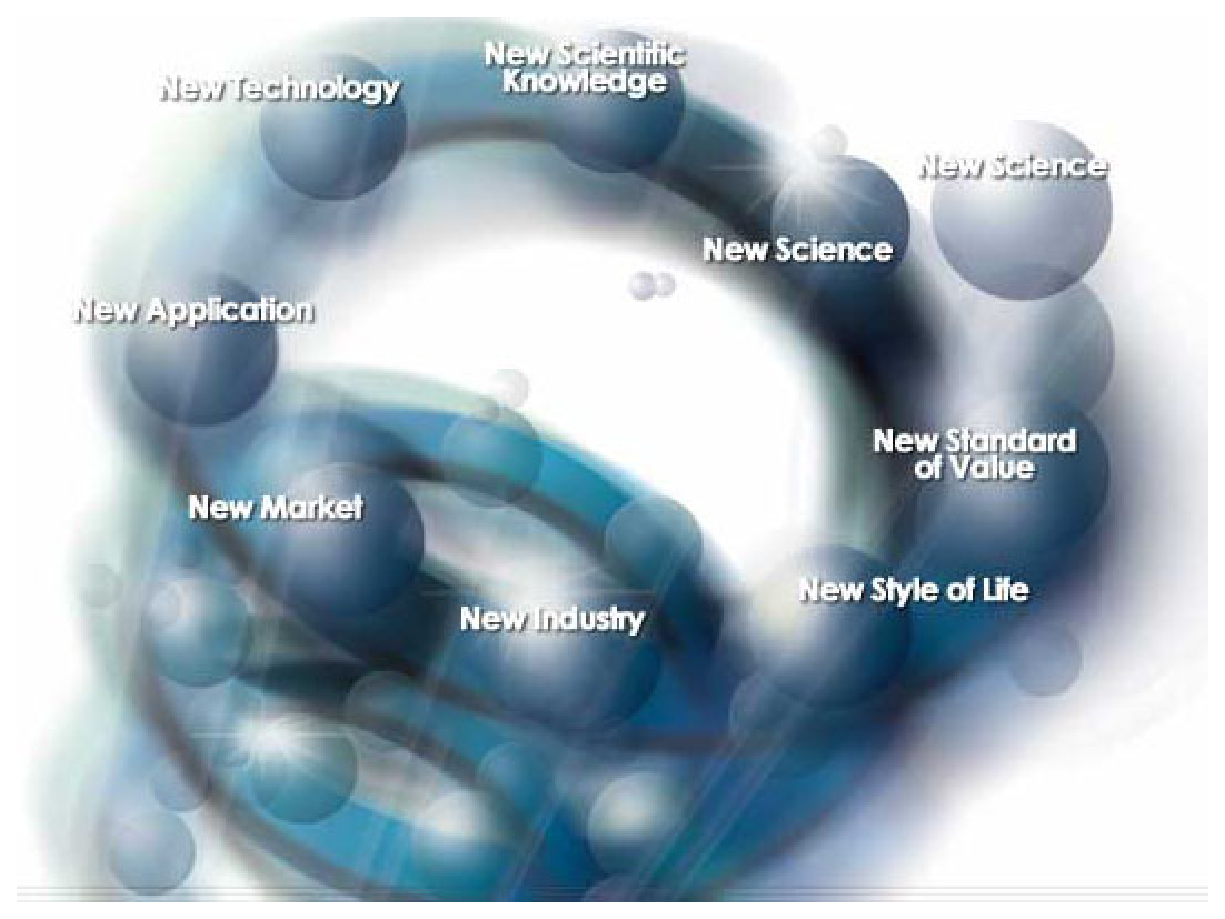
\includegraphics[clip,width=\textwidth]{Foreword/science-vision.ps}
\end{figure}
\end{center}

\begin{quote}
``人类之所以不断的扩展知识和见解,是基于想追究《真理是什么》的结果。
思维和艺术,宗教的不同之处在于是不是用他人都知道的手段去追究真理。
另外,在对真理的追究这一点上,日本语里《科学》的意思和本来的《思维》的意思也有不一样的地方。

新思维生成了新科学[把手段体系化的学问],这种新科学培育了技术和应用,打造了新产业。

新产业生成了人类的新的生活方式,产生了新的价值观,进而生成了新思维。'' 

\qquad 昼马辉夫

\end{quote}




%\input{Foreword/about_author}

%\newpage

%\input{Foreword/foreword2}

%\newpage

\chapter*{写在前面的话}

\qquad ``量子力学''已经诞生近百年,量子力学的应用范围也早已超越了``原子物理''
、``核物理''以及``粒子物理''的范畴,在``凝聚态物理''、``生物物理''、
``电子学''等广泛领域都有重要的应用,可以说``量子力学''已成为科学家的通用语言,
其重要性不言而喻。

量子力学是以原子物理的研究发展而来的,所以导论性量子力学课程与原子物理的关联很密切。
大多数情形下我们是通过对原子物理的学习来引入量子力学中的关键概念,量子力学理论框架建立后,
往往我们也是针对原子物理中的问题来应用量子力学。
原则上我们可将导论性的量子力学和原子物理看作一个整体来讲授和学习。

在本课程的前半部分主要讨论概念,并建立量子力学的基本理论,理解和思辩的成分较多,
类似于普通物理的学习。后半部分主要讨论量子力学的应用和近似方法,会涉及较多数学,
推导较多,概念相对较少,即便有也是基于数学基础上的概念,
学习的过程属于典型的理论物理课程。

不要期望一个学期就可掌握量子力学,对物理专业的学生来说量子力学是个反复学习的过程。
一般而言可分为四个阶段:(1)导论性的量子力学;
(2)高等量子力学,重视量子力学的形式体系,但一般不包括相对论性量子力学;
(3)量子场论,包括相对论性量子力学;(4)更高级的或更专门的量子场论。

本讲义适用于物理学专业或应用物理学专业的导论性量子力学,
对量子力学感兴趣的非物理专业学生也可参考。


关于``量子力学''国内外已有相当多的经典著作,但随着科学技术的不断进步,
特别是随着``量子力学''本身不断发展并应用到不同物理系统中,
我们的教材/讲义必须能反映这种最新进展。在内容的组织上,本讲义以``量子力学''为主线,
并在概念的引入,计算方法的应用中贯穿``原子物理''的知识,
并同时介绍``量子力学''的最新进展及其应用。

常用参考书:

\begin{enumerate}

\item{周世勋:《量子力学教程》,高等教育出版社;内容精练。}

\item{David J.Griffiths, \textbf{Introduction to Quantum Mechanics}, 机械工业出版社(2006).
美国本科生用标准教材,中英文版国内均有售。}

\item{J. J. Sakurai, \textbf{Modern Quantum Mechanics}, Revised Edition,
世界图书出版公司(2006). 美国研究生用标准教材,英文版国内有售。}
\end{enumerate}


更多参考书:


\begin{enumerate}


\item{曾谨言:《量子力学》卷I,科学出版社;内容深入浅出,讲解详细。}

\item{曾谨言:《量子力学导论》,北京大学出版社;适合本科生初学使用。}

\item{苏汝铿:《量子力学》,高等教育出版社;内容丰富,包括不少量子力学的新进展。}

\item{顾莱纳:《量子力学导论》,北京大学出版社;讲解详细,
是作者理论物理系列教材中的一本。}

\item{David Bohm, {\bf Quantum Theory}, Dover Publications (1989).
美国研究生用标准教材,有中译本。}

\item{Ramamurti Shankar, {\bf Principles of Quantum Mechanics}, Plenum Press, (1994).}

\item{P. A. M. Dirac, {\bf The Principles of Quantum Mechanics},
Clarendon Press, (1958). 量子力学经典著作,有中译本。}

\item{钱伯初、曾谨言:《量子力学习题精选与剖析(上)》,
科学出版社。}

\item{张宏宝:《量子力学教程学习辅导书》, 高等教育出版社。与周世勋书配合使用。}

\item{扬福家:《原子物理学》,高等教育出版社;有关于量子力学发展的大量背景资料和对相关物理概念的讨论,适合阅读。}

\item{杨桂林 等:《近代物理》,科学出版社(2004)}

\item{一本数学手册。}

\item{量子力学的最新进展与应用:
\\科学杂志新闻(Science News),
\url{http://news.sciencemag.org/}
\\自然杂志新闻(Nature News),
\url{http://www.nature.com/news/index.html}
\\科学的美国人(Scientific American Magazine),
\url{http://www.sciam.com/} 有中文版。
\\今日物理(Physics Today),
\url{http://www.physicstoday.org/}
\\物理世界(Physics World),
\url{http://physicsworld.com}

%\\物理评论聚焦(Physical Review Focus),
%\url{http://focus.aps.org/} 

}

\item{更专门的物理论文网站:
\\美国物理学会(APS)期刊的焦点论文,
\url{http://physics.aps.org/}
\\开放获取的物理论文网站(arXiv),
\url{http://cn.arxiv.org/} 
\\New Journal of Physics,
\url{http://iopscience.iop.org/1367-2630}

}

\end{enumerate}


\bigskip\medskip

\noindent
@季燕江\\

Email: jyj@sas.ustb.edu.cn\\
Git: \url{https://github.com/jiyanjiang/QMUSTB}\\
豆瓣: \url{http://site.douban.com/223228/}\\

20010年6月

\tableofcontents 
\setcounter{tocdepth}{2}


\newpage

\chapter{原子的观念}

\section{原子假说}

\begin{quotation}
“一尺之棰,日取其半,万世不竭。” \qquad 《庄子·杂篇·天下第三十三》
\end{quotation}


“原子”(atom)是物理学中的核心概念,费曼(R. P. Feynman,
1918-1988)甚至称其为物理学中最重要的概念\footnote{参考:
《费曼物理学讲义》卷I, 开篇; "If, in some cataclysm, all of scientific knowledge were to be
destroyed, and only one sentence passed on to the next generation of
creatures, what statement would contain the most information in the
fewest words? I believe it is the atomic  hypothesis that all things
are made of atoms-\emph{little particles that move around in
perpetual motion, attracting each other when they are a little
distance apart, but repelling upon being squeezed into one another}.
In that one sentence, you will see, there is an enormous amount of
information about the world, if just a little imagination and
thinking are applied.
"}。

\index{atom: 原子}

费曼假设因为某种灾难, 人类所有的知识都被毁灭了,
假如我们有机会告诉未来的文明一句话, 用最少的词汇传达最多的信息,
费曼的选择是“原子假说”(Atomic Hypothesis).
费曼以此来强调原子概念在物理学中的重要地位,
但我们知道原子假说早在2000多年前的古希腊就被当时的哲学家们提出了,
实际上原子是一个很古老的概念, 也不仅仅出现在古希腊哲学中,
如在印度哲学中有“极微说”。

\subsection{古希腊原子论}

古希腊原子论包含两个要点,首先存在原子,绝对的坚实和不可入,对应“有”,
并且存在不可分割的最小单元,原子一词在古希腊语中就是不可分割(indivisible)的意思。
其次存在虚空,虚空与原子相对,但它不可理解为“无”,而应理解为绝对的可入,绝对的可以容纳,
虚空使原子相互分离,
并提供了原子运动的舞台。原子和虚空是非常重要的概念,
它们不仅仅导向关于物性的科学, 如化学, 原子物理等; 还导向运动学,
“原子在虚空中的运动”在笛卡尔之后将被进一步理解为“质点在笛卡尔坐标系中的运动”。

原子论被后人认为是古希腊自然哲学的巅峰\footnote{关于古希腊的自然哲学与原子论,
可参考:海森堡(W. Heisenberg), 《物理学与哲学》, 第四章, 第25页;},
所谓自然哲学就是由自然出发, 用语言和逻辑去解释万事万物,
而不是通过神灵鬼怪的方式。泰勒斯(Thales,
生活于585BC)是这个传统的开始, 他一般也被认为是古希腊的第一位哲学家.
泰勒斯认为万物都可归为水。 恩培多克勒(Empedocles,
492BC-432BC)提出了水、火、土、气“四元素说”\footnote{与之类似佛教的物质论,
有所谓四大种“坚湿暖动”. 四元素和四大种很类似,
甚至我们可以直接建立: “坚即土, 湿即水, 暖即火, 动即气”这样的联系.
},后来又补充了以太, 作为构成天体和精神的第五元素。
为了解释世界的复杂和多样性,阿那克萨哥拉(Anaxagoras,
生活于500BC-428BC)提出了种子说,
即存在无数种元素,称之为种子,种子很小,小到感觉无法直接感觉到,只能通过理性把握。
面包里有肉的种子、血的种子和骨的种子,人吃了面包就能长身体,面包的种子就变成了人身体的结构。
种子说可看作是元素说的发展,只不过元素的种类变得无穷多了。

最早提出原子说的是留基伯(Leucippus,约 480 BC-约 420
BC),留基伯与阿那克萨哥拉同时代,原子说也可以看作是一种特殊的元素说,
只不过留基伯提出的元素是两种: 原子和虚空。 他认为:
“事物数目无限,它们总是相互转化。当原子坠入虚空并彼此交织时,世界就形成了。”
德谟克利特(Democritus,约 460 BC - 约 370
BC)是留基伯的学生,他认为原子可按照形状、大小进行分类,
而形状一词在古希腊语中与柏拉图的理念(idea)相同,
其实柏拉图的理念就是形状,但它强调那是理性而非感官能够把握的形,
用今天的话说就是“数学-几何学”。
柏拉图认为德谟克利特的原子说是他理念说的危险对手,
他甚至想带着自己的门徒去烧德谟克利特的著作。

这段今天读来会觉得很八卦, 其实回到2000多年前, 这是相当真实的.
首先在当时技术条件下, 著作全靠手抄, 拷贝数是有限的,
烧书是有可能彻底完成的. 其次, 古代哲学家及其门徒是政治性的团体,
他们聚集在一起是有共同政治目的的, 各门派的哲学都是综合性的.
系统化的古希腊哲学大致可分三部分,
最基础的是逻辑和方法(柏拉图是辩证法,亚里士多德是形而上学),
在此之上是自然哲学(相当于今天的科学),
而最上面的是伦理学(和政治学). 一个成功的哲学体系由逻辑和方法出发,
能够解释各种自然现象, 最后还要应用和落实在伦理学上。
柏拉图对德谟克利特原子论的反对,
不仅仅是因为他提出了一种竞争性的自然哲学,
更是因为这种自然哲学导向了一种柏拉图反对的伦理学和政治学.
这是和今天的科学完全不同的, 今天的研究是分科的,
每个学科都有自己独立的原理和问题,
我们今天不可能因为某种政治的理由去反对某个具体科学理论.


留基伯和德谟克利特的著作在今天还是失传了,
我们只能通过其他人的转述了解他们的思想,
比如亚里士多德在《物理学》中介绍并反驳了原子论的主张,
他论证了“不可能有任何连续事物是由不可分的事物合成的,
例如线不能由点合成, 线是连续的而点是不可分的.”\footnote{亚里士多德《物理学》第6卷
($231a21-231b20$);} 亚里士多德还论证了“对不可再分的物体而言,运动是不可能的”\footnote{亚里士多德《物理学》, 第6卷
($240b20-241a15$);}。

\index{Epicurus, 341 BC - 270 BC: 伊壁鸠鲁}

伊壁鸠鲁(Epicurus,341 BC - 270
BC)继承并进一步发展了原子假说,并在此基础上推出了“快乐主义”的伦理学,
伊壁鸠鲁学派是古希腊晚期重要的哲学流派之一,伊壁鸠鲁主义一度在希腊和罗马非常流行。
罗马诗人卢克莱修(Lucretius,约99BC-约55BC)是伊壁鸠鲁主义的信徒,
他流传的唯一著作《物性论》详细介绍了伊壁鸠鲁的自然哲学,
其中相当多的篇幅叙述了伊壁鸠鲁的原子思想。
到公元三世纪,罗马帝国时代的希腊作家第欧根尼·拉尔修编撰了关于古希腊各哲学流派哲学家的传记作品《名哲言行录》,
其中第十卷是关于伊壁鸠鲁的,第欧根尼·拉尔修在其中抄录了三封伊壁鸠鲁致友人的信,
其中致希罗多德书信(Letter to Herodotus\footnote{请阅读:
《自然与快乐:伊壁鸠鲁的哲学》 })是关于原子论的。


伊壁鸠鲁对德谟克利特原子假说的主要改进是(1)提出了“原子的偏转”(swerve),
即认为原子在运动过程中的任何一点都可能发生微小的偏转,
原子的运动不再是决定性的了,
伊壁鸠鲁认为这样就避免了德谟克利特的宿命论,
为“自由意志”保留了可能\footnote{“自由意志”在基督教神学中是很重要的概念,
因为如果人的行为完全是由原子的机械运动所决定(或完全由上帝的事先安排所决定),
那么个人就无需为自己的罪恶负责了。}。
也经常有人会把德谟克利特的原子论比作牛顿和拉普拉斯的机械力学,
而把伊壁鸠鲁引入“偏转”概念的原子论比作量子力学(“偏转”对应“量子跃迁”,量子力学中的跃迁也不是决定性的,而是几率性的)。
(2)伊壁鸠鲁认为原子不可能取所有的大小, 其大小是有上限的,
因为从来没有人见过原子, 另外原子的大小也是有下限的,
即不可能是任意小的.
伊壁鸠鲁强调“除形状、大小、重量和其他必然与形状联系在一起的性质外,
不应当认为原子还具有其他属性。”这里,
原子具有形状是原子论解释物性的基础,有形状就意味着有部分,
即在想象意义或数学意义下是可分的,那么在想象意义下原子是否无限可分呢?
伊壁鸠鲁仍然主张不能无限可分,因此有想象中的极小,没有形状,但却有体积,
并可用来度量体积。如果把亚里士多德和伊壁鸠鲁的观点做个比较的话,亚里士多德反对原子,
主张在自然和数学意义下都“无限可分”,而伊壁鸠鲁则正好相反,在自然和数学意义下都主张原子论。


在整个漫长的中世纪,原子论被欧洲人遗忘,哲学与诗歌和戏剧一起被作为异教的焚烧。
柏拉图的《蒂迈欧篇》是唯一流传的自然哲学著作,十字军东征后,亚里士多德的著作开始流传,
这为原子论的复兴奠定了基础。文艺复兴时期的1417年,意大利学者布拉乔利尼(Poggio
Bracciolini)在一个修道院里重新发现了卢克莱修的《物性论》并流传给当时的知识界。
随后,蒙田(Montaigne,1533-1592)、伽森狄
(Gassendi,1592-1655)等复活了伊壁鸠鲁的原子论思想,并通过玻意尔(Boyle,1627
-
1691)、道尔顿(Dalton,1766-1844)等实验物理学家的工作逐渐发展出了关于原子的近代理论。

\subsection{近代原子论}

\subsubsection{富兰克林油膜实验}

原子是超越经验的概念, 我们无法用感官直接感觉到原子的存在,
但有了原子的概念可以帮助我们融贯地理解很多日常观察到的现象。温伯格(Steven
Weinberg, 1933-)在《亚原子粒子的发现》中举例说:
“取一些盐溶解于一碗水里, 用原子论就很容易解释这一现象:
组成盐的原子分散到水原子之间的虚空中去了 ... 再例如,
一滴油滴在水面上, 它将扩散到一定的面积后才终止扩散,
用原子论很容易解释这种现象:
薄薄的油膜一直扩散到只有几个原子的厚度的时候, 才终止扩散。”
温伯格举的两个例子都是我们的日常经验,
这些现象即便在古代都应是人们熟悉的。第一个例子是古代原子论者经常举的例子,
第二个例子就是富兰克林油膜实验。

\index{Franklin's Oil-Drop Experiment: 富兰克林油膜实验}

富兰克林(Franklin)在1773年发现当把少量橄榄油放到水面上,
油膜最大只能覆盖有限的水面。假设橄榄油是由不可再分的体积有限的“原子”组成的,
我们就能由此估算原子的尺寸。富兰克林把一勺油,大约$5 cm^3$倒入池塘,
发现大约$2000 m^2$的水面被油膜覆盖了, 由此我们可估算出油膜的厚度,
大约是$2.5 nm$, 这可算是对原子尺寸的第一次定量估计了。

\begin{equation}
 d = \frac{V}{S} = \frac{{5 \times \left( {10^{ - 2} m} \right)^3
}}{{2 \times 10^3 m^2 }} = 2.5 \times 10^{ - 9} m
\end{equation}

$2.5 \times 10^{-9} m$即2.5纳米,这和细胞膜的厚度7-8纳米在同一数量级,考虑到细胞膜是两层油膜(脂双分子层)构成的,单层就是大约3.5纳米,富兰克林的估算在定量的意义下都已经很“准确”了。

结论:油这种物质存在基本单元(即存在“油的原子”),其大小是大约2.5纳米。

\subsubsection{道尔顿的原子假说}

随着工业化和近代化学的建立,原子学说获得了本质的进展。
1803年,英国科学家道尔顿(John Dalton, 1766 -
1844)提出了近代意义上的原子论:

\index{John Dalton, 1766 - 1844: 道尔顿}

\begin{enumerate}

\item{ 原子是组成化学元素的、非常微小的、不可再分割的物质微粒。
在化学反应中原子保持其本来的性质。}

\item{ 同一种元素的所有原子的质量以及其他性质完全相同。不同元素
的原子具有不同的质量以及其他性质。原子的质量是每一种元素的原子
的最根本特征。}

\item{ 有简单数值比的元素的原子结合时,原子之间就发生化学反应
而生成化合物。化合物的原子称为复杂原子。}

\item{ 一种元素的原子与另一种元素的原子化合时,他们之间存在
简单的数值比。}

\end{enumerate}

{\bf 例1:} $2H{}_2 + O_2
\mathbin{\lower.3ex\hbox{$\buildrel\textstyle\rightarrow\over
{\smash{\leftarrow}\vphantom{_{\vbox to.5ex{\vss}}}}$}} 2H_2 O$,
两倍体积的氢气与一倍体积的氧气恰好完全反应,生成水;或:
1克氢气与8克氧气完全反应生成9克水。由此可猜想:水分子由两个氢原子,
一个氧原子构成。


\subsubsection{法拉第电解定律}


人类很早就知道了电现象, 丝绸摩擦玻璃棒带正电, 毛皮摩擦橡胶棒带负电,
这是关于静电的研究. 金属可以导电, 并导致相应物理效应,
这是所谓动电的研究. 电学的研究在19世纪达到了很高的成就,
并与更古老的学问——磁学——联系了起来,
电磁学的最后完成很大程度上可归功于法拉第和麦克斯韦两位英国科学家,
法拉第是实验物理学家,而麦克斯韦则是位理论物理学家,类似于第谷和开普勒的关系。

1833年,法拉第(Michael Faraday, 1791 -
1867)发现电解定律:电解时,在电极上析出或溶解掉的
物质的重量,与通过电极的电量成正比;如通过的电量相同,
则析出或溶解掉的不同物质的摩尔数\footnote{1摩尔(mol)
物质包含阿佛加德罗常数$N_A$个粒子。}相同。


\begin{figure}[h]
\begin{center}
  % Requires \usepackage{graphicx}
  \includegraphics[width=6cm]{AtomIdea/faradaylaw.ps}\\
  \caption{法拉第电解水实验}
\end{center}
\end{figure}


\index{Faraday's  laws of electrolysis: 法拉第电解定律}

{\bf 例2:}电解水实验,$H_2 O \rightarrow 2H^ +   + O^{2 - } $,
法拉第发现每电离出1克氢气(或8克氧气),需要96485库仑电量( 定义:$1F
= 9.6485 \times 10^4
C$)。由此我们可以猜想:1)原子中可能有“标准”带电粒子——“电子”
存在,电荷是“量子化”的;
2)电磁相互作用是原子组成分子及物质聚集(气、液、固三态)的物理原因。
如果我们知道电子的电荷,就可以计算出阿佛加德罗常数:$N_A  = F/e$。

法拉第工作的意义是把化学与物理学联系起来,成为统一的科学。


\subsection*{阅读材料}

\begin{itemize}
  \item 张竹明 译, 亚里士多德《物理学》
  
  \item 王玮玮
等译,《自然与快乐: 伊壁鸠鲁的哲学》

\end{itemize}


\section{电子的发现}

19世纪末期, 关于真空管的实验很流行.
科学家们发现在真空管内加上电极和电压, 随着电压的增大,
会发生真空放电现象, 在真空管的阴极会发出阴极射线(cathode rays).
阴极射线是什么, 具体说是一种粒子,
还是一种波动(电磁波)就成了19世纪末期科学家们争论的一个热门问题。

\subsection{汤姆逊实验}

\begin{figure}[h]
\begin{center}
  % Requires \usepackage{graphicx}
  \includegraphics[width=5cm]{AtomIdea/perrin.ps}\\
  \caption{佩林实验}\label{Perrin experiment}
\end{center}
\end{figure}



1895 佩林通过用量电器(electrometer)收集阴极射线表明这种射线带负电,
实验如图(\ref{Perrin experiment}). 英国科学家们认为阴极射线是粒子,
而德国科学家们则倾向于波. 为了验证自己的想法, 1897
年英国科学家汤姆逊(Thomson)进行了实验.
汤姆逊认为阴极射线就是带电粒子流, 质量为$m$, 电荷为$e$,
通过测量阴极射线在外加电场(或磁场)真空管内的偏转,
汤姆逊测量了带电粒子的荷质比(specific charge),
这种粒子正是我们现在所说的“电子”(electron)。

\begin{figure}[h]
\begin{center}
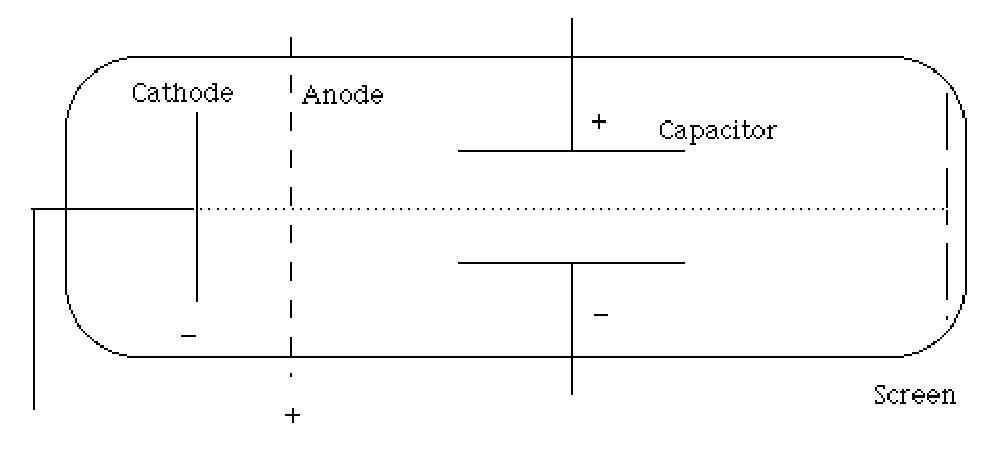
\includegraphics[clip,width=8cm]{AtomIdea/1-1.eps}
\caption{汤姆逊实验示意图}
\end{center}
\end{figure}

\begin{enumerate}
\item{首先,用阴极射线照射电量计,发现电量计逐渐积累了负电荷;(说明粒子流带负电)}

\item{在阴极射线管内加强磁场,发现阴极射线会弯曲;(带电粒子在磁场内可作圆周运动)}

\item{在电容器(capacitor)上加电压$V$,发现阴极射线会向上弯曲;}

\item{在垂直方向加合适的磁场B,可以使阴极射线重新回到原点,抵消因为加电场所引起的弯曲;}

\end{enumerate}

实验的第4个步骤说明运动粒子在磁场内所受洛仑兹力与库仑力正好抵消:$|ev
\times B| = |eE|$,可计算出粒子运动速度: $v =
E/B$。我们可以测量电场为零情况下,粒子运动半径r,$m\frac{{v^2 }}{r}
= evB$,可计算出电子的荷质比为:$e/m = \frac{E}{{rB^2 }}$。$E$, $B$,
$r$都是实验可测量的,这样我们可求出粒子(电子)的荷质比。

\index{Specific charge: 荷质比}

电子荷质比的现代数据:$e/m_e  = 1.7588 \times 10^{11} C/kg$

与质子的“荷质比”比较: $e/m_p  = 1F/1g = 9.6485 \times 10^7 C/kg$

可见:$m_p /m_e  = 1822$, 说明电子比氢原子(质子)轻将近2000倍。
后来汤姆逊还使用同样的方法测量了光电效应中光电子的荷质比,
发现与阴极射线中电子的荷质比相同,实际上它们是同一种粒子——电子。

\subsection{密立根油滴实验}

\begin{figure}[htbp]
\begin{center}
\includegraphics[width=10cm]{AtomIdea/millikan.ps}
\includegraphics[width=10cm]{AtomIdea/millikan1.ps}
\caption{密立根油滴实验}
%\label{default}
\end{center}
\end{figure}

\index{Millikan's oil drop experiment: 密立根油滴实验}

1911年,密立根(Millikan)油滴实验直接地证明了电荷是量子化的,最小
单元电量(对应电子电量)是:$e = 1.602 \times 10^{ - 19} C$。据说为了获得稳定的高电压,密立根在做实验的时候自己制造了约1000个铅电池。


这样根据荷质比数值,可以计算出电子质量为:$m_e  = 9.109 \times 10^{
- 31} kg$

同样我们也可计算出阿佛加德罗常数的数值:

\begin{equation}
N_A  = F/e = 6.02 \times 10^{23} 
\end{equation}

\index{Avogadro's constant: 阿佛加德罗常数}

{\bf 例3 由阿佛加德罗常数,估算原子的尺度:}\\
设mole质量为$A$,mole体积$V$,密度:$\rho  = A/V$, 原子半径为: $r$;
原子的数密度为:$\frac{1}{{\left( {{\textstyle{4 \over 3}}\pi r^3 }
\right)}} = \frac{{N_A }}{V} = \frac{{N_A }}{{\left(
{{\raise0.5ex\hbox{$\scriptstyle A$} \kern-0.1em/\kern-0.15em
\lower0.25ex\hbox{$\scriptstyle \rho $}}} \right)}}$,
由此可得到原子半径公式:

\begin{equation}
r = \left( {\frac{{3A}}{{4\pi N_A \rho }}} \right)^{1/3}
\end{equation}

根据固体的质量密度$\rho $数据,我们可估计出不同原子的半径:

\begin{table}[h]
\begin{center}
\caption{不同原子的半径}
\begin{tabular}{|c|c|c|c|}

\hline  元素&   质量数$A$&    质量密度$\rho$($g / cm^3$)&
原子半径($nm$)\\
\hline $Li$&  7&  0.7&   0.16\\
\hline $Al$& 27& 2.7& 0.16\\
\hline $S$&  32& 2.07&    0.18\\
\hline $Cu$&  63& 8.9&    0.14\\
\hline $Pb$&  207& 11.34&    0.19\\
\hline
\end{tabular}
\end{center}
\end{table}

计算发现,不同原子的半径都是埃的数量级($10^{ - 10} m$ ).


\subsection{电子经典半径}

根据爱因斯坦质能关系和电磁场能量密度关系,
我们还可以估算出电子的尺度, 称之为电子的经典半径(electron classical
radius)。

\index{Electron classical radius: 电子的经典半径}

电子的总能量可分别用爱因斯坦质能关系和电磁场能量密度对全空间积分表示,
并且应当是相等的:

\begin{equation}
W = m_e c^2  = \int {\frac{{\varepsilon _0
}}{2}E^2 d\tau }
\end{equation}

假设电子是一个电荷均匀分布的球体,电子的半径为$r_e$,\\
当$r \ge r_e$,电场强度为:$E(r \ge r_e ) = \frac{1}{{4\pi
\varepsilon _0 }} \cdot \frac{e}{{r^2 }}$。\\
当$r < r_e$,电场强度为: $E(r < r_e ) = \frac{1}{{4\pi \varepsilon
_0 }} \cdot \left( {\frac{{r^3 }}{{r_e ^3 }}} \right) \cdot
\frac{e}{{r^2 }} = \frac{{er}}{{4\pi \varepsilon _0 r_e ^3 }}$。

对应能量为:

\begin{eqnarray*}
W(r < r_e ) &=& \int_{0}^{r_e} \frac{\varepsilon _0 }{2} | E(r< r_e)|^2 4\pi r^2 dr = \frac{e^2 }{40 \pi \varepsilon _0 r_e } \\
W(r \ge r_e ) &=& \int_{r_e}^{\infty} \frac{\varepsilon _0 }{2} | E(r \ge r_e)|^2 4\pi r^2 dr = \frac{e^2 }{8\pi \varepsilon _0 r_e }
\end{eqnarray*}

加起来就是:

\begin{equation}
W = \frac{3 }{5} \frac{e^2}{ 4\pi \varepsilon _0 r_e} 
\end{equation}

能量积分与电荷分布细节有关,假设电荷均匀分布在半径$r_e$的球面上的话,$E(r< r_e) = 0$,计算出电子的能量为:

\begin{equation}
W = \frac{1}{2} \frac{e^2}{ 4\pi \varepsilon _0 r_e} 
\end{equation}

忽略掉在$\frac{e^2}{ 4\pi \varepsilon _0 r_e}$前方的因子$3/5$或$1/2$,电子的能量是:

\begin{equation}
\frac{e^2}{ 4\pi \varepsilon _0 r_e} 
\end{equation}

根据狭义相对论,电子的能量还是“质量倍的光速平方”($m_e c^2 $),由:

\begin{equation}
m_e c^2  = \frac{e^2}{ 4\pi \varepsilon _0 r_e} 
\end{equation}

我们定义电子的经典半径(Electron classical radius, $r_e$)为:

\begin{equation}
r_e  = \frac{{e^2 }}{{4\pi \varepsilon _0 m_e c^2 }} \approx 2.818 \times 10^{-15} m
\end{equation}

$10^{-15}m$也叫1飞米(femtometer,$fm$)。可见电子尺度远小于原子尺度,至少小5个数量级,相对原子的大小而言,
我们可以把电子当作“点”处理。电子经典半径不能反映电子的实际线度,
它仅是电子半径上限的一个估算。现代物理学研究表明,
电子半径小于$10^{-18}m$, 但不知道下限是多少。


\subsection{原子的汤姆逊模型}


我们现在知道原子整体是电中性的, 其中包含带负电的电子, 电子质量很小,
尺寸也很小, 原子中也必然包括正电部分, 其质量很大,
但正电部分在整个原子中的分布是未知的, 可能是集中地分布的,
也可能是均匀地分布于整个原子内等等。

\index{Thompson model: 汤姆逊模型}

现在就需要我们构造出一个关于原子的模型,
成功的原子模型至少应能解释一些物理现象,
比如当时已被大家熟知的元素周期律、光谱现象等; 另一方面, 很重要的,
这个原子模型应当是稳定的, 因为我们的世界是稳定存在的,
不可能设想组成我们世界的原子是不稳定的, 或只能存在于须臾之间.

我们可以假设原子中的正电部分象电子一样也是集中分布的,
比如某种正电子, 为了简化考虑, 我们假设所有电荷都是不动的,
这时就是一个静电学问题. 对一个由正、负点电荷组成的静电体系,
我们可以设法构造出受力平衡, 但我们发现这种平衡是不稳定的,
总存在某种形式的微小扰动能够破坏受力平衡,
即这种正电荷集中分布的静电体系是不稳定的.

剩下的选择自然是假设正电不是集中分布的,
比如正电部分均匀地分布在整个原子,
而电子对称地镶嵌在正电背景中(比如可以考虑氢原子),
可以证明这样做可以达到受力平衡, 并且是稳定平衡.
汤姆逊就是基于以上考虑提出了这样一个怪怪的原子模型,
即认为原子中的正电荷均匀分布在整个原子中,而电子则镶嵌在其中。
为了保证系统的稳定性,电子只能镶嵌在特定的位置上,如一个电子,必须
位于原子的中心,两个电子,则必须对称地分布在中心的两侧,三个或
更多个电子则必须是环状分布的,这似乎可以解释元素的周期性.
形象地说这就是个西瓜模型, 西瓜子是电子, 而西瓜瓤是正电部分。

\index{Planetary model: 行星模型}

今天看来, 汤姆逊模型确实有点怪, 但它却是一个“稳定”的模型,
相反原子的行星模型(planetary model)是一种更直观的模型,
但根据经典电动力学却是一种“不稳定”的模型. 更加美妙的是,
根据汤姆逊模型, 竟然能解释氢原子光谱莱曼系的第一支.
因此在卢瑟福散射实验之前,
原子的汤姆逊模型是科学家们最看好的一个原子模型.

\begin{figure}[h]
\begin{center}
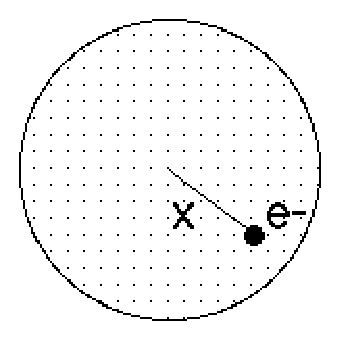
\includegraphics[clip,width=4cm]{AtomIdea/1-2.eps}
\caption{氢原子的汤姆逊模型}
\end{center}
\end{figure}

{\bf 例4 氢原子的汤姆逊模型}

考虑系统的稳定性,假设电子偏离平衡位置(球心)$x$,氢原子半径$a$,根据高斯定理,仅半径$x$球体内正电荷会与电子发生吸引。

\begin{equation}
F = m\ddot x =  - \left( {\frac{1}{{4\pi \varepsilon _0 x^2 }}}
\right)\left( {\frac{{x^3 }}{{a^3 }}} \right)e^2  =  - \left(
{\frac{1}{{4\pi \varepsilon _0 }}} \right)\left( {\frac{{e^2
}}{{a^3 }}} \right)x
\end{equation}

微分方程:$\ddot x + \omega ^2 x = 0$,频率为:$\omega  = \sqrt
{\frac{{e^2 }}{{4\pi \varepsilon _0 a^3 m}}} $,计算可得:$\nu =
\frac{\omega }{{2\pi }} = 2.5 \times 10^{15} Hz,\lambda  =
1200\mathop A\limits^o $
与氢原子光谱赖曼系第一支(Lyman-$\alpha$)吻合,但该模型无法解释氢原子其他的谱线。

\begin{figure}[h]
\begin{center}
  % Requires \usepackage{graphicx}
  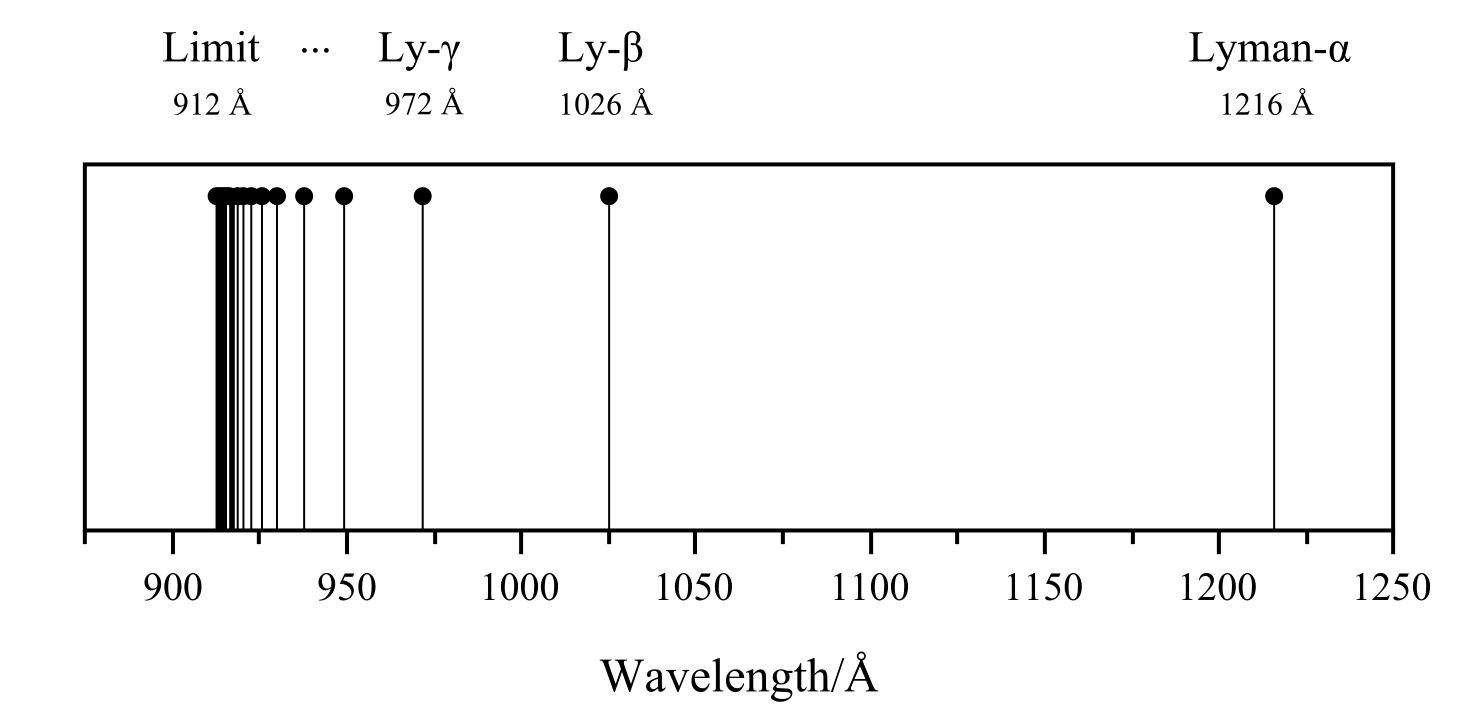
\includegraphics[width=10cm]{AtomIdea/LymanSeries.png}\\
  \caption{氢原子光谱赖曼系}\label{Lyman Series for Hydrogen atom}
\end{center}
\end{figure}



\subsection*{物理常数}

\begin{itemize}
  \item 阿佛加德罗常数: $N_A= 6.022 \times 10^{23} mole^{-1}$
  \item 法拉第常数: $F=9.648 \times 10^4 C \cdot mole^{-1}$
  \item 电子电量: $e = 1.602 \times 10^{-19} C$
  \item 电子质量: $m_e =9.109 \times 10^{-31}kg$
  \item 质子质量: $m_p = 1.673 \times 10^{27} kg$
  \item 光速:$c = 2.998 \times 10^8 m \cdot s^{-1}$
\end{itemize}

\subsection*{单位换算}

在粒子物理中, 我们通常用兆电子伏($MeV = 10^6 eV $)来表示粒子的质量.
请将电子质量($m_e$), 质子质量($m_p$)换算为$MeV$.

解: 根据相对论质能关系: $E=m_0 c^2$, 这里$m_0$是静止质量.
对电子而言,

\begin{equation*}
E = 9.109 \times 10^{-31} (3.0 \times 10^8)^2 = 8.2 \times 10^{-14}
J
\end{equation*}

相当于:

\begin{equation*}
\frac{8.2 \times 10^{-14}}{1.602 \times 10^{-19}} = 5.1 \times 10^5
eV = 0.51 \text{MeV}
\end{equation*}

假设质子“静能量”为$x$MeV,

\begin{equation*}
\frac{m_e c^2}{M_p c^2}=\frac{0.51}{x}
\end{equation*}

解出:

\begin{equation*}
x = 0.51 \cdot \frac{M_p}{m_e} =0.51 \times 1822 = 932
\end{equation*}

即质子“静能量”为932MeV, 或约1GeV.

\subsection*{阅读材料}


\begin{itemize}

  \item 原子的核心含义是“不可再分”,或按亚里士多德的“修正”,是某个层次(或技术条件)下的“不可再分”。我们有电的原子——电子,光的原子——光子,物质的原子——往往是分子(保持物质化学性质的最小单位)……

回到原子的本意——“不可再分”,原子在今天科学知识下的对应应是基本粒子(Elementary Particles),电子和光子都是基本的(不可再分的),原子核不是,它可以分为质子和中子,统称为重子(Baryons),重子也不是基本的,它由夸克组成,而夸克是基本的。

相关知识,请进一步阅读维基百科:Elementary particle

\url{http://en.wikipedia.org/wiki/Elementary_particle}

\item 原子物理标准的英文教材: B H Brandsden and C. J. Joachain, Physics of atoms and
  molecules. 
  
\item 阅读新科学家(New Scientist)文章: ``Roundest objects in the world
created'' \url{http://sinaurl.cn/7xVw3}

阿佛加德罗计划:如何通过完美的硅晶球精确定义千克(kg,国际单位制中的质量单位)。

\url{http://www.acpo.csiro.au/avogadro.htm}

\item 斯蒂芬·温伯格,《亚原子粒子的发现》
  
\item M Veltman, 《神奇的粒子世界》
  
\end{itemize}


\section{卢瑟福模型}

\begin{quotation}
“这是我一生中碰到的最不可思议的事情。就好像你用一颗15英寸大炮去轰击一张纸而你竟被反弹回的炮弹击中一样。” \qquad 卢瑟福
\end{quotation}

\subsection{卢瑟福散射}

卢瑟福(Rutherford, 1871-1937)是汤姆逊的学生,
为了验证汤姆逊的原子模型,1906-1913
年间\footnote{第一次世界大战发生于1914年-1918年,
如果没有卢瑟福的工作,
人类关于原子物理和原子核物理的研究就会大大推迟, John Schiffer
推测核武器的出现将推迟到第三次世界大战,
这将给人类带来极大的灾难。\url{http://physicsworld.com/cws/article/multimedia/2011/sep/01/rutherfords-big-discovery-100-years-later}}他使用高能(MeV量级)$\alpha$粒子轰击金属薄膜(foil).
由于入射粒子能量很高,
卢瑟福预期所有入射粒子应几乎不受影响地穿过金属薄膜,
但实验结果却表明有约1/8000的入射粒子被散射回来了, 即散射角大于90度.
对此,卢瑟福有非常形象的描述\footnote{"It was quite the most incredible event that ever happened to me in
my life. It was almost as incredible as if you fired a 15-inch shell
at a piece of tissue paper and it came back and hit you.
"}:

\index{Rutherford scattering: 卢瑟福散射}

\begin{quote}

这是我一生中碰到的最不可思议的事情.
就好像你用一颗15英寸大炮去轰击一张纸而你竟被反弹回的炮弹击中一样.

\end{quote}

15英寸大炮是当时大英帝国海军口径最大的火炮,
卢瑟福用这种形象的语言告诉我们,
原子的正电部分不可能均匀地分布在整个原子中, 即汤姆逊模型是错的.


\begin{figure}[h]
\begin{center}
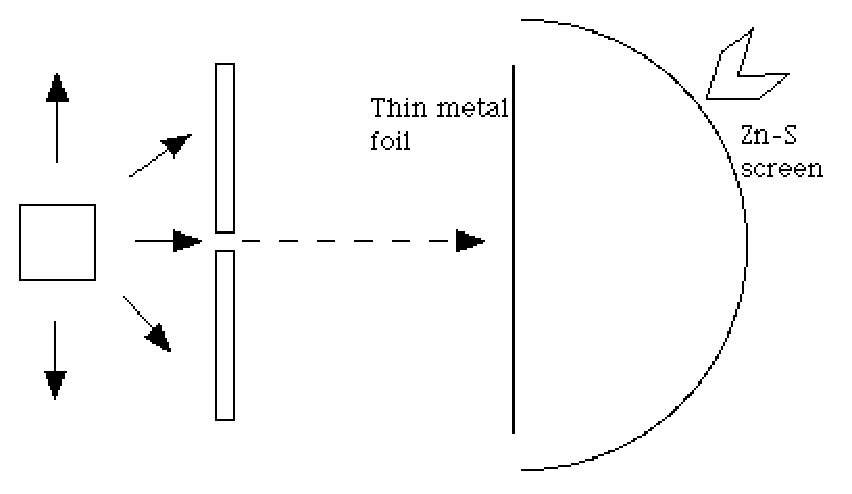
\includegraphics[clip,width=8cm]{AtomIdea/1-3.eps}
\caption{卢瑟福散射示意图}
\end{center}
\end{figure}


\begin{enumerate}
\item{按汤姆逊模型, $\alpha
$粒子在原子半径处受力最大,其上限为:$F = \frac{{2e(Ze)}}{{4\pi
\varepsilon _0 R^2 }}$, $\alpha $粒子飞越原子时间约为:$\Delta t =
2R/v$; 这样$\alpha $粒子在碰撞过程中最大动量改变为:$\Delta p =
F\Delta t = \left( {\frac{{e^2 }}{{4\pi \varepsilon _0 }}}
\right)\left( {\frac{{4Z}}{{Rv}}} \right)$, 其中:$\frac{{e^2
}}{{4\pi \varepsilon _0 }} = 1.44(fm \cdot Mev)$, $1fm = 1 \times
10^{ - 15} m$, 经常在计算中用到;可以计算出
粒子在汤姆逊模型下最大可能偏转角为:$\theta  = \frac{{\Delta p}}{p}
= 3 \times 10^{ - 5} \frac{Z}{{E_\alpha }}rad$, ($1 rad = 180^o/ \pi
\simeq 57.3^o$)。}

\item{估计$\alpha $粒子与电子的碰撞导致的最大偏转:$m_\alpha  /m_e
= 7300$,电子质量在碰撞过程中几乎可以忽略,最大可能偏转为:$\theta
= \frac{{2m_e }}{{m_\alpha  }} \approx 10^{ - 4} rad $ .}

\item{多次碰撞效应,由于金属膜很薄, 每次偏转的角度都是随机的,所以即便考虑多次碰撞, 最终发生大角度
偏转也是不可能的。取膜厚$1\mu m = 10^{-6}m$, 相当于有$10^4$层原子,
被散射$10^4$次后出射, 取最大可能偏转角度为$10^{-4}rad$,
即便每次都是最大角度散射, 每次都向一个方向偏转,
最大散射角也仅为$1rad$, 考虑到每次偏转方向都是随机的,
更合理的估计是$\sqrt N \theta = \sqrt{10^4} \cdot 10^{-4} rad  =
10^{-2} rad$, 这显然无法解释大于$90^o$的散射。}

\end{enumerate}


\subsection{卢瑟福模型}

\begin{figure}[h]
\begin{center}
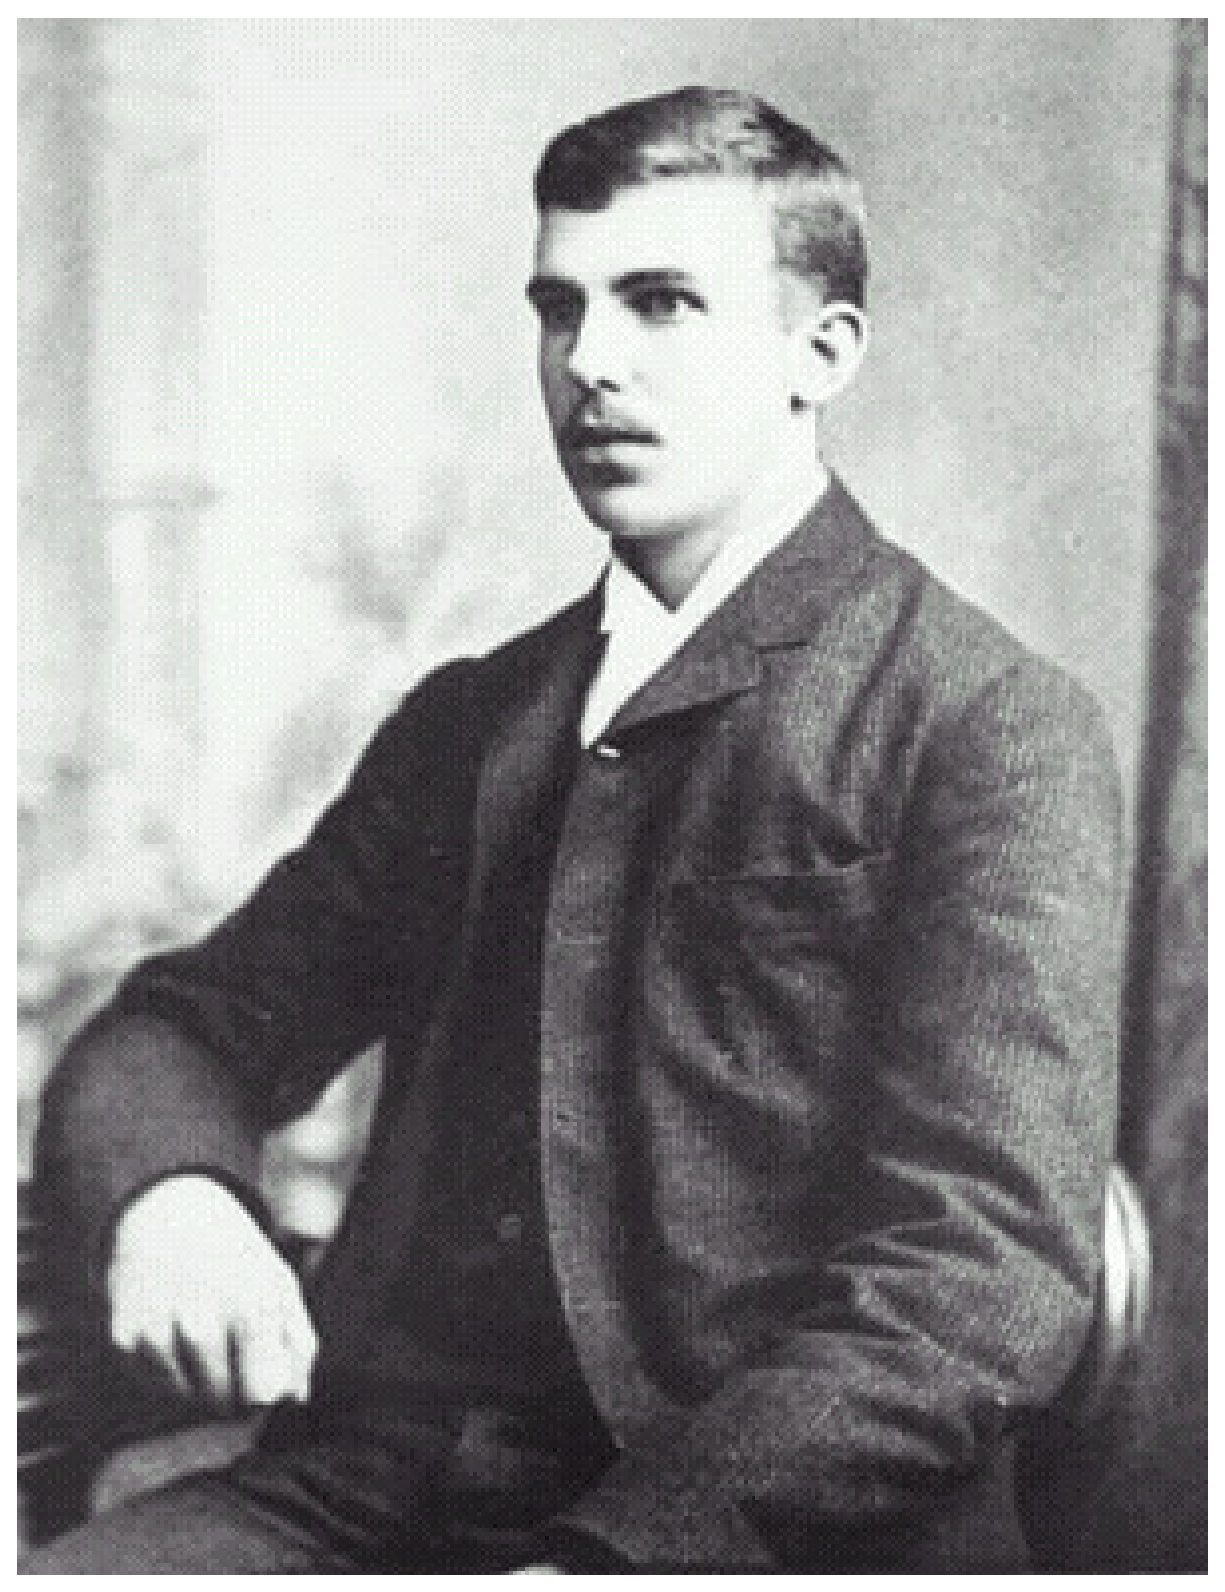
\includegraphics[clip,width=4cm]{AtomIdea/rutherford.ps}
\caption{卢瑟福}
\end{center}
\end{figure}

为解释卢瑟福散射, 卢瑟福提出原子内的正电荷集中分布在原子中心极
小区域内,即原子是由原子核和核外电子组成, 并推导出了卢瑟福散射公式,
成功地解释了卢瑟福散射的实验曲线。

\index{Rutherford model: 卢瑟福模型}

由于入射粒子质量远小于靶材料原子核质量,假设靶原子核静止,问题
简化为标准的中心力场问题。(由理论力学知识:粒子在中心力场中运动,
粒子轨迹为圆锥曲线,在散射问题中,粒子由无穷远入射,所以其轨迹
是双曲线的一支,核在双曲线的焦点上。)


\begin{figure}[h]
\begin{center}
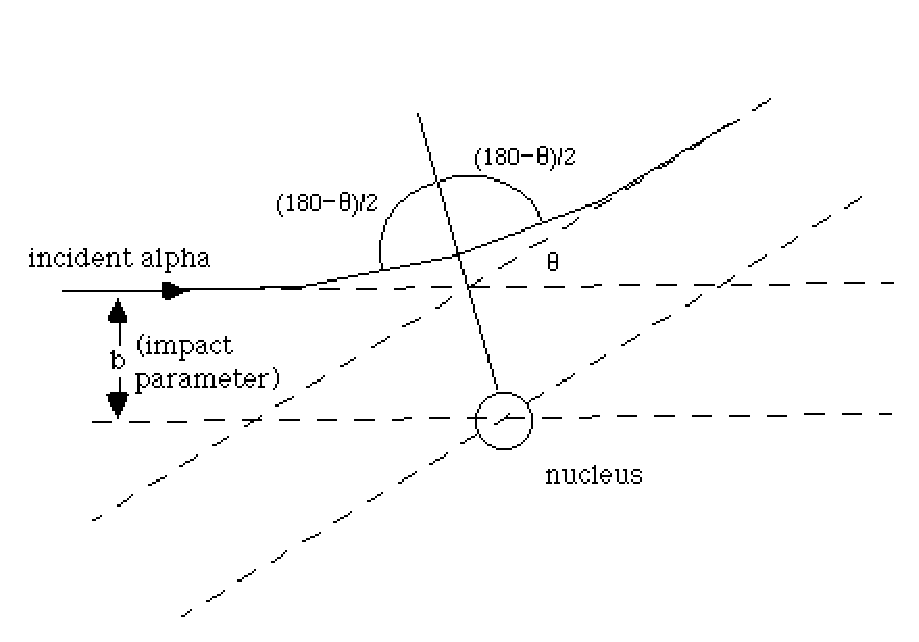
\includegraphics[clip,width=8cm]{AtomIdea/1-4.eps}
\caption{库仑散射}
\end{center}
\end{figure}

碰撞为弹性碰撞,$\alpha $
粒子出射动量与入射动量大小不改变,只改变方向,设方向改变
$\theta$;

\begin{figure}[h]
\begin{center}
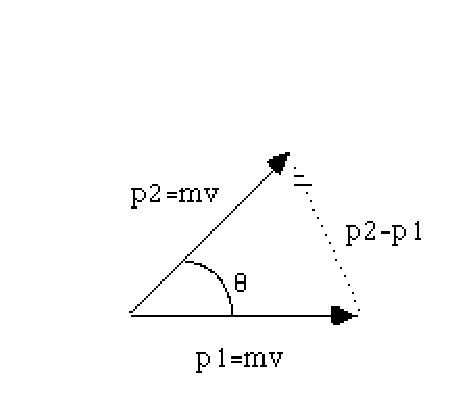
\includegraphics[clip,width=6cm]{AtomIdea/1-5.eps}
\caption{散射引起的动量变化}
\end{center}
\end{figure}

散射引起的动量变化:$\Delta p = p_2  - p_1  = 2mv\sin \left(
{\theta /2} \right)$

根据牛顿定律:

\begin{equation}
\Delta p = \int_{t_1 }^{t_2 } {Fdt}  = \int
{F\frac{{dt}}{{d\varphi }}d\varphi }  = \int {\frac{{Fd\varphi
}}{{\dot \varphi }}} 
\end{equation}

这里:$F = \frac{{Z_1 Z_2 e^2 }}{{4\pi \varepsilon _0 r^2 }}\hat
r$

所以:$\Delta p = \int {\left( {\frac{{Z_1 Z_2 e^2 }}{{4\pi
\varepsilon _0 }}} \right)\frac{{\hat rd\varphi }}{{r^2 \dot
\varphi }}}  = \int {\left( {\frac{{Z_1 Z_2 e^2 }}{{4\pi
\varepsilon _0 }}} \right)} \frac{m}{{mr^2 \dot \varphi }}\hat
rd\varphi $

中心力场中,角动量守恒:$mr^2 \dot \varphi  = L = mvb$

所以\footnote{这个积分的计算可参考:
杨福家《原子物理学》第三版,pp16。}:

\begin{equation}
\Delta p = \left( {\frac{{Z_1
Z_2 e^2 }}{{4\pi \varepsilon _0 }}} \right)  \frac{1}{{vb}}\int
{\hat rd\varphi } 
\end{equation}

即:

\begin{equation}
2mv\sin ({\raise0.5ex\hbox{$\scriptstyle \theta $}
\kern-0.1em/\kern-0.15em \lower0.25ex\hbox{$\scriptstyle 2$}}) =
\left( {\frac{{Z_1 Z_2 e^2 }}{{4\pi \varepsilon _0 }}} \right)
 \frac{1}{{vb}} 2\cos ({\raise0.5ex\hbox{$\scriptstyle
\theta $} \kern-0.1em/\kern-0.15em \lower0.25ex\hbox{$\scriptstyle
2$}})
\end{equation}

瞄准距离(碰撞参数):

\begin{equation}
b = \left( {\frac{{Z_1 Z_2 e^2 }}{{4\pi
\varepsilon _0 }}} \right)  \frac{1}{{mv^2 }} 
\frac{{\cos ({\textstyle{\theta  \over 2}})}}{{\sin
({\textstyle{\theta  \over 2}})}} = \frac{1}{2}\left( {\frac{{Z_1
Z_2 e^2 }}{{4\pi \varepsilon _0 }}} \right) \frac{1}{{E_k }}
 \cot ({\textstyle{\theta  \over 2}})
\end{equation}


定义:$a = \frac{{Z_1 Z_2 e^2 }}{{4\pi \varepsilon _0 E_k }}$, 这里:
$E_k  = \frac{{mv^2 }}{2}$, 就得到库仑散射公式:


\begin{equation}
b = \frac{a}{2} \cot \left( {\frac{\theta }{2}} \right)
\label{column}
\end{equation}


{\bf 例5 角度大于$\theta $的库仑散射}

由于我们无法在实验室中测量瞄准距离$b$,应当设法在公式
(\ref{column}) 中设法消去参数$b$; 假设靶上仅一个原子.

\begin{figure}[h]
\begin{center}
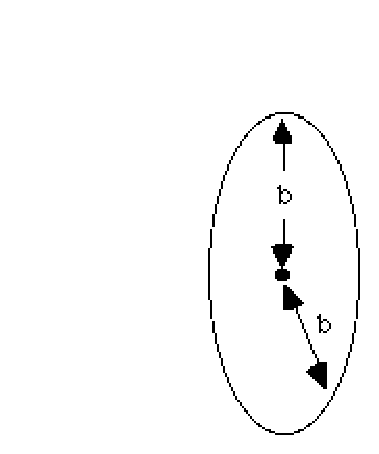
\includegraphics[clip,width=5cm]{AtomIdea/1-6.eps}
\caption{瞄准距离$b$}
\end{center}
\end{figure}

\index{Coulomb Scattering: 库仑散射}

由库仑散射公式,入射到瞄准距离$b$内的$\alpha
$粒子对应的散射角大于$\theta $(库仑相互作用更强)。
所以散射角度大于$\theta $的散射几率为:$P( \ge \theta ) =
\frac{{\pi b^2 }}{A}$, 其中$A$为金属箔(靶)的面积。

考虑实际的金属箔,面积:$A$,厚度:$t$,密度:$\rho $
;假设金属箔很薄,使金属箔内各原子之间不互相遮挡,则金属箔内有$nAt
$个独立的``散射核'',只要入射$\alpha$粒子落在$nAt
$个``散射核''附近的$\pi b^2$内,
对应的就是散射角大于$\theta$的散射事件。

这里 $n$是``散射核数密度'':$n = \frac{{N_A }}{V} = \frac{{\rho N_A
}}{M}$,$M$是mole质量;所以对实际金属箔,散射角大于$\theta
$的散射几率为:$P( \ge \theta ) = nAt \cdot \frac{{\pi b^2 }}{A} =
\pi b^2 t \cdot \left( {\frac{{\rho N_A }}{M}} \right)$, 即:


\begin{equation}
\label{theta}
P( \ge \theta ) = \frac{{\pi t\rho N_A }}{M}\left(
{\frac{1}{2} \cdot \frac{{Z_1 Z_2 e^2 }}{{4\pi \varepsilon _0 E_k
}}} \right)^2 \left( {\cot {\raise0.5ex\hbox{$\scriptstyle \theta
$} \kern-0.1em/\kern-0.15em \lower0.25ex\hbox{$\scriptstyle 2$}}}
\right)^2
\end{equation}

现在公式(\ref{theta})中各项,都是实验中可以测量的了。


{\bf 讨论:}当$\theta  = 0$ 附近,即小角散射,$P( \ge 0) \to \infty
$, 这显然是不合理的,这是因为小角散射对应大的碰撞参数$b$,
原子之间互不遮挡这个前提条件就不成立了。
此时,核外电子对入射电子的作用就必须考虑了。
在碰撞参数达到原子大小时,整个原子呈电中性,库仑散射根本不会发生。
因此,对小角散射,不考虑核外电子屏蔽效应的卢瑟福散射公式是不正确的。

\subsection{卢瑟福散射公式}

由公式$P( \ge \theta ) = nt\pi b^2  = nt\pi \left( {{\textstyle{a
\over 2}}\cot ({\raise0.5ex\hbox{$\scriptstyle \theta $}
\kern-0.1em/\kern-0.15em \lower0.25ex\hbox{$\scriptstyle 2$}})}
\right)^2 $ , 求落在立体角$d\Omega  = 2\pi \sin \theta d\theta $
内的几率:

\begin{equation}
\frac{{dP}}{{d\Omega }} = \frac{1}{{2\pi \sin \theta }} \cdot
\frac{{dP}}{{d\theta }} = \frac{1}{{2\pi \sin \theta }} \cdot
\left( {\frac{{a^2 nt\pi }}{4}} \right)\frac{d}{{d\theta }}(\cot
{\textstyle{\theta  \over 2}})^2 
\end{equation}

利用微分关系:$\frac{d}{{d\theta }}\left( {\cot {\textstyle{\theta
\over 2}}} \right)^2  =  - \frac{{\cos {\textstyle{\theta  \over
2}}}}{{(\sin {\textstyle{\theta  \over 2}})^3 }}$


所以:$\frac{{dP}}{{d\Omega }} =  - \left( {\frac{{nta^2 }}{{16}}}
\right) \cdot \frac{1}{{(\sin {\textstyle{\theta  \over 2}})^4
}}$,负号表示$\theta $越大,散射到大于$\theta $的几率越小。
只考虑大小的话:$dP(\theta ) = \frac{{a^2 d\Omega }}{{16\left( {\sin
{\textstyle{\theta  \over 2}}} \right)^4 }}nt$


如有$N$个入射粒子,则散射到$d \Omega $方向上的粒子为:$dN(\theta ) =
ntN\left( {\frac{a}{4}} \right)^2  \cdot \frac{{d\Omega }}{{(\sin
{\textstyle{\theta  \over 2}})^4 }}$. 定义微分截面(Differential
cross section):

\index{Differential cross section: 微分截面}

\begin{equation}\label{differential cross section formula}
\sigma _c (\theta ) = \frac{{dN(\theta )}}{{Nntd\Omega }} =
\frac{{dP(\theta )}}{{ntd\Omega }} = \frac{{d\sigma (\theta
)}}{{d\Omega }} = \left( {\frac{a}{4}} \right)^2  \cdot
\frac{1}{{(\sin {\textstyle{\theta  \over 2}})^4 }},
\end{equation}

即卢瑟福公式\footnote{严格说, 这个公式差个``负号''。}.
考虑公式(\ref{differential cross section formula})中第二个``等号'',
$\sigma_c(\theta) = \frac{dP(\theta)}{nt d \Omega}$, 我们可得到:

\begin{equation}
    \frac{dP(\theta)}{d \Omega}
    = nAt \cdot \frac{\sigma_c (\theta)}{A}
\end{equation}

上式可与$P(\ge \theta) = nAt \cdot \frac{\pi b^2}{A}$比较。我们发现:
$\frac{dP(\theta)}{d \Omega}$中的$\sigma_c (\theta)$的地位和$P(\ge
\theta)$中的$\pi b^2$相同。由此我们可以得到$\sigma_c(\theta)$,
即微分散射截面的物理意义,


\begin{quote}
入射粒子被散射到$\theta $ 方向单位立体角内每个原子的有效散射截面,
具有面积的量纲。
\end{quote}

\begin{figure}[h]
\begin{center}
  % Requires \usepackage{graphicx}
  \includegraphics[width=5cm]{AtomIdea/cross_section.ps}\\
  \caption{散射截面}
\end{center}
\end{figure}



现在考虑公式(\ref{differential cross section
formula})中第三个``等号'', $d P(\theta)$
正比于每个散射中心附近的截面积(cross section) $d \sigma$,
对应的散射立体角为 $d \Omega = 2 \pi \sin \theta d \theta$,
容易计算出,

\begin{equation}
\frac{d \sigma (\theta)}{d \Omega} = \frac{b}{\sin \theta} \cdot
\frac{db}{d \theta} = (\frac{a}{4})^2 \cdot \frac{1}{(\sin
\frac{\theta}{2})^4} .
\end{equation}

\subsection{卢瑟福模型的困难}

\begin{figure}[h]
\begin{center}
  % Requires \usepackage{graphicx}
  \includegraphics[width=4cm]{AtomIdea/spiral.ps}\\
  %\caption{}\label{}
\end{center}
\end{figure}


卢瑟福模型可以解释卢瑟福散射的实验数据,但它无法解释原子的稳定性,和原子光谱的经验公式\footnote{1885年,瑞士中学教师巴尔末(Balmer)发现了关于氢原子光谱的经验公式:\\
波数:$\tilde \nu  = \frac{1}{\lambda } = \frac{4}{B}\left(
{\frac{1}{{2^2 }} - \frac{1}{{n^2 }}} \right),n =
3,4,5...$,B=364.56nm。这个公式被称为:巴尔末公式,它所描述的一组谱线被称为巴尔末系。}。
作为练习, 我们可以计算最简单的原子——氢原子——的寿命,
假设氢原子中唯一的电子围绕原子核(即质子)作匀速圆周运动,
电子的圆周运动可分解为垂直方向上两个电偶极子的迭加,
根据电偶极辐射功率公式我们可以估算多久电子的能量会耗尽而落到原子核上.
估算表明, 卢瑟福原子是非常不稳定的, 很短时间(大约$10^{-10}
s$)后电子就会落到原子核上,从而导致原子的崩溃。


\subsubsection*{练习:估算卢瑟福氢原子寿命}

根据经典电动力学\footnote{郭硕鸿, 《电动力学》, 第二版, pp226,
习题11},带电粒子$e$作半径为$a$的非相对论性圆周运动,
回旋频率为$\omega$, 远处的辐射能流密度为:

\begin{equation*}
\vec S=\frac{\mu_0 \omega^4 e^2 a^2}{32\pi^2 c R^2} (1+\cos^2
\theta) \vec e_R
\end{equation*}


估算卢瑟福氢原子的寿命. ($\epsilon_0 = 8.854 \times 10^{-12} F \cdot
m^{-1}, \mu_0 = 12.566 \times 10^{-7} H \cdot m^{-1}$)

\begin{quote}
    解:电子在半径为$a$正圆轨道上运动, 应满足:

\begin{equation*}
    m \frac{v^2}{a} = m \omega^2 a = \frac{1}{4 \pi \epsilon_0}
    \frac{e^2}{a^2}
\end{equation*}

解出动能$K$为:$\frac{mv^2}{2} = \frac{1}{8 \pi \epsilon_0}
\frac{e^2}{a}$, 总能量为:

\begin{equation*}
E = K + V = - \frac{1}{8 \pi \epsilon_0} \frac{e^2}{a}
\end{equation*}

两边求微分:

\begin{equation*}
d E = \frac{e^2}{8 \pi \epsilon_0 a^2} da
\end{equation*}


当$da$取负数, 即电子运动半径缩小时, $d E$ 也取负数,
系统能量是减少的, 这部分减少的能量将通过电磁辐射被辐射掉.
系统总的辐射功率$P$是辐射能流$\vec S$对面积圆的积分, $P = \oint \vec
S \cdot d \vec \sigma$, $d \sigma = 2 \pi R \sin \theta R d \theta =
2 \pi R^2 \sin \theta d \theta$, 因此\footnote{参考:林璇英, 张之翔,
《电动力学题解》, 科学出版社, 2002. pp362}:

\begin{equation*}
P = \int_0^{\pi} \frac{\mu_0 \omega^4 e^2 a^2}{32\pi^2 c R^2}
(1+\cos^2 \theta)2 \pi R^2 \sin \theta d \theta =
\frac{e^2a^2\omega^4}{6\pi \epsilon_0 c^3}
\end{equation*}

能量守恒: $dE = P dt  = \frac{e^2}{8 \pi \epsilon_0 a^2} da$,
轨道缩小的速率为:

\begin{equation*}
\frac{da}{dt} = \frac{8 \pi \epsilon_0 a^2}{e^2} \cdot
\frac{e^2a^2\omega^4}{6\pi \epsilon_0 c^3} = \frac{4 \omega^4 a^4
}{3 c^3}
\end{equation*}

上式是速度量纲的, 由$m \omega^2 a = \frac{1}{4 \pi \epsilon_0}
\frac{e^2}{a^2}$, 解出: $\omega^2 = \frac{e^2}{4 \pi \epsilon_0 m
a^3}$, 代入$\dot a$的表达式,

\begin{equation*}
\frac{da}{dt} = \frac{e^4}{12 \pi^2 \epsilon_0^2 m^2 a^2 c^3}
\end{equation*}

即:

\begin{equation*}
dt = \frac{12 \pi^2 \epsilon_0^2 m^2 c^3}{e^4} a^2 da
\end{equation*}

两边积分, $t$从$0 \to \tau$(原子寿命), $a$ 从$0 \to a_0$,

\begin{equation*}
\tau = \frac{12 \pi^2 \epsilon_0^2 m^2 c^3}{e^4} \cdot
\frac{a_0^3}{3} = \frac{4 \pi^2 \epsilon_0^2 m^2 c^3 a_0^3}{e^4}
\end{equation*}

\index{Electron classical radius: 电子的经典半径}

考虑到电子的经典半径:

\begin{equation*}
r_e = \frac{e^2}{4 \pi \epsilon_0 m_e c^2} = 2.818 \times 10^{-15} m
\end{equation*}

氢原子寿命$\tau$可重新表示为\footnote{此结果可与杨福家《原子物理学》第三版pp26中的估算进行比较;}:

\begin{equation*}
\tau = \frac{a_0^3}{4 c r_e^2}
\end{equation*}

取氢原子半径为$a_0 = 0.1 nm$, 得到$\tau \approx 1 \times 10^{-10}
s$, 更真实的估计是取$a_0 = 0.5 nm$, 此时$\tau \approx 1 \times
10^{-11} s$.

\end{quote}


\subsection{用几何关系推导库仑散射公式}

\begin{figure}[h]
\begin{center}
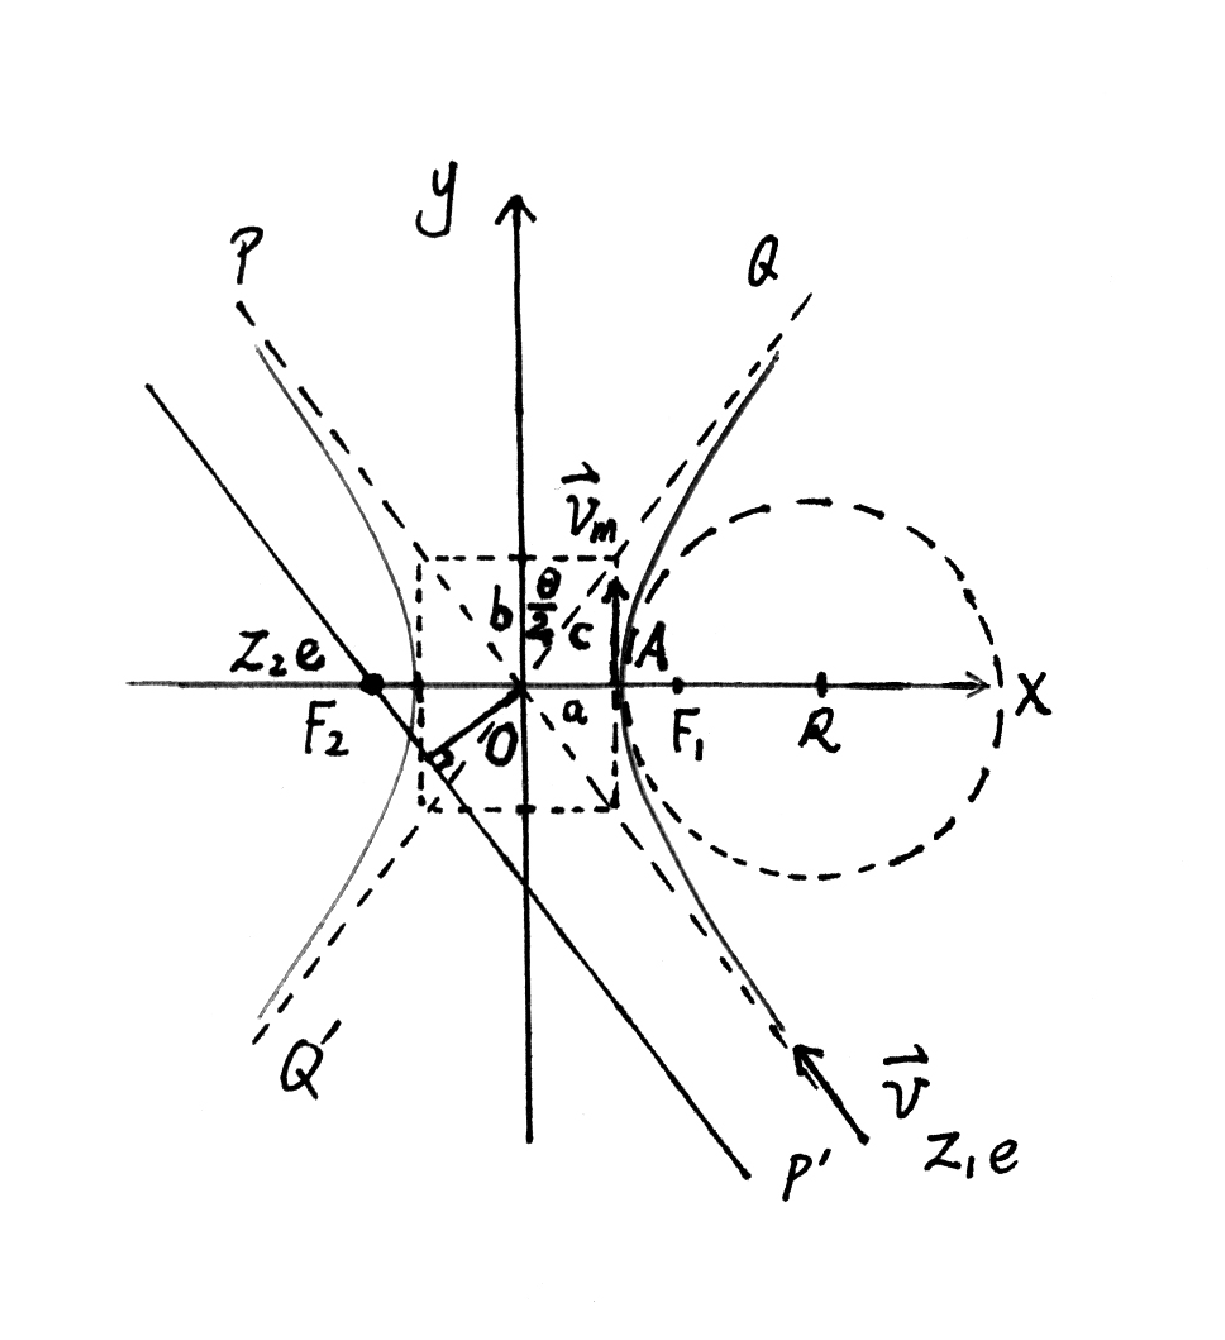
\includegraphics[clip,width=8cm]{AtomIdea/1-7.ps}
\caption{对卢瑟福散射而言, 入射粒子轨迹是双曲线的一支;}
\end{center}
\end{figure}


\index{Coulomb force: 库仑力}

根据经典力学,粒子受中心力场(库仑力、万有引力)散射,轨迹是圆锥曲线,对卢瑟福散射而言,
入射粒子轨迹是双曲线的一支,根据几何关系我们也可以得到库仑散射公式(公式\ref{column})。

假设入射粒子$Z_{1}e$以速度$\vec v$由无穷远入射, 其轨迹是双曲线
$\frac{{x^2 }}{{a^2 }} - \frac{{y^2 }}{{b^2 }} =
1$的右半支,靶原子核$Z_{2}e$位于左焦点$F_2$处。$\left| {OF_2 }
\right| = c$, 入射粒子距靶原子核最近距离为$r_m$,$r_m  = a + c$。

粒子出射方向与入射方向的夹角为$\theta $,则:

\begin{equation*}
\begin{array}{l}
b = a\cot {\textstyle{\theta  \over 2}}\\
c = a\csc {\textstyle{\theta  \over 2}}\\
\end{array}
\end{equation*}

瞄准距离为:$\tilde b = c\cos {\textstyle{\theta  \over 2}} = b$


\index{curvature: 曲率}

在入射粒子距靶原子核最近距离位置$\overrightarrow {OA}
$,曲率(curvature)为:

\begin{equation*}
k = \frac{1}{R} = \frac{{\left| {\dot x\ddot y - \ddot x\dot y}
\right|}}{{\left( {\dot x^2  + \dot y^2 } \right)^{3/2} }}
\end{equation*}


根据双曲线的参数方程(以$\Theta$为参数建立):

\begin{equation*}
\begin{array}{l}
 x = a\sec \Theta  \\
 y = b\tan \Theta  \\
\end{array}
\end{equation*}

$\overrightarrow {OA} $对应于$\Theta  = 0$,因此:

\begin{equation*}
\left\{ \begin{array}{l}
 \dot x = 0 \\
 \dot y = b \\
 \ddot x = a \\
 \ddot y = 0 \\
 \end{array} \right.
\end{equation*}

\index{radius of curvature: 曲率半径}


可求出最近位置$\overrightarrow {OA} $时曲率半径(radius of
curvature)为:

\begin{equation*}
R = \frac{1}{k} = \frac{{b^2 }}{a} = b\cot {\textstyle{\theta \over
2}},
\end{equation*}


入射粒子此时的运动方程为:$m\frac{{v_m^2 }}{R} = \frac{{Z_1 Z_2 e^2
}}{{4\pi \varepsilon _0 r_m^2 }}$。

因此:$R = mv_m^2 r_m^2 \left( {\frac{{Z_1 Z_2 e^2 }}{{4\pi \varepsilon _0 }}} \right)^{ - 1}  = b\cot {\textstyle{\theta  \over 2}}$

入射粒子在中心力场中运动,满足角动量守恒:$mvb = mv_m r_m $;

因此:$R = 2\frac{{mv^2 }}{2}b^{\not 2} \left( {\frac{{Z_1 Z_2 e^2 }}{{4\pi \varepsilon _0 }}} \right)^{ - 1}  = \not b\cot {\textstyle{\theta  \over 2}}$

即:$2E_k b\left( {\frac{{Z_1 Z_2 e^2 }}{{4\pi \varepsilon _0 }}} \right)^{ - 1}  = \cot {\textstyle{\theta  \over 2}}$

可得库仑散射公式:

\begin{equation*}
b = \frac{{Z_1 Z_2 e^2 }}{{4\pi \varepsilon _0 }}\frac{1}{{2E_k
}}\cot {\textstyle{\theta  \over 2}}
\end{equation*}

\subsection*{练习}

\begin{itemize}
\item{质量为$m_1$的入射粒子被质量为$m_2$($m_2 \le m_1$)}的静止靶核弹性散射,试证明:入射粒子在实验室坐标系中最大可能偏转角$\theta_L $由下式决定:$\sin \theta _L  = \frac{{m_2 }}{{m_1 }}$。

\item{(1)动能为5.00MeV的$\alpha$粒子被金核以$90^o$散射时,它的瞄准距离(碰撞参数)为多大?
(2)如果金箔厚$1.0\mu
m$,则入射$\alpha$粒子束以大于$90^o$散射(称为背散射, back
scattering)的粒子数是全部入射粒子的百分之几?}

\item{一束$\alpha$粒子垂直入射到一重金属箔上,试求$\alpha$粒子被金属箔散射后,散射角大于$60^o$的$\alpha$
粒子数与散射角大于$90^o$的$\alpha$粒子数之比。}

\item{4.5$MeV$的$\alpha$粒子与金($Au$)核对心碰撞时的最小距离($r_m$)是多少?}

\end{itemize}


\subsection*{阅读与思考}

\begin{itemize}

\item{卢瑟福散射提供了以散射为手段研究物质结构的方法,1967年,美国发射了一个月球探险飞船,上面搭载了一个$\alpha $源,利用$\alpha $粒子对月球表面的卢瑟福散射,分析了月球表面的成分,并把结果发回地球。
这一结果与1969年阿波罗飞船从月球取回样品所作分析结果基本符合,以此为标志,
卢瑟福散射成为材料分析的有力手段,按此原理制成的卢瑟福谱仪已成为标准的商品。

请阅读维基百科词条:Rutherford backscattering spectrometry. 
\url{http://en.wikipedia.org/wiki/Rutherford_backscattering_spectrometry}
}

\end{itemize}


\chapter{波粒二象性}

\section{黑体辐射}

\begin{quotation}
``......重要的是用一种尽可能保守的方式来进行工作,就是说,只有那些已被证明为绝对必要的变化才应该被引入到现存的理论中。''\qquad 普朗克
\end{quotation}

\subsection{预备知识}

\index{Thermal radiation: 热辐射}

热辐射是热量传递方式之一。物体之间的空间存在辐射场,
辐射场是各种频率的电磁波在空间的分布。
物体可通过发射、吸收电磁波的过程与其周围的辐射场交换能量。
辐射场可看作是光子气,即把辐射场看作是许多不同频率,
但全部以光速$c$运动彼此完全独立的光子体系 \footnote{参考:M. W.
泽门斯基, R. H. 迪特曼, {\bf 热学和热力学}, p511;}。
我们一般考虑处在热平衡状态下的物体与辐射场,它们有相同的温度$T$。

为定量描述辐射场,及辐射场与物体间的能量交换,引入:辐射场能量的分布函数:
$f(\nu ,\hat k,r,t)d\nu d\Omega$,

其中: $\hat k$
代表光子传播方向单位矢量,r是空间位置矢量,t是时间。如果辐射场是均匀的,则f与r无关,
如辐射场是恒定的,则f与t无关,如辐射场是各向同性的,则f与$\hat k$无关。

定义1:辐射场能量的谱密度$u(\nu )$:

\begin{equation*}
u(\nu ,r,t) = \int {f(\nu ,\hat k,r,t)d\Omega }  = \int_0^{2\pi }
{d\varphi \int_0^\pi  {d\theta \sin \theta f(\nu ,\theta ,\varphi
,r,t)} }
\end{equation*}

假设辐射场是各向同性的,则:

\begin{equation}
u(\nu ,r,t) = 4\pi f(\nu ,r,t)
\end{equation}

定义2:辐射通量谱密度$\Delta j(\nu )$:

\begin{eqnarray*}
\Delta j(\nu ,r,t) & =  & \int\limits_{2\pi } {cf(\nu ,\hat k,r,t)\hat k
\cdot \Delta S d\Omega }  \\
{} & = & \int_0^{2\pi } {d\varphi
\int_0^{{\raise0.5ex\hbox{$\scriptstyle \pi $}
\kern-0.1em/\kern-0.15em \lower0.25ex\hbox{$\scriptstyle 2$}}}
{d\theta \sin \theta \cos \theta  \cdot cf(\nu ,\theta ,\varphi
,r,t)} }
\end{eqnarray*}

假设辐射场是各向同性的,$\Delta S$是单位面元矢量,$\hat k \cdot
\Delta S = \cos \theta $,则:

\begin{equation}
\Delta j(\nu ,r,t) = \pi cf(\nu,r,t)\Delta S
\end{equation}

\begin{figure}[h]
\begin{center}
  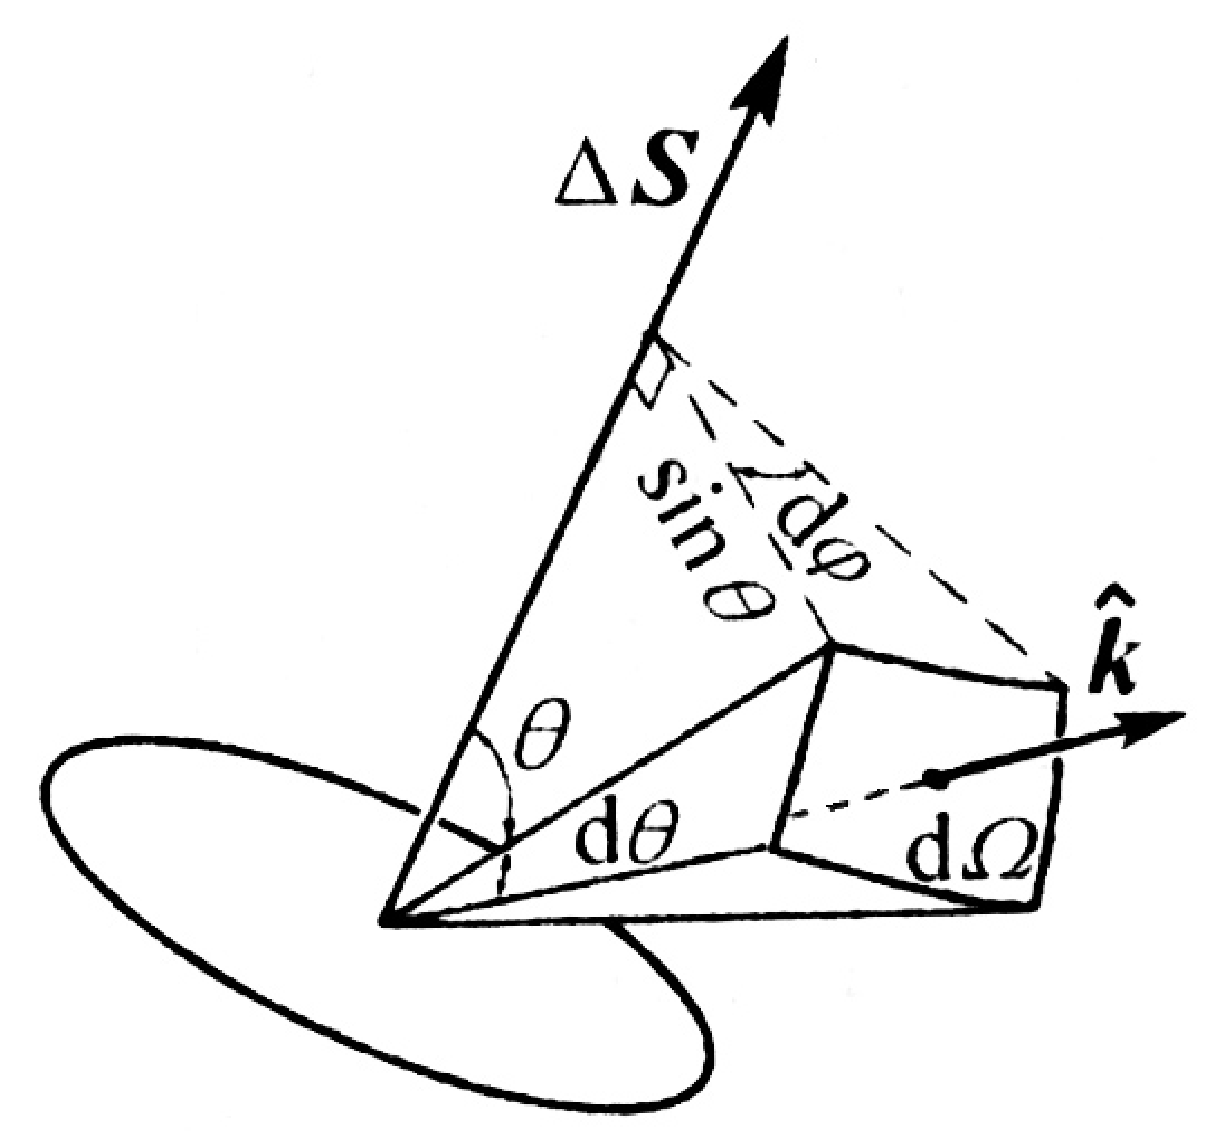
\includegraphics[width=5cm]{Duality/2-1.ps}\\
  \caption{球坐标表示立体角}\label{2-1}
\end{center}
\end{figure}

上式中的$c$是电磁辐射能流的速率(即光速),对立体角的积分限于面元$\Delta S$的一侧($2\pi$)。积分时取以面元法线$\Delta S$为极轴的球坐标系,用$\theta$、$\varphi$来表示传播方向$\hat k$。


定义如下辐射场与物体间交换能量的物理量:
\begin{enumerate}
    \item 辐射本领(物体表面单位面积发出的辐射通量)谱密度:$r(\nu ) = \frac{{dj(\nu )}}{{dS}}$
    \item 辐射照度(照射在物体表面单位面积上的辐射通量)谱密度:$e(\nu ) = \frac{{dj'(\nu )}}{{dS}} = \pi cf = \frac{c}{4}u(\nu )$
    \item 吸收本领:$\alpha (\nu ) = \frac{{dj''(\nu )}}{{dj'(\nu )}}$,即吸收的辐射通量密度与照射的辐射通量密度之比,显然此比值在0,1之间。
\end{enumerate}

\index{Kirchhoff's law: 基尔霍夫定律}

基尔霍夫热辐射定律(Kirchhoff's
law):在热平衡状态下的辐射场,应是均匀、恒定、各向同性的,其能谱密度$u_T
(\nu )$ 应仅与平衡时温度T,和$\nu $有关,即$u_T (\nu
)$是一个与物质无关的普适函数,称为:热辐射的标准能谱。

在平衡态下,任一表面积上发出的能量$r(\nu ,T)$与吸收的能量$\alpha (\nu )\frac{{dj'}}{{dS}} = \alpha (\nu )e(\nu ,T)$
相等。即:$r(\nu ,T) = \alpha (\nu )e(\nu ,T)$。

所以:

\begin{equation}
\frac{{r(\nu ,T)}}{{\alpha (\nu )}} = e(\nu ,T) = \frac{c}{4}u_T (\nu )
\end{equation}

即:辐射本领与吸收本领成正比,比值只与$\nu $和T有关。

\subsection{黑体辐射}

绝对黑体:物体的吸收本领$\alpha (\nu
,T)$与$\nu$和T无关,恒等于1,简称黑体。 即绝对黑体辐射本领:$r_b
(\nu ,T) = \frac{c}{4}u_T (\nu )$,
所以只要测量绝对黑体的辐射本领,即可获得热辐射的标准能谱。

\index{Black body: 黑体}

和质点一样,黑体是理想的物理模型,实际物质不可能是真正的黑体。我们一般用开有小孔,内壁粗糙的空腔来表示它。光射进小孔后,要经过内壁无穷次反射后,才有非常微弱的光从小孔重新射出,孔越小,从小孔处反射出的光越微弱,近似可看作光全部被吸收。用这种方法人们可以制备非常理想的黑体,并测量黑体辐射谱。

\begin{figure}[h]
\begin{center}
  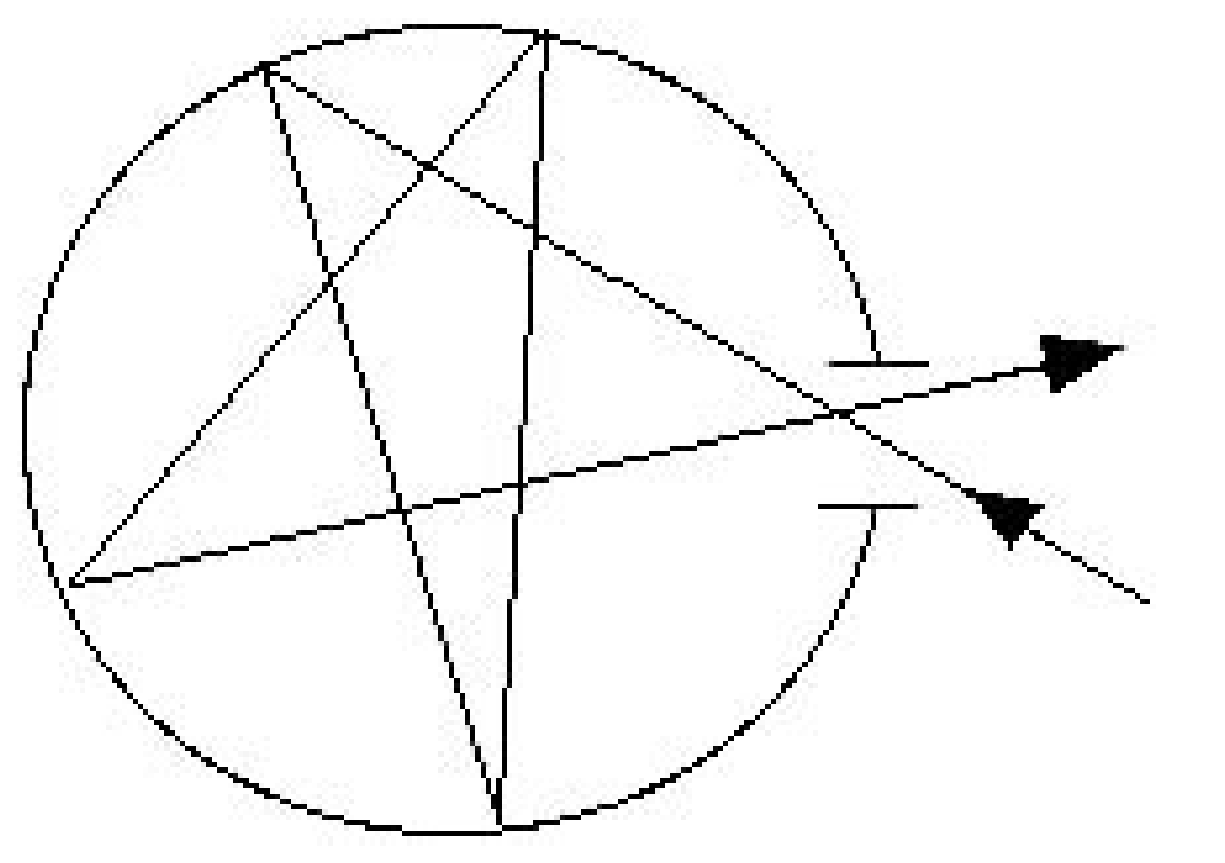
\includegraphics[width=5cm]{Duality/2-2.ps}\\
  \caption{绝对黑体的制备}\label{blackbody}
\end{center}
\end{figure}

需要注意的是,这里的黑体是小孔,而非空腔。这种黑体对我们来说并不陌生,典型的例子就是炼钢的高炉,或动画片《大闹天宫》中太上老君炼丹的炉子。对空腔(炼丹炉)加热,我们可测量由小孔(黑体)辐射出的不同温度下的热辐射曲线。

\begin{figure}[h]
\begin{center}
  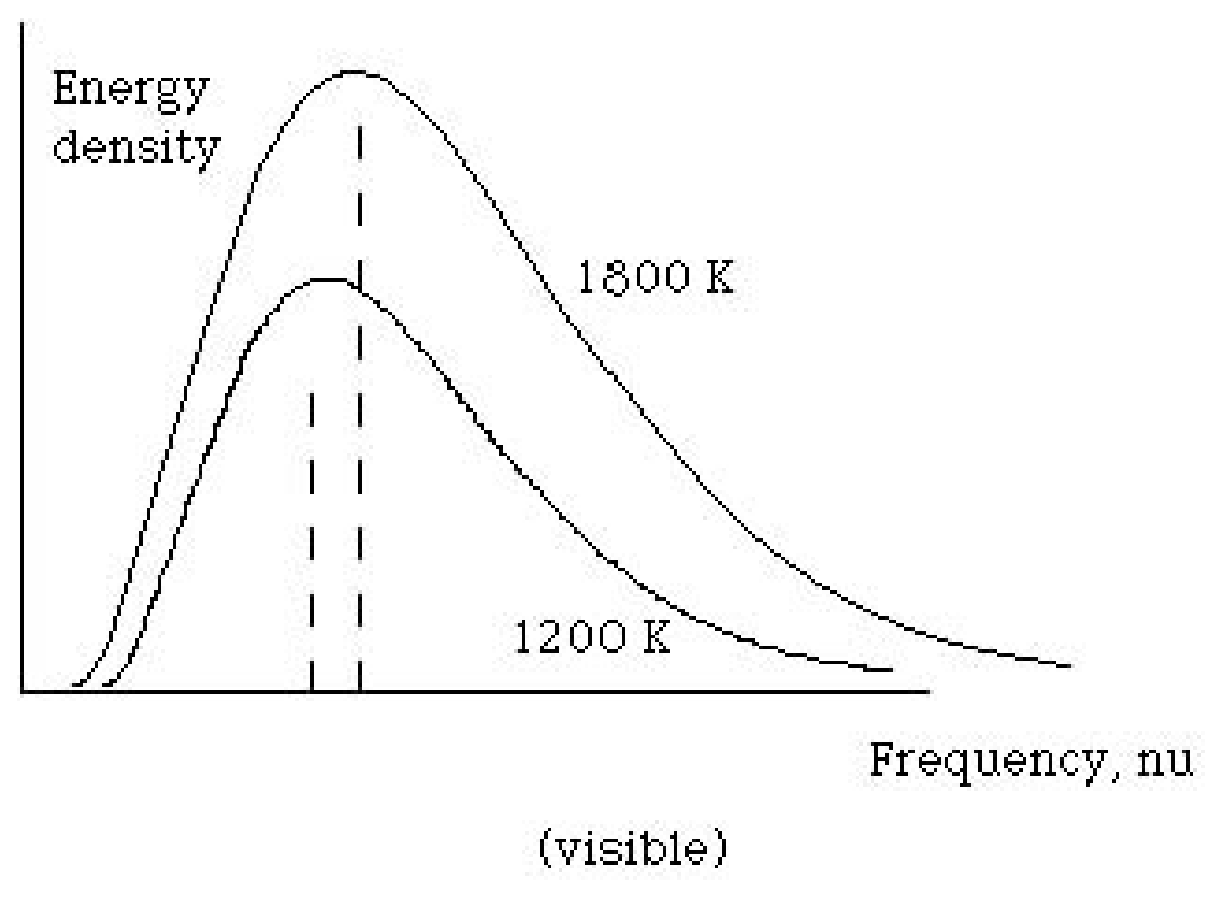
\includegraphics[width=6cm]{Duality/2-3.ps}\\
  \caption{不同温度下的黑体辐射谱}\label{blackbody radiation}
\end{center}
\end{figure}

实验满足以下规律:

\index{Wien's displacement law: 维恩位移定律}

\index{Stefan and Boltzman's law: 斯特番-玻耳兹曼定律}

\begin{enumerate}
    \item {维恩位移定律(Wien's displacement law):$\lambda _{\max } T = 2.898 \times 10^{-3} m K$,即随着温度升高,热辐射峰值向短波高频方向移动。

当孙悟空进入太上老君的炼丹炉的时候,老君通过观察炉口的颜色来判断炉子的温度,刚开始的时候是红色的,然后就是“黄绿青蓝紫”,波长越来越短,炉子的温度越来越高。}

    \item {斯特番-玻耳兹曼定律(Stefan and Boltzman's law):黑体辐射本领$R(T) = \int_0^\infty  {r_b (\lambda ,T)d\lambda } $与热力学温度四次方成正比,即:$R(T) = \sigma T^4 $, $\sigma  = 5.67 \times 10^{ - 8} Js^{ - 1} m^{ - 2} K^{ - 4} $
叫作斯特番-玻耳兹曼常数。}

    \item {为了解释黑体辐射的实验数据,维恩假设气体分子辐射频率只与其速度有关,得到维恩公式:$u_T (\nu ) = \frac{{\alpha \nu ^3 }}{{c^2 }}e^{ - {\raise0.7ex\hbox{${\beta \nu }$} \!\mathord{\left/
 {\vphantom {{\beta \nu } T}}\right.\kern-\nulldelimiterspace}
\!\lower0.7ex\hbox{$T$}}} $,其中:$\alpha$,$\beta$为常量。}

    \item {瑞利根据能量按自由度均分和经典电动力学,得到瑞利-金斯公式(Rayleigh and Jeans law):$u_T (\nu ) = \frac{{8\pi }}{{c^3 }}\nu ^2 k_B T$,显然这个公式对高频无效,因为此时能量密度趋于无限大,这就是著名的紫外灾难。}
\end{enumerate}

\index{Wien's Formula: 维恩公式}

\index{Rayleigh and Jeans law: 瑞利-金斯公式}

\index{Ultraviolet disaster: 紫外灾难}

\begin{figure}[h]
\begin{center}
  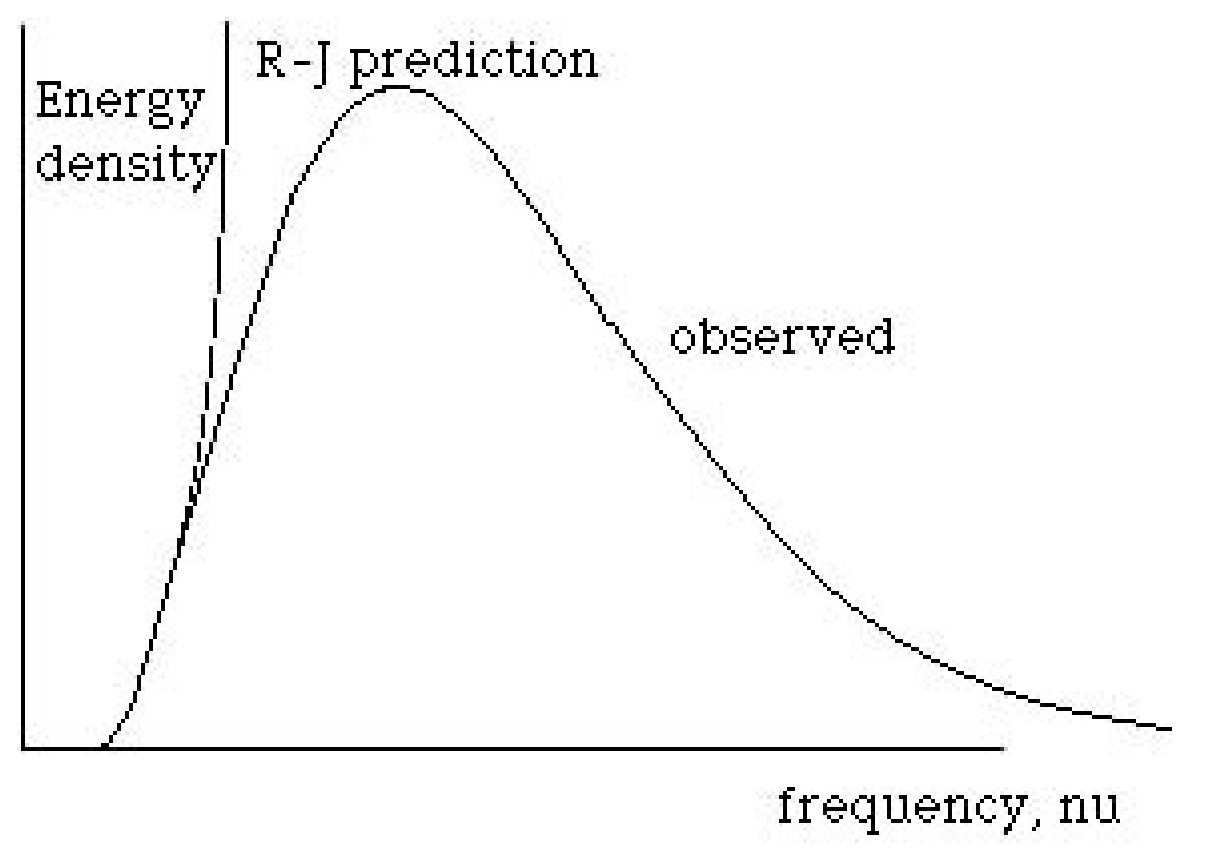
\includegraphics[width=6cm]{Duality/2-4.ps}\\
  \caption{紫外灾难}\label{Rayleigh & Jeans law}
\end{center}
\end{figure}

\subsection{普朗克公式}

\begin{figure}[h]
\begin{center}
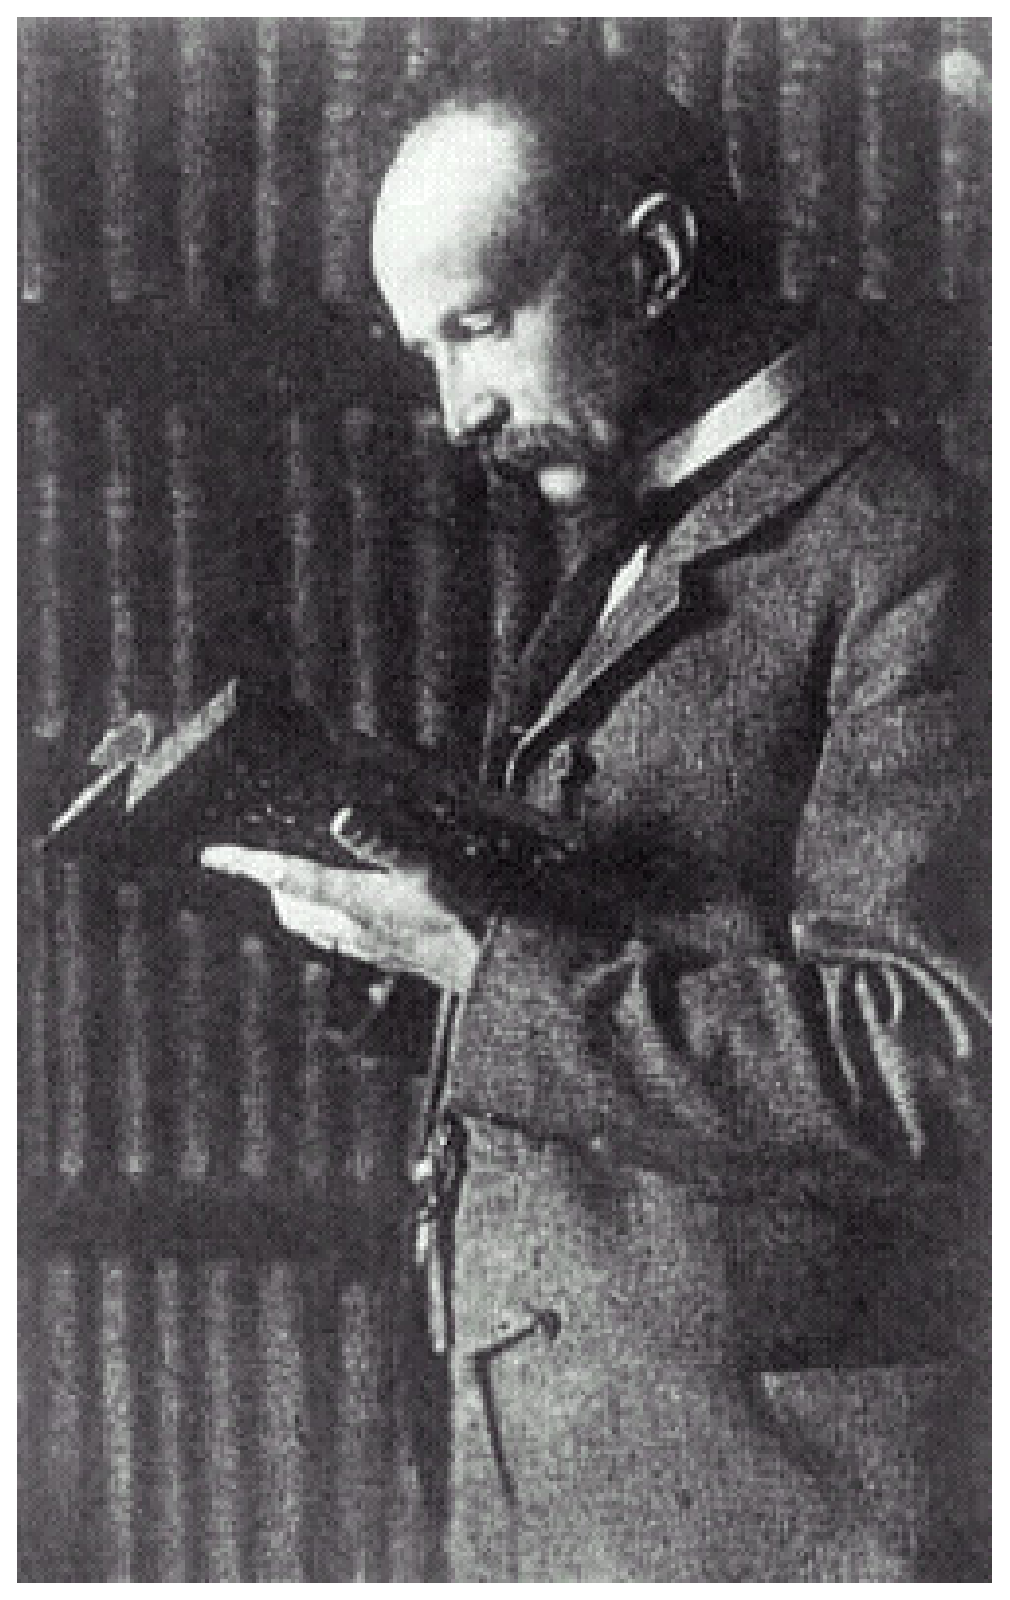
\includegraphics[width=5cm]{Duality/planck.ps}
\caption{普朗克}
\end{center}
\end{figure}

1900年,普朗克(Max Planck)使用内插法,在维恩公式和瑞利-金斯公式的基础上得到了一个新的黑体辐射能量密度公式:

\index{Planck's formula: 普朗克公式}

\begin{equation}\label{planck's law}
u_T (\nu ) = \frac{{8\pi h\nu ^3 }}{{c^3 }} \cdot \frac{1}{{e^{\frac{{h\nu }}{{k_B T}}}  - 1}}
\end{equation}

普朗克公式在整个频率范围与实验结果符合的很好,而维恩公式和瑞利-金斯公式则分别仅在高频和低频下才符合较好。

普朗克并不满足于一个经验公式,很快他得到了公式的理论解释,并提出了量子假说。
即:电磁辐射的能量只能是量子化的,$\varepsilon  = nh\nu $,$n=1,2,3...$,

\begin{equation}
h = 6.626 \times 10^{ - 34} J \cdot s
\end{equation}

$h$被称为普朗克常数,它的单位是“焦耳$\cdot$秒”。对原子物理来说,把它表示为以“电子伏$\cdot$秒”为单位将会更方便,经过简单的计算,或直接查询“WolframAlpha”得到:

\begin{equation}
h = 4.135668 \times 10^{-15} eV \cdot s
\end{equation}

\subsubsection{普朗克公式的推导}

考虑边长为L的立方体,体积内既无电荷也无电流,且有能完全反射的内表面(理想导体),也称为空腔辐射。

回忆电磁波在矩形谐振腔内的电磁振荡\footnote{参考:郭硕鸿《电动力学》,第161页。}。取导体壁的内表面分别为$x=0$和$x=L$,
$y=0$和$y=L$,$z=0$和$z=L$。空腔内电磁波的电场和磁场任一直角分量都满足亥姆霍兹方程:

\begin{equation}
\left( {\nabla ^2  + k^2 } \right)\left\{ {\begin{array}{*{20}c}
   {\mathord{\buildrel{\lower3pt\hbox{$\scriptscriptstyle\rightharpoonup$}}
\over E} }  \\
   {\mathord{\buildrel{\lower3pt\hbox{$\scriptscriptstyle\rightharpoonup$}}
\over B} }  \\
\end{array}} \right\} = 0
\end{equation}

利用分离变量法, 可解出电场分量为:

\index{Separation of variables: 分离变量}

\begin{equation}
\left\{ \begin{array}{l}
 E_x  = A_1 \cos k_x x\sin k_y y\sin k_z z \\
 E_y  = A_2 \sin k_x x\cos k_y y\sin k_z z \\
 E_z  = A_3 \sin k_x x\sin k_y y\cos k_z z \\
 \end{array} \right.
\end{equation}

其中:$k_x  = \frac{{n_x \pi }}{L},k_y  = \frac{{n_y \pi }}{L},k_z =
\frac{{n_z \pi }}{L}$, $n_x ,n_y ,n_z  = 0,1,2,3,...$ ($n_x ,n_y
,n_z$中至少要有两个不为0,否则电场$\hat E = 0$)。

由于立方体内没有电荷分布,$\nabla \cdot \hat E =0$,所以:

\begin{equation}
k_x A_1 + k_y A_2 + k_z A_3 = 0
\end{equation}

因此$A_1$,$A_2$,和$A_3$中有两个是独立的,即对每一组 $(n_x, n_y,
n_z)$ 的本征振荡,有两个独立的偏振模。

考虑波矢空间($\vec k$空间):

\begin{equation}
k^2  = k_x ^2  + k_y ^2  + k_z ^2  = \left( {\frac{\pi }{L}} \right)^2 \left( {n_x ^2  + n_y ^2  + n_z ^2 } \right)
\end{equation}

空腔辐射可能状态(满足驻波条件的状态)坐落在$\left( {\frac{\pi }{L}} \right)$
间距的一系列格点上,即每个状态占据$\left( {\frac{\pi }{L}} \right)^3 $相空间体积。所以$k$半径内总状态数为:

\begin{equation}
N(k) = \frac{1}{8} \cdot \frac{{4\pi k^3 }}{3} \cdot 2 \cdot \left( {\frac{L}{\pi }} \right)^3 = \frac{{\pi k^3 }}{3} \cdot \left( {\frac{L}{\pi }} \right)^3 
\end{equation}

其中:1/8是由于积分仅对第一卦限进行,2是由于每一组$(n_x, n_y, n_z)$的本征振荡,对应两个独立的偏振模。

利用:$k = \frac{{2\pi }}{\lambda } = \frac{{2\pi \nu }}{c}$,得到:

\begin{equation}
N(\nu ) = \frac{{8\pi \nu ^3 L^3 }}{{3c^3 }}
\end{equation}

态密度(Density of states,定义为每单位能量或频率里态的数量)为:

\begin{equation}
g(\nu ) = \frac{1}{V}\frac{{dN(\nu )}}{{d\nu }} = \frac{1}{{L^3 }}\frac{{8\pi \nu ^2 L^3 }}{{c^3 }} = \frac{{8\pi \nu ^2 }}{{c^3 }}
\end{equation}

能量密度为:

\begin{equation}
u_T (\nu ) = g(\nu )\left\langle {\varepsilon (\nu ,T)} \right\rangle
\end{equation}

尖括号表示求热力学平均。

\subsubsection*{对公式的讨论}

\begin{enumerate}
    \item 按照能量均分定理,取$\left\langle {\varepsilon (\nu ,T)} \right\rangle  = k_B T$
(每个自由度均分能量$\frac{{k_B T}}{2}$,电磁场能量密度:$w = \frac{{\varepsilon _0 }}{2}E^2  + \frac{{B^2 }}{{2\mu _0 }}$ ,总平均能量为$k_B T$),于是则得到瑞利-金斯公式:

\begin{equation}\label{rayleigh}
    u_T (\nu ) = \frac{{8\pi }}{{c^3 }}\nu ^2 k_B T
\end{equation}

以上关于瑞利-金斯公式的推导是严格的,紫外灾难不可避免。
这说明在经典物理学的内部(电动力学和统计力学)蕴藏着深刻的矛盾。

(直接计算也可得到:$\left\langle {\varepsilon (\nu ,T)} \right\rangle  = \frac{{\int_0^\infty  {\varepsilon e^{ - {\raise0.7ex\hbox{$\varepsilon $} \!\mathord{\left/
 {\vphantom {\varepsilon  {kT}}}\right.\kern-\nulldelimiterspace}
\!\lower0.7ex\hbox{${kT}$}}} } d\varepsilon }}{{\int_0^\infty  {e^{ - {\raise0.7ex\hbox{$\varepsilon $} \!\mathord{\left/
 {\vphantom {\varepsilon  {kT}}}\right.\kern-\nulldelimiterspace}
\!\lower0.7ex\hbox{${kT}$}}} d\varepsilon } }} = k_B T$
)

\item 利用普朗克量子假说:电磁辐射能量$\varepsilon_n = n h \nu$,$n=0,1,2,3$,…,

\begin{eqnarray*}
\left\langle {\varepsilon (\nu ,T)} \right\rangle &=& \frac{{\sum\limits_n {\varepsilon _n e^{ - {\raise0.7ex\hbox{${\varepsilon _n }$} \!\mathord{\left/
 {\vphantom {{\varepsilon _n } {k_B T}}}\right.\kern-\nulldelimiterspace}
\!\lower0.7ex\hbox{${k_B T}$}}} } }}{{\sum\limits_n {e^{ - {\raise0.7ex\hbox{${\varepsilon _n }$} \!\mathord{\left/
 {\vphantom {{\varepsilon _n } {k_B T}}}\right.\kern-\nulldelimiterspace}
\!\lower0.7ex\hbox{${ k_B T}$}}} } }} = \frac{{\sum\limits_n {nh\nu e^{
- \beta nh\nu } } }}{{\sum\limits_n {e^{ - \beta nh\nu } } }} \\
{} &=& - \left[ {\frac{\partial }{{\partial \beta }}\ln \left( {\sum\nolimits_0^\infty  {e^{ - \beta nh\nu } } } \right)} \right] \\
{} &=& - \left[ {\frac{\partial }{{\partial \beta }}\ln \left( {\frac{1}{{1 - e^{ - \beta h\nu } }}} \right)} \right] \\
{} &= & \frac{\partial
}{{\partial \beta }}\ln \left( {1 - e^{ - \beta h\nu } } \right)
\end{eqnarray*}

这里:$\beta  = \frac{1}{{k_B T}}$,所以:

\begin{equation}
\left\langle {\varepsilon (\nu ,T)} \right\rangle  = \frac{{h\nu e^{ - \beta h\nu } }}{{1 - e^{ - \beta h\nu } }} = \frac{{h\nu }}{{e^{\beta h\nu }  - 1}}
\end{equation}

即得到普朗克公式:

\begin{equation}
u_T (\nu ) = \frac{{8\pi h\nu ^3 }}{{c^3 }} \cdot \frac{1}{{e^{\frac{{h\nu }}{{k_B T}}}  - 1}}\end{equation}

可见,为解释黑体辐射,人们必须引入能量量子化概念:频率为$\nu$的电磁辐射,其能量只能取能量子$h\nu $
的整数倍。这显然与经典物理学矛盾,按经典物理学,能量与振幅的平方成正比,可取从0到无穷大任意值
(对应于维恩公式,但有紫外发散困难)。为了解释自己的公式,普朗克假设能量量子化是由于辐射电磁波的谐振子的能量是量子化的,
电磁辐射场本身的能量是连续的,但它们之间发生能量交换时必须一份、一份地进行,即是量子化的。这种解释看起来有些牵强,
但为了避免“推翻”整个经典物理学体系,也是必然的选择。但后来,光电效应等更多实验表明,辐射场本身也是量子化的。

\index{photon: 光子}

如果我们把$h\nu $理解为光子,
则频率为$\nu$的电磁辐射,对应n个频率为$\nu$ 的光子,
即光强是由光子数目决定的,
辐射场能量分布函数$f$可以看为光子气的密度分布函数$n$。这里我们可以回忆(比较)一下分子运动论中的麦克斯韦速率分布函数:

\begin{equation}
f(v)
= 4\pi \left( {\frac{m}{{2\pi k_B T}}} \right)^{3/2}  \cdot v^2 e^{
- mv^2 /2k_B T} 
\end{equation}

\end{enumerate}

\subsection*{物理常数}

\begin{itemize}
  \item 普朗克常数:$h = 6.626 \times 10^{ - 34} J \cdot s$
  \item 维恩常数:$b = 2.898 \times 10^{-3} m \cdot K$
  \item 斯特番-玻耳兹曼常数:$\sigma  = 5.67 \times 10^{ - 8} Js^{ - 1} m^{ - 2} K^{ - 4}$
  \item 玻尔兹曼常数: $k_B =1.38 \times 10^{-23} J \cdot K^{-1}$
\end{itemize}


\subsection*{阅读与思考}

\begin{itemize}
\item 阅读《天体物理学》(李宗伟等著,高等教育出版社)第2章,``天体物理中的辐射过程'',并写出读书报告。

\item
假设太阳、地球、火星、金星都可看作是绝对黑体,
利用斯特藩-玻尔兹曼定律, 估算金星、地球和火星的表面温度,
这给出了一个讨论温室效应的定量框架。

太阳半径: $R_S  = 6.96 \times 10^5 km$;太阳表面温度: $T_S  = 5780K$;$\sigma  = 5.67 \times 10^{ - 8} Js^{ - 1} m^{ - 2} K^{ - 4} $;水星距离太阳的距离是0.39AU, 火星距离太阳的距离是1.52AU ($1AU = 1.496 \times 10^8 km$)。


解: 太阳总辐射功率: $P = \sigma T^4 4 \pi R_S^2$,
其中只有一部分会照在``地球''上, 比例是: $\frac{\pi R_E^2}{4 \pi
D^2}= \frac{R_E^2}{4 D^2}$, 这里$D$是地球距离太阳的距离(地心到日心).

假设地球表面温度是$T_E$, 地球向外辐射的功率是: $\sigma T_E^4 4 \pi
R_E^2$, 当这个辐射功率和吸收功率相等时, 可估算出地球表面的温度。

\begin{equation*}
\sigma T^4 4 \pi R_S^2 \cdot \frac{R_E^2}{4 D^2} = \sigma T_E^4 4
\pi R_E^2
\end{equation*}

解出:

\begin{equation*}
T_E = T \sqrt{\frac{R_S}{2D}} = 278.77 K
\end{equation*}

这个温度与地球半径($R_E$)无关. 更多结果见下表:

\begin{center}
\begin{tabular}{|l|l|l|l|l|}
  \hline
  % after \\: \hline or \cline{col1-col2} \cline{col3-col4} ...
  {} & 水星 & 金星 & 地球 & 火星 \\
  距离(AU) & 0.39 & 0.73 & 1 & 1.52 \\
  温度(K) & 446 & 326 & 279 & 226 \\
  温度(${}^oC$) & 173 & 53 & 6 & -47 \\
  \hline
\end{tabular}
\end{center}



\textbf{参考}:

\url{http://en.wikipedia.org/wiki/Black_body}


``Engineering the climate'',
\url{http://physicsworld.com/cws/article/print/40222}



``全球变暖之定时炸弹'', 《科学美国人》中文版, 2004年第5期, pp44-53。


\end{itemize}


\subsection*{练习}


\begin{enumerate}

\item 由黑体辐射公式导出维恩位移定律:能量密度极大值所对应的波长$\lambda_m$与温度$T$成反比,即:$\lambda_m T = B$,$B$是一常量,近似计算$B$的数值。

解: 由频率的分布$\int u_T(\nu) d\nu$出发:

\begin{equation*}
\int u_T(\nu)d\nu =\int  \frac{8\pi h
\nu^3}{c^3}\frac{1}{e^{\frac{h\nu}{k_B T}} -1} d \nu
\end{equation*}

变量变换, 把$\nu \to \lambda$, $\lambda = \frac{c}{\nu}$, $d \lambda
= - \frac{c}{\nu^2} d \nu$. 或:$\nu = \frac{c}{\lambda}$, $d\nu = -
\frac{\nu^2}{c} d\lambda=-\frac{c}{\lambda^2}d\lambda$.


\begin{equation*}
\int u_T(\nu) d \nu = \int \frac{8\pi
hc}{\lambda^5}\frac{1}{e^{\frac{hc}{k_B T\lambda}}-1} d\lambda
\end{equation*}

上式中我们把负号``-''略去不写. 现在对新的$\int u_T(\lambda)
d\lambda$中的$u_T(\lambda)$求微分. 极值条件:

\begin{equation*}
\left. {\frac{d u_T(\lambda)}{d\lambda}} \right|_{\lambda =
\lambda_{max}} = 0
\end{equation*}

令: $x = \frac{hc}{k_B T \lambda}$, 上式化简可得:

\begin{equation*}
(5-x)e^x =5
\end{equation*}

这个方程可通过``作图法''求解\footnote{Mathematica:
``FindRoot[5*Exp[x]-x*Exp[x] ==5 , \{x,10\}]''

``解析解'', 网址:

\url{http://www.udel.edu/physics/csaapt/Fall2002/files/analytic-solutions.doc}},
解出: $x \approx 4.97$, 即:

\begin{equation*}
\frac{hc}{k_B T \lambda_{max}} = 4.97
\end{equation*}

即:

\begin{equation*}
    \lambda_{max} T =\frac{hc}{4.97 k_B} = 2.898 \times 10^{-3} m \cdot K
\end{equation*}

值得注意的是如果我们由$\int u_T(\nu) d \nu$出发, 对$u_T(\nu)$求偏导,
即: $\left.{ \frac{d u_T(\nu)}{d \nu}} \right|_{\nu = \nu_{max}}=
0$, 所求出的$\nu_{max}$与$\lambda_{max}$不是一个``颜色'',
即这样定义的$\lambda_{max} \nu_{max} \neq c$.

令$\frac{h\nu}{k_BT}=x$, 由$\left.{ \frac{d u_T(\nu)}{d \nu}}
\right|_{\nu = \nu_{max}}= 0$得到:

\begin{equation*}
    (3-x)e^x = 3
\end{equation*}

利用Mathematica中的FindRoot命令

\begin{verbatim}
    FindRoot[3*Exp[x]-x*Exp[x]==3, {x,10}]
\end{verbatim}

解出: $x \approx 2.82 $, 即:


\begin{equation*}
\frac{h\nu_{max}}{k_BT} = 2.82
\end{equation*}




\end{enumerate}


\section{光的粒子性}

\begin{quotation}
``我们之所以知道光是由粒子组成,是因为我们使用一种非常灵敏的仪器,当光照射这个仪器时,仪器就``嗒''``嗒''``嗒''作响。
如果光变暗了,响声还是那么强,只是响的次数变少了。''\qquad 费曼
\end{quotation}

\subsection{历史回顾}

关于光本性的争论, 持续了很长时间, 牛顿(Newton)认为是粒子,
并解释了光的直线传播, 光的折射现象,
但粒子说无法解释光的干涉和衍射现象\footnote{我们这么说,
牛顿本人未必会同意, 在他看来牛顿环恰恰是``光是粒子''的证据,
但牛顿没法给出计算条纹间距的公式,
而``波动说''可以给出。}。惠更斯(Huygens)认为是机械波, 可以解释:
直线传播、折射、干涉、衍射现象。``光的波动说''因为能解释干涉、衍射现象而稍占上风。

1850年, 麦克斯韦(Maxwell)在法拉第(Faraday)电磁学实验研究基础上,
提出了麦克斯韦方程组, 由麦克斯韦方程组可以推出电磁场波动方程,
电磁波传播速度恰好为光速$c$, 这样, 光学和电磁学就被统一起来,
光波就是电磁波。

\index{Electromagnetic wave: 电磁波}

\begin{eqnarray*}
\nabla  \cdot D = 0,\nabla  \times E =  - \frac{{\partial B}}{{\partial t}},\nabla  \cdot B = 0,\nabla  \times H & = & \frac{{\partial D}}{{\partial t}}  \\
\left( {\nabla ^2  - \frac{1}{{c^2 }}\frac{{\partial ^2 }}{{\partial t^2 }}} \right)\left\{ {\begin{array}{*{20}c}
   {\mathord{\buildrel{\lower3pt\hbox{$\scriptscriptstyle\rightharpoonup$}}
\over E} }  \\
   {\mathord{\buildrel{\lower3pt\hbox{$\scriptscriptstyle\rightharpoonup$}}
\over B} }  \\
\end{array}} \right\} & =  & 0
\end{eqnarray*}

通常我们所说的光就是特定频率的电磁波,
我们可简要地回顾一下电磁波谱的概念\footnote{参考, 杨福家,
《原子物理学》, pp248.}:

\begin{figure}[h]
\begin{center}
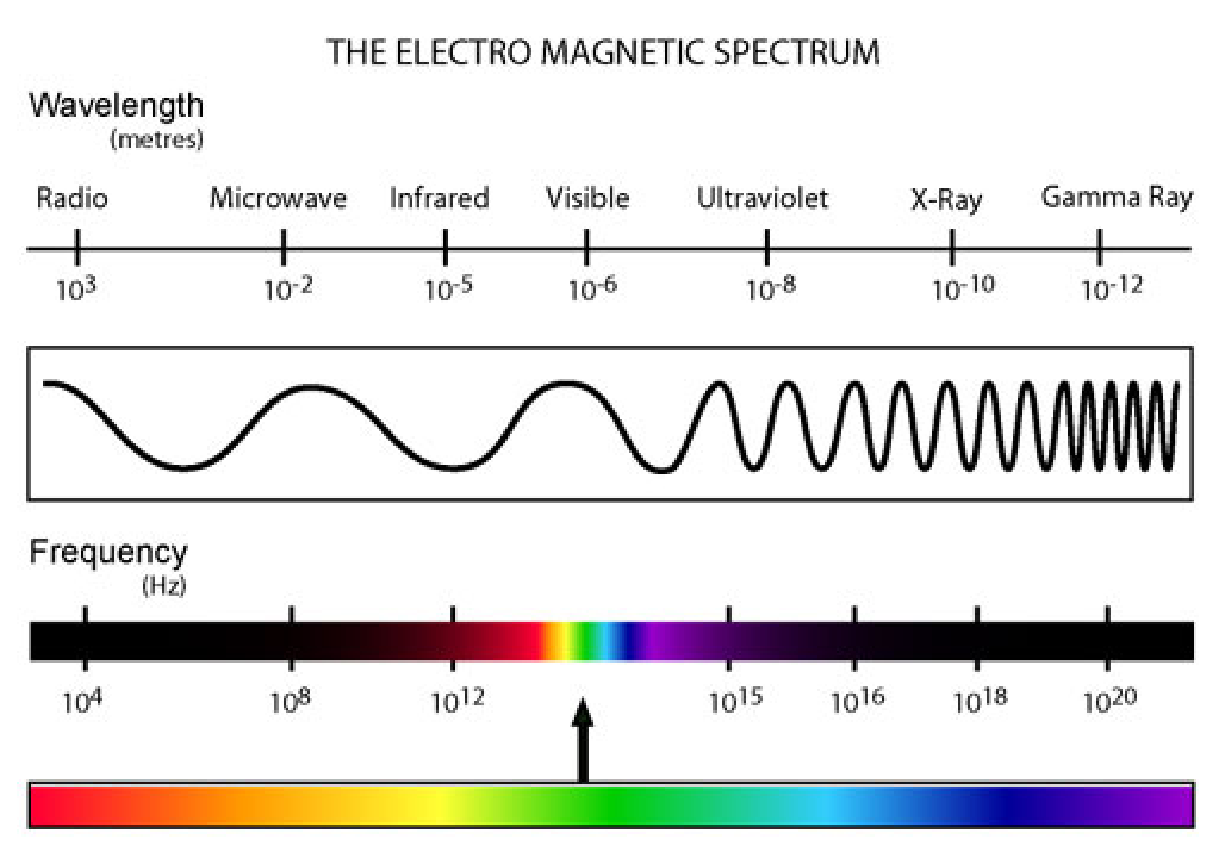
\includegraphics[width=10cm]{Duality/em-spectrum.ps}
\caption{电磁波谱}
\end{center}
\end{figure}

\index{Electromagnetic spectrum: 电磁波谱}

\begin{itemize}
  \item gamma-射线:波长最短(0.01埃左右),能量最高;
  \item X-射线:波长(0.1-10埃),恰好和晶格尺寸吻合,广泛地用于物质结构测定,无损检测,医疗诊断等;能量:$k$eV-$10^5$eV
  \item 紫外(ultraviolet):波长(纳米-百纳米)
  \item 可见光(visible light):波长(几百纳米量级)
  \item 红外(infrared):波长(微米-毫米)
  \item 微波(microwave):波长(毫米,厘米,分米)
  \item 电磁波:波长大于0.1米
\end{itemize}


19世纪末, 为了把Maxwell的电磁理论与Newton的经典力学统一起来,
科学家提出以太学说, 设想光波/电磁波象机械波一样借助某种介质,
即``以太''传播。 以太学说的困难直接导致Einstein提出狭义相对论,
这是量子力学外, 近代物理学又一重大发现。

狭义相对论主要结论:

\index{Special relativity: 狭义相对论}

\begin{enumerate}
    \item 相对论质量:$m = \frac{{m_0 }}{{\sqrt {1 - {\textstyle{{v^2 } \over {c^2 }}}} }}$, $m_0$静止质量。
    \item 动量能量关系:$E = mc^2  = \frac{{m_0 c^2 }}{{\sqrt {1 - {\textstyle{{v^2 } \over {c^2 }}}} }},E^2  = p^2 c^2  + m_0 ^2 c^4 $
    \item 动能:$K = E - m_0 c^2$
\end{enumerate}

\subsection{光电效应}

\index{Hertz's experiment: 赫兹实验}

1887年,赫兹(Hertz)实验证明光波就是电磁波:赫兹用莱顿瓶进行放电实验,
发现了电磁波,电磁波有$\textbf{E}$和$\textbf{B}$的分量,
有散射、干涉、反射等波动特征,传播速度等于光速。赫兹实验验证了Maxwell的理论,并最终判定Newton的光粒子说失败。
但具有讽刺意义的是,在这个``决定性''的实验中,赫兹发现当紫外光(单频)照在负极上时,放电就比较容易发生,
这正是发生光电效应的原因。后来爱因斯坦对光电效应的解释说明:要正确解释光电效应,就必须承认光是粒子。

\begin{figure}[h]
\begin{center}
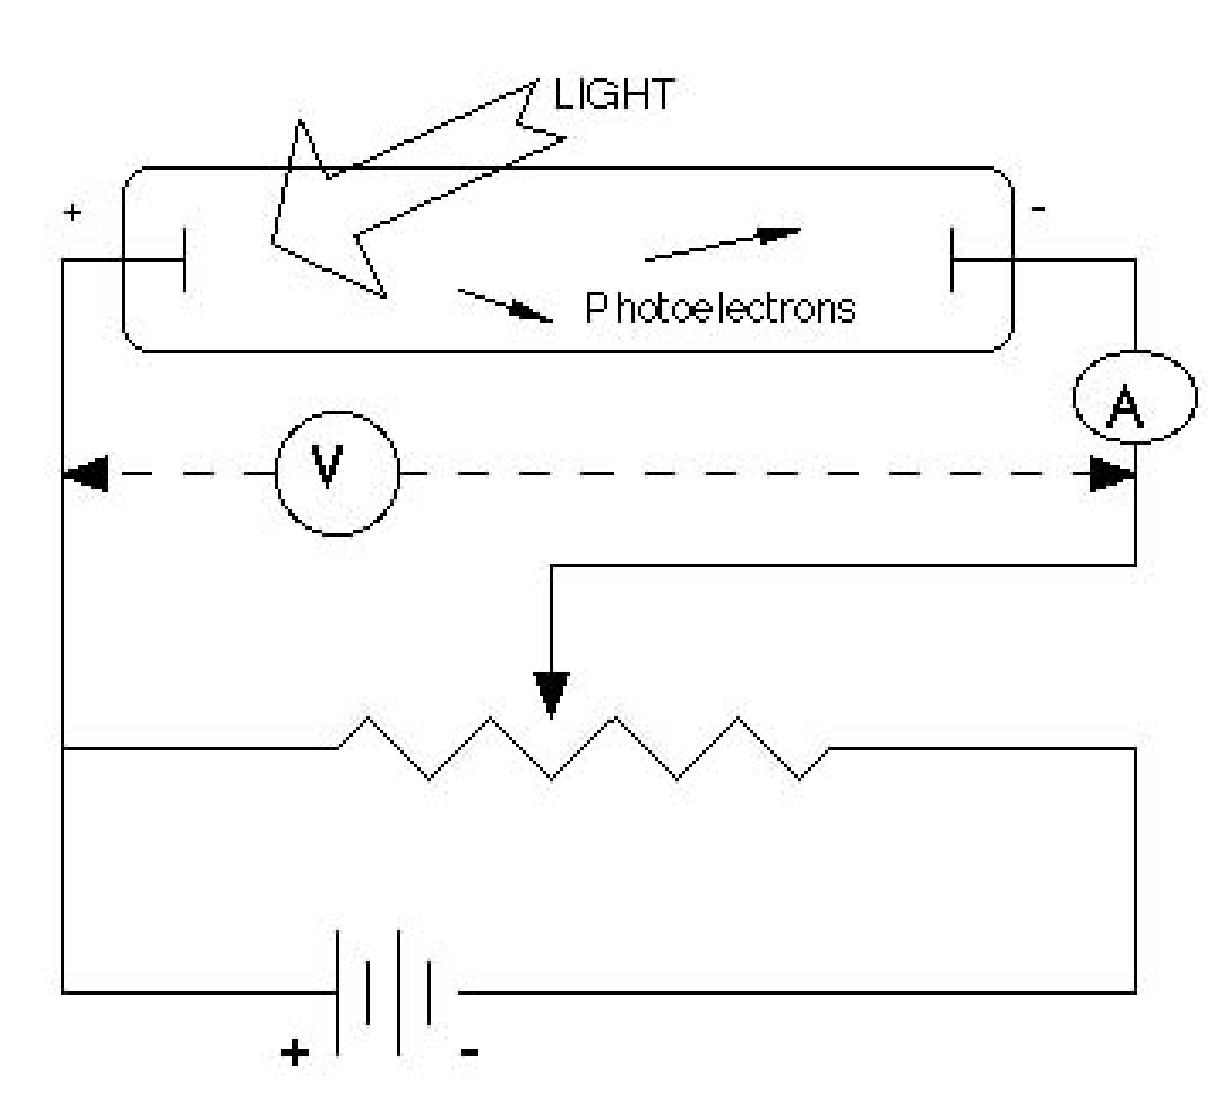
\includegraphics[width=8cm]{Duality/3-1.ps}
\caption{光电效应示意}
\end{center}
\end{figure}

光电效应的实验规律:

\index{Photoelectric effect: 光电效应}

\begin{enumerate}
    \item 饱和电流$I$:随着电压的变大,光电流趋于饱和值(I与单位时间内阴极放出的光电子数成正比)。
饱和电流与光强成正比,或说单位时间内由阴极放出的光电子数与光强成正比。
    \item 存在遏止电压(stopping voltage)$V_0$,遏止电压与光强无关。说明光电子存在最大动能:${\textstyle{1 \over 2}}mv_0 ^2  = eV_0 $。
    \item 存在截止频率(threshold frequency)$\nu _0$,入射光束为单频,改变其频率,发现对应遏止电压随之变化,当入射光低于某频率$\nu _0$时,$V_0$ 减为0,无论光强多大,光电效应不再发生。说明截止频率$\nu _0$与阴极的物性有关。
    \item 弛豫时间$\tau$:弛豫时间与光强无关,光电子几乎在光照瞬间产生,$\tau  < 10^{ - 9} s$。
\end{enumerate}

光的波动理论无法解释光电效应:

(1)按照光的电磁波理论,光强正比于电磁场振幅的平方,电子在变化的电磁场中作受迫振动,
电子振幅足够大时则脱离金属而逸出,类似我们荡秋千时在伙伴的推动下越荡越高的过程。所以光强越大,照射时间越长,
则光电子越容易逸出。但实验表明,光电子是否逸出只与入射光频率有关,而对应弛豫时间很短,无论光强多弱,
整个过程几乎在瞬间完成。

(2)更深入地讨论,如入射光频率与电子振动本征频率接近则发生共振现象,光电子应很快逸出,
但一旦大于此本征频率,电子受迫振动振幅应减小,从而较难逃逸出去,但实验表明一旦入射光超过截止频率,都会有光电效应发生。

\index{photon: 光子}

1905年,受普朗克量子假说启发,爱因斯坦提出光量子假说,正确解释了光电效应:光的能量不象波动理论所想象那样,
是连续分布的(正比于电磁场振幅平方,并分布在空间中),而是集中在一些叫光子(photon)的粒子上,
光子的能量服从普朗克关系:$\varepsilon  = h\nu $。

根据能量守恒, 得到爱因斯坦公式:

\begin{equation}\label{Einstein phtoemission}
   h\nu  = \frac{1}{2}mv_0 ^2  + A = eV_0  + A
\end{equation}

其中:$A = h\nu _0 $,是逸出功(work function),与材料的性质有关。

爱因斯坦对光电效应的解释是:

(1)电磁波能量被集中在光子身上,而不是象波那样散布在空间中,
所以电子可以集中地、一次性地吸收光子能量,所以对应弛豫时间应很短,是瞬间完成的。

(2)所有同频率光子具有相同能量,光强则对应于光子的数目,光强越大,光子数目越多,所以遏止电压与光强无关,
饱和电流与光强成正比。

(3)光子能量与其频率成正比,频率越高,对应光子能量越大,所以光电效应也容易发生,光子能量小于逸出功时,则无法激发光电子。


\subsection{X射线}

光电效应中, 电磁波可以将能量转移给电子并将电子激发出来,
与之相反的过程则是电子撞击物质, 并发出电磁辐射, 即X射线。
X射线辐射:$eV_0  \to h\nu  + e$,可看作是光电效应:$h\nu  + e \to eV_0 $的逆过程。

\index{X-ray: X射线}

1895年,伦琴(Roentgen)发现X射线\footnote{参考杨福家《原子物理学》第246页;}。伦琴是历史上第一个诺贝尔物理奖得主。在19世纪末本来物理学家们认为已经没有什么现象是经典理论无法解释的了,伦琴的发现着实使当时的人们大吃一惊,一种神秘的射线竟然可以穿透人体,并使人身体内部的构造成像。这提示当时的物理学家,求知的过程是没有穷尽的,物理学还远未终结。

在电磁波谱中,X射线在紫外与Gamma射线之间,波长范围一般在0.001nm但1nm,比0.1nm短的称为硬X射线,比0.1nm长的,称软X射线。\footnote{关于电磁波谱:
参考杨福家《原子物理学》第248页;}

\begin{figure}[h]
\begin{center}
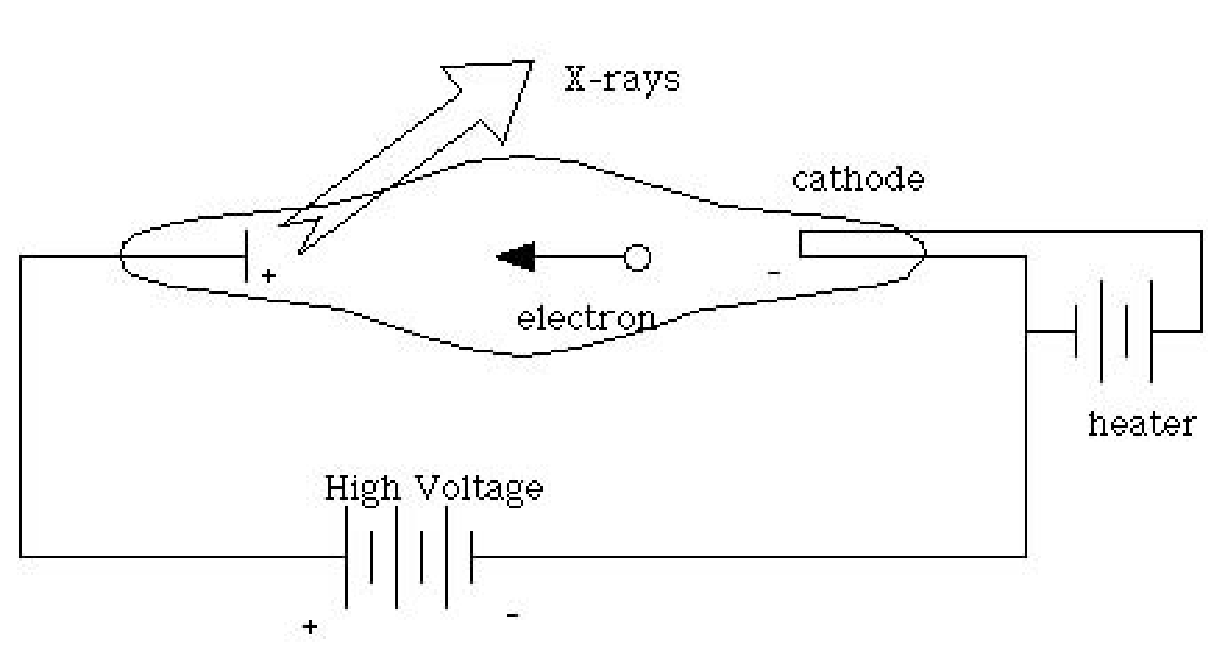
\includegraphics[width=9cm]{Duality/3-2.ps}
\caption{X射线示意}
\end{center}
\end{figure}

根据经典电动力学知识,高速运动电子撞击金属靶,急剧减速,这个过程中必将发生电磁辐射,称为轫致辐射,或刹车辐射。
(轫致辐射的详细理论需要量子电动力学QED的知识)
考虑入射电子与耙原子核之间库仑相互作用,轫致辐射强度反比于入射带电粒子质量平方,正比于靶核电荷的平方
($I \propto \frac{{Z^2 }}{{m_e ^2 }}$),由于带电粒子速度是连续变化的,因此X射线辐射有连续谱的性质。

实验观测到连续谱的形状与靶的材料无关,但存在一个最小波长$\lambda _{\min}$(或最大频率$\nu _{\max }  = \frac{c}{{\lambda _{\min } }}$),其数值仅依赖于加速电压$V_0$,而与耙材料无关。根据普朗克光量子假说:$\varepsilon  = h\nu $,$h\nu _{\max }  = eV_0 $,即最大频率对应于电子动能完全转成辐射能(光子能量)的情况,

\begin{equation}
\lambda _{\min }  = \frac{{ch}}{{eV_0 }}
\end{equation}

这个$\lambda _{\min }$称为量子极限。

\begin{figure}[h]
\begin{center}
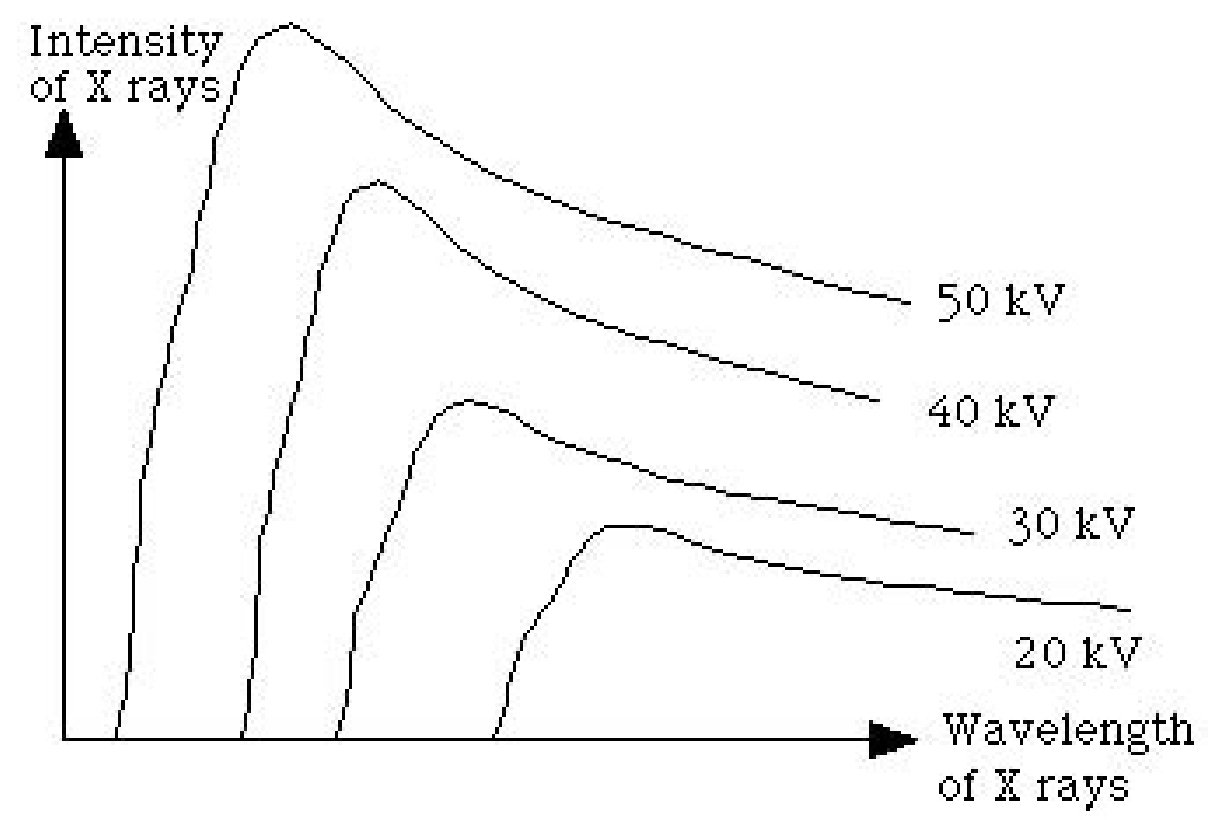
\includegraphics[width=6cm]{Duality/3-3.ps}
\caption{X射线的量子极限}
\end{center}
\end{figure}

实验观察发现,在连续谱上面还存在一些``尖峰'',是特征辐射产生的X射线谱,其对应位置与外加电压无关,
各不同元素的特征X射线谱有类似的结构,但波长位置各不相同,正如指纹可作为人的特征,特征X射线是元素的``指纹''。
特征辐射是经典电动力学所无法解释的,它与原子的内部结构有关系,我们在以后的课程中再给出解释。


\begin{figure}[h]
\begin{center}
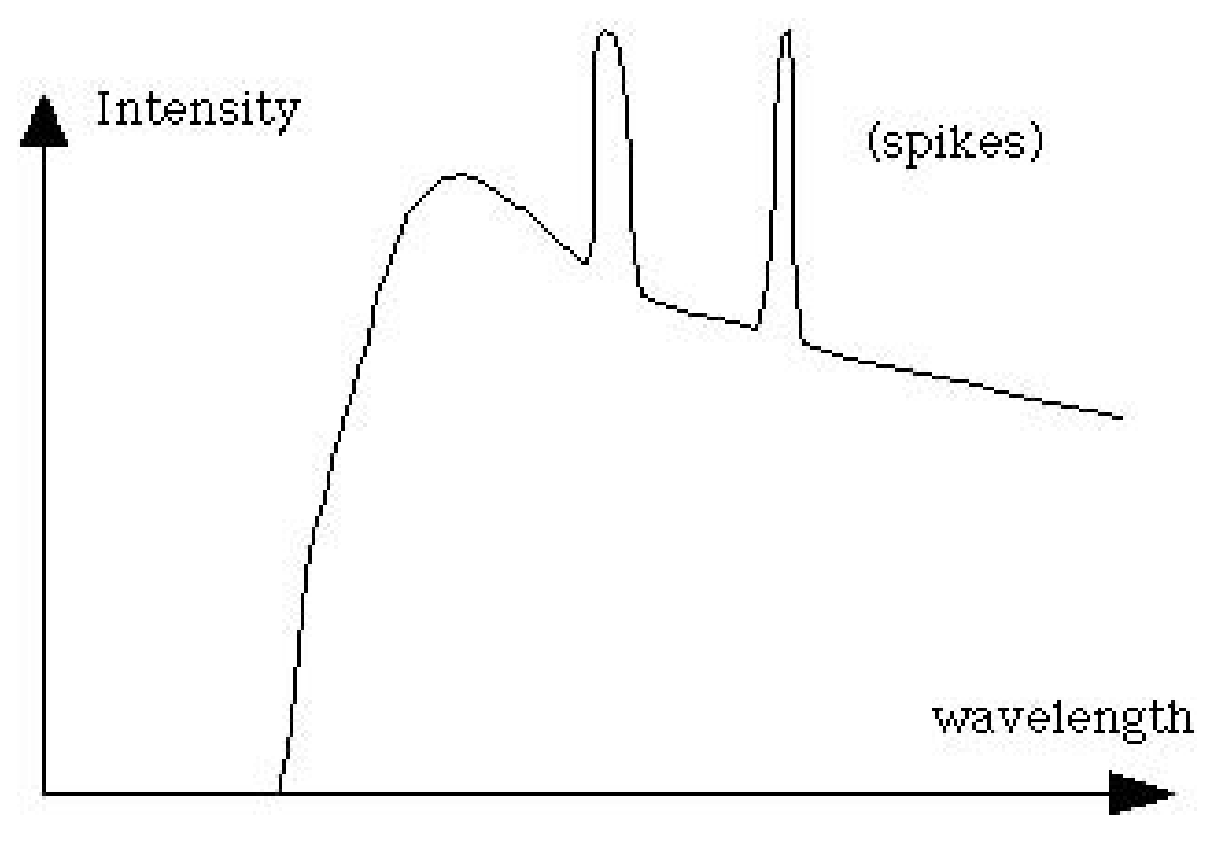
\includegraphics[width=6cm]{Duality/3-4.ps}
\caption{X射线谱的特征辐射}\label{xray-spec}
\end{center}
\end{figure}

特征辐射按辐射的硬度(穿透能力)递减顺序可将特征辐射标记为K、L等系列,并可再细分为$K_\alpha  ,K_\beta  ...,L_\alpha  ,L_\beta  ,...$等谱线\footnote{参考杨福家《原子物理学》第259页;}。

\subsection{X射线衍射}

\index{X-ray diffraction: X射线衍射}

X射线经过大小与其波长类似的狭缝时,将发生衍射现象。对于X射线而言,其波长的数量级为$0.1nm$,很难人工制备这么小尺寸的光栅。
劳厄首先建议用晶体这个天然的光栅用来观察X射线的衍射。

\begin{figure}[htbp]
\begin{center}
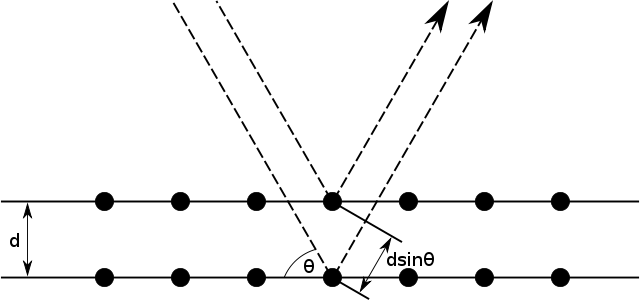
\includegraphics[width=9cm]{Duality/BraggPlaneDiffraction.png}
\caption{布拉格公式}
\label{BraggPlaneDiffraction}
\end{center}
\end{figure}

X射线衍射满足布拉格公式\index{Bragg's formula: 布拉格公式}:

\begin{equation}\label{3-1}
2d \sin \theta = n\lambda, n = 1, 2, ...
\end{equation}

$d$是晶格间的间距,相邻两束光的光程差是$2d \sin \theta$。在布拉格公式中,如图\ref{BraggPlaneDiffraction}, $d$,
$\theta$和$\lambda$都是确定的, 很难有满足此条件的$n$存在,
即很难观察到衍射峰。为克服这个困难,
我们一般用连续的X射线谱(改变$\lambda$)对晶体结构进行分析,
称为\textbf{劳厄法}。
或者我们还可通过转动晶体(改变$\theta$)对晶体结构进行分析,
称为\textbf{旋转晶体法}。 但旋转晶体会涉及到复杂的机械装置,也不方便。

\begin{figure}[htbp]
\begin{center}
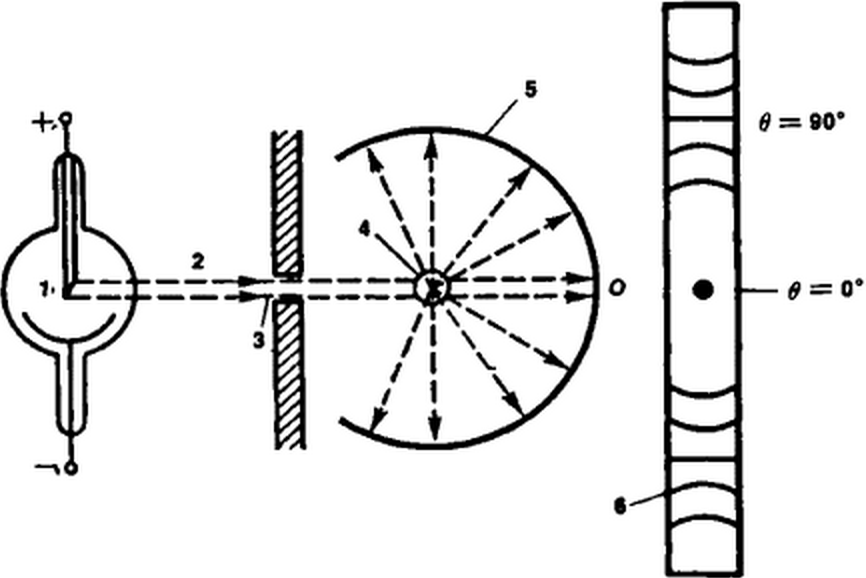
\includegraphics[width=9cm]{Duality/DebyeScherrer.png}
\caption{粉末法示意}
%\label{default}
\end{center}
\end{figure}

如果单色X射线被晶体粉末(或多晶)散射,
由于晶面取向是杂乱无章的,
那些恰好满足布拉格条件的晶面取向(对应特定散射角$\theta$),
将发生相长干涉, 形成衍射条纹, 这种方法称为\textbf{德拜-谢乐法}(或粉末法)。

X射线衍射是重要的结构测量手段,
X射线衍射技术最了不起的发现是导致了DNA双螺旋结构的发现,
从此关于生命现象的研究也建立在原子和分子的水平上了。图\ref{franklin1951}是罗莎琳·富兰克林(Rosalind
Franklin)在1951年得到的,
这是对克里克(Crick)和沃森(Watson)提出的DNA双螺旋结构的直接证据,
图中央由黑点组成的``X形图样''是由于双螺旋结构造成的;
上下两端``弧形图样''是由于碱基每隔$3.4$埃上升一周期造成的。

\begin{figure}[h]
\begin{center}
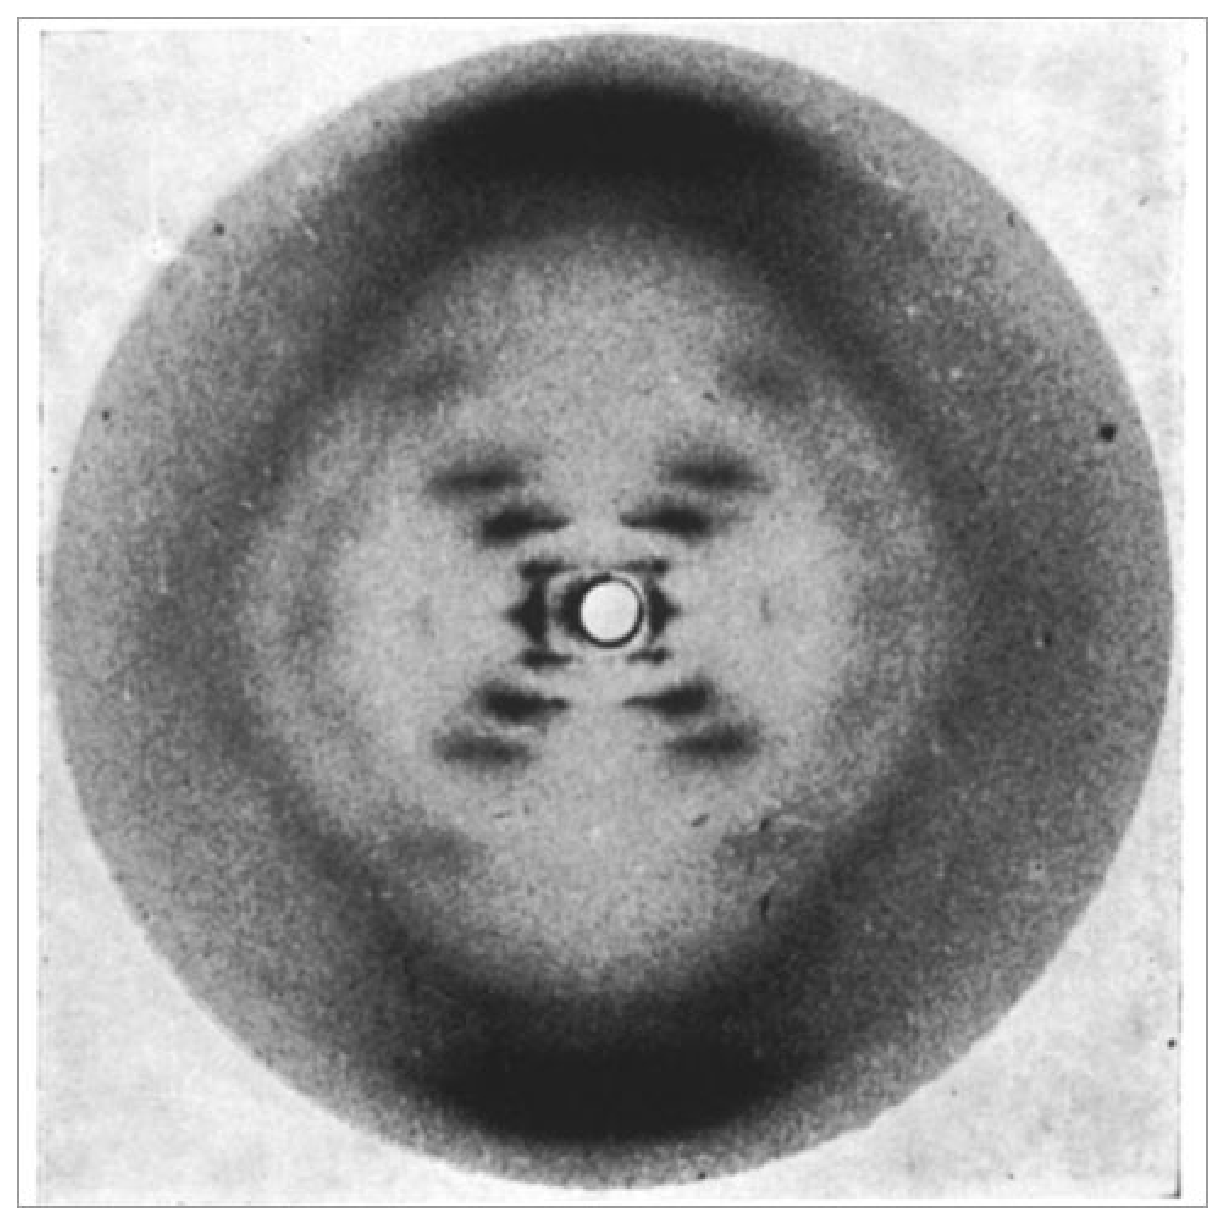
\includegraphics[width=5cm]{Duality/pbs-photo51.ps}
\caption{DNA双螺旋结构的X射线衍射图像}\label{franklin1951}
\end{center}
\end{figure}

\index{DNA Double Helix: DNA双螺旋}

实际上克里克和沃森在构造他们的双螺旋结构的过程中事先就知道了富兰克林和威尔金斯(Wilkins)的X射线衍射数据,
并因此而受益\footnote{``In constructing their model, Watson and
Crick were helped by advance knowledge of X-ray data obtained by
Rosalind Franklin and Maurice Wilkins at King's College London.
These results - and additional data and reasoning supporting the
Cambridge structure - were published in the same issue of Nature.''

参考: ``The Cavendish Laboratory and structural biology'',
\url{http://physicsworld.com/cws/article/print/17020}}。
克里克和沃森的文章,
富兰克林的文章和威尔金斯的文章都发表在自然杂志的同一期(\emph{Nature}
\textbf{171}, 1953)上,
但威尔金斯得到的X射线衍射图像明显没有富兰克林得到的图像清晰。
当克里克, 沃森和威尔金斯在1962年获得诺贝尔生理和医学奖的时候,
富兰克林已经英年早逝了, 她死于1958年, 只有37岁。

目前大多数实验室采用同步辐射加速器作为X射线源。在磁场的作用下高速运动的电子在同步辐射加速器或储存环(Storage ring)里转圈,在电子运动的切线方向会辐射出高质量的同步辐射(synchrotron radiation)。

\begin{figure}[htbp]
\begin{center}
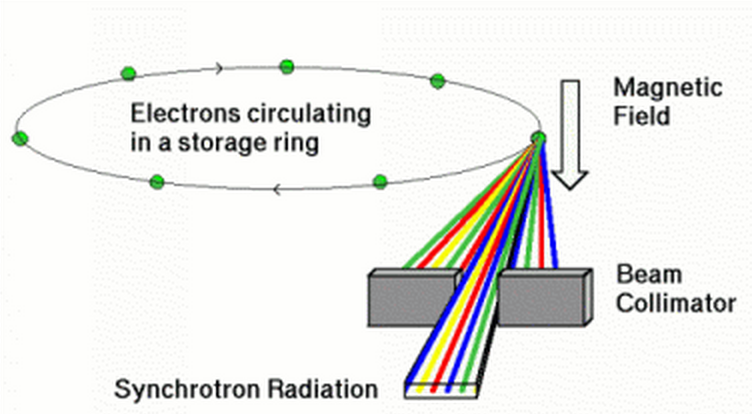
\includegraphics[width=9cm]{Duality/synchrotron.png}
\caption{同步辐射}
%\label{default}
\end{center}
\end{figure}


同步辐射的优点是\footnote{参考杨福家《原子物理学》第266页。关于同步辐射技术, 更多请阅读: 

维基百科词条 Synchrotron radiation:\url{http://en.wikipedia.org/wiki/Synchrotron_radiation}

徐克尊, 《高等原子分子物理学》,科学出版社, 第5.5节。}:

\begin{enumerate}
    \item 功率大;
    \item 能谱宽;
    \item 方向性好。
\end{enumerate}

\begin{figure}[h]
\begin{center}
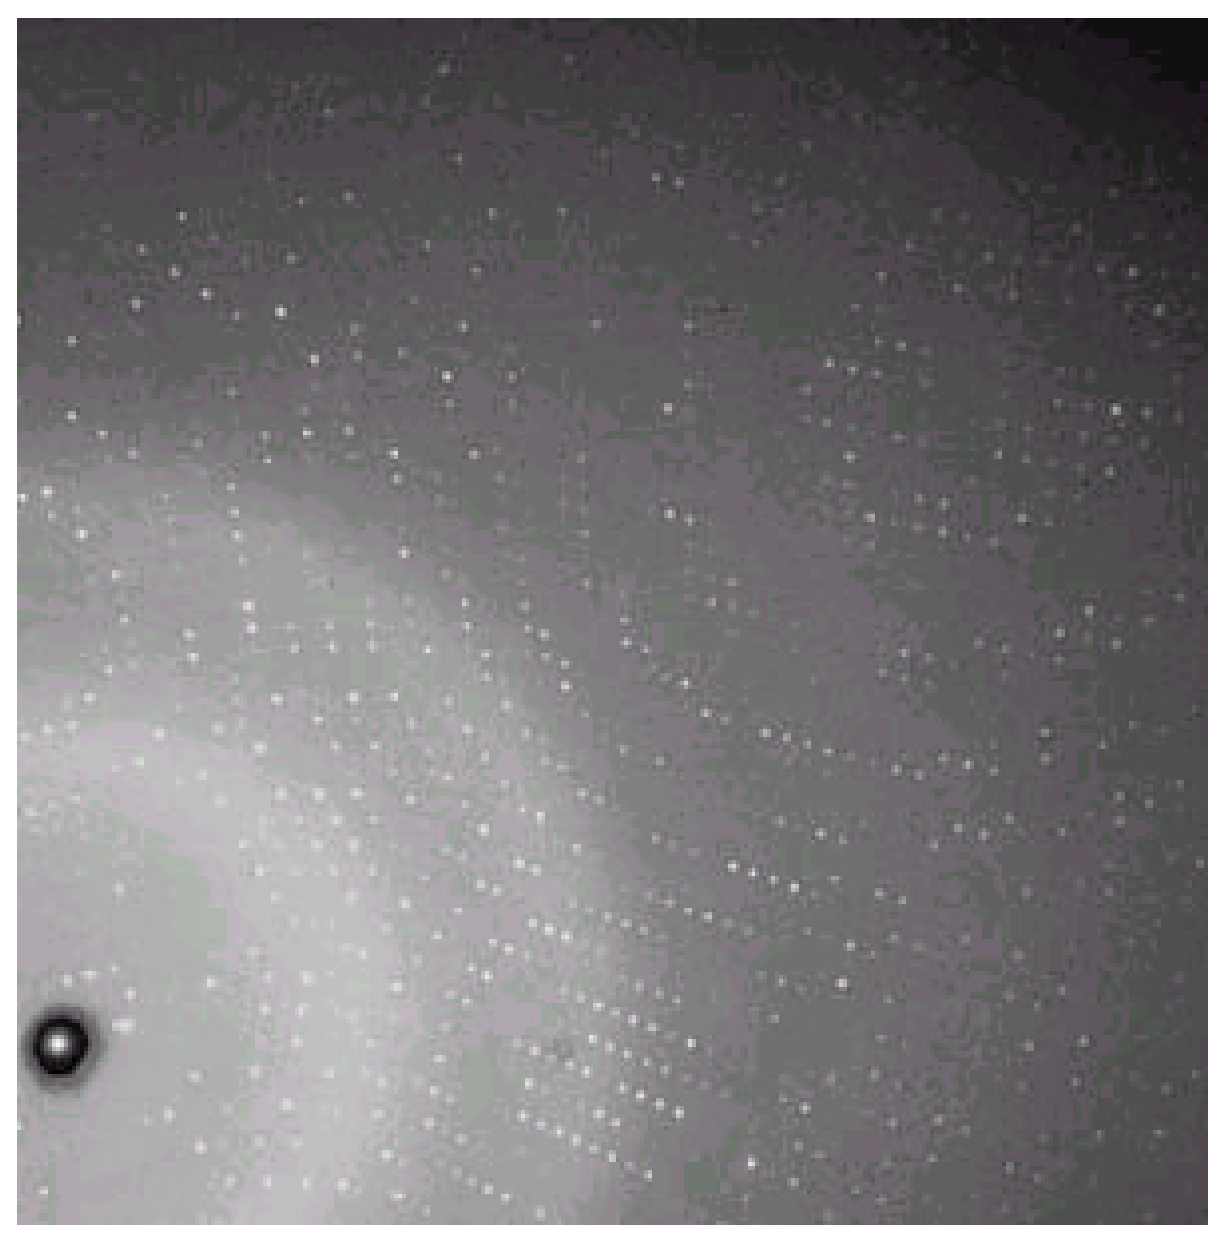
\includegraphics[width=5cm]{Duality/xray.ps}
\caption{蛋白质晶体X射线衍射图像}
\end{center}
\end{figure}


\subsection{康普顿散射}

如果光子是粒子,除具有在空间集中分布的能量外,还应具有在空间集中分布的动量。

爱因斯坦提出光子具有动量\footnote{根据爱因斯坦质能关系: $\varepsilon
= h\nu  = mc^2 ,p = mc = \frac{\varepsilon }{c} = \frac{{h\nu }}{c}
= \frac{h}{\lambda }$}:

\begin{equation}\label{Einstein momentum of photon}
    p = \frac{h}{\lambda }
\end{equation}


\index{Compton scattering: 康普顿散射}

康普顿(Compton)在研究X射线与物质散射的实验中,
发现X射线被轻原子量的物质散射后, 波长有变长的现象。
康普顿散射实验中用的靶的材料是石墨, 由于石墨正好位于周期表的中间,
因此石墨的外层电子束缚的不太结实,
使电子在被高能光子(X射线能量较高)散射前恰好可看作是静止的,
同时又是自由的\footnote{如果使用金属做靶的话,
外层电子是自由的、属于整个金属共有并遵从费米分布。
此时我们可通过康普顿散射轮廓(Compton
Profile)来推测金属内自由电子的动量分布,
并验证其确实满足费米分布。更多, 请阅读: 杨福家, 《原子物理学》,
第三版, pp275-276.}。
假设光子具有动量,碰撞过程中应满足能量与动量守恒,光子与静止电子
之间会发生动量和能量转移, 使光子频率变小,波长变长。

\begin{figure}[h]
\begin{center}
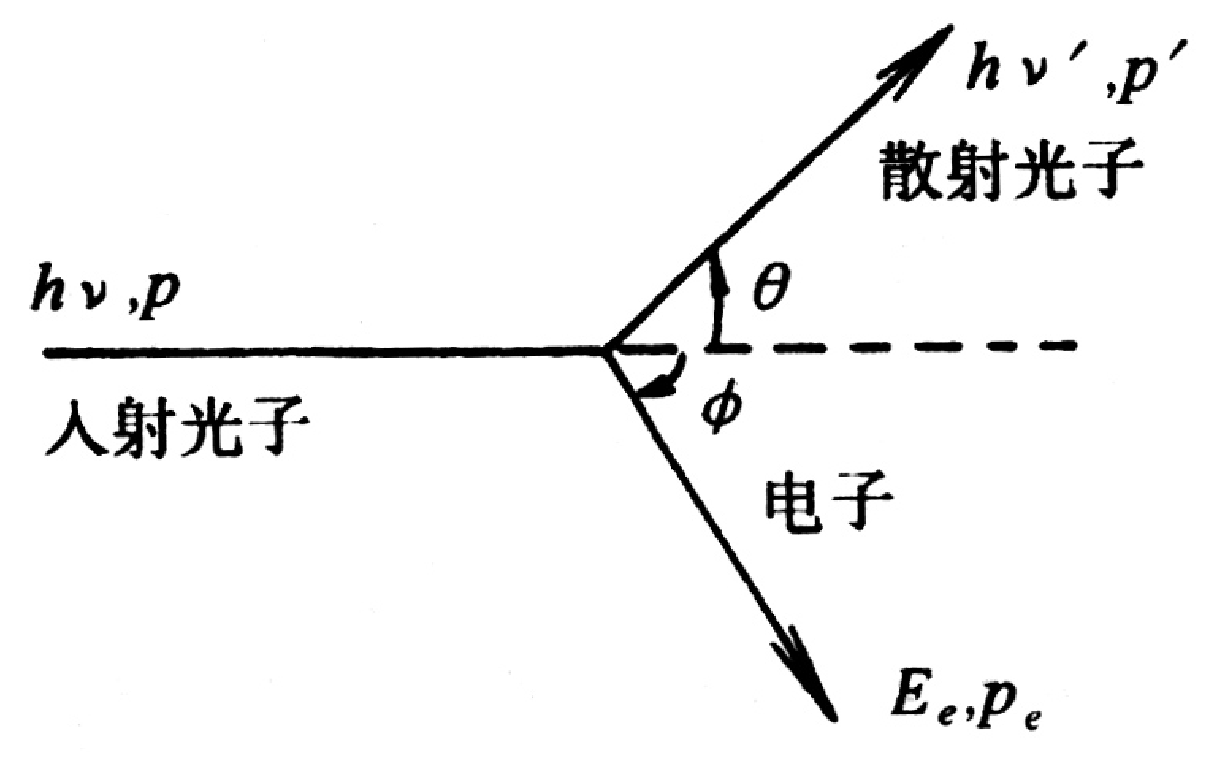
\includegraphics[width=6cm]{Duality/3-5.ps}
\caption{康普顿散射示意}
\end{center}
\end{figure}

碰撞前电子速度很小,视为静止,由于入射光子能量很高(远大于电子在原子中束缚能),所以电子可视为自由电子。


入射光子:$h\nu ,p$;散射光子:$h\nu ',p'$;碰撞后电子:$E_e ,p_e $;$p,p'$夹角$\theta$;$p,p_e $
夹角$\phi$
由于碰撞过程中动量守恒$p = p' + p_e $,碰撞只能发生在同一平面中。

\begin{equation}
\left\{ \begin{array}{l}
 h\nu  + m_e c^2  = h\nu ' + E_e  \\
 p = p' + p_e  \\
 \end{array} \right.
\end{equation}

即:

\begin{equation}
\left\{ \begin{array}{l}
 E_e  = h(\nu  - \nu ') + m_e c^2  \\
 p_e  = p - p' \\
 \end{array} \right.
 \end{equation}

\index{Special relativity: 狭义相对论}

利用相对论能量动量关系:

\begin{equation}
E_e ^2  = p_e ^2 c^2  + m_e ^2 c^4 
\end{equation}

将上式代入化简为:

\begin{equation}
\left[ {h(\nu  - \nu ') + m_e c^2 } \right]^2  = (p - p')^2 c^2  + m_e ^2 c^4 
\label{ComptonScatteringDerivation}
\end{equation}

其中:

\begin{eqnarray*}
(p - p')^2 &=&  \left| p \right|^2  + \left| {p'} \right|^2  -
2\left| p \right| \cdot \left| {p'} \right| \cdot \cos \theta \\
 {} & = & \left( {\frac{{h\nu }}{c}} \right)^2  + \left( {\frac{{h\nu '}}{c}}
\right)^2  - 2\left( {\frac{{h^2 \nu \nu '}}{{c^2 }}} \right)\cos
\theta \\
{} & = & \frac{{h^2 }}{{c^2 }}\left( {\nu ^2  + \nu '^2  - 2\nu \nu
'\cos \theta } \right)
\end{eqnarray*}

公式(\ref{ComptonScatteringDerivation})的左侧(LHS):

\begin{equation*}
\left[ {h(\nu  - \nu ') + m_e c^2 } \right]^2  = h^2 (\nu ^2  + \nu '^2  - 2\nu \nu ') + m_e ^2 c^4  + 2m_e hc^2 (\nu  - \nu ')
\end{equation*}

公式(\ref{ComptonScatteringDerivation})的右侧(RHS):

\begin{equation*}
(p - p')^2 c^2  + m_e ^2 c^4  = h^2 (\nu ^2  + \nu '^2  - 2\nu \nu '\cos \theta ) + m_e ^2 c^4 
\end{equation*}

由“LHS = RHS”化简可得:

\begin{equation*}
 - 2h^2 \nu \nu ' + 2m_e hc^2 (\nu  - \nu ') =  - 2h^2 \nu \nu '\cos \theta
\end{equation*}

即:

\begin{equation*}
m_e c^2 (\nu  - \nu ') = h\nu \nu '(1 - \cos \theta )
\end{equation*}

进一步化简:

\begin{equation*}
h(1 - \cos \theta ) = m{}_ec^2 \left( {\frac{1}{{\nu '}} - \frac{1}{\nu }} \right)
\end{equation*}

最后得到:

\begin{equation*}
\frac{1}{{\nu '}} - \frac{1}{\nu } = \frac{h}{{m_e c^2 }}(1 - \cos \theta )
\end{equation*}

由于$\lambda  = \frac{c}{\nu }$,两边同时乘$c$,得到康普顿散射公式:

\begin{equation}\label{Compton's formula}
    \Delta \lambda  = \lambda ' - \lambda  = \frac{h}{{m_e c}}(1 - \cos \theta )
\end{equation}


\index{Compton wavelength: 康普顿波长}

可定义电子的康普顿波长:

\begin{equation}
\lambda _c  = \frac{h}{{m_e c}} = 2.43 \times 10^{ - 3} nm
\end{equation}

\subsubsection{实验结果}


\begin{figure}[h]
\begin{center}
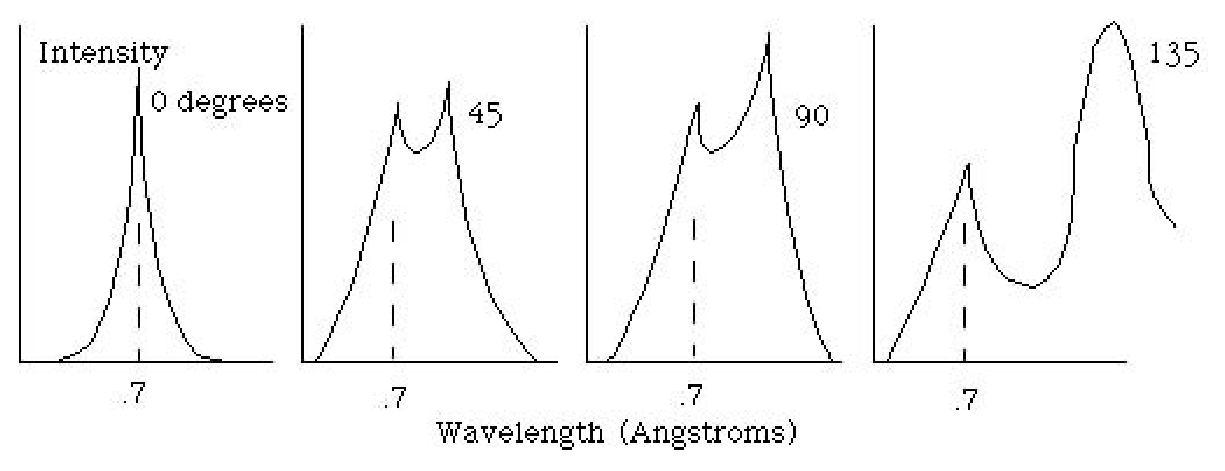
\includegraphics[width=10cm]{Duality/3-6.ps}
\caption{不同角度时的康普顿散射}
\end{center}
\end{figure}

\begin{enumerate}
    \item 根据康普顿散射公式,$\Delta \lambda  = \lambda ' - \lambda  \ge 0$,即散射后波长变长了。
    \item 质子的康普顿波长比电子的小约2000倍,这是为什么我们只考虑了X射线与电子的散射,而没考虑与原子核的散射。
    \item $\Delta \lambda $与入射波波长无关,只决定于散射角$\theta$,$\theta  = 180^o $时最大。\footnote{当$\theta  = 180^o $时,$\Delta \lambda  = 2\frac{h}{{m_e c}} = 0.0049nm$}
    \item 计算中假设电子是自由的,实际上大多数内层电子被束缚很紧,光子同这样的电子碰撞,相当于和整个原子碰撞,
所以动量能量转移很小,所以在散射谱中总存在$\lambda$这条谱线。
\end{enumerate}


\textbf{小结}:黑体辐射、光电效应和康普顿散射表明光具有粒子的特性:
$\varepsilon = h\nu ,p = h/\lambda
$;但光的波动理论早已被干涉、衍射等现象证实,
这样光就具有粒子和波动的双重属性, 这种性质称为:
\textbf{波粒二象性}(Wave-particle duality)。

\index{Wave-particle duality: 波粒二象性}

\subsection*{练习}

\begin{enumerate}
%  \item 普朗克常数($h$)一般用$J \cdot s$为单位表示,现在请换为用$MeV \cdot s$表示。
  \item 频率为$8.5 \times 10^{15} Hz$的光照射在金属表面上,如发射出光电子的动能为$1.7eV$, 求金属的逸出功是多少?(把结果用电子伏$eV$表示)
  \item 要分辨$0.1nm$ 尺度的物质结构,我们需要使用多强的X-射线(用电子伏表示)?
  \item 假设$60W$的灯泡主要发射波长$\lambda = 1000 nm$的光,求每秒发射出的光子数;人的眼睛可分辨,比如最少五个光子的亮光,假设眼睛的瞳孔直径是$0.6cm$,我们最远可在多远看到这只灯泡。
%  \item 某X射线管发出的连续X光谱的最短波长为$0.0124nm$,试问它的工作电压是多少?
  \item 一束波长为$0.54nm$的单色光入射到一组晶面上,
在与入射束偏离$120^o$的方向上产生一级衍射极大,试问该晶面的间距为多大?
  \item 证明:在真空中不可能发生``光子$\rightarrow$正负电子对''过程。
\end{enumerate}


\subsection*{阅读与思考}

\index{photon: 光子}

\begin{itemize}

\item 光是粒子, 某种意义下, 我们的眼睛就是最好的单光子感受器,
有实验表明只需要$1$个光子就可引起一个视杆细胞的兴奋,
$5-9$个光子可使人眼感到一个闪光。阅读:

``Can a Human See a Single Photon?'',
\url{http://www.phys.ncku.edu.tw/mirrors/physicsfaq/Quantum/see_a_photon.html}


\item X射线晶体衍射技术和DNA双螺旋结构的发现, 阅读:


``Double helix: 50 years of DNA'',
\url{http://www.nature.com/nature/dna50/archive.html}


``The Rosalind Franklin Papers'',
\url{http://profiles.nlm.nih.gov/KR/Views/Exhibit/narrative/dna.html}

``James Watson on how he discovered DNA'',
\url{http://www.ted.com/talks/james_watson_on_how_he_discovered_dna.html}(视频)

詹姆斯·沃森,《双螺旋:发现DNA结构的故事》


\end{itemize}


\section{原子结构的玻尔理论}

\begin{quotation}
``当电子从一个定态过渡到另一个定态时,它怎么决定将以什么频率来振动呢?''\qquad 卢瑟福
\end{quotation}

\subsection{原子光谱}

\index{Spectrum: 光谱}

光谱是光的频率和强度分布的关系图, 是研究原子(和分子)结构的重要途径。
如果我们将充有某种原子蒸汽的``真空管''通电, 使之发光,
并测量发出光的光谱,
所测得的便是该元素(该原子)的光谱,即发射光谱(emission spectrum),
谱线是明线。另外一种光谱是吸收光谱(absorption spectrum),
谱线是暗线(低温原子气吸收波长连续分布光源中特定波长光形成)。
同一元素的发射谱线与吸收谱线一一对应。

实验发现相同元素原子谱线相同, 不同元素原子的谱线都不相同,
这些谱线成为辨认不同原子的``指纹''。 利用测量原子光谱的方法,
科学家们发现了很多新元素, 如:He(1862年), Cs(1860年), Rb(1861年)等。

一个关于原子的成功理论必须能解释原子光谱。

\begin{figure}[h]
\begin{center}
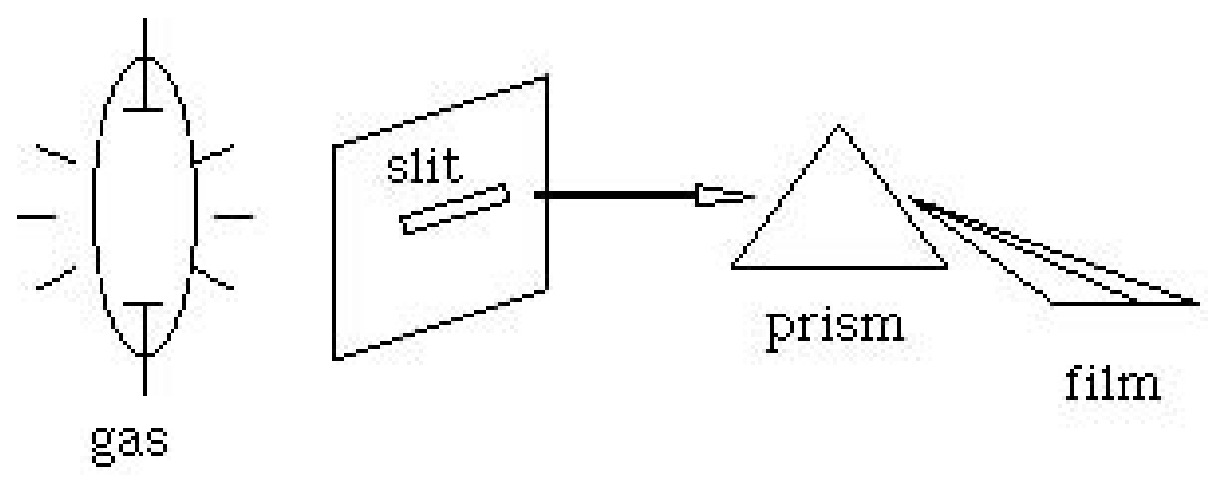
\includegraphics[clip,width=8cm]{BohrModel/4-1.ps}
\caption{原子光谱示意}
\end{center}
\end{figure}

19世纪末, 关于光谱学的实验研究取得了极大进展,
积累了大量实验数据需要整理, 以便从中找出规律, 作出理论解释。
这种情况颇类似于16世纪时第谷积累了大量关于行星运行的数据,
直接导致开普勒在此基础上提出开普勒定律以及后来牛顿建立经典力学理论体系。
目前分子生物学领域测量了各种基因、蛋白质的结构, 并获得大量数据,
但隐藏在这些数据背后的规律还有待我们去发现, 这些规律的发现,
将很可能导致新的科学革命。就象光谱学后来的发展直接导致了玻尔理论及量子力学一样。

\begin{figure}[h]
\begin{center}
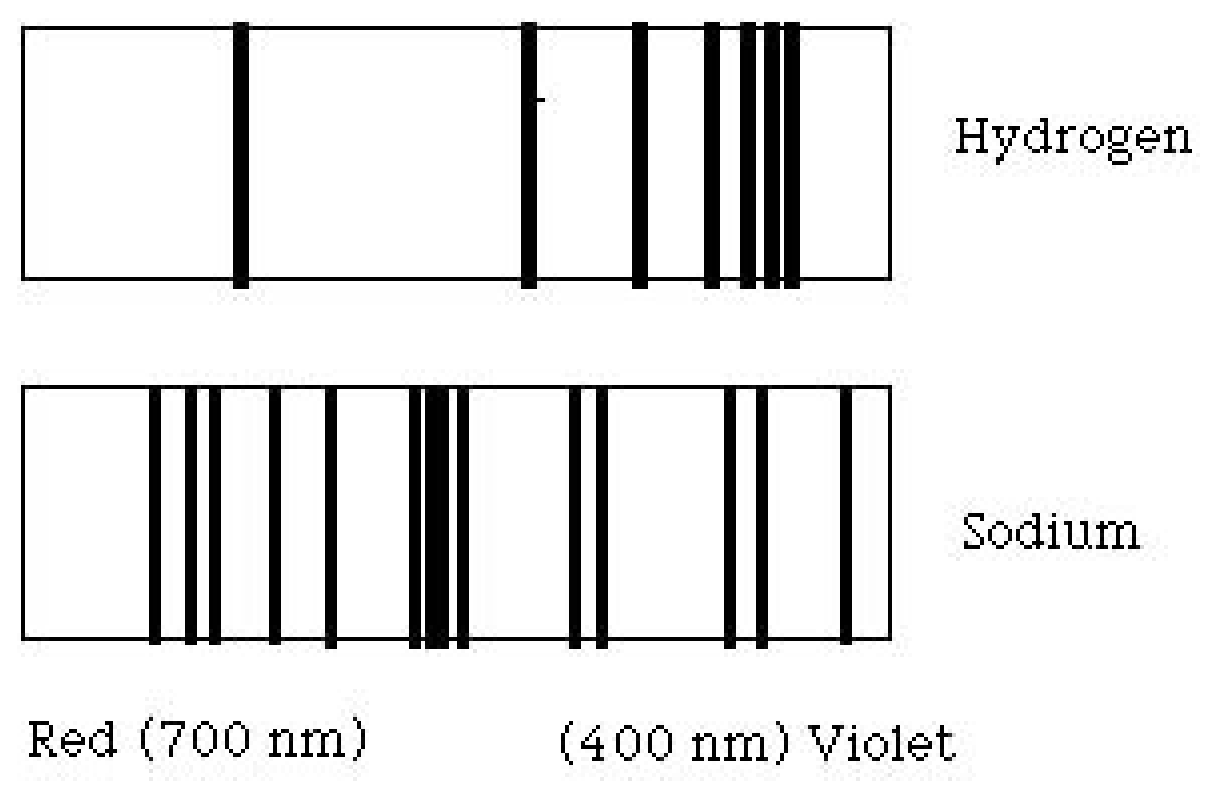
\includegraphics[clip,width=9cm]{BohrModel/4-2.ps}
\caption{氢光谱与钠光谱}
\end{center}
\end{figure}

\subsubsection{氢原子光谱经验规律}

1855年,瑞士中学教师巴尔末(Balmer)发现了关于氢原子光谱的经验公式:

\begin{equation}\label{Balmer's formula}
    \tilde \nu  = \frac{1}{\lambda } = \frac{4}{B}\left( {\frac{1}{{2^2 }} - \frac{1}{{n^2 }}} \right),n = 3,4,5...
\end{equation}

\index{Balmer's formula: 巴尔末公式}

其中:$B=364.56nm$, 这个公式被称为:巴尔末公式(Balmer's formula),
它所描述的这组谱线被称为巴尔末系(Balmer series)。

\index{Balmer series: 巴尔末系}

1889年, 里德堡(Rydberg)提出一个更普遍的方程:

\begin{equation}\label{Rydberg's formula}
    \tilde \nu  = \frac{1}{\lambda } = R_H \left( {\frac{1}{{n^2 }} - \frac{1}{{n'^2 }}} \right) = T(n) - T(n')
\end{equation}

这里:

\begin{equation}
R_H  = \frac{4}{B} = 1.097 \times 10^7 m^{ - 1},
\end{equation}

称为里德堡常数。$T(n)$称为光谱项,$n=1,2,3, ...$,$n' = n + 1,n + 2,n + 3...$

$n=1$时, 赖曼系;$n=2$时, 巴尔末系;$n=3$时, 帕刑系;$n=4$时,
布喇开系;$n=5$时, 普丰特系。

\subsubsection{经典理论的困难}

卢瑟福模型是迈向正确原子模型的关键一步,
但我们使用经典物理学处理卢瑟福模型, 必然得到如下结论:

\index{Rutherford model: 卢瑟福模型}

\begin{enumerate}
    \item 任何作加速运动的带电粒子都要辐射电磁波(即发光),发射电磁波,会使电子能量降低,导致电子轨道不断变小,
并最终落到原子核上,使原子``消失'';
    \item 由于电子能量可以连续变化,所发射电磁波能量也是连续的,原子光谱应是连续的。
由经验和原子半衰期数据知道,原子很稳定,而且原子光谱是线状的,并非连续的。
\end{enumerate}


\subsection{玻尔模型}

\begin{figure}[h]
\begin{center}
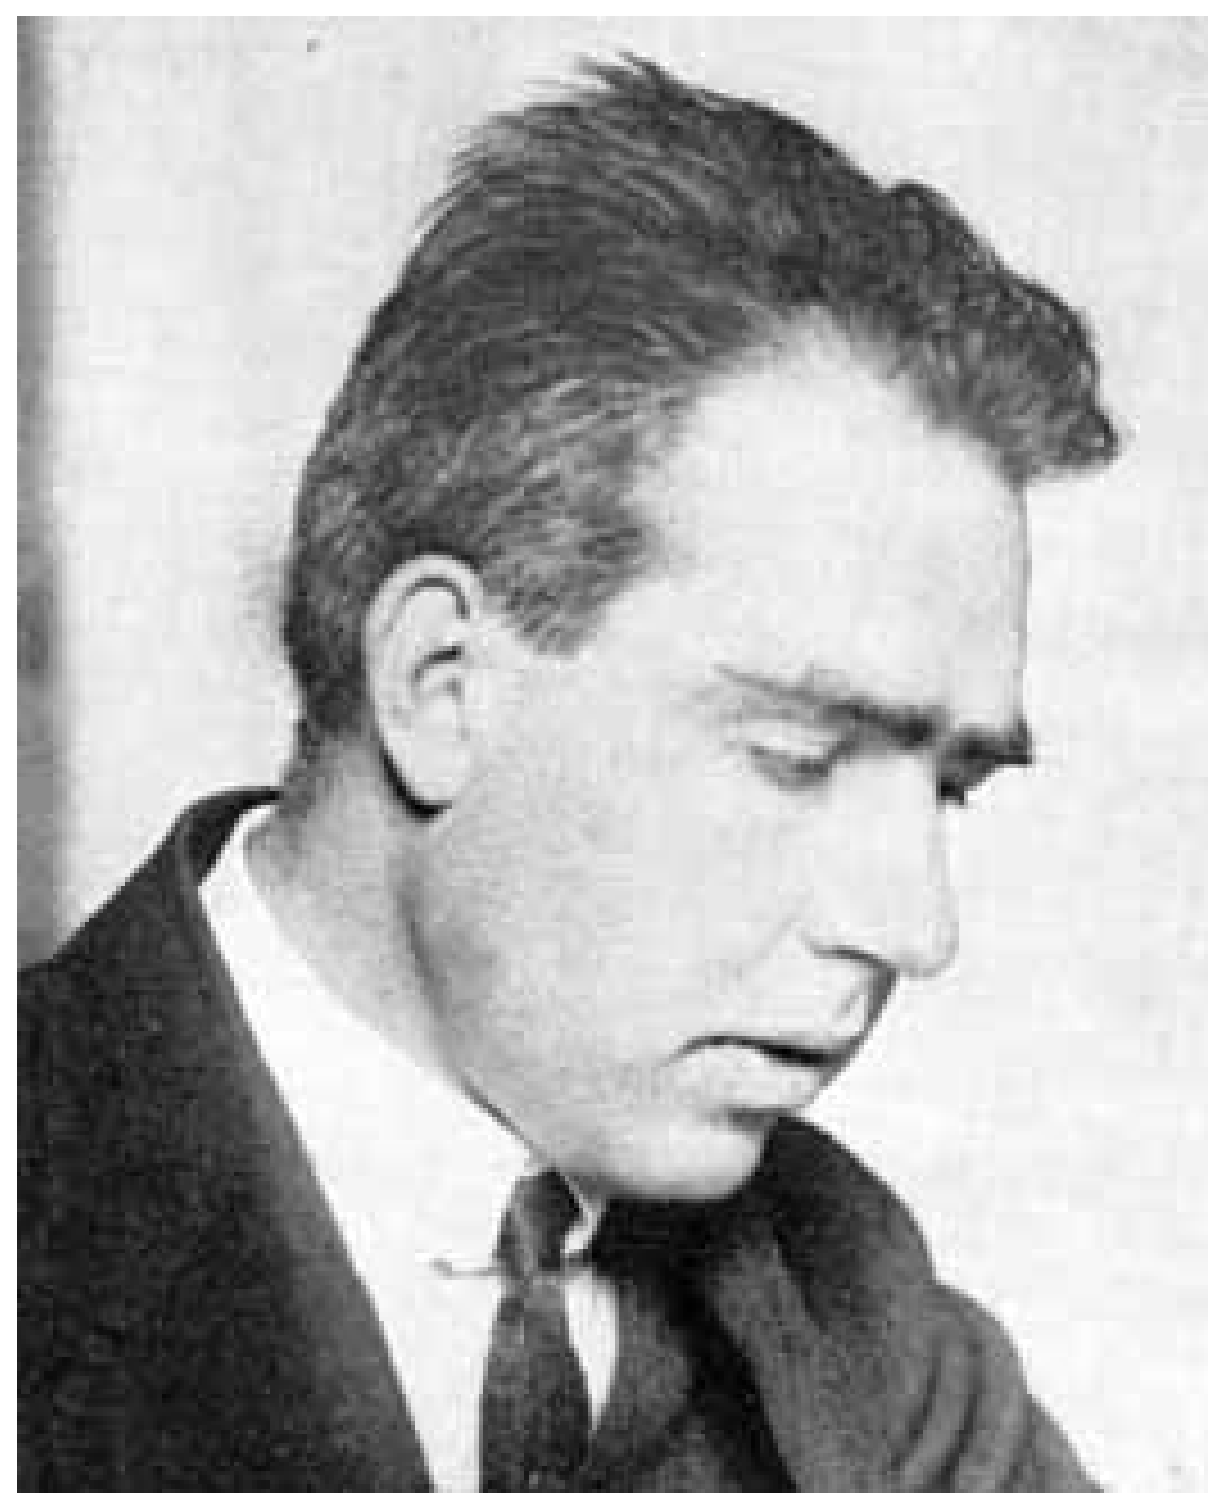
\includegraphics[clip,width=4cm]{BohrModel/bohr.ps}
\caption{玻尔}
\end{center}
\end{figure}

\index{Bohr model: 玻尔模型}

1913年, 玻尔(N. Bohr)正在卢瑟福的实验室工作,
他基于卢瑟福的有核模型(即行星模型, planetary model),
普朗克的量子(quanta)和爱因斯坦的光子(photon)概念解释了氢原子光谱。玻尔的理论基于三个武断的假设,
这三个假设与已有理论——经典力学,经典电磁学——是矛盾的,
而且玻尔也没有真正建立一个全新的理论,
严格意义上的量子力学要在后来才被建立。但玻尔的半截子理论很好地描述了氢原子光谱,
说明他引入的``定态(stationary
state)''等概念对建立量子力学是非常关键的,
这个理论在科学史上被称作旧量子论(Old quantum theory)。

\index{Stationary state: 定态}

\index{Old quantum theory: 旧量子论}

\begin{description}
    \item[定态假设] 原子中存在定态,定态能量取离散值$E_1 ,E_2 ,E_3 ...$。原子在定态时不辐射也不吸收电磁波,玻尔明确指出在氢原子中的定态就是一系列电子围绕原子核的正圆周轨道运动。
    \item[频率条件] 电子在不同定态$E_1 ,E_2 $间可发生跃迁,以发射或吸收特定频率$\nu$光子的形式进行,满足能量守恒,

\begin{equation}
h \nu = E_2 - E_1
\end{equation}

$h$为普郎克常数。频率$\nu$满足:
    
\begin{equation}
\nu  = \frac{{E_2  - E_1 }}{h}.
\end{equation}
    
    \item[角动量量子化] 那么哪些圆周运动才是允许的定态呢,玻尔通过轨道角动量(orbital angular momentum)量子化给出:
    
\begin{equation}
L = n\hbar
\end{equation}

这里:

\begin{equation}
\hbar  = h/2\pi = 1.054572 \times 10^{-34} Js = 6.582119 \times 10^{-16} eV s  
\end{equation}

叫作约化普朗克常数(reduced Planck constant)。

\end{description}

由以上假设不难看出, 玻尔是在经典物理的框架内提出``定态''概念的,
所以玻尔的理论在逻辑上是不自恰的,比如为什么电子可以做圆周运动却不向外辐射电磁波等。要避免这类困难,
必须把``定态''概念重新建立在全新的量子力学基础上。但我们先不管这些,
看看在以上假设下能算出来些什么。

氢原子是由一个电子和一个质子组成,由于$m_e  \ll m_p
$,按单体问题处理。运动方程:

\begin{equation}
F = m_e \frac{{v^2 }}{r} = \frac{1}{{4\pi \varepsilon _0 }}\frac{{e^2 }}{{r^2 }}
\end{equation}

总能量:

\begin{equation}
E = T + V = {\textstyle{1 \over 2}}m_e v^2  - \frac{{e^2 }}{{4\pi \varepsilon _0 r}} =  - \frac{{e^2 }}{{8\pi \varepsilon _0 r}}
\end{equation}

\index{Quantization of angular momentum: 角动量量子化}

利用角动量量子化条件:$L = n\hbar  = m_e vr$:

\begin{equation*}
F = \frac{{e^2 }}{{4\pi \varepsilon _0 r^2 }} = \frac{{(m_e vr)^2 }}{{m_e r^3 }} = \frac{{\left( {n\hbar } \right)^2 }}{{m_e r^3 }}
\end{equation*}

化简可得:

\begin{equation*}
\frac{{e^2 }}{{4\pi \varepsilon _0 }} = \frac{{n^2 \hbar ^2 }}{{m_e r}}
\end{equation*}

最后得到:

\begin{equation}
r_n  = \frac{{4\pi \varepsilon _0 n^2 \hbar ^2 }}{{m_e e^2 }}
\end{equation}

这意味着电子的半径只能取分立的值$r_n$,即量子化的了。这样,能量也将量子化:

\begin{equation}
E_n  =  - \frac{{m_e e^4 }}{{\left( {4\pi \varepsilon _0 } \right)^2  \cdot 2\hbar ^2 n^2 }} =  - \frac{{m_e c^2 }}{2}\left( {\frac{{e^2 }}{{4\pi \varepsilon _0 \hbar c}}} \right)^2  \cdot \frac{1}{{n^2 }}
\end{equation}

\index{Fine-structure constant: 精细结构常数}

定义精细结构常数(fine structure constant, $\alpha$):

\begin{equation}
\alpha = \frac{{e^2 }}{{4\pi \varepsilon _0 \hbar c}} \simeq
\frac{1}{{137}}
\end{equation}

所以:

\begin{equation}
\tilde \nu  = \frac{1}{\lambda } = \frac{\nu }{c} = \frac{1}{{2hc}}m_e \left( {\alpha c} \right)^2 \left( {\frac{1}{{n^2 }} - \frac{1}{{n'^2 }}} \right)
\end{equation}

即里德堡公式。里德堡常数为: 

\begin{equation}
R_H = \frac{1}{{2hc}}m_e \left( {\alpha c} \right)^2
\end{equation}

通过玻尔模型可引入几个重要物理量:

\begin{description}
    \item[第一玻尔半径] n=1时,氢原子半径:
    
\begin{equation}
a_0  = r_1  = \frac{{4\pi \varepsilon _0 \hbar ^2 }}{{m_e e^2 }} \simeq 0.053 nm
\end{equation}

这样电子轨道半径$r_n$可表示为极简单的形式:
    
\begin{equation}
r_n  = a_0 n^2
\end{equation}


    \item[氢原子电离能] 把氢原子电子从基态(n=1)移到无限远($n = \infty $)所需要的能量,
    
\begin{equation}
E_\infty   = \frac{{m_e }}{2}\left( {\alpha c} \right)^2  = 13.6eV
\end{equation}

    \item[玻尔第一速度] 在基态氢原子中电子作圆周运动时的速度:
    
\begin{equation}
v_1  = \frac{\hbar }{{m_e r_1 }} = \frac{\hbar }{{m_e }}\frac{{m_e e^2 }}{{4\pi \varepsilon _0 \hbar ^2 }} = \frac{{e^2 }}{{4\pi \varepsilon _0 \hbar }}\frac{c}{c} = \alpha c
\end{equation}

即电子在氢原子中运动速度为光速的1/137,所以不需考虑相对论效应。

\end{description}

\subsection{玻尔模型的实验验证}

\subsubsection{氢光谱和类氢光谱}

如考虑到原子核不是无穷大情形, $m_e $应由折合质量$\mu  = \frac{{m_e
M}}{{m_e  + M}}$代替, 修正后的里德堡常数应为:

\index{Reduced mass: 折合质量}

\begin{equation}\label{revised Rydberg}
    R_A  = \frac{1}{{2hc}}(\alpha c)^2 \frac{{m_e M}}{{m_e  + M}} = R \cdot \frac{1}{{1 + {\textstyle{{m_e } \over M}}}}
\end{equation}

修正后的里德堡常数与实验测得数据完全吻合。这样,就完全解释了氢光谱的实验数据\footnote{
氢原子里德堡常数的实验值及考虑折合质量修正后的理论值:$R_H =
109677.58 cm^{-1}$, 不考虑折合质量修正时:$R = 109737.315
cm^{-1}$;}。

类氢离子:原子核外只有一个电子的离子, 原子核带正电荷$Ze$
如:He+,Li2+,Be3+等.

对类氢离子, 由于$M \gg m$, 只需考虑电子的单体运动. 电子的总能量是:

\begin{equation*}
E = T+V = \frac{mv^2}{2}- \frac{Ze^2}{4\pi \epsilon_0 r}
\end{equation*}

假设电子作正圆运动, 向心力:

\begin{equation}\label{centripetal force}
\frac{mv^2}{r} = \frac{Ze^2}{4\pi \epsilon_0 r^2}
\end{equation}

考虑``角动量量子化'',

\begin{equation*}
mvr = n \hbar, n=1,2,3,...
\end{equation*}

由公式(\ref{centripetal force}), 可得到:

\begin{equation*}
\frac{n^2 \hbar^2}{mr}=\frac{Ze^2}{4\pi \epsilon_0 }
\end{equation*}

因此轨道半径是``量子化''的,

\begin{equation*}
r_n = \frac{1}{Z}  \frac{4\pi \epsilon_0 n^2 \hbar^2}{me^2}
\end{equation*}

代入到能量的表达式中:

\begin{equation*}
E = - \frac{mv^2}{2} = - \frac{Ze^2}{8 \pi \epsilon_0 r}
\end{equation*}

得到``能量量子化'',

\begin{equation*}
E_n = - Z^2 \frac{me^4}{32 \pi^2 \epsilon_0^2 n^2 \hbar^2}
\end{equation*}

电子速度:

\begin{equation*}
v_n = Z \frac{e^2}{4 \pi \epsilon_0 n \hbar}
\end{equation*}


考虑到精细结构常数:  $\alpha = \frac{e^2}{4\pi \epsilon_0 \hbar c}
$, $r_n$, $E_n$ 和 $v_n$可重新写为:

\begin{eqnarray*}
% \nonumber to remove numbering (before each equation)
  r_n &=& \frac{1}{Z} \cdot \frac{ \hbar}{m c \alpha} \cdot n^2 \\
  E_n &=& - Z^2 \cdot \frac{mc^2}{2} \alpha^2 \cdot \frac{1}{n^2} \\
  v_n &=& Z \cdot c \alpha \cdot \frac{1}{n}
\end{eqnarray*}


即:类氢原子($Z \ne 1$)与氢原子($Z=1$)在轨道半径, 能级,
和速度间的关系是: $r_n = \frac{1}{Z} r(H)_n $, $E_n = Z^2 E(H)_n$,
$v_n = Z v(H)_n$.

``类氢离子''的光谱是:

\begin{equation}\label{Hydrogen-like atoms}
\left( {\frac{1}{\lambda }} \right)_A  = R_A Z^2 \left(
{\frac{1}{{n^2 }} - \frac{1}{{n'^2 }}} \right) = R_A \left(
{\frac{1}{{\left( {{\textstyle{n \over Z}}} \right)^2 }} -
\frac{1}{{\left( {{\textstyle{{n'} \over Z}}} \right)^2 }}} \right)
\end{equation}

这里$n,n',Z$是整数, 但$n/Z,n'/Z$就不一定是整数了,
表现出来类氢光谱的谱线要比氢光谱的要多\footnote{从数学的角度,
只是看起来多而已, 按照数学家的见解, 自然数,
奇数和偶数是一样多的。}。


\subsubsection{夫兰克-赫兹实验}

1914年, 夫兰克-赫兹使用电子流轰击汞蒸汽(mercury vapor),
发现通过真空管的电流随电压增大以$4.9V$为周期, 周期性地变大变小.
说明``汞原子中存在能量为$4.9eV$的量子态''。

\index{Franck-Hertz Experiment: 夫兰克-赫兹实验}

夫兰克-赫兹实验被认为是对“定态”概念和原子的“玻尔模型”的实验证明,
但有趣的是直到夫兰克和赫兹发表了他们的实验结果之后,
他们才知道玻尔模型。文献读少了,这也许是他们的疏忽,但他们在柏林还有一个讨论会(Colloquium),也没用其他人和他们提起玻尔的理论。看来当时的人们根本就不相信看上去复杂无比的原子光谱可能会被某个理论解释,
如果有人声称解释了原子的发射谱线,
当时的物理学家会本能地认为这个理论是错的\footnote{"We had not read it because we were negligent to read the literature
well enough -- and you know how that happens. On the other hand, one
would think that other people would have told us about it. For
instance, we had a colloquium at that time in Berlin at which all
the important papers were discussed. Nobody discussed Bohr's theory.
Why not? The reasons is that fifty years ago, one was so convinced
that nobody would, with the state of knowledge we had at that time,
understand spectral line emission, so that if somebody published a
paper about it, one assumed, Probably it is not right. So we did not
know it."

来源:\url{http://spiff.rit.edu/classes/phys314/lectures/fh/fh.html}}。

\begin{figure}[h]
\begin{center}
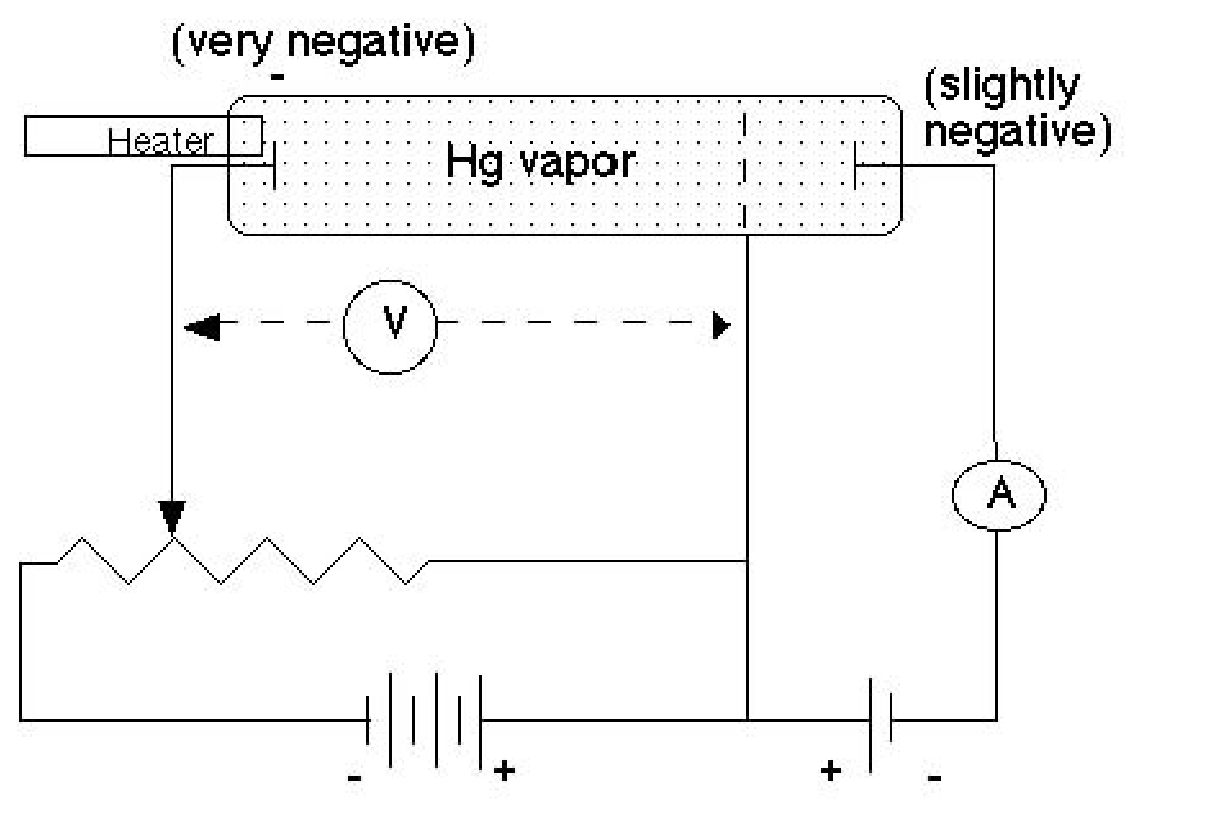
\includegraphics[clip,width=7cm]{BohrModel/4-3.ps}
\caption{夫兰克-赫兹实验示意}\label{Feank-Hertz_experiment_device}
\end{center}
\end{figure}

夫兰克-赫兹实验的装置如图\ref{Feank-Hertz_experiment_device}所示.
水银(汞,Hg)蒸汽被放在真空管内, 电子从阴极射出后, 被电势$V$加速,
然后到达阳极, 阳极是栅栏状的, 阳极后面还有一个微弱的反向电压,
反向电压比加速电压($V$)弱的多,
再后面是个集电极(类似真空三极管,发射极,基极和集电极)。

\begin{figure}[h]
\begin{center}
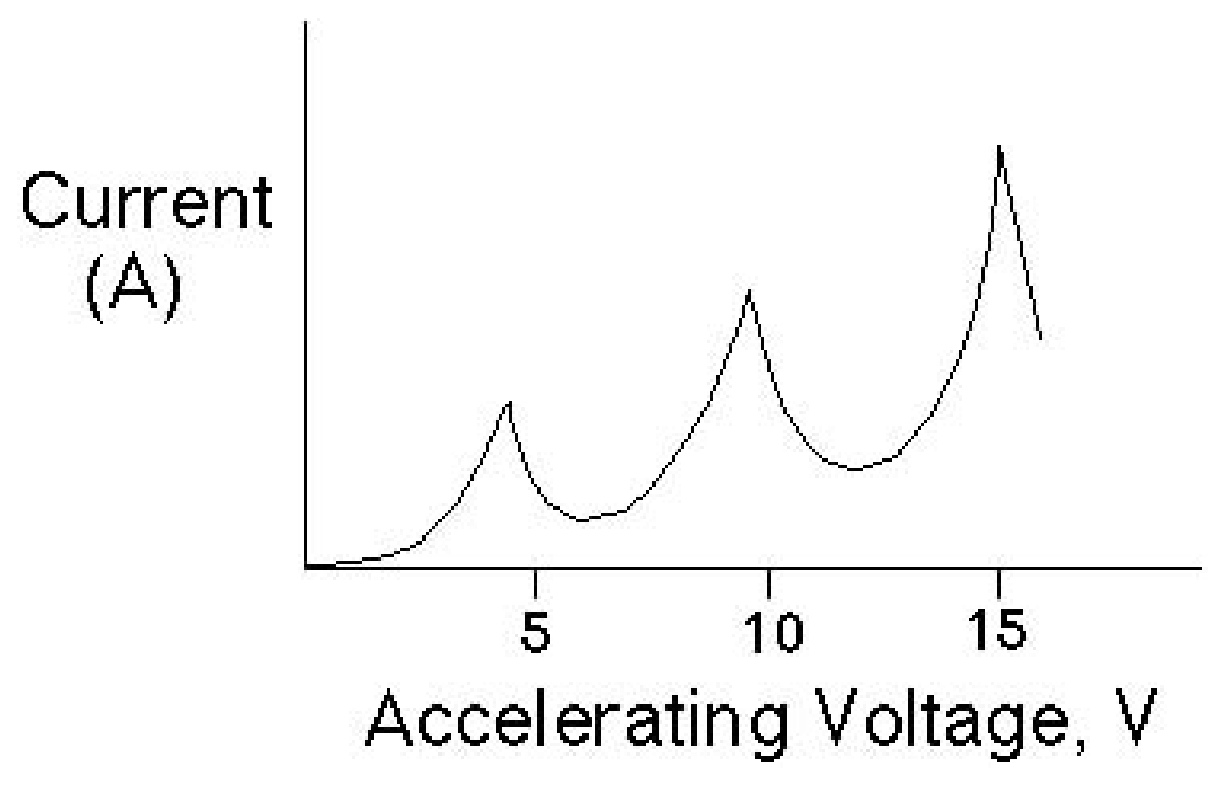
\includegraphics[clip,width=6cm]{BohrModel/4-4.ps}
\caption{夫兰克-赫兹实验:电流随电压增大以4.9V为周期,周期性地变大变小}\label{Frank-Hertz_experiment_result}
\end{center}
\end{figure}

实验测量的是加速电压($V$)和通过集电极电流($I$)之间的关系,实验结果见图\ref{Frank-Hertz_experiment_result}.
可见这里存在一个约$4.9$伏的周期,每$4.9$伏周期,集电极电流会周期性的变大,达到峰值,然后陡峭地变小。

\index{Stationary state: 定态}

这$4.9$伏的周期性可被玻尔模型所解释. 根据玻尔模型,
原子中存在一系列的定态(stationary states),
当原子由一个定态跃迁到另一定态时, 可相应地吸收或放出一个光子,
并满足频率关系(frequency relation):$h\nu =E_2 - E_1$.
$4.9$伏的周期性说明在汞原子的第一激发态与基态间能量差是$4.9eV$。

当加速电压处于$0-4.9$伏区间时, 电子将获得$0-4.9eV$的动能,
电子可能与汞原子发生弹性碰撞或非弹性碰撞,
如发生非弹性碰撞电子将损失部分能量, 而汞原子将获得部分能量.
但根据玻尔模型, 小于$4.9eV$的能量是不足以使汞原子发生跃迁的,
因此只能发生弹性散射, 电子在弹性散射的过程中并不损失能量,
因此当电子达到阳极时具有大于$0$的动能, 可以克服反向电压达到集电极,
因此表现为有电流, 并且随着加速电压的增大, 电流也相应增大.

当加速电压正好为$4.9$伏时, 电子具有$4.9eV$的动能,
可与汞原子发生非弹性散射, 汞原子被激发到激发态,
电子损失$4.9eV$后动能为0, 无法克服反向电压, 因此表现为电流急剧下跌。

当加速电压达到两倍$4.9$伏时,
则有可能发生两次电子与汞原子的非弹性散射,
因此将出现第二个峰。如果继续增大加速电压,
还可能出现更多的峰。如果电子能量大到足以把汞原子激发到更高激发态的能量,
则可以出现不是$4.9$伏周期的峰。

观察夫兰克-赫兹实验的实验曲线, 另一特征是电流波谷取值是逐渐变大的,
这可以解释为总有部分电子未发生与汞原子的非弹性散射就到达了阳极,
从而肯定会到达集电极。发生$N+1$次非弹性散射的几率要小于只发生$N$次非弹性散射的几率,
因此随着加速电压的增大会有更多的电子以非零动能到达阳极,
体现为电流波谷取值越来越高。

还可以考虑更多因素, 比如无规则热运动对夫兰克-赫兹实验曲线的影响,
将使曲线更加圆滑等等。但这些已经属于实验中不太重要的细节了。

1925年夫兰克和赫兹因夫兰克-赫兹实验共同获得诺贝尔物理学奖。


\subsubsection{X射线特征辐射}

如图~\ref{xray-spec},X射线谱由连续谱(continuous
spectrum)和特征谱(characteristic spectrum)两部分组成。
1913年,莫塞莱(Moseley)在测量了从铝到金共38种元素的光谱后发现X射线特征频率的平方根对原子序数$Z$作图,
满足线形关系:

\begin{equation}
\nu _{K_\alpha  }  = 0.248 \times 10^{16} (Z - 1)^2 Hz
\end{equation}

\index{Moseley's law: 莫塞莱定律}

\begin{figure}[h]
\begin{center}
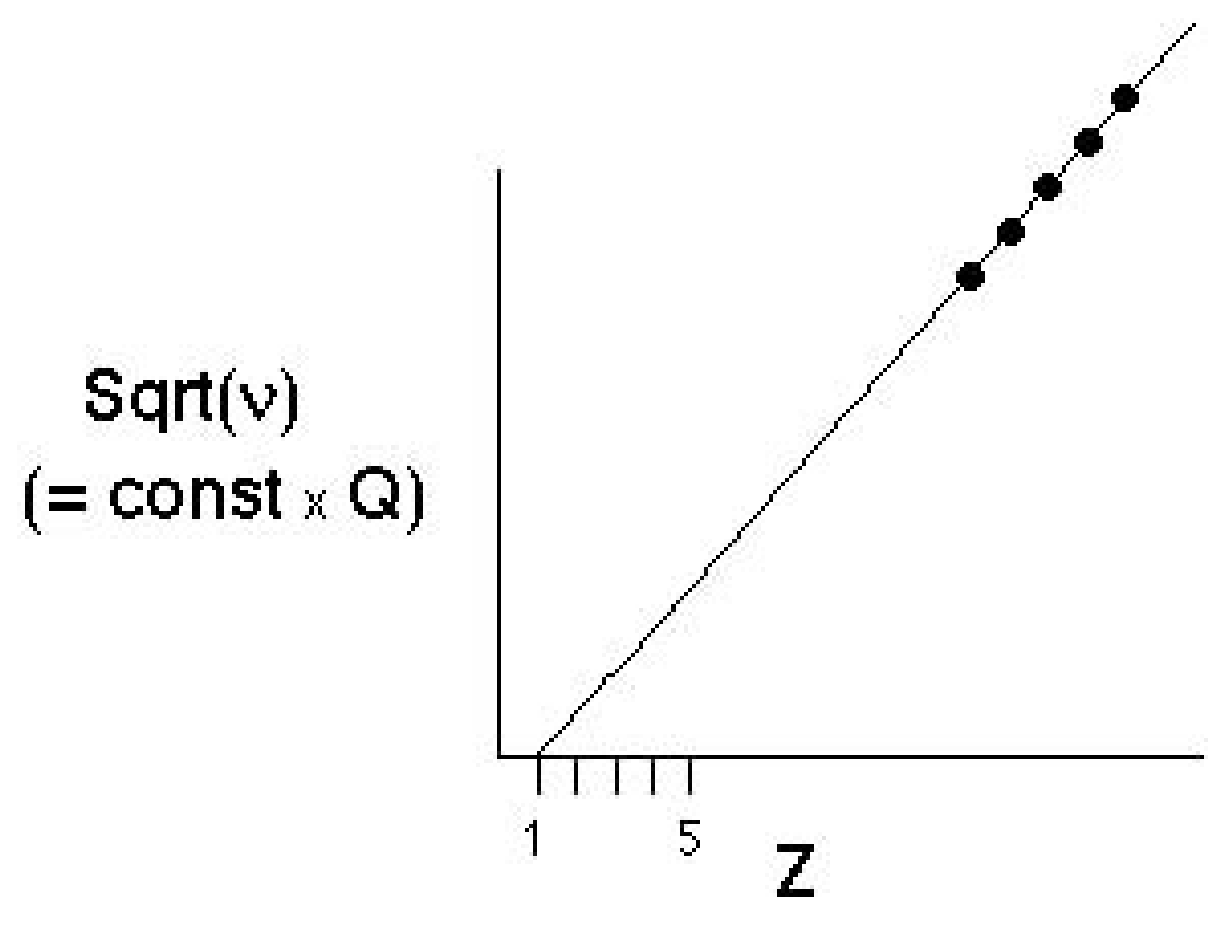
\includegraphics[clip,width=7cm]{BohrModel/4-5.ps}
\caption{X射线特征频率的平方根对原子序数Z作图满足线形关系}
\end{center}
\end{figure}

根据玻尔理论:

\begin{equation}
\nu  = cRZ^2 \left( {\frac{1}{{1^2 }} - \frac{1}{{2^2 }}} \right) \approx 0.246 \times 10^{16} Z^2 Hz
\end{equation}

公式中,$Z-1$表明跃迁电子受到$Z-1$个正电荷的有效电磁相互作用。

$K_\alpha $射线可解释为:
入射高能电子首先从原子内层$n=1$移去一个电子形成一个内层空穴,
然后外层$n=2$处电子跳到$n=1$填补空穴, 并发出射线。考虑屏蔽效应,
有效电荷应为$Z-1$ ($n=1$电子占满时, 有2个电子, 移去1个后, 还剩1个,
与原子核整体形成$Z-1$有效电荷)。同样,
我们可以解释L线系为:由外层电子跃迁至$L$($n=2$)层发出的光频率,
实验测得有效电荷为:$Z-7.5$。

\index{Characteristic radiation: 特征辐射}


\begin{figure}[h]
\begin{center}
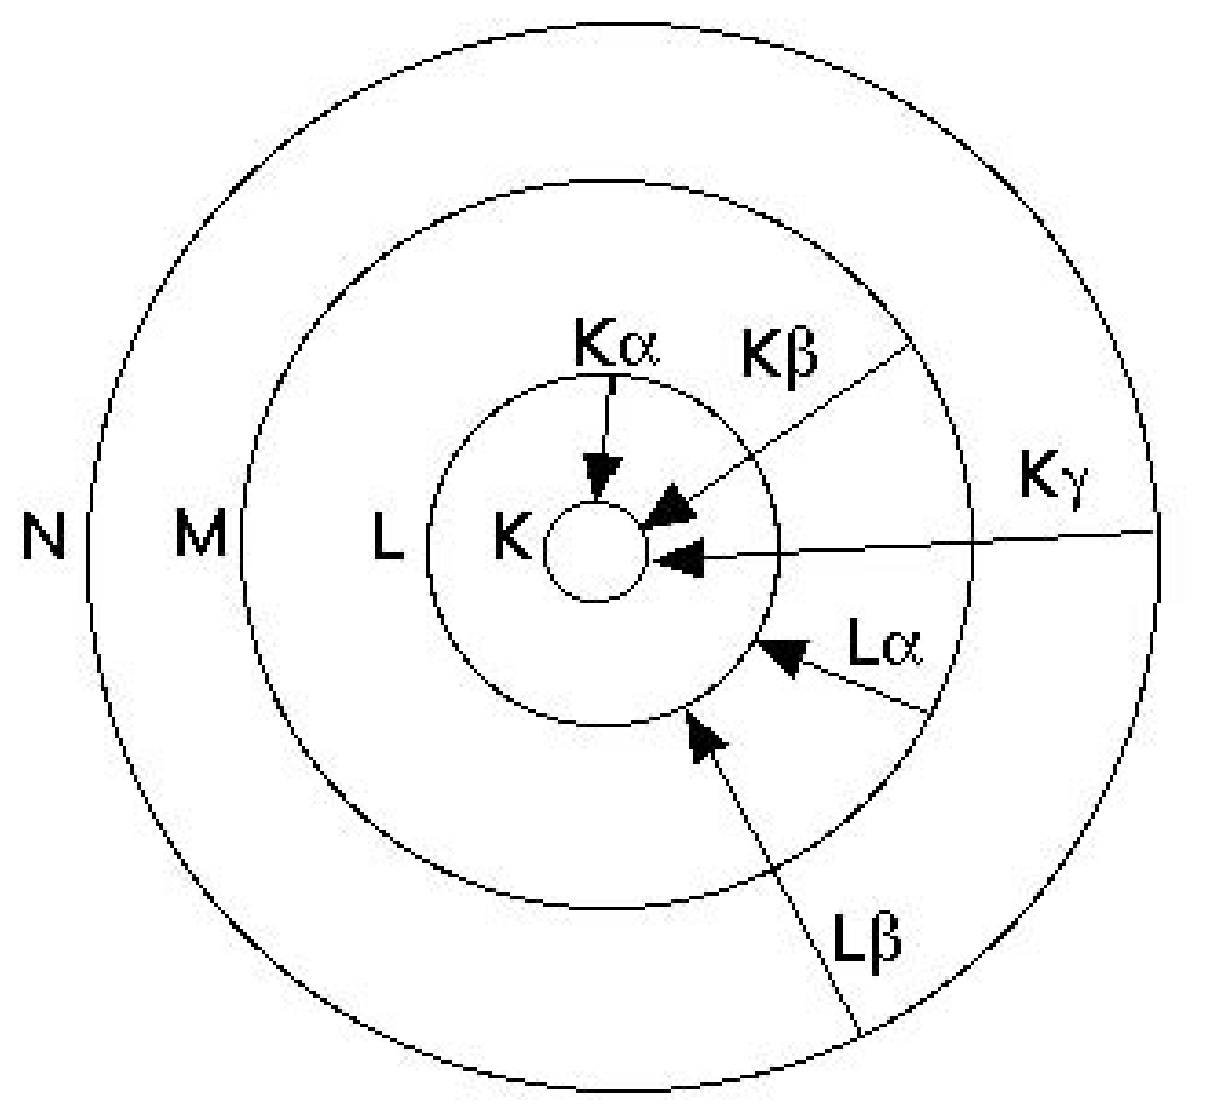
\includegraphics[clip,width=5cm]{BohrModel/4-6.ps}
\caption{X射线特征辐射:K线系(外层电子跃迁至n=1层)与L线系(外层电子跃迁至n=2层)}
\end{center}
\end{figure}



X射线的吸收限(吸收边缘):让X射线照射物体(吸收体),显然当入射X射线频率越高,吸收系数越小,
透射能力越强。但当入射X射线能量足以使一个$n=1$电子脱离原子时,则引起原子的共振吸收,对应为$K$吸收边缘。
同样也会存在$L$吸收边缘,$M$吸收边缘。如图:X射线由低频到高频分别是$L$吸收边缘和$K$吸收边缘。

\begin{figure}[h]
\begin{center}
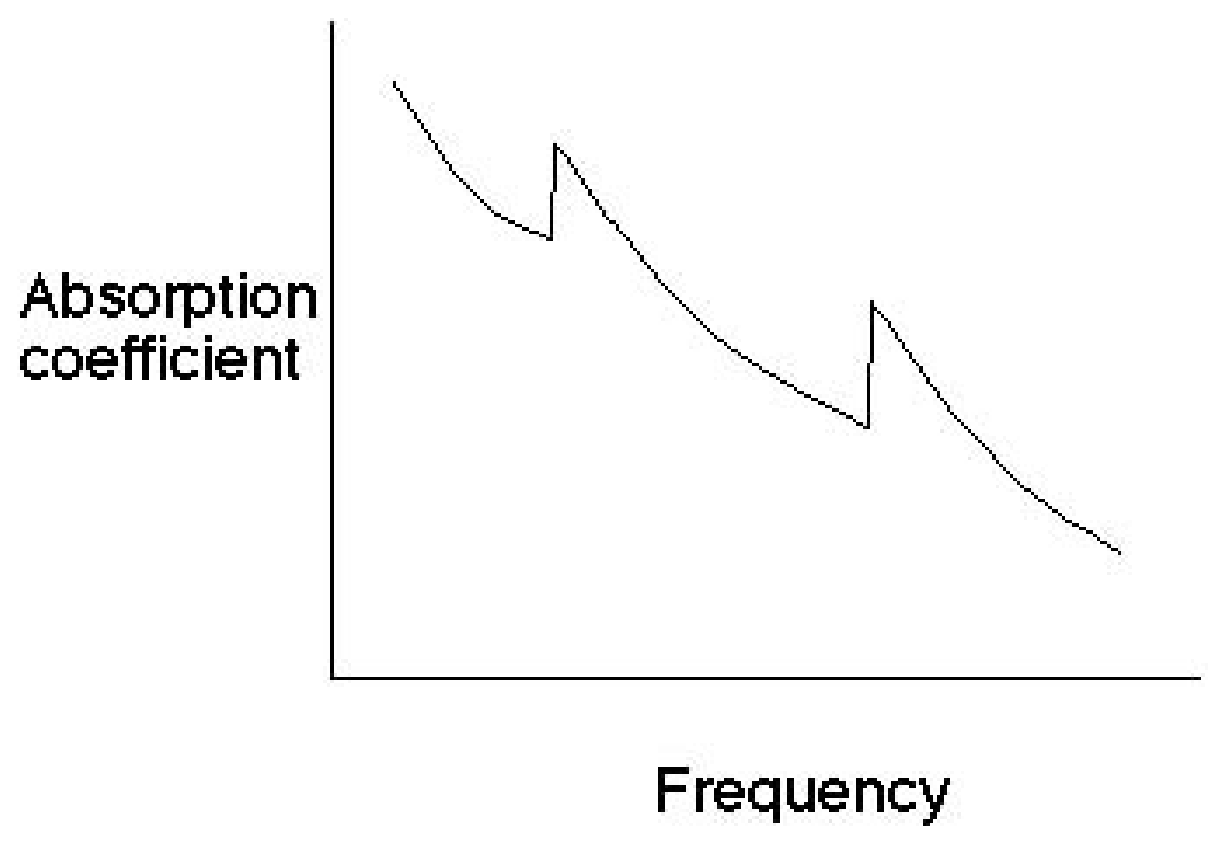
\includegraphics[clip,width=5cm]{BohrModel/4-8.ps}
\caption{X射线的吸收边缘}
\end{center}
\end{figure}

这是X射线成像技术的物理原理,如在医疗诊断中常用的CT(Computed
tomography)技术。


\subsubsection{俄歇效应}

\index{Auger effect: 俄歇效应}

\index{Auger electron: 俄歇电子}

原子壳层中产生空穴后, 产生X射线仅是释放能量的一种途径,
另一种途径是不释放X射线, 而把能量传递给另一层中的一个电子,
这个电子可以脱离原子, 称为俄歇电子,
这个过程称为俄歇电子发射。这个现象, 是法国科学家俄歇(P.
Auger)1923年发现的。一般说来, 轻元素, 发射俄歇电子的几率较大,
重元素发射X射线的几率较大。俄歇电子的动能完全决定于元素的本性,
因此对俄歇电子的测量也是进行材料分析的手段。


\begin{figure}[h]
\begin{center}
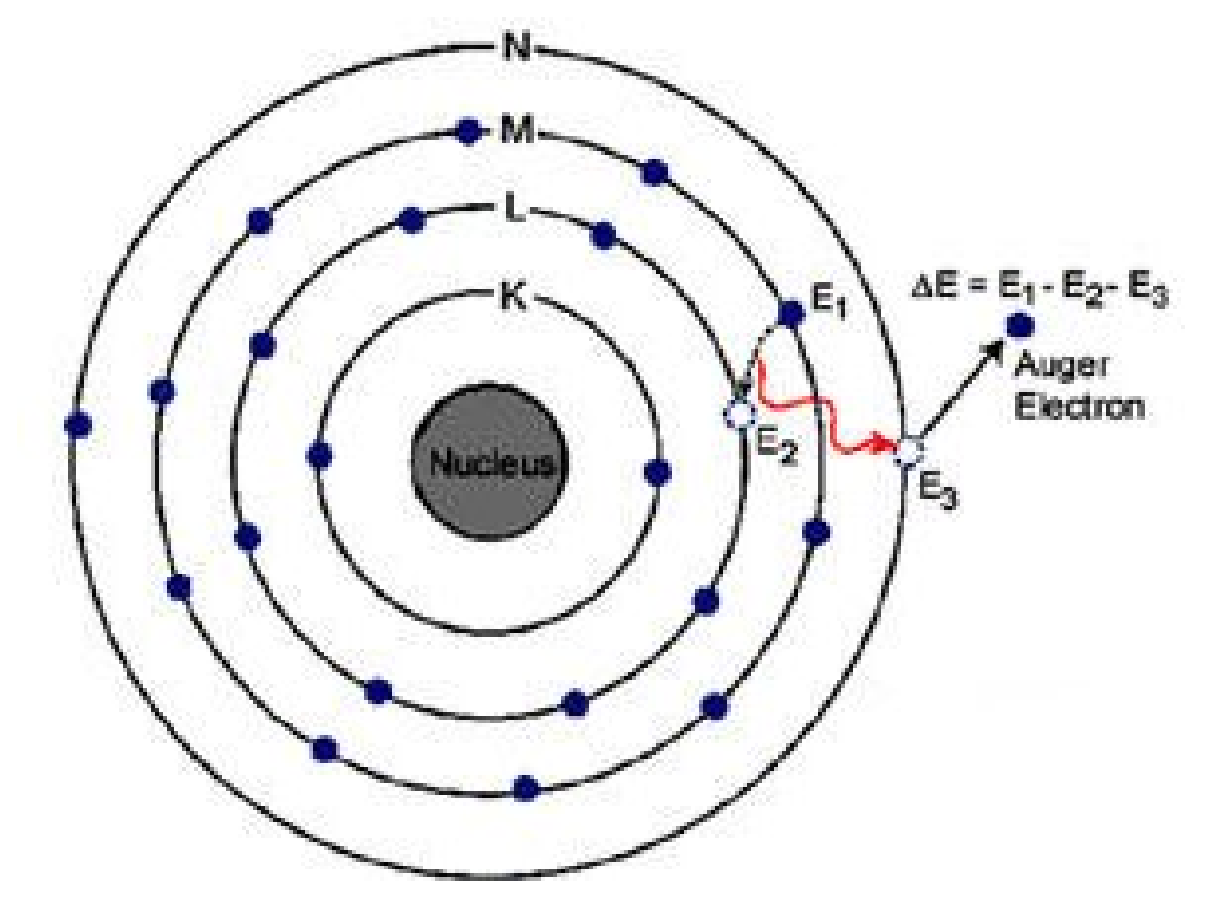
\includegraphics[clip,width=5cm]{BohrModel/auger-effect.ps}
\caption{俄歇电子发射}\label{auger electron}
\end{center}
\end{figure}


如图\ref{auger electron}, 较高能级电子湮灭空穴放出能量$E_1 - E_2$,
这个能量会激发某外层电子脱离原子而成为自由的,
在这个过程中要消耗能量$E_3$, 最终发射出的俄歇电子动能为: $E_k = E_1
- E_2 - E_3$



\subsection{玻尔-索末菲量子化条件}

\index{Bohr-Sommerfeld quantization condition:
玻尔-索末菲量子化条件}

玻尔角动量量子化条件仅适用于圆形轨道,
索末菲把玻尔量子化条件:$L = mvr = n\hbar $推广为:

\begin{equation}\label{Sommerfeld Condition}
    \oint {pdq = nh}
\end{equation}

其中$p$,$q$是一对共轭的正则坐标与正则动量,闭合回路积分代表对周期运动积分一个周期\footnote{
有兴趣的同学, 可自学: 褚圣麟编《原子物理学》, 第2.6节, pp48-55;
用这种方法可推出考虑相对论效应后的光谱项是:

\begin{equation*}
T(n,n_{\phi})=\frac{RZ^2}{n^2}+\frac{Rz^4\alpha^2}{n^4}\left(
\frac{n}{n_{\phi}}-\frac{3}{4}\right)+...,
\end{equation*}

即褚圣麟书中pp55中第(16)式。

},但有时这样作会求出很荒谬的结果。

\index{Canonical coordinate: 正则坐标}

\index{Canonical momentum: 正则动量}


\subsubsection*{卢瑟福对玻尔理论的批评}

玻尔理论在卢瑟福模型基础上, 用经典力学处理电子围绕原子核的运动,
引入了定态假设、角动量量子化条件。但这些多少带有人为的性质,
而不是严密的理论体系。卢瑟福在1913年3月20日给玻尔的信中写道\footnote{《尼耳斯·玻尔集》第二卷,
pp112}:


\begin{quote}
    你的关于氢光谱的起源方式的想法是很巧妙的, 而且看来也是很好用的;
    但是,
    普朗克概念和旧力学的混合却使人很难对什么是它的基础形成一个物理概念。在我看来,
    你的假说中有一个严重的困难,
    这个困难我毫不怀疑地认为你也充分意识到了, 那就是,
    当电子从一个定态过渡到另一个定态时,
    它怎么决定将以什么频率来振动呢? 在我看来,
    你必须假设电子事先就知道它将在什么地方停下来。
\end{quote}

\index{Old quantum theory: 旧量子论}


我们现在知道玻尔理论不是真正意义上的量子力学,
因此也称作``旧量子论''或``半经典的量子力学''。
玻尔等也尝试推广玻尔模型以适用于更复杂的一些原子(如氦),
但都失败了, 此外玻尔模型只能解释氢光谱线的位置,
而不能解释谱线的强度。因此为玻尔模型提供一个更坚实的理论基础,
发展出能够一般性地解决原子光谱现象的新力学就成为自然的任务。

\subsection*{物理常数}

\begin{itemize}
  \item 万有引力常数: $G = 6.67 \times 10^{ - 11} m^3 \cdot kg^{-1} \cdot s^{-2} $

\item 精细结构常数: $\frac{e^2}{4 \pi \epsilon_0 \hbar c} = \alpha \approx \frac{1}{137}$

  \item 氢原子的电离能: $E_{\infty} = 13.6eV$
  \item 氢原子的第一玻尔半径: $a_0 = r_1 \approx 0.053 nm$, $r_n = n^2 a_0$

  \item 氢原子的第一玻尔速度: $v_1 = \alpha c$, $v_n = \frac{\alpha c}{n}$
\end{itemize}


\subsection*{练习}


\begin{enumerate}
\item 假设恒星可按绝对黑体处理, 估算恒星表面温度为多少时, 恒星发出的辐射可使其周围的氢电离。

解: 氢原子的电离能是$13.6eV$, 相当于: $13.6 \times 1.602 \times
10^{-19} = 2.18 \times 10^{-18} J$, 能使氢原子电离的光子的波长是,

\begin{equation*}
\lambda = \frac{hc}{\varepsilon}=\frac{6.626 \times 10^{-34} \times
3.0 \times 10^8}{2.18 \times 10^{-18}} = 9.1 \times 10^{-8}m
\end{equation*}

根据维恩位移定律, $\lambda_{max} T = 2.898 \times 10^{-3} m \cdot
K$,

\begin{equation*}
T = \frac{2.898 \times 10^{-3}}{9.1 \times 10^{-8}}=3.0\times 10^4 K
\end{equation*}

即需要大约三万K使恒星附近的氢原子电离.
或者说当整个宇宙的背景温度是三万K时, 自由的氢原子是不可能存在的,
只有质子和电子.

作为比较, 我们知道像太阳那样的恒星, 其表面温度是大约5780K.
对应$\lambda_{max}$是:

\begin{equation*}
\lambda_{max} = \frac{2.898 \times 10^{-3}}{5780} = 500 nm
\end{equation*}

能量是:

\begin{equation*}
\varepsilon =h \nu = \frac{hc}{\lambda}= \frac{6.626 \times 10^{-34}
\times 3.0 \times 10^8}{5.0 \times 10^{-7}}= 4.0 \times 10^{-19} J
\end{equation*}

相当于: $\frac{4.0 \times 10^{-19}}{1.602 \times 10^{-19}}=2.5
\text{eV}$.

如果是一颗红星, 取$\lambda_{max}=650 nm =6.5 \times 10^{-7}m$,
红星表面的温度是:

\begin{equation*}
T = \frac{2.898 \times 10^{-3}}{6.5 \times 10^{-7}}=4400K
\end{equation*}

即红星表面温度仍高达4400K.

  \item 电子偶素是由一个正电子和一个电子所组成的一种束缚系统,试求:
(1)基态时两电子之间的距离;(2)基态电子的电离能和由基态到第一激发态的激发能;
(3)由第一激发态退激到基态所放光子的波长。

\item 电子和质子间的引力是$\frac{Gm_pm_e}{r^2}$, 假设只考虑引力而忽略电磁相互作用. 按照玻尔理论估算氢原子的第一玻尔半径(请把最终结果用光年表示).

\item $He^+$离子的电离能是多少? (答: $13.6 eV \times 4 = 54.4 eV$)

\item 利用“玻尔-索末菲量子化条件”求一维谐振子的能量,并说明其是量子化的。

\end{enumerate}


\subsection*{阅读}

关于里德堡原子和量子信息(量子计算),请阅读:

Quantum information with Rydberg atoms, Rev. Mod. Phys. 82,
2313–2363 (2010).

\url{http://rmp.aps.org/abstract/RMP/v82/i3/p2313_1}

\section{粒子的波动性}

\begin{quotation}
“粒子是一种观念形态的概念,它产生于我们为了表示事物在给定时刻处于空间某点的定位的思想。” \qquad 德布罗意
\end{quotation}

\subsection{物质波的概念}

\begin{figure}[h]
\begin{center}
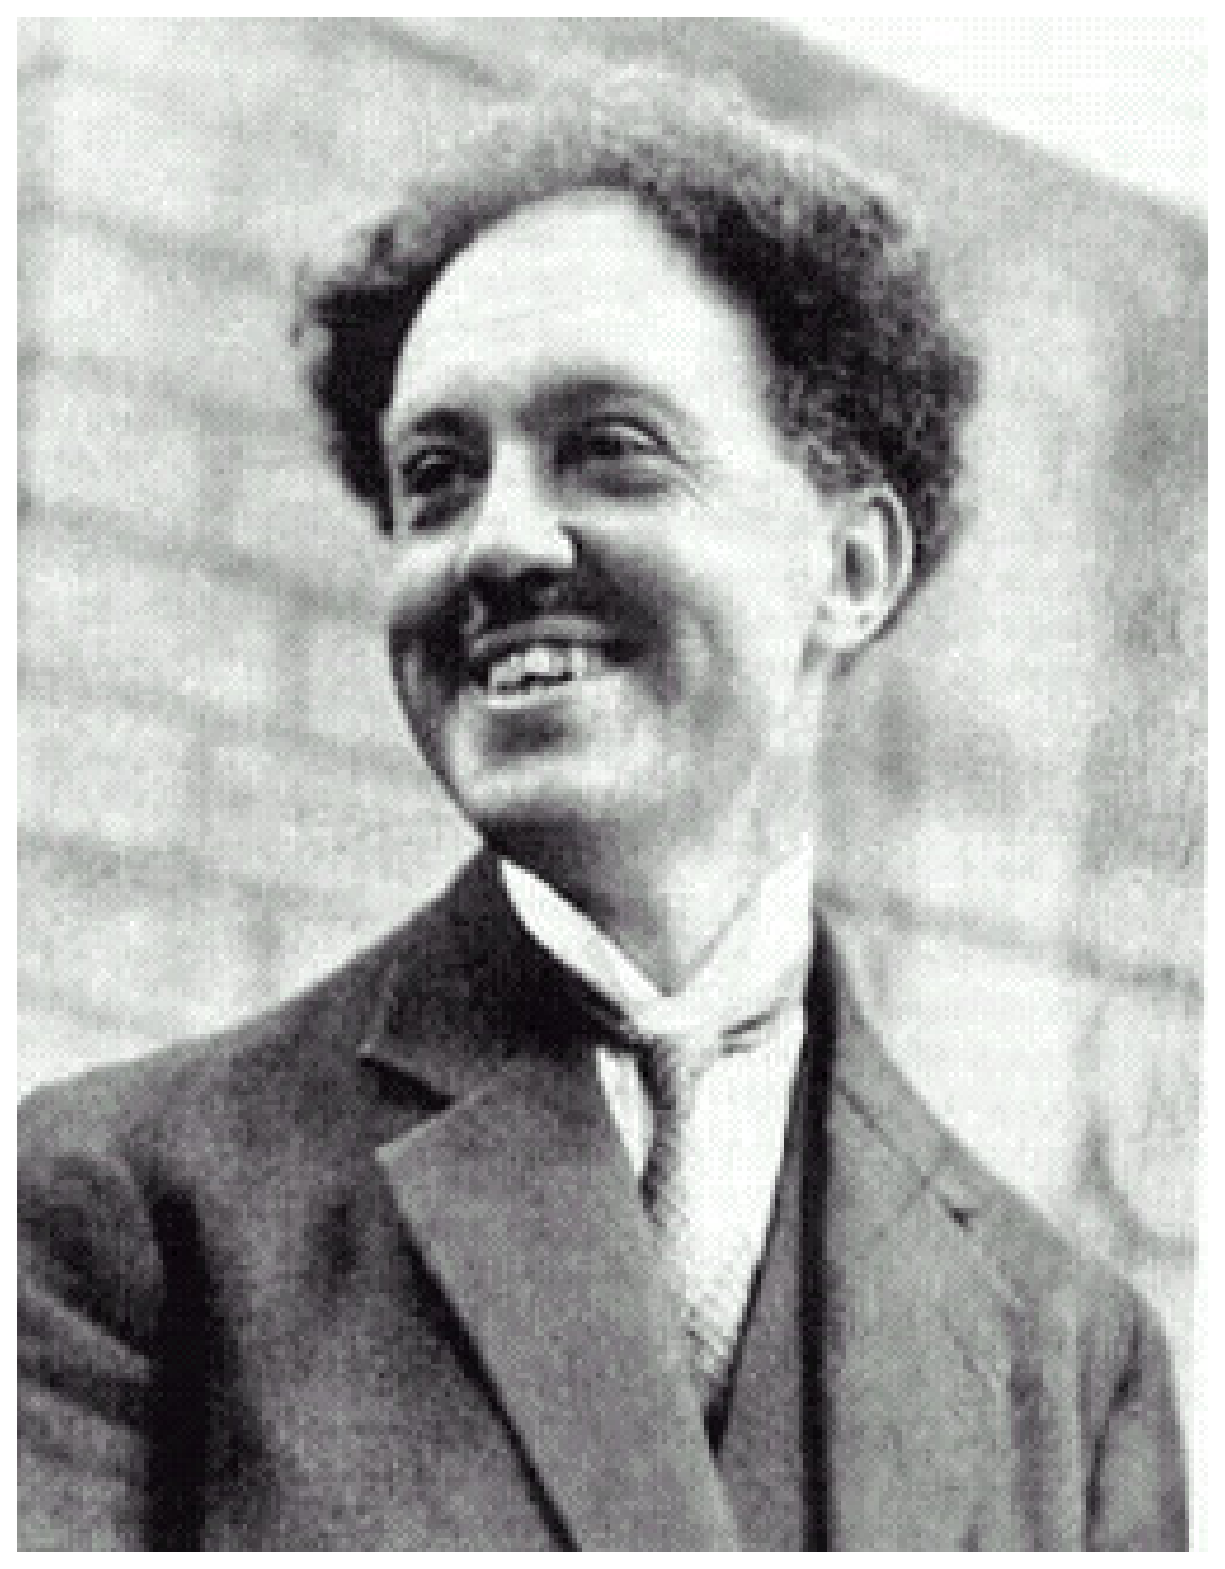
\includegraphics[clip,width=6cm]{Duality/debroglie.ps}
\caption{德布罗意}
\end{center}
\end{figure}

\subsubsection*{宏观物理学与微观物理学的对立}

玻尔的原子理论向我们揭示,微观尺度的物理学规律与宏观尺度的经典物理学规律是不同的。
光波在宏观尺度是经典的波动(连续形式的运动),而在微观尺度则体现为波粒二象性(wave-particle
duality), 既有波动性又有粒子性。

1923年,德布罗意(de
Broglie)提出:对物质粒子而言在微观尺度同样应具有``波粒二象性''的假设,
即在微观尺度,电子会体现出波动性,
有干涉、衍射现象,可以用波动方程表示微观粒子的运动。

\index{Quantization of angular momentum: 角动量量子化}

德布罗意受玻尔理论启发,``角动量量子化''为原子的定态运动引入了整数$n$,而在经典物理学中,``驻波''也对应整数$n$。
玻尔理论中角动量量子化:

$L = mvr = n\hbar $ $\Rightarrow$ $pr = \frac{{nh}}{{2\pi }}$
$\Rightarrow$ $2\pi r = \frac{{nh}}{p}$

\begin{figure}[h]
\begin{center}
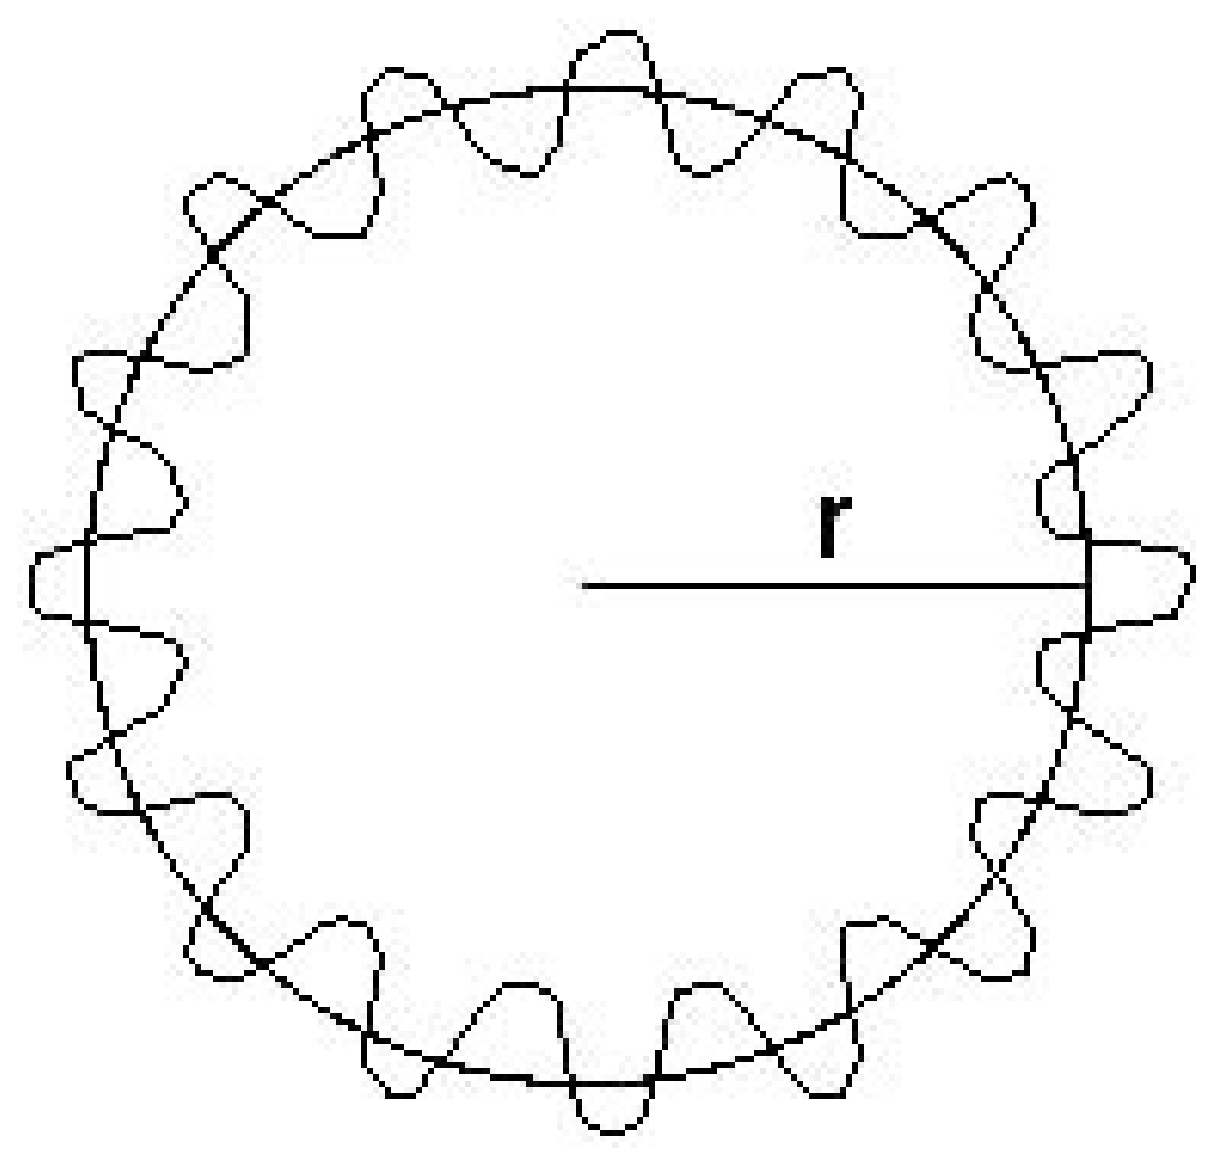
\includegraphics[clip,width=6cm]{Duality/5-1.ps}
\caption{电子在半径为r圆轨道上的驻波}
\end{center}
\end{figure}

\index{Standing wave: 驻波}

如果把玻尔理论中的定态对应为电子在圆轨道上的驻波,则:$2\pi r = n\lambda  = n\frac{h}{p}$
(即:电子围绕原子核运动一周,相位正好变化 的整数倍,同位相波动相长。)

得到德布洛意关系式:

\begin{equation}\label{5-1}
\lambda  = \frac{h}{p}
\end{equation}


这样就把粒子的特征:动量($p$)与波动的特征:波长($\lambda$ )联系了起来。

利用普朗克量子化条件也可以把粒子的能量与波动的频率联系起来:$\nu  =
\frac{\varepsilon }{h}$, 形式上与表示光的波粒二象性所用方程一样,
$\lambda ,\nu $ 分别是物质波的波长和频率。
(由于光子静质量为$0$,也可把物质波看作是``波粒二象性''由质量为$0$情形向质量不为$0$情形的推广)

这样微观粒子的运动状态可用波动方程表示,如对自由粒子,具有确定的能量$E$和动量$p$,所以对应描写波动的函数为一个平面波(plane
wave): $\psi  = A\cos \left[ {k \cdot r - \omega t} \right],k =
\frac{{2\pi }}{\lambda }\hat n,\omega  = 2\pi \nu $ ,这里$\hat
n$是波动传播方向(粒子运动方向)的单位矢量。

这个波函数(wave function)也可写为复数形式:

\begin{equation}
\psi  = Ae^{i(k \cdot r - \omega t)} = Ae^{\frac{i}{\hbar }(p \cdot
r - Et)}
\end{equation}

这种波称为德布罗意波或物质波(matter wave)。

\textbf{例1:相对论情形和非相对论情形下的德布罗意关系式:}

对于非相对论情形,$\varepsilon _k  = \frac{{p^2 }}{{2m_0 }}$,$p = \sqrt {2m_0 \varepsilon _k } $

相对论情形:$E^2  = p^2 c^2  + m_0 ^2 c^4 $,


$p = \frac{1}{c}\sqrt {E^2  - m_0 ^2 c^4 }  = \frac{1}{c}\sqrt
{\left( {m_0 c^2  + \varepsilon _k } \right)^2  - m_0 ^2 c^4 } $

$ = \frac{1}{c}\sqrt {\varepsilon _k ^2  + 2m_0 c^2 \varepsilon _k }
 = \sqrt {2m_0 \varepsilon _k  + \left( {{\textstyle{{\varepsilon
_k } \over c}}} \right)^2 } $

所以当$\varepsilon _k  \ll c$时,即得到非相对论情形下的公式。

$\nu  = \frac{E}{h} = \frac{{\sqrt {p^2 c^2  + m_0 ^2 c^4 } }}{h} =
\frac{{m_0 c^2 }}{h}\left( {1 + \frac{1}{2}\left( {\frac{{p^2 c^2
}}{{m_0 ^2 c^4 }}} \right) + ...} \right) $

$ = \frac{{m_0 c^2 }}{h}\left( {1 + \frac{{p^2 }}{{2m_0 ^2 c^2 }} +
...} \right) = \frac{1}{h}\left( {m_0 c^2  + \frac{{p^2 }}{{2m_0 }}
+ ...} \right)$

由于能量只有相对变化$\Delta E$才有意义(即能量的绝对值在物理上是没有意义的,它依赖于``零能量值''的选取),$h\nu  = \Delta E = E_2  - E_1 $ ,可将常数项$m_0 c^2 $抵消,此时相对论形式的关系退化为非相对论情形:$\nu  = \frac{{\varepsilon _k }}{h}$,$\varepsilon _k $就是非相对论粒子的动能。

德布罗意频率本身不是一个可观测量,只有德布罗意波长具有物理意义。

\textbf{例2:为什么物质的波动性在宏观尺度不显现}

由$\lambda  = \frac{h}{p}$,原因是普朗克常数太小($h = 6.6 \times 10^{ - 34} J \cdot s$),而宏观尺度的运动动量太大。如考虑一个50kg的人运动速度是0.5m/s,则可计算出对应物质波波长为:
$\lambda  = \frac{h}{p} = \frac{{6.6 \times 10^{ - 34} J \cdot s}}{{\left( {50} \right)\left( {0.5} \right)\left( {kg \cdot m/s} \right)}} = 2.6 \times 10^{ - 35} m$。
显然太小,难以引起可以观察的物理效应。

$p = \sqrt {2mE} $, 要减小宏观尺度运动的动量, 必须减小动能$E$,
但从物理上考虑$E$不可能减小到比热运动能量$k_B T$更小,
所以必须减小质量。质量的减小对应于尺度的减小。只有把物体尺度减小到微观尺度,
才可能出现较大的物质波波长 $\lambda$,从而引起可以观察到的物理效应。


\subsection{戴维孙-革末实验}

考虑电子被$V$伏特电场加速, $\lambda  = \frac{h}{p} =
\frac{h}{{\sqrt {2m_e E} }} = \frac{h}{{\sqrt {2m_e eV} }} \approx
\frac{{12.27}}{{\sqrt V }} {\AA}$.

当$V=150$伏时,$\lambda  = 1 {\AA}$。
如果用间距为1埃数量级的光栅,则应观察到入射电子的干涉条纹,人工加工这么小的尺度显然是困难的,
但自然界中单晶原子间距恰好大约是1埃,所以单晶可用作验证物质波假说的光栅。

\begin{figure}[ht]
\begin{center}
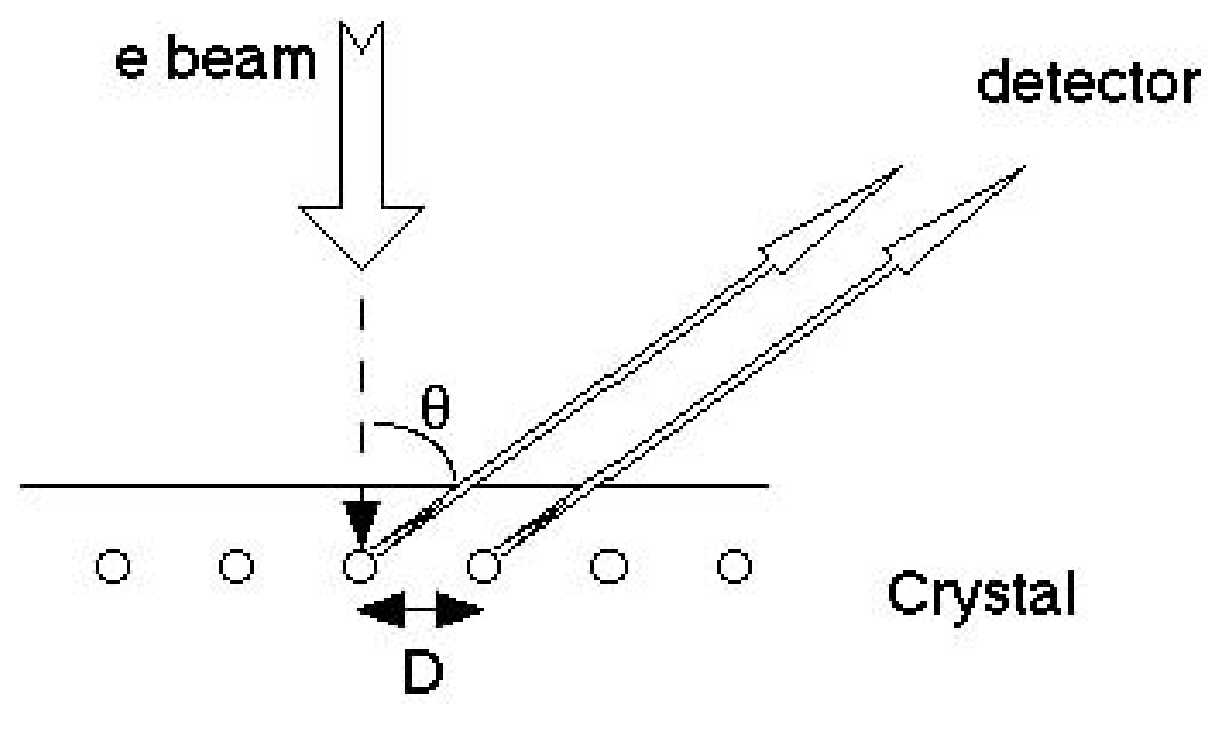
\includegraphics[clip,width=7cm]{Duality/5-2.ps}
\caption{电子被单晶衍射}
\end{center}
\end{figure}


对某晶面干涉相长条件:

\begin{center}
\begin{equation}
\label{bragg condition}
    D\sin \theta  = n\lambda
\end{equation}
\end{center}

$D$为晶面上相临原子间距,也叫布拉格条件(Bragg condition), 注意:
因角度$\theta$的选取不同, 布拉格公式的具体形式可能会有不同。

\index{Bragg's formula: 布拉格公式}

\index{Davisson–Germer experiment: 戴维孙-革末实验}

1925年,戴维孙(Davisson)和革末(Germer)在做电子在镍(Ni)单晶上散射实验时,第一次观察到电子在晶体中的衍射现象。
散射电子强度在特定方向$\theta$出现极大值。
实验证明微观粒子确实具有波动性质,所以和光一样,物质粒子也具有``波粒二象性''。

\index{Wave-particle duality: 波粒二象性}


\begin{figure}[ht]
\centering
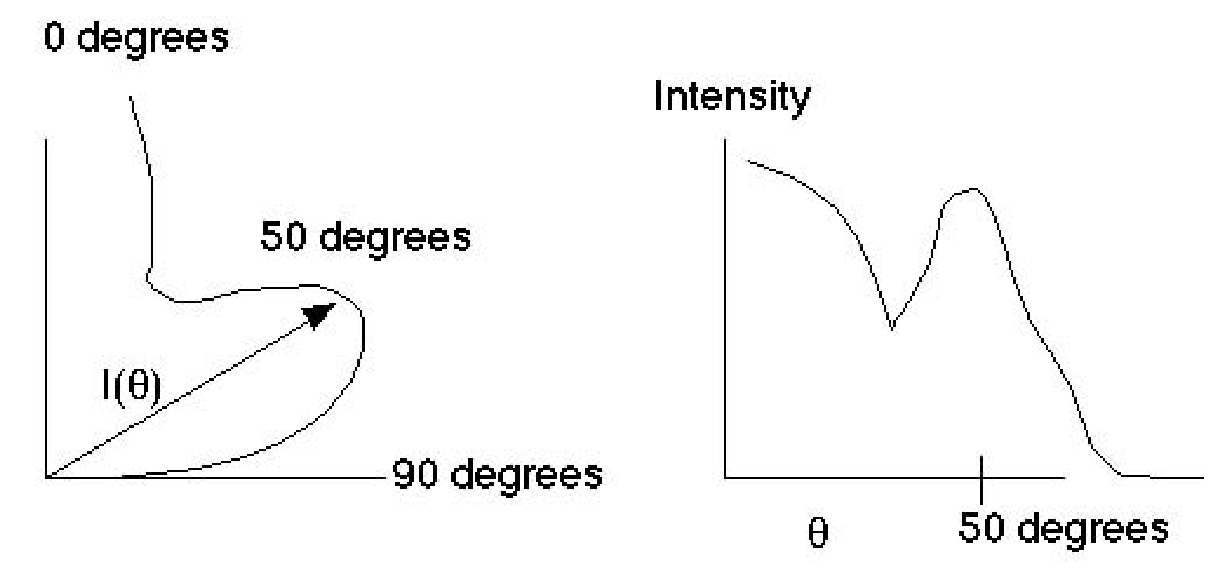
\includegraphics[width=8cm]{Duality/5-3.ps}
\caption{电子在单晶中的衍射图样}
\end{figure}



\subsection{电子的双缝干涉实验}

为说明电子的波粒二象性,我们做``电子双缝干涉''(double-slit
experiment)的理想实验\footnote{这个理想实验在费曼物理学讲义中有详细讨论,
最近确实有实验物理学家在实验室里实现了``电子的双缝干涉'',请参考:

\url{http://physicsworld.com/cws/article/print/2002/sep/01/the-double-slit-experiment}

}。

\index{Double-slit experiment: 双缝实验}

(1)一束电子通过双缝:

\begin{figure}[ht]
\begin{center}
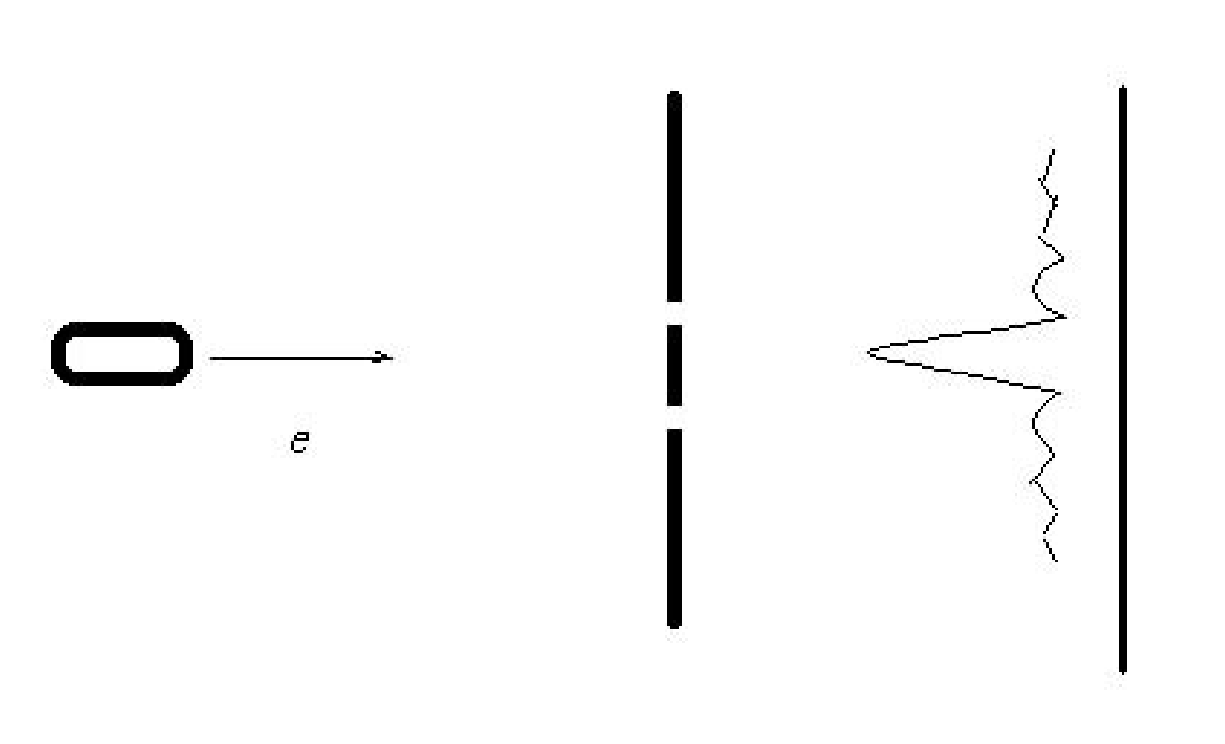
\includegraphics[clip,width=6cm]{Duality/5-4.ps}
\caption{一束电子通过双缝}\label{Duality/5-4-ps}
\end{center}
\end{figure}

在屏上可观察到干涉条纹,说明电子确实有波的性质。(如图\ref{5-4-ps})

问题:波动性质(干涉效应的出现)是电子的集体行为(不同电子间干涉)?
还是电子本身的性质(每个电子自己和自己发生干涉效应)?

(2)单电子干涉

\begin{figure}[ht]
\begin{center}
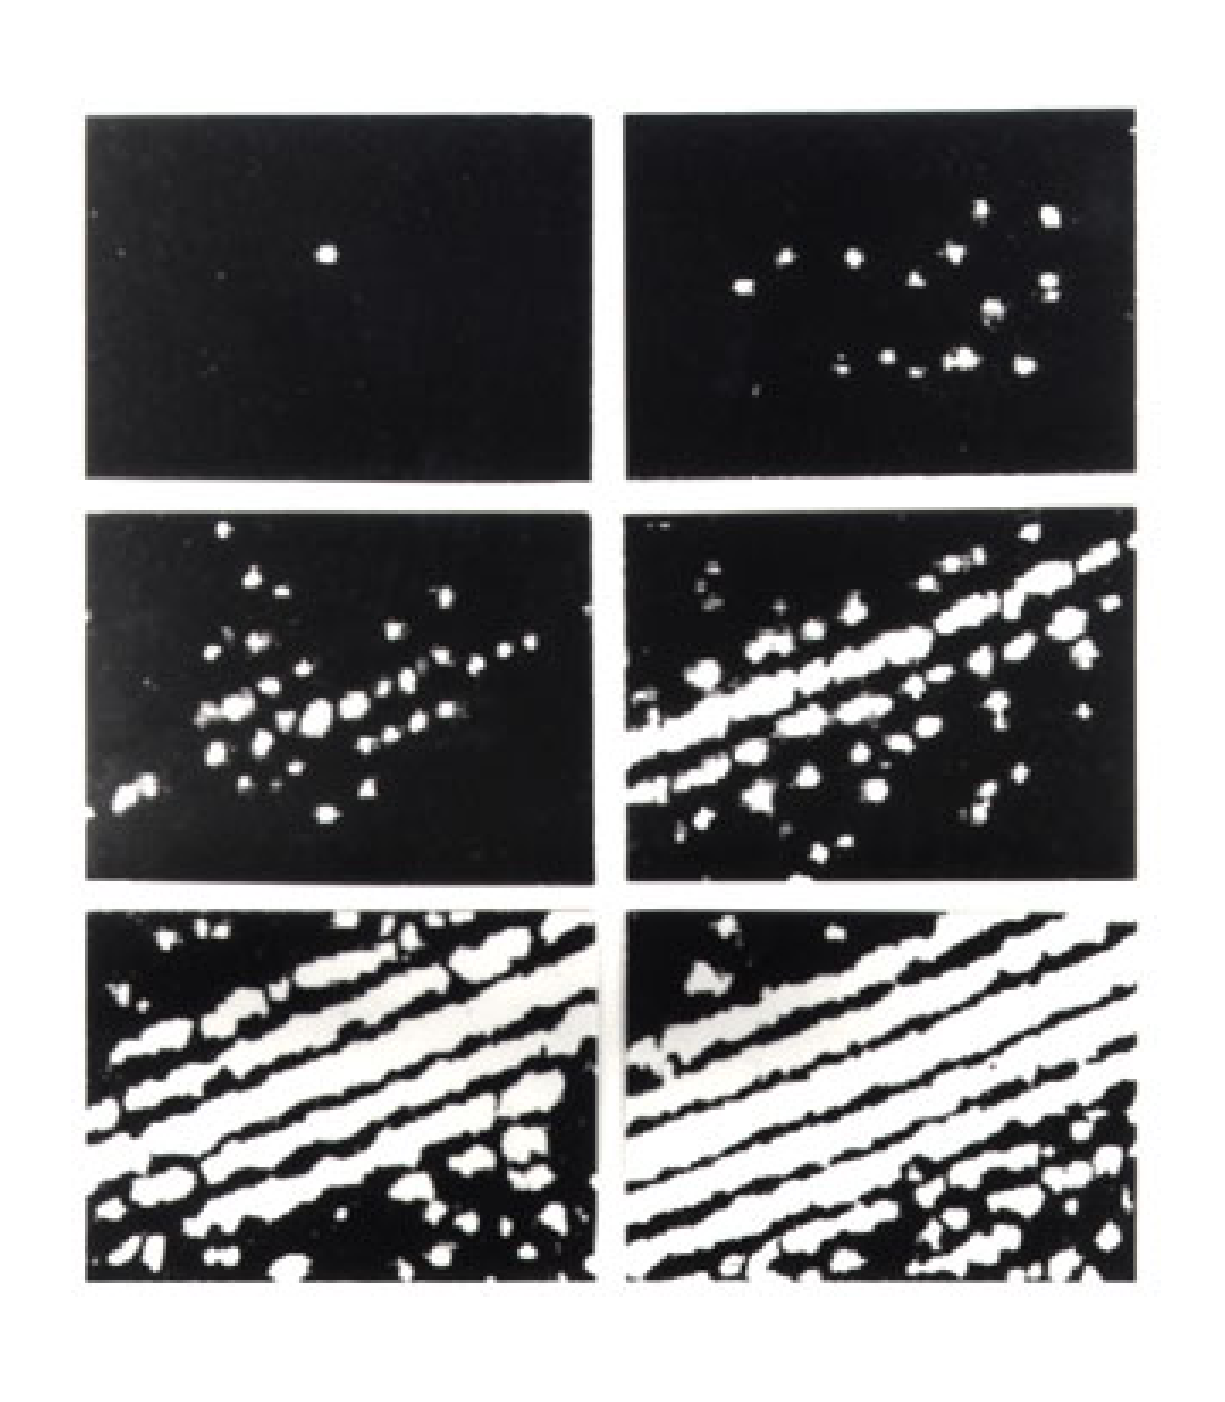
\includegraphics[clip,width=6cm]{Duality/double-slit.ps}
\caption{实验观察到的``单电子干涉''}\label{5-4-ps}
\end{center}
\end{figure}


为解决实验(1)所提出的问题,我们可以做单电子干涉实验,即让电子一个一个地穿过双缝,看会发生什么。

实验结果显示:

电子只在屏上一点被探测到,说明电子是穿过双缝之一,并没有``一分为二'',分别穿过两个缝(体现为粒子性)。
但电子在屏上出现的具体位置是没有规律的,若长时间观察,电子一个一个累计的效果是再次出现干涉条纹(体现为波动性)。
不同电子穿过双缝分别都是独立事件,每个电子在屏上出现的几率分布$P(x)$应是相同的。
单电子也体现出波动性,即波动性是微观粒子的本质属性,
或``波粒二象性''是微观粒子的本质属性。

(3)挡住一条缝

\begin{figure}[ht]
\begin{center}
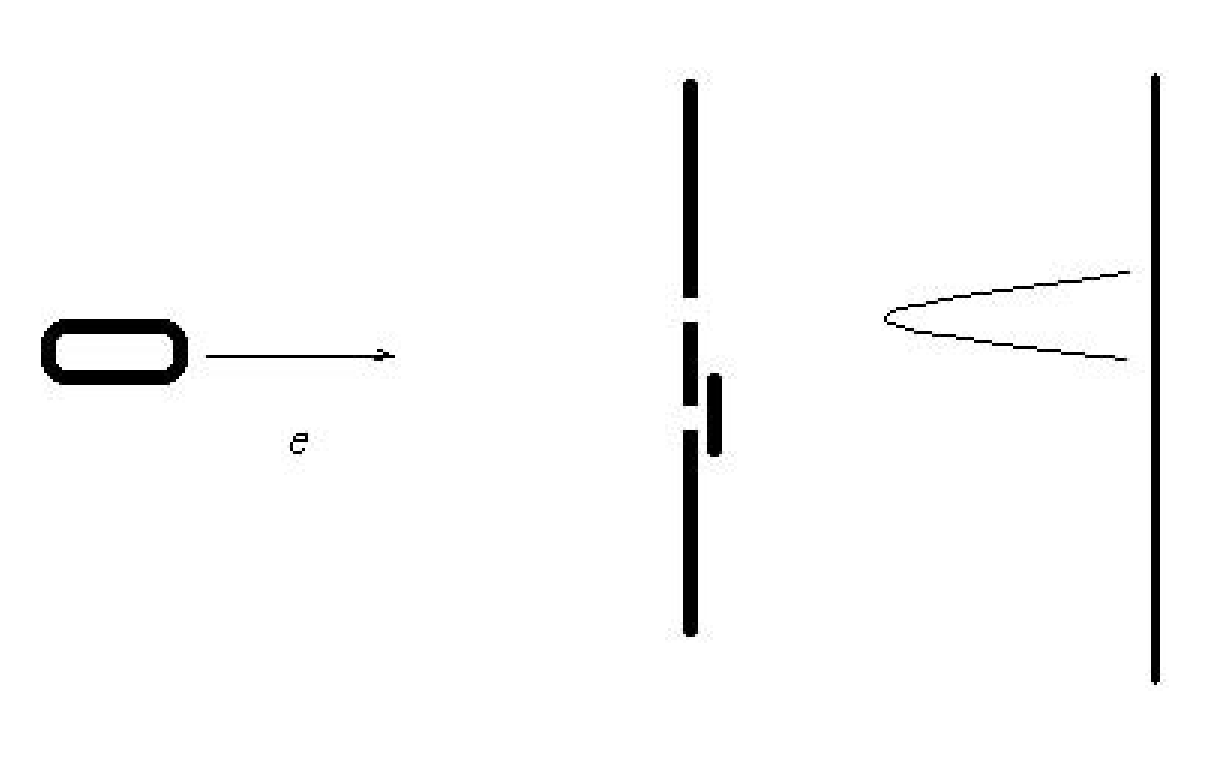
\includegraphics[clip,width=6cm]{Duality/5-5.ps}
\caption{挡住一条缝,干涉条纹消失}\label{5-5-ps}
\end{center}
\end{figure}

干涉条纹消失,电子集中在未遮挡缝延长方向上,表现为粒子性,如图\ref{5-5-ps}。(为叙述方便,我们先不考虑单缝衍射效应)

(4)控制开关,人为地遮挡两个缝中的任何一个

\begin{figure}[ht]
\begin{center}
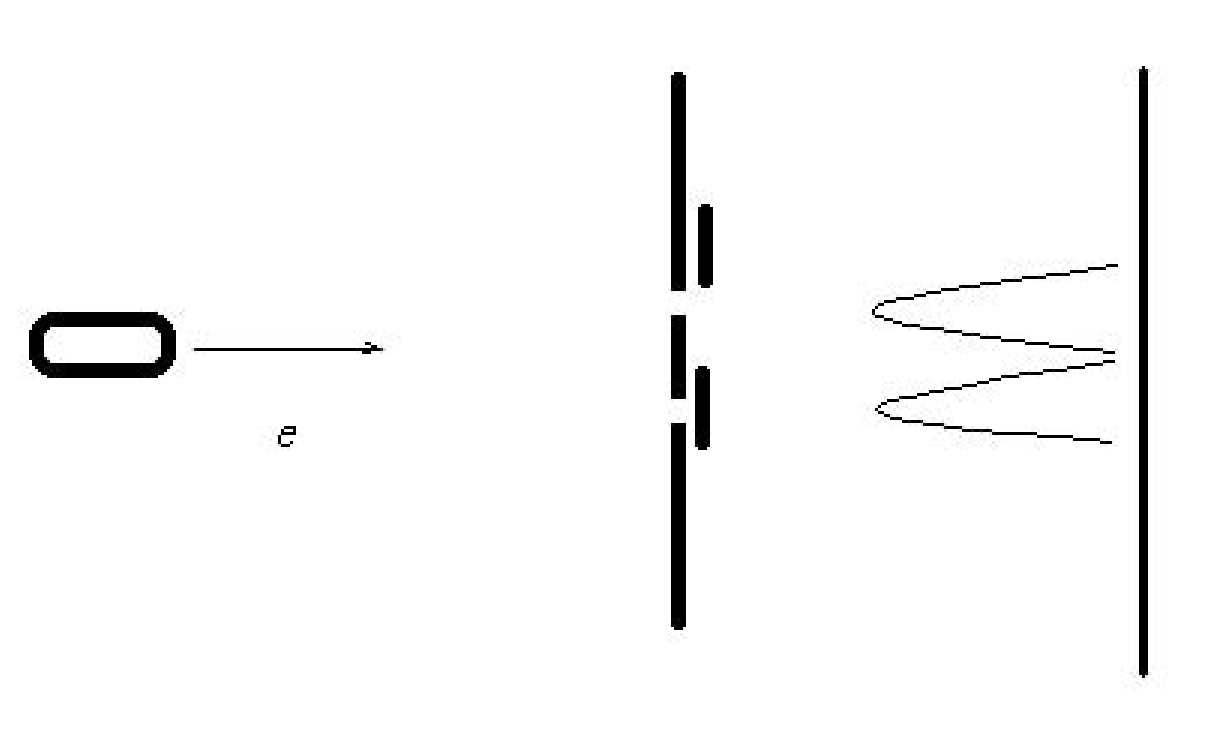
\includegraphics[clip,width=6cm]{Duality/5-6.ps}
\caption{人为地遮挡两个缝中的任何一个}\label{5-6-ps}
\end{center}
\end{figure}

我们任意地遮挡住两个缝中任何一个,遮挡顺序是无序的,但必须确定,即是人为可以控制的。
这时,干涉条纹消失,电子穿过双缝积累效果是电子集中在双缝方向分布,出现两个峰,如图\ref{5-6-ps},体现为粒子性。

(5)在``双缝''处分别安装测量装置,使之可以测量电子究竟是从哪个缝穿过的。

这种可以测量电子位置的装置是一种``理想装置'',它的作用就是获取电子的位置信息,
至于它是如何实现的\footnote{我们可以使用光子来探测电子的位置,即在双缝两边各放一光源($P_1$, $P_2$)和一光探测器($D_1$, $D_2$)。
光源发出的光子打在经过狭缝的电子上,被散射出来由探测器记录,并给出信号。参考杨福家《原子物理学》第97页。},在这里我们并不关心。

实验结果是:如每个电子穿过哪条缝都被成功观测到,则干涉条纹消失。
电子穿过双缝积累效果是电子集中在双缝方向分布,出现两个峰。(体现为:粒子性)

实验(5)与实验(4)本质上是相同的,即系统是``单缝''而不是``双缝'',所以不会发生干涉。
一旦我们可以确认电子是由哪条单缝穿过的,另一条单缝对电子来说就是``不存在''的,即相当于另一条单缝被遮挡。

\subsection{海森堡不确定关系}

\begin{figure}[h]
\begin{center}
\includegraphics[clip,width=6cm]{Duality/bohr-hei.ps}
\caption{海森堡在哥本哈根与玻尔工作期间提出了不确定原理}
\end{center}
\end{figure}


\begin{figure}[ht]
\begin{center}
\includegraphics[clip,width=5cm]{Duality/5-7.ps}
\caption{测不准关系示意}\label{5-7-ps}
\end{center}
\end{figure}


不确定关系(uncertainty relation,
也叫测不准关系)是海森堡(Heisenberg)1927年首先提出的:

\index{Uncertainty principle: 不确定原理}

\begin{center}
\begin{eqnarray}
% \nonumber to remove numbering (before each equation)
  \Delta p_x \Delta x \ge h\\
  \Delta E\Delta t \ge h
\end{eqnarray}
\end{center}

不确定关系还有多种其他表示形式,这是其中最常用的两个。
不确定关系表明,微观粒子在客观上不能同时具有确定的坐标及相应确定的动量。

如图\ref{5-7-ps},考虑电子双缝干涉,两缝间距为$l$;
为测量电子是从哪个缝中射出,光源P发出的测量光子必须具备至少$l$的分辨本领,即:$\lambda
\le l$。 则测量光子至少具备动量:$p \ge \frac{h}{l}$。
测量光子转移给电子的动量为:$\Delta p \ge \frac{h}{l}$,
假设测量光子动量全部转移。所以光子对电子测量结果:$\Delta x =
l,\Delta p \ge \frac{h}{l}$, 即:$\Delta p_x \Delta x \ge
h$,这是不确定关系的粗略推导,严格证明我们将在后续的章节中给出。

\textbf{例3:谱线的自然宽度}

\begin{figure}[ht]
\begin{center}
\includegraphics[clip,width=5cm]{Duality/5-8.ps}
\caption{谱线的自然宽度}\label{5-8-ps}
\end{center}
\end{figure}

\index{Natural width of spectral line: 谱线的自然宽度}

\index{Energy-Time Uncertainty Relation: 能量-时间不确定关系}

假设电子在激发态(能量较高的能级)具有一定寿命$\Delta
t$,即电子被激发到激发态后,再过$\Delta t$
跃迁回基态。这样激发态能量对应有一个不确定值$\Delta E \sim
\frac{h}{{\Delta t}}$。
这样谱线(对应由激发态跃迁到基态)将有一定宽度,不再是``绝对的线'',
这也常被表述为``能量-时间的不确定关系''(Energy-Time Uncertainty
Relation).\footnote{
``能量-时间不确定关系''和``动量-位置不确定关系''在物理上的解释是不同的.
根据量子力学的体系, 位置是算符, 时间只是参数, 而不是算符,
``动量-位置不确定关系''可由算符对易关系证明,
而``能量-时间不确定关系''则没有这样的证明,
``能量-时间不确定关系''的证明可在学习完量子力学中的``含时微扰''后再研究.}



\subsubsection{估算氢原子基态能}

利用不确定关系,我们可以做很多近似估算,比如我们可以估算氢原子的基态能量。
首先, 氢原子的哈密顿:$H = \frac{p^2}{2m} - \frac{e^2}{4 \pi
\epsilon_0 r}$

\index{Hydrogen atom: 氢原子}


考虑严格形式的不确定关系: $\Delta x \Delta p \ge \hbar /2$

在经典的意义下考虑电子的运动, 即电子围绕质子作圆周运动,
但根据不确定关系, 电子运动半径应存在最小值,
此时即对应氢原子的基态。这种方法不是量子力学地处理氢原子的一般性方法,
只能估算基态, 但无法计算激发态。

直接的估算是假设位置的不确定为:$\Delta r = a$,$\Delta p =
p$;因为研究的是基态,所以只需考虑等号,$a \cdot p =
\frac{\hbar}{2}$,$p=\frac{\hbar}{2a}$代入哈密顿中,得到能量的估计值:

\begin{equation*}
  E(a)=\frac{\hbar^2}{8 a^2 m} - \frac{e^2}{4 \pi \epsilon_0 a}
\end{equation*}

基态对应最低能量, 因此应有$\frac{\partial E(a)}{\partial a} |_{a_0}
= 0$,
然后把解出的$a_0$代入$E(a)$的表达式即为氢原子基态能的估算值$E(a_0)$。但这样估算出的氢原子基态能在数值上与严格解的结果并不相符。


如果假设$a \cdot p = \hbar$, 则能得到数值上正确的结果,
尽管利用不确定关系估算物理系统的基态能仅在定性上有意义,
但造成这一情况的原因仍值得思考。同样的做法,
对线性谐振子我们可以计算出定量上正确的结果,
而对氢原子而言就只能是定性的了?

以下,我们给出一种可能的解释,在经典图像下,氢原子中的电子围绕原子核运动,这是一个二维的运动。即应有:
$r^2 =x^2 + y^2$, $p^2 = p_x^2 + p_y^2$。

对$x$,$p_x$和$y$,$p_y$而言,应有:$\Delta x \Delta p_x \ge
\frac{\hbar}{2}$,$\Delta y \Delta p_y \ge \frac{\hbar}{2}$

那么:$\Delta r \Delta p = \sqrt {\Delta x^2 + \Delta y^2}
\sqrt{\Delta p_x^2 + \Delta p_y^2}$


考虑到$x$方向上的不确定度应该和$y$方向上的不确定度相等,
假设:$\Delta x^2 + \Delta y^2 = 2 \Delta x^2$,$\Delta p_x^2 +
\Delta p_y^2 =2 \Delta p_x^2$

那么:$\sqrt {\Delta x^2 + \Delta y^2} = \sqrt{2} \Delta
x$,$\sqrt{\Delta p_x^2 + \Delta p_y^2} = \sqrt{2} \Delta
p_x$,$\Delta r \Delta p = 2 \Delta x \Delta p_x = \hbar$

假设:$\Delta r =a$,$\Delta p = \frac{\hbar}{a}$, 那么:

\begin{equation*}
  E(a) = \frac{\hbar^2}{2m a^2} - \frac{e^2}{4 \pi \epsilon_0 a}
\end{equation*}



$\partial_a E(a) |_{a_0}= - \frac{\hbar^2}{m a_0^3} + \frac{e^2}{4
\pi \epsilon_0 a_0^2} = 0$,解出:$a_0 = \frac{4 \pi \epsilon_0
\hbar^2}{me^2}$,这个结果与用玻尔模型计算出的第一玻尔半径相同。考虑到精细结构常数:$\alpha
= \frac{e^2}{4 \pi \epsilon_0 \hbar c} = \frac{1}{137}$,$a_0 =
\frac{\hbar}{mc \alpha}$。

代入$E(a)$:$E(a_0) = - \frac{m c^2
\alpha^2}{2}$,此即玻尔模型计算出的氢原子基态能。考虑到电子质量为$mc^2
= 511 \text{keV}$,计算出$E(a_0) = -13.6
\text{eV}$。(玻尔模型计算出的能级为:$E_n = - \frac{13.6
\text{eV}}{n^2}$,如果原子核上有$Z$个质子,则$E_n = - \frac{13.6
Z^2}{n^2} \text{eV}$)




\subsection{对物质波的理解}

\subsubsection*{波包}

\index{Wave packet: 波包}

``如何理解物质波''是量子力学中的关键问题。德布洛意把物质波理解为波包(wave
packet)。(或者说:他把粒子理解为波包,这样波粒二象性自然可以在波包概念上达到统一)

\index{Matter wave: 物质波}

物质波可以用波函数表示,如自由粒子可以用单色平面波: 

\begin{equation}
\psi _k (x,t) = A \exp \left[ {i(kx - \omega t)} \right]
\end{equation}

单色平面波在空间是无限扩展的。我们定义相速度$v_p$(phase velocity),即固定相位$\varphi_0 = kx - \omega t$。对$\varphi_0$求微分:

\begin{equation}
d \varphi_0 = k dx - \omega dt  = 0
\end{equation}

相速度$v_p$是:

\begin{equation}
v_p  = \frac{{dx}}{{dt}} = \frac{\omega }{k}
\end{equation}

实际问题中经常碰到的是波包(wave packet),即波动在有限空间中分布。
根据频谱分析(Fourier分析),波包总可以表示为不同波矢平面波的叠加,即:

\begin{equation}
\psi (x,t) = \frac{1}{{\sqrt {2\pi } }}\int_{ - \infty }^\infty  {A (k)\exp \left[ {i(kx - \omega t)} \right]dk} 
\end{equation}

频率和波矢的函数叫色散关系(Dispersion relation):$\omega  = \omega (k)$,那么:

\begin{equation}
\psi (x,t) = \frac{1}{{\sqrt {2\pi } }}\int_{ - \infty }^\infty  {A (k)\exp \left[ {i(kx - \omega (k)t} \right]dk} 
\end{equation}

考虑最简单的情况,即两列频率、波矢相近的单色平面波:

\begin{equation}
\left\{ \begin{array}{l}
 \psi _1  = A\exp \left[ {i(k_1 x - \omega _1 t)} \right] \\
 \psi _2  = A\exp \left[ {i(k_2 x - \omega _2 t)} \right] \\
 \end{array} \right.
\end{equation}

相互叠加:

\begin{equation*}
\psi  = \psi _1  + \psi _2  = A \left( e^{i(k_1 x - \omega _1 t)} + e^{i(k_2 x - \omega _2 t)} \right)
\end{equation*}

利用:$e^{iA}  + e^{iB}  = e^{i(A + B)/2} e^{i(A - B)/2}  + e^{i(A + B)/2} e^{i(B - A)/2} \\ = e^{i(A + B)/2} \left[ {e^{i(A - B)/2}  + e^{ - i(A - B)/2} } \right] = 2\cos ({\textstyle{{A - B} \over 2}})e^{i(A + B)/2} $

\begin{equation}
\psi  = 2A\cos \frac{{\Delta kx - \Delta \omega t}}{2}\exp \left[ {i\left( {kx - \omega t} \right)} \right],
\end{equation}

这里:

\begin{eqnarray*}
\Delta k &=& k_1  - k_2 \\
\Delta \omega &=& \omega _1  - \omega _2 \\
k &=& \frac{{k_1  + k_2 }}{2} \\
\omega &=& \frac{{\omega {}_1 + \omega _2 }}{2}
\end{eqnarray*}

由于$k_1$,和$k_2$很接近,$\Delta k$对应的是一个振荡很舒缓的波动,而$k$对应的是一个很激烈的波动,这两个波动“乘”在一起,相对舒缓的波动对应的就是$\psi$的轮廓或包络线,即波包的形状:

\begin{equation}
2A\cos \left( {\frac{{\Delta k \cdot x - \Delta \omega  \cdot t}}{2}} \right)
\end{equation}

波包的速度就是这个轮廓或包络线运动的速度:$\frac{{\Delta \omega }}{{\Delta k}}$,即群速度$v_g$(group velocity):

\begin{equation}
v_g  = \frac{{d\omega }}{{dk}}
\end{equation}

例如:物质波(自由粒子非相对论情形):$\hbar \omega  = \frac{{(\hbar k)^2 }}{{2m}},\omega  = \frac{{\hbar k^2 }}{{2m}}$,群速度:$v_g  = \frac{{d\omega }}{{dk}} = \frac{{\hbar k}}{m}$ 对应的才是粒子运动的速度,而相速度:$v_p  = \frac{\omega }{k} = \frac{{\hbar k}}{{2m}}$,则不是粒子运动速度。

真空中的电磁波:$\omega  = c k  = 2\pi c/\lambda $,$v_p  = v_g  = c$。

\textbf{例4:求相对论粒子德布洛意波对应的相速度,群速度。}

由德布洛意关系:$\lambda  = \frac{h}{p} = \frac{{h\sqrt {1 - (v/c)^2 } }}{{m_0 v}}$,所以:
$k = \frac{{2\pi }}{\lambda } = \frac{{2\pi m_0 v}}{{h\sqrt {1 - (v/c)^2 } }}$

$\nu  = \frac{E}{h} = \frac{{mc^2 }}{h} = \frac{{m_0 c^2 }}{{h\sqrt {1 - (v/c)^2 } }}$,所以:
$\omega  = \frac{{2\pi m_0 c^2 }}{{h\sqrt {1 - (v/c)^2 } }}$

相速度:$v_p  = \frac{\omega }{k} = \frac{{2\pi m_0 c^2 }}{{h\sqrt
{1 - (v/c)^2 } }} \cdot \frac{{h\sqrt {1 - (v/c)^2 } }}{{2\pi m_0
v}} = \frac{{c^2 }}{v}$

\index{Phase velocity: 相速度}

显然$\frac{{c^2 }}{v} > c$,是否违背相对论呢?相速度是否可用作信息传递的速度?

群速度:$v_g  = \frac{{d\omega }}{{dk}} = \frac{{d\omega /dv}}{{dk/dv}}$

$\frac{{d\omega }}{{dv}} =  - \frac{{2\pi m_0 c^2 }}{{2h}} \cdot \frac{{ - 2(v/c^2 )}}{{\left( {1 - (v/c)^2 } \right)^{3/2} }} = \frac{{2\pi m_0 v}}{{h\left( {1 - (v/c)^2 } \right)^{3/2} }}$

$\frac{{dk}}{{dv}} = \frac{{2\pi m_0 h\sqrt {1 - (v/c)^2 }  - 2\pi m_0 vh({\textstyle{1 \over 2}})\left( {1 - (v/c)^2 } \right)^{ - 1/2} ( - 2)(v/c^2 )}}{{h^2 \left( {1 - (v/c)^2 } \right)}}$,继续化简:

$\frac{{dk}}{{dv}} = \frac{{2\pi m_0 \left( {1 - (v/c)^2 } \right) + 2\pi m_0 (v/c)^2 }}{{h\left( {1 - (v/c)^2 } \right)^{3/2} }} = \frac{{2\pi m_0 }}{{h\left( {1 - (v/c)^2 } \right)^{3/2} }}$

所以:$v_g  = \frac{{d\omega /dv}}{{dk/dv}} = v$,即在相对论情形下粒子运动速度也对应于波包的群速度。

\index{Group velocity: 群速度}


计算表明波包形状随时间改变,即随着时间的变化,波包是不稳定的,会逐渐扩散出去\footnote{参考曾谨言《量子力学 卷I》第721页},就象我们在池塘里激起一朵水花,
这个波动会逐渐扩散开去,以致最后消失。所以,如果我们把粒子(电子)理解为波包,就会得出粒子是不稳定的结论,
这与实验是不相符的。德布洛意后来承认,由于数学上的困难,他不得不放弃关于粒子是波包的理论。

\index{Wave packet: 波包}

近年来关于孤波的理论,证明对于非线形偏微分方程存在稳定的解,称为孤波或孤子(soliton),孤子在传播中能量不损失,
因此在光纤通信中有重要的应用。现在,也有物理学家在研究以``孤子''概念为基础的量子力学,其思想就是起源于德布洛意的物质波。

\subsubsection*{互补原理}

1927年,玻尔提出互补原理,试图从哲学的角度概括波粒二象性。玻尔认为:一些经典概念(如粒子、动量)
的应用不可避免地排斥另一些经典概念(如波动、波长)的应用,而这``另一些经典概念''在某些条件下又是描述现象所不可缺少的;
必须而且只需将所有这些既互斥、又互补的概念汇集在一起,
才能而且定能形成现象的详尽无遗的描述\footnote{玻尔《原子论和自然的描述》,商务印书馆,1964}。

\subsubsection*{范式}

量子力学的产生使哲学家重新有机会反思``自然''、``意识''、``认识''、``科学''等概念,
并企图从哲学的角度认识量子力学这样的``科学革命''。其中代表性的理论是:库恩(T.
Kuhn)的范式(Paradigm)理论。

范式的定义:一定时期内,研究者共同体内成为样本的问题、解决方法及被公认的科学成就。

物理学中范式的例子,如下表。

\begin{table}[h]
\begin{center}
\caption{物理学中的范式}
\begin{tabular}{|c|c|c|c|}
  % after \\: \hline or \cline{col1-col2} \cline{col3-col4} ...
\hline  科学理论 & 样本问题 & 解决方法 & 科学成就 \\
\hline  经典力学 & 行星运动 & 经典力学 & 人造卫星发射 \\
\hline  量子力学 & 库仑场中电子的运动 & 量子力学 & 原子/分子光谱 \\
\hline  固体物理 & 波在周期势中的传播 & 能带论 & 晶体管 \\
\hline
\end{tabular}
\end{center}
\end{table}

\subsection*{习题}


\begin{enumerate}
  \item 计算以下德布罗意波波长:(甲)动能为$1eV$的电子;(乙)电子,动能为$1keV$;(丙)电子,动能为$10MeV$;(丁)中子,动能为$k_B T$,假设$T=300K$;(戊)中子,动能为$10 MeV$.

解: 一般而言, 能量、动量满足相对论性关系:

\begin{equation*}
E^2 = p^2 c^2 + m_0^2 c^4
\end{equation*}

那么,

\begin{equation*}
pc = \sqrt{E^2 - m_0^2 c^4}
\end{equation*}

这里, $E = K + m_0c^2$, 那么物质波波长, $\lambda = h/p$可表示为:

\begin{equation*}
\lambda = \frac{hc}{\sqrt{(K + m_0c^2)^2 - m_0^2 c^4}}
\end{equation*}

这里: $h = 6.626 \times 10^{-34} \text{J} \cdot \text{s}$,
最好换算成以$\text{MeV} \cdot \text{s}$为单位的. 考虑到: $1 \text{J}
= \frac{1 \text{J}}{ 1 \text{MeV}} \text{MeV} = \frac{1}{1.602
\times 10^{-19} \times 10^6} \text{MeV} = 6.24 \times 10^{12}
\text{MeV}$, 所以:

$h = 6.626 \times 10^{-34} \times 6.24 \times 10^{12} \text{MeV}
\cdot \text{s} = 4.135 \times 10^{-21} \text{MeV} \cdot \text{s}$

那么:

$hc = 4.135 \times 10^{-21} \text{MeV} \cdot \text{s} \times 3.0
\times 10^8 \text{m} \cdot \text{s}^{-1} = 0.0124 \text{MeV} \cdot
${\AA}

对电子而言: $m_0 c^2 = 0.511 \text{MeV}$, 对$K = 10
MeV$解出:$\lambda = 0.0012$ \AA.

对更多K值的解, 请见下表:

\begin{center}
\begin{tabular}{|l|l|l|l|l|l|l|l|}
  \hline
  % after \\: \hline or \cline{col1-col2} \cline{col3-col4} ...
  K(MeV) & $10^{-6}$ & $10^{-5}$ & $10^{-4}$ & $10^{-3}$ & $10^{-2}$ & 0.1 & 1  \\
  E(MeV) & 0.511 & 0.511 & 0.511 & 0.512 & 0.521 & 0.611 & 1.511  \\
  $\lambda$({\AA}) & 12.3 & 3.88 & 1.23 & 0.388 & 0.122 & 0.037 & 0.0087  \\
  \hline
\end{tabular}
\end{center}


如果电子的动能K较小,

\begin{equation*}
K = E - m_0 c^2 = \sqrt{p^2 c^2 + m_0^2 c^4 } - m_0 c^2 = m_0c^2
\sqrt{1 + \frac{p^2 c^2}{m_0^2 c^4}} -m_0 c^2
\end{equation*}

如果$pc \ll m_0 c^2$, 则$\frac{p^2 c^2}{m_0^2 c^4} \ll 1$是小量.
因此上式中``根号''里面的内容可按小量展开,

\begin{equation*}
\sqrt{1 + \frac{p^2 c^2}{m_0^2 c^4}} \approx 1 +
\frac{1}{2}\frac{p^2 c^2}{m_0^2 c^4}
\end{equation*}


此时, $K = \frac{p^2}{2 m_0}$, 因此:

\begin{equation*}
p = \sqrt{2 m_0 K}
\end{equation*}

对应``非相对论''情形下``物质波''的波长:

\begin{equation*}
\lambda = \frac{h}{\sqrt{2 m_0 K}} = \frac{hc}{\sqrt{2 m_0c^2 K}} =
\frac{12.27}{\sqrt K} {\AA}
\end{equation*}



\begin{tabular}{|l|l|l|l|l|l|l|l|}
  \hline
  % after \\: \hline or \cline{col1-col2} \cline{col3-col4} ...
  K(MeV) & $10^{-6}$ & $10^{-5}$ & $10^{-4}$ & $10^{-3}$ & $10^{-2}$ & 0.1 & 1 \\
  $\lambda$(\AA) & 12.25 & 3.87 & 1.23 & 0.39 & 0.12 & 0.039 & 0.012 \\
  误差(\%) & 0 & 0 & 0 & 0.1\% & 0.5\% & 4.8\% &
  40.7\% \\
  \hline
\end{tabular}


可见当$K$较小时, 计算出的$\lambda$较准。当K值与$m_0
c^2$(0.511MeV)可以比拟时, 计算误差明显放大.


  \item 利用不确定关系:$\Delta x\Delta p \geqslant \frac{\hbar }
{2}$,估算简谐振子:$E = \frac{{p^2 }} {{2m}} + \frac{{m\omega ^2
x^2 }} {2}$的基态能。
  \item 考虑氢原子,总能量为$E = \frac{{p^2 }}
{{2m}} - \frac{{e^2 }} {{4\pi \varepsilon _0 r}}$ ,
$p$是电子的动量,$r$是电子与原子核(质子)的间距。假设$\Delta
r$是间距(矢径)的不确定度$\Delta r \approx r$,$\Delta p \approx
p$是动量的不确定度,利用测不准关系估算氢原子的大小和基态。
\end{enumerate}


\subsection*{阅读与思考}

\begin{enumerate}
    \item 相对论粒子德布洛意波对应的相速度:$\frac{{c^2 }}{v} > c$,是否违背相对论?是否可用作信息传递的速度?

%    \item 孤波理论在现代光纤通信中有重要应用,查阅文献,并写出关于孤波的读书报告。


\end{enumerate}


\chapter{波函数与薛定谔方程}

\section{波函数的统计解释}

\begin{quotation}
``不存在量子世界,只存在一个抽象的量子物理描述。''\qquad 玻尔
\end{quotation}

由de Broglie物质波假说,微观粒子的运动状态可用波函数表示,如对自由粒子,
具有确定的能量E和动量p,所以对应波函数为一个平面波:

\index{Plane wave: 平面波}

$\psi  = A\cos \left[ {k \cdot r - \omega t} \right],k = \frac{{2\pi }}{\lambda }\hat n,\omega  = 2\pi \nu $

这里$\hat n$是波动传播方向(粒子运动方向)的单位矢量。波函数一般写为复数形式:$\psi  = Ae^{i(k \cdot r - \omega t)}  = Ae^{\frac{i}{\hbar }(p \cdot r - Et)} $

\index{Wave function: 波函数}

波函数的本质:de Broglie和薛定谔认为波函数(或波包)对应的是物理实在,具有真实的物理涵义
(如把波包看作是粒子本身,或把波函数看作是原子中电荷的分布)。
玻尔等人则更倾向于把波函数看作是一种``计算方法'',看作是人们对微观粒子所具有的知识,
波函数本身不对应任何物理实在(如在经典电动力学中,\textbf{E}和\textbf{B}都对应真实的电场和磁场),无法直接测量。

\index{Wave-particle duality: 波粒二象性}

微观粒子的``波粒二象性''反映出人类认识微观规律时,宏观物理学中的概念不能完全适用,
但为了描述微观规律又不得不借用宏观物理学的语言,波、粒子、动量、能量、波长、频率,
但这些语言在微观物理学中的真实涵义已经改变,而要精确反映这些涵义的改变,
唯一的办法是使用数学语言,因为只有数学语言才是绝对精确的,
不会产生没必要的歧义
\footnote{在欧洲,很长时间以来,
拉丁语被认为是科学的语言,直到现在我们还常说法语是法律的语言。
语言是否会影响人们对客观世界的认识?不同的语言是否会导致不同的对世界的认识?
如:汉语,完全不同于西方式的语言,是``非拼音'',``单音节''的。
汉语语言的特点决定其对世界的认识是 ``诗化''的,而无法在其内部产生欧洲式的``数理''世界。
这两种对世界的认识是否是``互补''的?}。

如按照经典物理学的语言,粒子是指其具有一定的质量、电荷等属性,在空间中是集中分布的,
具有确定的位置,运动时有确定的轨道。但在微观物理学中粒子的轨道概念被彻底抛弃了,
位置也不确定了。

按经典物理学的语言,波是某种实际物理量在空间中做周期性的传播,
有干涉和衍射现象,即具有波的相干叠加性。
但在微观物理学中,物质粒子具有波动性,
并不一定要求某种实际的物理量在空间中有个分布,
但需要保留波的相干叠加性。

de Broglie和薛定谔的观点由于过分地夸大了``波''的概念,
波包的不稳定性以及我们每次观察到的都是整个电子,
而非电荷的分布。这些困难使de Broglie和薛定谔的观点没有得到大家的普遍接受。

到此为止,我们实际上仍不能回答``电子到底是粒子还是波?''
这类问题,甚至这一问题本身是否有意义都成了问题,
我们可以说电子是波、是粒子、或者什么都不是。
物理学家的任务是尽量精确地描述并预测电子的行为,
量子力学已经非常好地完成了这一任务,
至于为什么电子会这样,我们不知道。
据说当有学生问费曼``电子到底是粒子还是波?''这一问题时。
费曼的回答是``停止讨论,开始计算!''
虽然并无确切的证据说明费曼说过这样的话,但费曼确实在他的科学讲演中反复说过:
``没人理解量子力学'',``我们不打算讨论自然界为什么以她现在这种独特方式运行这类问题''
等类似观点的话\footnote{参考: 费曼《QED: 光和物质的奇异性》, pp9}。



\subsection{波函数的统计解释}

\subsubsection{波函数统计解释}

\begin{figure}[h]
\begin{center}
\includegraphics[clip,width=6cm]{WaveFunction/born.ps}
\caption{玻恩}
\end{center}
\end{figure}

玻恩(Max Born)提出$\left| \psi  \right|^2  = \psi \psi ^* $正比于在该点单位体积内发现粒子的几率。即:

\begin{center}
\begin{equation}\label{max born}
    w(x,y,z,t) \propto \left| {\psi (x,y,z,t)} \right|^2 d\tau
\end{equation}
\end{center}



这样物质波对应的就是几率波。

按照几率波的解释,$\psi $与$C\psi $
描述的是同样的几率分布,反映出一样多的关于微观粒子运动的信息,即描述了相同的微观粒子运动状态。

\index{Normalization: 归一化}

波函数的归一化:如微观粒子不产生,不湮没(非相对论量子力学),空间各点几率之和应为1,即:$\int_\infty  {\left| \psi  \right|^2 d\tau }  = 1$, 表示对全空间积分,满足此条件的波函数 称为归一化波函数。

\index{Square Integrable: 平方可积}

波函数的归一化条件相当于波函数的平方可积条件:$\int_\infty  {\left| \psi  \right|^2 d\tau }  = C < A$,A,C是确定正实常数。则:$\int_\infty  {\left| {\frac{\psi }{{\sqrt C }}} \right|^2 d\tau  = 1} $,即$\frac{\psi }{{\sqrt C }}$是归一化波函数,$\frac{1}{{\sqrt C }}$是归一化因子。

讨论1:相位不确定性,由于$\left| {e^{i\alpha } } \right| = 1$($\alpha$为任意实常数,相位),$e^{i\alpha } \psi $与$\psi$ 描述的是相同的微观粒子运动状态(简称为状态)。(这是因为$\psi$不对应物理实在,仅$\left| \psi  \right|^2 $对应几率波)

讨论2:一般而言,微观粒子运动状态可分为两类,束缚态(运动状态被限定在一定范围内,$E < 0$),自由态(运动状态不受限制, $E > 0$)。对束缚态,平方可积条件显然满足,但对自由态,则不成立。

\index{Bound state: 束缚态 }

\index{Free state: 自由态}

对自由粒子波函数$\psi  = Ae^{i(k \cdot r - \omega t)} $,$\left| \psi  \right|^2 $称为相对几率密度。

\textbf{例1}:箱归一化,即:我们定义波函数在边长L的立方体内是归一化的。


\index{Box normalization: 箱归一化}

\begin{center}
$\psi  = \left\{ \begin{array}{l}
 Ae^{i(k \cdot r - \omega t)} ,r \in L^3  \\
 0,r \notin L^3  \\
 \end{array} \right.$
\end{center}

对宏观材料而言,边界上的原子占材料中总原子数的比例很小,假设材料中总原子数是$N \sim  10^{24}$,那么边界上原子数$\Delta N$与总原子数的比值是:

\begin{equation}
\frac{\Delta N}{N} = 6 \frac{N^{2/3}}{N}  \sim  10^{-7} 
\end{equation}

即只有大约千万分之一,这说明边界效应很小。我们可以构造周期性边条件:

\begin{equation}
\psi (x,y,z) = \psi (x + L,y,z) = \psi (x,y + L,z) = \psi (x,y,z + L)
\end{equation}

来代替实际的边条件。上式是三维上的周期性边界条件,比较难以想象。如果是一维的话,就相当于是个首尾闭合的圆环,即我们考察的空间由$x=0$开始,到$x=L$又重新接到$x=0$上。

归一化:

\begin{equation}
\int_\infty  {\left| \psi  \right|^2 d\tau }  = \int_{V = L^3 } {A^2 d\tau }  = A^2 L^3  = 1
\end{equation}

归一化因子:

\begin{equation}
A = \frac{1}{{\sqrt V }} = \frac{1}{{\sqrt {L^3 } }}
\end{equation}

归一化波函数为:

\begin{equation}
\psi _k (r,t) = \frac{1}{{\sqrt V }}e^{i(k \cdot r - \omega t)} 
\end{equation}

周期性边界条件限制了波失$k$的取值:

\begin{equation}
k_x L = 2 n_x \pi , k_y L = 2 n_y \pi ,k_z L = 2n_z \pi 
\end{equation}

即:

\begin{equation}
k_x  = n_x \frac{{2\pi }}{L},k_y  = n_y \frac{{2\pi }}{L},k_z  = n_z \frac{{2\pi }}{L}
\end{equation}

能谱:

\begin{eqnarray*}
E &=& \hbar \omega (k) = \frac{{\hbar ^2 }}{{2m}}\left( {k_x ^2  + k_y ^2  + k_z ^2 } \right) = \frac{{p^2 }}{{2m}}  \\
{} &=& \left( {\frac{{2\pi }}{L}} \right)^2 \frac{{\hbar ^2 }}{{2m}}\left( {n_x ^2  + n_y ^2  + n_z ^2 } \right)
\end{eqnarray*}

对应自由粒子能谱。波函数可写为:

\begin{equation}
\psi _k (r,t) = \frac{1}{{\sqrt V }}\exp \left[ {i\left( {\left( {\frac{{2\pi }}{L}} \right)n \cdot r - \omega (k)t} \right)} \right] = \psi _k (r)e^{ - i\omega (k)t}
\end{equation}

这里:

\begin{equation}
\psi _k (r) = \frac{1}{{\sqrt V }}e^{ik \cdot r}  = \frac{1}{{\sqrt V }}\exp \left[ {i\left( {\frac{{2\pi }}{L}} \right)n \cdot r} \right]
\end{equation}

当$L \to \infty $时,相邻$k$值及能量值的差趋于零,看起来就是连续的了。即自由粒子对应于连续谱。


\subsubsection{正交归一}

\index{Orthonormalization: 正交归一化}

现在证明归一化波函数$\psi _k (r)$构成一个正交归一函数系,即需要证明:

\begin{equation}
\int_V {\psi _k ^* (r)\psi _{k'} (r)d^3 x}  = \left\langle {k}
 \mathrel{\left | {\vphantom {k {k'}}}
 \right. \kern-\nulldelimiterspace}
 {{k'}} \right\rangle  = \delta _{k,k'} 
\end{equation}

证明:

\begin{eqnarray*}
\left\langle {k}
 \mathrel{\left | {\vphantom {k {k'}}}
 \right. \kern-\nulldelimiterspace}
 {{k'}} \right\rangle &  = &  \frac{1}{{L^3 }}\int_{ - L/2}^{L/2} {e^{i(k'_x  - k_x )x} dx} \int_{ - L/2}^{L/2} {e^{i(k'_y  - k_y )y} dy} \int_{ - L/2}^{L/2} {e^{i(k'_z  - k_z )z} dz}  \\
{} & = & \frac{1}{{L^3 }}\int\limits_{ - L/2}^{L/2} {dxe^{i\left[ {{\textstyle{{2\pi x} \over L}}\left( {n'_x  - n_x } \right)} \right]} } \int\limits_{ - L/2}^{L/2} {dye^{i\left[ {{\textstyle{{2\pi y} \over L}}\left( {n'_y  - n_y } \right)} \right]} \int\limits_{ - L/2}^{L/2} {dze^{i\left[ {{\textstyle{{2\pi z} \over L}}\left( {n'_z  - n_z } \right)} \right]} } } \\
{} & = & \frac{1}{{L^3 }} \cdot \frac{{\sin \left( {\pi \left( {n'_x  - n_x } \right)} \right)}}{{\left( {\frac{\pi }{L}\left( {n'_x  - n_x } \right)} \right)}} \cdot \frac{{\sin \left( {\pi \left( {n'_y  - n_y } \right)} \right)}}{{\left( {\frac{\pi }{L}\left( {n'_y  - n_y } \right)} \right)}} \cdot \frac{{\sin \left( {\pi \left( {n'_z  - n_z } \right)} \right)}}{{\left( {\frac{\pi }{L}\left( {n'_z  - n_z } \right)} \right)}} \\
{} & = & \frac{{\sin \left( {\pi \left( {n'_x  - n_x } \right)} \right)}}{{\pi \left( {n'_x  - n_x } \right)}} \cdot \frac{{\sin \left( {\pi \left( {n'_y  - n_y } \right)} \right)}}{{\pi \left( {n'_y  - n_y } \right)}} \cdot \frac{{\sin \left( {\pi \left( {n'_z  - n_z } \right)} \right)}}{{\pi \left( {n'_z  - n_z } \right)}}
\end{eqnarray*}

当$n'_x  \ne n_x $时,$\sin \left[ {\left( {n'_x  - n_x } \right)\pi } \right] = 0$,当$n'_x  = n_x $时,
$\frac{{\sin \left[ {\left( {n'_x  - n_x } \right)\pi } \right]}}{{\left( {n'_x  - n_x } \right)\pi }} = 1$(通过构造$\frac{0}{0}$极限证)。

所以:

\begin{equation}
\left\langle {k}
 \mathrel{\left | {\vphantom {k {k'}}}
 \right. \kern-\nulldelimiterspace}
 {{k'}} \right\rangle  = \delta _{n_x n'_x } \delta _{n_y n'_y } \delta _{n_z n'_z }  = \delta _{kk'} 
\end{equation}

这样$\left\{ {\psi _k (r)} \right\}$就构成一个正交归一函数系。并且函数系$\left\{ {\psi _k (r)} \right\}$
是完备的,即不存在不属于$\left\{ {\psi _k (r)} \right\}$函数系,另外的某个函数$\phi (r) $与所有的$\psi _k (r)$
都正交。

$\left\{ {\psi _k (r)} \right\}$就相当于是向量空间中的一组基矢,任意波函数(相当于任意向量)可以表示为正交归一完备函数集$\left\{ {\psi
_k (r)} \right\}$ 的线性迭加:

\index{Complete orthonormal set: 正交归一完备集}

\begin{equation}
\psi  = \sum\limits_k {C_k \psi _k (r)}
\end{equation}

迭加系数$C_k$是:

\begin{equation}
C_k  = \left\langle {k}
 \mathrel{\left | {\vphantom {k \psi }}
 \right. \kern-\nulldelimiterspace}
 {\psi } \right\rangle  = \int_V {\psi _k ^* (r)\psi (r)d\tau } 
\end{equation}

\index{Hilbert Space: 希尔伯特空间}

\index{Orthonormal basis: 正交归一基}

$\psi _k (r)$也叫希尔伯特空间(Hilbert Space)中的正交归一基。希尔伯特空间是定义在复数域上的一个有限维或无限维的完备向量空间,在这个空间中定义了内积,即对线性复函数集中任一对函数$\psi (x)$和$\varphi (x)$赋予一个复数与之对应。

内积应满足以下4个条件:

\begin{enumerate}
    \item $\left\langle {\psi }
 \mathrel{\left | {\vphantom {\psi  \varphi }}
 \right. \kern-\nulldelimiterspace}
 {\varphi } \right\rangle  = \int {\psi ^* \varphi d\tau  = \left( {\int {\varphi ^* \psi d\tau } } \right)^*  = \left( {\left\langle {\varphi }
 \mathrel{\left | {\vphantom {\varphi  \psi }}
 \right. \kern-\nulldelimiterspace}
 {\psi } \right\rangle } \right)} ^* $

    \item $\left\langle {\psi }
 \mathrel{\left | {\vphantom {\psi  {\varphi _1  + \varphi _2 }}}
 \right. \kern-\nulldelimiterspace}
 {{\varphi _1  + \varphi _2 }} \right\rangle  = \left\langle {\psi }
 \mathrel{\left | {\vphantom {\psi  {\varphi _1 }}}
 \right. \kern-\nulldelimiterspace}
 {{\varphi _1 }} \right\rangle  + \left\langle {\psi }
 \mathrel{\left | {\vphantom {\psi  {\varphi _2 }}}
 \right. \kern-\nulldelimiterspace}
 {{\varphi _2 }} \right\rangle $

    \item $\left\langle {\psi }
 \mathrel{\left | {\vphantom {\psi  {C\varphi }}}
 \right. \kern-\nulldelimiterspace}
 {{C\varphi }} \right\rangle  = C\left\langle {\psi }
 \mathrel{\left | {\vphantom {\psi  \varphi }}
 \right. \kern-\nulldelimiterspace}
 {\varphi } \right\rangle $,$C$是复数;

    \item $\left\langle {\psi }
 \mathrel{\left | {\vphantom {\psi  \psi }}
 \right. \kern-\nulldelimiterspace}
 {\psi } \right\rangle  \ge 0$,仅当$\psi  = 0$时,$\left\langle {\psi }
 \mathrel{\left | {\vphantom {\psi  \psi }}
 \right. \kern-\nulldelimiterspace}
 {\psi } \right\rangle  = 0$。
   \end{enumerate}

量子力学中,微观粒子运动状态用波函数描述,
而波函数就对应希尔伯特空间\footnote{完备的内积空间就是希尔伯特空间,
关于希尔伯特空间的严格理论请阅读泛函分析方面的书籍。
如:郑维行、王声望编《实变函数与泛函分析概要》,
高等教育出版社}中的态矢量\footnote{在经典物理学中物质运动状态用位置和动量描述,而位置和动量对应于笛卡尔坐标系中的矢量。量子力学中的态矢量和经典力学中的这些矢量完全是两回事}。

由波函数归一条件:

\begin{eqnarray*}
\int_V \psi ^* \psi d\tau &=& \int_V {\left( {\sum\limits_k {C_k ^* \psi _k ^* \sum\limits_{k'} {C_{k'} \psi _{k'} } } } \right)} d\tau  \\
{} & = & \sum\limits_{k,k'} {C_k ^* C_{k'} } \int_V {\psi _k ^* \psi _{k'} d\tau } =  \sum\limits_{k,k'} {C_k ^* C_{k'} \delta _{kk'} } \\
{} & = & \sum\limits_k \left| {C_k } \right|^2  = 1
\end{eqnarray*}

$\left| {C_k } \right|^2 $就是在态矢量$\psi$中发现具有动量$p = \hbar k$粒子的几率。即:粒子动量为$\hbar k$的几率$\left| C_k \right|^2$也可由波函数求出。粒子的平均动量是:

\begin{equation}
\hbar k \left| C_k \right|^2
\end{equation}

例2:多粒子体系的波函数,$\psi (\vec r_1 ,\vec r_2 ,...,\vec r_N )$

其中:$\vec r_1 (x_1 ,y_1 ,z_1 ),\vec r_2 (x_2 ,y_2 ,z_2 ),...,\vec r_N (x_N ,y_N ,z_N )$
分别表示粒子1到粒子$N$的坐标。

归一化条件为:

\begin{equation}
\int_\infty  {\left| {\psi (\vec r_1 ,\vec r_2 ,...,\vec r_N )} \right|} ^2 d^3 \vec r_1 d^3 \vec r_2 ...d^3 \vec r_N  = 1
\end{equation}

波函数所在的希尔伯特空间和我们日常生活中的三维空间是两回事。我们后面会频繁涉及无穷多维的希尔伯特空间,但回到物理空间,我们讨论的仍然是三维空间。

\subsection{统计解释对波函数提出的要求}

\index{Wave function: 波函数}

\begin{description}
    \item[单值性:] 要求$\left| \psi  \right|$单值,但对$\psi$则不一定;
    \item[归一性:] 一个真实的波函数要求满足归一化条件,但也不排除在量子力学中可以使用一些不能归一化的理想的波函数。
如在散射理论中,常使用理想平面波函数描述入射粒子的状态,这是因为在这类问题中粒子动量基本确定,
且各处概率密度相同\footnote{参考:曾谨言《量子力学 卷I》第52页}。
    \item[对波函数奇点的要求:] 波函数的平方可积条件并不排斥在空间某些孤立奇点处$\left| {\psi (r)} \right| \to \infty $。例如,$r = r_0 $是$\psi (r)$的一个孤立奇点,$\int_{r_0  + } {\left| \psi  \right|^2 d\tau }  < M$,即波函数平方在$r_0$邻域内积分收敛。$r_0  + $表示包围$r_0$的任意小体积。


n维空间,当$dr \to 0$,$\left| \psi  \right| \to \frac{1}{{\left|
{dr} \right|^s }}$,$\left| \psi  \right|^2 (dr)^n  \to 0$,即:$n -
2s > 0$,$s < n/2$

所以对于一维,要求:$s < 1/2$;二维,$s < 1$;三维:$s < 3/2$。
即:波函数的平方可积条件限制了波函数绝对值在孤立奇点处发散的速度。

\end{description}


\subsection{测量:波函数坍缩}

我们继续对最简单的波函数:$Ae^{i\left( {kx - \omega t} \right)} $
做一些讨论,假设我们设法测量一下粒子的位置\footnote{利用超快光学测量电子运动的最新进展:
\url{http://focus.aps.org/story/v21/st7}
这里是通过制备很多相同电子波函数,
然后测量不同阶段电子的位置来获得电子运动图像的,
并非是对相同电子运动的持续测量。}。根据统计解释,
波函数绝对值平方是粒子的分布几率, 由于波函数的振幅是常数,
粒子是等几率分布的,
因此我们可能在空间中任意地方等几率地观测到粒子。那么对于一次具体的测量,
粒子将出现在何位置?我们没法预测, 只知道会在空间任何地方,
而按照经典的粒子图像,
我们总可在一定精度内测出经典粒子的位置。几率本质地出现在量子力学中,
这和经典力学决定论式的世界观有本质的区别。

暂不讨论我们是如何测量粒子位置的,
假设$t=0$时我们完成了一次成功的测量,
我们会观测到粒子在某确定位置$x=x_0$, 现在我们问:
在$t=0$之前的一瞬间粒子在什么地方?关于这个问题有两种答案\footnote{关于波函数统计解释和波函数坍缩更详尽的讨论可参考:
D. J. Griffiths, \textbf{Introduction to Quantum Mechanics},
pp2-5;}:


\textbf{答案1:} 虽然我们无法精确地知道粒子在什么地方,
但我们可推测其一定在$x_0$附近, 因为根据狭义相对论,
粒子运动速度存在一上限, 因此在测量前一瞬间,
粒子应在$x_0$附近。那么在测量前一瞬间,
波函数还是单色平面波吗?因为我们考虑的是测量前,
在此操作前波函数无任何理由发生变化,
因此应当仍然是单色平面波。但根据量子力学统计解释,
粒子应等几率地分布在整个空间,
而不是仅仅分布在$x_0$的附近。看来根据量子力学无法得到关于粒子的全部信息,
从这个角度说量子力学是不完备的。因此一定还存在某种未知因素,
决定了粒子在$x_0$附近, 因为不知道该因素到底是什么,
我们就管它叫``隐变量(Hidden variable)''。这是对量子力学的一种态度,
即认为量子力学是不完备的,
我们需要发展一种新理论取而代之。持这种观点的物理学家有爱因斯坦、玻姆等。

\textbf{答案2}:
这一派物理学家认为基于波函数和统计解释的量子力学是完备的,
我们可称之为正统派,
对创建量子力学有直接贡献的玻尔、玻恩、海森堡等都属于这一派。正统派提出``波函数坍缩(Collapse
of the wave function)''来描述量子力学的测量过程。测量前是单色平面波,
粒子等几率地处在整个空间, 一次成功的测量意味着在这一瞬间,
波函数坍缩为一位置在$x_0$附近的尖峰形函数(数学上叫$\delta$函数,
$\delta$函数仅在$x_0$取值不为$0$, 其他地方都是$0$)。根据统计解释,
粒子只能在$x_0$位置, 自然这是一次成功的测量,
因为我们得到了唯一的位置, 在$t=0$之后, 我们再做测量,
也只能获得$x_0$这一确定性的结论,
因为尖峰函数再坍缩也只能是尖峰函数。那么正统解释是否意味着与狭义相对论矛盾呢?或者说我们是否可利用波函数坍缩来构造一个可以携带信息的超过光速的信号呢?仔细的分析否定了这种设想,
但在这里我们暂不展开讨论。

\index{Collapse of the wave function: 波函数坍缩}


\begin{figure}[h]
\begin{center}
\includegraphics[clip,width=10cm]{WaveFunction/wf_collapse.png}
\caption{波函数坍缩}
\end{center}
\end{figure}

这两派意见,
到底哪一派正确呢?贝尔\footnote{关于贝尔和隐变量理论的介绍:
\url{http://gezhi.org/node/24}}后来针对隐变量理论提出了一个不等式——贝尔不等式,
如果隐变量理论成立, 不等式成立;如果正统解释成立,
则不等式可以不成立。但迄今为止的各种实验对隐变量理论都是不利的,
或者说量子力学是完备的, 波函数中包括了粒子运动的所有信息。


\subsection{波粒二象性}

\index{Wave-particle duality: 波粒二象性}

波粒二象性(Wave-particle duality)是量子力学中最核心的概念, 关于此,
最流俗的说法是: ``电子即不是粒子也不是波'',或``电子即是粒子又是波''
(这里的电子可以改为光子或其他任何东西)。``那,电子到底是什么呢?''
也许稍微改一下,就容易理解了:

\begin{itemize}
  \item 第一句改为: 电子即不是经典意义上的粒子,
  也不是经典意义上的波。
  \item 第二句改为: 电子是可以用波函数完备地描述的粒子(在量子场论中,
一般把粒子理解为场的激发)。
\end{itemize}


所谓经典意义上的粒子就是质点, 我们可用($x$, $p$)描述质点的运动,
质点满足经典力学运动规律(简单理解就是牛顿定律$F=ma$)。在经典力学意义上,
粒子的轨迹总是无限精确的, 因为原则上粒子在某一时刻,
会具有特定的位置($x$)和动量($p$)。电子当然不是经典意义上的粒子,
否则如何解释电子的双缝干涉现象。

所谓经典意义上的波动简单地理解就是机械波,
波动的能量正比于振幅的平方, 而振幅的取值是连续的,
经典的波动可以携带连续无限小的能量,
经典的波动会弥散在整个介质所在的空间。把电子看作是波动,
同样会碰到概念上的困难, 电子的稳定性会因波包的坍塌而无法解释。

所以我们说: 电子即不是经典意义上的粒子, 也不是经典意义上的波。

粒子和波动本质上是两个互相排斥的概念,
我们无法设想一个物理对象同时即是粒子又是波,
因此说电子即是粒子又是波是颇令人费解的。量子力学实际上同时打破了经典意义上的粒子和波动的图像,
它说的是: ``电子是可以用波函数完备地描述的粒子。''

理解电子到底是什么的努力将导向对波函数的讨论。因为``电子是可以用波函数完备地描述的粒子'',
在这里我们简直可以把粒子这一称谓从量子力学中去掉, 改作是
``电子可由波函数完备地描述'', 因其完备性,
我们简直可说电子就是波函数了。

根据量子力学的理论体系, 波函数是属于希尔伯特空间(Hilbert Space)
中的一个矢量, 自此我们将进入抽象的数学领域,
一方面是对波函数进行计算, 另一方面是对实验仪器进行操作,
然后我们设法把实验的结果用数学的计算进行说明。经典的粒子和波动图像完全被驱逐了,
这里倒不是说粒子和波动的图像不再被物理学家使用了,
而是说它们在新的理论体系内失去了原先的地位,
数学表达取代了日常经验中的粒子或波动的图像成为理解理论的最终落脚点。

我们会惊讶地发现, 物理学家们今天仍在使用``粒子''这一词汇,
甚至``粒子物理''作为一个重要研究领域存在着。但如前所述,
``粒子''在物理学家那里已经成为一个被抽空了意义的词汇,
我们不能对这一词汇做``理所当然、望文生义''式的理解

关于此, 费曼是这么说的\footnote{参考: 费曼《QED: 光和物质的奇异性》,
pp8-9}: ``他们(物理学家)经常以稀奇古怪的方式运用一些普通的词, 例如,
他们常常在本专业的意义上使用`功'呀、`能'呀——甚至, 你将会看到,
他们还使用`光'呀这类的词。所以当我在讲物理学上`功'的时候,
它的意思和我在街头巷尾谈论的`功劳'的`功'可不是一码事。''


\subsection{玻尔及其互补原理}

\index{Niels Bohr, 1885-1962: 玻尔}

今天如何看待玻尔在物理学史上的地位有点困难,
传统上把玻尔看作是量子力学的代言人,
玻尔和爱因斯坦对量子力学基本概念的争论曾是很轰动的事件,
被认为是科学家追求真理的象征。但玻尔不是伟大理论的创建者,
象爱因斯坦是相对论的创建者,
海森堡、薛定谔和狄拉克是量子力学的创建者,
这些基本理论的创建者当然会在物理学史上享有重要地位。今天如果我们讲授量子力学的话,
完全可以不讲玻尔模型, 直接讲授量子力学对氢原子问题的求解,
从这个角度今天以及未来的物理学家们将从课本中无时不刻地听到海森堡、薛定谔和狄拉克的名字,
但对玻尔却很少提到, 那么``玻尔到底做过什么\footnote{阅读:``The Bohr
paradox'', \url{http://physicsworld.com/cws/article/print/33963};
中译: ``玻尔之谜:如何评价玻尔的探索''
\url{http://site.douban.com/204702/widget/articles/13359152/article/26640076/}
}''这种问题就自然出现了。所以这里存在着两种逻辑,
一种是科学发现的逻辑,
另外一种是传授的逻辑。玻尔在理论传授的逻辑中是没有地位的,
但在科学发现的逻辑中则是不可缺少的一环。德布罗意(de
Broglie)正是由玻尔模型得到——``波粒二象性''(particle wave
duality)——这一建立量子力学最关键的概念。

\index{Complementarity: 互补性}

玻尔的思想有思辨色彩,
他从量子力学研究中得到``互补性(Complementarity)\footnote{玻尔自己是这么引入互补性的,
``在量子物理学中, 用不同实验装置得到的关于原子客体的资料,
却显示着一种很新颖的互补关系。事实上, 必须认识到,
这样的资料就详尽无疑地概括了关于客体的一切可设想的知识,
尽管当企图把它们结合成单独一种图景时这些资料显得是相互矛盾的。互补性这一思想绝不会限制我们以实验的形式向大自然提出问题的那些努力,
它仅仅在测量仪器和客体之间的相互作用形成现象的一个不可分割的部分时,
表征着我们通过这种询问所能接收到的答案而已。'', 摘自: 玻尔,
《尼尔斯·玻尔哲学文选》, 商务印书馆, pp233}''概念,
并努力将其推广到物理学之外的领域。但互补性仅在未建立量子力学严密体系时对理解微观物理学现象有帮助,
而一旦建立了量子力学理论体系,
互补性在其中并无任何地位。玻尔的哲学思辨某种程度上已经遮蔽了物理的思考,
比如玻尔和爱因斯坦的论战中,
爱因斯坦曾抱怨玻尔无法理解自己\footnote{参考: N. David Mermin, ``Is
the moon there when nobody looks? Reality and the quantum theory'',
\textbf{PHYSICS TODAY} / APRIL 1985 PAG. 38-47,
\url{http://www.theorie.physik.uni-konstanz.de/juan/pub/IsTheMoonThere_PhyToday38no4p38.pdf}; 部分中文翻译:
``月亮在没人看时存在吗?实在性与量子理论'',
\url{http://www.jianshu.com/p/6c304c153f6b}}。

玻尔以非凡的组织才能和迷人的感召力在他的身边汇集了当时理论物理学界最出色的年轻人,
海森堡、泡利、朗道、伽莫夫等都是玻尔的学生。玻尔的组织才能在某种程度上放大了他在物理学史上的地位,
而他与爱因斯坦的论战则起到了某种广告效应。

\subsubsection{对玻尔互补性概念的评注}

玻尔曾说: ``最终,
我们必须能将这一切解释给玛格丽特听。''玛格丽特是玻尔的妻子,
当时他正在帮助记录玻尔和其他科学家的讨论,
玛格丽特在这里代表普通人(即具有经典物理思维的人)。``互补性''可看作是玻尔努力把量子力学解释给普通人听的一种努力,
即把一套科学理论还原为``事实和逻辑''的一种努力。

一个科学理论一般包括:
公设、定义及建立在此基础上的推理论证体系。当科学理论因新的实验事实而陷入困境时,
意味着此时用于解释实验的推理论证陷入了某种逻辑上的困难。通过修正理论,
即修正概念(往往就是公设、定义)可使逻辑上的困难在新理论下不再出现。

当旧理论陷入困境, 但新理论尚未建立之时,
对困境的揭示是重要的。玻尔所强调的互补性,
其实就是对困境的明白的揭示,
是对旧理论体系下存在逻辑上困难的坦诚承认。但当新的替代性理论建立之后,
困境即告解除, 此时互补性就在新理论框架内失去了意义。

在我们的日常语言中也暗含着类似科学理论式的结构, 即也有一个包括:
公设、定义和推理体系的模糊结构, 这个结构我们不一定明确地意识到,
但当别人追问时我们就会遵循这个结构进行某种辩护。日常语言中暗含的这种结构要接受对话的考验,
它比科学理论更富有弹性, 当我们在和别人讨论问题时,
我们发现我们随时都可能在对话中修正自己的``公设、定义和推理体系'',
以应对在对话中出现的困境。但与科学理论不同的是,
在日常语言中谁也不会把这种模糊的理论体系太当真,
我们很可能在今天的对话中就对昨天刚讨论过的一个概念做完全不同的定义,
以应对今天的对话。

在相同理论框架下, 关于意义的讨论是多余的,
当(张三的)词能达(李四的)意的时候,
任何解释都是多余的。只有当不同的理论体系相遇时,
翻译和理解才显得重要。当我们把张三体系中的一段论证映射到李四体系中的一段论证时,
意义就显现了。意义是以这种相似结构,
可以用来映射的关系为基础的。有效的对话意味着存在某种翻译机制或映射机制,
使对话双方词能达意。为了达到这种词能达意的效果,
在此过程中双方有可能调整各自的理论框架(公设、定义和推理体系),
以达到可翻译, 使不理解变为可理解。

日常语言的特征是充满弹性的, 潜在地允许调整无数概念和定义,
而不致破坏日常语言本身。但科学理论则不具备这种特征,
科学理论的推理体系是刚性的, 牵一发而动全身。

比如:我们可对正义做多种定义, 甚至包括那些看上去是矛盾的定义,
而不致日常语言无法使用, 但在物理学中我们对电子的定义则要刚性得多,
是粒子、是波、还是象波一样的粒子, 这意味着整个理论结构的改变。

当我们在追求理解、追求意义的时候,
就是在从事``某种翻译的工作''。从层次的角度说, 有些是从上到下的,
有些是从下到上的, 这些都是在理解, 都是指向通达的途径和努力。
在相同理论框架内, 谈不上理解和意义, 只有推理,
自然通达。当推理陷入困境时, 我们需要追寻新的理论框架,
此时理解和意义的问题就出现了。

今天我们向普通人解释``量子力学''的困难在于,
量子力学是构建在``希尔伯特空间''基础上的,
凡是普通人需要``互补性''概念解释的地方,
量子力学都能给出一种既清晰由合乎逻辑的说法。但量子力学太抽象了,
充满了数学, 它已经不可能被翻译成日常语言了。此时,
我们再去对普通人讲量子力学的物理意义就失去了立足点。



\subsection*{阅读与思考}

\begin{itemize}
    \item 写写你对波粒二象性的认识。

参考:卢鹤绂《哥本哈根学派量子论考释》;

%德布洛意《物理学与微观物理学》,商务印书馆;

%罗森菲尔德《量子革命》,商务印书馆


\end{itemize}


\section{态的迭加}

\begin{quotation}
``创造的源泉在于数学,因此,从某个意义上讲,我认为,纯思维可以掌握现实,像古人所梦想的那样。''\qquad 爱因斯坦
\end{quotation}


\begin{figure}[h]
\begin{center}
\includegraphics[clip,width=6cm]{WaveFunction/hilbert.ps}
\caption{希尔伯特}
\end{center}
\end{figure}

\subsection{态迭加原理}

如果$\psi _1 ,\psi _2 $是系统两个可能的状态\footnote{根据统计解释,$\left| {c_1 \psi _1 } \right|^2 ,\left| {c_2 \psi _2 } \right|^2 $
分别对应系统处在1,2两个状态的几率。},那么它们的线性迭加:$\psi  = c_1 \psi _1  + c_2 \psi _2 $
也是系统的一个可能状态。

用几率波概念和态迭加原理说明电子双缝干涉实验\footnote{参考第5节 粒子的波动性}:

\index{Double-slit experiment: 双缝实验}

\begin{enumerate}
    \item 双缝,电子出现几率正比于:
    
\begin{eqnarray*}
\left| \psi  \right|^2 &=& \left| {\psi _1  + \psi _2 } \right|^2  = \left( {\psi _1 ^*  + \psi _2 ^* } \right)\left( {\psi _1  + \psi _2 } \right) \\
{} &=& \left| {\psi _1 } \right|^2  + \left| {\psi _2 } \right|^2  + \psi _1 \psi _2 ^*   + \psi _1 ^* \psi _2
\end{eqnarray*}

公式中后两项:

\begin{eqnarray*}
\psi _1 \psi _2 ^*   + \psi _1 ^* \psi _2 &=& \left| \psi_1 \psi_2 \right| \left( e^{i (\theta_1 - \theta_2)} + e^{ - i (\theta_1 - \theta_2)} \right) \\
{} &=& 2 \left| \psi_1 \psi_2 \right| \cos (\theta_1 - \theta_2) 
\end{eqnarray*}

是干涉项,是产生干涉条纹的原因。


    \item 挡住一条缝,或在一条缝处观察到电子穿过,都是等效的,
即都对应一个``纯粹''的态(比如说是态1)。已经在缝1处观察到电子,
意味着电子处在缝1的几率是1,是确定的事件,2态的系数必为零。
所以无干涉条纹产生。
   \end{enumerate}


态迭加原理一般可写为:

\begin{equation}
\psi  = c_1 \psi _1  + c_2 \psi _2  + ... + c_n \psi _n  + ... = \sum\limits_n {c_n \psi _n } 
\end{equation}

当$\left\{ {\psi _i } \right\}$是系统可能状态时,则其线性迭加也是系统可能状态。或说:当系统处于$\psi$时,则$\psi$ 是各可能状态$\left\{ {\psi _i } \right\}$之和。

这其实就是个如何分类的问题,$\left\{ {\psi _i } \right\}$中蕴含着分类的标准。好的分类应该满足两个条件:首先不能遗漏,其次不能重复。比如对三维空间中的向量,笛卡尔坐标系就提供了一个好的分类标准,即一个向量总可以分成延$\hat x$轴的成分,延$\hat y$轴的成分和延$\hat z$轴的成分,它们互相都不包含对方,同时又不遗漏任何成分。当然好的分类标准不只一个,对具体物理问题,我们应选使问题最简化的方案。就刚才的例子而言,除了笛卡尔坐标,我们还有球坐标,还有柱坐标,它们分别适用于不同的物理问题。

量子力学中态所具有的性质与希尔伯特空间中矢量所具有性质是一致的,
因此用希尔伯特空间中矢量可表示量子力学的态。量子力学的数学基础是泛函分析。

根据态迭加原理,电子波函数可表示为具有确定动量波函数:$\psi _p (r,t) = Ae^{\frac{i}{\hbar }(p \cdot r - Et)} $的迭加(即我们按动量$p$给波函数分类)。

首先我们求出归一化因子A:

\begin{eqnarray*}
\int_{ - \infty }^\infty  \psi _p ^* \psi _{p'} d\tau &=& A^2 \int_{ - \infty }^\infty  {\exp \left[ { - \frac{i}{\hbar }\left( {p - p'} \right) \cdot r} \right]}  d\tau  \\
{} &=& A^2 \mathop {\lim }\limits_{N \to \infty } \int_{ - N}^N {\exp \left[ { - \frac{i}{\hbar }\left( {p - p'} \right) \cdot r} \right]} d\tau \\
{} &=& A^2 \mathop {\lim }\limits_{N \to \infty } \frac{{2\sin \left[ {{\textstyle{{(p_x  - p'_x )N} \over \hbar }}} \right]}}{{{\textstyle{1 \over \hbar }}\left( {p_x  - p'_x } \right)}} \cdot \frac{{2\sin \left[ {{\textstyle{{(p_y  - p'_y )N} \over \hbar }}} \right]}}{{{\textstyle{1 \over \hbar }}\left( {p_y  - p'_y } \right)}} \cdot \frac{{2\sin \left[ {{\textstyle{{(p_z  - p'_z )N} \over \hbar }}} \right]}}{{{\textstyle{1 \over \hbar }}\left( {p_z  - p'_z } \right)}} \\
{} &=&  \delta(p_x  - p'_x) \delta(p_y  - p'_y) \delta(p_z  - p'_z) = \delta (p - p')
\end{eqnarray*}

这里我们利用了:

\begin{equation}
\delta (x) = \frac{1}{\pi }\mathop {\lim }\limits_{N \to \infty } \frac{{\sin (Nx)}}{x}
\end{equation}

和

\begin{equation}
\delta (ax) = \frac{1}{a}\delta (x)
\end{equation}

所以:

\begin{equation*}
A^2 (2\pi \hbar )^3 \delta (p - p') = \delta (p - p')
\end{equation*}

求出归一因子:

\begin{equation}
A = \frac{1}{{\left( {2\pi \hbar } \right)^{3/2} }}
\end{equation}

定义归一化波函数:

\index{Normalized wave function: 归一化波函数}

\begin{center}
\begin{equation}
\psi _p (r) = \frac{1}{{\left( {2\pi \hbar } \right)^{{\textstyle{3
\over 2}}} }}\exp \left[ {{\textstyle{i \over \hbar }}(p \cdot r)}
\right]
\end{equation}
\end{center}

根据迭加原理,$\psi(r,t)$可以表示为不同$\psi_p(r)$的迭加,迭加系数为$c(p,t)$:

\begin{equation}
\psi (r,t) = \int\limits_{ - \infty }^\infty  {c(p,t)\psi _p (r)d^3
p}  = \frac{1}{{\left( {2\pi \hbar } \right)^{{\textstyle{3 \over
2}}} }}\int_{ - \infty }^\infty  {c(p,t)\exp \left[ {{\textstyle{i
\over \hbar }}(p \cdot r)} \right]} d\vec p
\end{equation}

$\left| {c(p,t)} \right|^2 $代表波函数$\psi (r,t)$中所含有平面波$\psi _p (r)$的几率,即粒子动量为$p$的几率。

$c(p,t)$可表示为:

\begin{center}
\begin{equation}
   c(p,t) = \frac{1}{{\left( {2\pi \hbar } \right)^{{\textstyle{3 \over 2}}} }}\int_{ - \infty }^\infty  {\psi (r,t)\exp \left[ { - {\textstyle{i \over \hbar }}(p \cdot r)} \right]} d\tau  = \int\limits_{ - \infty }^\infty  {\psi (r,t)\psi _r (p)d\tau }
\end{equation}
\end{center}

这里$\psi _r (p)$是:

\begin{center}
\begin{equation}
    \psi _r (p) = \frac{1}{{\left( {2\pi \hbar } \right)^{{\textstyle{3 \over 2}}} }}\exp \left[ { - {\textstyle{i \over \hbar }}(p \cdot r)} \right]
\end{equation}
\end{center}

\subsubsection*{讨论:}

$c(p,t),\psi (r,t)$互为傅立叶变换。$c(p,t)$确定后,$\psi (r,t)$就完全确定,反之亦然。所以$c(p,t),\psi (r,t)$
是同一个状态的两种不同描述方式。相当于矢量在希尔伯特空间(Hilbert Space)中两不同正交系下的表示(representation)。如以位置为分类标准的波函数$\psi _r (p)$为正交归一基,对应为坐标表象,其系数$\psi (r,t)$是坐标表象下的波函数,如以动量为分类标准的波函数$\psi _p (r)$
为正交归一基,对应为动量表象,其系数$c(p,t)$是动量表象下的波函数,表象变换的实质是希尔伯特空间中的坐标变换。

容易证明,波函数在不同表象下都是归一的,即希尔伯特空间中向量的长度不随基矢的选择而改变。

\begin{equation}
\int\limits_{ - \infty }^\infty  {\left| {c(p,t)} \right|^2 d\mathord{\buildrel{\lower3pt\hbox{$\scriptscriptstyle\rightharpoonup$}}
\over p} }  = \int\limits_{ - \infty }^\infty  {\left| {\psi (r,t)} \right|^2 d\mathord{\buildrel{\lower3pt\hbox{$\scriptscriptstyle\rightharpoonup$}}
\over r} }  = 1
\end{equation}

\textbf{证明:}

动量表象下,几率:

\begin{equation}
w(p,t) = \left| {c(p,t)} \right|^2 d\mathord{\buildrel{\lower3pt\hbox{$\scriptscriptstyle\rightharpoonup$}}
\over p} 
\end{equation}

这里$d \vec p$表示在三维动量空间中的积分,也常常写为$d^3 p$,但为了草稿纸的简洁,我们也经常把它直接写为$d p$。

\begin{eqnarray*}
\int\limits_{ - \infty }^\infty  d\mathord{\buildrel{\lower3pt\hbox{$\scriptscriptstyle\rightharpoonup$}} \over p}  \left| {c(p,t)} \right|^2   & = & \int\limits_{ - \infty }^\infty   d\mathord{\buildrel{\lower3pt\hbox{$\scriptscriptstyle\rightharpoonup$}}
\over p}  {  c^* (p,t)c(p,t) }   \\
{} & = & \int\limits_{ - \infty }^\infty  {d\mathord{\buildrel{\lower3pt\hbox{$\scriptscriptstyle\rightharpoonup$}}
\over p} d\mathord{\buildrel{\lower3pt\hbox{$\scriptscriptstyle\rightharpoonup$}}
\over r} d\mathord{\buildrel{\lower3pt\hbox{$\scriptscriptstyle\rightharpoonup$}}
\over r'} \psi ^* (r,t)\psi (r',t)\frac{{e^{{\textstyle{i \over \hbar }}p \cdot (r - r')} }}{{\left( {2\pi \hbar } \right)^3 }}}  \\
{} & = & \int\limits_{ - \infty }^\infty  {d\mathord{\buildrel{\lower3pt\hbox{$\scriptscriptstyle\rightharpoonup$}}
\over r} d\mathord{\buildrel{\lower3pt\hbox{$\scriptscriptstyle\rightharpoonup$}}
\over r'} \psi ^* (r,t)\psi (r',t)\delta (r - r')} \\
{} & = & \int\limits_{ - \infty }^\infty  {\psi ^* (r,t)\psi (r,t)d\mathord{\buildrel{\lower3pt\hbox{$\scriptscriptstyle\rightharpoonup$}}
\over r} }  =  1
\end{eqnarray*}

\subsection{量子力学中的平均值}

已知归一化波函数$\psi$:

(1)位置的平均值\footnote{``平均值''(average
value)还是``期望值''(expectation value)? 从措辞的角度很微妙,
如果说是``平均值'', 有多次测量然后取平均的意思,
而``期望值''则无此意思。因此说``期望值''比说``平均值''要更严谨一些,
因为这样就没必要复制一大堆相同的波函数了,
即不需要先引入``系综''(Ensemble)的概念。}:

\begin{equation}
\left\langle r \right\rangle  = \int_V {r\psi ^* (r)\psi (r)d\tau  = \int_V {\psi ^* (r)r\psi (r)d\tau }  = \left\langle \psi  \right|} r\left| \psi  \right\rangle 
\end{equation}

(2)动量的平均值:

\begin{equation}
\left\langle p \right\rangle = \sum\limits_k {\hbar k\left| {C_k } \right|^2 }  = \sum\limits_{k'k} {\hbar kC_{k'} ^* C_k \delta _{k'k} }  = \sum\limits_{k'k} {\hbar kC_{k'} ^* C_k \left\langle {{k'}}
 \mathrel{\left | {\vphantom {{k'} k}}
 \right. \kern-\nulldelimiterspace}
 {k} \right\rangle } 
\end{equation}

利用箱归一化波函数$\psi _k (r)$,

\begin{equation}
\psi _k (r)  = \frac{1}{{\sqrt V }}e^{ik \cdot r}
\end{equation}

$\delta _{k'k}$可表示为:

\begin{equation}
\delta _{k'k} = \left\langle k' | k  \right\rangle = \frac{1}{V} \int dr e^{i(k - k') \cdot r} = \frac{1}{V} \int dr e^{-i k' \cdot r} e^{i k \cdot r} 
\end{equation}

动量的平均值可表示为:

\begin{equation}
\left\langle p \right\rangle = \sum\limits_{k' k} C^*_{k'} C_k \int dr \frac{e^{-i k' \cdot r}}{ \sqrt{V}} \hbar k \frac{e^{i k \cdot r}}{ \sqrt{V}}  = \sum\limits_{k' k} C^*_{k'} C_k \int dr  \psi^*_{k'} (r)  \hbar k \psi_k (r)
\end{equation}

考虑到:

\begin{equation}
\frac{\hbar }{i}\nabla \psi_k(r)  = \frac{\hbar }{i}\nabla \frac{e^{ik \cdot r}}{{\sqrt V }}  = \frac{\hbar }{i}(ik)\frac{ e^{ik \cdot r} }{{\sqrt V }}  = \hbar k\psi _k(r) 
\end{equation}

动量的平均值表示为:

\begin{equation}
\left\langle p \right\rangle = \int dr \left( \sum\limits_{k'} C_{k'} \psi_{k'}(r) \right)^* \frac{\hbar}{i}\nabla \left( \sum\limits_k C_k \psi_k (r) \right) = \int dr \psi^*(r) \frac{\hbar}{i}\nabla \psi(r)
\end{equation}

这里的$dr$就是$d \tau$,即对三维空间的积分。

(3)算符的平均值:

在(1)和(2)中我们分别得到坐标表象中的位置算符:$r$,和动量算符:$\frac{\hbar }{i}\nabla$。

一般而言,力学量$A$的平均值可表示为:

\begin{center}
\begin{equation}\label{mean of A}
   \left\langle A \right\rangle  = \left\langle \psi  \right|\hat A\left| \psi  \right\rangle  = \int {\psi ^* \hat A\psi d\tau }
\end{equation}
\end{center}

现在我们可把位置算符$\hat r$和动量算符$\hat p$分别写为:

\begin{eqnarray}
\hat r & = & r \\
\hat p & = & \frac{\hbar}{i }\nabla
\end{eqnarray}

量子力学中常用的算符还有:动能算符$\hat T$、角动量算符$\hat J$、哈密顿算符$\hat H$,……

\subsection{不确定关系的数学推导}

\index{Uncertainty principle: 不确定原理}

假设微观粒子在原点附近运动,使:$\left\langle x \right\rangle  = 0,\left\langle {p_x } \right\rangle  = 0$


则均方偏差为:$\left\langle {\left( {\Delta x} \right)^2 } \right\rangle  = \left\langle {x^2 } \right\rangle ,\left\langle {\left( {\Delta p_x } \right)^2 } \right\rangle  = \left\langle {p_x ^2 } \right\rangle $

\begin{center}
$\begin{array}{l}
 \left\langle {x^2 } \right\rangle  = \int {\psi ^* x^2 \psi dx}  \\
 \left\langle {p_x ^2 } \right\rangle  = \int {\psi ^* \left( { - \hbar ^2 \frac{{\partial ^2 }}{{\partial x^2 }}} \right)\psi dx}  \\
 \end{array}$
\end{center}

考虑积分:$I(\alpha ) = \int_{ - \infty }^\infty  {\left| {\alpha x\psi (x) + \frac{{d\psi (x)}}{{dx}}} \right|^2 dx}  \ge 0,\alpha  \in Real$

\begin{eqnarray*}
I(\alpha ) & = & \alpha ^2 \int_{ - \infty }^\infty  {x^2 \left| \psi  \right|^2 dx}  + \alpha \int_{ - \infty }^\infty  {x\left( {\psi ^* \frac{{d\psi }}{{dx}} + \frac{{d\psi ^* }}{{dx}}\psi } \right)dx}  \\
{} & {} & + \int_{ - \infty }^\infty  {\frac{{d\psi ^* }}{{dx}}\frac{{d\psi }}{{dx}}dx}  \ge 0
\end{eqnarray*}

定义:

\begin{eqnarray*}
A & = & \int_{ - \infty }^\infty  {x^2 \left| \psi  \right|^2 dx}  = \left\langle {x^2 } \right\rangle \\
B & = & - \int_{ - \infty }^\infty  {x\left( {\psi ^* \frac{{d\psi }}{{dx}} + \frac{{d\psi ^* }}{{dx}}\psi } \right)dx = }  - \int_{ - \infty }^\infty  {x\frac{d}{{dx}}\left( {\psi ^* \psi } \right)dx}  \\ 
{} & = & - \left. {x\psi ^* \psi } \right|_{ - \infty }^\infty   + \int_{ - \infty }^\infty  {\psi ^* \psi dx}  = 1 \\
C & = & \int_{ - \infty }^\infty  {\frac{{d\psi ^* }}{{dx}}\frac{{d\psi }}{{dx}}dx}  = \left. {\psi ^* \frac{{d\psi }}{{dx}}} \right|_{ - \infty }^\infty   - \int_{ - \infty }^\infty  {\psi ^* \frac{{d^2 \psi }}{{dx^2 }}dx} \\
{} &= & \frac{1}{{\hbar ^2 }}\int_{ - \infty }^\infty  {\psi ^* \left( { - \hbar ^2 \frac{{d^2 }}{{dx^2 }}} \right)\psi dx}  = \frac{1}{{\hbar ^2 }}\left\langle {p_x ^2 } \right\rangle 
\end{eqnarray*}

这里利用了无穷远处波函数为$0$的条件:

\begin{eqnarray*}
\left. {x\psi ^* \psi } \right|_{ - \infty }^\infty  & = & 0 \\
\left. {\psi ^* \frac{{d\psi }}{{dx}}} \right|_{ - \infty }^\infty & = & 0
\end{eqnarray*}

$I(\alpha ) = A\alpha ^2  - B\alpha  + C \ge 0$,意味着:

\begin{equation*}
B^2  - 4AC = 1 - \frac{4}{{\hbar ^2 }}\left\langle {x^2 } \right\rangle \left\langle {p_x ^2 } \right\rangle  \le 0
\end{equation*}

所以:

\begin{equation}
\left\langle {x^2 } \right\rangle \left\langle {p_x ^2 } \right\rangle  \ge \frac{{\hbar ^2 }}{4}
\end{equation}

考虑到开始的时候我们曾假设粒子在原点附近运动($\left\langle x \right\rangle = 0$,$\left\langle p_x \right\rangle = 0$),上式可改写为:

\begin{center}
\begin{equation}\label{uncertainty relation-7}
    \left\langle {\left( {\Delta x} \right)^2 } \right\rangle \left\langle {\left( {\Delta p_x } \right)^2 } \right\rangle  \ge \frac{{\hbar ^2 }}{4}
\end{equation}
\end{center}


公式\ref{uncertainty relation-7}, 即不确定关系(uncertainty relation)的严格形式。

\subsection{数学补充:$\delta$函数}

\index{Delta function: $\delta$函数}

$\delta$函数的定义:$\delta (x) = \left\{ \begin{array}{l}
 \infty ,x = 0 \\
 0,x \ne 0 \\
 \end{array} \right.$,并满足:$\int_{ - \varepsilon }^{ + \varepsilon } {\delta (x)dx}  = \int_{ - \infty }^{ + \infty } {\delta (x)dx}  = 1$,$\varepsilon$是任意非零无限小量。$\delta$函数是某种分布按参数取极限的过程,
$\delta$函数不是通常意义的函数,它是广义函数。 $\delta$函数是``质点''、``点电荷''、``单位脉冲''等点模型的数学表示。

\subsubsection{$\delta$函数的表示}

$\delta$函数的构造不是唯一的,只要满足$\delta$函数的定义,就是$\delta$函数。

\textbf{例1}:钟形分布 $\rho _\sigma  (x) = \frac{1}{{\sqrt {2\pi
\sigma } }}\exp \left( { - \frac{{x^2 }}{{2\sigma }}}
\right)$,在参数$\sigma  \to 0$极限下,构成$\delta$函数。

首先证明:满足归一条件

定义:$I = \int_{ - \infty }^\infty  {\frac{1}{{\sqrt {2\pi \sigma } }}} \exp \left( { - \frac{{x^2 }}{{2\sigma }}} \right)dx$,显然:$I = \int_{ - \infty }^\infty  {\frac{1}{{\sqrt {2\pi \sigma } }}} \exp \left( { - \frac{{y^2 }}{{2\sigma }}} \right)dy$

所以:$I^2  = \int {\int {\frac{1}{{2\pi \sigma }}\exp \left( { - \frac{{x^2  + y^2 }}{{2\sigma }}} \right)dxdy} } $

极坐标变换:$x^2  + y^2  = r^2 $,$dxdy = rd\theta dr$,积分限:$r \in \left[ {0,\infty } \right]$,$\theta  \in \left[ {0,2\pi } \right]$

利用变量变换:$t = \frac{{r^2 }}{{2\sigma }}$,得到:

$I^2  = \int {\int {\frac{1}{{2\pi \sigma }}\exp \left( { - \frac{{r^2 }}{{2\sigma }}} \right)rd\theta dr} }  = \int_0^\infty  {\frac{1}{{2\sigma }}} \exp \left( { - \frac{{r^2 }}{{2\sigma }}} \right)dr^2  = \int_0^\infty  {{\mathop{\rm e}\nolimits} ^{ - t} dt}  = 1$

所以:$I = \int_{ - \infty }^\infty  {\frac{1}{{\sqrt {2\pi \sigma } }}} \exp \left( { - \frac{{x^2 }}{{2\sigma }}} \right)dx = 1$,满足归一条件。

当$x=0$时,$\mathop {\lim }\limits_{\sigma  \to 0} \rho _\sigma  (x
= 0) \to \infty $;

当$x \ne 0$,$\mathop {\lim }\limits_{\sigma  \to 0} \rho _\sigma  (x) = \mathop {\lim }\limits_{\sigma  \to 0} \frac{1}{{\sqrt {2\pi \sigma } }}\frac{1}{{\exp \left( {{\raise0.5ex\hbox{$\scriptstyle {x^2 }$}
\kern-0.1em/\kern-0.15em
\lower0.25ex\hbox{$\scriptstyle {2\sigma }$}}} \right)}} \to 0$


满足$\delta$函数全部定义,即:

\begin{center}
\begin{equation}\label{delta function bell distribution}
    \delta (x) = \mathop {\lim }\limits_{\sigma  \to 0} \frac{1}{{\sqrt {2\pi \sigma } }}\exp \left( { - \frac{{x^2 }}{{2\sigma }}} \right)
\end{equation}
\end{center}

如令$\alpha  = 1/2\sigma $,式\ref{delta function bell distribution}可改写为:$\delta (x) = \mathop {\lim }\limits_{\alpha  \to \infty } \sqrt {\frac{\alpha }{\pi }} \exp \left( { - \alpha x^2 } \right)$。


常用$\delta$函数的表示:

\begin{itemize}
    \item $\delta (x) = \mathop {\lim }\limits_{\alpha  \to \infty } \frac{{\sin \alpha x}}{{\pi x}}$

    \item $\delta (x) = \mathop {\lim }\limits_{\alpha  \to \infty } \frac{{\sin ^2 \alpha x}}{{\pi \alpha x^2 }}$

    \item $\delta (x) = \mathop {\lim }\limits_{\varepsilon  \to 0} \frac{1}{{2\varepsilon }}\exp \left( { - \frac{{\left| x \right|}}{\varepsilon }} \right)$

    \item $\delta (x) = \frac{1}{\pi }\mathop {\lim }\limits_{\varepsilon  \to 0} \frac{\varepsilon }{{x^2  + \varepsilon ^2 }}$

    \item $\delta (x) = \frac{1}{{2\pi }}\int_{ - \infty }^\infty  {e^{ikx} dk} $

   \end{itemize}

\textbf{例2}:证明$\delta (x) = \mathop {\lim }\limits_{\alpha  \to \infty } \frac{{\sin \alpha x}}{{\pi x}}$

当$x=0$时,$\mathop {\lim }\limits_{\alpha  \to \infty } \frac{{\sin \alpha x}}{{\pi x}} \to \frac{\alpha }{\pi } \to \infty $

当$x \ne 0$时,$\mathop {\lim }\limits_{\alpha  \to \infty } \frac{{\sin \alpha x}}{{\pi x}}$
极限不存在,曲线正负震荡的周期无限缩短。

如考虑积分:$\int_{x \ne 0} {f(x)\left( {\mathop {\lim }\limits_{\alpha  \to \infty } \frac{{\sin \alpha x}}{{\pi x}}} \right)} dx = 0$,即对任何可测函数$f(x)$,$x \ne 0$积分贡献正好抵消。在这个意义上,满足条件$x \ne 0$,$\delta (x) \to 0$。

最后证明积分归一:

\begin{equation*}
\int_{ - \infty }^\infty  {\frac{{\sin \alpha x}}{{\pi x}}dx}  = \int_{ - \infty }^\infty  {\frac{{\sin \alpha x}}{{\pi \alpha x}}} d(\alpha x) = \frac{1}{\pi }\int_{ - \infty }^\infty  {\frac{{\sin t}}{t}dt} 
\end{equation*}

其中:

\begin{eqnarray*}
\int_{ - \infty }^\infty  {\frac{{\sin t}}{t}dt} & = & 2\int_0^\infty  {\frac{{\sin t}}{t}dt}  = 2\int_0^\infty  {\frac{{e^{it}  - e^{ - it} }}{{2it}}} dt  \\
{} & = & \frac{1}{i}\int_0^\infty  {\frac{{e^{it}  - e^{ - it} }}{t}} dt = \frac{1}{i}\int_{ - \infty }^\infty  {\frac{{e^{it} }}{t}dt} \\
{} &  = & \pi 
\end{eqnarray*}

上式积分最后一步,实轴上有单奇点$t=0$,需要利用留数定理\footnote{参考梁昆淼《数学物理方法》,高等教育出版社}进行计算。

所以:

\begin{equation}
\int_{ - \infty }^\infty  {\frac{{\sin \alpha x}}{{\pi x}}dx}  = 1
\end{equation}


\textbf{例3}:证明$\delta (x) = \frac{1}{\pi }\mathop {\lim }\limits_{\varepsilon  \to 0} \frac{\varepsilon }{{x^2  + \varepsilon ^2 }}$


当$x=0$时,$\mathop {\lim }\limits_{\varepsilon  \to 0} \frac{\varepsilon }{{x^2  + \varepsilon ^2 }} = \mathop {\lim }\limits_{\varepsilon  \to 0} \frac{\varepsilon }{{x^2 }} \to \infty $


当$x \ne 0$时,$\mathop {\lim }\limits_{\varepsilon  \to 0} \frac{\varepsilon }{{x^2  + \varepsilon ^2 }} = 0$

只需证明:$\int_{ - \infty }^\infty  {\frac{a}{{x^2  + a^2 }}dx}  = \pi $

变量代换:$x = a\tan \theta $,$dx = a(\sec \theta )^2 d\theta $,积分限:$\left[ { - {\textstyle{\pi  \over 2}},{\textstyle{\pi  \over 2}}} \right]$

\begin{equation*}
\int_{ - \infty }^\infty  {\frac{a}{{x^2  + a^2 }}dx}  = \int_{ - {\raise0.5ex\hbox{$\scriptstyle \pi $}
\kern-0.1em/\kern-0.15em
\lower0.25ex\hbox{$\scriptstyle 2$}}}^{{\raise0.5ex\hbox{$\scriptstyle \pi $}
\kern-0.1em/\kern-0.15em
\lower0.25ex\hbox{$\scriptstyle 2$}}} {\frac{{a^2 \sec ^2 \theta }}{{a^2 \left( {\tan ^2 \theta  + 1} \right)}}d\theta }  = \int_{ - {\raise0.5ex\hbox{$\scriptstyle \pi $}
\kern-0.1em/\kern-0.15em
\lower0.25ex\hbox{$\scriptstyle 2$}}}^{{\raise0.5ex\hbox{$\scriptstyle \pi $}
\kern-0.1em/\kern-0.15em
\lower0.25ex\hbox{$\scriptstyle 2$}}} {d\theta }  = \pi 
\end{equation*}

\textbf{例4}:柯西主值

\begin{equation}
\frac{1}{{x \pm i\varepsilon }} = \frac{{x \mp i\varepsilon }}{{x^2  + \varepsilon ^2 }} = \frac{x}{{x^2  + \varepsilon ^2 }} \mp \frac{{i\varepsilon }}{{x^2  + \varepsilon ^2 }}
\end{equation}

积分:$\mathop {\lim }\limits_{\varepsilon  \to 0} \int_{ - \infty }^\infty  {\frac{{f(x)}}{{x \pm i\varepsilon }}dx}  = \mathop {\lim }\limits_{\varepsilon  \to 0} \int_{ - \infty }^\infty  {\frac{{f(x)x}}{{x^2  + \varepsilon ^2 }}dx}  \mp i\mathop {\lim }\limits_{\varepsilon  \to 0} \int_{ - \infty }^\infty  {\frac{{f(x)\varepsilon }}{{x^2  + \varepsilon ^2 }}} dx$

第2项:

$i\mathop {\lim }\limits_{\varepsilon  \to 0} \int_{ - \infty }^\infty  {f(x)\frac{\varepsilon }{{x^2  + \varepsilon ^2 }}dx}  = i\mathop {\lim }\limits_{\varepsilon  \to 0} \int_{ - \infty }^\infty  {f(x)\pi \delta (x)} dx = i\pi f(0)$


第1项:

\begin{eqnarray*}
{} & {} & \mathop {\lim }\limits_{\varepsilon  \to 0} \int_{ - \infty }^\infty  {f(x)\frac{x}{{x^2  + \varepsilon ^2 }}dx}  = \\
{} & {} & \mathop {\lim }\limits_{\varepsilon  \to 0} \left( {\int_{ - \infty }^{ - \varepsilon } {f(x)\frac{{dx}}{x}}  + \int_\varepsilon ^\infty  {f(x)\frac{{dx}}{x}}  + \int_{ - \varepsilon }^\varepsilon  {f(0)\frac{x}{{x^2  + \varepsilon ^2 }}dx} } \right)
\end{eqnarray*}



其中:$\mathop {\lim }\limits_{\varepsilon  \to 0} \int_{ - \varepsilon }^\varepsilon  {f(0)\frac{x}{{x^2  + \varepsilon ^2 }}dx}  = 0$

定义柯西主值为:

\begin{equation}
P\int_{ - \infty }^\infty  {\frac{{f(x)}}{x}dx}  = \mathop {\lim }\limits_{\varepsilon  \to 0} \left( {\int_{ - \infty }^{ - \varepsilon } {\frac{{f(x)}}{x}dx}  + \int_\varepsilon ^\infty  {\frac{{f(x)}}{x}dx} } \right)
\end{equation}

积分可写为:$\mathop {\lim }\limits_{\varepsilon  \to 0} \int_{ - \infty }^\infty  {\frac{{f(x)}}{{x \pm i\varepsilon }}dx}  = P\int_{ - \infty }^\infty  {\frac{{f(x)}}{x}dx}  \mp i\pi f(0)$

可概括为:

\begin{center}
\begin{equation}\label{cauchy theorem 7}
    \mathop {\lim }\limits_{\varepsilon  \to 0} \frac{1}{{x \pm i\varepsilon }} = P\frac{1}{x} \mp i\pi \delta (x)
\end{equation}
\end{center}

\subsubsection{$\delta$函数的性质:}

\begin{itemize}
    \item $\delta ( - x) = \delta (x)$

    \item $\delta (\alpha x) = \frac{1}{{\left| \alpha  \right|}}\delta (x)$

    \item $\int_{ - \infty }^\infty  {f(x)\delta (x)dx}  = f(0)$

    \item $\int_{ - \infty }^\infty  {f(x)\delta (x - a)dx}  = f(a)$

    \item 如果$\varphi (x) = 0$的实根$x_k (k = 1,2,3,...)$全是单根,则:$\delta \left[ {\varphi (x)} \right] = \sum\limits_k {\frac{{\delta (x - x_k )}}{{\left| {\varphi '(x_k )} \right|}}} $

   \end{itemize}

\subsubsection{$\delta$函数的构造}

任何一组正交归一完备函数集$\left\{ {\psi _n (x)} \right\}$都可用来构成$\delta$函数:
$\delta (x - x') = \sum\limits_n {\psi _n ^* (x')\psi _n (x)} $

任意波函数$\psi$都可以表示为正交归一完备函数集$\psi _n (x)$的展开\footnote{参考: 曾谨言《量子力学 卷I》第729页}:

$\psi (x) = \sum\limits_n {c_n \psi _n (x)} $, $c_n  = \left\langle {{\psi _n }}
 \mathrel{\left | {\vphantom {{\psi _n } \psi }}
 \right. \kern-\nulldelimiterspace}
 {\psi } \right\rangle  = \int {\psi _n ^* (x')\psi (x')dx'} $

\begin{eqnarray*}
\psi (x) & = & \sum\limits_n {\left\langle {{\psi _n }}
 \mathrel{\left | {\vphantom {{\psi _n } \psi }}
 \right. \kern-\nulldelimiterspace}
 {\psi } \right\rangle \psi _n (x)}  = \sum\limits_n {\left( {\int {\psi _n ^* (x')\psi (x')dx'} } \right)\psi _n (x)} \\
{} & = & \int {\left( {\sum\limits_n {\psi _n ^* (x')\psi _n (x)} } \right)} \psi (x')dx'
\end{eqnarray*}

与$\psi (x) = \int {\delta (x - x')\psi (x')dx'} $比较,$\delta (x - x') = \sum\limits_n {\psi _n ^* (x')\psi _n (x)} $。

以上结论在引入狄拉克记号后将变的很好理解,如果不明白,可以暂时先不管它们。


\subsubsection{围道积分}

\index{Contour integration: 围道积分}

考虑积分:$I = \oint_{l} z^n dz$,其中$n$为整数。

\begin{enumerate}
  \item 如果回路$l$不包围原点,积分为$0$;

  \item 如果回路$l$包围原点,$n=0,1,2,...$,积分为$0$;

  \item 如果回路$l$包围原点,$n=-1$,积分为$2\pi i$;

假设$z=Re^{i \theta}$,回路$l$就是按右手法则旋转的闭合圆周,$dz = i
R e^{i \theta} d \theta$,从相位的角度,$dz$比$z$超前$\pi /2$。

\begin{equation*}
 I=\oint \frac{dz}{z} = \int_{0}^{2 \pi} i d \theta =2 \pi i
\end{equation*}


\item 如果回路$l$包围原点,n=$-2,-3,...$,积分为$0$。


\begin{equation*}
 I=\oint \frac{dz}{z^2} = \int \frac{iRe^{i
\theta}d\theta}{R^2e^{i2\theta}}=\frac{i}{R}\int e^{-i\theta}d\theta
= \frac{i}{R}[\frac{e^{-i \theta}}{-i}]_0^{2 \pi} =0
\end{equation*}


这个结果可导致柯西公式和留数定理\footnote{梁昆淼《数学物理方法》pp35}。

柯西公式(Cauchy formula):

\index{Cauchy formula: 柯西公式}

\begin{equation*}
 f(a) = \frac{1}{2\pi i} \oint_l \frac{f(z)}{z-a}dz
\end{equation*}

留数定理(Residue theorem):

\index{Residue theorem: 留数定理}

\begin{equation*}
 \oint_l f(z)dz = 2 \pi i \rm{Res}f(z_0)
\end{equation*}


\end{enumerate}


\subsection{波函数和物理量的取值}

在物理学中, 波函数(wave function)并不是全新的概念。经典的波动,
如一个绷紧的弦上的波动, 可以用一个$\sin$或$\cos$的函数来表示:
$\psi(x,t) = A sin (kx-\omega t +
\phi_0)$。这里的$\psi(x,t)$是有具体物理含义的,
表示弦上$x$位置,$t$时刻, 弦偏离平衡位置的距离。$A$是振幅,
$k$是波矢, $\omega$是角频率,
$\phi_0$是初相位。波动所具有的能量正比于$A^2$, 而与频率无关。

在经典波动中, 我们认为波函数$\psi(x,t)$是实函数, 并对应具体物理量,
在这里$\psi$是弦偏离平衡位置的距离。但把波函数写成复函数会带来数学上的好处,
即: $\psi(x,t) = e^{i(kx-\omega t +
\phi_0)}$。比如我们计算两个波动的迭加问题:$\psi = Acos (kx - \omega
t + \phi_1) + B cos (kx - \omega t + \phi_2)$,
使用复函数就会比使用实函数要直观得多(例如电路分析中的向量模型)。

使用复函数表示波函数,我们立刻可以讨论对于相干波(coherent
wave),$k$同,$\omega$同,如果$\phi_1 -
\phi_2=\pi$,即反相,则发生相消干涉;如果$\phi_1 - \phi_2 =
0$,即同相,则发生相长干涉。光学中的干涉(interference),衍射(diffraction)现象就是这样被解释的。

在经典电动力学中,光波或电磁波也是被表示成类似$\psi(x,t) =
e^{i(kx-\omega t +
\phi_0)}$形式的,但原则上这也是为了数学计算的方便,我们认为光波或电磁波的波函数仍然对应真实物理量,即电场强度($\vec{E}$)和磁场强度($\vec{B}$)。严格说,
经典波动的波函数是需要取实部的,$\psi  = {\mathop{\rm Re}\nolimits}
Ae^{i(kx - \omega t)} $。

如果说``电子是可以用波函数完备地描述的粒子'',
那么就很容易解释电子的干涉实验了。即电子的运动状况不是被($x$,
$p$)描述的,而是被象$\psi = A e^{i(kx - \omega
t)}$这样的波函数描述的,电子的动量由德布洛意关系$p = h/
\lambda$给出。这意味着:

\begin{enumerate}
  \item 在量子力学中, 波函数本身并不对应任何真实物理量,
但我们通过波函数却可获得全部可能的观测量。

  \item 波函数本身虽然不对应任何真实的物理量,
但波函数绝对值的平方却正比于观测到粒子的概率,
即所谓波函数的统计解释(statistical interpretation of wave
function),或玻恩解释(Born interpretation)。
\end{enumerate}

\index{Statistical interpretation: 统计解释}

\index{Born interpretation: 玻恩解释}

比如$\left| \psi(x)
\right|^2$就正比于在$x$附近找到粒子的几率,因此我们总可以找到一个合适的波函数$\psi(x)$,使$\int
\left| \psi(x) \right|^2 dx =
1$,这样的波函数称为归一化波函数(normalized
wave-function)。为了叙述的方便, 我们一般都研究归一化波函数,
对于归一化波函数而言, 几率密度(probability density), $P(x) =
\left| \psi(x) \right|^2$。


那么如何由波函数得到我们真正关心的物理量呢,
比如粒子的位置$x$和粒子的速度$v$?由波函数的统计解释,
我们立刻可以得到粒子位置的期望值(expectation value): $\left\langle
x \right\rangle  = \int {xP(x)dx} $ ,这里的$P(x) = \left| \psi(x)
\right|^2$。但我们无法预测下次测量时粒子的位置,我们只知道粒子在不同位置的概率分布是$\left|
\psi(x) \right|^2$。


在经典物理学中,速度的定义是这样的: $v =\lim \limits_{t_2 \to t_1}
\frac{x_2 - x_1}{t_2 -t_1}$,即$x-t$曲线中的切线。但在量子力学中,
粒子已经没有轨迹概念了, 经典的速度概念自然就失去了意义。看来,
我们在如何由波函数得到速度这个问题上碰到了困难\footnote{我们可以直接对位置的期望值求时间的偏导,
然后利用薛定谔方程和分部积分求出``速度期望值''的表达式,
从而得到动量期望值和动量算符。参考:D. J. Griffith,
\textbf{Introduction to Quantum Mechanics}, pp15。},
那么动量呢?根据德布罗意的工作,我们知道对于单色平面波$\psi = A e^{i
(kx - \omega t)}$而言,$p$就是$\hbar k = h/ \lambda$。因此,有:


\begin{equation*}
    p \psi =\frac{\hbar}{i} \frac{\partial}{\partial x} \psi
\end{equation*}


我们称这样的方程为本征方程(eigen
equation),使方程成立的$p$称为本征值(eigen
value),对应的解$\psi_p (x,t) = \frac{1}{(2 \pi \hbar)^{3/2}}
e^{i(px -Et)/ \hbar}$(已写成归一化的形式),称为本征函数(eigen
function)。对这样的$\psi_p$测量动量,其取值就是$p$,


\begin{equation*}
    p = \int \psi^*_p(x) \frac{\hbar}{i} \frac{\partial}{\partial x}
\psi_p(x) dx
\end{equation*}



对一个一般的波函数,我们可以先把它分解为很多个单色平面波迭加的形式,即:$\psi
= \sum_p A_p
\psi_p$,对每个$\psi_p$,动量都是$p$,其权重正比于$\left| A_p
\right|^2$。动量的期望值为:

\begin{eqnarray*}
\left\langle p \right\rangle &=& \sum_p \left| A(p) \right|^2 p =
\sum_p A^*(p)A(p) \int \psi^*_p(x) \frac{\hbar}{i}
\frac{\partial}{\partial x} \psi_p (x) dx \\
{} & = & \int \psi^*
\frac{\hbar}{i} \frac{\partial }{\partial x} \psi dx
\end{eqnarray*}


回忆一下位置的期望值:$\left\langle x \right\rangle = \int \psi^* x
\psi dx$。我们发现观测量的期望值都可表示为:$\left\langle O
\right\rangle = \int \psi^* \hat O \psi dx$的形式。这里的$\hat
O$是算符(operator),表示对波函数的一种操作,效果上使一个波函数映射为另一个波函数:$\hat
O \psi = \varphi$。


根据经典力学的哈密顿形式,一个物理系统可以用哈密顿量$H(x,p)$描述,其运动状况可以由($x$,
$p$)描述,动力学问题由运动方程(equation of motion)给出,比如哈密顿方程(Hamilton's equations):


\begin{equation*}
    \left\{ \begin{array}{l}
 \dot x = \frac{{\partial H}}{{\partial p}} \\
 \dot p =  - \frac{{\partial H}}{{\partial x}} \\
 \end{array} \right.
\end{equation*}



现在我们已经得到了动量算符($\hat p = \frac{\hbar}{i}
\frac{\partial}{\partial x}$)、位置算符($\hat x =
x$),以及由波函数求解动量期望值和位置期望值的方法,下面我们该研究波函数应当满足的运动方程了。




\subsection*{阅读与思考}

\begin{itemize}
    \item 阅读梁昆淼《数学物理方法》,第五章:傅里叶变换。

\item $I = \int_{ - \infty }^\infty \exp \left( { - \frac{{x^2 }}{{2\sigma }}} \right) dx$
这样的积分叫高斯积分(Gaussian integral),
这种类型的积分及其变形在计算中经常会碰到, 请阅读: 徐一鸿(A. Zee),
\textbf{Quantum field theory in a nutshell}, pp13.

   \end{itemize}


\subsection*{练习}

对波函数$\psi(x) = C \exp \left( - \frac{x^2}{ 2 a^2} \right)$,(1)求归一化因子$C=?$ (2)进一步求以下物理量的期望值:$\left\langle x \right\rangle = ?$, $\left\langle x^2 \right\rangle = ?$, $\left\langle p \right\rangle = ?$和$\left\langle p^2 \right\rangle = ?$。(3)验证对位置和动量符合海森堡不确定关系。 

\section{薛定谔方程}

\begin{quotation}
``自然科学不是自然本身,而是人和自然关系的一部分,因而就依赖于人。''\qquad 海森堡
\end{quotation}

一个微观粒子的运动状态可以用波函数$\psi $来描述,
有了波函数就可求得物理量的期望值,
并与测量值进行比较。现在还需要一个描述波函数如何随时间演化的波动方程(wave
equation),
以及如何由已知条件求解波函数。我们可以先回顾一下经典的波动方程:$\frac{\partial^2
u}{\partial t^2} = c^2 \nabla^2
u$;和经典的电磁波波动方程\footnote{为什么光子的波动性很容易被观察到,
而电子的波动性不容易被观察到,这是由于光子是无相互作用Bose子,
可以有许多光子处于同一状态,可以通过宏观尺度上的测量直接认识到光子波函数的性质,
因此光子的波动方程早在量子力学提出之前就已经找到。参考曾谨言《量子力学
卷I》第66页}:$\nabla^2 \vec{E} = \mu_0 \epsilon_0 \frac{\partial^2
\vec{E}}{\partial t^2}$,$\nabla^2 \vec{B} = \mu_0 \epsilon_0
\frac{\partial^2 \vec{B}}{\partial t^2}$,这里$c^2=\frac{1}{\mu_0
\epsilon_0}$是真空中的光速。


\begin{figure}[h]
\begin{center}
\includegraphics[clip,width=6cm]{SE/schrodinger.ps}
\caption{薛定谔}
\end{center}
\end{figure}

1926年,薛定谔提出波动方程(薛定谔方程)解决了这个问题。

\begin{center}
\begin{equation}\label{schrodinger eq}
    i\hbar \frac{{\partial \Psi }}{{\partial t}} =  - \frac{{\hbar ^2 }}{{2\mu }}\nabla ^2 \Psi  + U(r)\Psi
\end{equation}
\end{center}

薛定谔方程适用范围:

\begin{itemize}
    \item 非相对论情形;
    \item 无粒子的产生和湮灭过程;
\end{itemize}

由于光是相对论的,而且有光子的产生和湮灭,所以薛定谔方程无法描述光子的运动。薛定谔方程也无法描述相对论性电子,
这个问题后来是狄拉克(Paul A.M. Dirac)解决的,狄拉克方程(Dirac
equation)显示,有反粒子(正电子)的存在,因此电子和正电子总是成对产生,成对湮没。

\subsection{薛定谔方程的建立}

\subsubsection{非相对论自由粒子}


现在来考虑一最简单的动力学问题,(1)非相对论的(2)自由的(3)质量为m的单粒子运动。哈密顿量可写为:$H
= p^2/2m$。求解哈密顿方程:

\begin{eqnarray}
\dot x &=& \frac{\partial H}{\partial p} = \frac{p}{m} \\
\dot p &=& \frac{\partial H}{\partial x} = 0
\end{eqnarray}

需要两个初值,即:$x_0$,$p_0$

解出:

\begin{eqnarray}
p &=& p_0 \\
x & = & x_0 + vt = x_0 + \frac{p_0  }{m } t 
\end{eqnarray}

能量:$E = p^2_0 /2m$

这一问题的更直接解法是求解牛顿第二定律(Newton's second
law),即:$F = m \ddot x =- \nabla
V(x)$。这是一个二阶常微分方程,需要两个初值,即:$x_0$和$v_0$。解出来是一条确定的粒子运动轨迹$x(t)$。我们一般说经典力学是一决定性的理论,即只需给定$x_0$和$v_0$(或$p_0$),我们就可以唯一精确地求出粒子运动的轨迹。

\subsubsection{由单色平面波建立}

现在,
我们的任务是求出量子力学版本的``牛顿第二定律''——描述波函数随时间演化的波动方程。这一工作是由薛定谔(E.
Schrodinger)完成的, 因此这个方程就叫薛定谔方程(Schrodinger
equation)。

\begin{equation}
    i\hbar \frac{\partial }{\partial t} \psi = H \psi
\end{equation}

这个式子是普遍形式,不仅对单粒子成立,对多粒子也成立;对相对论量子力学也成立。对单粒子非相对论情形,哈密顿量可写为:$H
= p^2/2m + V(x) = -\frac{\hbar^2}{2m} \nabla^2 +V(x)$
。薛定谔方程是无法由更基本的理论推出的,因此在量子力学的理论体系中被看作是基本假设之一。那么薛定谔方程是如何被猜出来的呢?

对非相对论,自由的单粒子而言,$E=
p^2/2m$,这个等式可否由波函数得出呢?考虑单色平面波$\psi = A e^{i
(px -Et )/ \hbar}$。

\index{Plane wave: 平面波}

$E \psi = i \hbar \frac{\partial }{\partial t}
\psi$,定义能量算符:$\hat E = i \hbar \frac{\partial}{\partial
t}$;由$\hat p = \frac{\hbar}{i} \nabla$,$\frac{p^2}{2m} \psi = -
\frac{\hbar^2}{2m} \nabla^2 \psi$。因此:

\begin{equation}
i \hbar \frac{\partial}{\partial t} \psi = - \frac{\hbar^2}{2m}
\nabla^2 \psi,
\end{equation}

就是$V(x) = 0$(自由情形)时的薛定谔方程。

现在再考虑$V(x) \ne
0$,此时能量($E$)应守恒,只是动能($T$)因势能($V$)的不同而变化。即:波函数的频率($\omega$)不变,但波矢($k$)可变。因此$i
\hbar \frac{\partial }{\partial t} \psi = E \psi =
(-\frac{\hbar^2}{2m} \nabla^2 +V(x)) \psi$。

这样我们就得到了描写非相对论单粒子的薛定谔方程:


\begin{equation}
i\hbar \frac{\partial }{{\partial t}}\psi (x,t) = \left( { -
\frac{{\hbar ^2 }}{{2m}}\nabla ^2  + V(x)} \right)\psi (x,t)
\end{equation}

\index{Schrodinger equation: 薛定谔方程}


这是一个关于时间一阶导数的偏微分方程,因此量子力学是一个决定性的理论(deterministic
theory),只要知道初始时刻的波函数$\psi (x,
t_0)$,由薛定谔方程我们就可求出波函数$\psi(x,t)$随时间的演化\footnote{我们可以定义时间演化算符(time-evolution
operator)$U(t,t_0)$, 使: $\psi(x,t) = U(t,t_0) \psi(x,t_0)$,
这样对波函数的求解就归结为对时间演化算符($U$)的求解。}。

我们一般说量子力学是一概率性理论,
这指的是波函数不直接对应任何物理量(或观测量,observables),
但根据玻恩的统计解释, 我们可由波函数得到物理量的期望值(expectation
value), 即由波函数我们一般不能确切地知道物理量的取值,
我们只能知道物理量各个不同取值的概率分布。在这个意义下,
我们说量子力学是概率的;但就其动力学而言, 量子力学是决定性的。


\subsubsection{由最小作用量原理建立}

薛定谔是利用经典力学的哈密顿理论,加上物质波概念,以氢原子为实例,
建立薛定谔方程的
\footnote{参考:曾谨言 《量子力学 卷II》第98页;金尚年等编《理论力学》第9.3节;}。

为推导简单,我们考虑一维问题:

\index{Principle of least action: 最小作用量原理}

哈密顿量可写为:$H = \frac{{p^2 }}{{2m}} + U(r)$

相应的哈密顿-雅可比方程可写为:$\frac{1}{{2m}}\left( {\nabla S} \right) \cdot \left( {\nabla S} \right) + U(r) = E$, $S$是经典作用量,$S = \int {Ldt} $,拉格朗日:$L=T-V$

薛定谔认为波函数的相位应与经典作用量$S$相当:
$\psi  \sim \exp \left[ {\frac{{iS}}{\hbar }} \right]$

考虑到在量子力学中波函数$\psi $是复函数,我们把哈密顿-雅可比方程重新写为:

\begin{center}
\begin{equation}
 \frac{1}{{2m}}\left( {\nabla S}  \right)^*  \cdot \left( {\nabla S} \right) + U(r) = E
\end{equation}
\end{center}

薛定谔对$S$作了个变换:$S = \frac{\hbar }{i}\ln \psi $,
对两边求偏导:
$\frac{{\partial S}}{{\partial r}} = \frac{\hbar }{{i\psi }}\frac{{\partial \psi }}{{\partial r}}$,
代入哈密顿-雅可比方程:

\begin{center}
$\frac{1}{{2m}}\left( { - \frac{\hbar }{{i\psi ^* }}\frac{{\partial \psi ^* }}{{\partial r}}} \right) \cdot \left( {\frac{\hbar }{{i\psi }}\frac{{\partial \psi }}{{\partial r}}} \right) + U(r) = E$
\end{center}

即:$\frac{{\hbar ^2 }}{{2m}}\left( {\frac{{\partial \psi ^* }}{{\partial r}}} \right) \cdot \left( {\frac{{\partial \psi }}{{\partial r}}} \right) + \left[ {U(r) - E} \right]\psi ^* \psi  = 0$

一般而言,利用最小作用量原理:$\delta S = \delta \int_1^2 {Ldt}  = \delta \int_1^2 {\tilde Ldrdt}  = 0$,可以求出运动方程(这里 $\tilde L$ 表示拉格朗日密度)。
所以构造适合的变分方程就可求出微观粒子运动方程。


薛定谔利用变分条件:

\begin{center}
$\delta \int_1^2 {\left\{ {\frac{{\hbar ^2 }}{{2m}}\left( {\frac{{\partial \psi ^* }}{{\partial r}}} \right) \cdot \left( {\frac{{\partial \psi }}{{\partial r}}} \right) + \left[ {U(r) - E} \right]\psi ^* \psi } \right\}dr}  = 0$
\end{center}

求出了薛定谔方程,但为什么选取这个变分条件,薛定谔并未给出解释。
薛定谔方程是量子力学的基本假定,不能从更基本的假设和定理推出,
所以薛定谔也无法在他的推导中给出变分条件的合理解释。
而薛定谔方程的正确性只有与实验进行比较才能下结论。

变分方程中,把自变量:$\psi ,\psi ^* ,{{\partial \psi } \mathord{\left/
 {\vphantom {{\partial \psi } {\partial x}}} \right.
 \kern-\nulldelimiterspace} {\partial x}},{{\partial \psi ^* } \mathord{\left/
 {\vphantom {{\partial \psi ^* } {\partial r}}} \right.
 \kern-\nulldelimiterspace} {\partial r}}$,看作是广义坐标、广义动量。

所以由欧拉公式:$\frac{d}{{dt}}\frac{{\partial L}}{{\partial \dot q}} - \frac{{\partial L}}{{\partial q}} = 0$(变量对应关系:$t \to r,q \to \psi ^* ,\dot q \to {{\partial \psi ^* } \mathord{\left/
 {\vphantom {{\partial \psi ^* } {\partial r}}} \right.
 \kern-\nulldelimiterspace} {\partial r}}$)

可求出:$\frac{{\hbar ^2 }}{{2m}}\frac{\partial }{{\partial r}}\left( {\frac{{\partial \psi }}{{\partial r}}} \right) - \left[ {U(r) - E} \right]\psi  = 0$,即:

\begin{equation}
E\psi  =  - \frac{{\hbar ^2 }}{{2m}}\frac{{\partial ^2 \psi }}{{\partial r^2 }} + U(r)\psi 
\end{equation}

\subsubsection{多粒子体系的薛定谔方程}

$N$粒子体系能量一般可以表示为:$E = \sum\limits_{i = 1}^N {\frac{{p_i ^2 }}{{2\mu }}}  + U(r_1 ,r_2 ,...,r_N )$

$N$粒子体系波函数可表示为:$\Psi (r_1 ,r_2 ...,r_N )$

动量、能量算子分别写为:

\begin{center}
$E \to i\hbar \frac{\partial }{{\partial t}},p_i  \to  - i\hbar \nabla _i ,\nabla _i  = \vec i\frac{\partial }{{\partial x_i }} + \vec j\frac{\partial }{{\partial y_i }} + \vec k\frac{\partial }{{\partial z_i }}$
\end{center}

所以多粒子体系的薛定谔方程为:

\begin{equation}\label{N particle schordinger}
    i\hbar \frac{\partial }{{\partial t}}\Psi  = \sum\limits_{i = 1}^N {\frac{{\hbar ^2 }}{{2\mu _i }}} \nabla _i ^2 \Psi  + U(r_1 ,r_2 ...,r_N )\Psi
\end{equation}

有了这个方程量子多体问题原则上就解决了,但由于计算的复杂性,这个方程实际上并不实用。
将量子力学(薛定谔方程)应用于各种物理系统,
并发展出适合不同物理系统适用的计算方法和物理概念成为量子力学建立后科学家的主要工作。
如:固体物理实际上就是电子在周期势场(平移对称性)中的求解问题。
现代凝聚态物理学则在此基础上考虑对称破缺,即平移对称性被打破,周期条件不成立。


$U(r_1 ,r_2 ...,r_N )$可作集团展开进行处理,即把多体相互作用化为,单体势、二体势、三体势等求和的形式,
并在此基础上进行近似处理(如:分离变量、重整化等)。

\begin{equation*}
U(r_1 ,r_2 ...,r_N ) = \sum\limits_{i = 1}^N {V(r_i )}  + \frac{1}{2}\sum\limits_{i,j} {V(r_i ,r_j )}  + \frac{1}{{3!}}\sum\limits_{i,j,k} {V(r_i ,r_j ,r_k )}  + ...
\end{equation*}

更重要的是对多粒子体系我们需要考虑交换对称,多粒子体系的波函数$\Psi(..., r_i, ..., r_j , ...)$或者要写为交换对称的形式:

\begin{equation*}
\Psi(..., r_i, ..., r_j , ...) = \Psi(..., r_j, ..., r_i , ...)
\end{equation*}

或者写为交换反对称的形式:

\begin{equation*}
\Psi(..., r_i, ..., r_j , ...) = - \Psi(..., r_j, ..., r_i , ...)
\end{equation*}

前者是所谓玻色子(Boson),玻色子的例子是光子,而后者是所谓费米子(Fermion),费米子的例子是电子。考虑到交换对称,多粒子体系的波函数将会变得十分繁复,但通过引入“产生、湮灭”算符\footnote{有些文献中管这个叫“二次量子化”(second quantization)。},多粒子体系的量子力学问题将重新获得简单清晰的表达。

这些知识我们将留到后面的章节中去介绍。

\subsection{粒子流密度和粒子数守恒}

根据波函数统计解释, 粒子几率密度:$\rho (r,t) = \psi ^* (r,t)\psi
(r,t)$


\index{Statistical interpretation: 统计解释}

\begin{equation}
\frac{{\partial \rho}}{{\partial t}} = \psi ^* \frac{{\partial \psi
}}{{\partial t}} + \frac{{\partial \psi ^* }}{{\partial t}}\psi
\end{equation}

由薛定谔方程:$i\hbar \frac{{\partial \psi }}{{\partial t}} =  - \frac{{\hbar ^2 }}{{2\mu }}\nabla ^2 \psi  + U(r)\psi $,$U(r)$是实函数

所以:

\begin{equation}
\frac{{\partial \psi }}{{\partial t}} = \frac{{i\hbar }}{{2\mu }}\nabla ^2 \psi  + \frac{{U(r)}}{{i\hbar }}\psi ,
\end{equation}

对上式取复共轭:

\begin{equation}
\frac{{\partial \psi ^* }}{{\partial t}} =  - \frac{{i\hbar }}{{2\mu }}\nabla ^2 \psi ^*  - \frac{{U(r)}}{{i\hbar }}\psi ^*
\end{equation}

所以:

\begin{equation}
\frac{{\partial \rho}}{{\partial t}} = \frac{{i\hbar }}{{2\mu
}}\left( {\psi ^* \left( {\nabla ^2 \psi } \right) - \left( {\nabla
^2 \psi ^* } \right)\psi } \right)
\end{equation}

利用:

\begin{eqnarray}
\nabla  \cdot \left[ {\psi ^* \left( {\nabla \psi } \right)} \right] & = & \left( {\nabla \psi ^* } \right) \cdot \left( {\nabla \psi } \right) + \psi ^* \left( {\nabla ^2 \psi } \right) \\
 \nabla  \cdot \left[ {\left( {\nabla \psi ^* } \right)\psi } \right] & = & \left( {\nabla ^2 \psi ^* } \right)\psi  + \left( {\nabla \psi ^* } \right) \cdot \left( {\nabla \psi } \right)
\end{eqnarray}


得到:

\begin{eqnarray*}
\psi ^* \left( {\nabla ^2 \psi } \right) - \left( {\nabla ^2 \psi ^* } \right)\psi  & = & \nabla  \cdot \left[ {\psi ^* \left( {\nabla \psi } \right)} \right] - \nabla  \cdot \left[ {\left( {\nabla \psi ^* } \right)\psi } \right]   \\
{} &  =  &  \nabla  \cdot \left[ {\psi ^* \left( {\nabla \psi } \right) - \left( {\nabla \psi ^* } \right)\psi } \right]
\end{eqnarray*}

所以:

\begin{equation*}
\frac{{\partial \rho}}{{\partial t}} = \frac{{i\hbar }}{{2\mu
}}\left( {\psi ^* \left( {\nabla ^2 \psi } \right) - \left( {\nabla
^2 \psi ^* } \right)\psi } \right) = \frac{{i\hbar }}{{2\mu }}\nabla
\cdot \left[ {\psi ^* \left( {\nabla \psi } \right) - \left( {\nabla
\psi ^* } \right)\psi } \right]
\end{equation*}

定义几率流密度:

\begin{equation}
J =  - \frac{{i\hbar }}{{2\mu }}\left[ {\psi ^* \left( {\nabla \psi } \right) - \left( {\nabla \psi ^* } \right)\psi } \right]
\end{equation}

\index{Probability density flux: 几率流密度}

得到连续性方程:

\begin{equation}\label{continue eq}
    \frac{{\partial \rho}}{{\partial t}} + \nabla  \cdot J = 0
\end{equation}


这个方程也可写为积分形式:

\begin{equation}
\int_V {\frac{{\partial \rho}}{{\partial t}}d\tau  + \oint_S {J \cdot dS} }  = 0.
\end{equation}

即:单位体积增加的几率等于流入单位体积表面几率流之和\footnote{流出为``正'',流入为``负''},几率守恒。

与此类似,我们还可定义:


\begin{description}
    \item[质量流密度] $J_\mu   = \mu J = \frac{{i\hbar }}{2}\left[ {\left( {\nabla \psi ^* } \right)\psi  - \psi ^* \left( {\nabla \psi } \right)} \right]$
    \item[质量守恒定律] $\frac{{\partial \rho_\mu  }}{{\partial t}} + \nabla  \cdot J_\mu   = 0$,($w_\mu   = \mu w$
)
   \end{description}

\begin{description}
    \item[电荷流密度] $J_e  = eJ = \frac{{ie\hbar }}{{2\mu }}\left[ {\left( {\nabla \psi ^* } \right)\psi  - \psi ^* \left( {\nabla \psi } \right)} \right]$
    \item[电荷守恒定律] $\frac{{\partial \rho_e }}{{\partial t}} + \nabla  \cdot J_e  = 0$,($\rho_e  = e\rho$
)
   \end{description}

\index{Probability density: 几率密度}

\textbf{波函数的标准条件:}由于几率密度(Probability
density)和几率流密度应当连续,否则会出现粒子积累效应。
所以波函数应满足三个条件:有限性、连续性、单值性。这三个条件叫波函数的标准条件。

\index{Wave function: 波函数}


\subsection{定态薛定谔方程}

以上讨论的波函数$\psi$都是包含时间变量$t$的,这样的薛定谔方程称为含时薛定谔方程(time
dependent Schrodinger
equation)。如果势($U(r)$)不含时,我们可以用分离变量法(separation
of variables)把含时薛定谔方程化为不含时的薛定谔方程(time
independent Schrodinger equation, 也叫定态薛定谔方程,stationary
Schrodinger equation)。

分离变量:$\psi (r,t) = \psi (r)f(t)$, 得到:

\index{Separation of variables: 分离变量}

\begin{center}
$\frac{{i\hbar }}{f}\frac{{df}}{{dt}} = \frac{1}{\psi }\left[ { - \frac{{\hbar ^2 }}{{2\mu }}\nabla ^2 \psi  + U(r)\psi } \right] = E$
\end{center}

关于$t$的微分方程:

\begin{center}
$\frac{{i\hbar }}{f}\frac{{df}}{{dt}} = E$
\end{center}

其解为:$f(t) = C\exp \left( { - \frac{{iEt}}{\hbar }} \right)$,其中$C$是常数。

关于$r$的微分方程:

\begin{center}
\begin{equation}\label{stationary schordinger eq}
    - \frac{{\hbar ^2 }}{{2\mu }}\nabla ^2 \psi  + U(r)\psi  = E\psi
\end{equation}
\end{center}

\index{Stationary Schrodinger equation: 定态薛定谔方程}

其解为:$\psi (r)$

所以:

\begin{equation}
\psi (r,t) = \psi (r)\exp \left( { - \frac{{iEt}}{\hbar }} \right)
\end{equation}

在这种状态能量具有确定值,所以称为定态,对应波函数称为定态波函数,在定态中几率密度、几率流密度都与时间无关,
公式\ref{stationary schordinger eq}称为定态薛定谔方程(stationary
Schrodinger equation)。

解定态薛定谔方程:$\hat H\psi (r) = E(r)$,可求得波函数:$\psi (r)$

这种类型方程称为本征值方程,$E$称为算符$H$的本征值,对应的$\psi$
称为算符H的本征函数。通过求解能量本征值方程,氢原子的能量只能取分立的数值,
所以能量量子化在薛定谔的理论中是解本征值方程的自然结果,
所以薛定谔认为不应把量子化作为量子力学的基本假设,
他提出薛定谔方程的系列论文题目则是《量子化是本征值问题》。
一般而言,本征值既可能连续,也可能是分立($\left\{ {E_n }
\right\}$)的。

\subsubsection{光学类比}

定态薛定谔方程可以改写为:

\begin{equation}\label{stationaryscheq}
 \nabla^2 \psi + \frac{2m}{\hbar^2} \left[ {E - V(x)} \right] \psi =0
\end{equation}


该式可与光学中的波动方程(wave equation)类比\footnote{参考:D Bohm,
\textbf{Quantum Theory}, pp230},对于单色平面波:$\psi e^{i (kx -
\omega t)}$,代入:$\nabla^2 \vec{A} = \frac{1}{c^2}
\frac{\partial^2 \vec{A}}{\partial t^2}$ 得到:$\nabla^2 \vec{A} = -
\frac{\omega^2}{c^2} \vec{A}$,假设介质的折射率是$n$($n \ge
1$),$c \to \frac{c}{n}$,

得到:

\begin{equation*}
   \nabla^2 \vec{A} + \frac{n^2 \omega^2}{c^2} \vec{A} = 0
\end{equation*}


形式上与定态薛定谔方程\ref{stationaryscheq}相同,$n^2$相当于$\frac{2m
c^2}{\hbar^2 \omega^2} \left[ {E - V(x)}
\right]$。这个类比往往是有用的, 同时我们会发现对$\vec{A}$的求解,
要比对$\psi$复杂,
因为$\vec{A}$对应电场$\vec{E}$和磁场$\vec{B}$共6个分量。



\subsection{克莱因-戈登方程}

在薛定谔提出``单粒子、非相对论薛定谔方程''之前,
狭义相对论对物理学家已经是常识了,
为什么薛定谔不直接提出狭义相对论情形下的波动方程呢?
如果要把``单粒子、非相对论薛定谔方程''推广到相对论情形(具体说是推广到狭义相对论),
我们应该怎么做呢?

比如我们把$E \to i \hbar \frac{\partial}{\partial t}$; $p \to
\frac{\hbar}{i} \nabla$。代入相对论性粒子应满足的能量动量关系: $E^2
= p^2 c^2 + m_0^2 c^4 $,得到:

\begin{center}
\begin{equation}\label{Klein Gordon eq}
    - \hbar ^2 \frac{{\partial ^2 }}{{\partial t^2 }}\psi (r,t) = \left( { - \hbar ^2 c^2 \nabla ^2  + m_0 ^2 c^4 } \right)\psi (r,t)
\end{equation}
\end{center}

\index{Klein-Gordon equation: 克莱因-戈登方程}

这个方程被称为克莱因-戈登方程(Klein-Gordon
equation)。如果把这个方程看作是描写相对论性单粒子的运动方程,
就像普通的薛定谔方程被看作是描写非相对论性单粒子运动的方程,
会碰到如下困难: (1)负几率问题; (2)负能量问题\footnote{参考:L H
Ryder, \textbf{Quantum Field Theory}, 2nd edition, section
2.2}。因此, 克莱因-戈登方程很快就被放弃了。

当$m_0  =
0$时(光子),克莱因-戈登方程退化为Maxwell方程组之一的形式(Maxwell方程组中有电场分量和磁场分量)。
由于Maxwell方程是电磁场方程,不是单个粒子的方程(光强正比于光子数目)。
这启发我们,与薛定谔方程不同,克莱因-戈登方程本质是个场方程,由于其波函数只对应一个分量,
所以克莱因-戈登方程描述了自旋为$0$的场方程。在量子场论中,
克莱因-戈登方程被重新诠释为描述标量场(自旋为$0$)运动的方程,
而粒子在量子场论的语言下则是场的量子。


\subsubsection{几率密度和几率流密度}

对非相对论量子力学而言, 满足薛定谔方程:$i\hbar \frac{\partial
}{\partial t} \psi = [ - \frac{\hbar^2}{2m} \nabla^2 + V]\psi$


定义几率密度:$\rho (x,t) = \psi^*(x,t) \psi(x,t)$,


几率流密度:$\vec{j}(x,t) = - \frac{i \hbar}{2m}[\psi^* \vec{\nabla}
\psi - \psi \vec{\nabla} \psi^*]$

并满足连续性方程:$\frac{\partial \rho}{\partial t} + \nabla \cdot
\vec{j} =0$,第一项为正的话,对应粒子数在$x$附近聚集,
则第二项为负,对应粒子流向$x$附近;即粒子数守恒。非相对论量子力学描述的是一个没有粒子产生和湮灭的粒子数守恒的过程。

如果我们希望把几率密度和几率流密度的定义推广为相对论情形,
需要把$\rho$和$\vec{j}$写成时空对称的形式,因为在狭义相对论中时间和空间取对称的形式。

试把几率密度的定义推广为:

\index{Probability density: 几率密度}

\begin{equation*}
 \rho(x,t) = \frac{i \hbar}{2m}[\psi^* \frac{\partial \psi}{\partial
t} - \psi \frac{\partial \psi^*}{\partial t}]
\end{equation*}


考虑到克莱因-戈登方程包含对时间的二阶导数,$\psi$和$\frac{\partial
\psi}{\partial
t}$在时间$t$可取任意值,这样导致$\rho(x,t)$不再是恒正的,即存在``负几率''。这样表达式$\rho(x,t)
= \frac{i \hbar}{2m}[\psi^* \frac{\partial \psi}{\partial t} - \psi
\frac{\partial \psi^*}{\partial
t}]$就不能被解释为几率密度了,克莱因-戈登方程也不能被理解为一个描述单粒子运动的方程\footnote{L
H Ryder, \textbf{Quantum Field Theory}, pp29}。


\subsection{狄拉克方程}


如果把问题限定为找到一个描述单电子相对论性运动的波动方程,
这个任务是由狄拉克(Paul A.M. Dirac)完成的。
狄拉克的思路是这样的:(1)与薛定谔方程一致只出现对时间$t$的一阶偏导,即写为$i
\hbar \frac{\partial }{\partial t} \psi = H
\psi$的形式;(2)在形式上需要对$(- \hbar^2 c^2 \nabla^2 + m_0^2 c^4
)$ 进行开根运算。

狄拉克通过引入两类矩阵($\alpha_k$和$\beta$)来解决这个开根的问题\footnote{参考:
曾谨言, 《量子力学 II》, 第三版, pp587.}:


左式:$i \hbar \frac{\partial}{\partial t} \psi$ ,右式:$c
\sum_{k=1}^{3} {\alpha_k p_k} + m_0 c^2 \beta$


$\alpha_k$和$\beta$需满足如下关系:


(1)$\alpha_k^2 = I$;(2)$\beta^2 = I$;(3)$\alpha_i \alpha_j +
\alpha_j \alpha_i =0$,$i \ne j$;(4)$\alpha_k \beta + \beta
\alpha_k =0$。


解出来的$\alpha_k$和$\beta$是$4 \times 4$的方阵:


\begin{equation*}
\alpha _k  = \left( {\begin{array}{*{20}c}
   0 & {\sigma _k }  \\
   {\sigma _k } & 0  \\
\end{array}} \right); \beta  = \left( {\begin{array}{*{20}c}
   I & 0  \\
   0 & { - I}  \\
\end{array}} \right)
\end{equation*}


这里的$\sigma$矩阵是描写自旋(spin)运动的泡利矩阵(Pauli
matrix)。最终的狄拉克方程(The Dirac equation)可写作如下形式:


\begin{equation}\label{diracequation}
    \left( {\begin{array}{*{20}c}
   {mc^2 } & {c\sigma  \cdot p}  \\
   {c\sigma  \cdot p} & { - mc^2 }  \\
\end{array}} \right)\left( {\begin{array}{*{20}c}
   {\phi _ +  }  \\
   {\phi _ -  }  \\
\end{array}} \right) = i\hbar \frac{\partial }{{\partial t}}\left( {\begin{array}{*{20}c}
   {\phi _ +  }  \\
   {\phi _ -  }  \\
\end{array}} \right)
\end{equation}


狄拉克方程即可看作是描写单个电子的相对论性运动方程(量子力学),
又可看作是描写二分量(spinor, 自旋为$1/2$)场运动的方程(量子场论)。


\subsection*{练习}

对下列两个定态波函数计算概率流密度:

\begin{eqnarray}
\psi_1 &=& \frac{e^{i k r}}{r} \\
\psi_2 &=& \frac{e^{ - i k r}}{r}
\end{eqnarray}

由所得结果说明$\psi_1$表示的是一个向外传播的球面波,而$\psi_2$表示的是一个向内(即向原点)传播的球面波。




\chapter{一维问题}

\section{无限深势阱}


\begin{quotation}
``科学所关注的只是可观察的事物。''\qquad 狄拉克
\end{quotation}


\begin{figure}[h]
\begin{center}
\includegraphics[clip,width=10cm]{1DProblem/1927solvay.ps}\\
\caption{1927年索尔维会议参加者,
这里有很多创立量子力学的物理学家。}\label{1927solvay}
\end{center}
\end{figure}


\subsection{一维定态的一般性质}

设微观粒子质量$m$,沿$x$轴运动,势能为$V(x)$,薛定鄂方程为:

\begin{center}
\begin{equation}
    i\hbar \frac{\partial }{{\partial t}}\psi (x,t) = \left[ { - \frac{{\hbar ^2 }}{{2m}}\frac{{\partial ^2 }}{{\partial x^2 }} + V(x)} \right]\psi (x,t)
\end{equation}
\end{center}

定态,系统具有确定能量E,波函数可以表示为:$\psi (x,t) = \psi (x)\exp \left( { - {\textstyle{{iEt} \over \hbar }}} \right)$

波函数$\psi (x)$满足:

\begin{center}
\begin{equation}
    \left[ { - \frac{{\hbar ^2 }}{{2m}}\frac{{d^2 }}{{dx^2 }} + V(x)} \right]\psi (x) = E\psi (x)
\end{equation}
\end{center}

或写为:$\psi '' + \frac{{2m}}{{\hbar ^2 }}\left[ {E - V(x)} \right]\psi  = 0$,是二阶齐次线性微分方程。

在量子力学中,势能V(x)取实数:$V^* (x) = V(x)$

\textbf{性质1:}如$\psi (x)$是一维定态薛定鄂方程的解,对应能量本征值为E,则$\psi ^* (x)$也是一维定态薛定鄂方程的解,对应能量也为E。

证明:$\left[ { - \frac{{\hbar ^2 }}{{2m}}\frac{{d^2 }}{{dx^2 }} + V(x)} \right]\psi (x) = E\psi (x)$,方程左右两边取复共轭,利用:$V^* (x) = V(x)$

$\left[ { - \frac{{\hbar ^2 }}{{2m}}\frac{{d^2 }}{{dx^2 }} + V(x)} \right]\psi ^* (x) = E^* \psi ^* (x) = E\psi ^* (x)$,$E^*  = E$\footnote{物理上允许的能量取值应为实数。}

\textbf{性质2:}如能级E非简并,对应能量本征函数总可取为实函数。

证明:能级非简并,$\psi (x)$,$\psi ^* (x)$描述同一个量子态,最多可相差一个常数因子:

\begin{center}
$\psi (x) = C\psi ^* (x) = C\left( {C\psi ^* (x)} \right)^*  = CC^* \psi (x) = \left| C \right|^2 \psi (x)$
\end{center}

$\left| C \right|^2  = 1,C = e^{i\alpha } ,\alpha  \in real$,可以取$\alpha  = 0$,$C = 1,\psi (x) = \psi ^* (x)$

即$\psi (x)$可取实函数。

\textbf{性质3:}如势函数V(x)具有空间反演对称,V(-x)=V(x),如$\psi (x)$是一维定态薛定谔方程的一个解,能量本征值为E,则$\psi ( - x)$也是方程的解,对应能量本征值也是E。

证明:$x \to  - x$,$\frac{{d^2 }}{{d( - x)^2 }} = \frac{{d^2 }}{{dx^2 }},V( - x) = V(x)$

$ - \frac{{\hbar ^2 }}{{2m}}\frac{{d^2 }}{{d( - x)^2 }}\psi ( - x) + V( - x)\psi ( - x) = E\psi ( - x) \to $

$ - \frac{{\hbar ^2 }}{{2m}}\frac{{d^2 }}{{dx^2 }}\psi ( - x) + V(x)\psi ( - x) = E\psi ( - x)$,得证

\textbf{性质4:}如势函数V(x)具有空间反演对称,V(-x)=V(x),
则对任意一个能量本征值E,存在一组完备解,其中每个波函数都有确定的宇称(奇偶性)。

证明:如$\psi (x)$是解,则$\psi ( - x)$也是解,对应能量本征值都是E。可以用$\psi (x)$,$\psi ( - x)$构造具有确定宇称的波函数:

\begin{center}
$\begin{array}{l}
 f(x) = \psi (x) + \psi ( - x) = f( - x) \\
 g(x) = \psi (x) - \psi ( - x) =  - g( - x) \\
 \end{array}$
\end{center}

$f(x)$,$g(x)$也是方程的解,对应能量本征值为E。

\subsection{可严格求解的单体定态问题}

真正可以严格求解的量子力学问题是很少的。对非相对论性量子力学而言,常见的可以严格求解的单粒子量子力学问题包括:

\begin{itemize}
  \item 无限深势阱
  \item 有限深势阱
  \item $\delta$势(Delta potential)
  \item 简谐振子
  \item 双曲正割平方势(Hyperbolic Secant-squared Potential)和余切平方势(Squared Cotangent
  Potential)\footnote{参考: 钱伯初, 曾谨言, 《量子力学习题精选与剖析》, 第1.9题和第1.10题。}
  \item 氢原子问题(当然,这是个典型的三维定态问题)
\end{itemize}

其中最简单的当然又属无限深势阱(The Infinite Square
Well)问题,该模型虽然简单,但仍可用来描述一些有趣的物理系统,比如导电聚合物(polymers)中的$\pi$电子\footnote{参考:M
V Volkenstein, Physics and Biology, pp15}。



\subsection{练习:无限深势阱}


\index{Infinite square well: 无限深势阱}

质量为$m$的粒子在一维无限深势阱(1D Infinite Square Well)中运动:

\begin{center}
$V(x) = \left\{ \begin{array}{l}
 0,x \in \left( {0,a} \right) \\
 \infty ,x \notin \left( {0,a} \right) \\
 \end{array} \right.$
\end{center}
\begin{itemize}
    \item 列出粒子的薛定谔方程;

    \item 求出归一化波函数;求出粒子在空间中的几率分布$w(x) = \psi ^* (x)\psi (x)dx$,并与``经典粒子''在空间中的出现几率进行比较;证明波函数的正交归一性:$\left\langle {n}
 \mathrel{\left | {\vphantom {n m}}
 \right. \kern-\nulldelimiterspace}
 {m} \right\rangle  = \delta _{m,n} $

    \item 求出粒子能量表达式;基态能量是多少?与经典粒子能量$E_k  = \frac{{p^2 }}{{2m}}$进行比较,说明在大量子数($n \to \infty $)时,粒子能量与经典粒子能量相符。

    \item 假设粒子在不同能级间跃迁,能量以光子形式放出$h\nu  = E_2  - E_1 $,求光谱的红限(频率最小光子对应的波长)是多少?

    \item $\psi  = \psi _n $时,$\left\langle x \right\rangle  = ?,\left\langle {p_x } \right\rangle  = ?$

\end{itemize}

若粒子束缚在边长为$a$,$b$,$c$的三维盒子中运动:

\begin{center}
$V(x,y,z) = \left\{ \begin{array}{l}
 0,x \in \left( {0,a} \right),y \in \left( {0,b} \right),z \in (0,c) \\
 \infty ,others \\
 \end{array} \right.$
\end{center}

\begin{itemize}
    \item 列出粒子的薛定谔方程,利用分离变量法($\psi (x,y,z) = \psi (x)\psi (y)\psi (z)$)求解薛定谔方程;
    \item 求出归一化波函数;并验证波函数的正交性:
    
\begin{equation*}
\left\langle {{n,m,l}}
 \mathrel{\left | {\vphantom {{n,m,l} {n',m',l'}}}
 \right. \kern-\nulldelimiterspace}
 {{n',m',l'}} \right\rangle  = \delta _{nn'} \delta _{mm'} \delta _{ll'} 
\end{equation*}
    
    
   \item 求出粒子能量表达式;
   
    \item 假设$a=b=c$,粒子基态能量是多少,写出归一化的基态波函数;粒子第一激发态能量是多少,并写出对应归一化波函数;(第一激发态能级是三重简并的,即相同能量本征值对应三个不同波函数或量子态)
    \item 求出第二激发态,第三激发态,第四激发态能级能量,并分别说明它们的能级是几重简并的。
    \item 费米子(Fermion)按泡利不相容原理,不能占据相同的量子态,假设有2个无自旋费米子(即不考虑自旋简并,每个量子态只能由一个费米子占据),不考虑无自旋费米子之间相互作用,求系统基态能是多少?
    \item 玻色子(Boson)不服从泡利不相容原理,可以占据相同量子态,在低温下,玻色子趋于占据最低能级,假设有2个玻色子,不考虑他们之间的相互作用,求系统基态能是多少?

   \end{itemize}

\index{Fermion: 费米子}

\index{Boson: 玻色子}

\textbf{解}:

(1)粒子薛定谔方程:$\left[ { - \frac{{\hbar ^2 }}{{2m}}\frac{{d^2 }}{{dx^2 }} + V(x)} \right]\psi (x) = E\psi (x)$


当$x \in \left( {0,a} \right)$时,$ - \frac{{\hbar ^2 }}{{2m}}\frac{{d^2 }}{{dx^2 }}\psi (x) = E\psi (x)$,即:

\begin{equation}\label{9-1-1}
\psi ''(x) + \frac{{2mE}}{{\hbar ^2 }}\psi (x) = 0
\end{equation}

当$x \notin \left( {0,a} \right),V(x) \to \infty $,即$x \notin \left( {0,a} \right),\psi (x) = 0$(否则,$\left\langle \psi  \right|V(x)\left| \psi  \right\rangle  \to \infty $,不是物理解)


针对$x \in \left( {0,a} \right)$区域,求解方程~\ref{9-1-1}


令$k^2  = \frac{{2mE}}{{\hbar ^2 }}$,则方程~\ref{9-1-1}化为:


\begin{equation}\label{9-1-2}
\psi '' + k^2 \psi  = 0
\end{equation}

$\psi (x) = Ae^{ikx}  + Be^{ - ikx} $是方程~\ref{9-1-2}的解,别代表向x轴正向和x轴负向传播的平面波。

边界条件:

$x=0$,$\psi (0) = A + B = 0$,即:$A=-B$


$x=a$,$\psi (a) = Ae^{ika}  + Be^{ - ika}  = A(e^{ika}  - e^{ - ika} ) = 2iA\sin ka = 0$,即:$\sin ka = 0$


即:$ka = n\pi ,n = 1,2...$,$k = \frac{{n\pi }}{a}$


所以波函数为:$\psi (x) = A\left( {e^{ikx}  - e^{ - ikx} } \right) = 2iA\sin kx = C\sin kx$,$k = \frac{{n\pi }}{a}$


(2)波函数归一化:

$\int_0^a {\left| C \right|^2 \sin ^2 \left( {\frac{{n\pi x}}{a}} \right)} dx = \int_0^a {\frac{{\left| C \right|^2 }}{2}\left( {1 - \cos \frac{{2n\pi x}}{a}} \right)} dx = \frac{{\left| C \right|^2 a}}{2} = 1$

所以:$\left| C \right| = \sqrt {\frac{2}{a}} $


归一化波函数可写为:$\psi (x) = \sqrt {{\textstyle{2 \over a}}} \sin {\textstyle{{n\pi x} \over a}},n = 1,2,...$


正交性:

\begin{eqnarray*}
\left\langle {n}
 \mathrel{\left | {\vphantom {n m}}
 \right. \kern-\nulldelimiterspace}
 {m} \right\rangle & = & \int_0^a {{\textstyle{2 \over a}}\sin {\textstyle{{n\pi x} \over a}}\sin {\textstyle{{m\pi x} \over a}}dx} \\
{} & = & \int_0^a {{\textstyle{2 \over a}}} \left( { - {\textstyle{1 \over 2}}} \right)\left( {\cos {\textstyle{{(n + m)\pi x} \over a}} - \cos {\textstyle{{(n - m)\pi x} \over a}}} \right)dx 
\end{eqnarray*}

利用三角和差与积公式:

\begin{equation}
\sin \alpha \sin \beta  =  - \frac{1}{2}\left( {\cos \left( {\alpha  + \beta } \right) - \cos \left( {\alpha  - \beta } \right)} \right)
\end{equation}


当$n \ne m$时,$\left\langle {n}
 \mathrel{\left | {\vphantom {n m}}
 \right. \kern-\nulldelimiterspace}
 {m} \right\rangle  = 0$;$n=m$时,$\left\langle {n}
 \mathrel{\left | {\vphantom {n m}}
 \right. \kern-\nulldelimiterspace}
 {m} \right\rangle  = \int_0^a {{\textstyle{1 \over a}}} dx = 1$


空间分布几率:$w(x) dx = \psi ^* \psi dx = {\textstyle{2 \over a}}\sin ^2 {\textstyle{{n\pi x} \over a}}dx$

经典粒子空间分布几率:$w(x) = \frac{{dt}}{T} = \frac{{{\raise0.5ex\hbox{$\scriptstyle {dx}$}
\kern-0.1em/\kern-0.15em
\lower0.25ex\hbox{$\scriptstyle v$}}}}{T} = \frac{{{\raise0.5ex\hbox{$\scriptstyle {dx}$}
\kern-0.1em/\kern-0.15em
\lower0.25ex\hbox{$\scriptstyle v$}}}}{{{\raise0.5ex\hbox{$\scriptstyle a$}
\kern-0.1em/\kern-0.15em
\lower0.25ex\hbox{$\scriptstyle v$}}}} = \frac{1}{a}dx$

即:经典粒子出现几率是``平均分布''的,而量子情形则与粒子具体位置有关。


(3)能级:$E_n  = \frac{{\hbar ^2 k^2 }}{{2m}} = \frac{{\hbar ^2 }}{{2m}}\left( {\frac{{n\pi }}{a}} \right)^2  = \frac{{n^2 \pi ^2 \hbar ^2 }}{{2ma^2 }},n = 1,2,...$


基态能量对应最低能量,$E_1  = \frac{{\pi ^2 \hbar ^2 }}{{2ma^2 }}$


经典动能:$E_k  = \frac{{p^2 }}{{2m}}$,连续取值,从0到无穷大,而量子情形只能取分立值(量子化)。



大量子数时,$\Delta E(n) = \frac{{\pi ^2 \hbar ^2 }}{{2ma^2 }}\left[ {\left( {n + 1} \right)^2  - n^2 } \right] = \frac{{\pi ^2 \hbar ^2 }}{{2ma^2 }}\left( {2n + 1} \right)$


$n \to \infty $,$\frac{{\Delta E(n)}}{{E_n }} = \frac{{2n + 1}}{{n^2 }} \sim \frac{2}{n} \to 0$,

即在大量子数时,能级间距与能级本身比较是可以忽略不计的,即具有``准连续''性。另外:$E_n  = \frac{{n^2 \pi ^2 \hbar ^2 }}{{2ma^2 }} = \frac{{\left( {\hbar k} \right)^2 }}{{2m}}$,具有和经典粒子一样的形式,只是取值是分立的。所以:在大量子数($n \to \infty $)时,粒子能量与经典粒子能量相符。


(4)相邻能级能量差:

\begin{equation}
\Delta E(n) = \frac{{\pi ^2 \hbar ^2 }}{{2ma^2 }}\left[ {\left( {n + 1} \right)^2  - n^2 } \right] = \frac{{\pi ^2 \hbar ^2 }}{{2ma^2 }}\left( {2n + 1} \right)
\end{equation}

$n=1$时,能级差最小:$h\nu  = h\frac{c}{\lambda } = \frac{{3\pi ^2 \hbar ^2 }}{{2ma^2 }}$

所以:$\lambda _{\max }  = \frac{{2ma^2 hc}}{{3\pi ^2 \hbar ^2 }}$


(5)平均位置、平均动量:

$\left\langle x \right\rangle  = \left\langle n \right|x\left| n \right\rangle  = \int_0^a {{\textstyle{2 \over a}}} x\sin ^2 {\textstyle{{n\pi x} \over a}}dx = \int_0^a {\frac{x}{a}} \left( {1 - \cos {\textstyle{{2n\pi x} \over a}}} \right)dx = \frac{1}{a}\frac{{a^2 }}{2} = \frac{a}{2}$


$\left\langle {p_x } \right\rangle  = \left\langle n \right|\hat p_x \left| n \right\rangle  = \int_0^a {{\textstyle{2 \over a}}} \sin {\textstyle{{n\pi x} \over a}}\left( {\frac{\hbar }{i}\frac{d}{{dx}}} \right)\sin {\textstyle{{n\pi x} \over a}}dx = 0$


动量平均值为0,$\sin kx = \frac{{e^{ikx}  - e^{ - ikx} }}{{2i}}$可看作振幅相同传播方向相反平面波(或动量$\hbar k$自由粒子),所以平均为0。


(6)三维薛定谔方程:

\begin{equation}\label{9-1-3}
\left[ { - \frac{{\hbar ^2 }}{{2m}}\nabla ^2  + V(x,y,z)} \right]\psi (x,y,z) = E\psi (x,y,z)
\end{equation}


取直角坐标系,$\nabla ^2  = \frac{{\partial ^2 }}{{\partial x^2 }} + \frac{{\partial ^2 }}{{\partial y^2 }} + \frac{{\partial ^2 }}{{\partial z^2 }}$


当$x \in \left( {0,a} \right),y \in (0,b),z \in (0,c)$,方程~\ref{9-1-3}化为:


\begin{equation}\label{9-1-4}
\left[ { - \frac{{\hbar ^2 }}{{2m}}\left( {\frac{{\partial ^2 }}{{\partial x^2 }} + \frac{{\partial ^2 }}{{\partial y^2 }} + \frac{{\partial ^2 }}{{\partial z^2 }}} \right)} \right]\psi (x)\psi (y)\psi (z) = E\psi (x)\psi (y)\psi (z)
\end{equation}


定义:$k^2  = \frac{{2mE}}{{\hbar ^2 }}$,


方程~\ref{9-1-4}化为:$\psi ''_x \psi _y \psi _z  + \psi _x \psi ''_y \psi _z  + \psi _x \psi _y \psi ''_z  + k^2 \psi _x \psi _y \psi _z  = 0$


两边同时除$\psi _x \psi _y \psi _z $

$\frac{{\psi ''_x }}{{\psi _x }} + \frac{{\psi ''_y }}{{\psi _y }} + \frac{{\psi ''_z }}{{\psi _z }} + k^2  = 0$


即:$\frac{{\psi ''(x)}}{{\psi (x)}} + k_x ^2  = 0,\frac{{\psi ''(y)}}{{\psi (y)}} + k_y ^2  = 0,\frac{{\psi ''(z)}}{{\psi (z)}} + k_z ^2  = 0$,$k^2  = k_x ^2  + k_y ^2  + k_z ^2 $


解的形式与一维类似:

$\begin{array}{l}
 \psi (x) = \sqrt {{\textstyle{2 \over a}}} \sin {\textstyle{{n\pi x} \over a}},n = 1,2,... \\
 \psi (y) = \sqrt {{\textstyle{2 \over b}}} \sin {\textstyle{{m\pi y} \over b}},m = 1,2,... \\
 \psi (z) = \sqrt {{\textstyle{2 \over c}}} \sin {\textstyle{{l\pi z} \over c}},l = 1,2,... \\
 \end{array}$

(7)归一化波函数:

$\psi (x,y,z) = \sqrt {{\textstyle{8 \over {abc}}}} \sin {\textstyle{{n\pi x} \over a}}\sin {\textstyle{{m\pi y} \over b}}\sin {\textstyle{{l\pi z} \over c}}$

正交关系:

\begin{eqnarray*}
{} & {} & \left\langle {{n,l,m}}
 \mathrel{\left | {\vphantom {{n,l,m} {n',l',m'}}}
 \right. \kern-\nulldelimiterspace}
 {{n',l',m'}} \right\rangle  =  \\
{} & {} &  \frac{8}{{abc}}\int_0^a {\sin {\textstyle{{n\pi x} \over a}}\sin {\textstyle{{n'\pi x} \over a}}dx\int_0^b {\sin {\textstyle{{m\pi y} \over a}}\sin {\textstyle{{m'\pi y} \over a}}dy} } \int_0^c {\sin {\textstyle{{l\pi z} \over a}}\sin {\textstyle{{l'\pi z} \over a}}dz} 
\end{eqnarray*}

每个积分都与1D情形一样,所以:

\begin{equation*}
\left\langle {{n,m,l}}
 \mathrel{\left | {\vphantom {{n,m,l} {n',m',l'}}}
 \right. \kern-\nulldelimiterspace}
 {{n',m',l'}} \right\rangle  = \delta _{nn'} \delta _{mm'} \delta _{ll'} 
 \end{equation*}

(8)能级:

$k^2  = k_x ^2  + k_y ^2  + k_z ^2  = \left( {{\textstyle{{n\pi } \over a}}} \right)^2  + \left( {{\textstyle{{m\pi } \over b}}} \right)^2  + \left( {{\textstyle{{l\pi } \over c}}} \right)^2 $

所以:$E_{n,l,m}  = \frac{{\hbar ^2 }}{{2m}}\left[ {\left( {\frac{{n\pi }}{a}} \right)^2  + \left( {\frac{{m\pi }}{b}} \right)^2  + \left( {\frac{{l\pi }}{c}} \right)^2 } \right]$

(9)$a=b=c$,

基态能量:$E_{111}  = \frac{{3\hbar ^2 \pi ^2 }}{{2ma^2 }}$

$\psi _{111}  = \sqrt {{\textstyle{8 \over {a^3 }}}} \sin {\textstyle{{\pi x} \over a}}\sin {\textstyle{{\pi y} \over a}}\sin {\textstyle{{\pi z} \over a}}$


第一激发态:$E_{211}  = E_{121}  = E_{112}  = \frac{{6\hbar ^2 \pi ^2 }}{{2ma^2 }} = \frac{{3\hbar ^2 \pi ^2 }}{{ma^2 }}$

对应波函数有三个:

$\begin{array}{l}
 \psi _{211}  = \sqrt {{\textstyle{8 \over {a^3 }}}} \sin {\textstyle{{2\pi x} \over a}}\sin {\textstyle{{\pi y} \over a}}\sin {\textstyle{{\pi z} \over a}} \\
 \psi _{121}  = \sqrt {{\textstyle{8 \over {a^3 }}}} \sin {\textstyle{{\pi x} \over a}}\sin {\textstyle{{2\pi y} \over a}}\sin {\textstyle{{\pi z} \over a}} \\
 \psi _{112}  = \sqrt {{\textstyle{8 \over {a^3 }}}} \sin {\textstyle{{\pi x} \over a}}\sin {\textstyle{{\pi y} \over a}}\sin {\textstyle{{2\pi z} \over a}} \\
 \end{array}$

(10)

第二激发态:$E_{221}  = E_{122}  = E_{212}  = \frac{{9\hbar ^2 \pi ^2 }}{{2ma^2 }}$, (简并度=3)
\footnote{如果一个能级对应一个波函数,则称能级是非简并的;如果一个能级对应多个不同的波函数,
则称能级是简并的,有几个不同波函数对应于同一个能级,则该能级的简并度就是几。}

第三激发态:$E_{311}  = E_{131}  = E_{113}  = \frac{{11\hbar ^2 \pi ^2 }}{{2ma^2 }}$, (简并度=3)

第四激发态:$E_{222}  = \frac{{12\hbar ^2 \pi ^2 }}{{2ma^2 }} = \frac{{6\hbar ^2 \pi ^2 }}{{ma^2 }}$. (非简并)

(11)2个无自旋费米子组成系统的基态能:

$E = E_{111}  + E_{211}  = E_{111}  + E_{121}  = E_{111}  + E_{112}  = \frac{{9\hbar ^2 \pi ^2 }}{{2ma^2 }}$


(12)2个玻色子组成系统的基态能:

$E = 2E_{111}  = \frac{{3\hbar ^2 \pi ^2 }}{{ma^2 }}$


\subsection*{阅读与思考}



有限深方势阱, 深度为$V_0$, 定性证明:当$E \in \left[ { - V_0 ,0}
\right]$时, 只存在分立能级, 即假设$E_0$是本征值,
$E_0$邻域内只存在$E_0$一个解。

当$E > 0$时, 只存在连续能级, 即假设$E_0$是本征值,
$E_0$邻域内存在除$E_0$之外的解。


\section{线性谐振子}\label{section linear oscillator}



\begin{quotation}
``要真正懂得我们在这个世界所看到的几乎所有现象背后,
自然到底在干什么,我们非违背常识不可。''\qquad 费曼
\end{quotation}


线性谐振子(Linear Oscillator)问题是很重要的问题,
以致有人说物理学家其实只会处理线性谐振子问题,
比线性谐振子更复杂的问题物理学家都不研究。(1)我们可以把线性谐振子问题看作是个微分方程求解的问题,
解出来是厄米多项式(Hermite
Polynomials)。(2)我们也可用代数法求解,
这个我们将在后面的章节中介绍。

线性谐振子的势函数:$V(x) = \frac{1}{2}m\omega ^2 x^2
$,可描述:双原子分子振动、晶格振动(声子)、电磁辐射(光子)等。
固体中原子的振动:考虑一维原子链,某原子在平衡位置附近的运动,$\Delta
x \ll a$($a$为原子最近邻间距。)

\index{Linear Oscillator: 线性谐振子}

\begin{figure}[h]
\begin{center}
\includegraphics[clip,width=6cm]{1DProblem/10-1.ps}
\caption{原子在平衡位置附近振动。}
\end{center}
\end{figure}


原子势能在平衡位置$x_0$附近可按泰勒级数展开:

\begin{equation}
U(x) = U(x_0 ) + \left. {\frac{{\partial U}}{{\partial x}}} \right|_{x_0 } \Delta x + \left. {\frac{1}{2}\frac{{\partial ^2 U}}{{\partial x^2 }}} \right|_{x_0 } \Delta x^2  + ...
\end{equation}

$x_0$是平衡位置,满足:$\left. {\frac{{\partial U}}{{\partial x}}} \right|_{x_0 }  = 0,\left. {\frac{{\partial ^2 U}}{{\partial x^2 }}} \right|_{x_0 }  > 0$。弹性系数可定义为:

\begin{equation}
k = \frac{{\partial ^2 U}}{{\partial x^2 }} = m\omega ^2 
\end{equation}

原子的总哈密顿量可写为:

\begin{equation}\label{10-1}
H = \frac{{p^2 }}{{2m}} + \frac{1}{2}m\omega ^2 x^2
\end{equation}

$U(x)$展开式中第一项$U(x_0)$是常数,可从哈密顿量\ref{10-1}中略去不写。



\subsection{经典情形}
根据经典力学的哈密顿理论\footnote{参考:金尚年等编《理论力学》第8章},正则方程可写为:

\begin{equation}\label{10-2}
\left\{ \begin{array}{l}
 \dot x = \frac{{\partial H}}{{\partial p}} = \frac{p}{m} \\
 \dot p =  - \frac{{\partial H}}{{\partial x}} =  - m\omega ^2 x \\
 \end{array} \right.
\end{equation}

所以:$p = m\dot x$,$\dot p = m\ddot x =  - m\omega ^2 x$

得到运动方程:$m\ddot x + m\omega ^2 x = 0$,即:$\ddot x + \omega ^2 x = 0$

解的一般形式为:$x = A\sin \left( {\omega t + \delta } \right)$,这里$A$为振幅,$\delta$为初位相。不妨设:$\delta=0$,则有:

\begin{center}
$\left\{ \begin{array}{l}
 x = A\sin \omega t \\
 \dot x = \omega A\cos \omega t \\
 \ddot x =  - \omega ^2 A\sin \omega t \\
 \end{array} \right.$
\end{center}

所以能量为:

\begin{center}
$
\left\{ \begin{array}{l}
 T = {\textstyle{1 \over 2}}m\dot x^2  = {\textstyle{1 \over 2}}m\omega ^2 A^2 \cos ^2 \omega t \\
 V = {\textstyle{1 \over 2}}m\omega ^2 x^2  = {\textstyle{1 \over 2}}m\omega ^2 A^2 \sin ^2 \omega t \\
 E = T + V = {\textstyle{1 \over 2}}m\omega ^2 A^2  \\
 \end{array} \right.
$
\end{center}

振幅$A$与总能量的关系:$A = \sqrt {\frac{{2E}}{{m\omega ^2 }}} $。可见在经典情形下,能量取值范围为从零到无穷大,振幅相应为从零到无穷大。

粒子在位置$x$处的几率为:$w(x)dx = \frac{{dt}}{{T/2}}$,这里$T = \frac{{2\pi }}{\omega }$是振动周期。
所以:

$w(x)dx = \frac{{2\omega }}{{2\pi }}dt = \frac{\omega }{\pi }\frac{{dt}}{{dx}}dx = \frac{\omega }{\pi }\frac{{dx}}{{\dot x}} = \frac{\omega }{\pi }\frac{{dx}}{{\omega A\cos \omega t}} = \frac{{dx}}{{\pi A\cos \omega t}} = \frac{{dx}}{{\pi A\sqrt {1 - \left( {{\raise0.5ex\hbox{$\scriptstyle x$}
\kern-0.1em/\kern-0.15em
\lower0.25ex\hbox{$\scriptstyle A$}}} \right)^2 } }}$

经典情形下,几率密度为:$w(x) = \frac{1}{{\pi A\sqrt {1 - \left( {{\raise0.5ex\hbox{$\scriptstyle x$}
\kern-0.1em/\kern-0.15em
\lower0.25ex\hbox{$\scriptstyle A$}}} \right)^2 } }}$

可见经典情形下粒子出现几率密度分布呈U形,
粒子在平衡位置附近几率密度最小,在最大振幅处($ \pm A$)几率密度最大(趋于无穷大)。


\subsection{量子情形}

\subsubsection{利用不确定关系估算}

\index{Uncertainty principle: 不确定原理}

但在进入复杂的数学运算之前,我们先用不确定关系(uncertainty
relation)来估算一下线性谐振子的基态能(ground state energy)。

由$H = \frac{p^2}{2m} + \frac{m \omega^2 x^2}{2}$出发,利用:$a^2
+b^2 \ge 2ab$

能量:$E = \frac{(\Delta p)^2}{2m} + \frac{m \omega^2 (\Delta
x)^2}{2} \ge \frac{\omega (\Delta x) (\Delta p)}{2}$

对比严格形式的不确定关系(证明在后面章节中介绍):$\Delta x \Delta p
\ge \frac{\hbar}{2}$

有:$E \ge \frac{\omega}{2} (\Delta x) (\Delta p) \ge \frac{\hbar
\omega}{4}$

更细致的估算是假设位置的不确定度为$\Delta x
=a$,由不确定关系,得到$\Delta p = \frac{\hbar}{2a}$,那么:$ E =
\frac{\hbar^2}{8ma^2} + \frac{m \omega^2 a^2}{2}$,
为估算$E$的最小值,计算微分:$\frac{d E}{d a} = -
\frac{\hbar^2}{4ma^3} +m \omega^2 a =0$. 解出:$a^4 =
\frac{\hbar^2}{4m^2 \omega^2}$. 即:$a^2 = \frac{\hbar}{2 m
\omega}$.代入$E$的表达式中,得到:$E = \frac{\hbar \omega}{2}$。

这个估算说明在量子力学中,谐振子势中粒子的基态将不是静止在“弹簧”的平衡位置,而是存在着零点振动($\Delta
p \ne 0$),或零点能的。严格的求解表明,谐振子能级为:$E_n =(
n+\frac{1}{2} ) \hbar \omega$,$n=0,1,2,...$。

\subsubsection{定性的讨论}

在不涉及数学细节的情况下,我们仍能对线性谐振子的解做一定性讨论。


\begin{figure}[h]
\begin{center}
\includegraphics[clip,width=11cm]{1DProblem/HarmonicOscillator.ps}
\caption{线性谐振子波函数的定性行为}
\end{center}
\end{figure}


\begin{enumerate}
  \item $E<0$的解不存在。
  \item $E>0$ 的解可分为三个区域讨论,左侧$V>E$,中间$E>V$,右侧$V>E$。
  \item 对左右两侧$V>E$, 解的形式类似$e$指数形, 只是其发散或收敛指数因$V(x)$的不同而处处不同, 但由于$V(x)$是平滑的,所以波函数也应是平滑的。
  \item 中间 $E>V$,解的形式是类似正弦余弦形的(当然不严格是),能量最低的一个解,波函数振荡的形状应是最舒缓的,因此是个振荡最少的偶函数,节点数为0,对应$\psi_0$的样子。
  \item 由于$V$是平滑的,我们还要求三个区域的波函数能平滑地连接起来。
  \item 对于$V$而言,左右$V>E$的两区域总是存在的($x \to \pm \infty$ , $V(x) \to \infty$),由此可证明解是分立的。即假设$E$是薛定谔方程的解,$E$的邻域不可能是薛定谔方程的解\footnote{参考:J J Sakurai, \textbf{Modern Quantum Mechanics}, pp99. ``We know from the theory of partial differential equations that time-independent wave equation subject to boundary condition ($x \to \infty$, $\psi \to 0$) allows for nontrivial solutions only for a descrete set of values of $E$.''}。
  \item 能量次低的解是奇函数,对应$\psi_1$的样子,振荡更剧烈一些,波函数穿过横轴一次,节点数为1,能量更高的解可依此类推。
\end{enumerate}


\subsubsection{严格求解}

量子力学下,哈密顿量\ref{10-1}表示为:

\begin{equation}\label{10-3}
\hat H =  - \frac{{\hbar ^2 }}{{2m}}\frac{{d^2 }}{{dx^2 }} + \frac{{m\omega ^2 x^2 }}{2}
\end{equation}

V(x)不含t,哈密顿\ref{10-3}可表示为定态薛定谔方程的形式:

\begin{equation}\label{10-4}
 - \frac{{\hbar ^2 }}{{2m}}\frac{{d^2 }}{{dx^2 }}\psi (x) + \frac{{m\omega ^2 x^2 }}{2}\psi (x) = E\psi (x)
\end{equation}

在方程两边同时乘以$\frac{2}{{\hbar \omega }}$:

\begin{center}
$\frac{2}{{\hbar \omega }} \cdot \frac{{\hbar ^2 }}{{2m}}\psi ''(x) + \frac{2}{{\hbar \omega }} \cdot \left( {E - \frac{{m\omega ^2 x^2 }}{2}} \right)\psi (x) = 0$
\end{center}

得到:$\frac{\hbar }{{m\omega }}\psi ''(x) + \left( {\frac{{2E}}{{\hbar \omega }} - \frac{{m\omega x^2 }}{\hbar }} \right)\psi (x) = 0$,定义:$\alpha  = \sqrt {\frac{{m\omega }}{\hbar }} $,$\lambda  = \frac{{2E}}{{\hbar \omega }}$

得到:$\frac{1}{{\alpha ^2 }}\psi ''(x) + \left( {\lambda  - \alpha ^2 x^2 } \right)\psi (x) = 0$

引入无量纲变量:$\xi  = x\sqrt {\frac{{m\omega }}{\hbar }}  = \alpha x,\alpha  = \sqrt {\frac{{m\omega }}{\hbar }} $;则:$d\xi  = \alpha dx,d\xi ^2  = \alpha ^2 dx^2 $。

方程可改写为:

\begin{equation}\label{10-5}
\frac{{d^2 \psi (\xi )}}{{d\xi ^2 }} + \left( {\lambda  - \xi ^2 } \right)\psi (\xi ) = 0
\end{equation}

对方程\ref{10-5}定性讨论:

\begin{enumerate}
    \item $\xi  \to  \pm \infty ,V \to \infty ,\left| \psi  \right| \to 0$,$\frac{{d^2 \psi (\xi )}}{{d\xi ^2 }} = \xi ^2 \psi (\xi )$,$\psi  \sim \exp \left( { - {\textstyle{1 \over 2}}\xi ^2 } \right)$,为指数型衰减;
    \item $\xi  \to 0,V \to 0$,$\psi$应为正弦($\sin$)或余弦($\cos$)型的。
   \end{enumerate}


\begin{figure}[h]
\begin{center}
\includegraphics[clip,width=8cm]{1DProblem/10-3.ps}
\caption{线性谐振子基态波函数的定性行为}
\end{center}
\end{figure}


基于以上分析,我们把待求波函数解表示为:$\psi (\xi ) = e^{ - \frac{{\xi ^2 }}{2}} H\left( \xi  \right)$,所以:

\begin{eqnarray*}
\frac{{d\psi }}{{d\xi }} & =  &  - \xi e^{ - {\textstyle{{\xi ^2 } \over 2}}} H\left( \xi  \right) + e^{ - {\textstyle{{\xi ^2 } \over 2}}} \frac{{dH\left( \xi  \right)}}{{d\xi }} = \left( { - \xi H + H'} \right)e^{ - {\textstyle{{\xi ^2 } \over 2}}} \\
 \frac{{d^2 \psi }}{{d\xi ^2 }} & = & \left( { - H - \xi H' + H''} \right)e^{ - \frac{{\xi ^2 }}{2}}  - \xi \left( { - \xi H + H'} \right)e^{ - \frac{{\xi ^2 }}{2}} \\
 {} & = & \left( { - H + \xi ^2 H - 2\xi H' + H''} \right)e^{ - \frac{{\xi ^2 }}{2}}
\end{eqnarray*}

所以:

\begin{equation*}
\left( { - H + \xi ^2 H - 2\xi H' + H''} \right)e^{ - \frac{{\xi ^2 }}{2}}  + \left( {\lambda H - \xi ^2 H} \right)e^{ - \frac{{\xi ^2 }}{2}}  = 0
\end{equation*}

即:

\begin{equation}\label{10-6}
H'' - 2\xi H' + \left( {\lambda  - 1} \right)H = 0
\end{equation}

常微分方程\ref{10-6}称为厄密方程\footnote{参考:梁昆淼编《数学物理方法》第487页},可用级数解法求解,令:$H\left( \xi  \right) = \sum\limits_{\nu  = 0}^\infty  {a_\nu  \xi ^\nu  } $


\begin{center}
$\begin{array}{l}
 H'\left( \xi  \right) = a_1  + 2a_2 \xi  + ... + \left( {\nu  + 1} \right)a_{\nu  + 1} \xi ^\nu   + ... \\
 H''\left( \xi  \right) = 2a_2  + 6a_3 \xi  + ... + \left( {\nu  + 2} \right)\left( {\nu  + 1} \right)a_{\nu  + 2} \xi ^\nu   + ... \\
 \end{array}$
\end{center}

方程\ref{10-6}化为:

\begin{center}
$\begin{array}{l}
 2a_2  + 6a_3 \xi  + ... + \left( {\nu  + 2} \right)\left( {\nu  + 1} \right)a_{\nu  + 2} \xi ^\nu   + ... \\
  - 2\xi \left[ {a_1  + 2a_2 \xi  + ... + \left( {\nu  + 1} \right)a_{\nu  + 1} \xi ^\nu   + ...} \right] \\
  + \left( {\lambda  - 1} \right)\sum\limits_{\nu  = 0}^\infty  {a_\nu  \xi ^\nu  }  = 0 \\
 \end{array}$
\end{center}

考虑含$\xi ^\nu$的项:

\begin{center}
$\xi ^\nu  \left[ {\left( {\nu  + 2} \right)\left( {\nu  + 1} \right)a_{\nu  + 2}  - 2\nu a_\nu   + \left( {\lambda  - 1} \right)a_\nu  } \right] = 0$
\end{center}

可得到关系:

\begin{equation}\label{10-7}
a_{_{\nu  + 2} }  = \frac{{2\nu  - \lambda  + 1}}{{\left( {\nu  + 2} \right)\left( {\nu  + 1} \right)}}a_\nu
\end{equation}


如已知$a_0$、$a_1$,根据关系\ref{10-7}可分别计算出所有含$\xi ^\nu$偶数幂项和含$\xi ^\nu$奇数幂项的系数。



假设级数展开包括无穷项,则:$\nu  \to \infty  \Rightarrow \frac{{a_{\nu  + 2} }}{{a_\nu  }} = \frac{{2\nu  - \lambda  + 1}}{{\left( {\nu  + 2} \right)\left( {\nu  + 1} \right)}} \to \frac{2}{\nu }$

由于:$e^{\xi ^2 }  = 1 + \frac{{\xi ^2 }}{{1!}} + \frac{{\xi ^4 }}{{2!}} + ... + \frac{{\xi ^\nu  }}{{\left( {{\textstyle{\nu  \over 2}}} \right)!}} + \frac{{\xi ^{\nu  + 2} }}{{\left( {{\textstyle{\nu  \over 2}} + 1} \right)!}} + ...$

其系数之比在$\nu  \to \infty $时:$\frac{{\left( {{\textstyle{\nu  \over 2}}} \right)!}}{{\left( {{\textstyle{\nu  \over 2}} + 1} \right)!}} = \frac{1}{{\left( {{\textstyle{\nu  \over 2}} + 1} \right)}} \to \frac{2}{\nu }$

可见若$H(\xi )$包含无穷项,其在$\xi  \to \infty $时,发散速度与$e^{\xi ^2 } $相同,由波函数的定义:$\psi (\xi ) = e^{ - \frac{{\xi ^2 }}{2}} H\left( \xi  \right)$,$\left| \psi  \right| \propto e^{{\textstyle{{\xi ^2 } \over 2}}}  \to \infty $,这是不可以的。

因此$H(\xi )$的级数展开只能包含有限项,即可展开为多项式的形式。

如:$\lambda  = 2n + 1$,则$a_n  \ne 0$,$a_{n + 2}  = a_{n + 4}  = ... = 0$。

同时令:$a_0  = 0$(即全部偶数项系数为0),或$a_1  = 0$(即全部奇数项系数为0),可保证$a_{n + 1}  = a_{n + 3}  = ... = 0$,这样对确定本征值$\lambda  = 2n + 1$,$H(\xi )$最多只能展开到第n项,记作$H_n (\xi )$,称为厄密多项式(Hermite Polynomials)。$H_n (\xi )$满足公式:

\begin{equation}\label{10-8}
\frac{{d^2 H_n }}{{d\xi ^2 }} - 2\xi \frac{{dH_n }}{{d\xi }} + 2nH_n  = 0
\end{equation}

由于$H_n (\xi )$只含有$\xi ^\nu  $的奇次幂或偶次幂,$H_n (\xi )$有确定的奇偶性,$H_n ( - \xi ) = \left( { - 1} \right)^n H_n (\xi )$,所以:$\psi _n ( - x) = \left( { - 1} \right)^n \psi _n (x)$(n偶,偶宇称,n奇,奇宇称;)


由$\lambda  = 2n + 1 = \frac{{2E}}{{\hbar \omega }}$,得到能量本征值:

\begin{equation}\label{10-8}
E_n  = \left( {n + {\textstyle{1 \over 2}}} \right)\hbar \omega, (n = 0,1,2...)
\end{equation}


厄密多项式的微分表示式为\footnote{令:$u = e^{ - \xi ^2 } ,\frac{{du}}{{d\xi }} =  - 2\xi u$, 则:$\frac{{d^{n + 2} u}}{{d\xi ^{n + 2} }} =  - 2\xi \frac{{d^{n + 1} u}}{{d\xi ^{n + 1} }} - 2(n + 1)\frac{{d^n u}}{{d\xi ^n }}$。

若:$\frac{{d^n u}}{{d\xi ^n }} = \left( { - 1} \right)^n e^{ - \xi ^2 } H_n \left( \xi  \right)$

则:$\frac{{d^{n + 1} u}}{{d\xi ^{n + 1} }} = ( - 1)^n ( - 2\xi )e^{ - \xi ^2 } H_n  + ( - 1)^n e^{ - \xi ^2 } H'_n $

所以:$\frac{{d^{n + 2} u}}{{d\xi ^{n + 2} }} =  - 2\left( { - 1} \right)^n \left( {e^{ - \xi ^2 }  + \xi \left( { - 2\xi } \right)e^{ - \xi ^2 } } \right)H_n  + \left( { - 1} \right)^n \left( { - 2\xi } \right)e^{ - \xi ^2 } H'_n  + \left( { - 1} \right)^n \left( { - 2\xi } \right)e^{ - \xi ^2 } H'_n  + \left( { - 1} \right)^n e^{ - \xi ^2 } H''_n $

化简后:$H''_n  - 2\xi H'_n  + 2nH_n  = 0$,即:$H_n \left( \xi  \right) = \left( { - 1} \right)^n e^{\xi ^2 } \frac{{d^n }}{{d\xi ^n }}e^{ - \xi ^2 } $满足这个微分方程。

所以厄密多项式可表示为:$H_n \left( \xi  \right) = \left( { - 1} \right)^n e^{\xi ^2 } \frac{{d^n }}{{d\xi ^n }}e^{ - \xi ^2 } $}:

\begin{center}
$H_n \left( \xi  \right) = \left( { - 1} \right)^n e^{\xi ^2 } \frac{{d^n }}{{d\xi ^n }}e^{ - \xi ^2 } $
\end{center}

厄密多项式$H_n (\xi )$还满足递推关系:

\begin{center}
$H_{n + 2} \left( \xi  \right) - 2\xi H_{n + 1} \left( \xi  \right) + 2(n + 1)H_n \left( \xi  \right) = 0$
\end{center}

波函数用厄密多项式表示:

\begin{equation*}
\psi _n (\xi ) = e^{ - \frac{{\xi ^2 }}{2}} H_n \left( \xi  \right) = e^{ - \frac{{\xi ^2 }}{2}} \left( { - 1} \right)^n e^{\xi ^2 } \frac{{d^n }}{{d\xi ^n }}e^{ - \xi ^2 },
\end{equation*}

这里$\xi  = \alpha x$。

归一化:

\begin{equation*}
\int_{ - \infty }^\infty  {\psi _n ^* (x)\psi _n (x)dx}  = \frac{{N_n ^2 }}{\alpha }\int_{ - \infty }^\infty  {\psi _n ^* (\xi )\psi _n (\xi )} d\xi  = 1
\end{equation*}

积分$\int_{ - \infty }^\infty  {\psi _n ^* (\xi )\psi _n (\xi )} d\xi $为:

\begin{center}
$\begin{array}{l}
 \int_{ - \infty }^\infty  {\psi _n ^* (\xi )\psi _n (\xi )} d\xi  = \int_{ - \infty }^\infty  {e^{ - \xi ^2 } H_n ^2 \left( \xi  \right)} d\xi  \\
  = \left( { - 1} \right)^n \int_{ - \infty }^\infty  {e^{ - \xi ^2 } H_n \left( \xi  \right)e^{\xi ^2 } \frac{{d^n \left( {e^{ - \xi ^2 } } \right)}}{{d\xi ^n }}d\xi }  = \left( { - 1} \right)^n \int_{ - \infty }^\infty  {H_n \left( \xi  \right)} \frac{{d^n \left( {e^{ - \xi ^2 } } \right)}}{{d\xi ^n }}d\xi  \\
  = \left. {\left( { - 1} \right)^n H_n \left( \xi  \right)\frac{{d^{n - 1} e^{ - \xi ^2 } }}{{d\xi ^{n - 1} }}} \right|_{ - \infty }^\infty   + \left( { - 1} \right)^{n + 1} \int_{ - \infty }^\infty  {\frac{{dH_n \left( \xi  \right)}}{{d\xi }}\frac{{d^{n - 1} e^{ - \xi ^2 } }}{{d\xi ^{n - 1} }}d\xi }  = 0 + ... \\
  = \left( { - 1} \right)^{2n} \int_{ - \infty }^\infty  {\frac{{d^n H_n \left( \xi  \right)}}{{d\xi ^n }}}  \cdot e^{ - \xi ^2 } d\xi  = \left( { - 1} \right)^{2n} 2^n n!\int_{ - \infty }^\infty  {e^{ - \xi ^2 } d\xi }  = 2^n n!\sqrt \pi   \\
 \end{array}$
\end{center}

归一化常数:$N_n  = \left( {\frac{\alpha }{{2^n n!\sqrt \pi  }}} \right)^{1/2} $

归一化波函数为:$\psi _n (x) = N_n e^{ - {\textstyle{{\alpha ^2 x^2 } \over 2}}} H_n \left( {\alpha x} \right)$

最低级的几个厄密多项式为:

\index{Hermite Polynomials: 厄米多项式}

\begin{center}
$
\left\{ \begin{array}{l}
 H_0 (\xi ) = 1 \\
 H_1 (\xi ) = 2\xi  \\
 H_2 (\xi ) = 4\xi ^2  - 2 \\
 H_3 (\xi ) = 8\xi ^3  - 12\xi  \\
 ... \\
 \end{array} \right.
$
\end{center}

相应最低级的几个谐振子波函数为:


\begin{center}
$
\left\{ \begin{array}{l}
 \psi _0 (x) = \left( {\frac{\alpha }{{\sqrt \pi  }}} \right)^{1/2} e^{ - \frac{{\alpha ^2 x^2 }}{2}}  \\
 \psi _1 (x) = \left( {\frac{{2\alpha }}{{\sqrt \pi  }}} \right)^{1/2} \alpha xe^{ - \frac{{\alpha ^2 x^2 }}{2}}  \\
 \psi _2 (x) = \left( {\frac{\alpha }{{2\sqrt \pi  }}} \right)^{1/2} \left( {2\alpha ^2 x^2  - 1} \right)e^{ - \frac{{\alpha ^2 x^2 }}{2}}  \\
 \psi _3 (x) = \left( {\frac{{3\alpha }}{{\sqrt \pi  }}} \right)^{1/2} \alpha x\left( {\frac{2}{3}\alpha ^2 x^2  - 1} \right)e^{ - \frac{{\alpha ^2 x^2 }}{2}}  \\
 ... \\
 \end{array} \right.
$
\end{center}



\subsection{讨论}

\begin{figure}[h]
\begin{center}
\includegraphics[clip,width=8cm]{1DProblem/10-2.ps}
\caption{一维谐振子粒子出现几率密度分布,经典与量子情形的比较}
\end{center}
\end{figure}


\begin{enumerate}
    \item 谐振子能量量子化,$E_{n + 1}  - E_n  = \hbar \omega $,与普郎克假设一致;

    \item 基态能不为0,$E_0  = {\textstyle{1 \over 2}}\hbar \omega $,称为零点能。零点能可用不确定原理说明:

$\bar x = 0,\bar p = 0$,$\left\{ \begin{array}{l}
 \overline {\Delta p^2 }  = \overline {\left( {p - \bar p} \right)^2 }  = \overline {p^2 }  - \bar p^2  = \overline {p^2 }  \\
 \overline {\Delta x^2 }  = \overline {\left( {x - \bar x} \right)^2 }  = \overline {x^2 }  - \bar x^2  = \overline {x^2 }  \\
 \end{array} \right.$

由不确定关系:$\overline {p^2 }  \cdot \overline {x^2 }  \ge \frac{{\hbar ^2 }}{4} \Rightarrow \overline {x^2 }  \ge \frac{{\hbar ^2 }}{{4\overline {p^2 } }}$

所以:$\bar H = \overline {\frac{{p^2 }}{{2m}} + \frac{{m\omega ^2 x^2 }}{2}}  = \frac{{\overline {p^2 } }}{{2m}} + \frac{{m\omega ^2 }}{2}\overline {x^2 }  \ge \frac{{\overline {p^2 } }}{{2m}} + \frac{{m\omega ^2 }}{2}\frac{{\hbar ^2 }}{{4\overline {p^2 } }} \ge 2\sqrt {\frac{{m\omega ^2 \hbar ^2 }}{{16m}}}  = \frac{1}{2}\hbar \omega $

即不确定原理要求最小能量为${\textstyle{1 \over 2}}\hbar \omega $。

    \item 几率密度:以基态为例,归一化波函数:$\psi _0  = \left( {\frac{\alpha }{{\sqrt \pi  }}} \right)^{1/2} e^{ - \frac{{\alpha ^2 x^2 }}{2}} $

$w\left( x \right)dx = \left| {\psi _0 \left( x \right)} \right|^2 dx = \frac{\alpha }{{\sqrt \pi  }}e^{ - \alpha ^2 x^2 } $,几率密度最大值出现在$x=0$处,这与经典情形是截然不同的。

当$n \to \infty $,量子情形与经典情形逐渐接近,
区别在于量子情形几率密度$\left| {\psi _n } \right|^2 $是迅速振荡的,
而经典情形则是一平滑曲线,就其平均效果而言
\footnote{$n \to \infty $时,几率密度振荡速度趋于无穷,
我们作任何经典意义上的物理测量都依赖于具体的物理仪器或物理过程,
其``反应速度''不可能是无穷快的,因此我们只能获得平均意义上的测量结果。},
当$n \to \infty $时,量子情形趋于经典情形。

    \item 量子情形时,粒子可出现在能量小于势能的区域,这是经典情形不允许的。粒子在能量E小于势垒高度时仍能出现的现象,称为隧道效应。
   \end{enumerate}




\section{一维散射}


\begin{quotation}
``纯科学的发展,人们在更高境界的科学思维所做的努力总会在应用技术领域中得到反映。''\qquad 德布洛意
\end{quotation}

一维``无限深势阱''和``线性谐振子''是束缚态问题,具有分立的能量本征值。
如具有确定动量和能量的粒子由无穷远入射,与``有限高''一维势阱相互作用(或称发生散射),又传播到无穷远处。
由于粒子在全空间都可能出现,所以波函数是无法归一化的,我们只需求出粒子相对几率密度、几率流密度即可。

\subsection{连续条件}

根据波函数的统计解释,要求$\left| \psi  \right|$单值,
不一定要求$\psi $是连续的;粒子数守恒,要求几率流密度连续,
不一定要求$\psi '$是连续的。

由薛定谔方程出发,可讨论$\psi$和$\psi '$的连续性,


\begin{center}
$\psi '' + \frac{{2m}}{{\hbar ^2 }}\left[ {E - V(x)} \right]\psi  = 0$
\end{center}

不同的势$V(x)$表征不同的物理系统,所以$V(x)$决定$\psi '$的连续性。

\begin{center}
$\psi '' =  - \frac{{2m}}{{\hbar ^2 }}\left[ {E - V(x)} \right]\psi $
\end{center}

考虑$x = 0$处, $\psi'$的连续性:$\psi '(\varepsilon ) - \psi '( - \varepsilon ) = \int_{ - \varepsilon }^\varepsilon  {\psi ''dx}  = \int_{ - \varepsilon }^\varepsilon  { - \frac{{2m}}{{\hbar ^2 }}\left[ {E - V(x)} \right]\psi dx} $

定态薛定谔,能量为确定值,$\psi$有限,所以:$\int_{ - \varepsilon }^\varepsilon  {E\psi dx \to 0} $

考虑积分:$\int_{ - \varepsilon }^\varepsilon  {V(x)\psi dx} $,

如$V(x)$连续, $\int_{ - \varepsilon }^\varepsilon  {V(x)\psi dx}
\to 0$, $\psi '$连续。

如$V(x)$不连续,跃变值有限,$\int_{ - \varepsilon }^\varepsilon  {V(x)\psi dx}  = V_0 \psi (x_0 )2\varepsilon  \to 0$,$\psi '$连续。

如$V(x)$不连续,跃变值无限,$\int_{ - \varepsilon }^\varepsilon  {V(x)\psi dx} $发散,$\psi '$不连续(无限高势阱)。

如$V(x)$在$\left( { - \varepsilon ,\varepsilon } \right)$含奇异点($\delta $函数),$\int_{ - \varepsilon }^\varepsilon  {V(x)\psi dx}  = \int_{ - \varepsilon }^\varepsilon  {V_0 \delta (x)\psi dx = V_0 \psi (x_0 )} $,$\psi '$不连续;($\delta$势阱)

考虑波函数在$x=0$处的连续性:

\begin{center}
$\psi (\varepsilon ) - \psi ( - \varepsilon ) = \int_{ - \varepsilon }^\varepsilon  {\psi 'dx} $
\end{center}

如$\psi '$连续,$\psi (\varepsilon ) - \psi ( - \varepsilon ) \to 0$,即:$\psi$连续;

如$\psi '$不连续,$\psi '$跃变为有限值,$\psi (\varepsilon ) - \psi ( - \varepsilon ) = \int_{ - \varepsilon }^\varepsilon  {\psi 'dx}  \to 0$,即$\psi$连续;

如$\psi '$不连续,$\psi '$跃变为无限或含奇异性,$\psi$不连续;
在考虑波函数连续条件时,要时刻注意回到原始的物理条件,即:
``势函数''、``波函数的统计解释''、``连续性方程\ref{continue eq}''和``薛定谔方程\ref{schrodinger eq}''去考虑,
而不能根据经验想当然。

\subsection{台阶势}

\index{Step potential: 台阶势}

\begin{figure}[h]
\begin{center}
\includegraphics[clip,width=8cm]{1DProblem/11-1.ps}
\caption{台阶势,势垒高度为$V_0$}
\end{center}
\end{figure}

\textbf{首先讨论经典粒子在台阶势场中的运动:}

若$E < V_0 $,粒子被全部反射($R=1$);若$E > V_0 $,粒子全部透射($T=1$),但粒子运动速度会变小。($v = \sqrt {\frac{{2(E - V_0 )}}{m}}$)

\textbf{量子情形:}

(1)$E < V_0 $:

\begin{figure}[h]
\begin{center}
\includegraphics[clip,width=8cm]{1DProblem/11-2.ps}
\caption{量子情形,$E < V_0$波函数的分布}
\end{center}
\end{figure}

对波函数的解作定性分析:左侧为正弦型振荡,右侧为指数型衰减,波无法向前传播,所以透射系数为0,对应全部反射,类似光学中的全反射现象。
但粒子在能量E小于势垒高度时仍能出现。在全反射现象中,电磁场在折射介质中也有分布,但呈指数型衰减,所以不能传播,对应透射系数也是0。

对$x>0$,$x<0$分别列出薛定谔方程:

\begin{center}
$\left\{ \begin{array}{l}
  - \frac{{\hbar ^2 }}{{2m}}\frac{{d^2 \psi }}{{dx^2 }} = E\psi ,x < 0 \\
  - \frac{{\hbar ^2 }}{{2m}}\frac{{d^2 \psi }}{{dx^2 }} = \left( {E - V{}_0} \right)\psi ,x > 0 \\
 \end{array} \right.$
\end{center}

可化简为:

\begin{center}
$\left\{ \begin{array}{l}
 \psi '' + k^2 \psi  = 0,k^2  = \frac{{2mE}}{{\hbar ^2 }} \\
 \psi '' - \beta ^2 \psi  = 0,\beta ^2  = \frac{{2m\left( {V_0  - E} \right)}}{{\hbar ^2 }} \\
 \end{array} \right.$
\end{center}

波函数的解可写为:

\begin{center}
$\left\{ \begin{array}{l}
 \psi _I  = Ae^{ikx}  + Be^{ - ikx}  \\
 \psi _{II}  = Ce^{ - \beta x}  \\
 \end{array} \right.$
\end{center}

其中$A$,$B$,$C$是待定系数,可通过边界条件将它们确定。

由于势垒是有限高的,所以波函数及其导数在$x=0$处连续:

\begin{center}
$\left\{ \begin{array}{l}
 A + B = C \\
 A - B = i\frac{\beta }{k}C \\
 \end{array} \right.$
\end{center}

由此可得:

\begin{center}
$\left\{ \begin{array}{l}
 2B = C\left( {1 - i\frac{\beta }{k}} \right) \\
 2A = C\left( {1 + i\frac{\beta }{k}} \right) \\
 \end{array} \right.$
\end{center}

化简后,可得:

\begin{center}
$\left\{ \begin{array}{l}
 C = \frac{{2A}}{{1 + i\frac{\beta }{k}}} \\
 B = \left( {\frac{A}{{1 + i\frac{\beta }{k}}}} \right)\left( {1 - i\frac{\beta }{k}} \right) = \frac{{A\left( {1 - i{\textstyle{\beta  \over k}}} \right)^2 }}{{1 + \left( {{\textstyle{\beta  \over k}}} \right)^2 }} \\
 \end{array} \right.$
\end{center}

入射粒子流密度,反射粒子流密度可表示为:

\begin{center}
$\left\{ \begin{array}{l}
 J_{in}  = \frac{{i\hbar }}{{2m}}\left( {\psi \nabla \psi ^*  - \psi ^* \nabla \psi } \right) = \frac{{\hbar k}}{m}\left| A \right|^2  \\
 J_{re}  =  - \frac{{\hbar k}}{m}\left| B \right|^2  \\
 \end{array} \right.$
\end{center}

由于:$\left| B \right|^2  = \left| {\frac{{1 - 2i{\textstyle{\beta  \over k}} - \left( {{\textstyle{\beta  \over k}}} \right)^2 }}{{1 + \left( {{\textstyle{\beta  \over k}}} \right)^2 }}} \right|^2 \left| A \right|^2  = \frac{{\left[ {1 - \left( {{\textstyle{\beta  \over k}}} \right)^2 } \right]^2  + 4\left( {{\textstyle{\beta  \over k}}} \right)^2 }}{{\left[ {1 + \left( {{\textstyle{\beta  \over k}}} \right)^2 } \right]^2 }}\left| A \right|^2  = \frac{{\left[ {1 + \left( {{\textstyle{\beta  \over k}}} \right)^2 } \right]^2 }}{{\left[ {1 + \left( {{\textstyle{\beta  \over k}}} \right)^2 } \right]^2 }}\left| A \right|^2  = \left| A \right|^2 $

所以,反射系数:$R = \frac{{J_{re} }}{{J_{in} }} = 1$,透射系数:$T = 1 - R = 0$

(2)$E > V_0 $:

定态薛定谔方程可写为:

\begin{center}
$\left\{ \begin{array}{l}
  - \frac{{\hbar ^2 }}{{2m}}\frac{{d^2 \psi }}{{dx^2 }} = E\psi ,x < 0 \\
  - \frac{{\hbar ^2 }}{{2m}}\frac{{d^2 \psi }}{{dx^2 }} + V_0 \psi  = E\psi ,x > 0 \\
 \end{array} \right.$
\end{center}

可化简为:

\begin{center}
$\left\{ \begin{array}{l}
 \psi '' + k_1 ^2 \psi  = 0,k_1 ^2  = \frac{{2mE}}{{\hbar ^2 }},x < 0 \\
 \psi '' + k_2 ^2 \psi  = 0,k_2 ^2  = \frac{{2m(E - V_0 )}}{{\hbar ^2 }},x > 0 \\
 \end{array} \right.$
\end{center}

波函数可写为:

\begin{center}
$\left\{ \begin{array}{l}
 \psi _I  = Ae^{ik_1 x}  + Be^{ - ik_1 x}  \\
 \psi _{II}  = Ce^{ik_2 x}  \\
 \end{array} \right.$
\end{center}

在$x=0$处,列出波函数及其导数连续的边界条件:

\begin{center}
$\left\{ \begin{array}{l}
 A + B = C \\
 ik_1 A - ik_1 B = ik_2 C \Rightarrow k_1 (A - B) = k{}_2C \\
 \end{array} \right.$
\end{center}

所以:$k_2 \left( {A + B} \right) - k_1 \left( {A - B} \right) = 0 \Rightarrow A\left( {k_1  - k_2 } \right) = B\left( {k_1  + k_2 } \right)$

所以:$\frac{B}{A} = \frac{{k_1  - k_2 }}{{k_1  + k_2 }}$,

反射系数:$R = \frac{{\left| B \right|^2 }}{{\left| A \right|^2 }} = \left( {\frac{{k_1  - k_2 }}{{k_1  + k_2 }}} \right)^2 $

透射系数:$T = 1 - R = \frac{{4k_1 k_2 }}{{\left( {k_1  + k_2 } \right)^2 }}$

由边界条件:$A+B=C$,可解出:$A + A\left( {\frac{{k_1  - k_2 }}{{k_1  + k_2 }}} \right) = C \Rightarrow A\left( {\frac{{2k_1 }}{{k_1  + k_2 }}} \right) = C$

所以:$\frac{C}{A} = \frac{{2k_1 }}{{k_1  + k_2 }}$

\textbf{思考题:}为什么:$T \ne \left| {\frac{C}{A}} \right|^2  = \frac{{4k_1 ^2 }}{{\left( {k_1  + k_2 } \right)^2 }}$

\subsection{势垒穿透}

\index{Tunneling: 隧穿}

假设质量为$m$的粒子在势场$V(x)$中运动。

\begin{center}
$V(x) = \left\{ \begin{array}{l}
 V_0 ,x \in \left( {0,a} \right) \\
 0,{\rm{others}} \\
 \end{array} \right.$
\end{center}

\begin{figure}[h]
\begin{center}
\includegraphics[clip,width=10cm]{1DProblem/11-3.ps}
\caption{粒子在高度为$V_0$的势垒中运动}
\end{center}
\end{figure}

若$E<V_0$,波函数可写为:

\begin{center}
$\psi \left( x \right) = \left\{ \begin{array}{l}
 A_1 e^{ikx}  + A_2 e^{ - ikx} ,x < 0 \\
 B_1 e^{\alpha x}  + B_2 e^{ - \alpha x} ,x \in \left[ {0,a} \right] \\
 Ce^{ikx} ,x > a \\
 \end{array} \right.$
\end{center}

其中:$k^2  = \frac{{2mE}}{{\hbar ^2 }},\alpha ^2  = \frac{{2m\left( {V_0  - E} \right)}}{{\hbar ^2 }}$

粒子几率流密度可表示为:

\begin{center}
$\begin{array}{l}
 J_{in}  = \frac{{i\hbar }}{{2m}}\left( {\psi \nabla \psi ^*  - \psi ^* \nabla \psi } \right) = \frac{{\hbar k}}{m}\left| {A_1 } \right|^2  = v\left| {A_1 } \right|^2  \\
 J_{re}  =  - \frac{{\hbar k}}{m}\left| {A_2 } \right|^2  =  - v\left| {A_2 } \right|^2  \\
 J_{out}  = \frac{{\hbar k}}{m}\left| C \right|^2  = v\left| C \right|^2  \\
 \end{array}$
\end{center}

\begin{figure}[h]
\begin{center}
\includegraphics[clip,width=10cm]{1DProblem/11-4.ps}
\caption{粒子在高度为$V_0$的势垒中运动:波函数}
\end{center}
\end{figure}

对$x=0$和$x=a$,分别列出波函数满足的边界条件:

$x=0$时,

\begin{center}
$\left\{ \begin{array}{l}
 A_1  + A_2  = B_1  + B_2  \\
 ikA_1  - ikA_2  = \alpha B_1  - \alpha B_2 ,ik\left( {A_1  - A_2 } \right) = \alpha \left( {B_1  - B_2 } \right) \\
 \end{array} \right.$
\end{center}

$x=a$时,

\begin{center}
$\left\{ \begin{array}{l}
 B_1 e^{\alpha a}  + B_2 e^{ - \alpha a}  = Ce^{ika}  \\
 \alpha B_1 e^{\alpha a}  - \alpha B_2 e^{ - \alpha a}  = ikCe^{ika} ,\alpha \left( {B_1 e^{\alpha a}  - \alpha B_2 e^{ - \alpha a} } \right) = ikCe^{ika}  \\
 \end{array} \right.$
\end{center}

5个未知量($A_1$, $A_2$, $B_1$, $B_2$, $C$),4个方程,方程组联立解得:

\begin{center}
$\left\{ \begin{array}{l}
 \frac{C}{{A_1 }} = \frac{{2ik\alpha e^{ - ika} }}{{\left( {k^2  - \alpha ^2 } \right)sh\left( {\alpha a} \right) + 2ik\alpha ch\left( {\alpha a} \right)}} \\
 \frac{{A_2 }}{{A_1 }} = \frac{{\left( {k^2  + \alpha ^2 } \right)sh\left( {\alpha a} \right)}}{{\left( {k^2  - \alpha ^2 } \right)sh\left( {\alpha a} \right) + 2ik\alpha ch\left( {\alpha a} \right)}} \\
 \end{array} \right.$
\end{center}


反射系数与透射系数为:

\begin{center}
$\left\{ \begin{array}{l}
 T = \left| {\frac{C}{{A_1 }}} \right|^2  = \frac{{4k^2 \alpha ^2 }}{{\left( {k^2  - \alpha ^2 } \right)^2 \sinh ^2 \left( {\alpha a} \right) + 4k^2 \alpha ^2 \cosh ^2 \left( {\alpha a} \right)}} = \frac{{4k^2 \alpha ^2 }}{{\left( {k^2  + \alpha ^2 } \right)^2 \sinh ^2 \left( {\alpha a} \right) + 4k^2 \alpha ^2 }} \\
 R = \left| {\frac{{A_2 }}{{A_1 }}} \right| = 1 - T = \frac{{\left( {k^2  + \alpha ^2 } \right)^2 \sinh ^2 \left( {\alpha a} \right)}}{{\left( {k^2  + \alpha ^2 } \right)^2 \sinh ^2 \left( {\alpha a} \right) + 4k^2 \alpha ^2 }} \\
 \end{array} \right.$
\end{center}

若$E>V_0$,我们也可类似地求出反射和透射系数。

\subsection{WKB近似}

\index{WKB approximation: WKB近似}

在势垒的反射、透射系数公式中,如果:$\alpha a = \sqrt {\frac{{2m\left( {V_0  - E} \right)}}{{\hbar ^2 }}} a \gg 1$,透射系数可近似表示为:$T = T_0 \exp \left( { - {\textstyle{2 \over \hbar }}\sqrt {2m\left( {V_0  - E} \right)}  \cdot a} \right)$


对任意形状势函数: $V(x)>E$

\begin{equation}\label{11-1}
T = T_0 e^{ - {\textstyle{2 \over \hbar }}\sqrt {2m\left( {V(a) - E} \right)} dx}  \cdot e^{ - {\textstyle{2 \over \hbar }}\sqrt {2m\left( {V(a + dx) - E} \right)} dx} ... = T_0 e^{ - {\textstyle{2 \over \hbar }}\int_a^b {\sqrt {2m\left( {V(x) - E} \right)} dx} }
\end{equation}

这就是WKB近似,也叫准经典近似,
即$\hbar  \to 0$极限下的解
\footnote{假设波函数:$\psi  = \exp \left( {\frac{{iS}}{\hbar }} \right)$,是薛定谔方程:$ - \frac{{\hbar ^2 }}{{2m}}\frac{{d^2 }}{{dx^2 }}\psi  + V(x)\psi  = E\psi $的解

波函数一阶导数:$\frac{{d\psi }}{{dx}} = \frac{i}{\hbar }\psi \frac{{dS}}{{dx}}$

二阶导数:$\frac{{d^2 }}{{dx^2 }}\psi  = \frac{d}{{dx}}\left( {\frac{i}{\hbar }\psi \frac{{dS}}{{dx}}} \right) = \frac{i}{\hbar }\left( {\frac{{d\psi }}{{dx}}\frac{{dS}}{{dx}} + \psi \frac{{d^2 S}}{{dx^2 }}} \right) = \left( {\frac{i}{\hbar }} \right)^2 \left( {\frac{{dS}}{{dx}}} \right)^2 \psi  + \frac{i}{\hbar }\frac{{d^2 S}}{{dx^2 }}\psi $

代入薛定谔方程:$\frac{1}{{2m}}\left( {\frac{{dS}}{{dx}}} \right)^2  + \frac{\hbar }{i}\frac{1}{{2m}}\frac{{d^2 S}}{{dx^2 }} = E - V(x)$,在$\hbar  \to 0$,$E > V\left( x \right)$条件下:

$\frac{1}{{2m}}\left( {\frac{{dS}}{{dx}}} \right)^2  = E - V(x)$,即:$\left( {\frac{{dS}}{{dx}}} \right)^2  = 2m\left( {E - V(x)} \right)$

所以:$\frac{{dS}}{{dx}} = \sqrt {2m\left( {E - V(x)} \right)} $,对$x$积分:$S = \int_x {\sqrt {2m\left( {E - V(x)} \right)} dx}  + {\rm{Const}}$

透射系数:$T \sim v\left| {\psi ^2 } \right| \sim T_0 \exp \left( { - {\textstyle{2 \over \hbar }}\int_x {\sqrt {2m\left( {E - V(x)} \right)} dx} } \right)$,即WKB近似\ref{11-1}。
}。

\subsection{扫描隧道显微术}

\begin{figure}[h]
\begin{center}
\includegraphics[clip,width=6cm]{1DProblem/11-5.ps}
\caption{扫描隧道显微镜示意}
\end{center}
\end{figure}

\index{STM, scanning tunneling microscope, 扫描隧道显微术}

扫描隧道显微术(STM, scanning tunneling microscope)是一种新型表面分析仪器,其原理如图,
量子系统可看作是宽度为$L$的势垒,隧穿电流(正比于粒子流密度)随间距$L$的变化而变化十分敏锐,
测出透射电流的变化,即可知道固体表面的``形貌''(相当于在测量固体表面的``等高线'')。
扫描隧道显微术是1981年由宾尼(G. Binnig)和罗拉尔(H. Rohrer)\footnote{宾尼和罗拉尔因此获得了1986年诺贝尔物理奖。}发明的,可获得$0.01nm$的纵向分辨率,它不仅可以应用于真空环境,
而且可用于大气环境(大气STM技术)和液体环境(电解质STM技术)下。近10多年来,扫描隧道显微术发展非常迅速,
还发展出原子力显微术(AFM, atomic force microscopy)和磁力显微术(MFM, magnetic force microscopy)。目前STM,AFM,MFM等都已发展为商品。

实验物理学家最早是使用X射线衍射固体表面的,
德布洛意在1945年巴黎``表面状态研究''会议闭幕式上的讲演中曾讲过威尼斯总督的故事,以赞叹纯粹科学在技术中的应用。
``威尼斯的总督从未离开他统治的城市。
由于某个机会使他来到凡尔塞路易十四的宫廷。
当路易问他在凡尔塞最繁荣昌盛的此时此刻最使他欣赏的是什么,
他回答道:`我在这个城市里发现了我自己。'''


要理解量子力学的真正意义,我们就必须了解量子力学在现代技术中的应用。



\subsection*{阅读与思考}

\begin{itemize}

\item \textbf{变质量量子系统}\footnote{参考: 柯善哲 等编《量子力学朝花夕拾(第二辑)》, pp38 }:
电子在半导体量子井中传播,能量为$E$,在I,III区中电子有效质量为$m_1$,
势垒高度为$0$;在II区中电子有效质量为$m_2$,势垒高度为$V$。
列出这个量子力学问题的薛定谔方程及边界条件,并求解透射系数。

\begin{figure}[h]
\begin{center}
\includegraphics[clip,width=8cm]{1DProblem/quantum_well.ps}
\caption{半导体量子井}
\end{center}
\end{figure}


\index{Topological insulator: 拓扑绝缘体}

\item \textbf{拓扑绝缘体:} 拓扑绝缘体(topological insulator)是一种新的量子物质态,
这种物质的体电子态是绝缘体(有能隙), 而表面电子态是无能隙的金属态。
拓扑绝缘体的表面金属态完全由材料的体电子态的拓扑结构决定,
由对称性决定, 与表面的具体结构无关, 因此表面金属态的存在非常稳定,
基本不受杂质与无序的影响。

拓扑绝缘体的基本性质是由``量子力学''和 ``相对论''共同作用的结果,
由于``自旋-轨道相互作用'',
在表面上会产生由时间反演对称性保护的无能隙的自旋分辨的表面电子态。这种表面态形成一种无有效质量的二维电子气,
需要用狄拉克方程来描述。

最近的一项研究使用扫描隧道显微术(STM)测量了锑(antimony)的表面电子态密度,
实验表明尽管存在表面缺陷, 处在拓扑表面态的电子仍有高的电导率。



\textbf{新闻}: ``Topological electrons reach the next step'',
\url{http://physicsworld.com/cws/article/news/43203}

\textbf{论文}: ``Transmission of topological surface states through
surface barriers'', \url{http://cn.arxiv.org/abs/1007.2445}


这里有相当多名词是陌生和奇妙的, 等本课程结束的时候再回过头来读读,
看看有没有明白些。



\end{itemize}


\chapter{力学量与算符}

\section{算符及其性质}

\begin{quotation}
``伟大的数学家已经针对人类思想作出了甚至比文学家还更加不朽的贡献,因为它与语言无关。''\qquad 提奇马什
\end{quotation}

\begin{figure}[h]
\begin{center}
\includegraphics[clip,width=6cm]{Operators/heisenberg.ps}
\caption{海森堡}
\end{center}
\end{figure}

在量子力学中,用波函数描写微观粒子运动状态,波函数满足运动方程——薛定谔方程,而力学量则使用算符表示。
在已知波函数$\psi$情况下,力学量算符的平均值:$\left\langle {\hat F} \right\rangle  \equiv \overline F  = \int {\psi ^* \hat F\psi d\tau } $就对应力学量的测量值。

\subsection{算符的定义}

\subsubsection{算符的定义}

$u$,$v$是希尔波特空间中两个矢量(两个函数),若存在映射$\hat O:u
\to v$将一个矢量u映射到另一矢量v,则称映射$\hat
O$为算符\footnote{即算符作用于函数,使一个函数变为另外的函数。}。表示为:$\hat
Ou = v$

例如:$\frac{{du}}{{dx}} = v$中$\frac{{d}}{{dx}}$就是算符;

几个名称的定义:

\begin{itemize}
    \item \textbf{单位算符:}$\hat {\rm I}u = u$,$u$是任意函数;
    \item \textbf{零算符:}$\hat 0u = 0$,$u$是任意函数;
    \item 本征值方程:$\hat O u = \lambda u$,$\lambda$是本征值,$u$为属于$\lambda$的本征函数;
\end{itemize}

\subsubsection{算符的运算}

\begin{itemize}
    \item \textbf{算符相等:}如果:$\hat O_1 u = \hat O_2 u$,则:$\hat O_1 = \hat O_2$
    \item \textbf{算符之和:}如果:$\hat O u = \hat O_1 u + \hat O_2 u$,则:$\hat O = \hat O_1 + \hat O_2$
    \item \textbf{与参数相乘:}如果:$\hat O u = \lambda (\hat O_1 u)$,则:$\hat O = \lambda \hat O_1$
    \item \textbf{算符之积:}如果:$\hat O u = \hat O_1 (\hat O_2 u)$,则:$\hat O = \hat O_1 \hat O_2$
\end{itemize}
其中$u_1 ,u_2 $是任意函数,$\lambda$是复常数;

算符之和满足交换律、结合律\footnote{为了书写方便,以下我们也用不带尖帽的字母表示算符。}:$A + B = B + A,\left( {A + B} \right) + C = A + \left( {B + C} \right)$

算符之积不满足交换律:$AB \ne BA$,但满足结合律:$\left( {AB} \right)C = A\left( {BC} \right)$

\subsubsection{算符的对易}

\begin{itemize}
    \item \textbf{对易子:}$\left[ {A,B} \right] = AB - BA$

    \item \textbf{反对易子:}$\left\{ {A,B} \right\} = AB + BA$

    \item \textbf{对易式的性质:}

   $\begin{array}{l}
 \left[ {A,B} \right] =  - \left[ {B,A} \right] \\
 \left[ {A,\lambda } \right] = 0,\lambda  \in {\rm{C}} \\
 \left[ {A,B + C} \right] = \left[ {A,B} \right] + \left[ {A,C} \right] \\
 \left[ {A,BC} \right] = B\left[ {A,C} \right] + \left[ {A,B} \right]C \\
 \left[ {A,\left[ {B,C} \right]} \right] + \left[ {B,\left[ {C,A} \right]} \right] + \left[ {C,\left[ {A,B} \right]} \right] = 0 \\
 \end{array}$

    \item 对易式和反对易式的关系:

$\begin{array}{l}
 \left[ {AB,C} \right] = A\left\{ {B,C} \right\} - \left\{ {A,C} \right\}B \\
 \left[ {A,BC} \right] = \left\{ {A,B} \right\}C - B\left\{ {A,C} \right\} \\
 \end{array}$

\end{itemize}


\subsubsection{基础对易关系}

\textbf{练习1}: 计算对易关系 $\left[ {\hat x , \hat p_x } \right]$

$\hat x = x$,$\hat p_x  = \frac{\hbar }{i}\frac{d}{{dx}}$

$\begin{array}{l}
 \left( {\hat x \hat p_x  - \hat p_x \hat x} \right)\psi  = \left( {x\frac{\hbar }{i}\frac{d}{{dx}} - \frac{\hbar }{i}\frac{d}{{dx}}x} \right)\psi  = x\frac{\hbar }{i}\psi ' - \frac{\hbar }{i}\frac{d}{{dx}}x\psi  \\
  = x\frac{\hbar }{i}\psi ' - \frac{\hbar }{i}\left( {\psi  + x\psi '} \right) =  - \frac{\hbar }{i}\psi  = i\hbar \psi  \\
 \end{array}$

所以:$\left[ {\hat x,\hat p_x } \right] = i\hbar $

类似地:$\left[ {\hat y,\hat p_y } \right] = i\hbar $,$\left[ {\hat z,\hat p_z } \right] = i\hbar $;$\left[ {\hat x,\hat p_y } \right] = 0$,$\left[ {\hat p_x ,\hat p_y } \right] = 0$;......

一般写为:

\begin{equation}\label{fundamental commutation relations}
 \left[ {\hat x_i ,\hat p_j } \right] = i\hbar \delta _{ij}
\end{equation}

\index{Fundamental commutation relations: 基础对易关系}

这组对易关系也叫基础对易关系(Fundamental commutation relations),
狄拉克实际上就是以此作为基本条件建立起量子力学的\footnote{J. J.
Sakurai, \textbf{Modern Quantum Mechanics}, pp50},
当然在这里这组对易关系是作为推论计算出来的。存在多种建立量子力学的途径,
有薛定谔的波动力学, 海森堡的矩阵力学, 还有费曼的路径积分,
对于每种途径它们可以有不同的出发点, 当然最后得到的理论体系是一样的,
比如都有薛定谔方程$i \hbar \partial_t \psi = H \psi$,
它既可以在某些途径里作为基本假设直接提出来,
它也可以在其他途径里作为推论得到。


\subsubsection{波函数的内积}

$\left( {\psi ,\varphi } \right) = \int {\psi ^* \varphi d\tau } $

内积的性质:

\begin{itemize}
    \item $\left( {\psi ,\psi } \right) \ge 0$

    \item $\left( {\psi ,\varphi } \right)^*  = \left( {\varphi ,\psi } \right)$

    \item $\left( {\psi ,c_1 \varphi _1  + c_2 \varphi _2 } \right) = c_1 \left( {\psi ,\varphi _1 } \right) + c_2 \left( {\psi ,\varphi _2 } \right)$
   \end{itemize}




\subsection{算符的种类}

\subsubsection{线性算符}

定义:$O\left( {c_1 u_1  + c_2 u_2 } \right) = c_1 Ou_1  + c_2 Ou_2 $,其中:$u_1 ,u_2 $是任意函数,$c_1 ,c_2 $是任意复常数;

例:动量算符$\hat p = \frac{\hbar }{i}\nabla $是线性算符,平方算符不是线性算符$\left( {u_1  + u_2 } \right)^2  \ne u_1 ^2  + u_2 ^2 $;


\subsubsection{逆算符}

定义:设$Au = v$,存在算符$B$使$Bv = u$,则称:$A$,$B$互为逆算符:$B = A^{ - 1} ,A = B^{ - 1} $;

性质:

\begin{center}
$\begin{array}{l}
 A^{ - 1} A = AA^{ - 1}  = 1 \\
 \left( {A^{ - 1} } \right)^{ - 1}  = A \\
 \left( {\lambda A} \right)^{ - 1}  = \frac{1}{\lambda }A^{ - 1} ,\lambda  \ne 0 \\
 \left( {A_1 A_2 } \right)^{ - 1}  = A_2 ^{ - 1} A_1 ^{ - 1}  \\
 \end{array}$
\end{center}

\subsubsection{厄密共轭算符}


定义: 两个算符$A,B$满足:$\left( {\psi _1 ,A\psi _2 } \right) =
\left( {B\psi _1 ,\psi _2 } \right)$,即:$\int {\psi _1 ^* \left(
{A\psi _2 } \right)d\tau }  = \int {\psi _2 \left( {B\psi _1 }
\right)^* d\tau } $,则称:$A$,$B$互为厄密共厄算符:$B = A^ +  ,A =
B^ +  $


性质:

\begin{center}
$\begin{array}{l}
 \left( {A^ +  } \right)^ +   = A \\
 \left( {A_1  + A_2 } \right)^ +   = A_1 ^ +   + A_2 ^ +   \\
 \left( {\lambda A} \right)^ +   = \lambda ^* A^ +  ,\lambda  \in {\rm{C}} \\
 \left( {A_1 A_2 } \right)^ +   = A_2 ^ +  A_1 ^ +   \\
 \end{array}$
\end{center}

共轭算符可以定义为转置加复共轭:$O^ +   = \widetilde{O^* }$

\index{Hermitian adjoint: 厄米共轭}

\begin{center}
$\left( {\psi ,O\varphi } \right) = \left( {O^ +  \psi ,\varphi } \right) = \left( {O\varphi ,\psi } \right)^*  = \left( {O^* \varphi ^* ,\psi ^* } \right) = \left( {\widetilde{O^* }\psi ,\varphi } \right)$
\end{center}

转置算符定义\footnote{参考曾谨言《量子力学 卷I》第185页}:
$\left( {\psi ,\tilde O\varphi } \right) = \left( {\varphi ^* ,O\psi ^* } \right)$

觉得不好理解?实际上在采用了狄拉克记号后,这里的大部分定义和性质将看起来是自然而然的。

\subsubsection{幺正算符}

定义:$U^ +  U = 1$,$U^ +   = U^{ - 1} $

性质:$\left( {U\psi _1 ,U\psi _2 } \right) = \left( {\psi _1 ,U^ +  U\psi _2 } \right) = \left( {\psi _1 ,\psi _2 } \right)$

\subsubsection{厄密算符}

定义:如$A^ +   = A$,则称$A$为厄密算符;

\index{Hermitian operator: 厄米算符}

\begin{center}
$\left( {\psi _1 ,A\psi _2 } \right) = \left( {A\psi _1 ,\psi _2 } \right)$
\end{center}

性质1:厄密算符本征值是实数;

$A\psi  = a\psi $,$\left( {\psi ,A\psi } \right) = \left( {A\psi ,\psi } \right) = a\left( {\psi ,\psi } \right) = a^* \left( {\psi ,\psi } \right)$,所以:$a = a^* $

性质2:厄密算符相应于不同本征值的本征矢量必定正交;

$A\psi _m  = a_m \psi _m ,A\psi _n  = a_n \psi _n ,a_m  \ne a_n $,

$\left( {\psi _m ,A\psi _n } \right) = \left( {A\psi _m ,\psi _n } \right) = a_n \left( {\psi _m ,\psi _n } \right) = a_m ^* \left( {\psi _m ,\psi _n } \right) = a_m \left( {\psi _m ,\psi _n } \right)$,

$a_n \left( {\psi _m ,\psi _n } \right) - a_m \left( {\psi _m ,\psi _n } \right) = 0,a_n  - a_m  \ne 0$,所以:$\left( {\psi _m ,\psi _n } \right) = 0$

注:厄密算符相应于同一个本征值的各个简并本征矢量并不一定正交,但可以通过各个简并本征矢量的线性迭加构造出一组新的简并本征矢量,使得它们之间是相互正交的。

假设本征值$\lambda _n $是$f _n$重简并的,则有$f _n$个不同的本征矢量$\left\{ {\psi _{\lambda _n ,i} } \right\},i = 1,2,...,f_n $;

\begin{center}
$A\psi _{\lambda _n ,i}  = \lambda _n \psi _{\lambda _n ,i} ,i = 1,2,...,f_n $
\end{center}

线性迭加构造$f _n$个新本征矢,$\varphi _{\lambda _n ,j}  = \sum\limits_{i = 1}^{f_n } {c_{ji} \psi _{\lambda _n ,i} } ,j = 1,2,...,f_n $

新本征矢应是正交归一的:$\int {\varphi ^* _{\lambda _n ,j} \varphi _{\lambda _n ,l} d\tau }  = \delta _{j,l} ,j = 1,2,...,f_n ,l = 1,2,...,f_n $

由正交归一条件总可解出系数\footnote{归一条件:$f _n$个,正交条件:${\textstyle{1 \over 2}}f_n \left( {f_n  - 1} \right)$个,待定$c_{ji}$独立系数个数:${\textstyle{1 \over 2}}f_n \left( {f_n  + 1} \right)$}:$c_{ji} $。

性质3:

两厄密算符之和仍为厄密算符:$\left( {A + B} \right)^ +   = A^ +   + B^ +   = A + B$;

两厄密算符之积不一定是厄密算符,仅当两厄密算符对易时,其积是厄密算符;

\begin{center}
$\left( {AB} \right)^ +   = B^ +  A^ +   = BA = AB$
\end{center}


算符可用矩阵表示,对应也有:单位矩阵、逆矩阵、转置矩阵、厄密共轭、厄密等概念;

\subsubsection{练习}

\textbf{练习2}:如$A,B$是厄密算符,则${\textstyle{1 \over 2}}\left(
{AB + BA} \right),{\textstyle{1 \over {2i}}}\left( {AB - BA}
\right)$也是厄密算符;

${\textstyle{1 \over 2}}\left( {AB + BA} \right)^ +   = {\textstyle{1 \over 2}}\left( {B^ +  A^ +   + A^ +  B^ +  } \right) = {\textstyle{1 \over 2}}\left( {BA + AB} \right) = {\textstyle{1 \over 2}}\left( {AB + BA} \right)$

${\textstyle{1 \over {2i}}}\left( {AB - BA} \right) =  - {\textstyle{1 \over {2i}}}\left( {AB - BA} \right)^ +   =  - {\textstyle{1 \over {2i}}}\left( {BA - AB} \right) = {\textstyle{1 \over {2i}}}\left( {AB - BA} \right)$

\textbf{练习3}:证明动量算符$\hat p_x  = \frac{\hbar
}{i}\frac{\partial }{{\partial x}}$是厄密算符;

$\left( {\psi _1 ,\hat p_x \psi _2 } \right) = \frac{\hbar }{i}\int_{ - \infty }^\infty  {\psi _1 ^* \frac{d}{{dx}}} \psi _2 dx = \frac{\hbar }{i}\left[ {\psi _1 ^* \psi _2 } \right]_{ - \infty }^\infty   - \frac{\hbar }{i}\int_{ - \infty }^\infty  {\psi _2 d\psi _1 ^* } $

当$x \to  \pm \infty $,$\psi _1 ^* \psi _2  \to 0$

所以:

\begin{eqnarray*}
\left( {\psi _1 ,\hat p_x \psi _2 } \right) & = &  - \frac{\hbar
}{i}\int_{ - \infty }^\infty  {\psi _2 d\psi _1 ^* }  =  - \int_{ -
\infty }^\infty  {\psi _2 } \frac{\hbar }{i}\frac{{d\psi _1 ^*
}}{{dx}}dx \\
{} & = & \int_{ - \infty }^\infty  {\psi _2 \left( {\hat p_x
\psi _1 } \right)^* dx}  = \left( {\hat p_x \psi _1 ,\psi _2 }
\right)
\end{eqnarray*}


\subsection{力学量用算符表示}

在坐标表象下, 位置算符:$\hat r = r$;动量算符:$\hat p =
\frac{\hbar }{i}\nabla $。因此动能、势能和哈密顿量的算符也可用$\hat
r,\hat p$表示。
算符的定义可进一步推广到任意一个有经典对应的力学量或无经典对应的力学量,
如:自旋(spin)。

\subsubsection{有经典对应的力学量}

$F(r,p)$保持经典函数关系式不变,但将坐标和动量分别用算符代替;即:$\hat F = F(\hat r,\hat p) = F(r,{\textstyle{\hbar  \over i}}\nabla )$;

力学量平均值:

\begin{center}
$\begin{array}{l}
 \overline F  = \int {\psi ^* F\left( {r,{\textstyle{\hbar  \over i}}\nabla } \right)\psi d\tau }  = \left( {\psi ,\hat F \psi } \right) = \left\langle \psi  \right|\hat F\left| \psi  \right\rangle  \\
  = \left( {\sum\limits_m {c_m \phi _m } ,\sum\limits_n {\hat F c_n \phi _n } } \right) = \sum\limits_{m,n} {c^* _m c_n \lambda _n \left( {\phi _m ,\phi _n } \right)}  = \sum\limits_n {\left| {c_n } \right|} ^2 \lambda _n  \\
 \end{array}$
\end{center}

\textbf{练习4}:对轨道角动量: $\hat L = \hat r \times \hat p$, 证明$[L_x, L_y] = i\hbar L_z$; $[L_z, L^2]=0$.

证: (1)

\begin{equation*}
\hat L = \hat r \times \hat p = \left( {\begin{array}{*{20}c}
   i & j & k  \\
   x & y & z  \\
   {p_x } & {p_y } & {p_z }  \\
 \end{array} } \right)
\end{equation*}

因此:

\begin{eqnarray*}
% \nonumber to remove numbering (before each equation)
  L_x &=& yp_z - zp_y \\
  L_y &=& zp_x-xp_z \\
  L_z &=& xp_y - yp_x
\end{eqnarray*}

\begin{equation*}
[L_x, L_y] = [yp_z - zp_y, zp_x-xp_z]= [yp_z, zp_x] + [zp_y, xp_z]
\end{equation*}

这里需要反复使用: $[A, BC] = B[A,C]+ [A,B]C$这类恒等式. 比如:
$[yp_z, zp_x] =-i\hbar  y p_x$, $[zp_y, xp_z] = i\hbar x p_y$, 因此:

\begin{equation*}
[L_x, L_y] = i\hbar (x p_y - y p_x)=i\hbar L_z
\end{equation*}

这里我们还反复用到如下对易关系:

$[x, p_x]=i\hbar$, $[y, p_y]=i\hbar$, $[z, p_z]=i\hbar$;

$[x,y]=[y,z]=[z,x]=0$; $[p_x,p_y]=[p_y,p_z]=[p_z,p_x]=0$;

$[x, p_y]=[y,p_z]=[z,p_x]=...=0$.

类似地,我们还会得到:

\begin{equation*}
[L_y, L_z] =i\hbar L_x,  \quad [L_z, L_x] =i\hbar L_y. 
\end{equation*}

即:

$\hat L \times \hat L = \left( {\begin{array}{*{20}c}
   i & j & k  \\
   {\hat L_x } & {\hat L_y } & {\hat L_z }  \\
   {\hat L_x } & {\hat L_y } & {\hat L_z }  \\
\end{array}} \right) = \left( {\begin{array}{*{20}c}
   {\hat L_y \hat L_z  - \hat L_z \hat L_y }  \\
   {\hat L_z \hat L_x  - \hat L_x \hat L_z }  \\
   {\hat L_x \hat L_y  - \hat L_y \hat L_x }  \\
\end{array}} \right) = i \hbar \left( {\begin{array}{*{20}c}
   {\hat L_x }  \\
   {\hat L_y }  \\
   {\hat L_z }  \\
\end{array}} \right)$

(2) $L^2 = L_x^2 + L_y^2 + L_z^2$,

\begin{eqnarray*}
% \nonumber to remove numbering (before each equation)
  [L_z, L^2] &=& [L_z, L_x^2]+[L_z,
L_y^2] \\
  {} &=& L_x[L_z,L_x]+[L_z,L_x]L_x+L_y[L_z, L_y]+[L_z,L_y]L_y \\
  {} &=& i\hbar L_xL_y + i\hbar L_y L_x -i\hbar L_y L_x - i\hbar L_x
  L_y \\
  {} &=& 0
\end{eqnarray*}

类似可得:

\begin{equation*}
[L_x, L^2] = 0 , \quad [L_y, L^2] = 0  
\end{equation*}


此外,还可证明:$\left[ {\hat L_\alpha  ,x_\beta  } \right] = \varepsilon _{\alpha \beta \gamma } i\hbar x_\gamma  $;
$\left[ {\hat L_\alpha  ,\hat p_\beta  } \right] = \varepsilon _{\alpha \beta \gamma } i\hbar \hat p_\gamma  $

这里$\varepsilon _{\alpha \beta \gamma } $为反对称三维张量,
称为列维-斯维塔(Levi-Civita)记号;( $\varepsilon _{\alpha \beta
\gamma }  = 1$,$\alpha ,\beta ,\gamma $是$x,y,z$的偶置换;
$\varepsilon _{\alpha \beta \gamma }  = - 1$,$\alpha ,\beta ,\gamma
$是$x,y,z$的奇置换; $\varepsilon _{\alpha \beta \gamma }  =
0$,有两个或三个指标相同;)

\subsubsection{算符的函数}


算符$\hat A$的函数$F(\hat A)$可以表示为算符$\hat A$的幂级数的形式:$F(\hat A) = \sum\limits_{n = 0}^\infty  {\frac{{F^{(n)} \left( 0 \right)}}{{n!}}\hat A^n } $,其中导数定义同函数$F(x)$的导数定义:$F(x) = \sum\limits_{n = 0}^\infty  {\frac{{F^{(n)} \left( 0 \right)}}{{n!}}x^n } $


\textbf{练习5}:平移算符

\index{Translation operator: 平移算符}

首先证明:$\exp \left[ {a{\textstyle{d \over {dx}}}} \right]\psi (x) = \psi (x + a)$

$\exp \left[ {a{\textstyle{d \over {dx}}}} \right]\psi (x) = \sum\limits_{n = 0}^\infty  {\frac{{a^n {\textstyle{{d^n } \over {dx^n }}}}}{{n!}}} \psi (x) = \sum\limits_{n = 0}^\infty  {\frac{{a^n \psi ^{(n)} (x)}}{{n!}}} $

$\psi (x + a) = \sum\limits_{n = 0}^\infty  {\frac{{a^n \psi ^{(n)} (x)}}{{n!}}} $

可以定义平移算符为:

\begin{equation}
\hat T(a) = \exp \left[ {a\frac{d}{{dx}}} \right] = \exp \left[ {a\frac{i}{\hbar }\frac{\hbar }{i}\frac{d}{{dx}}} \right] = \exp \left[ {\frac{{i\hat pa}}{\hbar }} \right]
\end{equation}

可以证明平移算符是幺正算符:$\hat T^ +  \hat T = \hat 1$

\subsection{练习:算符的函数Glauber公式}

\index{Glauber formula: Glauber公式}

算符的指数函数可定义为:$\exp \left[ {\hat A} \right] = 1 + \hat A + \frac{{\hat A^2 }}{{2!}} + ... + \frac{{\hat A^n }}{{n!}} + ...$

(1)证明:$\frac{d}{{dt}}\exp \left[ {t\hat A} \right] = \hat A\exp \left[ {t\hat A} \right] = \exp \left[ {t\hat A} \right]\hat A$,$t \in {\rm{C}}$

(2)$\hat A, \hat B$是两个算符,把$\exp \left[ {\hat A} \right]$按幂级数直接展开,比较同次幂系数,
验证等式:$e^{\hat A} \hat Be^{ - \hat A}  = \hat B + \left[ {\hat A,\hat B} \right] + \frac{1}{{2!}}\left[ {\hat A,\left[ {\hat A,\hat B} \right]} \right] + ... + \frac{1}{{n!}}\left[ {\hat A,\left[ {\hat A,...\left[ {\hat A,\hat B} \right]} \right]} \right] + ...$成立;

(3)定义算符的函数:$\hat F(t) = e^{t\hat A} \hat Be^{ - t\hat A} $,$t \in {\rm{C}}$

把算符的函数$\hat F(t)$按$t$的幂级数展开:$\hat F(t) = \sum\limits_{n = 0}^\infty  {\frac{{t^n \hat F^{(n)} \left( 0 \right)}}{{n!}}} $;$\hat F^n (0) = \left. {\frac{{d^n }}{{dt^n }}\hat F(t)} \right|_{t = 0} $

证明:$\hat F(t) = \sum\limits_{n = 0}^\infty  {\frac{{t^n }}{{n!}}\hat F_n } $,这里:$\hat F_0  = \hat B,\hat F_1  = \left[ {\hat A,\hat B} \right],\hat F_2  = \left[ {\hat A,\left[ {\hat A,\hat B} \right]} \right],...$

如令$t = 1$,则得到$e^{\hat A} \hat Be^{ - \hat A}  = \hat B + \left[ {\hat A,\hat B} \right] + \frac{1}{{2!}}\left[ {\hat A,\left[ {\hat A,\hat B} \right]} \right] + ... + \frac{1}{{n!}}\left[ {\hat A,\left[ {\hat A,...\left[ {\hat A,\hat B} \right]} \right]} \right] + ...$\\



(4)如果:$\left[ {\hat A,\left[ {\hat A,\hat B} \right]} \right] = \left[ {\hat B,\left[ {\hat A,\hat B} \right]} \right] = 0$,证明Glauber公式:$e^{\hat A} e^{\hat B}  = e^{\hat A + \hat B} e^{{\textstyle{1 \over 2}}\left[ {\hat A,\hat B} \right]} $;


(4.1)把等式左边$e^{\hat A} ,e^{\hat B} $按幂级数直接展开到二次方项,忽略更高次方项;
把等式右面:$e^{\hat A + \hat B} e^{{\textstyle{1 \over 2}}\left[ {\hat A,\hat B} \right]}  = e^{\hat A + \hat B + {\textstyle{1 \over 2}}\left[ {\hat A,\hat B} \right]} $也按幂级数直接展开,忽略更高次方项;
验证等式$e^{\hat A} e^{\hat B}  = e^{\hat A + \hat B} e^{{\textstyle{1 \over 2}}\left[ {\hat A,\hat B} \right]} $成立;


(4.2)令:$\hat C = \left[ {\hat A,\hat B} \right]$,$\left[ {\hat A,\hat C} \right] = \left[ {\hat B,\hat C} \right] = 0$;反复利用:$\left[ {A,BC} \right] = B\left[ {A,C} \right] + \left[ {A,B} \right]C$,
证明:$\left[ {\hat A,\hat B^n } \right] = n\hat C\hat B^{n - 1} $;

并在此基础上证明,$\left[ {\hat A,e^{t\hat B} } \right] = t\hat Ce^{t\hat B} $(提示:把等式左边指数函数按幂级数展开)

(4.3)定义函数:$G(t) = e^{t\hat A} e^{t\hat B} $,$H(t) = e^{t(\hat A + \hat B)} e^{{\textstyle{1 \over 2}}t^2 \hat C} $

证明:初始条件:$G_{t = 0}  = H_{t = 0} $,
微分关系:$\frac{d}{d}G(t) = G(t)\left( {\hat A + \hat B + t\hat C} \right)$,$\frac{d}{{dt}}H(t) = H(t)\left( {\hat A + \hat B + t\hat C} \right)$

证明:$G(t) = H(t)$,当$t = 1$时,得到等式:$e^{\hat A} e^{\hat B}  = e^{\hat A + \hat B} e^{{\textstyle{1 \over 2}}\left[ {\hat A,\hat B} \right]}  = e^{\hat A + \hat B + {\textstyle{1 \over 2}}\left[ {\hat A,\hat B} \right]} $

解:为简单计,我们用大写字母,如$A$,
$B$等表示算符,用小写字母$t$表示参数。

(1)

$\begin{array}{l}
 \frac{d}{{dt}}e^{tA}  = \sum\limits_{n = 0}^\infty  {\frac{d}{{dt}}\left( {\frac{{t^n A^n }}{{n!}}} \right)}  = \sum\limits_{n = 1}^\infty  {A\frac{{t^{n - 1} A^{n - 1} }}{{\left( {n - 1} \right)!}}}  = \sum\limits_{n = 1}^\infty  {\frac{{t^{n - 1} A^{n - 1} A}}{{\left( {n - 1} \right)!}}}  \\
  = Ae^{tA}  = e^{tA} A \\
 \end{array}$

 (2)

 $\begin{array}{l}
 e^A  = 1 + A + \frac{1}{{2!}}A^2  + ... + \frac{1}{{n!}}A^n  + ... \\
 e^{ - A}  = 1 - A + \frac{1}{{2!}}A^2  + ... + \frac{{\left( { - 1} \right)^n }}{{n!}}A^n  + ... \\
 \end{array}$


代入$e^A Be^{ - A} $得到:

$\begin{array}{l}
 e^A Be^{ - A}  \\
  = \left( {1 + A + \frac{1}{{2!}}A^2  + ... + \frac{1}{{n!}}A^n   ...} \right)B\left( {1 - A + \frac{1}{{2!}}A^2  + ... + \frac{{\left( { - 1} \right)^n }}{{n!}}A^n   ...} \right) \\
  = \left( {B + AB + \frac{1}{{2!}}A^2 B + ...\frac{1}{{n!}}A^n B  ...} \right)\left( {1 - A + \frac{1}{{2!}}A^2  + ... + \frac{{\left( { - 1} \right)^n }}{{n!}}A^n   ...} \right) \\
  = ... = B + \left[ {A,B} \right] + \frac{1}{{2!}}\left[ {A,\left[ {A,B} \right]} \right] + ... + \frac{1}{{n!}}\left[ {A,\left[ {A,...\left[ {A,B} \right]} \right]} \right]  ... \\
 \end{array}$

(3)

算符的函数$F\left( t \right) = e^{tA} Be^{ - tA} $,
把它按参数$t$展开为级数的形式:
$F\left( t \right) = \sum\limits_{n = 0}^\infty  {\frac{{t^n F^{(n)} \left( {t = 0} \right)}}{{n!}}} $;
这里$F^{(n)} \left( {t = 0} \right)$表示$t=0$时的$n$次导数。

一次导数:$\frac{{dF\left( t \right)}}{{dt}} = e^{tA} ABe^{ - tA}  + e^{tA} B\left( { - A} \right)e^{ - tA}  = e^{tA} \left[ {A,B} \right]e^{ - tA} $

二次导数:$\frac{{d^2 F\left( t \right)}}{{dt^2 }} = e^{tA} \left[ {A,\left[ {A,B} \right]} \right]e^{ - tA} $

一直计算到$n$次导数:$\frac{{d^n F\left( t \right)}}{{dt^n }} = e^{tA} \left[ {A,\left[ {A,...\left[ {A,B} \right]} \right]} \right]e^{ - tA} $,
这里包含有$n$次对易运算.

所以:

$\left\{ \begin{array}{l}
 \left. {\frac{{dF}}{{dt}}} \right|_{t = 0}  = \left[ {A,B} \right] \\
 \left. {\frac{{d^2 F}}{{dt^2 }}} \right|_{t = 0}  = \left[ {A,\left[ {A,B} \right]} \right] \\
 ... \\
 \left. {\frac{{d^n F}}{{dt^n }}} \right|_{t = 0}  = \left[ {A,\left[ {A,...\left[ {A,B} \right]} \right]} \right] \\
 \end{array} \right.$

根据定义:$F\left( t \right) = \sum\limits_{n = 0}^\infty  {\frac{{t^n }}{{n!}}F_n } $

求出:$F_0  = B,F_1  = \left[ {A,B} \right],F_2  = \left[ {A,\left[ {A,B} \right]} \right],...$

令$t=1$,

$F\left( 1 \right) = e^A Be^{ - A}  = B + \left[ {A,B} \right] + \frac{1}{{2!}}\left[ {A,\left[ {A,B} \right]} \right] + ... + \frac{1}{{n!}}\left[ {A,\left[ {A,...\left[ {A,B} \right]} \right]} \right] + ...$

(4.1)

$\begin{array}{l}
 e^A  = 1 + A + \frac{{A^2 }}{2} + O\left( 3 \right) \\
 e^B  = 1 + B + \frac{{B^2 }}{2} + O\left( 3 \right) \\
 \end{array}$


$\begin{array}{l}
 e^A e^B  = 1 + A + B + \frac{{A^2 }}{2} + \frac{{B^2 }}{2} + AB + O\left( 3 \right) \\
 e^{A + B}  = 1 + A + B + \frac{1}{2}\left( {A^2  + AB + BA + B^2 } \right) + O\left( 3 \right) \\
 e^{\frac{1}{2}\left[ {A,B} \right]}  = 1 + \frac{1}{2}\left[ {A,B} \right] + O\left( 4 \right) \\
 \end{array}$


容易验证在展开到二介小量条件下:$e^A e^B  = e^{A + B} e^{\frac{1}{2}\left[ {A,B} \right]} $

(4.2)

利用$\left[ {A,\left[ {A,B} \right]} \right] = 0$,$e^A Be^{ - A}  = ... = B + \left[ {A,B} \right]$



因此:$e^A B = Be^A  + \left[ {A,B} \right]e^A $


利用:$\left[ {A,B} \right] = C$ , $e^A B = Be^A  + Ce^A $



所以:$\left[ {e^A ,B} \right] = Ce^A $


类似地,利用 $\left[ {B,\left[ {A,B} \right]} \right] = 0$,
$e^{tB} Ae^{ - tB}  = ... = A + \left[ {B,A} \right]t$


所以:$\left[ {A,e^{tB} } \right] = tCe^{tB} $



利用$B$与$C$对易,

$\begin{array}{l}
 \left[ {A,B^n } \right] = B\left[ {A,B^{n - 1} } \right] + \left[ {A,B} \right]B^{n - 1}  \\
  = B\left\{ {B\left[ {A,B^{n - 2} } \right] + \left[ {A,B} \right]B^{n - 2} } \right\} + \left[ {A,B} \right]B^{n - 1}  \\
  = ... = nCB^{n - 1}  \\
 \end{array}$


直接计算,可得到:$\left[ {A,e^{tB} } \right] = \left[ {A,\sum\limits_{n = 0}^\infty  {\frac{{t^n B^n }}{{n!}}} } \right] = ... = tCe^{tB} $


(4.3)

初条件:$G_{t = 0}  = H_{t = 0}  = 1$

$G' = \frac{{dG(t)}}{{dt}} = e^{tA} Ae^{tB}  + e^{tA} Be^{tB} $


利用:$\left[ {A,e^{tB} } \right] = tCe^{tB} $,
$Ae^{tB}  = e^{tB} A + tCe^{tB} $


代入$G'$ 化简得到:$G' = e^{tA} e^{tB} \left( {A + B + tC} \right)$


类似地:

$\begin{array}{l}
 H' = \frac{{dH}}{{dt}} = e^{t\left( {A + B} \right)} \left( {A + B} \right)e^{\frac{{t^2 }}{2}C}  + e^{t\left( {A + B} \right)} tCe^{\frac{{t^2 }}{2}C}  \\
  = e^{t\left( {A + B} \right)} e^{\frac{{t^2 }}{2}C} \left( {A + B} \right) + e^{t\left( {A + B} \right)} e^{\frac{{t^2 }}{2}C} tC \\
  = H\left( t \right)\left( {A + B + tC} \right) \\
 \end{array}$


所以: $\frac{{G'}}{G} = \frac{{H'}}{H} = A + B + tC$



积分:

$\begin{array}{l}
 \int_0^t {\frac{{G'}}{G}dt}  = \int_0^t {\left( {\ln G} \right)^\prime  dt}  = \left[ {\ln G} \right]_0^t  = \ln G\left( t \right) - \ln G\left( 0 \right) \\
  = \int_0^t {\left( {A + B + tC} \right)dt}  = \left( {A + B} \right)t + \frac{{t^2 }}{2}C \\
 \end{array}$


所以:$G\left( t \right) = H\left( t \right) = e^{tA} e^{tB}  = e^{t\left( {A + B} \right)} e^{\frac{{t^2 }}{2}C}  = e^{\left( {A + B} \right)t + \frac{{t^2 }}{2}C} $



$t=1$代入上式:$e^A e^B  = e^{A + B} e^{\frac{1}{2}\left[ {A,B} \right]}  = e^{A + B + \frac{1}{2}\left[ {A,B} \right]} $


\subsection{正则变换}

利用

\begin{equation}\label{exp exp expansion}
 e^A Be^{ - A}  = B + [A,B] + \frac{1}{{2!}}[A,[A,B]] + ... +
\frac{1}{{n!}}[A,[A,...[A,B]]] + ...
\end{equation}

\index{Canonical transformation: 正则变换}

可得到近似求解哈密顿本征值的方法。1953年,中岛(S.
Nakajima)利用正则变换(Canonical
transformations)由``电子-声子哈密顿量''推出了Frohlich有效哈密顿量\footnote{参考:
李正中, 《固体理论》第二版, 第五章.

原始文献: S. Nakajima, Adv Phys, 1953, 4: 463}。

考虑哈密顿: $H = H_0 + H_1$,
哈密顿由主要部分$H_0$和微扰部分$H_1$组成, 我们关心的本征值问题是: $H
\psi = E \psi$。

现在作正则变换: $\psi \to e^{-S} \psi $, 则有: $ e^{-S} H e^S
e^{-S}\psi = E e^{-S} \psi$。

令$H_S = e^{-S} H e^{S}$, $\psi' = e^{-S} \psi$, $H_S \psi' = E
\psi'$, 即正则变换后的能量本征值与变换前的相同。

根据式\ref{exp exp expansion}, 得到:

\begin{equation*}
 \begin{array}{l}
 H_S  = H + [H,S] + \frac{1}{2}[[H,S],S] + ... \\
  = H_0  + \left( {H_1  + [H_0 ,S]} \right) + \frac{1}{2}\left[ {\left( {H_1  + [H_0 ,S]} \right),S} \right] + \frac{1}{2}[H_1 ,S] + ... \\
 \end{array}
\end{equation*}


选择变换$S$使满足: $H_1 + [H_0, S] = 0$, 则得到有效哈密顿量:

\begin{equation*}
 H_{eff} \approx H_0 + \frac{1}{2}[H_1 ,S]
\end{equation*}


\textbf{思考}:现在把$H_1$改写成$\lambda H_1$, $\lambda$表示小量,
重复以上推导, 看看得到的有效哈密顿是关于几阶小量的\footnote{参考:
``Time-dependent Frohlich transformation approach for two-atom
entanglement generated by successive passage through a cavity'',
\url{http://cn.arxiv.org/abs/quant-ph/0610102}}。

\subsection*{阅读与思考}

\begin{itemize}
    \item 复习:线性代数,如:

周士勋《量子力学教程》 附录

F.W. 拜仑, R.W. 富勒 《物理学中的数学方法 第一卷》

   \end{itemize}


\section{算符及本征值问题}

\begin{quotation}
``量子化,即本征值问题。''\qquad 薛定谔
\end{quotation}


\begin{figure}[h]
\begin{center}
\includegraphics[clip,width=8cm]{Operators/1933hei-sch.ps}
\caption{1933年,薛定谔与海森堡在诺贝尔颁奖典礼上。}
\end{center}
\end{figure}

在已知波函数$\psi$情况下,力学量算符的平均值:$\left\langle {\hat F} \right\rangle  \equiv \overline F  = \int {\psi ^* \hat F\psi dx} $就对应力学量的观测值。

假设在波函数$\psi$下,力学量$F$有唯一确定的值,记作$\overline F $,则力学量的均方偏差(涨落)$\overline {\left( {\Delta F} \right)^2 } $也应为0。

平均值的偏差用算符表示:$\Delta \hat F = \hat F - \overline F $

均方偏差的算符:$\left( {\Delta \hat F} \right)^2  = \left( {\hat F - \overline F } \right)^2 $, 力学量$F$用厄密算符$\hat F$表示,$\hat F^ +   = \hat F$,$ \Rightarrow \Delta \hat F^ +   = \Delta \hat F$

$\overline {\left( {\Delta F} \right)^2 }  = \int {\psi ^* \left( {\Delta \hat F} \right)^2 } \psi dx = \int {\left( {\Delta \hat F\psi } \right)^* \left( {\Delta \hat F\psi } \right)} dx = \int {\left| {\Delta \hat F\psi } \right|} ^2 dx = 0$

$\Delta \hat F\psi  = 0, \Rightarrow \left( {\hat F - \overline F } \right)\psi  = 0$

即:$\hat F\psi  = \overline F \psi $,由于$F$在波函数$\psi$下有唯一确定的值,不妨令:$\overline F  = F$


方程:$\hat F\psi  = F\psi
$,称为本征方程(Eigenequation)\footnote{Eigen在德语中是自己(self)的意思。}。

\index{Eigenequation: 本征方程}

数学上把求解这类方程的问题称为本征值问题(Eigenvalue
problem),方程的解称为本征函数(Eigenfunction),对应的实数称为本征值(Eigenvalue)。
本征值就是力学量可能取的数值,在本征函数代表的本征态中,力学量只能取唯一确定的数值,即本征函数对应的本征值。
通常本征值可以完全分立取值(分立谱,如:线性谐振子),连续取值(连续谱,如:平面波),
分段连续取值(分段连续谱,如:固体能带结构),或分立连续兼而有之(有限深势阱)。

\index{Eigenvalue problem: 本征值问题}

\index{Eigenfunction: 本征函数}

\index{Eigenvalue: 本征值}

可以证明:在任何状态下厄密算符的本征值都是实数;

\index{Hermitian operator: 厄米算符}

$\overline F = \left( {\psi ,\hat F\psi } \right) = \left( {\hat F^
+  \psi ,\psi } \right) = \left( {\hat F\psi ,\psi } \right) =
\left( {\psi ,\hat F\psi } \right)^*  = \overline F ^* $,$
\Rightarrow \overline F  \in {\rm{Real}}$

且其逆定理:在任何状态下平均值为实数的算符必为厄密算符,也成立。

任意$\psi$,$\overline F  = \overline F ^* $,即:$\left( {\psi ,\hat F\psi } \right) = \left( {\psi ,\hat F\psi } \right)^*  = \left( {\hat F\psi ,\psi } \right) = \left( {\hat F^ +  \psi ,\psi } \right)$,$ \Rightarrow \hat F = \hat F^ +  $ ,即$\hat F$是厄密算符;


\subsection{量子力学关于力学量与算符的基本假设}

(1)实验上可观测的力学量,要求其算符的平均值为实数,因此量子力学中表示力学量的算符都是厄密算符;

(2)厄密算符的本征函数组成完全系: 任一函数$\psi \left( x
\right)$可按正交归一本征函数$\left\{ {\phi _n \left( x \right)}
\right\}$展开为级数:$\psi \left( x \right) = \sum\limits_n {c_n
\phi _n \left( x \right)} $,$c_n = \int {\phi _n ^* \left( x \right)\psi \left( x \right)dx}$。证明如下:

\index{Orthonormal basis: 正交归一基}

$\int {\phi _n ^* \left( x \right)\psi \left( x \right)dx} = 
\int {\phi _n ^* \left( x \right)\sum\limits_m {c_m \phi _m \left( x
\right)dx} } = \sum\limits_m {c_m \int {\phi _n ^* \left( x
\right)} \phi _m \left( x \right)dx} 
=  \sum\limits_m {c_m \delta _{n,m} }  = c_n$


(3)当系统处于波函数$\psi$所描写的状态时,
测量力学量$F$所得数值,必为算符$\hat F$的本征值$\left\{ {\lambda _n
} \right\}$之一,测得某个本征值$\lambda _n $的几率为$\left| {c_n }
\right|^2 $。($c_n$常被称为几率振幅)

$\int {\psi ^* \psi dx}  = \int {\left( {\sum\limits_m {c_m \phi _m } } \right)^* \left( {\sum\limits_n {c_n \phi _n } } \right)dx}  = \sum\limits_{m,n} {c_m ^* c_n \int {\phi _m ^* \phi _n dx} }  = \sum\limits_{m,n} {c_m ^* c_n \delta _{m,n} }  = \sum\limits_n {\left| {c_n } \right|^2 }  = 1$

$\overline F  = \int {\psi ^* \hat F\psi dx}  = \int {\left(
{\sum\limits_m {c_m \phi _m } } \right)^* \hat F\left(
{\sum\limits_n {c_n \phi _n } } \right)dx}  = \sum\limits_{m,n} {c_m
^* c_n \lambda _n \int {\phi _m ^* \phi _n dx} }\\
 = \sum\limits_{m,n} {c_m ^* c_n \lambda _n \delta _{m,n} }  = \sum\limits_n {\left| {c_n } \right|^2 \lambda _n } $

如$\hat F$的本征值由分立谱和连续谱共同构成,则$\hat F$的全部本征函数由$\phi _n (x)$和$\phi _\lambda  (x)$构成完全系:$\psi (x) = \sum\limits_n {c_n \phi _n (x)}  + \int {c_\lambda  \phi _\lambda  (x)d\lambda } $,

$\int {\phi _\lambda  ^* (x)\phi _{\lambda '} (x)dx}  = \delta \left( {\lambda  - \lambda '} \right)$



$c_\lambda   = \int {\phi _\lambda  ^* (x)\psi (x)dx}
  = \int {dx\phi _\lambda  ^* (x)\int {c_{\lambda '} \phi _{\lambda '} (x)d\lambda '} }  = \int {d\lambda 'c_{\lambda '} \int {\phi _\lambda  ^* (x)} } \phi _{\lambda '}
  (x)dx\\
  = \int {d\lambda 'c_{\lambda '} \delta \left( {\lambda  - \lambda '} \right)}  = c_\lambda$

归一化:$\sum\limits_n {\left| {c_n } \right|^2 }  + \int {\left| {c_\lambda  } \right|^2 d\lambda }  = 1$


力学量平均值:$\overline F  = \sum\limits_n {\lambda _n \left| {c_n } \right|^2 }  + \int {\lambda \left| {c_\lambda  } \right|^2 d\lambda } $


\subsection{不确定原理的严格证明}

\index{Uncertainty principle: 不确定原理}

设体系是力学量$A$的本征态(波函数$\psi$是算符$\hat A$的本征函数),则测量值为一确定值,即相应本征值,而不会出现涨落,即$\overline {\left( {\Delta A} \right)^2 }  = 0$。若在此波函数下继续测量力学量$B$,由于$\psi$不一定是算符$\hat B$的本征函数,但$\psi$可按照算符$\hat B$正交归一本征函数系展开为级数,所以对应力学量$B$的可能取值应是算符$\hat B$的一系列本征值,这样力学量$B$ 的测量值就不是确定的,而应存在一定的涨落$\overline {\left( {\Delta B} \right)^2 }  \ne 0$。

设两个任意力学量$A,B$,考虑积分:$I\left( \xi  \right) = \int {\left| {\xi \hat A\psi  + i\hat B\psi } \right|^2 dx} $, $\xi  \in {\rm{Real}}$, $\hat A^ +   = \hat A,\hat B^ +   = \hat B$

\begin{center}
$\begin{array}{l}
 I\left( \xi  \right) = \int {\left| {\xi \hat A\psi  + i\hat B\psi } \right|^2 dx}  = \left( {\xi \hat A\psi  + i\hat B\psi ,\xi \hat A\psi  + i\hat B\psi } \right) \\
  = \xi ^2 \left( {\hat A\psi ,\hat A\psi } \right) + i\xi \left( {\hat A\psi ,\hat B\psi } \right) - i\xi \left( {\hat B\psi ,\hat A\psi } \right) + \left( {\hat B\psi ,\hat B\psi } \right) \\
  = \xi ^2 \left( {\psi ,\hat A^2 \psi } \right) + i\xi \left( {\psi ,\left[ {\hat A,\hat B} \right]\psi } \right) + \left( {\psi ,\hat B^2 \psi } \right) \\
 \end{array}$
\end{center}

定义:$\left[ {\hat A,\hat B} \right] = i\hat C$,

$\hat C^ +   = \left[ {\frac{1}{i}\left( {\hat A\hat B - \hat B\hat A} \right)} \right]^ +   =  - \frac{1}{i}\left( {\hat B\hat A - \hat A\hat B} \right) = \hat C$

$I\left( \xi  \right) = \xi ^2 \left( {\psi ,\hat A^2 \psi } \right) - \xi \left( {\psi ,\hat C\psi } \right) + \left( {\psi ,\hat B^2 \psi } \right) = \xi ^2 \overline {A^2 }  - \xi \overline C  + \overline {B^2 }  \ge 0$

$\left( {\overline C } \right)^2  - 4\left( {\overline {A^2 } } \right)\left( {\overline {B^2 } } \right) \le 0$, $\left( {\overline {A^2 } } \right)\left( {\overline {B^2 } } \right) \ge \frac{1}{4}\left( {\overline C } \right)^2 $, $\sqrt {\left( {\overline {A^2 } } \right)\left( {\overline {B^2 } } \right)}  \ge \frac{1}{2}\left| {\overline C } \right| = \frac{1}{2}\left| {\overline {\left[ {\hat A,\hat B} \right]} } \right|$

如定义:$\Delta \hat A = \hat A - \overline A ,\Delta \hat B = \hat B - \overline B $,$\left[ {\Delta \hat A,\Delta \hat B} \right] = \left[ {\hat A,\hat B} \right]$

因此:

\begin{equation}\label{unceratinty principle strict}
\sqrt {\left( {\overline {\Delta A^2 } } \right)\left( {\overline
{\Delta B^2 } } \right)}  \ge \frac{1}{2}\left| {\overline {\left[
{\hat A,\hat B} \right]} } \right|
\end{equation}


简记为:$\Delta A \cdot \Delta B \ge \frac{1}{2}\left| {\overline
{\left[ {A,B} \right]} } \right|$。

例:$A = x,B = p_x ,\left[ {\hat x,\hat p_x } \right] = i\hbar $, $\Delta x\Delta p_x  \ge {\raise0.7ex\hbox{$\hbar $} \!\mathord{\left/
 {\vphantom {\hbar  2}}\right.\kern-\nulldelimiterspace}
\!\lower0.7ex\hbox{$2$}}$


\subsubsection{另一种证法}


对力学量$A$, 期望值$\left\langle A \right\rangle$, 定义新算符:

\begin{equation*}
    \Delta A = A - \left\langle A \right\rangle
\end{equation*}


${\left( {\Delta A} \right)^2
}$的期望值描述了$A$的测量值对$A$的期望值的偏离,

\begin{equation*}
\left\langle {\left( {\Delta A} \right)^2 } \right\rangle  =
\left\langle {A^2 } \right\rangle  - \left\langle A \right\rangle ^2
\end{equation*}

利用施瓦茨不等式(The Schwarz inequality),

\begin{equation*}
\left| {\vec a} \right|^2 \left| {\vec b} \right|^2  \ge \left|
{\vec a \cdot \vec b} \right|^2
\end{equation*}

即:

\begin{equation*}
   \left\langle {\alpha }
 \mathrel{\left | {\vphantom {\alpha  \alpha }}
 \right. \kern-\nulldelimiterspace}
 {\alpha } \right\rangle \left\langle {\beta }
 \mathrel{\left | {\vphantom {\beta  \beta }}
 \right. \kern-\nulldelimiterspace}
 {\beta } \right\rangle  \ge \left| {\left\langle {\alpha }
 \mathrel{\left | {\vphantom {\alpha  \beta }}
 \right. \kern-\nulldelimiterspace}
 {\beta } \right\rangle } \right|^2
\end{equation*}

我们可证明对力学量$A$和力学量$B$, 满足这样的关系:


\begin{equation*}
\left\langle {} \right|\Delta A\Delta A\left| {} \right\rangle
\left\langle {} \right|\Delta B\Delta B\left| {} \right\rangle  \ge
\left| {\left\langle {} \right|\Delta A\Delta B\left| {}
\right\rangle } \right|^2
\end{equation*}


即:

\begin{equation}\label{AB schwarz}
\left\langle {\left( {\Delta A} \right)^2 } \right\rangle
\left\langle {\left( {\Delta B} \right)^2 } \right\rangle  \ge
\left| {\left\langle {\Delta A\Delta B} \right\rangle } \right|^2
\end{equation}


考虑到,

\begin{equation*}
\Delta A\Delta B = \frac{1}{2}[\Delta A,\Delta B] + \frac{1}{2}\{
\Delta A,\Delta B\}
\end{equation*}

这里: $ [\Delta A,\Delta B] = [A,B] $,
并且$[A,B]$是反厄米的(anti-Hermitian), 即:

\index{anti-Hermitian: 反厄米的}

\begin{equation*}
\left( {[A,B]} \right)^\dag   = \left( {AB - BA} \right)^\dag   = BA
- AB =  - [A,B]
\end{equation*}

类似可证$\{ \Delta A, \Delta B\}$是厄米的(Hermitian)。 对厄米算符(即
$A^\dag$ = A)而言, 期望值是纯实数, 因为: $ \left( {\psi ,A\psi }
\right) = \left( {A^\dag  \psi ,\psi } \right) = \left( {A\psi ,\psi
} \right) = \left( {\psi ,A\psi } \right)^* $; 对反厄米算符(即
$A^\dag = -A$)而言, 期望值是纯虚数, 因为: $ \left( {\psi ,A\psi }
\right) = \left( {A^\dag  \psi ,\psi } \right) =  - \left( {A\psi
,\psi } \right) = - \left( {\psi ,A\psi } \right)^* $。

因此$ \Delta A\Delta B$的期望值是一个纯虚数加上一个纯实数:

\begin{equation*}
\left\langle {\Delta A\Delta B} \right\rangle  =
\frac{1}{2}\left\langle {[A,B]} \right\rangle  +
\frac{1}{2}\left\langle {\{ \Delta A,\Delta B\} } \right\rangle
\end{equation*}

所以模方就是虚部平方加实部平方:

\begin{equation*}
\left| {\left\langle {\Delta A\Delta B} \right\rangle } \right|^2  =
\frac{1}{4}\left| {\left\langle {[A,B]} \right\rangle } \right|^2  +
\frac{1}{4}\left| {\left\langle {\{ \Delta A,\Delta B\} }
\right\rangle } \right|^2
\end{equation*}


考虑式\ref{AB schwarz}, 得到:

\begin{equation*}
\left\langle {\left( {\Delta A} \right)^2 } \right\rangle
\left\langle {\left( {\Delta B} \right)^2 } \right\rangle  \ge
\frac{1}{4}\left| {\left\langle {[A,B]} \right\rangle } \right|^2
\end{equation*}


两边分别开根号, 就是不确定原理\ref{unceratinty principle strict}。


\subsection{共同本征函数}


如:$\left[ {A,B} \right] = 0$,$\Delta A \cdot \Delta B = 0$,两力学量可同时取确定的值,可求得$A,B$的共同本征态;

\index{Simultaneous eigenstate: 共同本征态}

设:$\hat A\psi _n  = A_n \psi _n $,$\psi _n$是$\hat A$的本征态,相应本征值为$A_n$

(1)设$A_n$不简并

$\hat A\left( {\hat B\psi _n } \right) = \hat B\hat A\psi _n  = \hat B A_n \psi _n  = A_n \hat B\psi _n $
$ \Rightarrow \hat B\psi _n  = B_n \psi _n $,$\psi _n$本身即构成$\hat A, \hat B$的共同本征态;

(2)设$A_n$,$f_n$重简并

即:$\hat A\psi _{n\alpha }  = A_n \psi _{n\alpha } ,(\alpha  = 1,2,...,f_n )$

$\hat A\left( {\hat B\psi _{n\alpha } } \right) = \hat B\hat A\psi _{n\alpha }  = \hat BA_n \psi _{n\alpha }  = A_n \left( {\hat B\psi _{n\alpha } } \right)$

即$\hat B\psi _{n\alpha } $仍为$\hat A$的本征态,且对应本征值为$A_n$,所以$\hat B\psi _{n\alpha } $是$\psi _{n\alpha '} $的线性迭加;

$\hat B\psi _{n\alpha }  = \sum\limits_{\alpha '} {B_{\alpha '\alpha } \psi _{n\alpha '} } ,(\alpha ' = 1,2,...,f_n )$, $B_{\alpha '\alpha }  = \left( {\psi _{n\alpha '} ,\hat B\psi _{n\alpha } } \right)$

一般来说$\psi _{n\alpha } $不是$\hat B$的本征函数,但$\psi _{n\alpha } $的线性迭加可以是$\hat B$的本征态;


$\phi  = \sum\limits_\alpha  {C_\alpha  \psi _{n\alpha } } $是$\psi _{n\alpha } $的线性迭加,显然:$\hat A\phi  = A_n \phi $,是$\hat A$的本征态;

假设$\phi$也是$\hat B$的本征态:$\hat B\phi  = B\phi $

$\hat B\phi  = \sum\limits_\alpha  {C_\alpha  \hat B\psi _{n\alpha } } $,利用:$\hat B\psi _{n\alpha }  = \sum\limits_{\alpha '} {B_{\alpha '\alpha } \psi _{n\alpha '} } $

$\hat B\phi  = \sum\limits_\alpha  {C_\alpha  \hat B\psi _{n\alpha } }  = \sum\limits_{\alpha \alpha '} {C_\alpha  B_{\alpha '\alpha } \psi _{n\alpha '} }  = B\phi  = \sum\limits_{\alpha '} {BC_{\alpha '} \psi _{n\alpha '} } $


$ \Leftarrow $
$\sum\limits_\alpha  {C_\alpha  B_{\alpha '\alpha } }  = BC_{\alpha '} $
$ \Leftarrow $
$\sum\limits_{\alpha  = 1}^{f_n } {\left( {B_{\alpha '\alpha }  - B\delta _{\alpha \alpha '} } \right)C_\alpha  }  = 0$

上式是本征值$B$的$f_n$次幂代数方程,可解出$f_n$个解,记为:$B_\beta  ,(\beta  = 1,2,...,f_n )$

把每个$B_\beta  $代入$\sum\limits_{\alpha  = 1}^{f_n } {\left( {B_{\alpha '\alpha }  - B\delta _{\alpha \alpha '} } \right)C_\alpha  }  = 0$,可求出一组线性迭加系数:$C_{\beta \alpha } ,(\alpha  = 1,2,...,f_n )$

这样可构造出$f_n$个新的波函数$\phi _{n\beta } $,满足:

\begin{center}
$\begin{array}{l}
 \hat A\phi _{n\beta }  = A_n \phi _{n\beta }  \\
 \hat B\phi _{n\beta }  = B_\beta  \phi _{n\beta }  \\
 \end{array}$
\end{center}


$\phi _{n\beta } $是$\hat A,\hat B$的共同本征态;

如本征值$B$的$f_n$次幂代数方程解出有重根,说明本征值还存在简并,重根的个数,就是这个本征值的简并度。这时需要引入新的与 $\hat A, \hat B$都对易的算符$\hat C$,使$\hat A, \hat B, \hat C$的共同本征态无简并\footnote{参考曾谨言《量子力学 卷I》第199页}。

\subsection{常见力学量的本征函数}

(1)动量算符:

$\frac{\hbar }{i}\frac{\partial }{{\partial x}}\psi _{p_x } (x) = p_x \psi _{p_x } (x)$,$\frac{{\psi '}}{\psi } = \frac{{ip_x }}{\hbar }$,$\left( {\ln \psi } \right)^\prime   = \frac{{ip_x }}{\hbar }$,$\ln \psi  = C + {\textstyle{{ip_x  \cdot x} \over \hbar }}$

所以:$\psi _{p_x } (x) = \exp \left( {C + {\textstyle{{ip_x  \cdot x} \over \hbar }}} \right) = C'\exp \left( {{\textstyle{{ip_x  \cdot x} \over \hbar }}} \right)$,$C'$是归一化常数;

$\int {\psi _{p'_x } ^* \psi _{p_x } dx}  = \delta \left( {p'_x  - p_x } \right)$
$ \Rightarrow C' = \frac{1}{{\sqrt {2\pi \hbar } }}$

动量算符归一化本征函数:

\begin{equation}\label{13-1}
\psi _{p_x } (x) = \frac{1}{{\sqrt {2\pi \hbar } }}\exp \left( {{\textstyle{{ip_x  \cdot x} \over \hbar }}} \right)
\end{equation}

动量谱是连续谱,因此将波函数归一化为$\delta$函数;


(2)角动量算符:将在下节中详细讨论;


\subsection*{阅读与思考}


\begin{itemize}

    \item 不确定关系与薛定谔方程:
海森堡的不确定关系:$\Delta x\Delta p \ge
{\raise0.5ex\hbox{$\scriptstyle \hbar $} \kern-0.1em/\kern-0.15em
\lower0.25ex\hbox{$\scriptstyle 2$}}$可以由算符对易式:$ \left[
{\hat{x},\hat{p}} \right] = i\hbar$
推出。但不确定关系仅给出了测量两不对易力学量不确定程度的下限,对其上限并没有给出限制。Michael
J. W. Hall, Marcel Reginatto在\textbf{Journal of Physics A}发表文章,
认为在严格的不确定关系基础上可以得到薛定谔方程。

阅读下列文献,并写出读书报告。


Michael J. W. Hall, Marcel Reginatto, Schrodinger equation from an
exact uncertainty principle,
\url{http://cn.arxiv.org/abs/quant-ph/0102069}


Adrian Cho, Researchers Race to Put the Quantum Into Mechanics,
\url{http://www.sciencemag.org/cgi/content/full/299/5603/36}


   \end{itemize}


\section{角动量算符}

\begin{quotation}
``只要一门科学分支能提出大量的问题,它就充满着生命力,而问题缺乏则预示着独立发展的衰亡和终止。''\qquad 希尔伯特
\end{quotation}

\subsection{角动量算符}

经典力学中角动量的定义是:

\begin{equation}\label{classical angular momentum}
\vec L = \vec r \times \vec p
\end{equation}

$\vec L$可用来描述地球围绕太阳的运动,也叫轨道角动量(Orbital angular momentum)\index{Orbital angular momentum: 轨道角动量},以区别于后面我们将要讨论的自旋角动量(Spin angular momentum)。在经典力学中自旋角动量与轨道角动量相比没有本质的区别,因为地球的自转(或更广义地说是刚体的自转)可看做是一系列距离自转轴心远近不同的质量微元($dm$)做“轨道运动”的叠加。

\index{Angular momentum: 角动量}

在直角坐标系($x, y, z$)下,角动量算符($\hat L$)可表示为:

\begin{equation}
\left\{ \begin{array}{l}
 \widehat L_x  = y\widehat p_z  - z\widehat p_y  = \frac{\hbar }{i}\left( {y\frac{\partial }{{\partial z}} - z\frac{\partial }{{\partial y}}} \right) \\
 \widehat L_y  = z\widehat p_x  - x\widehat p_z  = \frac{\hbar }{i}\left( {z\frac{\partial }{{\partial x}} - x\frac{\partial }{{\partial z}}} \right) \\
 \widehat L_z  = x\widehat p_y  - y\widehat p_x  = \frac{\hbar }{i}\left( {x\frac{\partial }{{\partial y}} - y\frac{\partial }{{\partial x}}} \right) \\
 \end{array} \right.
\end{equation}

角动量算符的平方($\hat L^2$)被定义为:

\begin{equation}
\hat L^2 =\hat L \cdot \hat L = L_x^2 + L_y^2 + L_z^2 
\end{equation}

展开为:

\begin{equation}
\widehat L^2  =  - \hbar ^2 \left[ {\left( {y\frac{\partial }{{\partial z}} - z\frac{\partial }{{\partial y}}} \right)^2  + \left( {z\frac{\partial }{{\partial x}} - x\frac{\partial }{{\partial z}}} \right)^2  + \left( {x\frac{\partial }{{\partial y}} - y\frac{\partial }{{\partial x}}} \right)^2 } \right]
\end{equation}


现在,设法变到球坐标$\left( {r,\theta ,\varphi } \right)$下:


\begin{figure}[h]
\begin{center}
\includegraphics[clip,width=6cm]{AngularMomentum/14-1.ps}
\caption{球坐标示意图}
\end{center}
\end{figure}

\begin{equation}
\left\{ \begin{array}{l}
 x = r\sin \theta \cos \varphi  \\
 y = r\sin \theta \sin \varphi  \\
 z = r\cos \theta  \\
 r^2  = x^2  + y^2  + z^2  \\
 \cos \theta  = {\textstyle{z \over r}} \\
 \tan \varphi  = {\textstyle{y \over x}} \\
 \end{array} \right.
\end{equation} 
 
我们需要求出$\frac{\partial r}{\partial x}$, $\frac{\partial r}{\partial y}$和$\frac{\partial r}{\partial z}$:
 
\begin{equation}
\left\{ \begin{array}{l}
 \frac{{\partial r}}{{\partial x}} = \frac{\partial }{{\partial x}}\left( {x^2  + y^2  + z^2 } \right)^{{\textstyle{1 \over 2}}}  = \frac{x}{r} = \sin \theta \cos \varphi  \\
 \frac{{\partial r}}{{\partial y}} = \frac{\partial }{{\partial y}}\left( {x^2  + y^2  + z^2 } \right)^{{\textstyle{1 \over 2}}}  = \frac{y}{r} = \sin \theta \sin \varphi  \\
 \frac{{\partial r}}{{\partial z}} = \frac{\partial }{{\partial z}}\left( {x^2  + y^2  + z^2 } \right)^{{\textstyle{1 \over 2}}}  = \frac{z}{r} = \cos \theta  \\
\end{array} \right.
\end{equation}

还有$\frac{\partial \theta}{\partial x}$,$\frac{\partial \theta}{\partial y}$和$\frac{\partial \theta}{\partial z}$: 
 
 $\cos \theta  = \frac{z}{r}$,两边对x求导:$ - \sin \theta \frac{{\partial \theta }}{{\partial x}} = \frac{{ - z}}{{r^2 }}\frac{{\partial r}}{{\partial x}}$,

\begin{equation}
\frac{{\partial \theta }}{{\partial x}} = \frac{1}{{\sin \theta }}\frac{z}{{r^2 }}\frac{{\partial r}}{{\partial x}} = \frac{1}{{\sin \theta }}\frac{{r\cos \theta }}{{r^2 }}\sin \theta \cos \varphi  = \frac{1}{r}\cos \theta \cos \varphi
\end{equation}

$\cos \theta  = \frac{z}{r}$,两边对y求导:$ - \sin \theta \frac{{\partial \theta }}{{\partial y}} = \frac{{ - z}}{{r^2 }}\frac{{\partial r}}{{\partial y}}$

\begin{equation}
\frac{{\partial \theta }}{{\partial y}} = \frac{1}{{\sin \theta }}\frac{z}{{r^2 }}\frac{{\partial r}}{{\partial y}} = \frac{1}{{\sin \theta }}\frac{{\cos \theta }}{r}\sin \theta \sin \varphi  = \frac{1}{r}\cos \theta \sin \varphi
\end{equation}

$\cos \theta  = \frac{z}{r}$,两边对z求导:$ - \sin \theta \frac{{\partial \theta }}{{\partial z}} = \frac{{r - z{\textstyle{{\partial r} \over {\partial z}}}}}{{r^2 }} = \frac{1}{r} - \frac{z}{{r^2 }}\frac{{\partial r}}{{\partial z}}$

\begin{equation}
\frac{{\partial \theta }}{{\partial z}} =  - \frac{1}{{r\sin \theta }} + \frac{1}{{\sin \theta }}\frac{z}{{r^2 }}\frac{{\partial r}}{{\partial z}} =  - \frac{1}{{r\sin \theta }} + \frac{1}{{\sin \theta }}\frac{{\cos \theta }}{r}\cos \theta  = \frac{{ - \sin ^2 \theta }}{{r\sin \theta }} =  - \frac{{\sin \theta }}{r}
\end{equation}

最后还有$\frac{\partial \varphi}{\partial x}$,$\frac{\partial \varphi}{\partial y}$和$\frac{\partial \varphi}{\partial z}$:

$\tan \varphi  = \frac{y}{x}$, 两边对x求导:$\sec ^2 \varphi \frac{{\partial \varphi }}{{\partial x}} = \frac{{ - y}}{{x^2 }}$,

\begin{equation}
\frac{{\partial \varphi }}{{\partial x}} = \frac{{ - y}}{{\sec ^2 \varphi }}\frac{1}{{x^2 }} = \frac{{ - r\sin \theta \sin \varphi }}{{\sec ^2 \varphi r^2 \sin ^2 \theta \cos ^2 \varphi }} =  - \frac{{\sin \varphi }}{{r\sin \theta }}
\end{equation}

$\tan \varphi  = \frac{y}{x}$, 两边对y求导:$\sec ^2 \varphi \frac{{\partial \varphi }}{{\partial y}} = \frac{1}{x}$,

\begin{equation}
\frac{{\partial \varphi }}{{\partial y}} = \frac{1}{{x\sec ^2 \varphi }} = \frac{{\cos ^2 \varphi }}{{r\sin \theta \cos \varphi }} = \frac{{\cos \varphi }}{{r\sin \theta }}
\end{equation}

$\tan \varphi  = \frac{y}{x}$, 两边对z求导:$\sec ^2 \varphi \frac{{\partial \varphi }}{{\partial z}} = 0$, 

\begin{equation}
\frac{{\partial \varphi }}{{\partial z}} = 0
\end{equation}

因此:

\begin{center}
$\left\{ \begin{array}{l}
 \frac{\partial }{{\partial x}} = \frac{{\partial r}}{{\partial x}}\frac{\partial }{{\partial r}} + \frac{{\partial \theta }}{{\partial x}}\frac{\partial }{{\partial \theta }} + \frac{{\partial \varphi }}{{\partial x}}\frac{\partial }{{\partial \varphi }} = \sin \theta \cos \varphi \frac{\partial }{{\partial r}} + \frac{{\cos \theta \cos \varphi }}{r}\frac{\partial }{{\partial \theta }} - \frac{{\sin \varphi }}{{r\sin \theta }}\frac{\partial }{{\partial \varphi }} \\
 \frac{\partial }{{\partial y}} = \frac{{\partial r}}{{\partial y}}\frac{\partial }{{\partial r}} + \frac{{\partial \theta }}{{\partial y}}\frac{\partial }{{\partial \theta }} + \frac{{\partial \varphi }}{{\partial y}}\frac{\partial }{{\partial \varphi }} = \sin \theta \sin \varphi \frac{\partial }{{\partial r}} + \frac{{\cos \theta \sin \varphi }}{r}\frac{\partial }{{\partial \theta }} + \frac{{\cos \varphi }}{{r\sin \theta }}\frac{\partial }{{\partial \varphi }} \\
 \frac{\partial }{{\partial z}} = \frac{{\partial r}}{{\partial z}}\frac{\partial }{{\partial r}} + \frac{{\partial \theta }}{{\partial z}}\frac{\partial }{{\partial \theta }} + \frac{{\partial \varphi }}{{\partial z}}\frac{\partial }{{\partial \varphi }} = \cos \theta \frac{\partial }{{\partial r}} - \frac{{\sin \theta }}{r}\frac{\partial }{{\partial \theta }} \\
 \end{array} \right.$
\end{center}

所以:

\begin{center}
$\left\{ \begin{array}{l}
 \widehat L_x  = \frac{\hbar }{i}\left( {y\frac{\partial }{{\partial z}} - z\frac{\partial }{{\partial y}}} \right) = i\hbar \left( {\sin \varphi \frac{\partial }{{\partial \theta }} + \cot \theta \cos \varphi \frac{\partial }{{\partial \varphi }}} \right) \\
 \widehat L_y  = \frac{\hbar }{i}\left( {z\frac{\partial }{{\partial x}} - x\frac{\partial }{{\partial z}}} \right) = i\hbar \left( { - \cos \varphi \frac{\partial }{{\partial \theta }} + \cot \theta \sin \varphi \frac{\partial }{{\partial \varphi }}} \right) \\
 \widehat L_z  = \frac{\hbar }{i}\left( {x\frac{\partial }{{\partial y}} - y\frac{\partial }{{\partial x}}} \right) =  - i\hbar \frac{\partial }{{\partial \varphi }} \\
 \end{array} \right.$
\end{center}

代入总角动量的平方$\hat L^2 = L_x^2 + L_y^2 + L_z^2$,经过计算,得到:

\begin{equation}
\widehat L^2   =  - \hbar ^2 \left[ {\frac{1}{{\sin \theta }}\frac{\partial }{{\partial \theta }}\left( {\sin \theta \frac{\partial }{{\partial \theta }}} \right) + \frac{1}{{\sin ^2 \theta }}\frac{{\partial ^2 }}{{\partial \varphi ^2 }}} \right]
\end{equation}


球坐标下$\widehat L^2 ,\widehat L_z $可表示为:

\begin{equation}\label{14-1}
\left\{ \begin{array}{l}
 \widehat L^2  =  - \hbar ^2 \left[ {\frac{1}{{\sin \theta }}\frac{\partial }{{\partial \theta }}\left( {\sin \theta \frac{\partial }{{\partial \theta }}} \right) + \frac{1}{{\sin ^2 \theta }}\frac{{\partial ^2 }}{{\partial \varphi ^2 }}} \right] \\
 \widehat L_z  = \frac{\hbar }{i}\left( {x\frac{\partial }{{\partial y}} - y\frac{\partial }{{\partial x}}} \right) =  - i\hbar \frac{\partial }{{\partial \varphi }} \\
 \end{array} \right.
\end{equation}

由于$\left[ {\widehat L^2 ,\widehat L_z } \right] = 0$,$L^2$,$L_z$可共同取确定值,可求得$\left( {\widehat L^2 ,\widehat L_z } \right)$的共同本征态$\left| \lambda, \mu \right\rangle$,使:

\begin{eqnarray}
\hat L^2 \left| \lambda, \mu \right\rangle &  = & \lambda \left| \lambda, \mu \right\rangle \\
 L_z \left| \lambda, \mu \right\rangle & = & \mu \left| \lambda, \mu \right\rangle
\end{eqnarray}

同时成立。



\subsection{$\left( {\hat L^2 ,\hat L_z } \right)$的共同本征态}

\subsubsection{$\hat L _z$的本征值问题:}

\begin{equation}
\frac{\hbar }{i}\frac{\partial }{{\partial \varphi }}\Phi  = l_z \Phi 
\end{equation}

即:$\frac{{\Phi '}}{\Phi } = \frac{{il_z }}{\hbar }$, 求出:

\begin{equation}
\Phi  = C\exp \left( {\frac{{il_z \varphi }}{\hbar }} \right)
\end{equation}

周期性边条件:$\Phi \left( \varphi  \right) = \Phi \left( {\varphi  + 2\pi } \right)$, $\frac{{2\pi l_z }}{\hbar } = m2\pi $, $m = 0, \pm 1, \pm 2,...$, 即:

\begin{equation}
l_z  = m\hbar
\end{equation}

归一化:$\int_0^{2\pi } {\Phi ^* \Phi d\varphi }  = C^2 2\pi  = 1$, 得到:

\begin{equation}
C = \frac{1}{{\sqrt {2\pi } }}
\end{equation}

正交归一化本征函数:

\begin{equation}
\Phi _m (\varphi ) = \frac{1}{{\sqrt {2\pi } }}e^{im\varphi }
\end{equation}

即:$\widehat L_z \Phi _m (\varphi ) = m\hbar \Phi _m (\varphi )$;$m = 0, \pm 1, \pm 2,...$,叫磁量子数。


\subsubsection{$\hat L ^2$本征值问题}

$\hat L ^2$与$\theta, \varphi$都有关,本征函数表示为$Y(\theta ,\varphi )$;

$\hat L ^2$本征值方程:

\begin{equation}
\widehat L^2 Y(\theta ,\varphi ) = \lambda \hbar ^2 Y(\theta ,\varphi )
\end{equation}

分离变量:$Y(\theta ,\varphi ) = \Theta (\theta )\Phi _m (\varphi )$,并且要求$Y(\theta ,\varphi )$同时也是$\widehat L_z $的本征函数;

\begin{equation}\label{14-2}
\frac{1}{{\sin \theta }}\frac{d}{{d\theta }}\left( {\sin \theta \frac{{d\Theta }}{{d\theta }}} \right) + \left( {\lambda  - \frac{{m^2 }}{{\sin ^2 \theta }}} \right)\Theta  = 0, \theta  \in \left[ {0,\pi } \right]
\end{equation}

变量变换:$x = \cos \theta $,$x \in \left[ { - 1,1} \right]$,令:$\Theta \left( \theta  \right) = y(x)$

\begin{equation}\label{14-3}
\frac{d}{{dx}}\left[ {\left( {1 - x^2 } \right)\frac{{dy}}{{dx}}} \right] + \left( {\lambda  - \frac{{m^2 }}{{1 - x^2 }}} \right)y = 0, m = 0, \pm 1, \pm 2,...
\end{equation}

方程\ref{14-3}称为缔合勒让德方程(associated Legendre Equation), 若$m=0$则称为勒让德方程(Legendre Equation)。该方程经常也写作如下形式:

\begin{equation}\label{14-4}
\left( {1 - x^2 } \right)\frac{{d^2 y}}{{dx^2 }} - 2x\frac{{dy}}{{dx}} + \left( {\lambda  - \frac{{m^2 }}{{1 - x^2 }}} \right)y = 0
\end{equation}

可以证明:只有当$\lambda  = l(l + 1)$,$l = 0,1,2,...$,缔合勒让德方程有收敛的多项式解,即缔合勒让德函数(associated Legendre function),$P_l^m (\cos \theta )$,$\left| m \right| \le l$:

\begin{equation}\label{14-5}
P_l^m (x) = \left( {1 - x^2 } \right)^{m/2} \frac{{d^m }}{{dx^m }}P_l (x) = \frac{1}{{2^l l!}}\left( {1 - x^2 } \right)^{m/2} \frac{{d^{l + m} }}{{dx^{l + m} }}\left( {x^2  - 1} \right)^l
\end{equation}

其中:$P_l (x) = \frac{1}{{2^l l!}}\frac{{d^l }}{{dx^l }}\left( {x^2  - 1} \right)^l $, 称为勒让德函数($m = 0$时的解;)。

勒让德函数的性质:

\begin{itemize}
    \item 生成函数:$\left( {1 - 2xt + t^2 } \right)^{ - 1/2}  = \sum\limits_{t = 0}^\infty  {t^l P_l (x)} $

    \item $P_l ( - x) = ( - 1)^l P_l (x)$

    \item 正交归一:$\int_{ - 1}^1 {P_l (x)P_{l'} (x)dx}  = \frac{2}{{2l + 1}}\delta _{ll'} $

   \end{itemize}

缔合勒让德函数的性质:

\begin{itemize}
    \item $P_l^{ - m} (x) = \left( { - 1} \right)^m \frac{{\left( {l - m} \right)!}}{{\left( {l + m} \right)!}}P_l^m (x)$,$\left| m \right| \le l$

    \item 正交归一:$\int_{ - 1}^1 {P_l^m (x)P_{l'}^m (x)dx}  = \frac{2}{{2l + 1}}\frac{{(l + m)!}}{{(l - m)!}}\delta _{ll'} $;
    
 或:$\int_0^\pi  {P_l^m (\cos \theta )P_{l'}^m (\cos \theta )\sin \theta d\theta }  = \frac{2}{{2l + 1}}\frac{{(l + m)!}}{{(l - m)!}}\delta _{ll'} $


    \item 定义归一化波函数:$\Theta _{lm} \left( \theta  \right) = \sqrt {\frac{{2l + 1}}{2}\frac{{(l - m)!}}{{(l + m)!}}} P_l^m (\cos \theta )$,$\left| m \right| \le l$\\
$\Rightarrow \int_0^\pi  {\Theta _{lm} (\theta )\Theta _{l'm} (\theta )} \sin \theta d\theta  = \delta _{ll'} $

    \item $\Theta _{l, - m}  = ( - 1)^m \Theta _{l,m} $

   \end{itemize}

定义球谐函数(Spherical Harmonics):

\index{Spherical harmonics: 球谐函数}

\begin{equation}\label{14-5}
Y_{l,m} (\theta ,\varphi ) = \Theta _{l,m} \Phi _m  = \sqrt {\frac{{2l + 1}}{{4\pi }}\frac{{(l - m)!}}{{(l + m)!}}} P_l^m (\cos \theta )e^{im\varphi }
\end{equation}

球谐函数的性质\footnote{参考曾谨言《量子力学 卷I》第734页。}:

\begin{itemize}
    \item $Y_{l,m}^*  = ( - 1)^m Y_{l, - m} $

    \item 正交归一:$\int_0^{2\pi } {d\varphi \int_0^\pi  {\sin \theta d\theta Y_{l,m}^* (\theta ,\varphi )Y_{l',m'} (\theta ,\varphi )} }  = \delta _{ll'} \delta _{mm'} $

    \item 完全性(Completeness relation):$\sum\limits_{l = 0}^\infty  {\sum\limits_{m =  - l}^{m = l} {Y_{lm}^* (\theta ,\varphi )Y_{lm} (\theta ',\varphi ')} }  = \delta (\varphi  - \varphi ')\delta (\cos \theta  - \cos \theta ')$

    \item 递推公式:

\begin{equation}\label{14-6}
\left\{ \begin{array}{l}
 \cos \theta Y_{lm}  = \sqrt {\frac{{(l + 1)^2  - m^2 }}{{(2l + 1)(2l + 3)}}} Y_{l + 1,m}  + \sqrt {\frac{{l^2  - m^2 }}{{(2l - 1)(2l + 1)}}} Y_{l - 1,m}  \\
 e^{ \pm i\varphi } \sin \theta Y_{lm}  =  \mp \sqrt {\frac{{(l \pm m + 1)(l \pm m + 2)}}{{(2l + 1)(2l + 3)}}} Y_{l + 1,m \pm 1}  \pm \sqrt {\frac{{(l \mp m)(l \mp m - 1)}}{{(2l - 1)(2l + 1)}}} Y_{l - 1,m \pm 1}  \\
 \end{array} \right.
\end{equation}

\index{Raising and lowering operators: 升降算符}

    \item 升降算符:$\widehat L_ \pm   = \widehat L_x  \pm i\widehat L_y  = i\hbar e^{ \pm i\varphi } \left( { \mp i\frac{\partial }{{\partial \theta }} + \cot \theta \frac{\partial }{{\partial \varphi }}} \right)$

\begin{equation}\label{14-7}
\widehat L_ \pm  Y_{l,m}  = \hbar \sqrt {l(l + 1) - m(m \pm 1)} Y_{l,m \pm 1}  = \hbar \sqrt {(l \pm m + 1)(l \mp m)} Y_{l,m \pm 1}
\end{equation}

    \item 加法定理:$P_l (\cos \gamma ) = \frac{{4\pi }}{{2l + 1}}\sum\limits_{m =  - l}^l {Y_{l,m}^* (\theta ,\varphi )Y_{l,m} (\theta ',\varphi ')} $,$\gamma$为球面上方向矢量$\left( {\theta ,\varphi } \right)$,$\left( {\theta ',\varphi '} \right)$之间夹角;

当$\gamma  = 0$,$\theta  = \theta '$,$\varphi  = \varphi '$:$P_l (1) = \frac{{4\pi }}{{2l + 1}}\sum\limits_{m =  - l}^l {\left| {Y_{l,m} (\theta ,\varphi )} \right|^2 }  = 1$,$ \Rightarrow \sum\limits_{m =  - l}^l {\left| {Y_{l,m} (\theta ,\varphi )} \right|^2 }  = \frac{{2l + 1}}{{4\pi }}$

\end{itemize}

\subsubsection*{小结}

球谐函数$Y_{l,m} \left( {\theta ,\varphi } \right)$是$\left( {\widehat L^2 ,\widehat L_z } \right)$共同本征态:

\begin{equation}
\left\{ \begin{array}{l}
 \widehat L^2 Y_{l,m} (\theta ,\varphi ) = l\left( {l + 1} \right)\hbar ^2 Y_{l,m} (\theta ,\varphi ),l = 0,1,2,... \\
 \widehat L_z Y_{l,m} (\theta ,\varphi ) = m\hbar Y_{l,m} (\theta ,\varphi ),m = 0, \pm 1, \pm 2,..., \pm l \\
 \end{array} \right.
\end{equation}

每个$\widehat L^2 $的本征值$l\left( {l + 1} \right)\hbar ^2 $都是$2l + 1$度简并的,对一个$l$有$2l+1$个本征函数$Y_{l,m} (\theta ,\varphi )$,$m = 0, \pm 1,..., \pm l$

球谐函数描述的是角度的分布, 即$Y$在极角(polar angle)$\theta$,和方位角(azimuthal angle)$\phi$上的分布。下面列出头几个球谐函数,见图\ref{spherical harmonics squared}:

\begin{figure}[h]
\begin{center}
  % Requires \usepackage{graphicx}
  \includegraphics[width=10cm]{AngularMomentum/spherical_harmonics.ps}\\
  \caption{球谐函数的模方($|Y_{lm}(\theta,\phi)|^2$)。}\label{spherical harmonics squared}
\end{center}
\end{figure}

\begin{equation}
\begin{array}{l}
 Y_{00}  = \frac{1}{{\sqrt {4\pi } }} \\
 Y_{11}  =  - \sqrt {\frac{3}{{8\pi }}} \sin \theta e^{i\varphi } ,Y_{10}  = \sqrt {\frac{3}{{4\pi }}} \cos \theta ,Y_{1 - 1}  = \sqrt {\frac{3}{{8\pi }}} \sin \theta e^{ - i\varphi }  \\
 Y_{22}  = \sqrt {\frac{{15}}{{32\pi }}} \sin ^2 \theta e^{2i\varphi } ,Y_{21}  =  - \sqrt {\frac{{15}}{{8\pi }}} \sin \theta \cos \theta e^{i\varphi } , \\
 Y_{20}  = \sqrt {\frac{5}{{16\pi }}} \left( {3\cos ^2 \theta  - 1} \right), \\
 Y_{2 - 1}  = \sqrt {\frac{{15}}{{8\pi }}} \sin \theta \cos \theta e^{ - i\varphi } ,Y_{2 - 2}  = \sqrt {\frac{{15}}{{32\pi }}} \sin ^2 \theta e^{ - 2i\varphi }  \\
 \end{array}
\end{equation}


\subsection{角动量的矢量模型}

\index{Vector Model of Angular Momentum: 角动量的矢量模型}

以上给出了轨道角动量本征值问题: $(L^2, L_z)$的严格解,
但过程有些繁琐。我们也可把角动量看作是一个矢量$\vec L$,
从而得到角动量的矢量模型(Vector Model of Angular Momentum),
但需要注意的是这个$\vec L$矢量必须受到很多额外的限制,
以保证描述的是一个量子力学的对象。

\begin{figure}[h]
\begin{center}
\includegraphics[clip,width=5cm]{AngularMomentum/vec-angular-momentum.ps}
\caption{角动量的矢量模型}
\end{center}
\end{figure}

比如考虑$l=1$的轨道角动量, 矢量的长度是$\sqrt{l (l+1)} \hbar = \sqrt
2 \hbar$, 由于$L_x$, $L_y$, $L_z$两两都不对易,
这意味着当对$L_z$测量取确定值时, $L_z$可以取$\hbar$, $0 \hbar$, $-
\hbar$, 但$L_x$, $L_y$的取值是不确定的。


这相当于说长度为$L = \sqrt{l (l+1)} \hbar$的矢量$\vec
L$围绕$z$轴作快速的进动,
进动速度太快以至于我们在每一时刻都无法得到$L_x$, $L_y$的确定值,
但$L_z$的取值是确定的, 但仅限于$L_z = m_l \hbar$, $m_l = l, l-1,
..., -(l-1), -l$, 共$(2l+1)$种可能性。也就是说$\vec
L$矢量在空间中的取向只能取分立的$(2l+1)$种可能性,
这也叫空间量子化(space
quantization)\footnote{空间量子化概念是索末菲提出的,
在旧量子论框架下, 电子绕核运动的椭圆轨道的方位也是量子化的,
轨道平面在空间不能取任意方向, 只能取一些特定的方位,
相应的量子数称作磁量子数$m$}。

\index{Space quantization: 空间量子化}

矢量模型是一种准经典的描述, 不仅适用于轨道角动量,
也适用于自旋角动量,
在处理某些问题——比如角动量相加——的时候特别简便和直观。矢量模型不是严格的量子力学计算,
应用矢量模型所得结论的有效性需要量子力学的证明。

\subsection*{练习}

\begin{itemize}

\item 

对($L^2, L_z$)的共同本征函数$Y_{11}$,证明:(a) $\left\langle L_x \right\rangle = \left\langle L_y \right\rangle = 0$;(b) $\left\langle L_x^2 \right\rangle = \left\langle L_y^2 \right\rangle$;(c) 求$L_x$的可能测量值及相应概率。

\item 已知$\left( {L^2 ,L_z } \right)$的共同本征函数:

\begin{equation*}
 \begin{array}{l}
 Y_{11}  =  - \sqrt {\frac{3}{{8\pi }}} \sin \theta e^{i\varphi }  \\
 Y_{10}  = \sqrt {\frac{3}{{4\pi }}} \cos \theta  \\
 Y_{1 - 1}  = \sqrt {\frac{3}{{8\pi }}} \sin \theta e^{ - i\varphi }  \\
 \end{array}
\end{equation*}


考虑坐标轴围绕$y$轴按右手螺旋方向转动$\pi/2$,使新坐标系$Ox'y'z'$的$z'$轴与老坐标系$Oxyz$的$x$轴重合。求$\left(
{L^2 ,L_x } \right)$的共同本征函数$\phi_{11}$, $\phi_{10}$,
$\phi_{1-1}$,把它们表示为$Y_{11}$, $Y_{10}$,
$Y_{1-1}$的线性迭加形式\footnote{参考: D. Bohm, \textbf{Quantum
Theory}, pp328}。

\item 角动量算符定义为:$\widehat L = \widehat r \times \widehat p$;在直角坐标系中,三个分量分别表示为算符形式,

(1)证明:$\left[ {\widehat L^2 ,\widehat L_z } \right] = 0$

由于$\widehat L^2 ,\widehat L_z $对易,$\left( {\widehat L^2 ,\widehat L_z } \right)$存在共同本征函数,记作:$\left| {\lambda ,\mu } \right\rangle $,相应本征方程为:$\widehat L^2 \left| {\lambda ,\mu } \right\rangle  = \lambda \left| {\lambda ,\mu } \right\rangle $,$\widehat L_z \left| {\lambda ,\mu } \right\rangle  = \mu \left| {\lambda ,\mu } \right\rangle $;定义算符:$\widehat L_ \pm   = \widehat L_x  \pm i\widehat L_y $,

(2)证明:$\left[ {\widehat L_z ,\widehat L_ \pm  } \right] =  \pm \hbar \widehat L_ \pm  $,$\left[ {\widehat L^2 ,\widehat L_ \pm  } \right] = 0$

(3)利用$\left[ {\widehat L^2 ,\widehat L_ \pm  } \right] = 0$;证明:$\widehat L^2 \widehat L_ \pm  \left| {\lambda ,\mu } \right\rangle  = \lambda \widehat L_ \pm  \left| {\lambda ,\mu } \right\rangle $


利用$\left[ {\widehat L_z ,\widehat L_ \pm  } \right] =  \pm \hbar \widehat L_ \pm  $;证明:$\widehat L_z \widehat L_ \pm  \left| {\lambda ,\mu } \right\rangle  = \left( {\mu  \pm \hbar } \right)\widehat L_ \pm  \left| {\lambda ,\mu } \right\rangle $


可见波函数$\widehat L_ \pm  \left| {\lambda ,\mu } \right\rangle $仍然是$\left( {\widehat L^2 ,\widehat L_z } \right)$的共同本征态,$\widehat L^2 $的本征值不变,$\widehat L_z $本征值增加或减少$\hbar$,$\widehat L_ +  $
可解释为``升算符'',使$\widehat L_z $本征值增加$\hbar$,$\widehat L_ -  $可解释为``降算符'',使$\widehat L_z $本征值减少$\hbar$ ;

(4)$\widehat L_ +  $是``升算符'',有:$\widehat L_ +  \left| {\lambda ,\mu } \right\rangle  = \left| {\lambda ,\mu  + \hbar } \right\rangle $,$\widehat L_ +  $多次左乘共同本征态$\left| {\lambda ,\mu } \right\rangle $使$\widehat L_z $本征值不断增加:$\widehat L_ +  \widehat L_ +  \left| {\lambda ,\mu } \right\rangle  = \left| {\lambda ,\mu  + 2\hbar } \right\rangle $;由于$\widehat L_z $是角动量的$z$分量,$\widehat L_z $本征值不能无限增加下去(至少不能大于角动量的模$\left| L \right|$,$\left| {L_z } \right| \le \sqrt {\left| {L_x } \right|^2  + \left| {L_y } \right|^2  + \left| {L_z } \right|^2 }  = \left| L \right|$),即$\widehat L_z $本征值存在上限,记为:$\mu _{\max }  = l\hbar $,满足:$\widehat L_ +  \left| {\lambda ,l\hbar } \right\rangle  = 0$;利用:$\widehat L_ -  \widehat L_ +  \left| {\lambda ,l\hbar } \right\rangle  = 0$,证明$\widehat L^2 $的本征值:$\lambda  = l \left( {l + 1} \right)\hbar ^2 $


\end{itemize}


\section{电子在中心势场中的运动}

\begin{quotation}
``在经典力学的基础上,人类征服了太空;\\
在量子力学的基础上,原子世界的面纱已被揭开。''
\end{quotation}

\subsection{经典情形}

根据牛顿力学,粒子在中心力场中必作平面运动;

\index{Spherical potential: 中心力场}

角动量:$\mathord{\buildrel{\lower3pt\hbox{$\scriptscriptstyle\rightharpoonup$}}
\over L}  = \mathord{\buildrel{\lower3pt\hbox{$\scriptscriptstyle\rightharpoonup$}}
\over r}  \times \mathord{\buildrel{\lower3pt\hbox{$\scriptscriptstyle\rightharpoonup$}}
\over p} $;

$\frac{{d\mathord{\buildrel{\lower3pt\hbox{$\scriptscriptstyle\rightharpoonup$}}
\over L} }}{{dt}} = \frac{{d\mathord{\buildrel{\lower3pt\hbox{$\scriptscriptstyle\rightharpoonup$}}
\over r} }}{{dt}} \times \mathord{\buildrel{\lower3pt\hbox{$\scriptscriptstyle\rightharpoonup$}}
\over p}  + \mathord{\buildrel{\lower3pt\hbox{$\scriptscriptstyle\rightharpoonup$}}
\over r}  \times \frac{{d\mathord{\buildrel{\lower3pt\hbox{$\scriptscriptstyle\rightharpoonup$}}
\over p} }}{{dt}}$,
$\mathord{\buildrel{\lower3pt\hbox{$\scriptscriptstyle\rightharpoonup$}}
\over p}  = m\mathord{\buildrel{\lower3pt\hbox{$\scriptscriptstyle\rightharpoonup$}}
\over v} $,
$\mathord{\buildrel{\lower3pt\hbox{$\scriptscriptstyle\rightharpoonup$}}
\over v}  = \frac{{d\mathord{\buildrel{\lower3pt\hbox{$\scriptscriptstyle\rightharpoonup$}}
\over r} }}{{dt}}$,
$\mathord{\buildrel{\lower3pt\hbox{$\scriptscriptstyle\rightharpoonup$}}
\over F}  = m\frac{{d\mathord{\buildrel{\lower3pt\hbox{$\scriptscriptstyle\rightharpoonup$}}
\over v} }}{{dt}}$


$\frac{{d\mathord{\buildrel{\lower3pt\hbox{$\scriptscriptstyle\rightharpoonup$}}
\over L} }}{{dt}} = \mathord{\buildrel{\lower3pt\hbox{$\scriptscriptstyle\rightharpoonup$}}
\over v}  \times m\mathord{\buildrel{\lower3pt\hbox{$\scriptscriptstyle\rightharpoonup$}}
\over v}  + \mathord{\buildrel{\lower3pt\hbox{$\scriptscriptstyle\rightharpoonup$}}
\over r}  \times m\frac{{d\mathord{\buildrel{\lower3pt\hbox{$\scriptscriptstyle\rightharpoonup$}}
\over v} }}{{dt}} = 0 + \mathord{\buildrel{\lower3pt\hbox{$\scriptscriptstyle\rightharpoonup$}}
\over r}  \times \mathord{\buildrel{\lower3pt\hbox{$\scriptscriptstyle\rightharpoonup$}}
\over F} $

中心势场中,中心力可表示为:$\mathord{\buildrel{\lower3pt\hbox{$\scriptscriptstyle\rightharpoonup$}}
\over F}  = F(r)\mathord{\buildrel{\lower3pt\hbox{$\scriptscriptstyle\rightharpoonup$}}
\over e} _r $; (库仑力:$\mathord{\buildrel{\lower3pt\hbox{$\scriptscriptstyle\rightharpoonup$}}
\over F}  = \frac{1}{{4\pi \varepsilon _0 }}\frac{{Z_1 Z_2 e^2 }}{{r^2 }}\mathord{\buildrel{\lower3pt\hbox{$\scriptscriptstyle\rightharpoonup$}}
\over e} _r $)

\index{Coulomb force: 库仑力}

$\frac{{d\mathord{\buildrel{\lower3pt\hbox{$\scriptscriptstyle\rightharpoonup$}}
\over L} }}{{dt}} = \mathord{\buildrel{\lower3pt\hbox{$\scriptscriptstyle\rightharpoonup$}}
\over r}  \times F(r)\mathord{\buildrel{\lower3pt\hbox{$\scriptscriptstyle\rightharpoonup$}}
\over e} _r  = 0$;
即角动量守恒:$\mathord{\buildrel{\lower3pt\hbox{$\scriptscriptstyle\rightharpoonup$}}
\over L}  = m\mathord{\buildrel{\lower3pt\hbox{$\scriptscriptstyle\rightharpoonup$}}
\over r}  \times \mathord{\buildrel{\lower3pt\hbox{$\scriptscriptstyle\rightharpoonup$}}
\over v}  = mr^2 \dot \theta \mathord{\buildrel{\lower3pt\hbox{$\scriptscriptstyle\rightharpoonup$}}
\over e} _k $

所以在中心势场下,粒子必作平面运动(与常矢量$\vec L$垂直的平面),可以取平面极坐标($r,\theta $)研究粒子的运动;

拉格朗日函数:$L = T - V = \frac{1}{2}m\left( {\dot r^2  + r^2 \dot \theta ^2 } \right) - V(r)$

粒子角动量:$p_\theta   = \frac{{\partial L}}{{\partial \dot \theta }} = mr^2 \dot \theta $

关于$\theta $的运动方程:$\frac{d}{{dt}}\frac{{\partial L}}{{\partial \dot \theta }} - \frac{{\partial L}}{{\partial \theta }} = 0$,$\frac{d}{{dt}}mr^2 \dot \theta  = \frac{{\partial L}}{{\partial \theta }} = 0$

即角动量守恒:$mr^2 \dot \theta  = l$,

关于$r$的运动方程:$\frac{d}{{dt}}\frac{{\partial L}}{{\partial \dot r}} - \frac{{\partial L}}{{\partial r}} = 0$,$p_r  = \frac{{\partial L}}{{\partial \dot r}} = m\dot r$

$\frac{d}{{dt}}\left( {m\dot r} \right) - \left( {mr\dot \theta ^2  - \frac{{\partial V}}{{\partial r}}} \right) = 0$, 定义中心势对应的力:$F(r) =  - \frac{{\partial V}}{{\partial r}}$


$m\ddot r - mr\dot \theta ^2  = F(r)$,由角动量守恒:$m\ddot r - \frac{{l^2 }}{{mr^3 }} = F(r)$

这样就把问题化为单变量问题,仅与$r$有关;

能量守恒:$E = T + V = \frac{1}{2}m\left( {\dot r^2  + r^2 \dot \theta ^2 } \right) + V(r) = \frac{1}{2}m\dot r^2  + \frac{{l^2 }}{{2mr^2 }} + V(r)$

利用:$m\ddot r \cdot \dot r = \frac{d}{{dt}}\left( {\frac{1}{2}m\dot r^2 } \right) =  - \frac{{dr}}{{dt}}\frac{d}{{dr}}\left( {V + \frac{{l^2 }}{{2mr^2 }}} \right) =  - \frac{d}{{dt}}\left( {V + \frac{{l^2 }}{{2mr^2 }}} \right)$

可以证明:$m\ddot r = F(r) + \frac{{l^2 }}{{mr^3 }} =  - \frac{d}{{dr}}\left( {V + \frac{{l^2 }}{{2mr^2 }}} \right)$

即:$\frac{d}{{dt}}\left( {\frac{1}{2}m\dot r^2  + \frac{{l^2 }}{{2mr^2 }} + V} \right) = 0$
$ \Rightarrow $
$E = \frac{1}{2}m\dot r^2  + \frac{{l^2 }}{{2mr^2 }} + V = {\rm{Const}}$

由能量守恒表达式:$\dot r = \sqrt {\frac{2}{m}\left( {E - V - \frac{{l^2 }}{{2mr^2 }}} \right)} $

即:$dt = \frac{{dr}}{{\sqrt {\frac{2}{m}\left( {E - V - \frac{{l^2 }}{{2mr^2 }}} \right)} }}$,两边积分:从$t = 0$,$r = r_0 $,到$t,r$:


$t = \int_{r_0 }^r {\frac{{dr}}{{\sqrt {\frac{2}{m}\left( {E - V - \frac{{l^2 }}{{2mr^2 }}} \right)} }}} $,积分可解出粒子的轨道方程:$r = r(t)$

轨道方程一般表示为$r = r(\theta )$;

由角动量守恒:$mr^2 \dot \theta  = l$,$d\theta  = \frac{{ldt}}{{mr^2 }}$

所以:$d\theta  = \frac{l}{{mr^2 }}dt = \frac{{ldr}}{{r^2 \sqrt {2m\left( {E - V} \right) - \frac{{l^2 }}{{r^2 }}} }}$;$\theta  = \int {d\theta }  = \int {\frac{{ldr}}{{r^2 \sqrt {2m\left( {E - V} \right) - \frac{{l^2 }}{{r^2 }}} }}} $

$\theta  = \int_{\theta _0 }^\theta  {d\theta }  = \int_{r_0 }^r {\frac{{dr}}{{\frac{{r^2 }}{{l^2 }}\sqrt {2m\left( {E - V} \right) - \frac{{l^2 }}{{r^2 }}} }}}  = \int_{r_0 }^r {\frac{{dr}}{{r^2 \sqrt {\frac{{2mE}}{{l^2 }} - \frac{{2mV}}{{l^2 }} - \frac{1}{{r^2 }}} }}} $


变量变换:$u = \frac{1}{r}$;$du =  - r^{ - 2} dr$;$\theta  - \theta _0  =  - \int_{u_0 }^u {\frac{{du}}{{\sqrt {\frac{{2mE}}{{l^2 }} - \frac{{2mV}}{{l^2 }} - u^2 } }}} $

设:$V(r) =  - \frac{Z}{r}$(库仑势);$\theta  = \theta _0  - \int_{u_0 }^u {\frac{{du}}{{\sqrt {\frac{{2mE}}{{l^2 }} + \frac{{2mZu}}{{l^2 }} - u^2 } }}} $

利用积分关系:$\int {\frac{{dx}}{{\sqrt {\alpha  + \beta x + \gamma x^2 } }} = \frac{1}{{\sqrt { - \gamma } }}} \arccos \left( { - \frac{{\beta  + 2\gamma x}}{{\sqrt {\beta ^2  - 4\alpha \gamma } }}} \right)$

这里:$\alpha  = \frac{{2mE}}{{l^2 }},\beta  = \frac{{2mZ}}{{l^2 }},\gamma  =  - 1,\beta ^2  - 4\alpha \gamma  = \left( {\frac{{2mZ}}{{l^2 }}} \right)^2 \left( {1 + \frac{{2El^2 }}{{mZ^2 }}} \right)$

所以:$\theta  = \theta _0  - \arccos \frac{{\frac{{l^2 u}}{{mZ}} - 1}}{{\sqrt {1 + \frac{{2El^2 }}{{mZ^2 }}} }}$,$\frac{{l^2 u}}{{mZ}} = 1 + \sqrt {1 + \frac{{2El^2 }}{{mZ^2 }}} \cos \left( {\theta  - \theta _0 } \right)$

$\frac{1}{r} = \frac{{mZ}}{{l^2 }}\left( {1 + \sqrt {1 + \frac{{2El^2 }}{{mZ^2 }}} \cos \left( {\theta  - \theta _0 } \right)} \right) = \frac{{1 + e\cos \theta }}{p}$,即:

\begin{equation}\label{15-1}
r = \frac{p}{{1 + e\cos \theta }}
\end{equation}

半通径:$p = \frac{{l^2 }}{{mZ}}$,偏心率:$e = \sqrt {1 + \frac{{2El^2 }}{{mZ^2 }}} $

当$E < 0$时,$e < 1$,电子在库仑场中轨道是椭圆(其中$e = 0$时,轨道为圆)。当$E = 0$,$e = 1$时,电子轨道为抛物线。当$E > 0$,$e > 1$时,电子轨道为双曲线。

\subsection{量子情形}

电子在库仑场中哈密顿量算符:

\begin{equation}\label{15-2}
\widehat H =  - \frac{{\hbar ^2 }}{{2m}}\nabla ^2  + V(r), V(r) =  - \frac{{Ze^2 }}{r}
\end{equation}

方程\ref{15-2}中拉普拉斯算符($\nabla ^2$)在球坐标中的表示:

\begin{equation}\label{15-3}
 \frac{1}{{r^2 }}\frac{\partial }{{\partial r}}\left( {r^2 \frac{\partial }{{\partial r}}} \right) + \frac{1}{{r^2 \sin \theta }}\frac{\partial }{{\partial \theta }}\left( {\sin \theta \frac{\partial }{{\partial \theta }}} \right) + \frac{1}{{r^2 \sin ^2 \theta }}\frac{{\partial ^2 }}{{\partial \varphi ^2 }} = \frac{1}{{r^2 }}\frac{\partial }{{\partial r}}\left( {r^2 \frac{\partial }{{\partial r}}} \right) - \frac{{\widehat L^2 }}{{\hbar ^2 r^2 }}
\end{equation}

其中角动量平方算符:

\begin{equation}\label{15-4}
\widehat L^2  =  - \hbar ^2 \left[ {\frac{1}{{\sin \theta }}\frac{\partial }{{\partial \theta }}\left( {\sin \theta \frac{\partial }{{\partial \theta }}} \right) + \frac{1}{{\sin ^2 \theta }}\frac{{\partial ^2 }}{{\partial \varphi ^2 }}} \right]
\end{equation}

所以哈密顿量在球坐标下可表示为:

\begin{equation}\label{15-5}
\widehat H =  - \frac{{\hbar ^2 }}{{2m}}\frac{1}{{r^2 }}\frac{\partial }{{\partial r}}\left( {r^2 \frac{\partial }{{\partial r}}} \right) + \frac{{\widehat L^2 }}{{2mr^2 }} + V(r)
\end{equation}

根据角动量算符的性质:$\left[ {\widehat L^2 ,\widehat L_z } \right] = 0$

由于$\widehat L^2 $只与$\theta ,\varphi $有关,$\hat H$中仅$\frac{{\widehat L^2 }}{{2mr^2 }}$与$\theta ,\varphi $有关,所以:$\left[ {\widehat L^2 ,\widehat H} \right] = 0$;

因此$\left( {\widehat H,\widehat L^2 ,\widehat L_z } \right)$构成力学量完全集,存在共同本征态;


定态薛定谔:

\begin{equation}\label{15-6}
\left[ { - \frac{{\hbar ^2 }}{{2m}}\frac{1}{{r^2 }}\frac{\partial }{{\partial r}}\left( {r^2 \frac{\partial }{{\partial r}}} \right) + \frac{{\widehat L^2 }}{{2mr^2 }} + V(r)} \right]\psi  = E\psi
\end{equation}

取$\psi$为$\left( {\widehat H,\widehat L^2 ,\widehat L_z } \right)$共同本征态,即:$\psi \left( {r,\theta ,\varphi } \right) = R_l \left( r \right)Y_{l,m} \left( {\theta ,\varphi } \right)$

$Y_{l,m} \left( {\theta ,\varphi } \right)$是$\left( {\widehat L^2 ,\widehat L_z } \right)$共同本征态:$l = 0,1,2,...$, $m = 0, \pm 1, \pm 2,..., \pm l$

分离变量:

\index{Separation of variables: 分离变量}

\begin{equation}\label{15-7}
\left( {\frac{2}{r}\frac{d}{{dr}} + \frac{{d^2 }}{{dr^2 }}} \right)R + \frac{{2m\left( {E - V} \right)}}{{\hbar ^2 }}R - \frac{{l\left( {l + 1} \right)}}{{r^2 }}R = 0
\end{equation}

径向方程可写为:$\frac{{d^2 }}{{dr^2 }}R_l  + \frac{2}{r}\frac{{dR_l }}{{dr}} + \left[ {\frac{{2m\left( {E - V(r)} \right)}}{{\hbar ^2 }} - \frac{{l\left( {l + 1} \right)}}{{r^2 }}} \right]R_l  = 0$, $l = 0,1,2,...$


或\footnote{可以证明:

$\begin{array}{l}
 \frac{1}{r}\frac{{d^2 }}{{dr^2 }}rR = \frac{1}{r}\frac{d}{{dr}}\left( {\frac{d}{{dr}}rR} \right) = \frac{1}{r}\frac{d}{{dr}}\left( {R + r\frac{d}{{dr}}R} \right) = \frac{1}{r}\left( {\frac{d}{{dr}}R + \frac{d}{{dr}}R + r\frac{{d^2 }}{{dr^2 }}R} \right) \\
  = \frac{1}{r}\left( {2\frac{d}{{dr}}R + r\frac{{d^2 }}{{dr^2 }}R} \right) = \frac{2}{r}\frac{d}{{dr}}R + \frac{{d^2 }}{{dr^2 }}R = \left( {\frac{2}{r}\frac{d}{{dr}} + \frac{{d^2 }}{{dr^2 }}} \right)R \\
 \end{array}$}:

$\left[ {\frac{1}{r}\frac{{d^2 }}{{dr^2 }}r + \frac{{2m\left( {E -
V} \right)}}{{\hbar ^2 }} - \frac{{l\left( {l + 1} \right)}}{{r^2
}}} \right]R_l  = 0$


不同中心力场的形式决定不同的本征方程,由于方程中不含磁量子数$m$,所以能量本征值与$m$无关,相同量子数$l$情况下,对应$2l+1$ 种磁量子数取值可能。一般而言,中心力场中粒子的能级是$2l+1$重简并的。

为求解径向方程,引入变换:$R_l (r) = \frac{{\chi _l (r)}}{r}$

径向方程简化为:

\begin{equation}\label{15-8}
\frac{{d^2 }}{{dr^2 }}\chi _l  + \left[ {\frac{{2m\left( {E - V} \right)}}{{\hbar ^2 }} - \frac{{l\left( {l + 1} \right)}}{{r^2 }}} \right]\chi _l  = 0
\end{equation}

一定边界条件下求解此方程,可获得电子能量本征值,对于自由态($E>0$),能量是连续变化的;而对于束缚态($E<0$),能量是量子化的,将出现径向量子数$n_r$, 代表径向波函数$R(r)$的节点数($R(r_0)=0$,$r=0$, $r \rightarrow \infty$不包括在内),显然能量本征值$E$与量子数$l$和$n_r$有关,与$m$无关,记为:$E_{n_r,l}$。

$l=0,1,2,3,4...$的态一般称为s态,p态,d态,f态……。

\subsubsection*{练习:无限深球方势阱}

\index{Infinite spherical square well: 无限深球方势阱}

三维无限深球方势阱势函数:

\begin{center}
$V(r) = \left\{ \begin{array}{l}
 0,r < a \\
 \infty ,r \ge a \\
 \end{array} \right.$
\end{center}

(1)定态薛定谔方程:$\left[ { - \frac{{\hbar ^2 }}{{2m}}\nabla ^2  - V\left( r \right)} \right]\psi  = E\psi $

变换到球坐标下:$\left[ { - \frac{{\hbar ^2 }}{{2m}}\frac{1}{{r^2 }}\frac{\partial }{{\partial r}}\left( {r^2 \frac{\partial }{{\partial r}}} \right) + \frac{{\widehat L^2 }}{{2mr^2 }} + V(r)} \right]\psi  = E\psi $

分离变量:$\psi \left( {r,\theta ,\varphi } \right) = R_l \left( r \right)Y_{l,m} \left( {\theta ,\varphi } \right)$,$l = 0,1,2,...$,$m = 0, \pm 1, \pm 2,..., \pm l$

径向方程:$\left[ {\frac{1}{r}\frac{{d^2 }}{{dr^2 }}r + \frac{{2m\left( {E - V} \right)}}{{\hbar ^2 }} - \frac{{l\left( {l + 1} \right)}}{{r^2 }}} \right]R_l  = 0$

变量变换:$R_l (r) = \frac{{\chi _l (r)}}{r}$

径向方程简化为:$\frac{{d^2 }}{{dr^2 }}\chi _l  + \left[ {\frac{{2m\left( {E - V} \right)}}{{\hbar ^2 }} - \frac{{l\left( {l + 1} \right)}}{{r^2 }}} \right]\chi _l  = 0$

$r<a$时,$V(r) = 0$,$\frac{{d^2 }}{{dr^2 }}\chi _l  + \left[ {\frac{{2mE}}{{\hbar ^2 }} - \frac{{l\left( {l + 1} \right)}}{{r^2 }}} \right]\chi _l  = 0$

(2)先考虑最简单情形$l=0$(s波):

\begin{center}
$\frac{{d^2 }}{{dr^2 }}\chi _0  + k^2 \chi _0  = 0$, $k^2  = \frac{{2mE}}{{\hbar ^2 }} > 0$
\end{center}

边界条件:$\chi _0 (0) = 0,\chi _0 (a) = 0$

所以:$\chi _0 (r) = N_0 \sin kr$, $ka = (n_r  + 1)\pi $, $n_r  = 0,1,2,...$

$E_{n_r }  = \frac{{\hbar ^2 \pi ^2 \left( {n_r  + 1} \right)^2 }}{{2ma^2 }}$, $n_r  = 0,1,2,...$

归一化因子:$\int_0^a {r^2 \left| {R_{n_r ,0} } \right|^2 dr}  = \int_0^a {\left| {\chi _{n_r ,0} } \right|^2 dr}  = 1$, $N_0  = \sqrt {\frac{2}{a}} $

归一化波函数:$\chi _{{\rm{n}}_{\rm{r}} ,0}  = \sqrt {\frac{2}{a}} \sin \frac{{\left( {n_r  + 1} \right)\pi r}}{a}$

(3)一般而言\footnote{参考曾谨言《量子力学 卷I》第311页}:$l \ne 0$

$\frac{{d^2 }}{{dr^2 }}R_l  + \frac{2}{r}\frac{{dR_l }}{{dr}} + \left[ {k^2  - \frac{{l\left( {l + 1} \right)}}{{r^2 }}} \right]R_l  = 0$,$k^2  = \frac{{2mE}}{{\hbar ^2 }} > 0$

边界条件:$\left. {R_l \left( r \right)} \right|_{r = a}  = 0$

变量变换:$\rho  = kr$,$dr = \frac{{d\rho }}{k}$:

$\frac{{d^2 R_l }}{{d\rho ^2 }} + \frac{2}{\rho }\frac{{dR_l }}{{d\rho }} + \left[ {1 - \frac{{l\left( {l + 1} \right)}}{{\rho ^2 }}} \right]R_l  = 0$,$l = 0,1,2,...$是球贝赛尔方程。$R_l \left( \rho  \right)$有两个线性无关解,球贝赛尔函数和球诺依曼函数;

$j_l \left( \rho  \right) = \sqrt {\frac{\pi }{{2\rho }}} J_{l + {\textstyle{1 \over 2}}} \left( \rho  \right)$,$n_l \left( \rho  \right) = \left( { - 1} \right)^{l + 1} \sqrt {\frac{\pi }{{2\rho }}} J_{ - l - {\textstyle{1 \over 2}}} \left( \rho  \right) = \left( { - 1} \right)^{l + 1} j_{ - l - 1} \left( \rho  \right)$

\begin{eqnarray*}
J_{\nu  + {\textstyle{1 \over 2}}} \left( z \right) & = & \left( { - 1} \right)^n \sqrt {\frac{2}{{\pi z}}} z^{n + 1} \left( {\frac{d}{{zdz}}} \right)^n \left( {\frac{{\sin z}}{z}} \right) \\
J_{ - \nu  - {\textstyle{1 \over 2}}} \left( z \right) & = & \sqrt {\frac{2}{{\pi z}}} z^{n + 1} \left( {\frac{d}{{zdz}}} \right)^n \left( {\frac{{\cos z}}{z}} \right)
\end{eqnarray*}

是半奇数阶贝赛尔函数。

当$\rho  \to 0$,$j_l \left( \rho  \right) \to \frac{{\rho ^l }}{{\left( {2l + 1} \right)!!}}$,$n_l \left( \rho  \right) \to  - \left( {2l - 1} \right)!!\rho ^{ - (l + 1)} $

根据$\rho  \to 0$边界条件,只能取球贝赛尔函数:$R_{kl} \left( r \right) = N_{kl} j_l (kr)$;


边界条件:$\left. {R_{kl} } \right|_{r = a}  = 0$,$\Rightarrow j_l (ka) = 0$,只有某些分立的值满足条件,表示为:$k_{n_r ,l} a = x_{n_r ,l} $

$E_{n_r }  = \frac{{\hbar ^2 }}{{2ma^2 }}x_{_{n_r ,l} }^2 $,$n_r  = 0,1,2,...$


波函数归一化系数:$N_{kl}  = \left[ { - \frac{2}{{a^3 j_{l - 1} (ka)j_{l + 1} (ka)}}} \right]^{1/2} $


\subsection{氢原子}

\index{Hydrogen atom: 氢原子}

氢原子薛定谔方程是严格可解的,解得氢原子的能级和波函数,可以定量地说明氢光谱等现象(谱线的位置和强度)。势函数:$V(r) =  - \frac{{e^2 }}{r}$

氢原子薛定谔方程:

\begin{equation}\label{15-9}
\frac{{d^2 }}{{dr^2 }}\chi _l  + \left[ {\frac{{2m}}{{\hbar ^2 }}\left( {E + \frac{{e^2 }}{r}} \right) - \frac{{l\left( {l + 1} \right)}}{{r^2 }}} \right]\chi _l  = 0
\end{equation}

\subsubsection{氢原子薛定谔方程的解在$r \rightarrow 0$邻域的行为}

\begin{center}
$\frac{{d^2 }}{{dr^2 }}R_l  + \frac{2}{r}\frac{{dR_l }}{{dr}} + \left[ {\frac{{2mr^2 \left( {E - V(r)} \right)}}{{r^2 \hbar ^2 }} - \frac{{l\left( {l + 1} \right)}}{{r^2 }}} \right]R_l  = 0$
\end{center}

当$r \to 0$时,$Er^2  \to 0$,$V(r)r^2  \to 0$;薛定谔方程在$r \to 0$邻域表示为:

\begin{center}
$\frac{{d^2 }}{{dr^2 }}R_l  + \frac{2}{r}\frac{{dR_l }}{{dr}} - \frac{{l\left( {l + 1} \right)}}{{r^2 }}R_l  = 0$
\end{center}

在$r = 0$邻域,设:$R_l  \propto r^s $

\begin{center}
$s(s - 1)r^{s - 2}  + 2sr^{s - 2}  - l(l + 1)r^{s - 2}  = 0$
$ \Rightarrow s(s + 1) = l(l + 1)$
\end{center}

解出:$s_1  = l$,或$s_2  =  - (l + 1)$,即:$R_1  \propto r^l $或$R_2  \propto r^{ - (l + 1)} $

$R_2  \propto r^{ - (l + 1)} $,$l = 0,1,2,...$是奇点,根据波函数平方可积条件:

$4\pi r^2 \left| {R_1 } \right|^2 dr \propto r^2 r^{2l} dr \propto r^{2(l + 1)} dr \to 0$,显然成立;

$4\pi r^2 \left| {R_2 } \right|^2 dr \propto r^2 r^{ - 2(l + 1)} dr \propto r^{ - 2l} dr \to 0$,仅当$l = 0$时成立,但$R_{l = 0}  \propto \frac{1}{r}$不满足薛定谔方程:$\left[ { - \frac{{\hbar ^2 }}{{2m}}\nabla ^2  + V} \right]\psi  = E\psi $;($\nabla ^2 \frac{1}{r} =  - 4\pi \delta \left( r \right)$);

因此要求:$r \to 0$时,$R_l  \propto r^l $,$\chi (r) = rR_l (r) \to 0$



\subsubsection{求解薛定谔方程}

\begin{equation}\label{15-10}
\frac{{d^2 }}{{dr^2 }}\chi _l  + \left[ {\frac{{2m}}{{\hbar ^2 }}\left( {E + \frac{{e^2 }}{r}} \right) - \frac{{l\left( {l + 1} \right)}}{{r^2 }}} \right]\chi _l  = 0
\end{equation}

边界条件(渐进行为):

$r \to 0$时,$\frac{{d^2 }}{{dr^2 }}\chi _l  - \frac{{l\left( {l + 1} \right)}}{{r^2 }}\chi _l  = 0$,$\chi _l (r) \propto r^{l + 1} $或:$\chi _l (r) \propto r^{ - l} $

只有$\chi (r) = rR_l (r) \to 0$是满足要求的,所以:$r \to 0$,$\chi _l (r) \propto r^{l + 1} $

$r \to \infty $时,$\frac{{d^2 }}{{dr^2 }}\chi _l  + \frac{{2mE}}{{\hbar ^2 }}\chi _l  = 0$,考虑束缚态,$E<0$

$\chi _l (r) \propto e^{ \pm \beta r} $, $\beta  = \sqrt {\frac{{2m\left| E \right|}}{{\hbar ^2 }}} $,考虑到平方可积性,$\chi _l (r) \propto e^{ - \beta r} $;

试探解为:$\chi _l (r) = r^{l + 1} e^{ - \beta r} u_l (r)$, 代入径向薛定谔方程,并化简:


\begin{equation}\label{15-11}
ru''_l (r) + \left[ {2\left( {l + 1} \right) - 2\beta r} \right]u'_l (r) - 2\left[ {\left( {l + 1} \right)\beta  - \frac{{me^2 }}{{\hbar ^2 }}} \right]u_l (r) = 0
\end{equation}

变量变换:$\xi  = 2\beta r$, 得到合流超几何方程:

\begin{equation}\label{15-12}
\xi \frac{{d^2 u_l }}{{d\xi ^2 }} + \left[ {2(l + 1) - \xi } \right]\frac{{du_l }}{{d\xi }} - \left[ {l + 1 - \frac{{me^2 }}{{\beta \hbar ^2 }}} \right]u_l  = 0
\end{equation}

即径向薛定谔方程化为合流超几何方程,合流超几何方程的一般形式为:


\begin{equation}\label{15-13}
\xi \frac{{d^2 u}}{{d\xi ^2 }} + \left( {\gamma  - \xi } \right)\frac{{du}}{{d\xi }} - \alpha u = 0
\end{equation}

参数:$\gamma  = 2(l + 1) \ge 2$,$\alpha  = l + 1 - \frac{{me^2 }}{{\beta \hbar ^2 }}$;

解的一般形式:$u = F\left( {\alpha ,\gamma ,\xi } \right) = 1 + \frac{\alpha }{\gamma }\xi  + \frac{{\alpha \left( {\alpha  + 1} \right)}}{{\gamma \left( {\gamma  + 1} \right)}}\frac{{\xi ^2 }}{{2!}} + ... = \sum\limits_\nu  {b_\nu  \xi ^\nu  } $

这里:$b_\nu   = \frac{{\alpha \left( {\alpha  + 1} \right)\left( {\alpha  + 1} \right) \cdot  \cdot  \cdot \left( {\alpha  + \nu  - 1} \right)}}{{\gamma \left( {\gamma  + 1} \right)\left( {\gamma  + 2} \right) \cdot  \cdot  \cdot \left( {\gamma  + \nu  - 1} \right)}}\frac{1}{{\nu !}}$,$\nu  \to \infty $时,$\frac{{b_{\nu  + 1} }}{{b_\nu  }} \to \frac{1}{\nu }$,无穷级数解:$F\left( {\alpha ,\gamma ,\xi } \right) \to e^\xi  $发散($\xi  = 2\beta r$可以趋于无穷大)。为获得收敛解,级数必须中断为有限项;由解的一般形式,$\alpha  = 0, - 1, - 2,...$即可满足中断条件。

即:$\alpha  = l + 1 - \frac{{me^2 }}{{\beta \hbar ^2 }} =  - n_r $,$n_r  = 0,1,2,...$


$\frac{{me^2 }}{{\beta \hbar ^2 }} = l + n_r  + 1 = n$,$l = 0,1,2,...$,$n_r  = 0,1,2,...$,$n = 1,2,...$

即:$\left( {\frac{{me^2 }}{{\beta \hbar ^2 }}} \right)^2  = n^2 $,$\beta ^2  = \frac{{2m\left| {E_n } \right|}}{{\hbar ^2 }} = \frac{{m^2 e^4 }}{{n^2 \hbar ^4 }}$

玻尔能级公式:

\begin{equation}\label{15-14}
E_n  =  - \frac{{me^4 }}{{2\hbar ^2 }}\frac{1}{{n^2 }} =  - \frac{{e^2 }}{{2a_0 }}\frac{1}{{n^2 }}
\end{equation}

玻尔半径:$a_0  = \frac{{\hbar ^2 }}{{me^2 }} = 0.53\mathop A\limits^o $,主量子数:$n$,基态氢原子结合能:$E_0  =  - \frac{{e^2 }}{{2a_0 }} =  - 13.6eV$,$E_n$能级简并度:$f_n  = \sum\limits_{l = 0}^{n - 1} {2l + 1}  = n^2 $


\subsubsection{氢原子波函数}

$(H, L^2, L_z)$的共同本征函数:

\begin{equation}
\psi _{nlm} \left( {r,\theta ,\varphi } \right) = R_{nl} \left( r \right)Y_{lm} \left( {\theta ,\varphi } \right)
\end{equation}

$n = 1,2,...$, $l = 0,1,2,...,n - 1$, $m = 0, \pm 1, \pm 2,..., \pm l$

归一化径向波函数$R_{nl}$:

\begin{equation}
R_{nl} (r) = \frac{{\chi _{nl} }}{r} = N_{nl} r^l e^{ - \beta _n r} F\left( { - n_r ,2(l + 1),2\beta _n r} \right)
\end{equation}

$\int_0^\infty  {\left[ {R_{nl} (r)} \right]^2 r^2 dr}  = 1$, $N_{nl}  = \frac{1}{{\left( {2l + 1} \right)!}}\sqrt {\frac{{(n + 1)!}}{{2n(n - l - 1)!}}} \left( {2\beta _n } \right)^{l + 3/2} a_0^{3/2} $



\subsubsection*{属于较低能级的几个径向波函数:}

$\begin{array}{l}
 R_{10} (r) = \frac{2}{{a_0^{{\textstyle{3 \over 2}}} }}\exp \left( { - \frac{r}{{a_0 }}} \right) \\
 R_{20} (r) = \frac{1}{{\left( {2a_0 } \right)^{{\textstyle{3 \over 2}}} }}\left( {2 - \frac{r}{{a_0 }}} \right)\exp \left( { - \frac{r}{{2a_0 }}} \right) \\
 R_{21} (r) = \frac{1}{{\left( {2a_0 } \right)^{{\textstyle{3 \over 2}}} }}\frac{r}{{a_0 \sqrt 3 }}\exp \left( { - \frac{r}{{2a_0 }}} \right) \\
 R{}_{30}(r) = \frac{1}{{\left( {3a_0 } \right)^{{\textstyle{3 \over 2}}} }}\left[ {2 - \frac{{4r}}{{3a_0 }} + \frac{4}{{27}}\left( {\frac{r}{{a_0 }}} \right)^2 } \right]\exp \left( { - \frac{r}{{3a_0 }}} \right) \\
 R_{31} (r) = \frac{8}{{27\sqrt 6 a_0^{{\textstyle{3 \over 2}}} }}\frac{r}{{a_0 }}\left( {1 - \frac{r}{{6a_0 }}} \right)\exp \left( { - \frac{r}{{3a_0 }}} \right) \\
 R_{32} (r) = \left( {\frac{2}{{a_0 }}} \right)^{{\textstyle{3 \over 2}}} \frac{1}{{81\sqrt {15} }}\left( {\frac{r}{{a_0 }}} \right)^2 \exp \left( { - \frac{r}{{3a_0 }}} \right) \\
 \end{array}$



径向概率分布:

\begin{eqnarray*}
\int w(r) dr &= & \int {r^2 dr\left| {\psi _{nlm} } \right|^2 d\Omega }  = \int {\left| {R_{nl} } \right|^2 r^2 dr\left| {Y_{lm} } \right|^2 d\Omega } \\
{} & = & \int \left| {R_{nl} } \right|^2 r^2 dr = \int \left| {\chi _{nl} } \right|^2 dr
\end{eqnarray*}

径向概率$w(r)$极大点位置$\frac{d}{{dr}}\left| {\chi _{10} } \right|^2  = 0$, 求得:$r = a$, 类似对$\frac{d}{{dr}}\left| {\chi _{n0} } \right|^2  = 0$可求得:$r_n  = n^2 a$。

\begin{figure}[h]
\begin{center}
\includegraphics[clip,width=8cm]{HydrogenAtom/15-1.ps}
\caption{径向概率分布:s波,$n=1,2,3$}
\end{center}
\end{figure}

\begin{figure}[h]
\begin{center}
\includegraphics[clip,width=8cm]{HydrogenAtom/15-2.ps}
\caption{径向概率分布:p波,$n=2,3$}
\end{center}
\end{figure}


概率密度随空间角度的变化:$w(\theta ,\varphi ) d \Omega = \left| {Y_{lm} } \right|^2 d\Omega  \propto \left| {P_l^m \left( {\cos \theta } \right)} \right|^2 d\Omega $, $d\Omega  = \sin \theta d\theta d\varphi $

\begin{figure}[h]
\begin{center}
\includegraphics[clip,width=\textwidth]{HydrogenAtom/15-3.ps}
\caption{概率密度角度分布:1s波, 2p波($m = \pm 1$), 3d波($m = \pm 1$)}
\end{center}
\end{figure}

\subsubsection{氢原子光谱}

国际单位制下:$V(r) =  - \frac{{e^2 }}{{4\pi \varepsilon _0 r}}$, $\Rightarrow$
$E_n  =  - \frac{{me^4 }}{{2\hbar ^2 \left( {4\pi \varepsilon _0 } \right)^2 }}\frac{1}{{n^2 }} =  - \frac{{mc^2 }}{2}\left( {\frac{{e^2 }}{{4\pi \varepsilon _0 \hbar c}}} \right)^2 \frac{1}{{n^2 }}$

即:$E_n  =  - \frac{1}{2}m\left( {\alpha c} \right)^2 \frac{1}{{n^2 }}$, 精细结构常数:$\frac{{e^2 }}{{4\pi \varepsilon _0 \hbar c}} \equiv \alpha  \simeq \frac{1}{{137}}$

$h\nu  = E_n  - E_{n'} $

所以:$\tilde \nu  = \frac{1}{\lambda } = \frac{\nu }{c} = \frac{1}{{2hc}}m\left( {\alpha c} \right)^2 \left( {\frac{1}{{n^2 }} - \frac{1}{{n'^2 }}} \right)$,即里德堡公式。

里德堡常数为:$R_H  = \frac{1}{{2hc}}m\left( {\alpha c} \right)^2 $



\subsubsection{氢原子中的电流}

\begin{figure}[h]
\begin{center}
\includegraphics[clip,width=7cm]{HydrogenAtom/15-4.ps}
\caption{氢原子中的电流元}
\end{center}
\end{figure}

粒子流密度:$J =  - \frac{{i\hbar }}{{2\mu }}\left[ {\psi ^* \left( {\nabla \psi } \right) - \left( {\nabla \psi ^* } \right)\psi } \right]$

$\psi _{nlm} \left( {r,\theta ,\varphi } \right) = R_{nl} \left( r \right)Y_{lm} \left( {\theta ,\varphi } \right) = R_{nl} \left( r \right)\Theta _{l,m} \left( \theta  \right)\Phi _m \left( \varphi  \right) = R_{nl} \left( r \right)\Theta _{l,m} \left( \theta  \right)e^{im\varphi } $

球坐标下:$\nabla \psi  = \vec e_r \frac{{\partial \psi }}{{\partial r}} + \vec e_\theta  \frac{1}{r}\frac{{\partial \psi }}{{\partial \theta }} + \vec e_\varphi  \frac{1}{{r\sin \theta }}\frac{{\partial \psi }}{{\partial \varphi }}$

流密度的分量可写为:

$J_r^{(nlm)}  =  - \frac{{i\hbar }}{{2\mu }}\left( {\psi _{nlm}^* \frac{\partial }{{\partial r}}\psi _{nlm}  - \psi _{nlm} \frac{\partial }{{\partial r}}\psi _{nlm}^* } \right)\vec e_r  = 0$

$J_\theta ^{(nlm)}  =  - \frac{{i\hbar }}{{2\mu }}\left( {\psi _{nlm}^* \frac{1}{r}\frac{\partial }{{\partial \theta }}\psi _{nlm}  - \psi _{nlm} \frac{1}{r}\frac{\partial }{{\partial \theta }}\psi _{nlm}^* } \right)\vec e_\theta   = 0$

只有$J_\varphi ^{(nlm)}$,环绕$z$轴方向的几率流可能不为0:

\begin{eqnarray*}
J_\varphi ^{(nlm)}  & = &  - \frac{{i\hbar }}{{2\mu }}\left( {\psi _{nlm}^* \frac{1}{{r\sin \theta }}\frac{\partial }{{\partial \varphi }}\psi _{nlm}  - \psi _{nlm} \frac{1}{{r\sin \theta }}\frac{\partial }{{\partial \varphi }}\psi _{nlm}^* } \right)\vec e_\varphi   \\
{} & = & \frac{{m\hbar }}{{\mu r\sin \theta }}\left| {\psi _{nlm} } \right|^2 \vec e_\varphi
\end{eqnarray*}

相应电流密度在球坐标系中的分量是:

\begin{eqnarray*}
J_{er} & = & J_{e\theta }  = 0 \\
J_{e\varphi } & = &  - eJ_\varphi   =  - \frac{{me\hbar }}{{\mu r\sin \theta }}\left| {\psi _{nlm} } \right|^2 , m = 0, \pm 1, \pm 2,..., \pm l
\end{eqnarray*}

\subsubsection{氢原子中的磁矩}

氢原子中电流密度仅在$\vec e_\varphi  $方向上有贡献,$\vec e_\varphi  $方向电流元:$dI = J_{e\varphi } d\sigma $
$\vec e_\varphi  $方向电流元组成以$r\sin \theta $为半径的电流环,相应磁矩元为:

\index{Magnetic moment: 磁矩}

\begin{equation}
dM_z  = dIS\vec n = J_{e\varphi } d\sigma \left( {\pi r^2 \sin ^2 \theta } \right)
\end{equation}

总磁矩为:

\begin{eqnarray*}
M_z & = & \int {dM_z }  = \int {J_{e\varphi } d\sigma \left( {\pi r^2 \sin ^2 \theta } \right)}  = \int { - \frac{{me\hbar }}{{\mu r\sin \theta }}\left| {\psi _{nlm} } \right|^2 d\sigma \left( {\pi r^2 \sin ^2 \theta } \right)}  \\
{} & = &  - \int {\frac{{me\hbar }}{{2\mu }}} \left( {2\pi r\sin \theta } \right)\left| {\psi _{nlm} } \right|^2 d\sigma  =  - \frac{{me\hbar }}{{2\mu }}\int {2\pi r\sin \theta \left| {\psi _{nlm} } \right|^2 d\sigma }
\end{eqnarray*}

考虑到波函数$\psi _{nlm} $是归一化的:

\begin{eqnarray*}
\int {\left| {\psi _{nlm} } \right|^2 d\tau } & = & \int {\left| {\psi _{nlm} } \right|^2 r^2 \sin \theta d\theta d\varphi dr}  = \int {\left| {\psi _{nlm} } \right|^2 \left( {2\pi r\sin \theta } \right)rd\theta dr} \\
{} & = & \int {2\pi r\sin \theta \left| {\psi _{nlm} } \right|^2 d\sigma }  = 1
\end{eqnarray*}

所以:

\begin{equation}\label{15-15}
M_z  =  - \frac{{me\hbar }}{{2\mu }} =  - m\mu _B, m = 0, \pm 1, \pm 2,..., \pm l
\end{equation}


$\mu _B  = \frac{{e\hbar }}{{2\mu }}$称为玻尔磁子(Bohr
magneton);$M_z$是电子在库仑势场中运动引起,也叫轨道磁矩;$m$表示轨道磁矩的取值,因此$m$也叫磁量子数;

\index{Bohr magneton: 玻尔磁子}

角动量算符$z$分量本征值:

\begin{equation*}
l_z  = m\hbar; m = 0, \pm 1, \pm 2,..., \pm l
\end{equation*}

定义电子轨道运动的回转磁比率为:

\begin{equation}
\frac{{M_z }}{{l_z }} =  - \frac{{me\hbar }}{{2\mu m\hbar }} =  - \frac{e}{{2\mu }} =  - g_L \frac{e}{{2\mu }}
\label{gyro_magnetic_ration}
\end{equation}

其中:$g_L  = 1$(称为:朗德$g$因子),电子的自旋角动量与内禀磁矩关系与此不同,$g$因子的值为2。

由公式(\ref{gyro_magnetic_ration}),轨道磁矩\footnote{关于``磁矩'', 请阅读杨福家《原子物理学》第202页。}可用算符表示为:

\begin{equation}\label{15-16}
\widehat M_z  =  - g_L \frac{e}{{2\mu }}\widehat L_z
\end{equation}





\chapter{自旋与表象}

%\input{Spin/spin_half}

\section{自旋的发现}

\begin{quotation}
“我们已经对自旋有了最终的描述了吗?我不这样认为。” \qquad 杨振宁
\end{quotation}

我们可以通过讨论斯特恩-盖拉赫实验直接引入量子力学,而且这种引入量子力学的方式是最没有“历史包袱”的。因为斯特恩-盖拉赫实验的解释需要假设电子具有自旋1/2,自旋不同于位置(r)和动量(p),也不同于轨道角动量(L),自旋是一种没有经典对应的物理量,它是纯粹的量子对象。

\subsection{斯特恩和盖拉赫}

斯特恩\index{Otto Stern:斯特恩}(Otto Stern)是学物理化学出身,犹太人,后来追随爱因斯坦学习理论物理,但其真正擅长的还是实验物理,斯特恩是最早发展分子束技术的科学家,他用这个方法直观地验证了气体分子确实是遵从麦克斯韦分布律的,并使用这个方法测定了银原子的磁矩,甚至是质子的磁矩等等。

1922年,他与盖拉赫\index{Walter Gerlach:盖拉赫}(Walter Gerlach)合作,完成了斯特恩-盖拉赫实验。斯特恩做这个实验的初始动机是要验证玻尔提出的空间量子化\index{Space quantization: 空间量子化}(Space quantization)概念,即原子的磁矩只能取向于空间的分立方向上。当时人们认为原子磁矩来源于原子内部电子的轨道运动,电子延圆形或椭圆轨道围绕原子核运动就像环形电流一样会产生磁矩。空间量子化意味着这些圆形或椭圆轨道只能存在于特定空间取向的平面上。

但实际上斯特恩-盖拉赫实验\index{Stern-Gerlach experiment:斯特恩盖-拉赫实验}却揭示出电子本身就具有磁矩,如果我们称因轨道运动所导致的磁矩是轨道磁矩的话,这种新磁矩就称之为自旋磁矩,轨道磁矩对应轨道角动量,而自旋磁矩则对应自旋角动量。此前人们已经知道轨道角动量量子数是取整数的,而斯特恩-盖拉赫实验却显示自旋角动量量子数是半整数($1/2$)。这可以说是使物理学家大开眼界了,而且也完全超出实验的设计者斯特恩和盖拉赫的预想。

由于该实验在物理学史中的关键作用,斯特恩被授予1943年的诺贝尔物理奖(此前的1940,41,42正值二战最凶险的时刻,连续三年无人获奖,因斯特恩的犹太人身份,当时斯特恩已经逃到美国,并加入美国籍),而斯特恩本人则是被提名诺贝尔物理学奖次数最多的一位科学家,从1925-1943年他共获得了81次提名\footnote{Physicsworld.com, Nobel population 1901-50: anatomy of a scientific elite. \url{http://physicsworld.com/cws/article/print/2001/nov/05/nobel-population-1901-to-50-anatomy-of-a-scientific-elite}}。

有趣的是盖拉赫作为实验的关键合作者却未同时得奖,实际上盖拉赫在同时期也获得了30次提名,超过革末(Germer)、郎之万(Langevin)、外斯(Weiss)、梅特纳(Meitner)等同样未获得诺贝尔奖的著名物理学家的提名次数。但因德国“异议人士”卡尔·冯·奥西茨基1935年获得诺贝尔和平奖\footnote{当时奥西茨基正在服刑,纳粹德国不同意释放他去领奖,因此奥西茨基成为第一位在监狱里获得诺贝尔奖的人。\url{http://en.wikipedia.org/wiki/Carl_von_Ossietzky}},希特勒视之为对自己的羞辱,于1937年颁布法令禁止任何德国人领取任何诺贝尔奖,这使得正与纳粹合作的纯种日耳曼人盖拉赫很难有获奖的可能性。

\subsection{非均匀磁场}

实验的关键是“非均匀磁场”,斯特恩和盖拉赫制造了专门的具有特殊形状的磁铁,使得磁场基本就在$z$方向上,并且延$z$方向上是非均匀的:

\begin{eqnarray}
\vec B & =  & B_z \hat z \\
\frac{\partial }{\partial z} B_z & \neq & 0
\end{eqnarray}

我们把一个磁矩$\mu$放到磁场里,其能量是:

\begin{equation}
E(z) = - \mu \cdot B = - \mu_z B_z  
\end{equation}

磁矩\index{Magnetic moment: 磁矩}在非均匀磁场里会受到一个$z$方向上的力:

\begin{equation}
F_z = - \frac{\partial E(z)}{\partial z} = \mu_z \frac{\partial B_z}{\partial z}
\end{equation}

$\mu_z$就是磁矩在$z$方向上的分量,实验采用的粒子是银原子\index{Silver atom:银原子},即把处于高温的银原子引出来,通过准直装置飞进非均匀磁场里。

\begin{figure}[htbp]
\begin{center}
\includegraphics[width=10cm]{SGExperiment/SGexperiment.png}
\caption{斯特恩-盖拉赫实验装置示意}
%\label{default}
\end{center}
\end{figure}

银原子的原子序数是47,其电子结构可表示为:$[Kr] 4 d^{10} 5s$。

现在考虑银原子的磁矩,首先原子核的磁矩远小于电子的磁矩,这意味着我们只需要考虑银原子中电子磁矩的贡献,其次以我们今天的知识原子中满壳层或满亚壳层电子磁矩的贡献正好互相抵消(轨道磁矩和自旋磁矩都会抵消),这样我们就可判定银原子的磁矩主要来自$5s$电子的贡献。

对$s$轨道而言,轨道角动量为0,这样电子的轨道磁矩也没有了,唯一有贡献的就是$5s$电子的自旋磁矩,换句话说银原子就其磁学性质而言,它就是一个自旋$1/2$的小磁针(银原子束将分裂为上、下两束),只不过它比较重,远重于单电子的质量。

根据银原子束分裂的大小,我们可以把银原子的磁矩表示为:

\begin{equation}
\mu_z = - \frac{e}{2m } s_z
\end{equation}

这里$m$表示电子的质量,而$s_z = \pm \frac{1}{2} \hbar$,即银原子磁矩的取值有两种可能性,一正一负,或说延$z$方向一上一下,相应地银原子在非均匀磁场里的受力也是两种,延$z$方向的一上一下。这就解释了银原子在非均匀磁场里的分裂。

\begin{figure}[htbp]
\begin{center}
\includegraphics[width=10cm]{SGExperiment/sg-result.jpg}
\caption{斯特恩-盖拉赫实验的原始结果}
%\label{default}
\end{center}
\end{figure}

\subsection{连续的斯特恩-盖拉赫实验}

对我们的物理世界,选哪个方向是$z$方向是任意的,可以设想同样的实验对$x$或$y$取向的非均匀磁场也同样成立,即对$x$方向的非均匀磁场,我们会发现银原子会分裂为$x$正向和负向相同比例的两束,对应的就是自旋角动量在$x$方向上取$s_x = \pm \frac{1}{2} \hbar$的两类银原子。

真正有意思的是连续的斯特恩盖-拉赫实验\index{Stern-Gerlach experiment:斯特恩盖-拉赫实验},比如:我们可以让一束银原子通过$z$方向非均匀的磁场(记作SGz),得到在$z$方向分裂的两束,比如我们遮挡上其中一束,比如$s_z = - \frac{1}{2} \hbar$($s_z -$),我们让$s_z = \frac{1}{2} \hbar$的那一束($s_z +$)再次通过SGz装置,我们会发现从第二个SGz中出射的就只有$s_z +$的部分了。

这说明$s_z = \pm \frac{1}{2} \hbar$是互相排斥的两类,其分类标准由SGz装置定义,同时在此分类标准下分为两类又是个完全的分类(因为银原子只分裂为两束)。

我们可以让$s_z +$的成分继续通过一个$x$方向的非均匀磁场(SGx装置),此时发现银原子仍会分裂为延$x$方向正、负各50\%的两束。

这个结果是容易被人们接受的,这就相当于我们用不同于SGz所定义的分类标准对$s_z +$的成分进行第二轮筛选,其结果是分为$s_x = \pm \frac{1}{2} \hbar$($s_x \pm$)两类。

我们可以把$s_x -$的成分遮挡住,只引出$s_x +$的成分,使之再次通过$z$方向的非均匀磁场(SGz),现在的问题是银原子是会分裂为$s_z \pm$两束,还是只有$s_z +$一束?

\begin{figure}[htbp]
\begin{center}
\includegraphics[width=10cm]{SGExperiment/SequentialSGE.jpg}
\caption{连续的斯特恩-盖拉赫实验}
%\label{default}
\end{center}
\end{figure}

直觉上我们会觉得只会得到$s_z +$一束,但实验结果却是仍然分裂为$s_z \pm$两束。这里我们选择充分相信实验的结果,不去质疑实验的设计与细节,在此前提下我们应如何理解这个结果呢?

从分类的角度,这里涉及两个不同分类标准,一个是$SGz$,一个是$SGx$,第一次筛选,我们只筛选出$s_z +$的成分,然后我们继续分类,换之以$SGx$标准,得到$s_x \pm$两类,但问题是在我们进行第二次分类的时候,银原子是否能够继续保持$s_z +$这一状态呢?

在量子力学中,我们会说由于算符$s_z$和$s_x$是不对易的,因此不存在$s_z$和$s_x$同时取确定值的量子态(自旋量子数$s=0$的情形除外)。即如果我们知道银原子处在比如$s_x +$的状态,它就不可能同时处于$s_z +$的状态了。这说明理解斯特恩-盖拉赫实验对理解量子力学很重要。

理解新事情总是通过将其比拟为另一个(更熟悉的)事情来达成。比如连续的斯特恩-盖拉赫实验之所以难理解,是因为我们会把$s_z$和$s_x$想象为一个向量的在不同方向上的投影,这样$s_z$和$s_x$同时取确定值就是好理解的,而无法同时取确定值就是无法理解的。

\subsection{光学类比}

通过光学类比我们可以获得这种理解。

光波是电磁波,电磁波是横波,电场分量$\vec E$和磁场分量$\vec B$振荡的方向与电磁波传播的方向$\vec k$垂直。这样对电磁波而言就有了偏振\index{Polarized light:偏振光}的概念。

求解电磁波方程,会得到这样的关系\footnote{Electromagnetic radiation, \url{http://en.wikipedia.org/wiki/Electromagnetic_radiation};D. J. Griffiths, Introduction to Electrodynamics, pp379.},

\begin{equation}
\vec B = \frac{1}{c} \vec k \times \vec E 
\end{equation}

这里$c$是真空中得光速,这意味着对电磁波而言,我们只需考虑电场分量$\vec E$就够了。

x-偏振光:

\begin{equation}
\vec E_x = E_0 \hat x \cos (k z - \omega t )
\end{equation}

y-偏振光:

\begin{equation}
\vec E_y = E_0 \hat y \cos (k z - \omega t )
\end{equation}

偏振片能吸收特定方向振荡的电磁波,比如x-偏振片能吸收所有垂直于$x$方向的电场的能量,而让平行于$x$方向的电场的振荡穿透过去。我们可以通过旋转偏振片的方向使透射的光具有特定的偏振方向。

比如我们可以让x-偏振片逆时针旋转$45^o$得到x'-偏振光,继续旋转$90^o$得到y'-偏振光。

\begin{eqnarray}
\vec E_{x'} & = & \frac{E_0}{\sqrt 2} (\hat x + \hat y)  \cos (k z - \omega t ) \\
\vec E_{y'} & = & \frac{E_0}{\sqrt 2} ( - \hat x + \hat y)  \cos (k z - \omega t )
\end{eqnarray}

x/y-偏振光和x'/y'偏振光是对电磁波的两种不同分类方式,它们分别都是既不遗漏也不重复的分类方式。即x-偏振光中没有丝毫y-偏振光的成分,y-偏振光中也没有丝毫的x-偏振光的成分。

我们现在可以构造一个连续的偏振片的实验来类比连续的斯特恩-盖拉赫实验:首先让一束自然光通过x-偏振片,得到x-偏振光(对应$s_z +$),然后继续通过x'-偏振片,得到x'-偏振光(对应$s_x +$),最后使之通过y-偏振片。最终会有y-偏振光(对应$s_z -$)射出吗?

答案是肯定的,并且很容易理解,对x-偏振光而言,电场振荡的方向在$x$方向上,x-偏振光穿过x'-偏振片意味着垂直于$x'$方向的光会被吸收,而平行于$x'$方向的光会穿透出来,电场强度应是$\vec E_x$向$x'$方向做投影,因子为$\frac{1}{\sqrt 2}$,由于光强正比于电场强度的平方,因此正好有50\%的光会穿透过来。

现在,穿过x'-偏振片光的电场就在$x'$方向上了,再继续穿过y-偏振片,就是向$y$方向做投影,这样会再次得到因子$\frac{1}{\sqrt 2}$,...

\begin{figure}[htbp]
\begin{center}
\includegraphics[width=8cm]{Spin/E0_projection.png}
\caption{振幅为$E_0$的x线偏振光先向x'方向投影,振幅变为$\frac{E_0}{\sqrt{2}}$,最后向y方向投影,振幅变为$\frac{E_0 }{2}$。光强正比于振幅的平方,因此光强的比为:100\% : 50\% : 25\%。}
%\label{default}
\end{center}
\end{figure}

这样我们就可以对银原子的量子态(即自旋1/2的量子态)建立起一个数学表示,我们用一个二维的列向量来表示自旋1/2的量子态,$s_z +$的态对应x-偏振光,我们把它表示为:

\begin{equation}
\left| s_z + \right\rangle = \left| + \right\rangle = \left( \begin{array}{cc} 1 \\ 0 \end{array} \right)
\end{equation}

类似地,用y-偏振光对应的二维列向量来表示$s_z -$的态:

\begin{equation}
\left| s_z - \right\rangle = \left| - \right\rangle = \left( \begin{array}{cc} 0 \\ 1 \end{array} \right)
\end{equation}

用x'-偏振光对应的二维列向量来表示$s_x +$的态:

\begin{equation}
\left| s_x + \right\rangle  = \frac{1}{\sqrt 2} \left( \begin{array}{cc} 1 \\ 1 \end{array} \right)
\end{equation}

用y'-偏振光对应的二维列向量来表示$s_x -$的态:

\begin{equation}
\left| s_x - \right\rangle  = \frac{1}{\sqrt 2} \left( \begin{array}{cc} -1 \\ 1 \end{array} \right)
\end{equation}

最后还剩两个态$s_y \pm$,我们用圆偏振光(右旋和左旋)对应的二维列向量来表示:

\begin{equation}
\left| s_y \pm \right\rangle = \frac{1}{\sqrt 2} \left( \begin{array}{cc} 1 \\ \pm i \end{array} \right)
\end{equation}

这意味着我们可用二维复系数线性向量空间中的一个向量来表示一个自旋1/2的量子态。

\subsection{电子的自旋假说}

那么斯特恩-盖拉赫实验应如何解释呢?实际上它是表明电子具有新角动量——自旋角动量$S$的实验证据。自旋(spin)这个名称来自与经典图像的类别,但这个对比又是不成立的!换句话说这个名字取错了,但名字无非是个指称,物理学家似乎不太在乎这个名字会给门外汉带来误导,他们只是强调自旋是电子(或粒子)的内禀性质,和空间位置($x, y, z$)无关,既然和空间位置无关,我们也就无法把自旋想象成一种在三维空间里发生的自己围绕自己的转动了。

Uhlenbeck和Goudsmit于1925年提出电子自旋假说:

\index{Spin: 自旋}

\begin{enumerate}
    \item 每个电子具有自旋角动量$S$,$\left| S \right|^2  = s\left( {s + 1} \right)\hbar ^2  = {\textstyle{3 \over 4}}\hbar ^2 $, $s = 1/2$;

自旋角动量的$z$分量取值只有两个:$S_z  = m_s \hbar  =  \pm
{\textstyle{1 \over 2}}\hbar $


    \item 每个电子都有自旋磁矩:$\mu_s  =  - \frac{e}{m_e }S =  - g_s \frac{e}{{2m_e }}S$

自旋磁矩的$z$分量取值只有两个:$\mu_{sz}  =  - g_s \frac{e}{{2m_e
}}S_z =  - g_s \frac{e}{{2m_e }}\left( { \pm {\textstyle{1 \over
2}}\hbar } \right)$

其中:$g_s  = 2$,由于$g_L  \ne g_s
$导致电子总磁矩:$\mathord{\buildrel{\lower3pt\hbox{$\scriptscriptstyle\rightharpoonup$}}
\over \mu}  =
\mathord{\buildrel{\lower3pt\hbox{$\scriptscriptstyle\rightharpoonup$}}
\over \mu} _L  +
\mathord{\buildrel{\lower3pt\hbox{$\scriptscriptstyle\rightharpoonup$}}
\over \mu} _S  =  - \left( {g_L \mu _B
\mathord{\buildrel{\lower3pt\hbox{$\scriptscriptstyle\rightharpoonup$}}
\over L}  + g_s \mu _B
\mathord{\buildrel{\lower3pt\hbox{$\scriptscriptstyle\rightharpoonup$}}
\over S} } \right)$
与总角动量$\mathord{\buildrel{\lower3pt\hbox{$\scriptscriptstyle\rightharpoonup$}}
\over J}  =
\mathord{\buildrel{\lower3pt\hbox{$\scriptscriptstyle\rightharpoonup$}}
\over L}  +
\mathord{\buildrel{\lower3pt\hbox{$\scriptscriptstyle\rightharpoonup$}}
\over S} $
不再共线。$\mathord{\buildrel{\lower3pt\hbox{$\scriptscriptstyle\rightharpoonup$}}
\over \mu} _L $
与$\mathord{\buildrel{\lower3pt\hbox{$\scriptscriptstyle\rightharpoonup$}}
\over L}
$以及$\mathord{\buildrel{\lower3pt\hbox{$\scriptscriptstyle\rightharpoonup$}}
\over \mu} _s
$与$\mathord{\buildrel{\lower3pt\hbox{$\scriptscriptstyle\rightharpoonup$}}
\over S} $
共线,并且它们都围绕总角动量$\mathord{\buildrel{\lower3pt\hbox{$\scriptscriptstyle\rightharpoonup$}}
\over J} $
进动。考虑自旋磁矩后,单电子的朗德因子\footnote{参考扬福家《原子物理学》第162页}为:$g_J
= g_L \frac{{J^2  + L^2  - S^2 }}{{2J^2 }} + g_S \frac{{J^2  + S^2 -
L^2 }}{{2J^2 }}$

\end{enumerate}

由于在原子物理中大写的$L$, $S$,
$J$常常用来表示两个电子或多个电子的``总轨道角动量'',
``总自旋角动量'', 和``总总角动量'', 所以我们现在用小写字母$l$, $s$,
$j$来表示一个电子的``轨道角动量'', ``自旋角动量'', 和``总角动量''.
朗德因子$g_j$定义为:

\begin{center}
$g_j = $ $\mu_z$(以$\mu_B$为单位)/$j_z$(以$\hbar$为单位)
\end{center}

\begin{figure}[h]
\begin{center}
  % Requires \usepackage{graphicx}
  \includegraphics[width=5cm]{Spin/lande_factor_gj.ps}\\
  \caption{考虑轨道和自旋角动量后的电子的g因子.}\label{one electron g factor}
\end{center}
\end{figure}


总角动量: $\vec j = \vec l + \vec s$,
我们在角动量矢量模型的基础上展开以下计算, 这意味着,

\begin{equation*}
|\vec j| =\hbar \sqrt{j(j+1)}; |\vec l| =\hbar \sqrt{l(l+1)}; |\vec
s| =\hbar \sqrt{s(s+1)}
\end{equation*}

$\vec s$和$\vec l$围绕总角动量$\vec j$飞快旋进, 另一方面磁矩分别为:

\begin{equation*}
\vec \mu_s = - g_s \frac{\mu_B}{\hbar}  \vec s; \vec \mu_l = - g_l
\frac{\mu_B}{\hbar}  \vec l;
\end{equation*}

总磁矩为: $\vec \mu = \vec \mu_l + \vec \mu_s$,
但现在的问题是由于$g_l \ne g_s$, $\vec \mu$和$\vec
j$不在一条直线上了, 考虑到$\vec \mu$是围绕$\vec j$快速旋进的,
所以只有$\vec \mu$向$\vec j$方向的投影$\vec \mu_j$才是有效的,
垂直于$\vec j$方向的贡献相互抵消了。因此:

\begin{equation*}
\vec \mu_j = \vec \mu_s \cos(\vec s, \vec j) + \vec \mu_l \cos(\vec
l, \vec j)
\end{equation*}

根据三角形的关系,

\begin{center}
$|\vec l|^2 = |\vec j|^2 + |\vec s|^2 -2|\vec j|\cdot|\vec
s|\cos(\vec s,\vec j)$;

$|\vec s|^2 = |\vec j|^2 + |\vec l|^2 -2|\vec j|\cdot|\vec
l|\cos(\vec l,\vec j)$.
\end{center}

这里$(\vec s, \vec j)$表示向量$\vec s$和向量$\vec j$的夹角; 类似地,
$(\vec l, \vec j)$表示向量$\vec l$和向量$\vec j$的夹角.

因此, $\cos(\vec s,\vec j) = \frac{|\vec j|^2 + |\vec s|^2 - |\vec
l|^2}{2|\vec j|\cdot|\vec s|}$, $\cos(\vec l,\vec j) = \frac{|\vec
j|^2 + |\vec l|^2 - |\vec s|^2}{2|\vec j|\cdot|\vec l|}$. 然后,
把它们代入$\vec \mu_j$的表达式中.

\begin{equation*}
\vec \mu_j = - g_s \frac{\mu_B}{\hbar} \vec s \cdot \frac{|\vec j|^2
+ |\vec s|^2 - |\vec l|^2}{2|\vec j|\cdot|\vec s|}  - g_l
\frac{\mu_B}{\hbar} \vec l \cdot \frac{|\vec j|^2 + |\vec l|^2 -
|\vec s|^2}{2|\vec j|\cdot|\vec l|}
\end{equation*}


我们把$\vec \mu_j$写作$- g_j \frac{\mu_B}{\hbar} \vec j$,
由此可得到$g_j$的表达式:

\begin{equation}\label{gj formula for one electron}
g_j = g_s \frac{|\vec j|^2 + |\vec s|^2 - |\vec l|^2}{2|\vec j|^2} +
g_l \frac{|\vec j|^2 + |\vec l|^2 - |\vec s|^2}{2|\vec j|^2}
\end{equation}

考虑到对角动量而言, 满足以下本征方程:

\begin{eqnarray*}
% \nonumber to remove numbering (before each equation)
  \hat s^2 \chi_{s,m_s}  &=& s(s+1)\hbar^2 \chi_{s,m_s}\\
  \hat l^2 \psi_{l,m_l} &=& l(l+1)\hbar^2 \psi_{l,m_l} \\
  \hat j^2 \phi_{j,m_j} &=& j(j+1)\hbar^2 \phi_{j,m_j}
\end{eqnarray*}

公式(\ref{gj formula for one electron})可改写为:

\begin{equation*}
g_j = g_s \frac{\hat j^2 + \hat s^2 - \hat l^2}{2\hat j^2} + g_l
\frac{\hat j^2 + \hat l^2 - \hat s^2}{2\hat j^2} = \frac{g_s +
g_l}{2} + \left(\frac{g_s - g_l}{2} \right)\left(\frac{\hat s^2 -
\hat l^2}{\hat j^2} \right)
\end{equation*}

对电子而言, $g_s = 2$, $g_l =1$, 上式可重新改写为:

\begin{equation}\label{gj formula for gs2 gl1}
g_j = \frac{3}{2}+\frac{1}{2}\left(\frac{\hat s^2 -\hat l^2}{\hat
j^2} \right)
\end{equation}

最后总角动量$\vec j$是围绕$z$轴飞快旋进的, $j_z = m_j \hbar, m_j =
j, j-1, ..., -j$; $\vec \mu_j$在$z$轴上的取值是:$(\vec \mu_j )_z =
-g_j \mu_B m_j$.

\textbf{练习}:考虑电子$s=1/2$, $l=1$,
$j$可以是$3/2$和$1/2$(根据角动量的矢量模型, $j = l+s, l+s-1,...,
|l-s|$), 分别求$g_j$.

解: 对$s=1/2$, $l=1$, $j=3/2$,
这样的态在原子物理中一般记作${}^2P_{3/2}$, $g_j = 4/3$;
对$j=1/2$(${}^2P_{1/2}$), $g_j = 2/3$.

值得注意的是, 公式(\ref{gj formula for gs2
gl1})虽然是针对``单电子''推出的,
但即使对``对原子的总角动量(也就是对原子的总磁矩)有贡献的电子数目不止一个'',
这个公式在大多数情况下仍然适用。即只要把$s, l, j$换成$S, L, J$即可,
公式(\ref{gj formula for gs2 gl1})变为:


\begin{equation*}
g_J = \frac{3}{2}+\frac{1}{2}\left(\frac{\hat S^2 -\hat L^2}{\hat
J^2} \right)
\end{equation*}

这个公式成立的前提是RS耦合(Russoll-Saundors,
又称L-S耦合)占优势的情况,
即所有的电子先分别耦合(``矢量''相加)成总自旋(S)和总轨道角动量(L),
然后再耦合成总角动量J. 即:

\begin{equation*}
\left(s_1,s_2,...  \right)\left(l_1,l_2,l_3,...
\right)=\left(L,S\right)=J
\end{equation*}


我们引入原子态记号: ${}^{2S+1}L_J$来标记原子的不同态,
其中:$2S+1$是自旋多重度,
  $L$表示轨道角动量, $J$是总角动量;

对轨道角动量,我们经常用字母$S, P, D, F, G, ...$来表示$L =
0,1,2,...$。具体见下表:


\begin{center}
\begin{tabular}{|c|c|c|c|c|c|c|c|c|c|}
  \hline
  % after \\: \hline or \cline{col1-col2} \cline{col3-col4} ...
  0 & 1 & 2 & 3 & 4 & 5 & 6 & 7 & 8 & ... \\
  \hline
  S & P & D & F & G & H & I & K & L & ... \\
  \hline
\end{tabular}
\end{center}



\subsection{自旋的物理图像}

电子自旋是电子内禀自由度,是量子力学中全新的物理量,并没有经典的对应物。(如轨道角动量在经典物理学中对应为$\mathord{\buildrel{\lower3pt\hbox{$\scriptscriptstyle\rightharpoonup$}}
\over r}  \times
\mathord{\buildrel{\lower3pt\hbox{$\scriptscriptstyle\rightharpoonup$}}
\over p} $)


Uhlenbeck和Goudsmit最初把电子自旋理解为电子的自转,但这样做会面临很多困难:

\begin{enumerate}

\item 迄今为止的实验, 未发现电子有尺寸的下限, 如果电子的尺寸为0, 如何建立电子自转的图像?

    \item 假设电子是有限大小的球体(设为$r_e $),电荷在球体内按某种规律分布:由于旋转导致的自旋角动量$S \propto m_e r_e ^2 \omega  \sim \frac{\hbar }{2}$

根据爱因斯坦质能关系:$m_e c^2  \sim \frac{{e^2 }}{{r_e
}}$,可以估计出电子的经典半径:$r_e  \sim \frac{{e^2 }}{{m_e c^2 }}$


电子自转角速度:$\omega  \sim \frac{\hbar }{{2m_e r_e^2 }}$

电子表面运动切线速度:$v \sim \omega r_e  \sim \frac{\hbar }{{2m_e
r_e }} \sim \frac{{\hbar c^2 }}{{2e^2 }} \sim \frac{c}{{2\alpha }}
\sim 70c \gg c$,远大于光速,与相对论不符。



    \item 按照量子力学,如果假设自旋是来自于电子的转动,哈密顿算符为:$H = \frac{{L^2 }}{{2I_e }}$

其本征函数为$Y_{lm}$(定点转动),$\frac{1}{{\sqrt {2\pi }
}}e^{im\varphi }
$(定轴转动),$l$、$m$都是整数,这样将无法解释电子自旋为半奇数的实验事实\footnote{考虑波函数:$\Phi
_m (\varphi ) = \frac{1}{{\sqrt {2\pi } }}e^{im\varphi } $,$m =
\pm {\textstyle{1 \over 2}}$,将导致波函数的不连续:$\Phi
_{{\textstyle{1 \over 2}}} (0) \ne \Phi _{{\textstyle{1 \over 2}}}
(2\pi )$;如波函数是以$4 \pi$为周期,则有边界条件:$\Phi
_{{\textstyle{1 \over 2}}} (0) = \Phi _{{\textstyle{1 \over 2}}}
(4\pi )$, 即电子在空间中``转动''$4 \pi$回复到初始位置。}。

    \item 质子、中子的自旋也是$1/2$,目前自然界中发现的基本粒子自旋都是整数或半奇数倍\footnote{参考扬福家《原子物理学》第423页},
而不存在自旋为${\textstyle{1 \over 3}},{\textstyle{2 \over
3}},{\textstyle{1 \over
4}},...$这样的粒子。自旋是半整数的粒子(比如1/2, 3/2等)叫费米子,
自旋是整数的粒子(比如0, 1等)叫玻色子. 电子, 质子, 中子等是费米子,
而光子是玻色子.
   \end{enumerate}


因此自旋导致的物理现象是纯粹的量子力学效应,
讨论自旋可以最``干净''地引入量子概念, 因为自旋无经典对应,
我们也就不会受到经典图像的干扰。



\subsection*{物理常数}

\begin{itemize}
  \item 玻尔磁子: $\mu_B = \frac{e\hbar}{2m_e} = 0.9274 \times 10^{-23} J \cdot T^{-1}$
  \item 沿$z$轴磁矩: $\left( \vec \mu \right)_z = - g_j m_j \mu_B$,
  $m_j = j, j-1, ..., -j$
  \item 朗德因子: $g_S = 2$, $g_L =1$, $g_J =  \frac{g_S +
g_L}{2} + \left(\frac{g_S - g_L}{2} \right)\left(\frac{\hat S^2 -
\hat L^2}{\hat J^2} \right) $
  \item 磁矩在磁场中的势能: $U_m = -\vec \mu \cdot \vec B $
\end{itemize}


~~

\subsection*{练习}

\begin{enumerate}
\item 

斯特恩-盖拉赫实验,银原子束从温度为600K的炉子跑出来,经过准直装置后,通过一个0.1米长的非均匀磁场,磁场的梯度是$\frac{\partial B_z}{\partial z} = 10^3$特斯拉/米。银原子从非均匀磁场跑出来后又继续“飞”了1米,求最终银原子在靶上的分裂宽度是多少。(假设银原子的平均速度为$v$,它的平均动能是$\frac{M v^2}{2} = \frac{3 k_B T}{2}$,这里$M$是银原子的质量,$k_B$是玻尔兹曼因子。)

\item
  试证:原子在${}^6G_{3/2}$状态的磁矩等于0,并根据矢量模型对这一事实作出解释。

解:对态:${}^6G_{3/2}$, $S=\frac{5}{2}$, $L=4$, $J=\frac{3}{2}$,
J的可能取值是$\frac{13}{2}$, $\frac{11}{2}$, $\frac{9}{2}$,
$\frac{7}{2}$, $\frac{5}{2}$, $\frac{3}{2}$,
$J=\frac{3}{2}$意味着$\vec L$和$\vec S$正好``最大程度''地相互抵消,
即: $J = |L-S|=\frac{3}{2}$.

把$S=\frac{5}{2}$, $L=4$, $J=\frac{3}{2}$代入$g_J =  \frac{g_S +
g_L}{2} + \left(\frac{g_S - g_L}{2} \right)\left(\frac{\hat S^2 -
\hat L^2}{\hat J^2} \right) $计算可得:$g_J =0$, 注意这里: $\hat S^2
= S(S+1)\hbar^2 = \frac{35}{4}\hbar^2$, $\hat L^2 =
L(L+1)\hbar^2=20\hbar^2$, $\hat J^2 =
J(J+1)\hbar^2=\frac{15}{4}\hbar^2$.

如果要用矢量模型理解$g_J =0$, 我们首先需要构造$\vec J$, $\vec S$,
$\vec L$组成的三角形, 即构造边长分别为:


$|\vec J|=\hbar \sqrt{J(J+1)}=\frac{\sqrt {15}}{2}\hbar=1.936\hbar$,


$|\vec S|=\hbar\sqrt{S(S+1)}=\frac{\sqrt{35}}{2}\hbar=2.958\hbar$,


和$|\vec L|=\hbar\sqrt{L(L+1)}=\sqrt {20} \hbar=4.472\hbar$

的三角形. 作图可证明: $\vec \mu = \vec \mu_S + \vec \mu_L$
垂直于$\vec J$, 而$\vec \mu$是要向$\vec J$做投影的, 得到$\vec
\mu_J=0$, 因此态:${}^6G_{3/2}$, $S=\frac{5}{2}$的磁矩为0.


  \item 只考虑盐酸分子(HCl)的转动能, 即$H = L^2/2I$, 这里$L$是轨道角动量,
$I$是转动惯量, 估算盐酸分子的转动能级,
基态和第一激发态间能量差(用eV表示)是多少?
对应光波波长(用nm表示)是多少?

\end{enumerate}

\subsection*{阅读与思考}

阅读维尔泽克(Frank Wilczek, 1951-,
2004年诺贝尔物理奖得主)的文章``从电子学到任意子学''(From electronics
to anyonics); 英文:
\url{http://www.frankwilczek.com/Wilczek_Easy_Pieces/394_From_Electronics_to_Anyonics.pdf}.

\section{表象理论}

\begin{quotation}
``一个人永远不应该在知道一句化的结尾以前就开始说这句话。''\qquad 狄拉克
\end{quotation}

\begin{figure}[h]
\begin{center}
\includegraphics[clip,width=8cm]{Representations/1933nobel.ps}
\caption{量子力学的三个创立者:狄拉克、海森堡与薛定谔}
\end{center}
\end{figure}


\subsection{表象理论}


按照量子力学的理论, 微观粒子的运动状态用波函数$\psi$表示,
波函数$\psi$可以看作是Hilbert Space中的一个矢量,
波函数$\psi$随时间的演化满足薛定谔方程:$\widehat H\psi  = i\hbar
\frac{\partial }{{\partial t}}\psi $;

力学量用算符表示, 算符可以把Hilbert
Space中的一个矢量映射到另外一个矢量:

\begin{center}
$\varphi  = \widehat A\psi $, $\varphi ,\psi  \in {\rm{H}}$
\end{center}

$\widehat A\psi  = \lambda \psi $, $\lambda  \in {\rm{C}}$是算符$\hat A$的本征方程,本征值$\lambda$ 既可以是分立值,也可以是连续值,记作:$\lambda _n$;对应波函数的解记作:$\psi _n$,叫本征函数或本征矢。

由本征方程$\widehat A\psi  = \lambda \psi $,
可解出一组正交归一完备本征矢$\left\{ {\psi _n } \right\}$,满足:

$\left( {\psi _m ,\psi _n } \right) = \delta _{mn} $,或:$\left( {\psi _q ,\psi _{q'} } \right) = \delta \left( {q - q'} \right)$,(连续本征值)

以$\left\{ {\psi _n } \right\}$为基矢可以张开一个Hilbert Space,
由$\left\{ {\psi _n } \right\}$的完备性知, 任何波函数都可用$\left\{
{\psi _n } \right\}$的线性迭加表示:$\psi  = \sum\limits_n {a_n \psi
_n } $,$a_n  = \left( {\psi _n ,\psi } \right)$。$\left| {a_n }
\right|^2 $正是$\psi$所描写态中测量力学量$A$所得结果$\lambda
_n$的几率,所以迭加系数:$\left\{ {a_n }
\right\}$就是态矢$\psi$在$A$表象中的表示。

\index{Representation: 表象}

\subsubsection{态的矩阵表示}

我们可把任何态矢$\psi$表示为一个列矩阵的形式:

\index{Matrix representation: 矩阵表示}

\begin{equation}\label{19-1}
\psi  = \left( {\begin{array}{*{20}c}
   {a_1 }  \\
   {a_2 }  \\
   {...}  \\
\end{array}} \right)
\end{equation}

$\psi$的共轭矩阵可表示为一个行矩阵:

\begin{equation}\label{19-2}
\psi ^ +   = \left( {a_1^* ,a_2^* ,a_3^* ,...} \right)
\end{equation}

波函数的归一性:$\left( {\psi ,\psi } \right) = 1$,可表示为:

\begin{equation}\label{19-3}
\psi ^ +  \psi  = \sum\limits_n {\left| {a_n } \right|^2 }  = 1
\end{equation}


\subsubsection{算符的矩阵表示}

同样, 算符也可以表示为矩阵的形式;在$A$表象中, 任意算符$\hat
F$:$\varphi  = \widehat F\psi $,$\varphi ,\psi  \in {\cal
H}$;$A$表象:$\widehat A\psi _n  = \lambda _n \psi _n $,
可用正交归一完备本征矢$\left\{ {\psi _n } \right\}$展开:

$\psi  = \sum\limits_n {a_n \psi _n } $, $\varphi  = \sum\limits_m {b_m \psi _m } $

由$\sum\limits_m {b_m \psi _m }  = \widehat F\sum\limits_n {a_n \psi _n } $可求出$b_m$的表达: 

\begin{equation}\label{19-4}
b_m = \left( {\psi _m ,\widehat F\sum\limits_n {a_n \psi _n } } \right) = \sum\limits_n {\left( {\psi _m ,\widehat F a_n \psi _n } \right)}   = \sum\limits_n {F_{mn} a_n }
\end{equation}

这里:矩阵元$F_{mn}  = \left( {\psi _m ,\widehat F\psi _n } \right)$是算符$\hat F$在$A$表象中的表示。

可以证明算符$\hat A$在$A$表象中的表示是对角矩阵:

$A_{mn} = \left( {\psi _m ,\widehat A\psi _n } \right) = \left(
{\psi _m ,\lambda _n \psi _n } \right) = \lambda _n \delta _{mn} $




\subsubsection{矩阵的种类}

\begin{itemize}
    \item 对角矩阵:$A_{mn}  = \lambda _m \delta _{mn} $

\index{Diagonal matrix: 对角矩阵}

    \item 单位矩阵:$I_{mn}  = \delta _{mn} $, $IA = AI = A$

    \item 矩阵的复共轭:$\left( {A_{mn} } \right)^*  = A_{mn}^* $

\index{Complex adjoint: 复共轭}

    \item 矩阵的转置:$\widetilde{A_{mn} } = A_{nm} $

\index{Transpose: 转置}

    \item 矩阵的厄密共轭:$A_{mn}^ +   = A_{nm}^* $

\index{Hermitian adjoint: 厄米共轭}

    \item 厄密矩阵:$A_{mn}^ +   = A_{mn} $

    \item 幺正矩阵:$A^ +  A = I,A^ +   = A^{ - 1} $

\index{Unitary matrix: 幺正矩阵}

    \item 矩阵的迹(Trace):${\rm{Tr}}A = \sum\limits_n {A_{nn} } $

\index{Trace: 迹}

\begin{equation}\label{19-5}
Tr (AB) = \sum\limits_n {\left( {AB} \right)_{nn} }  = \sum\limits_{n,k} {A_{nk} B_{kn} }  = \sum\limits_{n,k} {B_{kn} A_{nk} }  = Tr(BA)
\end{equation}

   \end{itemize}

\subsubsection{本征方程的矩阵表示}

$\widehat F\psi  = \lambda \psi $, 在 表象中的表示:$\left( {\widehat F - \lambda \widehat I} \right)\psi  = 0$,即:

\begin{equation}\label{19-6}
\sum\limits_n {\left( {F - \lambda I} \right)_{mn} a_n }  = \sum\limits_n {\left( {F_{mn}  - \lambda \delta _{mn} } \right)a_n }  = 0
\end{equation}

有非零解的条件是系数行列式为零:$\det \left| {F_{mn}  - \lambda \delta _{mn} } \right| = 0$

\subsubsection{薛定谔方程}

$i\hbar \frac{\partial }{{\partial t}}\psi  = \widehat H\psi $, 在$A$表象中:

$i\hbar \frac{\partial }{{\partial t}}\sum\limits_m {a_m \psi _m }  = \widehat H\sum\limits_n {a_n \psi _n } $

$a_m$满足:

$i\hbar \frac{d}{{dt}}a_m  = \left( {\psi _m ,\widehat H\sum\limits_n {a_n \psi _n } } \right) = \sum\limits_n {\left( {\psi _m ,\widehat H\psi _n } \right)a_n }  = \sum\limits_n {H_{mn} a_n } $

\subsubsection{平均值公式}


$\overline F  = \left( {\psi ,\widehat F\psi } \right)$,在$A$表象中:

\begin{equation}\label{19-7}
\overline F  = \left( {\sum\limits_m {a_m \psi _m } ,\widehat F\sum\limits_n {a_n \psi _n } } \right) = \sum\limits_{mn} {a_m^* \left( {\psi _m ,\widehat F\psi _n } \right)a_n }  = \sum\limits_{mn} {a_m^* F_{mn} a_n }
\end{equation}

即:$\overline F  = \psi ^ +  F\psi $

\subsubsection*{练习1:坐标表象和动量表象}

\index{Coordinate representation: 坐标表象}

\index{Momentum representation: 动量表象}

考虑1维情形。坐标表象中:$\psi  = \psi \left( {x,t} \right)$,$\widehat x = x$,$\widehat p_x  = \frac{\hbar }{i}\frac{\partial }{{\partial x}}$

算符$\hat x$在$x$表象下的本征方程:$x\delta \left( {x - x'} \right) = x'\delta \left( {x - x'} \right)$

算符$\hat p$在$x$表象下的本征方程:

$\widehat p\psi _p \left( x \right) = p\psi _p \left( x \right)$,$\psi _p \left( x \right) = \frac{1}{{\left( {2\pi \hbar } \right)^{1/2} }}\exp \left( {\frac{{ipx}}{\hbar }} \right)$



任一波函数$\psi \left( {x,t} \right)$可按动量本征函数$\psi _p \left( x \right)$展开:$\psi \left( {x,t} \right) = \int {c\left( {p,t} \right)\psi _p \left( x \right)dp} $

展开系数:$c\left( {p,t} \right) = \int {\psi \left( {x,t} \right)\psi _p^* \left( x \right)dx} $

$c\left( {p,t} \right)$和$\psi \left( {x,t} \right)$是描写相同态的波函数,$c\left( {p,t} \right)$是动量表象中的波函数;

在动量表象中:$\psi  = c\left( {p,t} \right)$,$\widehat p = p$,$p\delta \left( {p - p'} \right) = p'\delta \left( {p - p'} \right)$

需要求位置算符$\hat x$在动量表象中的形式:

$\begin{array}{l}
 \overline x  = \int {\psi ^* x\psi dx}  = \int {\left\{ {\int {c^* \left( {p,t} \right)\psi _p^* dp} } \right\}x\left\{ {\int {c\left( {p',t} \right)\psi _{p'} dp'} } \right\}dx}  \\
  = \int {c^* \left( {p,t} \right)c\left( {p',t} \right)\psi _p^* x\psi _{p'} dpdp'dx}  \\
 \end{array}$


其中:$\int {\psi _p^* x\psi _{p'} dx}  = \int {\psi _p^* \left( {\frac{\hbar }{i}\frac{\partial }{{\partial p'}}} \right)\psi _{p'} dx}  = \frac{\hbar }{i}\frac{\partial }{{\partial p'}}\int {\psi _p^* \psi _{p'} dx}  = \frac{\hbar }{i}\frac{\partial }{{\partial p'}}\delta \left( {p - p'} \right)$

\begin{eqnarray*}
\overline x & = & \int {c^* (p,t)c(p',t)\left( {\frac{\hbar }{i}\frac{\partial }{{\partial p'}}\delta (p - p')} \right)} dpdp' \\
{} & = & \int {dpc^* (p,t)\left\{ {\int {dp'c(p',t)\frac{\hbar }{i}\frac{\partial }{{\partial p'}}\delta (p - p')} } \right\}}  \\
{} & = & \int {dpc^* (p,t)\frac{\hbar }{i}\left\{ {\left[ {c(p',t)\delta (p - p')} \right]_{ - \infty }^\infty   - \int {dp'\delta (p - p')\frac{\partial }{{\partial p'}}c(p',t)} } \right\}}  \\
{} & = & \int {dpc^* (p,t)\frac{\hbar }{i}\left\{ { - \frac{\partial }{{\partial p}}c(p,t)} \right\}}  = \int {dpc^* (p,t)\left( {i\hbar \frac{\partial }{{\partial p}}} \right)c(p,t)}
\end{eqnarray*}

所以在动量表象下,$\hat x = i\hbar \frac{\partial }{{\partial p}} = i\hbar \nabla _p $




\subsection{表象变换}

\index{Change of representation: 表象变换}

量子力学问题可以在不同表象下进行求解, 表象变换就是Hilbert
Space中的``坐标变换'',在不同情况下使用不同表象可以使求解过程简化;

假设有$A$表象,对应正交完备归一基矢为$\left\{ {\psi _n } \right\}$,$\left( {\psi _m ,\psi _n } \right) = \delta _{mn} $

假设有$B$表象,对应正交完备归一基矢为$\left\{ {\varphi _\alpha  } \right\}$,$\left( {\varphi _\alpha  ,\varphi _\beta  } \right) = \delta _{\alpha \beta } $

$B$表象中任一基矢$\varphi _\alpha  $可用$\left\{ {\psi _n } \right\}$进行表示:$\varphi _\alpha   = \sum\limits_n {S_{n\alpha } \psi _n } $,$S_{n\alpha }  = \left( {\psi _n ,\varphi _\alpha  } \right)$,系数$S_{n\alpha } $就定义了变换矩阵$S$;变换矩阵$S$使基矢$\left\{ {\psi _n } \right\}$变换为基矢$\left\{ {\varphi _\alpha  } \right\}$。

\subsubsection{算符的表象变换}

在$A$表象中:$F_{mn}  = \left( {\psi _m ,\widehat F\psi _n } \right) = F_A $

在$B$表象中:$F_{\alpha \beta }  = \left( {\varphi _\alpha  ,\widehat F\varphi _\beta  } \right) = F_B $

\begin{equation}\label{19-8}
F_{\alpha \beta }  = \left( {\varphi _\alpha  ,\widehat F\varphi _\beta  } \right) = \left( {\sum\limits_n {S_{n\alpha } \psi _n } ,\widehat F\sum\limits_m {S_{m\beta } \psi _m } } \right)  = \sum\limits_{nm} {S_{\alpha n}^ +  F_{nm} S_{m\beta } }
\end{equation}

如用$F_A$代表算符$\hat F$在$A$表象中的表示,$F_B$代表算符$\hat F$在$B$表象中的表示,算符的表象变换可记为:

\begin{equation}\label{19-9}
F_{\alpha \beta }  = \left( {\varphi _\alpha  ,\widehat F\varphi _\beta  } \right) = \left( {\sum\limits_n {S_{n\alpha } \psi _n } ,\widehat F\sum\limits_m {S_{m\beta } \psi _m } } \right)   = \sum\limits_{nm} {S_{\alpha n}^ +  F_{nm} S_{m\beta } }
\end{equation}


可以证明变换矩阵$S$是幺正矩阵:

\index{Unitary matrix: 幺正矩阵}

$\delta _{\alpha \beta } = \left( {\varphi _\alpha  ,\varphi _\beta
} \right) = \left( {\sum\limits_n {S_{n\alpha } \psi _n }
,\sum\limits_m {S_{m\beta } \psi _m } } \right) = \sum\limits_{nm}
{S_{n\alpha }^* \left( {\psi _n ,\psi _m } \right)S_{m\beta } }  =
\sum\limits_n {S_{\alpha n}^ +  S_{n\beta } }  = \left( {S^ +  S}
\right)_{\alpha \beta } $

即:$S^ +  S = I$,$S^ +   = S^{ - 1} $

算符的表象变换也可记为:$F_B  = S^{ - 1} F_A S$



\subsubsection{态矢的表象变换}

波函数$\chi$在$A$表象中:$\chi _A  = \sum\limits_n {a_n \psi _n } $, 波函数$\chi$在$B$表象中:$\chi _B  = \sum\limits_\alpha  {b_\alpha  \varphi _\alpha  } $

系数:$a_n  = \left( {\psi _n ,\chi } \right)$, $b_\alpha   = \left( {\varphi _\alpha  ,\chi } \right) = \left( {\sum\limits_n {S_{n\alpha } \psi _n } ,\chi } \right) = \sum\limits_n {S_{n\alpha }^* \left( {\psi _n ,\chi } \right)}  = \sum\limits_n {S_{\alpha n}^ +  a_n } $

所以:$b = S^ +  a$, $a = Sb$

\subsubsection{幺正变换的性质}

\begin{itemize}
    \item 幺正变换不改变算符的本征值:

$F_A a = \lambda a$

$F_B b = S^ +  F_A Sb = S^ +  F_A SS^ +  a = S^ +  F_A a = \lambda S^ +  a = \lambda b$

    \item 幺正变换不改变矩阵的迹:

$F_B  = S^ +  F_A S$

$Sp\left( {F_B } \right) = Sp\left( {S^ +  F_A S} \right) = Sp\left( {S^ +  SF_A } \right) = Sp\left( {F_A } \right)$
   \end{itemize}

\subsubsection*{练习2:算符的矩阵表示}

设厄密算符$\widehat A,\widehat B$,满足$\widehat A^2  = \widehat B^2  = \widehat I$,而且:$\widehat A\widehat B + \widehat B\widehat A = 0$;求:

\begin{enumerate}
    \item 在$A$表象中,算符$\widehat A,\widehat B$的矩阵表示;
    \item 在$B$表象中,算符$\widehat A,\widehat B$的矩阵表示;
    \item 在$A$表象中,算符$\hat B$的本征值和本征函数;
    \item 在$B$表象中,算符$\hat A$的本征值和本征函数;
    \item 由$A$表象到$B$表象的幺正变换矩阵$S$;
   \end{enumerate}

解:(1)在$A$表象中,算符$\hat A$的表示是对角矩阵,对角矩阵元的取值就是本征值;
由于:$\widehat A a = \lambda a$,$\widehat A^2 a = \lambda ^2 a = a$,$ \Rightarrow \lambda  =  \pm 1$;

在$A$表象中,算符$\hat A$的矩阵表示是:$A = \left( {\begin{array}{*{20}c}
   1 & 0  \\
   0 & { - 1}  \\
\end{array}} \right)$

假设在$A$表象中,算符$\hat B$的矩阵表示是:$B = \left( {\begin{array}{*{20}c}
   {b_{11} } & {b_{12} }  \\
   {b_{21} } & {b_{22} }  \\
\end{array}} \right)$

利用:$\widehat A\widehat B + \widehat B\widehat A = 0$,即:


\begin{eqnarray*}
\left( {\begin{array}{*{20}c}
   1 & 0  \\
   0 & { - 1}  \\
\end{array}} \right)\left( {\begin{array}{*{20}c}
   {b_{11} } & {b_{12} }  \\
   {b_{21} } & {b_{22} }  \\
\end{array}} \right) + \left( {\begin{array}{*{20}c}
   {b_{11} } & {b_{12} }  \\
   {b_{21} } & {b_{22} }  \\
\end{array}} \right)\left( {\begin{array}{*{20}c}
   1 & 0  \\
   0 & { - 1}  \\
\end{array}} \right) = \\
 \left( {\begin{array}{*{20}c}
   {b_{11} } & {b_{12} }  \\
   { - b_{21} } & { - b_{22} }  \\
\end{array}} \right) + \left( {\begin{array}{*{20}c}
   {b_{11} } & { - b_{12} }  \\
   {b_{21} } & { - b_{22} }  \\
\end{array}} \right) = \left( {\begin{array}{*{20}c}
   {2b_{11} } & 0  \\
   0 & { - 2b_{22} }  \\
\end{array}} \right) = 0
\end{eqnarray*}

所以:$b_{11}  = 0$,$b_{22}  = 0$


又由于:$\widehat B^2  = 1$, $\left( {\begin{array}{*{20}c}
   0 & {b_{12} }  \\
   {b_{21} } & 0  \\
\end{array}} \right)\left( {\begin{array}{*{20}c}
   0 & {b_{12} }  \\
   {b_{21} } & 0  \\
\end{array}} \right) = \left( {\begin{array}{*{20}c}
   {b_{12} b_{21} } & 0  \\
   0 & {b_{21} b_{12} }  \\
\end{array}} \right) = \left( {\begin{array}{*{20}c}
   1 & 0  \\
   0 & 1  \\
\end{array}} \right)$

即:$b_{12} b_{21}  = 1$

又由于算符$\widehat B$是厄密算符:$\left( {\begin{array}{*{20}c}
   0 & {b_{21}^* }  \\
   {b_{12}^* } & 0  \\
\end{array}} \right) = \left( {\begin{array}{*{20}c}
   0 & {b_{12} }  \\
   {b_{21} } & 0  \\
\end{array}} \right)$


即:$b_{12}  = b_{21}^* $,$b_{21}  = b_{12}^* $

$ \Rightarrow b_{21}^* b_{21}  = 1$,$b_{12} b_{12}^*  = 1$ $ \Rightarrow b_{12}  = e^{i\theta } $,$b_{21}  = e^{ - i\theta } $

所以在$A$表象中,算符$\hat B$的矩阵表示是:$B = \left( {\begin{array}{*{20}c}
   0 & {e^{i\theta } }  \\
   {e^{ - i\theta } } & 0  \\
\end{array}} \right)$

(2)同理,在$B$表象中,算符$\hat B$的矩阵表示是:$B = \left( {\begin{array}{*{20}c}
   1 & 0  \\
   0 & { - 1}  \\
\end{array}} \right)$

在$B$表象中,算符$\hat A$的矩阵表示是:$A = \left( {\begin{array}{*{20}c}
   0 & {e^{i\theta } }  \\
   {e^{ - i\theta } } & 0  \\
\end{array}} \right)$

(3)在$A$表象中,算符$\hat B$的本征方程是:

$\left( {\begin{array}{*{20}c}
   0 & {e^{i\theta } }  \\
   {e^{ - i\theta } } & 0  \\
\end{array}} \right)\left( {\begin{array}{*{20}c}
   {b_1 }  \\
   {b_2 }  \\
\end{array}} \right) = \mu \left( {\begin{array}{*{20}c}
   {b_1 }  \\
   {b_2 }  \\
\end{array}} \right)$,
$\left( {\begin{array}{*{20}c}
   { - \mu } & {e^{i\theta } }  \\
   {e^{ - i\theta } } & { - \mu }  \\
\end{array}} \right)\left( {\begin{array}{*{20}c}
   {b_1 }  \\
   {b_2 }  \\
\end{array}} \right) = 0$

$\det \left| {\begin{array}{*{20}c}
   { - \mu } & {e^{i\theta } }  \\
   {e^{ - i\theta } } & { - \mu }  \\
\end{array}} \right| = \mu ^2  - 1 = 0$, $\mu  =  \pm 1$

$\mu  = 1$, 本征函数:$\varphi _1  = \frac{1}{{\sqrt 2 }}\left( {\begin{array}{*{20}c}
   {e^{i\theta } }  \\
   1  \\
\end{array}} \right)$

$\mu  = - 1$,本征函数:$\varphi _2  = \frac{1}{{\sqrt 2 }}\left( {\begin{array}{*{20}c}
   {e^{i\theta } }  \\
   { - 1}  \\
\end{array}} \right)$

(4)在$B$表象中,算符$\hat A$的本征值是$ \pm 1$;


$\lambda = 1$,本征函数:$\psi _1  = \frac{1}{{\sqrt 2 }}\left( {\begin{array}{*{20}c}
   {e^{i\theta } }  \\
   1  \\
\end{array}} \right)$

$\lambda = - 1$,本征函数:$\psi _2  = \frac{1}{{\sqrt 2 }}\left( {\begin{array}{*{20}c}
   {e^{i\theta } }  \\
   { - 1}  \\
\end{array}} \right)$



(5)利用:$S_{n\alpha }  = \left( {\psi _n ,\varphi _\alpha  } \right)$

$\psi _1  = \left( {\begin{array}{*{20}c}
   1  \\
   0  \\
\end{array}} \right),\psi _2  = \left( {\begin{array}{*{20}c}
   0  \\
   1  \\
\end{array}} \right);\varphi _1  = \frac{1}{{\sqrt 2 }}\left( {\begin{array}{*{20}c}
   {e^{i\theta } }  \\
   1  \\
\end{array}} \right),\varphi _2  = \frac{1}{{\sqrt 2 }}\left( {\begin{array}{*{20}c}
   {e^{i\theta } }  \\
   { - 1}  \\
\end{array}} \right)$

可求出幺正矩阵:$S = \frac{1}{{\sqrt 2 }}\left( {\begin{array}{*{20}c}
   {e^{i\theta } } & {e^{i\theta } }  \\
   1 & { - 1}  \\
\end{array}} \right)$


\section{狄拉克记号}

\begin{quotation}
``记号法看来更能深入事物的本质,它可以使我们用简洁精炼的方式来表达物理规律''\qquad 狄拉克
\end{quotation}

\begin{figure}[h]
\begin{center}
\includegraphics[clip,width=7cm]{Notation/dirac.ps}
\caption{狄拉克}
\end{center}
\end{figure}


在经典力学中, 物理规律与选择什么样的坐标系无关; 同样在量子力学中,
运动规律与选择的表象无关。狄拉克(Dirac)引入了一套不涉及具体表象的记号系统来表示波函数和力学量\footnote{不是$\psi(x)$或$\frac{\hbar}{i} \nabla$而是$\left| \psi \right\rangle  $和$\hat p$},称为狄拉克记号(Dirac Notation)。

选择适当的表象有利于量子力学问题的求解。一个好的记号系统同样也会有利于我们进行推演和计算。比如在经典力学中,莱布尼兹的微分和积分符号优于牛顿的符号系统被后人广泛采用;在量子力学中, 狄拉克的记号系统简单、易于进行理论推演、物理含义明显,因此被广泛使用。

\subsection{左矢、右矢和算符}

假设$\left| \alpha \right\rangle$是右矢空间\index{Ket space: 右矢空间}(Dirac Ket space, 任一希尔伯特空间都可充当右矢空间)中的一个矢量.
存在与右矢空间对应的对偶空间——左矢空间\index{Bra space: 左矢空间}(Dirac Bra space)——我们总可在左矢空间中中找到一个矢量与$\left| \alpha
\right\rangle$对应, 记作$\left\langle  \alpha \right|$, 反之亦然,
这种对应记作:



\begin{equation*}
\left\langle  \alpha \right|  \leftrightarrow \left| \alpha
\right\rangle
\end{equation*}

我们定义的这种对应还需要满足以下性质:

\begin{enumerate}
  \item $c^* \left\langle  \alpha \right| \leftrightarrow c \left| \alpha
\right\rangle $, 这里c是任意复数, 对复数c来说, 次序是不重要的, 即:
$c^* \left\langle  \alpha \right| = \left\langle  \alpha \right|
c^*$
  \item $c^*_1 \left\langle  \alpha \right| + c^*_2 \left\langle  \beta \right| \leftrightarrow  c_1 \left|
  \alpha \right\rangle + c_2 \leftrightarrow \left| \beta \right\rangle $

\end{enumerate}


从右矢空间中任取一个态矢量$\left| \alpha \right\rangle$,
从左矢空间任取另一个态矢量$\left\langle \beta \right|$,
我们可定义内积(inner product)运算, 映射为一个复数, $\left\langle
\beta | \alpha \right\rangle$, 并且满足:

\begin{equation*}
\left\langle \beta | \alpha \right\rangle = \left\langle \alpha |
\beta \right\rangle^*
\end{equation*}

我们定义的内积是正定的, 即: 自己和自己内积大于等于0.

\begin{equation*}
\left\langle \alpha | \alpha \right\rangle \geq 0
\end{equation*}

在此前提下, 我们可对非零态矢量归一化(Normalization),
得到所谓``归一化''的态矢量.

\begin{equation*}
\left\langle \alpha | \alpha \right\rangle =1
\end{equation*}



\subsubsection{厄米共轭}


在量子力学中, 物理系统运动状态由态矢量——如$\left| \alpha
\right\rangle$——表示, 算符A使一个态矢量$\left| \alpha
\right\rangle$映射为另一个态矢量$\left| \gamma \right\rangle$, 记作:

\begin{equation*}
\left| \gamma \right\rangle = A \left| \alpha \right\rangle
\end{equation*}

复数$c$和算符A是可以互相交换的:

\begin{equation*}
Ac \left| \alpha \right\rangle = c A \left| \alpha \right\rangle
\end{equation*}

$A \left| \alpha \right\rangle$是右矢空间中的一个矢量,
对应到左矢是$\left\langle \alpha \right| A^{\dagger}$,
$A^{\dagger}$是$A$的厄米共轭(Hermitian adjoint)\index{Hermitian adjoint: 厄米共轭},

\begin{equation*}
\left\langle \alpha \right| A^{\dagger} \leftrightarrow A \left|
\alpha \right\rangle
\end{equation*}

这意味着, 如果记$A \left| \alpha \right\rangle = \left| \gamma
\right\rangle$, 则$\left\langle \gamma \right| \leftrightarrow
\left| \gamma \right\rangle$, 这里$\left\langle \alpha \right|
A^{\dagger} = \left\langle \gamma \right|$, 即$\left\langle \alpha
\right| A^{\dagger}$是个左矢空间中的矢量.


如果我们计算内积$\left\langle \alpha | \gamma \right\rangle =
\left\langle \alpha | A | \alpha \right\rangle$, $\left\langle
\alpha | \gamma \right\rangle \leftrightarrow \left\langle \gamma |
\alpha \right\rangle = \left\langle \alpha \right| A^{\dagger}
\left| \alpha \right\rangle$, 所以:

\begin{equation*}
\left\langle \alpha \right| A^{\dagger} \left| \alpha \right\rangle
= \left\langle \alpha | \gamma \right\rangle^* = \left\langle \alpha
\right| A \left| \alpha \right\rangle^*
\end{equation*}



这里的$A$和$A^{\dagger}$未必相等, 如果$A = A^{\dagger}$,
则A是厄米算符. 由上式, 如果A是厄米算符,

\begin{equation*}
\left\langle \alpha \right| A \left| \alpha \right\rangle =
\left\langle \alpha \right| A \left| \alpha \right\rangle^*
\end{equation*}

一个复数的复共轭等于它自己, 意味着这个数, $\left\langle \alpha
\right| A \left| \alpha \right\rangle$, 是实数. 正是由于这个性质,
在量子力学中我们用厄米算符来表示物理量, 或力学量. 用$\left\langle
\alpha \right| A \left| \alpha \right\rangle$,
即``量子力学平均''来表示物理量的期望值(Expectation value).

对厄米算符, 求本征值问题(Eigen value problem),

\begin{equation*}
    A \left| a' \right\rangle = a' \left| a' \right\rangle
\end{equation*}

使得上式成立的$a'$叫本征值(Eigen value)\index{Eigen value: 本征值}, $\left| a' \right\rangle$是$a'$对应的本征矢(Eigen vector)\index{Eigen vector: 本征矢}.

我们可以证明如下性质: 如果A是厄米的话,

\begin{enumerate}
  \item A的本征值$a'$是实数;
  \item 对不同本征值如$a' \neq a''$, 它们对应的本征矢相互正交, 即: $\left\langle a' | a'' \right\rangle =0$.
\end{enumerate}

证: 为简单计, 假设本征值问题不存在简并, 即$a'$和$\left| a'
\right\rangle$是``一一对应''的.

首先: (1): $A \left| a' \right\rangle = a' \left| a' \right\rangle$,
$A \left| a'' \right\rangle = a'' \left| a'' \right\rangle$

把$A \left| a'' \right\rangle$对应到左矢空间, (2): $\left\langle a''
\right| A^{\dagger} = a''^* \left\langle a'' \right|$

对(1)式左乘$\left\langle a'' \right|$, 得到(3): $\left\langle a''
\right|A\left| a' \right\rangle = a' \left\langle a'' |a'
\right\rangle$

对(2)式右乘$\left| a' \right\rangle$, 得到(4): $\left\langle a''
\right| A^{\dagger} \left| a' \right\rangle = a''^* \left\langle a''
| a' \right\rangle$

(3)式-(4)式: $(a' - a''^*)\left\langle a'' | a' \right\rangle = 0$

假设$a' = a''$, $\left\langle a'' | a' \right\rangle \neq 0$, 则$a'
= a'*$, 即$a$是实数.

假设$a' \neq a''$, $a' - a'' \neq 0$, 那么: $\left\langle a'' | a'
\right\rangle = 0$

\subsubsection{运算的次序}

狄拉克记号中运算的次序很重要, 我们可能涉及到的有: 复数$c$, 算符$A,
B, ...$, 左矢$\left\langle {} \right|$, 右矢$\left| {}
\right\rangle$.

\begin{enumerate}
  \item 复数c可任意交换次序;
  \item 算符A, B, C,... 之间不能随意交换次序, 除非对易$AB = BA$;
  \item 内积: $\left\langle | \right\rangle$, ``乘出来''是个复数;
  \item 外积: $\left|  \right\rangle \left\langle  \right|$,
  ``乘出来''是个``算符'', 即$\left|  \right\rangle \left\langle
  \right|$可以把一个右矢映射为另一个右矢, 作为一个特例是投影算符\index{Project operator: 投影算符}:

\begin{equation*}
P_n = \left| n \right\rangle \left\langle n \right|
\end{equation*}

向``所有的方向''都作投影, 自然就得到单位算符\index{Unit operator: 单位算符}:

\begin{equation*}
\hat 1 = \sum\limits_{n} \left| n \right\rangle \left\langle n
\right|
\end{equation*}

\item 把算符A看作是``向右''运算的, 即都看作是对右矢作用的,  比较不容易出错. 比如, 把$\left\langle \alpha \right| A^{\dagger} \left| \alpha \right\rangle
  $看作: $\left\langle \alpha \right| \left( A^{\dagger} \left| \alpha
  \right\rangle \right)$,
  当然``$A^{\dagger}$''也可看作是``向左作用''的. 即先计算$\left| \gamma \right\rangle = A \left| \alpha
  \right\rangle$, 然后再把$\left| \gamma \right\rangle$对应到$\leftrightarrow \left\langle \gamma \right|$, 在此意义下, 我们把这个过程记作, 比如:
  $\left\langle A \alpha | \alpha \right\rangle$, 即: $\left\langle \alpha \right| \left( A^{\dagger} \left| \alpha
  \right\rangle \right) = \left\langle A \alpha | \alpha \right\rangle$.

  写成常见的波函数的形式, 就是: $\int dx (A\psi(x))^* \psi(x) = \int dx \psi^*(x) (A^{\dagger}
  \psi(x))$, 或:

\begin{equation*}
\int dx (A^{\dagger} \psi(x))^* \psi(x) = \int dx \psi^*(x) (A
\psi(x))
\end{equation*}

\end{enumerate}


\subsubsection{位置表象}

把单位算符$\hat 1$推广到连续谱, 比如$ x' $(位置), 有:

\begin{equation*}
\hat 1 = \int dx' \left| x' \right\rangle \left\langle x' \right|
\end{equation*}

把此单位算符作用于任意态矢$\left| \alpha \right\rangle$,

\begin{equation*}
\int dx' \left| x' \right\rangle \left\langle x' | \alpha
\right\rangle
\end{equation*}

这里的复数因子$\left\langle x' | \alpha
\right\rangle$就是波函数$\psi_{\alpha}(x')$.
发现``粒子''在$x'$的几率是$\left| \psi_{\alpha}(x') \right|^2$.

归一化条件: $\left\langle \alpha | \alpha \right\rangle =1$, 即:

\begin{equation*}
1 = \int dx' \left\langle \alpha | x' \right\rangle \left\langle x'
| \alpha \right\rangle = \int dx' \left| \psi_{\alpha}(x')\right|^2
\end{equation*}

\subsubsection{小结}

\begin{description}
\item[量子态] $\psi = \left| {} \right\rangle $表示右矢空间中的一个向量,$\psi ^ +   =
\left\langle {} \right|$表示左矢空间中的一个向量;

\index{bra: 左矢}

\index{ket: 右矢}

若要表示某个特定的量子态, 则应标上相应的记号; 如: $\left| \alpha
\right\rangle $表示某个态$\alpha$;$\left| p \right\rangle
$表示动量为$p$的本征态;$\left| n \right\rangle
$表示能量为$E_n$的本征态;$\left| {l,m} \right\rangle
$表示角动量$\left( {\widehat L^2 ,\widehat L_z }
\right)$的共同本征态; $\left| t \right\rangle $表示时刻$t$的量子态。
这里, 量子态的表示都未涉及具体的表象。


\item[内积] $\left\langle {\varphi }
 \mathrel{\left | {\vphantom {\varphi  \psi }}
 \right. \kern-\nulldelimiterspace}
 {\psi } \right\rangle  = \left\langle {\psi }
 \mathrel{\left | {\vphantom {\psi  \varphi }}
 \right. \kern-\nulldelimiterspace}
 {\varphi } \right\rangle ^* $, $\left| \varphi  \right\rangle ,\left| \psi  \right\rangle $是任意两个量子态;

\index{Orthonormalization: 正交归一化}

正交归一条件:$\left\langle {\lambda }
 \mathrel{\left | {\vphantom {\lambda  {\lambda '}}}
 \right. \kern-\nulldelimiterspace}
 {{\lambda '}} \right\rangle  = \delta \left( {\lambda  - \lambda '} \right)$(连续谱), $\left\langle {m}
 \mathrel{\left | {\vphantom {m n}}
 \right. \kern-\nulldelimiterspace}
 {n} \right\rangle  = \delta _{mn} $(分立谱)


\item[量子态在具体表象中的表示] 

假设量子态在$A$表象中, 基矢: $\left| n
\right\rangle $;$\left| \psi  \right\rangle  = \sum\limits_n {a_n \left| n \right\rangle } $,$a_n  = \left\langle {n}
 \mathrel{\left | {\vphantom {n \psi }}
 \right. \kern-\nulldelimiterspace}
 {\psi } \right\rangle $


所以: $\left| \psi  \right\rangle  = \sum\limits_n {\left\langle {n}
 \mathrel{\left | {\vphantom {n \psi }}
 \right. \kern-\nulldelimiterspace}
 {\psi } \right\rangle \left| n \right\rangle }  = \sum\limits_n {\left| n \right\rangle \left\langle {n}
 \mathrel{\left | {\vphantom {n \psi }}
 \right. \kern-\nulldelimiterspace}
 {\psi } \right\rangle } $

定义投影算符:$P_n  = \left| n \right\rangle \left\langle n \right|$,$P_n$的作用是求出态矢在$\left| n \right\rangle $方向的分量:

\index{Project operator: 投影算符}

$P_n \left| \psi  \right\rangle  = \left| n \right\rangle \left\langle n \right|\left. \psi  \right\rangle  = \left| n \right\rangle a_n  = a_n \left| n \right\rangle $

\index{Unit operator: 单位算符}

单位算符:

\begin{equation}
I \equiv \sum\limits_n {\left| n \right\rangle \left\langle n \right|} 
\end{equation}

对任何正交完备归一基矢$\{ \left| n \right\rangle \} $都满足;

\index{Completeness: 完备性}

连续谱情形:

\begin{equation}
I \equiv \int {\left| {x'} \right\rangle }
dx'\left\langle {x'} \right|
\end{equation}

任何一组正交归一完备本征函数都可用来构造$\delta$函数\footnote{参考曾谨言《量子力学 卷I》第729页}:

\index{Completeness: 完备性}

$\left\langle {x}
 \mathrel{\left | {\vphantom {x {x'}}}
 \right. \kern-\nulldelimiterspace}
 {{x'}} \right\rangle  = \sum\limits_n {\left\langle {x}
 \mathrel{\left | {\vphantom {x n}}
 \right. \kern-\nulldelimiterspace}
 {n} \right\rangle \left\langle {n}
 \mathrel{\left | {\vphantom {n {x'}}}
 \right. \kern-\nulldelimiterspace}
 {{x'}} \right\rangle }  = \delta \left( {x - x'} \right)$

例:

$\delta \left( {\varphi  - \varphi '} \right) = \frac{1}{{2\pi
}}\sum\limits_{m =  - \infty }^\infty  {\exp \left[ { - im\left(
{\varphi  - \varphi '} \right)} \right]} $

$\delta \left( {\cos \theta  - \cos \theta '} \right) =
\sum\limits_{l = 0}^\infty  {\frac{{2l + 1}}{2}P_l (\cos \theta
')P_l (\cos \theta )} $



\item[算符在具体表象中的表示] 态矢量在$A$表象中,基矢:$\left| n \right\rangle $

$\left| \varphi  \right\rangle  = \widehat F\left| \psi  \right\rangle $


$\left\langle {m}
 \mathrel{\left | {\vphantom {m \varphi }}
 \right. \kern-\nulldelimiterspace}
 {\varphi } \right\rangle  = \left\langle m \right|\widehat F\left| \psi  \right\rangle  = \sum\limits_n {\left\langle m \right|} \widehat F\left| n \right\rangle \left\langle {n}
 \mathrel{\left | {\vphantom {n \psi }}
 \right. \kern-\nulldelimiterspace}
 {\psi } \right\rangle $, 即:$b_m  = \sum\limits_n {F_{mn} a_n } $

矩阵元:$F_{mn}  = \left\langle m \right|\widehat F\left| n \right\rangle $


算符$\hat F$的本征方程:$\widehat F\left| \psi  \right\rangle  = \lambda \left| \psi  \right\rangle $

\index{Eigenequation: 本征方程}

$\left\langle m \right|\widehat F\left| \psi  \right\rangle  = \sum\limits_n {\left\langle m \right|\widehat F\left| n \right\rangle \left\langle n \right|\left. \psi  \right\rangle }  = \lambda \left\langle {m}
 \mathrel{\left | {\vphantom {m \psi }}
 \right. \kern-\nulldelimiterspace}
 {\psi } \right\rangle $


即: $\sum\limits_n {\left( {F_{mn}  - \lambda \delta _{mn} }
\right)a_n }  = 0$

薛定谔方程: $i\hbar \frac{\partial }{{\partial t}}\left| \psi
\right\rangle  = \widehat H\left| \psi  \right\rangle $

\index{Schrodinger equation: 薛定谔方程}

$i\hbar \frac{\partial }{{\partial t}}\left\langle {m}
 \mathrel{\left | {\vphantom {m \psi }}
 \right. \kern-\nulldelimiterspace}
 {\psi } \right\rangle  = \left\langle m \right|\widehat H\left| \psi  \right\rangle  = \sum\limits_n {\left\langle m \right|} \widehat H\left| n \right\rangle \left\langle {n}
 \mathrel{\left | {\vphantom {n \psi }}
 \right. \kern-\nulldelimiterspace}
 {\psi } \right\rangle $



即:$i\hbar \frac{\partial }{{\partial t}}a_m  = \sum\limits_n {H_{mn} a_n } $


力学量的平均值: $\overline F  = \left\langle \psi  \right|\widehat F\left| \psi  \right\rangle  = \sum\limits_{mn} {\left\langle \psi  \right|} \left. m \right\rangle \left\langle m \right|\widehat F\left| n \right\rangle \left\langle {n}
 \mathrel{\left | {\vphantom {n \psi }}
 \right. \kern-\nulldelimiterspace}
 {\psi } \right\rangle  = \sum\limits_{mn} {a_m^* F_{mn} a_n } $

   \end{description}


\subsection{表象变换}

\index{Change of representation: 表象变换}

对力学量$A$,有本征值问题:$A \left| a \right\rangle = a \left| a
\right\rangle$;正交归一本征矢的集合$\{ \left| a \right\rangle
\}$构成完备集,即:

\begin{equation*}
1 = \sum\limits_a {\left| a \right\rangle \left\langle a \right|} 
\end{equation*}

任一态矢$\left| \alpha \right\rangle$可表示为所有$\left| a
\right\rangle$的线性迭加:

\begin{equation*}
\left| \alpha  \right\rangle  = \sum\limits_a {\left| a
\right\rangle \left\langle {a}
 \mathrel{\left | {\vphantom {a \alpha }}
 \right. \kern-\nulldelimiterspace}
 {\alpha } \right\rangle } 
\end{equation*}

\index{Representation: 表象}

迭加系数为$c_a  = \left\langle {a}
 \mathrel{\left | {\vphantom {a \alpha }}
 \right. \kern-\nulldelimiterspace}
 {\alpha } \right\rangle $, 可用列向量$c_a$表示,我们也称$c_a$为$A$表象下的波函数。

现在取$B$表象,即对力学量$B$,也有本征值问题:$B \left| b
\right\rangle = b \left| b \right\rangle $,$\{ \left| b
\right\rangle \}$也构成正交归一完备集(Complete orthonormal set),

\index{Complete orthonormal set: 正交归一完备集}

\begin{equation*}
1 = \sum\limits_b {\left| b \right\rangle \left\langle b \right|} 
\end{equation*}

类似地, 任一态矢$\left| \alpha \right\rangle$可表示为所有$\left| b
\right\rangle$的线性迭加:

\begin{equation*}
\left| \alpha  \right\rangle  = \sum\limits_b {\left| b
\right\rangle \left\langle {b}
 \mathrel{\left | {\vphantom {b \alpha }}
 \right. \kern-\nulldelimiterspace}
 {\alpha } \right\rangle } 
\end{equation*}

迭加系数为$c_b  = \left\langle {b}
 \mathrel{\left | {\vphantom {b \alpha }}
 \right. \kern-\nulldelimiterspace}
 {\alpha } \right\rangle$, 可用列向量$c_b$表示。现在需要研究$A$(旧), $B$(新)表象间的变换关系。

\subsubsection{波函数}

$\left| \alpha  \right\rangle  = \sum\limits_i {\left| {b_i }
\right\rangle \left\langle {{b_i }}
 \mathrel{\left | {\vphantom {{b_i } \alpha }}
 \right. \kern-\nulldelimiterspace}
 {\alpha } \right\rangle }  = \sum\limits_{i,j} {\left| {b_i } \right\rangle \left\langle {{b_i }}
 \mathrel{\left | {\vphantom {{b_i } {a_j }}}
 \right. \kern-\nulldelimiterspace}
 {{a_j }} \right\rangle \left\langle {{a_j }}
 \mathrel{\left | {\vphantom {{a_j } \alpha }}
 \right. \kern-\nulldelimiterspace}
 {\alpha } \right\rangle } $

定义变换矩阵$S_{ij}  = \left\langle {{b_i }}
 \mathrel{\left | {\vphantom {{b_i } {a_j }}}
 \right. \kern-\nulldelimiterspace}
 {{a_j }} \right\rangle $, 取$\left| {b_i } \right\rangle  \buildrel\textstyle.\over= \left( {0,0,...,1,0,0,...} \right)^T $(其中$1$是在第$i$个位置), 这样可得到矩阵表示:

$ \left( {\begin{array}{*{20}c}
   {...}  \\
   {c_i (b)}  \\
   {...}  \\
\end{array}} \right) = \left( {\begin{array}{*{20}c}
   {...} & {...} & {...}  \\
   {...} & {S_{ij} } & {...}  \\
   {...} & {...} & {...}  \\
\end{array}} \right)\left( {\begin{array}{*{20}c}
   {...}  \\
   {c_j (a)}  \\
   {...}  \\
\end{array}} \right)
$,

简记作:$\chi (b) = S \chi (a)$,此即新旧表象下波函数的变换关系。


\subsubsection{基矢}

假设基矢间变换关系通过$U$算符联系起来,$\left| b_i \right\rangle = U
\left| a_i \right\rangle$,则:$\left\langle {b_i } \right| =
\left\langle {a_i } \right|U^\dag  $。

那么:$S_{ij}  = \left\langle {{b_i }}
 \mathrel{\left | {\vphantom {{b_i } {a_j }}}
 \right. \kern-\nulldelimiterspace}
 {{a_j }} \right\rangle  = \left\langle {a_i } \right|U^\dag  \left| {a_j } \right\rangle  = U_{ij}^\dag  $。

\index{Unitary matrix: 幺正矩阵}

可以证明$U$是幺正矩阵(unitary)。

\begin{equation*}
\left\langle {a_i }
\right|U^\dag  U\left| {a_j } \right\rangle  = \left\langle {{b_i }}
 \mathrel{\left | {\vphantom {{b_i } {b_j }}}
 \right. \kern-\nulldelimiterspace}
 {{b_j }} \right\rangle  = \delta _{ij}
\end{equation*}

类似地, $S$也是幺正矩阵。

\begin{equation*}
\left( {S^\dag  S} \right)_{ij}  = \sum\limits_k {S_{ik}^\dag  S_{kj} }  = \sum\limits_k {\left\langle {{a_i }}
 \mathrel{\left | {\vphantom {{a_i } {b_k }}}
 \right. \kern-\nulldelimiterspace}
 {{b_k }} \right\rangle \left\langle {{b_k }}
 \mathrel{\left | {\vphantom {{b_k } {a_j }}}
 \right. \kern-\nulldelimiterspace}
 {{a_j }} \right\rangle }  = \delta _{ij} 
\end{equation*}

为了与波函数变换关系比较, 假设:

\begin{equation*}
\left| {b_j } \right\rangle  =
U\left| {a_j } \right\rangle  = \sum\limits_i {\left| {a_i }
\right\rangle \left\langle {a_i } \right|U\left| {a_j }
\right\rangle }  = \sum\limits_i {U_{ij} \left| {a_i } \right\rangle
} 
\end{equation*}

这里: $U_{ij}  = \left\langle {a_i } \right|U\left| {a_j }
\right\rangle  = \left\langle {{a_i }}
 \mathrel{\left | {\vphantom {{a_i } {b_j }}}
 \right. \kern-\nulldelimiterspace}
 {{b_j }} \right\rangle  = S_{ij}^\dag  $,所以基矢间变换关系可写为:$\left| b \right\rangle = S^{\dagger}
\left| a \right\rangle$。


\subsubsection{力学量期望值}

在$A$(旧)表象下, 对波矢$\left| \alpha
\right\rangle$计算力学量$F$的期望值:

$\bar F_A  = \left\langle \alpha  \right|F\left| \alpha
\right\rangle _A  = \sum\limits_{ij} {\left\langle {\alpha }
 \mathrel{\left | {\vphantom {\alpha  {a_i }}}
 \right. \kern-\nulldelimiterspace}
 {{a_i }} \right\rangle \left\langle {a_i } \right|F\left| {a_j } \right\rangle \left\langle {{a_j }}
 \mathrel{\left | {\vphantom {{a_j } \alpha }}
 \right. \kern-\nulldelimiterspace}
 {\alpha } \right\rangle }  = \chi ^\dag  (a)F(a)\chi (a)$


在$B$(新)表象下, 对波矢$\left| \alpha
\right\rangle$计算力学量$F$的期望值:

$\bar F_B  = \left\langle \alpha  \right|F\left| \alpha
\right\rangle _B  = \sum\limits_{ij} {\left\langle {\alpha }
 \mathrel{\left | {\vphantom {\alpha  {b_i }}}
 \right. \kern-\nulldelimiterspace}
 {{b_i }} \right\rangle \left\langle {b_i } \right|F\left| {b_j } \right\rangle \left\langle {{b_j }}
 \mathrel{\left | {\vphantom {{b_j } \alpha }}
 \right. \kern-\nulldelimiterspace}
 {\alpha } \right\rangle }  = \chi ^\dag  (b)F(b)\chi (b)$

这里:$\left\langle {a_i } \right|F\left| {a_j } \right\rangle  =
\sum\limits_{k,l} {\left\langle {{a_i }}
 \mathrel{\left | {\vphantom {{a_i } {b_k }}}
 \right. \kern-\nulldelimiterspace}
 {{b_k }} \right\rangle \left\langle {b_k } \right|F\left| {b_l } \right\rangle \left\langle {{b_l }}
 \mathrel{\left | {\vphantom {{b_l } {a_j }}}
 \right. \kern-\nulldelimiterspace}
 {{a_j }} \right\rangle } $, 新旧表象下, 矩阵元变换关系为:

$F(a)_{ij}  = \sum\limits_{k,l} {S_{ik}^\dag  F(b)_{kl} S_{lj} }
$,简记为:$F(a) = S^{\dagger} F(b) S$。

\subsubsection{小结}

新旧表象通过一幺正矩阵$S_{ij}  = \left\langle {{b_i }}
 \mathrel{\left | {\vphantom {{b_i } {a_j }}}
 \right. \kern-\nulldelimiterspace}
 {{a_j }} \right\rangle $联系起来,

\begin{itemize}
  \item 基矢的变换关系:$\left| b \right\rangle = S^{\dagger} \left| a \right\rangle$
  \item 波函数的变换关系:$\chi (b) = S \chi (a)$
  \item 矩阵元的变换关系:$F(b) = S F(a) S^{\dagger}$
\end{itemize}


\subsubsection{例子:三维转动}

作为一个例子,
我们把表象变换想象为三维空间中的定点旋转变换。更具体一点,
我们考虑围绕$z$轴的定轴旋转$R_z(\theta)$,
即围绕$z$轴按右手螺旋方向转动$\theta$角度。这里涉及是三维笛卡尔坐标系的基矢$(\vec
i, \vec j, \vec k)$旋转, 还是三维笛卡尔坐标系中的矢量$\vec V =
\left( {x,y,z} \right)^T $旋转的问题。
假设采取基矢旋转的观点:旧坐标系($O-xyz$),新坐标系($O-x'y'z'$),

\begin{figure}[h]
\begin{center}
\includegraphics[clip,width=6cm]{Notation/rotationfixpoint.ps}
\caption{围绕$z$轴旋转$\theta$角度}
\end{center}
\end{figure}

矢量坐标间变换关系为:


$\left( \begin{array}{l}
 x \\
 y \\
 z \\
 \end{array} \right) = \left( {\begin{array}{*{20}c}
   {\cos \theta } & { - \sin \theta } & 0  \\
   {\sin \theta } & {\cos \theta } & 0  \\
   0 & 0 & 1  \\
\end{array}} \right)\left( \begin{array}{l}
 {x'} \\
 {y'} \\
 {z'} \\
 \end{array} \right)$

令:$R_z \left( \theta  \right) = \left( {\begin{array}{*{20}c}
   {\cos \theta } & { - \sin \theta } & 0  \\
   {\sin \theta } & {\cos \theta } & 0  \\
   0 & 0 & 1  \\
\end{array}} \right)$,

新旧坐标间变换关系为:$( \text Old ) = R ( \text New
)$,由于$R$是正交矩阵($R^T R =1$),所以:$( \text New ) = R^T (
\text Old )$

对基矢而言,存在变换关系:



$\vec i' = ( \vec i' \cdot \vec i ) \vec i + ( \vec i' \cdot \vec j
) \vec j + ( \vec i' \cdot \vec k ) \vec k = \left( \begin{array}{l}
 \cos \theta  \\
 \sin \theta  \\
 0 \\
 \end{array} \right) = R_z (\theta) \vec i$


$\vec j' = ( \vec j' \cdot \vec i ) \vec i + ( \vec j' \cdot \vec j
) \vec j + ( \vec j' \cdot \vec k ) \vec k = \left( \begin{array}{l}
  - \sin \theta  \\
 \cos \theta  \\
 0 \\
 \end{array} \right) = R_z (\theta) \vec j$


$\vec k' = ( \vec k' \cdot \vec i ) \vec i + ( \vec k' \cdot \vec j
) \vec j + ( \vec k' \cdot \vec k ) \vec k = \left( \begin{array}{l}
 0 \\
 0 \\
 1 \\
 \end{array} \right) = R_z
(\theta) \vec k$



这组关系相当于$\left| b \right\rangle  = U\left| a \right\rangle
$,即这里的$R$对应$S^{\dagger}$,但$R$的矩阵元是实数,即$R$是正交矩阵(Orthogonal
matrix)。所以,基矢间变换关系为:$( \text{New basis} ) = R (
\text{Old basis} )$ ,或$( \text{Old basis} ) = R^T ( \text{New
basis} )$。


\subsection{三种绘景}


考虑薛定谔方程:

\begin{equation*}
    i \hbar \partial_t \psi(x,t)=H \psi(x,t)
\end{equation*}

可以形式地解为:

\begin{equation*}
    \psi(x,t)=e^{-iHt/\hbar} \psi(x,0)
\end{equation*}


某力学量的期望值为:$\left< A \right> = \left< \psi(x,t) | A |
\psi(x,t)\right>$,
如果我们认为物理系统的动力学行为(随时间演化的行为)完全由$\psi(x,t)$决定,
算符$A$不含时间,就是薛定谔绘景(Schordinger
picture);反之动力学行为完全由算符$A(t)$描述,而$\psi(x)$不含时间则为海森堡绘景(Heisenberg
picture)。这一点, 可由以下等式看出来:

\index{Schordinger picture: 薛定谔绘景}

\index{Heisenberg picture: 海森堡绘景}

\begin{equation*}
    \left< A \right> = \left< \psi(x,t) | A | \psi(x,t)\right> = \left<
\psi(x,0) | e^{iHt/\hbar}Ae^{-iHt/\hbar} | \psi(x,0) \right>
\end{equation*}


左边是薛定谔绘景,右边为海森堡绘景,为了标记的方便,我们对其进行如下改写:


\begin{itemize}
  \item 薛定谔绘景: $\psi^S(x,t) = \psi(x,t)$,$A^S =
A$。
  \item 海森堡绘景: $\psi^H(x)=\psi(x,0)=\psi^S(x,0)$,$A^H(t) =
e^{iHt/\hbar}Ae^{-iHt/\hbar}=e^{iHt/\hbar}A^Se^{-iHt/\hbar}$。
\end{itemize}



容易证明,对海森堡绘景而言,动力学问题由关于算符的运动方程(Equation
of motion)给出:

\index{Equation of motion: 运动方程}

\begin{equation*}
    i\hbar \partial_t A^H =[A^H,H]
\end{equation*}


考虑:$H = H_0 +
H'$,即哈密顿由本征值问题已知的$H_0$和微扰$H'$两部分组成(为了公式的简略,以下我们约定$\hbar=1$)。
由于:


\begin{equation*}
    \left\langle A \right\rangle  = \left\langle {\psi (x,t)} \right|A\left| {\psi (x,t)} \right\rangle  = \left\langle {\psi (x,t)} \right|e^{ - iH_0 t} e^{iH_0 t} Ae^{ - iH_0 t} e^{iH_0 t} \left| {\psi (x,t)} \right\rangle
\end{equation*}


受此启发,定义相互作用绘景(Interaction picture)为\footnote{参考:
J. J. Sakurai, \textbf{Modern Quantum Mechanics}, pp318;}:


\index{Interaction picture: 相互作用绘景}

\begin{eqnarray*}
% \nonumber to remove numbering (before each equation)
  \psi^I(x,t) &=& e^{iH_0t}\psi(x,t) = e^{iH_0t}\psi^S(x,t)\\
  A^I(t) &=& e^{iH_0t}Ae^{-iH_0t} = e^{iH_0t}A^Se^{-iH_0t}
\end{eqnarray*}

容易证明,它们分别满足如下动力学关系(以下公式中恢复$\hbar$):

\begin{equation*}
    i\hbar \partial_t \psi^I (x,t) = H'_I \psi^I (x,t)
\end{equation*}

这里$H'_I = e^{iH_0t/\hbar} H' e^{-iH_0t/\hbar}$;


\begin{equation*}
  i\hbar \partial_t A^I = [A^I, H_0]
\end{equation*}

即$\psi^I$的动力学行为只与微扰$H'_I$有关,而$A^I$的动力学行为完全由$H_0$描述。


\subsection*{练习}

\begin{enumerate}

\item 对动量算符$\hat p$, 证明:

\begin{equation*}
\left\langle x' \right| \hat p \left| \alpha \right\rangle
=\frac{\hbar}{i} \frac{\partial }{\partial x'} \left\langle x' |
\alpha \right\rangle
\end{equation*}



证: 动量算符的本征矢$\left| p' \right\rangle$也是完备的, 因此有:

\begin{equation*}
\hat 1 = \int dp' \left| p' \right\rangle \left\langle p' \right|
\end{equation*}

在$\hat p$与$\alpha$间插入单位算符,

\begin{equation*}
\int dp' \left\langle x' \right| \hat p \left| p' \right\rangle
\left\langle p' | \alpha \right\rangle = \int dp' p' \left\langle x'
| p' \right\rangle \left\langle p' | \alpha \right\rangle
\end{equation*}

上式中的$\left\langle x' | p'
\right\rangle$就是位置表象下的动量本征函数, 对应本征值为$p'$,


\begin{equation*}
\left\langle x' | p' \right\rangle = \frac{1}{\sqrt {2\pi \hbar}}
e^{ip'x'/\hbar}
\end{equation*}

因此:

\begin{equation*}
p' \left\langle x' | p' \right\rangle = \frac{\hbar}{i}
\frac{\partial}{\partial x'} \left\langle x' | p' \right\rangle
\end{equation*}

因此:

\begin{equation*}
\int dp' p' \left\langle x' | p' \right\rangle \left\langle p' |
\alpha \right\rangle = \int dp' \frac{\hbar}{i}
\frac{\partial}{\partial x'} \left\langle x' | p' \right\rangle
\left\langle p' | \alpha \right\rangle
\end{equation*}

由于$x'$和$p'$是独立的变量,
因此上式中的积分运算和微分运算可以颠倒次序, 因此:


\begin{equation*}
\left\langle x' \right| \hat p \left| \alpha \right\rangle =
\frac{\hbar}{i} \frac{\partial}{\partial x'} \int dp' \left\langle
x' | p' \right\rangle \left\langle p' | \alpha \right\rangle =
\frac{\hbar}{i} \frac{\partial }{\partial x'} \left\langle x' |
\alpha \right\rangle
\end{equation*}

证毕.


\item 对于$\left( L^2, L_z \right)$的共同本征态$\left|l,m \right\rangle$, 证明: $\left\langle L_x \right\rangle = \left\langle L_y \right\rangle = 0$; $\left\langle L_x^2 \right\rangle = \left\langle L_y^2 \right\rangle $; 对$L_x, L_y$验证满足不确定关系.

证: (1)回忆: $[L_y, L_z] =i\hbar L_x$, 所以:

\begin{equation*}
L_x = \frac{1}{i\hbar}(L_y L_z-L_zL_y)
\end{equation*}


所以:

$\left\langle L_x \right\rangle = \frac{1}{i\hbar} \left\langle lm
\right| L_y L_z-L_zL_y \left| lm \right\rangle = \frac{m\hbar}{i
\hbar} \left\langle lm \right| L_y - L_y \left| lm \right\rangle =
0$

类似地: $\left\langle L_y \right\rangle = 0$

由升降算符(或阶梯算符, ladder operator)出发,

\begin{eqnarray*}
% \nonumber to remove numbering (before each equation)
  L^+ &=& L_x + i L_y \\
  L^- &=& L_x - i L_y
\end{eqnarray*}



$L_x = \frac{L^+ + L^-}{2}$, $L_y = \frac{L^+ - L^-}{2i}$, $L^{\pm}
\left|lm \right\rangle \to \left|l,m \pm 1 \right\rangle $,

因此: $\left\langle L_x \right\rangle = \left\langle L_y
\right\rangle = 0$.

(2)$L_x^2 = \frac{1}{4}\left((L^+)^2 + (L^-)^2 + L^+ L^- + L^-
L^+\right)$,

$\left\langle L_x^2 \right\rangle = 0 + 0 + \frac{1}{4} \left\langle
L^+ L^- + L^- L^+ \right\rangle$



$L_y^2 = - \frac{1}{4}\left((L^+)^2 + (L^-)^2 - L^+ L^- - L^-
L^+\right)$

$\left\langle L_y^2 \right\rangle = 0 + 0 + \frac{1}{4} \left\langle
L^+ L^- + L^- L^+ \right\rangle$

因此: $\left\langle L_x^2 \right\rangle = \left\langle L_y^2
\right\rangle$

又由于: $ \left\langle L_z^2 \right\rangle = m^2 \hbar^2 $, $
\left\langle L^2 \right\rangle =l(l+1)\hbar^2 $, 所以:

\begin{equation*}
\left\langle L_x^2 \right\rangle = \left\langle L_y^2 \right\rangle
= \frac{(l(l+1)-m^2)\hbar^2}{2}
\end{equation*}


(3)考虑到:

$ \overline {( L_x - \overline {L_x} )^2} = \overline {L_x^2 +
(\overline {L_x})^2 - 2 L_x \overline {L_x}} = \overline{L_x^2} -
(\overline {L_x})^2 $

定义角动量的不确定:

\begin{equation*}
\Delta L_x = \sqrt {\overline{L_x^2} - (\overline {L_x})^2} = \hbar
\sqrt{\frac{l(l+1)-m^2}{2}}
\end{equation*}

类似地: $\Delta L_y = \hbar \sqrt{\frac{l(l+1)-m^2}{2}} $,

所以:

\begin{equation*}
\Delta L_x \Delta L_y = \frac{\hbar^2}{2} (l(l+1)-m^2)
\end{equation*}

由于$L_x, L_y$不对易, $[L_x, L_y]=i\hbar L_z$,
应满足如下不确定关系(uncertainty relation),

\begin{equation*}
\Delta L_x \Delta L_y \geq \frac{1}{2} \left| \overline{[L_x, L_y] }
\right| = \frac{m\hbar^2}{2}
\end{equation*}

当$m=\pm l$时, 左侧(L.H.S, Left hand side)存在最小值:
$\frac{l\hbar^2}{2}$, 由于$m= 0,\pm 1, \pm 2, ..., \pm l$,
左侧(L.H.S.) $\geq$ 右侧(R.H.S) 成立.

\item 对升降算符$L^{\pm} = L_x \pm i L_y$, 证明:

\begin{equation*}
L^{\pm} \left| lm \right\rangle = \hbar \sqrt{(l \mp m)(l \pm m +1)
} \left|l, m \pm 1 \right\rangle
\end{equation*}

证: 定义: $\left| \gamma \right\rangle = L^+ \left| lm
\right\rangle$, 对应到左矢空间, $\left\langle \gamma \right| =
\left\langle lm  \right| L^-$,

因此:

\begin{equation*}
\left\langle \gamma | \gamma \right\rangle = \left\langle lm \right|
L^- L^+ \left| lm \right\rangle
\end{equation*}

上式中的$L^- L^+$展开是:

\begin{equation*}
(L_x-iL_y) (L_x + i L_y) = L_x^2 + L_y^2 +i [L_x, L_y] = L^2 - L_z^2
- \hbar L_z
\end{equation*}

因此:

\begin{equation*}
\left\langle \gamma | \gamma \right\rangle = \left\langle L^2 -
L_z^2 - \hbar L_z \right\rangle = l(l+1)\hbar^2 - m^2\hbar^2 -m
\hbar^2
\end{equation*}

上式化简可得:

\begin{equation*}
\left\langle \gamma | \gamma \right\rangle =  (l - m)(l+m+1)\hbar^2
\end{equation*}

即: $L^{\pm} \left| lm \right\rangle = \hbar \sqrt{(l \mp m)(l \pm m
+1) } \left|l, m \pm 1 \right\rangle$, 的``upper sign'',
即$L^+$得证, 类似可证``lower sign'', $L^-$部分.


\item 轨道角动量量子数$l=1$, 在$L^2, L_z$共同表象下, 求: 算符$L_x, L_y, L_z, L^{\pm}$的矩阵表示; 求$L_x$的本征值及对应归一化本征矢.

解:
对$l=1$,$m=1,0,-1$。将$L^2$和$L_z$的共同本征态分别表示为三维列向量的基矢:

$\left|1,1 \right\rangle=\left( {\begin{array}{*{20}c}
   1  \\
   0  \\
   0  \\
 \end{array} } \right)$,$\left|1,0 \right\rangle =\left( {\begin{array}{*{20}c}
   0  \\
   1  \\
   0  \\
 \end{array} } \right)$,$\left|1,-1 \right\rangle =\left( {\begin{array}{*{20}c}
   0  \\
   0  \\
   1  \\
 \end{array} } \right)$

$L_z$的矩阵表示:$\left\langle \alpha  \right|L_z \left| \beta
\right\rangle  = \left( {\begin{array}{*{20}c}
   \hbar  & 0 & 0  \\
   0 & 0 & 0  \\
   0 & 0 & { - \hbar }  \\
\end{array}} \right)$;满足$L_z \left| l,m \right> = m \hbar
\left| l,m \right>$。

现在来计算$L^+$的矩阵元,考虑:$L^+ \left|1,-1 \right> = \sqrt{2}
\hbar \left|1,0 \right>$,$L^+ \left|1,0 \right> = \sqrt{2} \hbar
\left|1,1 \right>$

得到:

$\left\langle \alpha  \right|L^ +  \left| \beta  \right\rangle  =
\left( {\begin{array}{*{20}c}
   0 & {\sqrt 2 \hbar } & 0  \\
   0 & 0 & {\sqrt 2 \hbar }  \\
   0 & 0 & 0  \\
\end{array}} \right)$

由于:$(L^+)^\dagger = L^-$,得到:

$\left\langle \alpha  \right|L^ -  \left| \beta  \right\rangle  =
\left( {\begin{array}{*{20}c}
   0 & 0 & 0  \\
   {\sqrt 2 \hbar } & 0 & 0  \\
   0 & {\sqrt 2 \hbar } & 0  \\
\end{array}} \right)$

利用$L_x = \frac{L^+ + L^-}{2}$,可得到$L_x$的矩阵元:


$\left( {L_x } \right)_{\alpha \beta }  = \left(
{\begin{array}{*{20}c}
   0 & {\frac{\hbar }{{\sqrt 2 }}} & 0  \\
   {\frac{\hbar }{{\sqrt 2 }}} & 0 & {\frac{\hbar }{{\sqrt 2 }}}  \\
   0 & {\frac{\hbar }{{\sqrt 2 }}} & 0  \\
\end{array}} \right)$,

同理可得到$L_y$的矩阵元。

现在来研究本征值问题:$L_x \left( {\begin{array}{*{20}c}
   a  \\
   b  \\
   c  \\
\end{array}} \right) = \lambda \hbar \left( {\begin{array}{*{20}c}
   a  \\
   b  \\
   c  \\
\end{array}} \right)$


根据久期方程:$\det (L_x - \lambda \text{I}) =0$,解出:$\lambda^3 =
\lambda$,即:$\lambda =0, \pm 1$


把$\lambda =1$代回本征方程,解出:$\chi _1  = \left(
{\begin{array}{*{20}c}
   {\frac{1}{2}}  \\
   {\frac{{\sqrt 2 }}{2}}  \\
   {\frac{1}{2}}  \\
\end{array}} \right)$,


即:$\left|l=1,l_x=1 \right> = \frac{1}{2}\left|1,1 \right>+
\frac{\sqrt 2}{2} \left|1,0 \right> +\frac{1}{2}\left|1,-1 \right>$


把$\lambda =0$代回本征方程,解出:$\chi _0  = \frac{1}{{\sqrt 2
}}\left( {\begin{array}{*{20}c}
   1  \\
   0  \\
   { - 1}  \\
\end{array}} \right)$,

即:$\left|l=1,l_x=0 \right> = \frac{\sqrt 2}{2}\left|1,1 \right> -
\frac{\sqrt 2}{2}\left|1,-1 \right>$


把$\lambda = -1$代回本征方程,解出:$\chi _{ - 1}  = \left(
{\begin{array}{*{20}c}
   {\frac{1}{2}}  \\
   { - \frac{{\sqrt 2 }}{2}}  \\
   {\frac{1}{2}}  \\
\end{array}} \right)$,

即:$\left|l=1,l_x=-1 \right> = \frac{1}{2}\left|1,1 \right> -
\frac{\sqrt 2}{2} \left|1,0 \right> +\frac{1}{2}\left|1,-1 \right>$


同样也可以用$\chi_1$,$\chi_0$,$\chi_{-1}$来表示$\left|
1,1\right>$,$\left| 1,0\right>$,$\left| 1,-1\right>$:

$\left| 1,1 \right>=\frac{1}{2}\chi_1 + \frac{\sqrt 2}{2} \chi_0 +
\frac{1}{2}\chi_{-1}$

$\left| 1,0 \right>=\frac{\sqrt 2}{2}\chi_1 - \frac{\sqrt
2}{2}\chi_{-1}$

$\left| 1,-1 \right>=\frac{1}{2}\chi_1 - \frac{\sqrt 2}{2} \chi_0 +
\frac{1}{2}\chi_{-1}$

这意味着,比如对$\left| 11
\right>$测量$L_x$,其可能取值为$\hbar$,$0$,$-\hbar$;概率为:$\frac{1}{4}$,$\frac{1}{2}$和$\frac{1}{4}$。


\item 对$L^2, L_z$的共同本征态$Y_{10}$, 求$L_x$的可能测量值及相应概率.

解: $L_x$的可能测量值是$\hbar, 0 , -\hbar$, 相应概率分别是: $w_1,
w_0, w_{-1}$.

由: $\left\langle L_x \right\rangle = w_1 \hbar + 0 - w_{-1}\hbar  =
0$, 可得: $w_{1} = w_{-1}$.

再者: $\left\langle L_x^2 \right\rangle  = (w_1 + w_{-1})\hbar^2 =
\hbar^2$, 可知: $w_1=w_{-1} = 50$\%, $w_0 = 0$.


讨论: 假设是对$Y_{11}$进行测量, $L_x$的可能测量值是$\hbar, 0 ,
-\hbar$, 相应概率分别是: $w_+, w_0, w_-$.

由: $\left\langle L_x \right\rangle = w_+ \hbar + 0 - w_-\hbar  =
0$, 可得: $w_+ = w_-$

再者: $\left\langle L_x^2 \right\rangle  = (w_+ + w_-)\hbar^2 =
\frac{\hbar^2}{2}$, 可知: $w_+=w_- = 25$\%, $w_0 = 50$\%.



\item 在位置表象下, 求: 位置算符的矩阵元 $\left\langle x' \right| \hat x \left| x'' \right\rangle $, 动量算符的矩阵元$\left\langle x' \right| \hat p \left| x'' \right\rangle $.


解: (1)在位置表象下, $\hat x \left| x' \right\rangle = x' \left| x'
\right\rangle$, $\left\langle x' | x'' \right\rangle =
delta(x'-x'')$, 因此:


\begin{equation*}
\left\langle x' \right| \hat x \left| x'' \right\rangle = x''
\delta(x'-x'')
\end{equation*}

即: 位置算符的矩阵元在位置表象下是``对角型''的.

(2) $\left\langle x' \right| \hat p \left| x'' \right\rangle = \int
dp' \left\langle x' \right| \hat p \left| p' \right\rangle
\left\langle p' | x'' \right\rangle = \int dp' p' \left\langle x' |
p' \right\rangle \left\langle p' | x'' \right\rangle $

这里:

\begin{equation*}
\left\langle x' | p' \right\rangle = \frac{1}{\sqrt{2 \pi
\hbar}}e^{ip'x'/\hbar}
\end{equation*}

$\left\langle x' | p' \right\rangle$的物理含义即: 位置表象下,
动量$p'$的平面波.

利用:

\begin{equation*}
p' \left\langle x' | p' \right\rangle =
\frac{\hbar}{i}\frac{\partial }{\partial x'} \left\langle x' | p'
\right\rangle
\end{equation*}

则:

\begin{equation*}
\left\langle x' \right| \hat p \left| x'' \right\rangle = \int dp'
\frac{\hbar}{i}\frac{\partial }{\partial x'} \left\langle x' | p'
\right\rangle \left\langle p' | x'' \right\rangle
\end{equation*}

由于$x', p'$是两个独立的变量, 因此$\int
dp'$和$\frac{\partial}{\partial p'}$可交换次序.

\begin{equation*}
\left\langle x' \right| \hat p \left| x'' \right\rangle =
\frac{\hbar}{i}\frac{\partial }{\partial x'} \int dp' \left\langle
x' | p' \right\rangle \left\langle p' | x'' \right\rangle =
\frac{\hbar}{i}\frac{\partial }{\partial x'} \left\langle x' | x''
\right\rangle
\end{equation*}

注意这里$\delta$函数本身是偶函数, 但一求导, $\delta'$就是奇函数了,
因此上式中$x'$和$x''$的位置不能互换.



\end{enumerate}


\section{泡利矩阵}

\begin{quotation}
``在科学中摧毁一个老的结构比建立一个持久的新结构容易。''\qquad 戴森
\end{quotation}


\begin{figure}[h]
\begin{center}
\includegraphics[clip,width=6cm]{Spin/bohrandpauli.jpg}
\caption{玻尔和泡利在玩陀螺}
\end{center}
\end{figure}


由于电子自旋无经典对应物,所以无法直接把电子自旋算符(自旋$1/2$算符)表示为$\left( {\widehat r,\widehat p} \right)$的函数。为求出电子自旋算符的正确表示,首先总结电子自旋的性质:


\begin{enumerate}
    \item 自旋具有角动量的特征,所以自旋算符应满足角动量算符的对易关系:

\begin{equation}\label{28-3}
\widehat{\mathord{\buildrel{\lower3pt\hbox{$\scriptscriptstyle\rightharpoonup$}}
\over S} } \times \widehat{\mathord{\buildrel{\lower3pt\hbox{$\scriptscriptstyle\rightharpoonup$}}
\over S} } = i\hbar \widehat{\mathord{\buildrel{\lower3pt\hbox{$\scriptscriptstyle\rightharpoonup$}}
\over S} }
\end{equation}


    \item $\vec S$在$z$方向取值只能为$ \pm {\textstyle{\hbar  \over 2}}$, $\hat S_z$的本征值是$ \pm {\textstyle{\hbar  \over 2}}$: $s_z  =  \pm {\textstyle{\hbar  \over 2}}$

同理:$\hat S_y$、$\hat S_z$的本征值也是$ \pm {\textstyle{\hbar  \over 2}}$: $s_z  =  \pm {\textstyle{\hbar  \over 2}}$,即:$s_x^2  = s_y^2  = s_z^2  = \frac{{\hbar ^2 }}{4}$


所以$\hat S^2$的本征值为:$S^2  = s\left( {s + 1} \right)\hbar ^2  = S_x^2  + S_y^2  + S_z^2  = {\textstyle{3 \over 2}}\hbar ^2 $
   \end{enumerate}


只要满足上述(1)(2)性质,就是电子自旋算符(自旋$1/2$算符)的正确表示;
显然对电子自旋算符的表示可以有很多种。本节我们将介绍自旋$1/2$算符的泡利矩阵表示。


\subsection{电子自旋的泡利矩阵表示}

引入算符$\hat \sigma$: $\widehat S = \frac{\hbar }{2}\widehat\sigma $,即:

\begin{equation}\label{28-4}
\widehat S_x  = \frac{\hbar }{2}\widehat\sigma _x , \widehat S_y  = \frac{\hbar }{2}\widehat\sigma _y, \widehat S_z  = \frac{\hbar }{2}\widehat\sigma _z
\end{equation}

为满足对易关系~\ref{28-3},得到$\hat \sigma$满足的对易关系:$\widehat\sigma  \times \widehat\sigma  = 2i\widehat\sigma $,即:


\begin{equation}\label{28-5}
\left\{ \begin{array}{l}
 \widehat\sigma _x \widehat\sigma _y  - \widehat\sigma _y \widehat\sigma _x  = 2i\widehat\sigma _z  \\
 \widehat\sigma _y \widehat\sigma _z  - \widehat\sigma _z \widehat\sigma _y  = 2i\widehat\sigma _x  \\
 \widehat\sigma _z \widehat\sigma _x  - \widehat\sigma _x \widehat\sigma _z  = 2i\widehat\sigma _y  \\
 \end{array} \right.
\end{equation}


$\hat S_z$的本征值是$ \pm {\textstyle{\hbar  \over 2}}$,所以:$\sigma_z$的本征值为$ \pm 1$;同理:$\sigma_x$、$\sigma_y$的本征值为$\pm 1$。

所以:$\sigma _x^2  = \sigma _y^2  = \sigma _z^2  = 1$

所以:$\widehat\sigma _x \widehat\sigma _y  + \widehat\sigma _y \widehat\sigma _x  = \frac{1}{{2i}}\left( {\widehat\sigma _y \widehat\sigma _z  - \widehat\sigma _z \widehat\sigma _y } \right)\widehat\sigma _y  + \frac{1}{{2i}}\widehat\sigma _y \left( {\widehat\sigma _y \widehat\sigma _z  - \widehat\sigma _z \widehat\sigma _y } \right) = 0$


同理:$\widehat\sigma _y \widehat\sigma _z  + \widehat\sigma _z \widehat\sigma _y  = \widehat\sigma _z \widehat\sigma _x  + \widehat\sigma _x \widehat\sigma _z  = 0$(反对易关系)

在$\hat \sigma_z$表象中求解,$\sigma_z$的本征值为$\pm 1$,所以$\hat \sigma_z$在自身表象中为对角矩阵,矩阵元为本征值:

$\widehat\sigma _z  = \left( {\begin{array}{*{20}c}
   1 & 0  \\
   0 & { - 1}  \\
\end{array}} \right)$
,$\widehat\sigma _z ^2  = \left( {\begin{array}{*{20}c}
   1 & 0  \\
   0 & 1  \\
\end{array}} \right) = 1$

为求得$\hat \sigma_x$和$\hat \sigma_y$在$\hat \sigma_z$表象中的矩阵表示,设:


$\widehat\sigma _x  = \left( {\begin{array}{*{20}c}
   {a_{11} } & {a_{12} }  \\
   {a_{21} } & {a_{22} }  \\
\end{array}} \right)$
,$\widehat\sigma _y  = \left( {\begin{array}{*{20}c}
   {b_{11} } & {b_{12} }  \\
   {b_{21} } & {b_{22} }  \\
\end{array}} \right)$

利用反对易关系:

$\begin{array}{l}
 \widehat\sigma _z \widehat\sigma _x  + \widehat\sigma _x \widehat\sigma _z  = \left( {\begin{array}{*{20}c}
   1 & 0  \\
   0 & { - 1}  \\
\end{array}} \right)\left( {\begin{array}{*{20}c}
   {a_{11} } & {a_{12} }  \\
   {a_{21} } & {a_{22} }  \\
\end{array}} \right) + \left( {\begin{array}{*{20}c}
   {a_{11} } & {a_{12} }  \\
   {a_{21} } & {a_{22} }  \\
\end{array}} \right)\left( {\begin{array}{*{20}c}
   1 & 0  \\
   0 & { - 1}  \\
\end{array}} \right) \\
  = \left( {\begin{array}{*{20}c}
   {a_{11} } & {a_{12} }  \\
   { - a_{21} } & { - a_{22} }  \\
\end{array}} \right) + \left( {\begin{array}{*{20}c}
   {a_{11} } & { - a_{12} }  \\
   {a_{21} } & { - a_{22} }  \\
\end{array}} \right) = 2\left( {\begin{array}{*{20}c}
   {a_{11} } & 0  \\
   0 & { - a_{22} }  \\
\end{array}} \right) = 0 \\
 \end{array}$

所以:$a_{11}  = a_{22}  = 0$,即:$\widehat\sigma _x  = \left( {\begin{array}{*{20}c}
   0 & {a_{12} }  \\
   {a_{21} } & 0  \\
\end{array}} \right)$


$\widehat\sigma _x^2  = \left( {\begin{array}{*{20}c}
   0 & {a_{12} }  \\
   {a_{21} } & 0  \\
\end{array}} \right)\left( {\begin{array}{*{20}c}
   0 & {a_{21}^* }  \\
   {a_{12}^* } & 0  \\
\end{array}} \right) = \left( {\begin{array}{*{20}c}
   {\left| {a_{12} } \right|^2 } & 0  \\
   0 & {\left| {a_{21} } \right|^2 }  \\
\end{array}} \right) = \left( {\begin{array}{*{20}c}
   1 & 0  \\
   0 & 1  \\
\end{array}} \right)$

所以:$\left| {a_{12} } \right|^2  = \left| {a_{21} } \right|^2  = 1$



由矩阵的厄密性:$a_{12}  = a_{21}^* $,即:$a_{21} a_{21}^*  = a_{21} a_{12}  = 1$


假设:$a_{12}  = e^{i\alpha } $,$\alpha$为实数;$a_{21}  = e^{ - i\alpha } $


即:$\widehat\sigma _x  = \left( {\begin{array}{*{20}c}
   0 & {e^{i\alpha } }  \\
   {e^{ - i\alpha } } & 0  \\
\end{array}} \right)$,不失一般性,假设$\alpha = 0$,则:$\widehat\sigma _x  = \left( {\begin{array}{*{20}c}
   0 & 1  \\
   1 & 0  \\
\end{array}} \right)$


利用:$\widehat\sigma _y  = \frac{1}{{2i}}\left( {\widehat\sigma _z \widehat\sigma _x  - \widehat\sigma _x \widehat\sigma _z } \right)$

$\begin{array}{l}
 \widehat\sigma _y   = \frac{1}{{2i}}\left\{ {\left( {\begin{array}{*{20}c}
   1 & 0  \\
   0 & { - 1}  \\
\end{array}} \right)\left( {\begin{array}{*{20}c}
   0 & 1  \\
   1 & 0  \\
\end{array}} \right) - \left( {\begin{array}{*{20}c}
   0 & 1  \\
   1 & 0  \\
\end{array}} \right)\left( {\begin{array}{*{20}c}
   1 & 0  \\
   0 & { - 1}  \\
\end{array}} \right)} \right\} \\
  = \frac{1}{{2i}}\left\{ {\left( {\begin{array}{*{20}c}
   0 & 1  \\
   { - 1} & 0  \\
\end{array}} \right) - \left( {\begin{array}{*{20}c}
   0 & { - 1}  \\
   1 & 0  \\
\end{array}} \right)} \right\} = \frac{1}{{2i}}\left( {\begin{array}{*{20}c}
   0 & 2  \\
   { - 2} & 0  \\
\end{array}} \right) = \left( {\begin{array}{*{20}c}
   0 & { - i}  \\
   i & 0  \\
\end{array}} \right) \\
 \end{array}$


于是得到$\hat \sigma_z$表象中的泡利矩阵:

\begin{equation}\label{pauli matrix}
\widehat\sigma _x  = \left( {\begin{array}{*{20}c}
   0 & 1  \\
   1 & 0  \\
\end{array}} \right)
,
\widehat\sigma _y  = \left( {\begin{array}{*{20}c}
   0 & { - i}  \\
   i & 0  \\
\end{array}} \right),
\widehat\sigma _z  = \left( {\begin{array}{*{20}c}
   1 & 0  \\
   0 & { - 1}  \\
\end{array}} \right)
\end{equation}


这三个矩阵与单位矩阵$1 = \left( {\begin{array}{*{20}c}
   1 & 0  \\
   0 & 1  \\
\end{array}} \right)$一同构成一组正交完备归一基,可用来描述仅有有两种状态的物理量。

\index{Pauli Matrix: 泡利矩阵}

\subsection{含自旋的波函数}


考虑自旋后电子波函数:$\psi \left( {r,t,s_z } \right)$,由于$s_z  =  \pm {\textstyle{1 \over 2}}\hbar $只有两种取值,所以波函数可写为两分量的形式:$\psi _1  = \psi \left( {r,t,{\textstyle{\hbar  \over 2}}} \right)$,$\psi _2  = \psi \left( {r,t, - {\textstyle{\hbar  \over 2}}} \right)$



写为矩阵形式:


\begin{equation}\label{28-6-1}
\Psi  = \left( {\begin{array}{*{20}c}
   {\psi _1 }  \\
   {\psi _2 }  \\
\end{array}} \right) = \psi _1 \left( {\begin{array}{*{20}c}
   1  \\
   0  \\
\end{array}} \right) + \psi _2 \left( {\begin{array}{*{20}c}
   0  \\
   1  \\
\end{array}} \right)
\end{equation}

定义自旋波函数:$\chi _ +   = \left( {\begin{array}{*{20}c}
   1  \\
   0  \\
\end{array}} \right)$,$\chi _ -   = \left( {\begin{array}{*{20}c}
   0  \\
   1  \\
\end{array}} \right)$

$\chi_+$和$\chi_-$是自旋算符$\hat \sigma_z$的本征函数,本征值为$\pm 1$


归一关系:

\begin{equation}\label{28-6-2}
\int {\left( {\left| {\psi _1 } \right|^2  + \left| {\psi _2 } \right|^2 } \right)d\tau }  = \int {\left( {\begin{array}{*{20}c}
   {\psi _1^* } & {\psi _2^* }  \\
\end{array}} \right)\left( {\begin{array}{*{20}c}
   {\psi _1 }  \\
   {\psi _2 }  \\
\end{array}} \right)} d\tau  = \int {\Psi ^ +  \Psi d\tau }  = 1
\end{equation}


几率密度:

\begin{equation}\label{28-6-3}
w\left( {r,t} \right) = \Psi ^ +  \Psi  = \left| {\psi _1 } \right|^2  + \left| {\psi _2 } \right|^2
\end{equation}


算符平均值:

\begin{equation}\label{28-6-4}
\bar G = \int {\Psi ^ +  G\Psi d\tau }  = \int {\left( {\psi _1^* G_{11} \psi _1  + \psi _1^* G_{12} \psi _2  + \psi _2^* G_{21} \psi _1  + \psi _2^* G_{22} \psi _2 } \right)} d\tau
\end{equation}

矩阵元$G_{12} ,G_{21} $对应的是自旋翻转的过程。


\subsection{泡利方程}

\index{Pauli equation: 泡利方程}

不考虑自旋,电子在电磁场中的哈密顿:

\begin{equation}\label{29-3-1}
H_0  = \frac{1}{{2m}}\left( {\widehat p - e\vec A} \right)^2  + e\varphi
\end{equation}

考虑自旋后,自旋磁矩与磁场作用,会出现新的势能项.


磁矩:$\widehat M_s  =  - \frac{e}{\mu }\widehat S =  - g_s \frac{e}{{2\mu }}\widehat S =  - \frac{2}{\hbar }\mu _B \widehat S$

自旋算符用泡利矩阵表示:$\widehat S = \frac{\hbar }{2}\widehat\sigma $

磁矩在磁场中的势能:$U =  - M \cdot B = \mu _B \widehat\sigma  \cdot B$


考虑自旋后电子的哈密顿:

\begin{equation}\label{29-3-2}
H = H_0  + \mu _B \widehat\sigma  \cdot B = \frac{1}{{2m}}\left( {\widehat p - e\vec A} \right)^2  + e\varphi  + \mu _B \widehat\sigma  \cdot B
\end{equation}


考虑自旋后电子的薛定谔方程,即泡利方程:


\begin{equation}\label{29-3-3}
i\hbar \frac{{\partial \Psi }}{{\partial t}} = \left[ {\frac{1}{{2m}}\left( {\widehat p - e\vec A} \right)^2  + e\varphi  + \mu _B \widehat\sigma  \cdot B} \right]\Psi
\end{equation}


其中:$\Psi  = \left( {\begin{array}{*{20}c}
   {\psi _ \uparrow  }  \\
   {\psi _ \downarrow  }  \\
\end{array}} \right)$,是个二分量的波函数,也叫旋量;相应薛定谔方程是二分量薛定谔方程。


\subsubsection*{例:自旋在均匀磁场中的运动}

拉莫进动(Larmor procession):根据经典电磁学和经典力学知识,磁矩在均匀外磁场中合力为零,但力矩不为零:$\tau  = M \times B$;力矩的存在将引起角动量的变化:

\begin{center}
$\tau  = M \times B = \frac{{dJ}}{{dt}}$
\end{center}

利用:$M =  - g\frac{e}{{2\mu }}J$,$ - g\frac{e}{{2\mu }}\frac{{dJ}}{{dt}} =  - g\frac{e}{{2\mu }}M \times B$,即:


$\frac{{dM}}{{dt}} =  - g\frac{e}{{2\mu }}M \times B =
g\frac{e}{{2\mu }}B \times M = \omega  \times M$,其中:$\omega =
\frac{{d\varphi }}{{dt}} = g\frac{e}{{2\mu }}B = g\frac{{\mu _B
B}}{\hbar }$

定义:$\omega _l  = \frac{{\mu _B B}}{\hbar }$,表明磁矩$\vec
M$将以拉莫频率(larmor frequency)$\omega = g \omega
_l$围绕均匀外磁场$\vec
B$进动\footnote{参考杨福家《原子物理学》第155页}。


\textbf{考虑量子情形:}

对自旋的运动,只需考虑泡利方程的自旋部分:$i\hbar \frac{{\partial \Psi }}{{\partial t}} = \mu _B \widehat\sigma  \cdot B\Psi $


假设磁场沿$z$方向,$\widehat\sigma  \cdot B = \widehat\sigma _z  \cdot B_z  = \left( {\begin{array}{*{20}c}
   {B_z } & 0  \\
   0 & { - B_z }  \\
\end{array}} \right) = \left( {\begin{array}{*{20}c}
   B & 0  \\
   0 & { - B}  \\
\end{array}} \right)$

波函数:$\Psi  = \left( {\begin{array}{*{20}c}
   a  \\
   b  \\
\end{array}} \right) = a\left( {\begin{array}{*{20}c}
   1  \\
   0  \\
\end{array}} \right) + b\left( {\begin{array}{*{20}c}
   0  \\
   1  \\
\end{array}} \right) = a\chi _ \uparrow   + b\chi _ \downarrow  $,并满足归一条件:$\left| a \right|^2  + \left| b \right|^2  = 1$


泡利方程:

$i\hbar \left( {\begin{array}{*{20}c}
   {\dot a}  \\
   {\dot b}  \\
\end{array}} \right) = \mu _B \left( {\begin{array}{*{20}c}
   B & 0  \\
   0 & { - B}  \\
\end{array}} \right)\left( {\begin{array}{*{20}c}
   a  \\
   b  \\
\end{array}} \right) =
\left( {\begin{array}{*{20}c}
   {\mu _B Ba}   \\
   { - \mu _B Bb}  \\
\end{array}} \right)$


所以:$\dot a = \frac{{\mu _B B}}{{i\hbar }}a$,$\dot b =  - \frac{{\mu _B B}}{{i\hbar }}b$;积分后:


$a\left( t \right) = a\left( 0 \right)\exp \left[ {\frac{{\mu _B B}}{{i\hbar }}t} \right] = a\left( 0 \right)e^{ - i\omega _l t} $, $b\left( t \right) = b\left( 0 \right)\exp \left[ { - \frac{{\mu _B B}}{{i\hbar }}t} \right] = b\left( 0 \right)e^{i\omega _l t} $

其中:$\left| {a_0 } \right|^2  + \left| {b_0 } \right|^2  = 1$,可将$a_0$, $b_0$取为:


$\left\{ \begin{array}{l}
 a_0  = e^{i\gamma } \cos \left( {{\textstyle{\Theta  \over 2}}} \right) \\
 b_0  = e^{i\delta } \sin \left( {{\textstyle{\Theta  \over 2}}} \right) \\
 \end{array} \right.$, $\Rightarrow$
$\left\{ \begin{array}{l}
 a(t) = e^{i(\gamma  - \omega _l t)} \cos \left( {{\textstyle{\Theta  \over 2}}} \right) \\
 b(t) = e^{i(\delta  + \omega _l t)} \sin \left( {{\textstyle{\Theta  \over 2}}} \right) \\
 \end{array} \right.$


因此自旋的平均值为:

$\bar S = \frac{\hbar }{2}\bar \sigma  = \frac{\hbar }{2}\int {\Psi ^ +  \sigma \Psi d\tau } $


$\begin{array}{l}
 \left\langle {\sigma _x } \right\rangle  = \left( {\begin{array}{*{20}c}
   {a^* } & {b^* }  \\
\end{array}} \right)\left( {\begin{array}{*{20}c}
   0 & 1  \\
   1 & 0  \\
\end{array}} \right)\left( {\begin{array}{*{20}c}
   a  \\
   b  \\
\end{array}} \right) = \left( {\begin{array}{*{20}c}
   {b^* } & {a^* }  \\
\end{array}} \right)\left( {\begin{array}{*{20}c}
   a  \\
   b  \\
\end{array}} \right) = ab^*  + a^* b \\
  = e^{i(\gamma  - \delta  - 2\omega _l t)} \sin ({\textstyle{\Theta  \over 2}})\cos ({\textstyle{\Theta  \over 2}}) + e^{ - i(\gamma  - \delta  - 2\omega _l t)} \sin ({\textstyle{\Theta  \over 2}})\cos ({\textstyle{\Theta  \over 2}}) \\
  = \cos (\gamma  - \delta  - 2\omega _l t)\sin (\Theta ) \\
 \end{array}$


$\begin{array}{l}
 \left\langle {\sigma _y } \right\rangle  = \left( {\begin{array}{*{20}c}
   {a^* } & {b^* }  \\
\end{array}} \right)\left( {\begin{array}{*{20}c}
   0 & { - i}  \\
   i & 0  \\
\end{array}} \right)\left( {\begin{array}{*{20}c}
   a  \\
   b  \\
\end{array}} \right) = \left( {\begin{array}{*{20}c}
   {ib^* } & { - ia^* }  \\
\end{array}} \right)\left( {\begin{array}{*{20}c}
   a  \\
   b  \\
\end{array}} \right) = iab^*  - ia^* b \\
  = ie^{i(\gamma  - \delta  - 2\omega _l t)} \sin ({\textstyle{\Theta  \over 2}})\cos ({\textstyle{\Theta  \over 2}}) - ie^{ - i(\gamma  - \delta  - 2\omega _l t)} \sin ({\textstyle{\Theta  \over 2}})\cos ({\textstyle{\Theta  \over 2}}) \\
  =  - \sin (\gamma  - \delta  - 2\omega _l t)\sin (\Theta ) \\
 \end{array}$


$\left\langle {\sigma _z } \right\rangle  = \left( {\begin{array}{*{20}c}
   {a^* } & {b^* }  \\
\end{array}} \right)\left( {\begin{array}{*{20}c}
   1 & 0  \\
   0 & { - 1}  \\
\end{array}} \right)\left( {\begin{array}{*{20}c}
   a  \\
   b  \\
\end{array}} \right) = \left( {\begin{array}{*{20}c}
   {a^* } & { - b^* }  \\
\end{array}} \right)\left( {\begin{array}{*{20}c}
   a  \\
   b  \\
\end{array}} \right) = \left| a \right|^2  - \left| b \right|^2  = \cos ^2 ({\textstyle{\Theta  \over 2}}) - \sin ^2 ({\textstyle{\Theta  \over 2}}) = \cos (\Theta )$


所以:

\begin{equation*}
\left\langle S \right\rangle  = \frac{\hbar }{2}\left( {\cos (2\omega _l t + \delta  - \gamma )\sin \Theta ,\sin (2\omega _l t + \delta  - \gamma )\sin \Theta ,\cos \Theta } \right)
\end{equation*}

可见自旋在$z$方向是守恒的,$x-y$方向运动以频率$\omega = 2\omega _l
$绕$z$轴进动,$2$对应的是自旋g因子$g_s  = 2$。


\subsection{塞曼效应}

光谱实验发现原子能级在磁场中会发生分裂,这种现象首先是由塞曼(Zeeman)于1896年发现的,
因此也叫塞曼效应。原子中电子的轨道角动量可能不为零,因此电子可能有轨道磁矩,
此外电子还具有自旋磁矩,自旋与轨道之间还存在自旋-轨道耦合。如果是多电子原子,
不同电子之间的轨道-轨道相互作用,自旋-自旋相互作用等在原则上是不可以忽略的。
此外原子核还存在核磁矩,核磁矩也可与电子的轨道磁矩、自旋磁矩发生相互作用。
可见,塞曼效应的解释可能是很复杂的,根据不同物理机制及实验观测结果,
塞曼效应一般可分为正常塞曼效应和反常塞曼效应两类。

\index{Zeeman effect: 塞曼效应}

\subsubsection{正常塞曼效应}

用经典理论就能够推出正常塞曼效应的谱线间隔,并不需要假设电子有自旋。
如果只考虑电子轨道磁矩在外磁场$B$中的相互作用:

$U = - \mu_l  \cdot  B $

假设磁场$B$是沿$z$方向的,并且 $\mu _l  =  - \frac{e}{{2m_e }}l$,

$U =  - \left( { - \frac{e}{{2m_e }}} \right)l \cdot B = \frac{e}{{2m_e }}l_z B$

由于 $l_z = m_l \hbar $, 所以:

$U = m_l \left( {\frac{{e\hbar }}{{2m_e }}} \right)B = m_l \mu _B B$

可见能级分裂为 $2l + 1$ 条,间距为:$\mu_B B$。

但实际上所有电子都有自旋,以上推导只有在某些多电子原子中,
原子恰好处在电子自旋向上和向下成对出现的状态,
这时自旋角动量相加后相互抵消,这种原子状态表现出原子没有自旋,
这时正常塞曼效应才可能出现。

如镉原子的$643.847nm$谱线(跃迁:${}^1D_2  \to {}^1P_1 $, 总自旋
$S=0$, 故可产生正常塞曼效应)在磁场中发生分裂,
从垂直于磁场的方向观察,会发现这条谱线分裂为等间距的三条,一条不动,左右各一条,
三条谱线是平面偏振的。中间一条的电矢量$E$平行于磁场(记作:$\pi$),
左右两条的电矢量$E$垂直于磁场(记作:$\sigma$)。
如果沿磁场方向方向观察,中间那条将不出现,两边两条仍然在垂直方向观察到的位置,
但现在是圆偏振的,并且偏振转向相反,
频率高于原频率(加磁场前)的那条谱线(记作:$\sigma ^ +
$)偏转方向是沿磁场正向的右手螺旋方向,
频率低于原频率的那条谱线(记作:$\sigma ^ -  $)偏转方向与前者相反。
在光谱学中,我们用$\pi$表示电矢量平行于磁场那一条的标记,
用$\sigma$表示电矢量垂直于磁场那两条的标记。
\footnote{关于塞曼效应,请参考杨福家《原子物理学》第172页;
或杨桂林等《近代物理》第129页。}

正常塞曼效应最早是由洛伦兹用经典理论给出的解释,但不久人们发现在很多其他实验事例中,
光谱的分裂可能不是三个,间隔也不一定相同,这就是所谓的反常塞曼效应。
反常塞曼效应是Uhlenbeck和Goudsmit提出电子自旋假设的实验根据之一,
必须考虑电子的自旋才能解释反常塞曼效应。


\subsubsection{简单塞曼效应}

\index{Paschen-Back Effect: 帕刑-贝克效应}


\index{Hydrogen atom: 氢原子}

反常塞曼效应在强磁场极限下过渡为帕刑-贝克(Paschen-Back)效应,
也称作简单塞曼效应。考虑氢原子或类氢原子在均匀外磁场中,
假设磁场足够大,自旋-轨道耦合可以忽略,
只考虑轨道磁矩和自旋磁矩在磁场中的势能:

$U = - M \cdot B =  - \left( {M_L  + M_S } \right) \cdot B = \left(
{g_L \frac{e}{{2\mu }}L + g_s \frac{e}{{2\mu }}S} \right) \cdot B =
\frac{e}{{2\mu }}\left( {L + 2S} \right) \cdot B$

假设磁场沿$z$方向,定态薛定鄂方程为:

$\left[ {\frac{1}{{2\mu }}\widehat p^2 + V(r) + \frac{e}{{2\mu
}}\left( {L_z  + 2S_z } \right)B} \right]\Psi  = E\Psi $

其中:$\Psi  = \left( {\begin{array}{*{20}c}
   {\psi _1 }  \\
   {\psi _2 }  \\
\end{array}} \right)$,$\widehat S_z \left( {\begin{array}{*{20}c}
   {\psi _1 }  \\
   0  \\
\end{array}} \right) = \frac{\hbar }{2}\left( {\begin{array}{*{20}c}
   {\psi _1 }  \\
   0  \\
\end{array}} \right)$,$\widehat S_z \left( {\begin{array}{*{20}c}
   0  \\
   {\psi _2 }  \\
\end{array}} \right) =  - \frac{\hbar }{2}\left( {\begin{array}{*{20}c}
   0  \\
   {\psi _2 }  \\
\end{array}} \right)$

分别列出$\psi _1 ,\psi _2 $满足的方程:

$\left\{ \begin{array}{l}
 \left[ { - \frac{{\hbar ^2 }}{{2\mu }}\nabla ^2  + V(r)} \right]\psi _1  + \frac{{eB}}{{2\mu }}\left( {L_z  + \hbar } \right)\psi _1  = E\psi _1  \\
 \left[ { - \frac{{\hbar ^2 }}{{2\mu }}\nabla ^2  + V(r)} \right]\psi _2  + \frac{{eB}}{{2\mu }}\left( {L_z  - \hbar } \right)\psi _2  = E\psi _2  \\
 \end{array} \right.$

$\psi _1  = \psi _2  = \psi _{nlm} $,$L_z \psi _{nlm}  = m\hbar \psi _{nlm} $

所以:

$S_z  = \frac{\hbar }{2}$时,$E_{nlm}  = E_{nl}  + \frac{{e\hbar B}}{{2\mu }}\left( {m + 1} \right)$


$S_z  =  - \frac{\hbar }{2}$时,$E_{nlm}  = E_{nl}  + \frac{{e\hbar B}}{{2\mu }}\left( {m - 1} \right)$


由于跃迁选择定则:$\Delta m = 0, \pm 1$,$\Delta S_z  = 0$(哈密顿量不涉及自旋翻转过程)

所以谱线分裂为三条:$\omega  = \omega _0 $,$\omega  = \omega _0  \pm \frac{{eB}}{{2\mu }}$
可见简单塞曼效应的谱线分裂在数值上和正常塞曼效应相同。但如果外磁场较弱,则自旋-轨道耦合不能忽略,
这时能级分裂的情况比简单塞曼效应要复杂的多,因此称为复杂塞曼效应。我们将在下一节讨论复杂塞曼效应。

\subsection*{阅读与思考}

\begin{itemize}

\item 试用经典理论推出正常塞曼效应的光谱分裂。

\end{itemize}


\section{占有数表象}

\begin{quotation}
``科学中的想象力必须是明确的、确定的,不能只是一个模糊的假设。''\qquad 费曼
\end{quotation}

通过解微分方程,前面我们求解过线性谐振子问题。现在我们尝试发展一种代数方法求解,并介绍线性谐振子的占有数表象。

\subsection{线性谐振子的代数解法}

\index{Linear Oscillator: 线性谐振子}

线性谐振子的哈密顿量:

\begin{equation}
H = \frac{P^2}{2m} + \frac{m \omega^2 X^2}{2}
\end{equation}

这里的$X$和$P$分别是位置和动量算符,满足基础对易式:

\begin{equation}
\left[X, P \right] = i \hbar
\end{equation}

考虑到:

\begin{equation}
a^2 + b^2 = \left( a + ib \right) \left( a - ib \right) 
\end{equation}

我们可以尝试地把$\left( \frac{P^2}{2m} + \frac{m \omega^2 X^2}{2} \right)$也分成这样两部分,

\begin{eqnarray*}
{} & {} & \hbar \omega \left( \frac{P}{\sqrt{ 2m \hbar \omega }}  + i \sqrt{ \frac{m \omega }{2 \hbar} } X  \right) \left( \frac{P}{\sqrt{ 2m \hbar \omega }}  - i \sqrt{ \frac{m \omega }{2 \hbar} } X  \right)\\
{} & = & \left( \frac{P^2}{2m} + \frac{m \omega^2 X^2}{2} \right) + i \frac{\omega}{2} \left( XP - PX \right) \\
{} & = & \left( \frac{P^2}{2m} + \frac{m \omega^2 X^2}{2} \right) - \frac{\hbar \omega}{2}
\end{eqnarray*}

定义$a$和$a^\dagger$为:

\begin{eqnarray}\label{uv_eta_equals_1}
a &=& \frac{P}{\sqrt{ 2m \hbar \omega }} - i \sqrt{ \frac{m \omega }{2 \hbar} } X \\\label{uv_eta_equals11}
a^\dagger &=& \frac{P}{\sqrt{ 2m \hbar \omega }}  + i \sqrt{ \frac{m \omega }{2 \hbar} } X
\end{eqnarray}

我们可以证明这么定义的$a$和$a^\dagger$满足对易关系:

\begin{equation}
\left[ a, a^\dagger  \right] = 1
\end{equation}

使用$a, a^\dagger$,哈密顿量重新改写为:

\begin{equation}
H = \hbar \omega \left( a^\dagger a + \frac{1}{2} \right)
\end{equation}

那么$a^\dagger a$的含义是什么呢?首先它是个厄米算符,是可以对应物理量的,其次我们把$a^\dagger a$记做数算符$N$,假设它的本征值问题可以表示为:

\begin{equation}
N \left| n \right\rangle = n \left| n \right\rangle
\end{equation}

考虑对易式$\left[ N, a \right]$,利用$\left[ a, a^\dagger \right] = 1$,可得:

\begin{equation*}
\left[ N, a \right]  = \left[ a^\dagger a , a \right] = - a
\end{equation*}

我们把$\left[ N, a \right] $作用于$N$的本征态$\left| n \right\rangle$:

\begin{equation*}
\left( N a - a N \right) \left| n \right\rangle = N a \left| n \right\rangle - n a \left| n \right\rangle = - a \left| n \right\rangle
\end{equation*}

整理一下:

\begin{equation}
N a \left| n \right\rangle = (n -1) a \left| n \right\rangle
\end{equation}

这意味着对$a \left| n \right\rangle$而言,本征值$n$会减少1,在此意义下我们称$a$为湮灭算符\index{Annihilation operator: 湮灭算符}。但$a \left| n \right\rangle$不一定是归一的,假设$a \left| n \right\rangle = \gamma \left| n -1 \right\rangle$,我们有:

\begin{equation*}
\left\langle n \right| a^\dagger a \left| n \right\rangle = n = \gamma^2
\end{equation*}

因此:

\begin{equation}
a \left| n \right\rangle = \sqrt{n} \left| n -1 \right\rangle
\end{equation}

我们还可以考虑$N$和$a^\dagger$的对易式$\left[ N, a^\dagger \right]$,

\begin{equation*}
\left[ N, a^\dagger \right] = \left[ a^\dagger a , a^\dagger \right] = a^\dagger
\end{equation*}

我们把$\left[ N, a^\dagger \right] $作用于$N$的本征态$\left| n \right\rangle$:

\begin{equation*}
\left( N a^\dagger - a^\dagger N \right) \left| n \right\rangle =   N a^\dagger \left| n \right\rangle - n a^\dagger \left| n \right\rangle = a^\dagger \left| n \right\rangle 
\end{equation*}

整理一下,就是:

\begin{equation}
N a^\dagger \left| n \right\rangle = (n +1) a^\dagger \left| n \right\rangle
\end{equation}

这意味着对$a^\dagger \left| n \right\rangle$而言,本征值$n$会增加1,我们称$a^\dagger$为产生算符\index{Creation operator: 产生算符}。

假设$a^\dagger \left| n \right\rangle = \eta \left| n+1 \right\rangle$,$\left\langle n \right| a a^\dagger \left| n \right\rangle = n + 1 = \eta^2 $,因此:

\begin{equation}
a^\dagger \left| n \right\rangle = \sqrt{n + 1} \left| n+1 \right\rangle 
\end{equation}

~

现在的问题是$n$的取值范围是什么。考虑到:

\begin{equation}
\left\langle n \right| a^\dagger a \left| n \right\rangle = n
\end{equation}

是非负的,

\begin{equation}
n \ge 0
\end{equation}

那么$n$可以是分数吗,比如$n = \frac{1}{2}$?如果是这样的话,再湮灭一次,$n$就会小于0,这也是不合理的。

剩下的就只有$n = 0, 1, 2, ...$。$a^\dagger a$可以理解为占有数算符,本征值问题:$a^\dagger  a\left| n \right\rangle  = n\left| n \right\rangle $,$n$ 是占有数算符的本征值,$\left| n \right\rangle $是占有数算符的本征态,如以占有数算符的正交归一本征态$\left| n \right\rangle $为基矢,对应的表象就是占有数表象。

~

对$n = 0$而言,

\begin{equation}
a \left| 0 \right\rangle = 0
\end{equation}

线性谐振子的能量本征值是:

\begin{equation}
E_n = \left( n + \frac{1}{2} \right) \hbar \omega, n = 0, 1, 2, ...
\end{equation}

假设$\left| 0 \right\rangle$已经归一,能量本征矢是$\left| n \right\rangle$可表示为:

\begin{equation}
\left| n \right\rangle = \frac{ \left( a^\dagger \right)^n }{\sqrt{n !}} \left| 0 \right\rangle
\end{equation}

这里$\left| 0 \right\rangle$是基态,也叫真空态,对应0个$\hbar \omega$能量的激发。但真空态本身有个能量$\frac{\hbar \omega}{2}$,这是我们刚刚用不确定关系估算出来的,这个能量也叫零点能或真空涨落的能量\index{Zero-point energy: 零点能}。

$\left| 1 \right\rangle$对应只有1个能量激发$\hbar \omega$的态,$\left| 2 \right\rangle$对应有2个能量激发$\hbar \omega$的态……,$\left| n \right\rangle$对应有$n$个能量激发$\hbar \omega$的态……

\begin{figure}[htbp]
\begin{center}
\includegraphics[width=5cm]{LinearOscillator/ladder.png}
\caption{能量的阶梯。}
\label{default}
\end{center}
\end{figure}

$E_n = \left( n + \frac{1}{2}  \right) \hbar \omega$构成了一个能量的台阶,每上一个台阶,就是多了个$\hbar \omega$能量的激发,相应地会多一份$\hbar \omega$的能量,当然第0级,或基态本身会有个非零的零点能$\frac{\hbar \omega}{2}$,因此这个能量的阶梯就是:

\begin{equation*}
\frac{\hbar \omega}{2}, \frac{3 \hbar \omega}{2}, \frac{5 \hbar \omega}{2}, \frac{7 \hbar \omega}{2}, ......
\end{equation*}

\subsection{uv变换}

恰当的线性变换可以使哈密顿对角化。下面介绍一种条理化的寻找变换系数的方法。

我们由线性谐振子的哈密顿出发:

\begin{equation*}
   H=\frac{p^2}{2m}+\frac{m\omega^2 x^2}{2}
\end{equation*}

计算运动方程:

\begin{eqnarray}
\frac{dx}{dt} &=& \frac{[x,H]}{i\hbar}=\frac{[x,p^2]}{2mi\hbar}=\frac{p}{m} \\
\frac{dp}{dt} &=& \frac{[p,H]}{i\hbar}=\frac{m \omega^2 [p,x^2]}{2i\hbar}=- m\omega^2x
\end{eqnarray}


这提示我们$x$随时间的演化与$p$有关,而$p$随时间的演化与$x$有关,为了“脱耦”我们把$x,p$组合起来,即定义:

\begin{eqnarray}
a &=& ux +vp \\
a^\dagger &=& u^* x + v^* p
\end{eqnarray}

使$a$(或$a^\dagger$)随时间的演化只与$a$(或$a^\dagger$)有关。这意味着线性变换$a = u x + v p$,使得哈密顿量$H(x, p )$取“对角化”的样子:

\begin{equation*}
H(x, p) = E a^\dagger a + Const.
\end{equation*}

这里$E$是$a$对应的激发能,Const.是一些与$a$, $a^\dagger$无关的常数。

$a$和$a^\dagger$还需满足对易关系:

\begin{equation}
[a, a^\dagger ]=1
\end{equation}

即假设激发是玻色子,得到:

\begin{equation}
[ux+vp,u^*x + v^*p] = (uv^*-u^*v)i\hbar=1
\end{equation}

这意味着:

\begin{equation}
u v^* - u^* v = - \frac{i }{\hbar}
\end{equation}

求解海森堡运动方程,$a$的运动将只与$a$有关:

\begin{equation}
\dot a = \frac{[a, H(a, a^\dagger)]}{i \hbar} = \frac{E}{i \hbar} a
\end{equation}

因此:

\begin{equation*}
\dot{a} =u \dot{x} + v \dot{p}=\frac{up}{m} - vm\omega^2x = \frac{E}{i \hbar}
(ux + vp)
\end{equation*}

解出:

\begin{equation*}
\frac{u^2}{v^2} = -m^2\omega^2
\end{equation*}

因此:

\begin{equation}
\frac{u}{v}=\pm im \omega
\end{equation}

把$u=\pm im\omega v$,代入:

\begin{equation*}
uv^* - u^*v = \frac{-i}{\hbar} = \pm i 2 m \omega |v|^2
\end{equation*}

取``+''无解,取``-''得到:$|v|^2=\frac{1}{2m\hbar\omega}$,即:

\begin{eqnarray}
u &=& -i \eta \sqrt{\frac{m \omega}{2\hbar}} \\
v &=& \frac{\eta}{\sqrt{2m\hbar \omega}}
\end{eqnarray}

其中$\eta$是任意相位因子,如果$\eta =1$,就得到前述$a$和$a^\dagger$的公式(\ref{uv_eta_equals_1}, \ref{uv_eta_equals11}):

\begin{eqnarray*}
a & = & -i \sqrt{ \frac{m \omega}{2 \hbar} } x + \frac{p}{ \sqrt{2m \hbar \omega} }\\
a^\dagger & = & i \sqrt{\frac{m \omega}{2 \hbar} } x + \frac{p}{\sqrt{2m \hbar \omega}}
\end{eqnarray*}

假设$\eta = e^{i \theta} $,$\theta \neq 0$。$\eta \neq 1$,$\theta \neq 0$相当于是做了个规范变换:

\begin{equation*}
\left( \begin{array}{c} a \\ a^\dagger \end{array} \right) \rightarrow \left( \begin{array}{c} \eta a \\  \eta^* a^\dagger \end{array} \right)
\end{equation*}

假设$\eta = i$,就得到常见的$a$和$a^\dagger$的表达式:

\begin{eqnarray}
a & = & \sqrt{\frac{m \omega}{2\hbar}} x + \frac{i}{\sqrt{2m\hbar \omega}} p \\
a^\dagger & = & \sqrt{\frac{m \omega}{2\hbar}} x - \frac{i}{\sqrt{2m\hbar \omega}} p
\end{eqnarray}

在此基础上,再将$x$, $p$表示为$a$, $a^{\dagger}$的形式\footnote{ 对一般的$\eta$:

\begin{eqnarray}
x & = & i \hbar (v^* a - v a^\dagger) \\
p & = & - i \hbar ( u^* a -u a^\dagger )
\end{eqnarray}}:

\begin{eqnarray}
x &=& \sqrt{\frac{\hbar}{ 2 m \omega} } (a + a^\dagger) \\
p &=& i \sqrt{ \frac{m \hbar \omega}{2} } (-a + a^\dagger)
\end{eqnarray}

把$x, p$代入哈密顿量中化简,得到:

\begin{equation}
H = \hbar \omega(a^{\dagger}a +\frac{1}{2})
\end{equation}

以上就是所谓uv变换,uv变换也叫波戈留波夫变换(Bogoliubov transformation)\index{Bogoliubov transformation: 波戈留波夫变换}。

~~

在海森堡绘景中,考虑$a(t) = e^{i Ht / \hbar} a(0) e^{- i Ht /\hbar}$随时间的演化:

\begin{equation}
\dot a = \frac{[a, H]}{i \hbar} = \frac{ \hbar \omega a }{i \hbar} = - i \omega a
\end{equation}

解此微分方程:

\begin{equation}
a(t) = a(0) e^{- i \omega t} 
\end{equation}

相应地,得到$a^\dagger$的表达:

\begin{equation}
a^\dagger(t) = a^\dagger(0) e^{i \omega t} 
\end{equation}

由此可得位置$x(t)$随时间的变化:

\begin{equation}
x(t) = \sqrt{\frac{\hbar}{ 2 m \omega}}  \left( a(0) e^{-i \omega t} + a^\dagger(0) e^{i \omega t}  \right) = \sqrt{\frac{\hbar}{ 2 m \omega}}  \left( a(0) e^{-i \omega t} + h.c.  \right) 
\end{equation}

上式中的$h.c.$是取前项$a(0) e^{-i \omega t}$的厄米共轭的意思。线性谐振子的占有数表象可用来描述声子(固体中晶格的集体振动),自旋波(固体中自旋取向的集体振动),光子(电磁辐射)等玻色子系统。

\subsection*{阅读与思考}


平行板电容器在辐射场真空态中存在吸引力的现象称为卡西米尔效应。考虑一个辐射的电磁场,
根据波粒二象性, 辐射场可以看作是光子气,
而光子气可看作是电磁辐射场的简谐振动。电磁场量子化后,
可把辐射场哈密顿写成二次量子化的形式(这里我们选取$\hbar=c=1$):


\begin{equation*}
    H=\sum\limits_k \omega_k (a_k^{+}a_k + 1/2)
\end{equation*}

\index{Casimir effect: 卡什米尔效应}

可见对每个振动模式$k$, 都有零点能(真空能)存在,
这个结果是引入场量子化后的自然结果。由于真空能量的存在可以带来实验可观测的物理效应——卡什米尔效应(casimir
effect)。


考虑一对距离为$a$的平行板电容器放在辐射场中, 边界条件为:
$E(0)=E(a)=0$ 。因此: $k_z = \frac{n \pi}{a}$,
可见随平行板距离的增大, 所允许的振动模式越多,
因此平行板电容器之间由于真空能量(Vaccum
energy)的存在而存在一种吸引力——卡什米尔力(Casimir
effect)。反之如果认为不存在真空能, 则没有这种力。

\index{Casimir force: 卡什米尔力}

\index{Vaccum energy: 真空能}

\begin{equation*}
 F=-\frac{\partial U(a)}{\partial a}
\end{equation*}


\index{Renormalization: 重整化}

在具体的计算过程中,
由于$U(a)$的积分(求和)是发散的。为得到收敛的结果,
数学上人为地引入一个切断因子,
这种作法在物理上叫做重整化(Renormalization)。最终计算可得:


\begin{equation*}
   \frac{F}{A}=-\frac{\pi^2}{240a^4}
\end{equation*}


更多请阅读: Zee A, \textbf{Quantum field theory in a nutshell}, pp65



\subsection*{练习}

\begin{itemize}

    \item 寻找合适的线性变换把哈密顿量:

\begin{center}
$H = E_0 a^\dagger a + E_1 (a^\dagger a^\dagger + a a)$
\end{center}

对角化,其中$E_0, E_1$是常数,$a, a^+$满足玻色子系统基本对易关系。

\item 声子的哈密顿量:

\begin{equation}
H = \sum\limits_q \frac{p_{-q}p_q }{2M} + \frac{M \omega_q^2 x_{-q} x_q}{2}
\end{equation}

并且$x, p$满足基础对易式:$[ x_q , p_{q'} ] = i \hbar \delta_{q,q'} $,请将上述哈密顿量对角化。

\end{itemize}






\chapter{原子和分子光谱}

\section{一些基本知识}

\begin{quotation}
“量子力学在物理理论中占有一个很不平常的地位;它把经典力学作为一种极限情形而包含之,但在它的自身表述中,同时又需要这一极限情形。”\qquad 朗道
\end{quotation}

\subsection{频率,波长和波数}

根据量子力学,原子的状态可用一系列分立的能级表示。能级间可能发生跃迁,同时发出或吸收一个光子。假设跃迁发生在较低能级$i$,和较高能级$j$之间,则光子所携带的能量满足:

\begin{equation}\label{Planck Relation}
    \Delta E = E_j - E_i = h \nu = \frac{hc}{\lambda} = hc \sigma,
\end{equation}

这里$\nu$是光的频率\index{Frequency: 频率},$c$是光速\index{Speed of light: 光速},$h=6.626068 \times 10^{-34} J\cdot
s$是普朗克常数,$h
\nu$是一个光子携带的能量,$\lambda$是光在真空中的波长\index{Wavelength: 波长},$\sigma =
\frac{1}{\lambda}$是光在真空中的波数(wavenumber)\index{Wavenumber: 波数}。

一个跃迁就对应于光谱中的一条谱线,谱线的位置可用能量,频率,波长或波数来表示。能量常用的单位是$eV$,频率常用的单位是赫兹($Hz$),波长的常用单位是纳米($nm$),埃($0.1nm$),微米($\mu m ,
10^{-6}m$)。波数的常用单位是$cm^{-1}$。


\begin{center}

\begin{tabular}{|l|}
  \hline
  % after \\: \hline or \cline{col1-col2} \cline{col3-col4} ...

例:$1eV$的光,对应的频率($Hz$),波长($nm$)和波数($cm^{-1}$)\\各是多少?\\

  \hline
\end{tabular}

\end{center}

解: 电子电量: $e = 1.602 \times 10^{-19}C$, $1eV = 1.602 \times
10^{-19} J$

考虑, 光子能量: $\varepsilon = h \nu$, 普朗克常数: $h=6.626 \times
10^{-34} J \cdot s$,

\begin{equation*}
\nu = \frac{1.602 \times 10^{-19} J}{6.626 \times 10^{-34} J \cdot
s}= 2.4 \times 10^{14} Hz
\end{equation*}

利用: $c=\lambda \nu$, $\lambda = c / \nu$,

\begin{equation*}
\lambda = \frac{3.0 \times 10^8 m \cdot s^{-1}}{2.4 \times 10^{14}
Hz}=1.25 \times 10^{-6}m = 1250 nm
\end{equation*}

波数($\lambda^{-1}$)是,

\begin{equation*}
\frac{1}{\lambda} = \frac{1}{1.25 \times 10^{-6}m}=8.0\times 10^5
m^{-1}=8000 cm^{-1}
\end{equation*}

对HCl的分子的``振动-转动''光谱而言, 存在波数为$20.68 cm^{-1}$的谱线,
对应的能量是: $\thicksim 0.0026 eV$ 或 $\thicksim 6.0 \times
10^{11}Hz = 0.6 \text{THz}$.


\subsection{吸收,辐射和自发辐射}

假设原子中存在较低能态$i$,和较高能态$j$,处在$i$态的原子吸收$h\nu_{ji}=E_j
- E_i$的光可跃迁到$j$态。天文学中需要经常研究吸收谱(absorption
spectra),比如远处恒星发出的光(可看作是黑体辐射)穿过具有浓厚大气行星的大气层时,
就会发生吸收,根据吸收谱我们可推断太阳系外行星(exoplanet)的大气组分。



吸收谱的强度(或明暗对比度)正比于跃迁速率($B_{ij}\rho(\nu)$,
这里$B_{ij}$是吸收系数,
$\rho(\nu)$是电磁辐射场的能量密度),正比于处在$i$态的原子数$N_i$,
也正比于吸收光子的能量($h \nu_{ji}$),可表示为:


\begin{equation}\label{Absorption}
    N_i h \nu_{ji} B_{ij} \rho(\nu)
\end{equation}


辐射($j \to i$),可分为自发辐射(spontaneous
emission)\index{Spontaneous
emission: 自发辐射}和受激辐射(stimulated
emission)\index{Stimulated emission: 受激辐射}两个过程。“受激”意味着存在外加电磁辐射场,原子和电磁辐射发生相互作用。我们一般对电磁辐射做准经典的处理,即电磁辐射足够强,相当于有很多个光子,不需要引入对电磁辐射的量子化(即场量子化)。

如果只考虑吸收,和受激辐射两个过程,原子(处在$j$态)的状态数无法达到平衡,
此时必须考虑处在$j$态的原子会自发地向$i$态跃迁并发出一个光子的过程,
才能使$\frac{dN_j}{dt} = 0$。由于这个过程只涉及一个光子,
原则上必须引入对电磁辐射的量子化。

爱因斯坦通过考虑统计平衡条件得到了自发辐射系数$A_{ji}$,我们用下式表示发射谱的强度:

\begin{equation}\label{Emission}
    N_j h \nu_{ji} A_{ji},
\end{equation}

这里$N_j$是处在较高能级$j$原子的个数。我们也称$A_{ji}$是爱因斯坦$A$系数,而$B_{ij}$为爱因斯坦$B$系数。
爱因斯坦证明\footnote{参考: Einstein, ``Quantum theory of
radiation'' (1917)

\index{Einstein coefficients: 爱因斯坦系数}

\url{http://web.ihep.su/dbserv/compas/src/einstein17/eng.pdf}},它们满足:

\begin{equation}\label{AB coefficients}
    B_{ij}= \frac{c^3}{8 \pi h \nu_{ji}^3} \frac{g_j}{g_i} A_{ji},
\end{equation}

这里的$g_i$和$g_j$分别是态$i$和$j$的简并度。

我们一般用爱因斯坦$A$系数来表述跃迁发生的强度,单位为$s^{-1}$,
用其倒数($A^{-1}$)来表示跃迁发生的时间尺度(也可理解为原子处在$j$态的寿命),单位为$s$。


\subsection{爱因斯坦辐射理论}

首先回忆黑体辐射相关知识, 黑体辐射能量密度$u_T(\nu)$是:

\begin{equation*}
u_T (\nu ) = \frac{{8\pi h\nu ^3 }}{{c^3 }} \cdot
\frac{1}{{e^{\frac{{h\nu }}{{k T}}}  - 1}}
\end{equation*}

这就是所谓普朗克分布律(Planck law), 对低温$T \to 0$, $e^{h\nu/kT} -
1 \approx e^{h\nu/kT}$, 得到维恩分布律(Wien law):

\begin{equation*}
u_T(\nu)=\frac{8 \pi h \nu^3}{c^3} e^{-h\nu/kT}.
\end{equation*}


对高温$T \to \infty$, $e^{h\nu/kT} \approx 1 + \frac{h\nu}{kT}$,
普朗克分布律会退化为``瑞利-金斯分布律''(Rayleigh–Jeans law):

\begin{eqnarray*}
% \nonumber to remove numbering (before each equation)
  u_T(\nu) &=& \frac{8\pi h \nu^3}{c^3} \frac{kT}{h\nu} \\
  {} &=& \frac{8\pi \nu^2}{c^3}kT
\end{eqnarray*}

\begin{figure}[h]
\begin{center}
  % Requires \usepackage{graphicx}
  \includegraphics[width=5cm]{Spectrum/einstein-ab.ps}\\
  \caption{原子的``自发辐射'',``受激辐射''和``吸收''过程.}\label{Einstein AB coefficients}
\end{center}
\end{figure}


现在考虑N个原子与热辐射场$u_T(\nu)$间的相互作用,
原子中存在着两个能级, 一个是基态$i$, 一个是激发态$j$,
原子和热辐射场达到了热平衡, 平衡温度是$T$.

假设处在激发态的原子数为$N_j$,
并且假设基态简并度$g_i$和激发态简并度$g_j$都是1, 即$g_i = g_j =1$.

存在以下三种机制可使$N_j$发生变化,

(1)自发辐射过程($j \to i$), 使$N_j$减少:

\begin{equation*}
   \left( \frac{dN_j}{dt}\right)_1 = - A_{ji}N_j
\end{equation*}

即$N_j$的减少正比于自发辐射系数$A_{ji}$,
也正比于处在$j$态原子的数目$N_j$。
由上式也可计算出原子处在``激发态的平均寿命''\footnote{参考:杨福家《原子物理学》,
pp136.}是:

\begin{equation}\label{life time for excited states}
    \tau = \frac{1}{A_{ji}}
\end{equation}


(2)受激辐射($j \to i$), 使$N_j$减少:

\begin{equation*}
\left( \frac{dN_j}{dt} \right)_2 = - B_{ji}N_j \rho(\nu)
\end{equation*}

即$N_j$的减少正比于B系数($B_{ji}$), 处在$j$态的原子数目$N_j$,
也正比于电磁辐射场的能量密度$\rho(\nu)$.

(3)吸收过程($i \to j$), 使$N_i$增加:

\begin{equation*}
\left( \frac{dN_j}{dt} \right)_3 = B_{ij}N_i \rho(\nu)
\end{equation*}

即$N_j$的增加正比于B系数$B_{ij}$, 处在$i$态的原子数目$N_i$,
也正比于电磁辐射场的能量密度$\rho(\nu)$.

平衡条件:$\frac{dN_j}{dt}=\left( \frac{dN_j}{dt} \right)_1 + \left(
\frac{dN_j}{dt} \right)_2 + \left( \frac{dN_j}{dt} \right)_3 = 0$,
即:

\begin{equation}\label{equilibrium condition for AB}
B_{ij}N_i \rho(\nu) = B_{ji}N_j \rho(\nu) + A_{ji}N_j
\end{equation}

假设: $B_{ij}=B_{ji}$, 这是个很直观的假设, 平衡态下$i \to
j$的几率与$j \to i$的几率相等, 否则就不会平衡,
这就是所谓``细致平衡''(Detailed balancing).

\index{Detailed balancing: 细致平衡}

解出:

\begin{equation*}
\rho(\nu) = \frac{A_{ji}N_j}{B_{ij}N_i -
B_{ji}N_j}=\frac{A_{ji}}{B_{ji}}\frac{1}{\frac{N_i}{N_j}-1}
\end{equation*}

由于N个原子本身也处在热平衡态下, 根据玻尔兹曼分布律: $N_i \propto
e^{-E_i/kT}$, $N_j \propto e^{-E_j/kT}$, $\frac{N_i}{N_j} =
e^{(E_j-E_i)/kT}=e^{h\nu_{ji}/kT}$. 即:

\begin{equation*}
\rho(\nu) =\frac{A_{ji}}{B_{ji}}\frac{1}{e^{h\nu_{ji}/kT}-1}
\end{equation*}

回忆普朗克公式: $u_T (\nu ) = \frac{{8\pi h\nu ^3 }}{{c^3 }} \cdot
\frac{1}{{e^{\frac{{h\nu }}{{k T}}}  - 1}}$, 得到:

\begin{equation*}
\frac{A_{ji}}{B_{ji}}=\frac{{8\pi h\nu_{ji} ^3 }}{{c^3 }}
\end{equation*}

这说明自发辐射的选择定则与受激辐射和吸收的选择定则相同。


\subsection*{细致平衡条件}

在以上推导中, 我们假设了``细致平衡'': $B_{ij}=B_{ji}$, 如果考虑$g_j
\ne 1$, $g_i \ne 1$, 这个条件会变得不那么``直观''和``显然''.



由公式(\ref{equilibrium condition for AB}),

\begin{equation*}
\rho(\nu)=\frac{A_{ji}N_j}{B_{ij}N_i -
B_{ji}N_j}=\frac{A_{ji}}{B_{ij}\frac{N_i}{N_j}-B_{ji}}=\frac{A_{ji}}{B_{ij}\frac{g_i}{g_j}e^{h\nu_{ji}/kT}-B_{ji}}
\end{equation*}

继续化简可得:

\begin{equation*}
\rho(\nu)=\frac{A_{ji}g_j}{B_{ij}g_ie^{h\nu_{ji}/kT}-B_{ji}g_j}
\end{equation*}


\index{Detailed balancing: 细致平衡}

\begin{figure}[h]
\begin{center}
  % Requires \usepackage{graphicx}
  \includegraphics[width=6cm]{Spectrum/detailed_balancing_gij.ps}\\
  \caption{细致平衡: $j$态跃迁到$i$态}\label{detailed balancing graph}
\end{center}
\end{figure}

为了得到$u_T(\nu)$,
必须假设细致平衡\footnote{参考:褚圣麟《原子物理学》, pp68;

和``J J Sakurai, Modern Quantum Mechanics, pp334'', 现简述思路如下,

假设$i$态, 简并度为$g_i$; $j$态, 简并度为$g_j$.

粒子处在$i$态, 跃迁到$j$态的概率是: $w_{ij} \propto B_{ij} \propto
\left\langle V_{ij} \right\rangle^2 g_j$;

粒子处在$j$态, 跃迁到$i$态的概率是: $w_{ji} \propto B_{ji} \propto
\left\langle V_{ji} \right\rangle^2 g_i$.

由于: $\left\langle V_{ij}\right\rangle^2 = \left\langle
V_{ji}\right\rangle^2$,
即每个量子态跃迁到每个量子态的``可逆微观过程''几率相等,
见图(\ref{detailed balancing graph}). 所以:

\begin{equation*}
\frac{B_{ij}}{g_j} = \frac{B_{ji}}{g_i}
\end{equation*}

由上式可得到``细致平衡''条件:

\begin{equation*}
B_{ij}g_i = B_{ji}g_j
\end{equation*}}: $B_{ij}g_i = B_{ji}g_j$, 然后得到:

\begin{equation*}
\rho(\nu)=\frac{A_{ji}g_j}{B_{ji}g_j
(e^{h\nu_{ji}/kT}-1)}=\frac{A_{ji}}{B_{ji}}\frac{1}{e^{h\nu_{ji}/kT}-1}
\end{equation*}

即:

\begin{equation*}
\frac{A_{ji}}{B_{ji}}=\frac{{8\pi h\nu_{ji} ^3 }}{{c^3 }}
\end{equation*}

对上式``分子''和``分母''同时乘以$g_j$,

\begin{equation*}
\frac{A_{ji}g_j}{B_{ji}g_j} =
\frac{A_{ji}g_j}{B_{ij}g_i}=\frac{{8\pi h\nu_{ji} ^3 }}{{c^3 }}
\end{equation*}


因此: $B_{ij}= \frac{c^3}{8 \pi h \nu_{ji}^3} \frac{g_j}{g_i}
A_{ji}$, 即公式(\ref{AB coefficients}).

\subsection{氢原子光谱}

\subsubsection{四个量子数}

氢原子的哈密顿量可写为:

\begin{equation}\label{Hydrogen atom}
    H=-\frac{\hbar^2}{2 \mu} \nabla^2 - \frac{e^2}{4\pi\epsilon_0 r},
\end{equation}

即单个电子($-e$)库伦势场中的运动。在球坐标系($r,\theta,\phi$)下,求解薛定谔方程$H
\psi = E \psi$,得到本征波函数:

\begin{equation}\label{Wave Function for H atom}
    \psi(r, \theta, \phi) = R_{nl}(r) Y_{lm}(\theta,\phi)
\end{equation}

考虑到电子有自旋,$s=1/2, s_z= \pm
1/2$,单电子的运动状态(即原子的状态)可用$n$, $l$, $m$,
$s_z$四个量子数来表示。

$n$:主量子数,$n=1,2,3,...$,$n-1$对应节点数(严格说是$n-l-1$),即波函数通过原点的次数。对哈密顿(\ref{Hydrogen
atom})而言,氢原子的能量将只由$n$决定。

$l$:角量子数,$l =
0,1,2,...,n-1$,对单电子的轨道角动量,我们经常用小写字母$s, p, d, f,
g, ...$来表示$l = 0,1,2,...,n-1$。具体可见下表:


\begin{center}

\begin{tabular}{|c|c|c|c|c|c|c|c|c|c|}
  \hline
  % after \\: \hline or \cline{col1-col2} \cline{col3-col4} ...
  0 & 1 & 2 & 3 & 4 & 5 & 6 & 7 & 8 & ... \\
  s & p & d & f & g & h & i & k & l & ... \\
  \hline
\end{tabular}

\end{center}

$m$:磁量子数,对特定$l$,$m = 0,\pm 1, \pm 2,...\pm
l$,共$2l+1$种取值的可能性。

$s_z$:电子自旋在$z$轴方向上的投影,$s_z=\pm 1/2$。

总波函数可写成轨道部分$\psi_{nlm}(r,\theta,\phi)$乘以自旋部分$\chi(s_z)$的形式,
即:

\begin{equation*}
\Psi = \psi_{nlm}(r,\theta,\phi)\chi(s_z)
\end{equation*}


\subsubsection{跃迁的选择定则}

根据量子力学, 我们可以计算跃迁的选择定则. 对电偶极跃迁而言,
选择定则是:


\begin{eqnarray}
% \nonumber to remove numbering (before each equation)
  \Delta m &=& 0, \pm 1 \\
  \Delta l &=& \pm 1
\end{eqnarray}


这个选择定则对紫外线和可见光, 即波长远远大于原子半径适用.
对于波长与原子半径差不多的X射线, 则要考虑高级辐射, 比如四级辐射。

\subsubsection{相对论修正的氢原子}

玻尔模型(1913):

\begin{equation*}
T(n) = \frac{R}{n^2}
\end{equation*}


准量子力学的推导(索末菲, 1916):

\begin{equation*}
T(n,k)=\frac{R}{n^2}+\frac{R\alpha^2}{n^4}\left(
\frac{n}{k}-\frac{3}{4}\right)+...,
\end{equation*}

这里$k=1,2,...,n$.

未考虑自旋的量子力学推导(海森堡, 1926):

\begin{equation*}
T(n,l) = \frac{R}{n^2} + \frac{R\alpha^2}{n^4}\left(
\frac{n}{l+\frac{1}{2}}-\frac{3}{4} \right)
\end{equation*}

这里$l=0,1,2,...,n-1$.

\index{Fine-structure constant: 精细结构常数}

修正项能量对应就是精细结构(Fine structure),
相当于是0级结构的$\alpha^2$, 即小约4个数量级。


\subsection*{阅读}

Einstein, ``Quantum theory of radiation'' (1917)

\url{http://web.ihep.su/dbserv/compas/src/einstein17/eng.pdf}

\section{多电子原子}

\begin{quotation}
“求知是所有人的本性。人都是由于惊奇而开始哲学思维的,一开始是对身边不解的东西感到惊奇,继而逐步前进,而对更重大的事情发生疑问,……”\qquad 亚里士多德
\end{quotation}

\subsection{中心力场近似}

多电子原子的哈密顿量可写为:

\begin{equation}\label{Many electrons atom}
H = \sum\limits_i {\left( { - \frac{{\hbar ^2 }} {{2m_e }}\nabla
_i^2  - \frac{{Ze^2 }} {{4\pi \epsilon _0 r_i }}} \right) + \mathop
{\sum \sum }\limits_{i < j} \frac{{e^2 }} {{4\pi \epsilon _0 \left|
{\vec r_i  - \vec r_j } \right|}}}
\end{equation}


由于“电子-电子”间相互作用的存在,薛定谔方程$H\psi=E\psi$——这里的$\psi$是$\psi(...,\vec
r_i,...)$——原则上无法严格求解。
我们的思路是取“单电子图景”,即假设电子在某个有效场$V(r)$的作用下运动,
这个有效场不仅包括电子和原子核($Ze$)的库伦势,还包括电子与除它自己外所有其他电子的相互作用。
这样,在形式上我们就不需要求解包含“电子-电子”相互作用项的薛定谔方程$H\psi=E\psi$,
我们只需求解$N$个在有效场中运动的单电子薛定谔方程。

对第$i$个电子,假设单电子波函数为:$\phi_i(\vec
r_i)$,我们需要求解如下单电子薛定谔方程($i = 1 \to N$):

\begin{equation}\label{Effective SE}
    \left( -\frac{\hbar^2}{2m_e} \nabla_i^2 + V(r_i) \right)
    \phi_i(\vec r_i) = E_i \phi_i(\vec r_i)
\end{equation}

总的能量本征值为:$E=\sum \limits_i E_i$。



我们不知道有效场$V(r)$的具体形式,但我们假设$V(r)$是球对称的,即所谓中心势场(Central
Field),对中心势场而言,我们可以对$r$和$\theta,
\phi$分离变量,即把波函数表示为矢径部分和角度部分乘积的形式,$\phi_i(\vec
r_i) = R_{n_i l_i} (r_i) Y_{l_i m_i}(\theta_i,\phi_i)$。

多电子系的波函数可写成各个单电子波函数“连乘”的形式,即:$\psi(...,\vec
r_i,...) = \prod \limits_i \phi_i(\vec r_i)$。

假设我们已经知道了波函数$\psi(...,\vec r_i,...)$,即$\{ \phi_i(\vec
r_i) \}$,我们可这样计算有效场:


\begin{equation}\label{Effective Field}
    V(r_i)=\frac{-Ze^2}{4\pi \epsilon_0 r_i} + \sum \limits_{j \ne i}
    \left\langle \frac{e^2}{4\pi \epsilon_0 \left| \vec r_i - \vec r_j \right|}  \right\rangle
\end{equation}


这里的$\left\langle ... \right\rangle$是对$\psi(...,\vec
r_i,...)$计算的,即对该$\psi$求量子力学平均,因此这种做法也叫“平均场近似”。


现在我们可以这么求解多电子原子的问题,先假设一个波函数$\{\phi_i^{(0)}\}$及对应能量本征值$\{E^{(0)}_i\}$
(比如可用氢原子的波函数),求出平均场$V^{(1)}(r_i)$,再代入薛定谔方程(\ref{Effective
SE})求出新的波函数$\{\phi_i^{(1)}\}$和新的能量本征值$\{
E^{(1)}_i\}$,如此一直进行下去,直到波函数和能量本征值收敛为止,比如:$E^{(n)}_i
- E^{(n-1)}_i \to 0$。

这样的“平均场近似”\index{Mean field: 平均场}也叫做“自洽的平均场近似”,该过程示意为:



\begin{equation*}
    \{\phi_i\} \to \left\langle V(r_i) \right\rangle
    \to \{\phi_i\} \to \left\langle V(r_i) \right\rangle \to
    ...
\end{equation*}


讨论:

\begin{itemize}
  \item 我们假设有效场是中心力场,所以单电子薛定谔方程的解仍然可按矢径部分和角度部分分离变量,
对角度部分而言它的解和氢原子的解完全相同,都是$Y_{lm}(\theta,\phi)$,
对矢径部分,由于有效场$V$不同于库伦势,所以$R_{nl}$的解不同于氢原子的解,
但我们仍可说$n-l-1$对应于节点数,只是能量本征值发生了变化,由氢原子的$E_n$形式变成了$E_{nl}$。

  \item
  由于电子的自旋是$1/2$,所以实际的波函数比我们现在讨论的还要复杂,
  每个单电子的波函数都要写成轨道部分$\phi(\vec r_i)$和自旋部分$\chi(s_z)$的乘积$\phi(\vec r_i)\chi(s_z)$的形式。

  \item
  研究氢原子时引入的量子数$n,l,m,s_z$对研究多电子原子也适用,
  单电子波函数可表示为$R_{nl}(r)Y_{lm}(\theta,\phi)\chi(s_z)$的形式。

\index{Pauli exclusion principle: 泡利不相容原理}

  \item 在量子力学中,由于电子是全同费米子,多电子波函数$\psi(...,\vec
  r_i,...;...,s_{iz},...)$最终还需要反对称化(即当交换任意两个电子的宗量时,
  包括自旋宗量,也包括位置宗量,满足波函数交换反对称:$\Psi(1,2)=-\Psi(2,1)$),
  也是因为这个原因,多电子原子需要满足“泡利不相容原理”,即在多电子原子中,
  不存在两个电子具有完全相同的量子数(如:$n,l,m,s_z$)。

\end{itemize}


\subsection{光谱记号}

\subsubsection{电子组态}


在“中心力场”近似下,相同$n,l$的电子具有相同的能量,我们把相同$n$称之为壳层(shell),
相同$nl$称之为亚壳层(sub
shell),电子依次由低到高填充的构形可表示为:$nl^{N}n'l'^{N'}$的形式,
这里$N$表示占据亚壳层$nl$的电子数。这种表示原子中各壳层电子填充的方式叫做``电子组态''(configuration)\index{Configuration: 电子组态}。

例:碳(carbon)原子有6个电子,碳的基态组态(ground state
configuration)是:$1s^2 2s^2 2p^2$

对于充满的壳层或亚壳层而言,总的轨道角动量(用$L$表示)和总的自旋角动量(用$S$表示)为0。
但对部分充满的亚壳层而言,相同的组态(configuration)可能对应不同的$L$和$S$。

\subsubsection{L-S耦合和光谱记号}

由于原子中的电子存在着轨道运动和自旋运动,
所以原则上说电子存在着由于轨道运动所导致的非零磁矩和由于自旋运动所导致的非零磁矩,
除此之外,原子核还有核磁矩。我们可以把这些磁矩间的相互作用看作是微扰,予以考虑。

我们暂时不考虑核磁矩, 对电子而言, 存在着两种方案,
一种是对较轻原子适用的$L-S$耦合 (较轻原子, 一般指比Fe“轻”的原子,
不考虑狭义相对论效应, 总轨道角动量$L$和总自旋角动量$S$是好量子数),
另一种是对较重原子适用的$j-j$耦合(较重原子, 必须考虑狭义相对论效应,
每个电子的$\hat l$和每个电子的$\hat s$存在较强耦合\footnote{$U
\propto Z^4$, 这里Z是原子序数, 参考:杨福家《原子物理学》,
pp170.})。我们暂时先只讨论$L-S$耦合。

对$L-S$耦合而言,所有电子的轨道角动量相加得到总轨道角动量$\vec
L=\sum \limits_i \vec
l_i$。所有电子的自旋角动量相加得到总自旋角动量$\vec S =\sum
\limits_i \vec s_i$。然后$L$和$S$相加得到总角动量$\vec J = \vec L +
\vec S$。

例:考虑被电离掉两个电子的$O_{III}$,组态是:$1s^2 2s^2
2p3d$,求:$L,S,J$。

解:首先满壳层,和满亚壳层的贡献为零。只需考虑$2p3d$。

对$2p$电子而言,$l_1=1$, $s_1=1/2$

对$3d$电子而言,$l_2=2$, $s_2=1/2$

$\vec L = \vec l_1 + \vec l_2$, $L = 3,2,1$

$\vec S = \vec s_1 + \vec s_2$, $S = 1, 0$

$\vec J = \vec L + \vec S$,


\begin{center}

\begin{tabular}{|c|c|l|c|l|}
  \hline
  % after \\: \hline or \cline{col1-col2} \cline{col3-col4} ...
  L & S & J & 项(Term) & 能级(Level) \\
\hline

  3 & 1 & 4,3,2 & $3F^o$ & $^3F^o_4, ^3F^o_3, ^3F^o_2$ \\
  3 & 0 & 3 & $^1F^o$ & $^1F^o_3$ \\
  2 & 1 & 3,2,1 & $^3D^o$ & $^3D^o_3,^3D^o_2,^3D^o_1$ \\
  2 & 0 & 2 & $^1D^o$ & $^1D^o_2$ \\
  1 & 1 & 2,1,0 & $^3P^o$ & $^3P^o_2,^3P^o_1,^3P^o_0$ \\
  1 & 0 & 1 & $^1P^o$ & $^1P^o_1$ \\
  \hline
\end{tabular}

\end{center}

讨论:

\begin{itemize}
  \item
  角动量相加,比如角动量量子数分别为$l_1$和$l_2$的两个角动量相加,
  总角动量量子数$L = l_1 + l_2, l_1 + l_2 -1, ..., \left|l_1-l_2\right|$

  \item
  项(Term)的光谱记号:$^{2S+1}L^{(o)}$,这里$2S+1$叫多重度(multiplicity),
  比如$S=0$叫单态(singlet),$S=1/2$叫双态(doublet),$S=1$叫三重态(triplet)。
  $L$用大写的$S,P,D,F,G,H,...$表示,分别对应$L=0,1,2,3,4,5,...$。$(o)$表示表示波函数的宇称(parity),
  如果波函数在空间反演变化($\vec r \to - \vec
  r$)下对称$\psi(- \vec r) = \psi(\vec r)$,称为偶宇称(even),
  反对称$\psi(- \vec r) = - \psi(\vec r)$,则称为奇宇称(odd),
  对奇宇称需要在$L$右上角注明$o$。多电子波函数的宇称可由$\sum \limits_i l_i$
  进行估算,和为偶数则宇称为偶,和为奇数则宇称为奇。
  我们可以证明,偶极跃迁只能发生在宇称不同的波函数之间。

  \item
  能级(Level)的光谱记号:$^{2S+1}L^{(o)}_J$,需要在$L$的右下角注明$J$。
  需要注意的是,$^{2S+1}L^{(o)}_J$仍然存在着简并,它对应$M_J=J,J-1,...
  -J$的$2J+1$个量子态。我们可进行验算,对$2p3d$组态,应有$2(2l_1+1)\times
  2(2l_2+1)=60$个不同的量子态。

\end{itemize}


\subsubsection{洪特定则}

相同的组态(configuration)会导致不同的项(terms),这些项可以有不同的能量。

例:氦原子($He$)

(1)考虑基态组态:$1s^2$,这是个闭合的壳层,因此$L=0$, $S=0$,
项:$^1S$, 能级:$^1S_0$。

(2)第一激发态组态:$1s2s$,

$l_1=0, l_2=0$, 因此:$L=0$;$s_1=1/2, s_2=1/2$, 因此$S=1,0$;

那么单态(Term:$^1S$,Level:$^1S_0$),和三重态(Term:$^3S$,
Level: $^3S_1$)哪个能量更低呢?

这个可通过\textbf{洪特第一定则}来判定:
\texttt{给定组态,具有最大自旋多重度的量子态能量最低}。
在这里就是三重态($^3S$)能量更低,低大约$0.80eV$。

我们可以这样来理解洪特第一定则,由于泡利不相容原理,
相同自旋量子数$s_z$的电子总是倾向于空间分离的,因此具有较低的库伦排斥能。

(3)再下一个激发态的组态:$1s2p$

$l_1=0, l_2=1$, 因此具有奇宇称。同时:$L=1$。

$s_1=1/2, s_2=1/2$, $S=1, 0$

Terms: $^3P^{o}$, $^1P^{o}$,
根据洪特第一定则,$^3P^{o}$低于$^1P^{o}$,低$0.25eV$。

Levels: $^3P^{o}_{2,1,0}$, $^1P^{o}_1$


例:碳原子


(1)考虑激发态的组态:$1s^2 2s^2 2p 3p$

只需考虑部分填充壳层的组态$2p 3p$, $l_1 = 1, l_2 = 1$, $s_1=1/2,
s_2=1/2$

$L=2,1,0$, $S=1,0$

Terms: ${}^1S, {}^3S, {}^1P, {}^3P, {}^1D, {}^3D$

(2)现在考虑碳的基态组态:$1s^2 2s^2 2p^2$

仍然有:$l_1 = 1, l_2 = 1$, $s_1=1/2, s_2=1/2$

\index{Equivalent electrons: 同科电子}

但由于两个电子都是$2p$,所以这里必须考虑“泡利不相容原理”。对于两个``同科电子''(equivalent
electrons, 即具有相同$nl$的电子),
“泡利不相容原理”意味着$L+S$必为偶数。

因此允许的项(Terms)是:${}^1S, {}^3P,
{}^1D$。${}^3P$的项具有最大自旋多重度,因此对应是基态的项。
剩下的两个项${}^1S$和${}^1D$具有相同的自旋多重度,那么哪一个能量更低呢?
这就需要用到\textbf{洪特第二定则}:

\texttt{对相同组态和相同自旋多重度,最大轨道角动量意味着更低的能量。}

我们可以这样来理解洪特第二定则,最大轨道角动量意味着“电子-电子”间角分布分的最开,
有利于降低库伦能。

因此$^1D$的能量要低于$^1S$的能量,低大约$1.42eV$,但比基态项$^3P$高$1.26eV$。

以上都没有考虑$J$的不同对能量的影响,这个分裂对$Z$较大(或不太严格地说是“较重”)的原子会越来越明显。

对项:$^3P$而言,$L=1, S=1$, $J=2,1,0$, 能级(Levels): ${}^3P_2,
{}^3P_1, {}^3P_0$。它们的高低由\textbf{洪特第三定则}给出:

\texttt{相同组态(configuration),自旋多重度($S$),和轨道角动量($L$),如果壳层少于半充满(normal
case,正常情况),具有最小$J$值的态能量更低;如果壳层多于半充满(inverted
case,倒转情况),具有最大$J$值的态能量更低。}

对碳原子来说,$2p^2$低于半充满,因此$J$小的态能量更低,即:${}^3P_0
< {}^3P_1 < {}^3P_2$。

小结:

(1)洪特第一定则:给定组态,具有最大自旋多重度($S$)的量子态能量最低。

(2)洪特第二定则:对相同组态和相同自旋多重度($S$),最大轨道角动量($L$)意味着更低的能量。

(3)洪特第三定则:相同组态,自旋多重度($S$),和轨道角动量($L$),如果壳层少于半充满,具有最小$J$值的态能量更低;

(4)洪特第四定则:相同组态,自旋多重度($S$),和轨道角动量($L$),如果壳层高于半充满,具有最大$J$值的态能量更低。


\subsection{选择定则}

\subsubsection{电偶极跃迁}

针对电偶极相互作用(electric dipole),磁偶极相互作用(magnetic
dipole),和电四极矩相互作用(electric
quadrupole),我们可以计算跃迁的选择定则。
电偶极相互作用的谱线最强,这个可由爱因斯坦$A$系数,或寿命看出:

\begin{equation*}
    \tau_{\text{dipole}} \sim 10^{-8}s, \tau_{\text{magnetic}} \sim 10^{-3}s,
    \tau_{\text{quadrupole}} \sim 1s
\end{equation*}

总寿命$\tau$将主要由$\tau_{\text{dipole}}$决定,

\begin{equation*}
\frac{1}{\tau} = \frac{1}{\tau_1} + \frac{1}{\tau_2} +
\frac{1}{\tau_3} +...
\end{equation*}


这意味着:电偶极跃迁的强度要比磁偶极强5个数量级,磁偶极跃迁又要比电四极矩跃迁强3个数量级。

下面仅针对电偶极跃迁,列出选择定则。

首先是严格的选择定则(rigorous selection
rules),只要满足以下定则,跃迁就会发生,但有些可能比较弱。

(1)$\Delta J = 0, \pm 1$, 但 $J=0 \nleftrightarrow J=0$

(2)$\Delta M_J = 0, \pm 1$

(3)宇称改变,即:$odd \leftrightarrow even$

还有一些额外的选择定则,仅针对一个电子参与的跃迁,将导致较强的跃迁,可称为
propensity rules。

(4)$\Delta S =0$

(5)仅一个电子跃迁,$\Delta n $无限制,$\Delta l =\pm 1$, 如:$2s^2
\leftrightarrow 2s2p$是允许的,但$2s^2 \leftrightarrow 2s3d$或 $2s^2
\leftrightarrow 3p^2$是不允许的。

(6)$\Delta L =0, \pm 1$, 但 $L =0 \nleftrightarrow L=0$


\subsubsection{j-j耦合}

如果每个电子自身的自旋与轨道耦合较强(即自旋磁矩和轨道磁矩间相互作用较强),
不同电子之间的耦合较弱, 每个电子的自旋角动量$\vec
s$和轨道角动量$\vec l$会先耦合形成总角动量$\vec j$,
然后单电子的总角动量$\vec j_i$继续相互耦合得到总角动量$\vec J$.
这就是``j-j耦合'', 记为:

\begin{equation*}
(s_1 l_1)(s_2 l_2)(s_3 l_3)... =(j_1 j_2 j_3 ...) =J
\end{equation*}

``j-j耦合''的选择定则是:

\begin{eqnarray*}
% \nonumber to remove numbering (before each equation)
  \Delta j &=& 0, \pm 1 \\
  \Delta J &=& 0, \pm 1; J=0 \nleftrightarrow J=0
\end{eqnarray*}



考虑电子的$sp$组态, 即一个电子处在$l=0$, 另一个处在$l=1$.
``j-j耦合'', $j_1 =1/2$; $j_2 = 3/2, 1/2$, 这样$J = 2, 1, 1, 0$,
或$(1/2, 3/2)_2$, $(1/2, 3/2)_1$, $(1/2, 1/2)_1$, $(1/2, 1/2)_0$.





\subsubsection{氦光谱}

氦有两套光谱, 一套对应的是自旋单态($2S+1=1$)之间的跃迁,
另一套对应的是自旋三重态($2S+1=3$)之间的跃迁,
在自旋单态和自旋三重态之间不存在跃迁(跃迁法则: $\Delta S =0$).
以前人们曾认为有两种氦, 具有三重态的氦称为``正氦''(Ortho),
单态的氦称为``仲氦''(Para).

除了基态$1^1S_0$(电子组态: $1s^2$), 在He原子中存在着亚稳态,
即能量不是最低, 但由于选择定则的限制, 这些原子态的寿命很长.
比如$2^1S_0$(电子组态: $1s2s$), 由于选择定则$J=0 \nleftrightarrow
J=0$, 所以$2^1S_0 \nrightarrow 1^1S_0$;
又比如$2^3S_1$(电子组态$1s2s$, 寿命为8000秒\footnote{Jonathan
Tennyson, Astronomical Spectroscopy, pp77;}), 由于选择定则$\Delta
S=0$, 所以$2^3S_1 \nrightarrow 1^1S_0$.

\subsection{元素周期性}

化学元素性质存在着周期性, 比如对电离能而言, 如图(\ref{periodic
ionizing energy}), 元素的电离能随着$Z$的增大呈周期性的变化.

\begin{figure}[h]
\begin{center}
  % Requires \usepackage{graphicx}
  \includegraphics[width=8cm]{Spectrum/ionizing_energy.ps}\\
  \caption{元素的电离能}\label{periodic ionizing energy}
\end{center}
\end{figure}


\subsubsection*{贯穿与屏蔽}

由于泡利不相容原理的存在, 多电子原子的性质主要是由最外层电子决定的.
考虑多电子原子中最外层的一个电子, 如果这个电子的轨道角动量$l$较大,
按旧量子论——玻尔---索末菲理论(Bohr---Sommerfeld
theory)——电子距离原子核(电荷: $Ze$)较远, 距离其他电子(电荷:
$-(Z-1)e$)也较远, 这样原子核就被其周围的电子屏蔽掉了,
有效电荷$Z_{eff}$会降低, 极限情况是$Z_{eff}=1$, 即此时能量会比较高.


如果最外层电子的轨道角动量$l$较小, 按玻尔---索末菲理论,
如图(\ref{orbital penetration}), 电子会穿透内层的电子靠近原子核,
这就是轨道贯穿, 屏蔽效应会减弱, 极限情况$Z_{eff}=Z$, 此时能量会较低.


\begin{figure}
\begin{center}
  % Requires \usepackage{graphicx}
  \includegraphics[width=8cm]{Spectrum/bohr-sommerfeld-model.ps}\\
  \caption{轨道贯穿, 相同的$n$不同的$l$, 距离原子核的远近是不同的, 即轨道贯穿的程度是不同的.}\label{orbital penetration}
\end{center}
\end{figure}


\subsubsection*{轨道填充次序}

对多电子原子, 由于电子的贯穿效应, $E_{nl}$是不同的,
$l$越小贯穿效应越大, 相应地能量也越低, 能级的排序如下:

$1s < 2s < 2p < 3s < 3p < 4s < 3d < 4p < 5s < 4d < 5p < 6s < 4f < 5d
< 6p$

由于泡利不相容原理, ``贯穿和屏蔽''效应,
多电子原子中的电子将按由低到高的次序依次填充各亚壳层,
如图(\ref{Shell subshell filling}).

\begin{figure}[h]
\begin{center}
  % Requires \usepackage{graphicx}
  \includegraphics[width=5cm]{Spectrum/subshell-filling.ps}\\
  \caption{原子能级的填充次序}\label{Shell subshell filling}
\end{center}
\end{figure}

\subsection{碱金属光谱}


对碱金属(Li, Na, K, Rb, Cs, Fr)而言, 除最外层的一个s电子外,
其他电子都形成了满壳层. 可只考虑最外层的那个s电子,
与剩余部分——带1个单位正电荷的原子实($Z=1$)——之间的相互作用.

对锂(Li, Lithium)原子而言, 基态组态$1s^22s$,
最外层电子只能由$n=3,4,...$跃迁到$n'=2$,

\begin{equation*}
\frac{1}{\lambda} = R \left[ \frac{1}{2^2} - \frac{1}{n^2} \right]
\end{equation*}

对$n'=2$, $l=0, 1$, 即有$2S$和$2P$两种情形, 由跃迁法则: $\Delta l =
\pm 1$, 存在以下几种跃迁的可能:

\begin{enumerate}
  \item $nP \to 2S$, 称为主线系(Principal series);
  \item $nS \to 2P$, 称为锐线系(Sharp series);
  \item $nD \to 2P$, 称为漫线系(Diffuse series), 又称第一辅线系;
\end{enumerate}

如果再考虑由$n=4$到$n'=3$的跃迁, 还有:$nF \to 3D$,
称为基线系(Fundamental series), 又称柏格曼线系(Bergmann series).

\subsubsection{量子缺陷}

考虑到原子实是有大小的, 最外层电子能量不再严格地反比于$n^2$,
而是会有个修正, 而且这个修正将会和角动量量子数$l$有关,
我们一般将其写为:

\begin{equation*}
E_{nl}=-R\frac{Z_{eff}^2}{(n-\mu_{nl})^2}
\end{equation*}

这里$Z_{eff}$是有效电荷, $\mu_{nl}$叫量子缺陷(quantum defect)\index{Quantum defect: 量子缺陷},
对比如Na原子($1s^22s^22p^63s$)而言, 取值如下:


\begin{table}[h]
  \centering
\begin{tabular}{|c|c|c|c|c|c|c|}
  \hline
  % after \\: \hline or \cline{col1-col2} \cline{col3-col4} ...
  $l$ & {} & $n=3$ & $n=4$ & $n=5$ & $n=6$ & $n=\infty$ \\
  \hline
  0 & s & 1.373 & 1.357 & 1.353 & 1.351 & 1.348 \\
  1 & p & 0.883 & 0.867 & 0.862 & 0.857 & 0.855 \\
  2 & d & 0.012 & 0.013 & 0.014 & 0.014 & 0.015 \\
  3 & f & - & 0.000 & 0.000 & 0.000 & 0.000 \\
  \hline
\end{tabular}
  \caption{Na原子的量子缺陷$\mu_{nl}$.}\label{quantum defects for sodium atoms}
\end{table}

讨论:

\begin{enumerate}
  \item ``贯穿效应''使有效的$n$值($n_{eff}$)变小;
  \item $n$越大, 贯穿效应越弱;
  \item $l$越小, 贯穿效应越大, 当$l \ge 3$时, 贯穿效应几乎没有了, 即$\mu_{43}\approx 0$.
\end{enumerate}

对Na原子而言, 可能存在$n=3,4,5,6,...$到$n'=3$的跃迁. 比如可能存在$3P
\to 3S$的跃迁(主线系).

\begin{figure}[h]
\begin{center}
  % Requires \usepackage{graphicx}
  \includegraphics[width=11cm]{Spectrum/line-spectra.ps}\\
  \caption{碱金属光谱}\label{spectra for potassium atoms}
\end{center}
\end{figure}


\subsubsection{碱金属双线}



如果我们观察碱金属光谱(图\ref{spectra for potassium atoms})的话,
我们会发现在Na光谱中存在着一个很明显的双线结构, 黄光, 分别是$589.6
nm$和$589.0 nm$, 对应的就是$3P \to 3S$的跃迁.

对于$3P$电子而言, $l=1$, $s=1/2$, $j$可以有两种取值, 即: $j=3/2,
1/2$. 写成原子态记号分别是: $3^2P_{3/2}, 3^2P_{1/2}$.

\subsubsection{自旋轨道相互作用}

电子自旋和轨道运动都可能导致非零的磁矩, 对$3P$电子而言,
自旋导致的磁矩$\vec \mu_s$和轨道导致的磁矩$\vec \mu_l$都不是0,
因此在自旋和轨道之间将会存在相互作用, 即在能量项中将再加一项,
对应的是自旋磁矩和轨道磁矩间的相互作用. 这个能量是:


\begin{equation}\label{spin-orbital coupling}
U =\frac{1}{4\pi \epsilon_0}\frac{Z e^2}{2 m_e^2 c^2 r^3} \vec s
\cdot \vec l
\end{equation}

这个公式可进一步被简写为:

\begin{equation*}
U = \xi(r) \vec s \cdot \vec l
\end{equation*}

对氢原子第二能级, 估算出的修正值为: $U \simeq 10^{-5}eV$数量级.

为了定量计算 $U = \left\langle \xi(r) \right\rangle \left\langle
\hat s \cdot \hat l \right\rangle = A(n,l)\left\langle \hat s \cdot
\hat l \right\rangle$, 我们需要先计算$\vec s \cdot \vec l$,
如果定义总角动量是: $\vec j = \vec s + \vec l$, 则:

\begin{equation*}
\vec j \cdot \vec j = (\vec s + \vec l)\cdot (\vec s + \vec l) =
\vec s \cdot \vec s + \vec l \cdot \vec l + 2 \vec s \cdot \vec l
\end{equation*}

要注意上式中的$\vec j, \vec s, \vec l$都是算符, 我们把它改写为:

\begin{equation*}
\hat j^2 = \hat s^2 + \hat l^2 + 2\hat s \cdot \hat l
\end{equation*}

我们希望能够求出算符$\hat s \cdot \hat l$对应的期望值(或平均值),

\begin{equation*}
\left\langle \hat s \cdot \hat l \right\rangle = \frac{\left\langle
\hat j^2 - \hat s^2 -\hat l^2 \right\rangle}{2} =
\frac{j(j+1)-s(s+1)-l(l+1)}{2}\hbar^2
\end{equation*}

把$s=1/2$, $l=l$, $j=l\pm \frac{1}{2}$分别代入上式, 得到:

\begin{eqnarray*}
% \nonumber to remove numbering (before each equation)
  \left\langle \hat s \cdot \hat l \right\rangle &=& \frac{l}{2}\hbar^2, j=l+\frac{1}{2} \\
  \left\langle \hat s \cdot \hat l \right\rangle &=&
  -\frac{(l+1)}{2}\hbar^2, j=l-\frac{1}{2}
\end{eqnarray*}

对Na原子, $A(n,l)>0$\footnote{参考: 杨福家《原子物理学》, pp169;

计算中需要用到积分:

\begin{equation*}
\left\langle \frac{1}{r^2}\right\rangle = \int_0^{\infty} (R_{nl})^2
\frac{1}{r^2} r^2 dr = \frac{Z^2}{a_1^2 n^3 (l + 1/2)}
\end{equation*}

参考: 杨福家《原子物理学》, pp131.},
$3^2P_{3/2}$的能量要高于$3^2P_{1/2}$的能量,
这其实就是``洪特第三定则''. Na原子双黄线一般被标记为:


\begin{itemize}
  \item $D_2$线, $\lambda = 589 nm$, $3p \to 3s$, $3^2P_{3/2} \to 3^2S_{1/2}$
  \item $D_1$线, $\lambda = 589.6 nm$, $3p \to 3s$, $3^2P_{1/2} \to 3^2S_{1/2}$
\end{itemize}

对应能量差为约$2 \times 10^{-3}eV$.



\subsection*{练习}

\begin{enumerate}
  \item 请写出Be的基态组态(configuration), 基态项(term),
和基态能级(level);假设Be的一个外层电子被激发到$3d$轨道,
请写出对应这个激发组态的各个项(terms)和能级(levels)。


  \item 对记号${}^4F^o_{7/2}$, $L$,
$S$和$J$分别是多少?它对应多少个不同的态?对这个项(term),
它还可以有哪些能级(levels)?

至少需要多少个电子才能够形成这个项(term)?请写出对应这个项(term)的可能的组态(configuration)。


  \item 对以下这些记号${}^1D_1$, ${}^0D_{5/2}$, ${}^3P_{3/2}$,
请分别解释它们为什么是错误的。

\begin{quote}
解:(1)${}^1D_1$, $S=0$, $L=2$, $J=2 \ne 1$; (2) ${}^0D_{5/2}$,
$2S+1 \ge 1 \ne 0$ ; (3)${}^3P_{3/2}$, $S=1$, $L=1$, $J=L+S=2,1,0
\ne 3/2$
\end{quote}


  \item 对Ca的一个组态$1s^2 2s^2 2p^6 3s^2 3p^6 3d 5p$,
  写出它的项(terms),
  根据洪特定则判断哪一项具有最低的能量。这个最低能量项(term)对应的能级(levels)有哪些?


\item 同科电子$4d^2$, 写出所有允许的原子态记号.

解: $l_1 =2$, $s_1 =1/2$, $l_2 =2$, $s_2=1/2$;

考虑$\vec S = \vec s_1 + \vec s_2$, $S = 1, 0$;

$\vec L = \vec l_1 + \vec l_2$, $L = 4, 3, 2, 1, 0$.

对同科电子, 必须考虑``泡利不相容''原理, 对两个电子$L+S$必须是偶数.

$S=1$, $L=3$, $J=4,3,2$, 因此有: ${}^3 F_{4,3,2}$;

$S=1$, $L=1$, $J = 2,1,0$, 因此有: ${}^3 P_{2,1,0}$;

$S=0$, $L=4$, $J=4$, 因此有: ${}^1 G_4$

$S=0$, $L=2$, $J=2$, 因此有: ${}^1 D_2$;

$S=0$, $L=0$, $=0$, 因此有: ${}^1 S_0$.

  \item 定性证明: 原子中电场对电子的影响要比磁场对电子的影响大得多.

  解: 电子受静电力, 大小是$e \vec E$, 电子还受洛仑兹力, 大小是: $e \vec v \times \vec B
  $. 其比值是: $\frac{e E}{ e v B}$


假设这里的电场和磁场是入射的光波导致的, E, B之间会存在定量的关系.

\begin{equation*}
    \vec B = \frac{1}{c}\hat k \times \vec E
\end{equation*}

因此:

\begin{equation*}
    \frac{e E}{ e v B} = \frac{c}{v} =\frac{1}{\alpha} \approx 137
\end{equation*}

即电场对电子的相互作用比磁场对电子的相互作用至少大100倍. 就光谱问题,
磁偶极跃迁相对于电偶极跃迁是可以忽略的.


  \item 计算${}^4D_{3/2}$态的$\vec L \cdot \vec S$.
  \item 对于$S=1/2$和$L=2$, 试计算$\vec L \cdot \vec S$的可能值.

\end{enumerate}


\section{塞曼效应}

\begin{quotation}
“物理学与其是被当作对先验给出的某个东西的研究,不如是被当作对给人类经验以秩序和全面考察的方法的发展。”\qquad 玻尔
\end{quotation}

塞曼效应研究磁场对光谱线的影响,原子本身可以看做是个小磁矩,或一系列小磁矩的集合。磁矩$\vec \mu$在磁场$\vec B$中的能量:

\begin{equation*}
U=-\vec \mu \cdot \vec B
\end{equation*}

取$\vec B = B \hat z$, 即磁场方向为$z$轴方向, 则:

\begin{equation*}
U=- \mu_z B
\end{equation*}

$\mu_z$就是$(\vec \mu_j)_z$,

\begin{equation*}
(\vec \mu)_z = - m_j g_j \mu_B
\end{equation*}

代入到能量的表达式中, 得到:

\begin{equation*}
U=m_j g_j \mu_B B
\end{equation*}

考虑原子中存在两个能级$E_2$, $E_1$ ($E_2 > E_1$), $B=0$时,
跃迁能量为:

\begin{equation*}
    h\nu =E_2 - E_1
\end{equation*}

如果$B \ne 0$,

\begin{eqnarray*}
% \nonumber to remove numbering (before each equation)
  E_2' &=& E_2 + m_{2}g_{2}\mu_B B \\
  E_1' &=& E_1 + m_{1}g_{1}\mu_B B
\end{eqnarray*}

能量差:

\begin{equation*}
h\nu' = E_2' - E_1' = h\nu + (m_2g_2 -m_1g_1)\mu_B B
\end{equation*}



\subsection{正常塞曼效应}

如果体系的自旋为0, 即$g_1 = g_2 =g_l =1$, 则:

\begin{equation*}
h\nu'  = h\nu + (m_2 -m_1)\mu_B B
\end{equation*}


跃迁法则:

\begin{equation*}
\Delta m = m_2 - m_1= 0, \pm 1
\end{equation*}

还有$\Delta l = \pm 1$, 谱线将分裂为三条,

\begin{figure}[h]
\begin{center}
  % Requires \usepackage{graphicx}
  \includegraphics[width=11cm]{Spectrum/normal_zeeman_effect.ps}\\
  \caption{正常塞曼效应}\label{Normal Zeeman Effect}
\end{center}
\end{figure}


\begin{equation*}
h \nu' = h\nu + \left\{ \begin{gathered}
  \mu_B B \hfill \\
  0 \hfill \\
  -\mu_B B \hfill \\
\end{gathered}  \right.
\end{equation*}


这种不需考虑自旋s, 比如两个电子形成自旋单态($S=0, 2S+1=1$),
的谱线在磁场中的分裂叫``正常塞曼效应''.


\textbf{练习1}: 试用经典物理方法导出正常塞曼效应.

解: 假设原子中电子作圆周运动, 半径为$a$, 圆频率为$\omega_0$,
向心力(centripetal force)为:

\begin{equation*}
    F_c = m_e \omega_0^2 a
\end{equation*}

加磁场B后, 会有洛仑兹力($evB = e \omega a B $)迭加于其上,
圆频率变为: $\omega = \omega_0 + \Delta$.

假设圆周运动的半径$a$不变, 这时向心力是:

\begin{equation*}
m_e \omega^2 a = F_c \pm e \omega a B
\end{equation*}

这里的$\pm$表示洛仑兹力($e v B$)的方向可能与$F_c$的方向相同,
也可能相反.

这是一个关于$\omega$的一元二次方程,

\begin{equation*}
\omega^2 \mp \frac{eB\omega}{m_e} = \frac{F_c}{m_e a}
\end{equation*}

由于: $F_c = m_e \omega_0^2 a$, 上式可化为:

\begin{equation*}
\left( \omega \mp \frac{eB}{2m_e} \right)^2 - \left(
\frac{eB}{2m_e}\right)^2 = \omega_0^2
\end{equation*}

考虑到磁场B比较小, 忽略磁场二次方项$\left(
\frac{eB}{2m_e}\right)^2$, 上式可化为:

\begin{equation*}
\left( \omega \mp \frac{eB}{2m_e} \right)^2 = \omega_0^2
\end{equation*}

即:

\begin{equation*}
\omega = \omega_0 \pm \frac{eB}{2m_e}
\end{equation*}

能量的改变是:

\begin{equation*}
 \frac{eB\hbar}{2m_e}
\end{equation*}

假设$B=1T$, 计算出$\frac{eB\hbar}{2m_e} \approx 5.8 \times 10^{-5}
eV$. 经典物理中没有量子化的概念, 所以这里其实是个能量的展宽,
即由$h\nu_0$展宽为: $h\nu_0 - \frac{eB\hbar}{2m_e} \to h\nu_0 +
\frac{eB\hbar}{2m_e}$.


\textbf{练习2}: 在氢(H), 氦(He), 锂(Li), 铍(Be), 钠(Na), 镁(Mg),
钾(K), 钙(Ca)中哪些原子会出现正常塞曼效应?为什么?

解: S=0, 意味着最外层有两个电子, 比如: He, Be, Mg, Ca.

H, Li, Na, K的最外层只有一个电子, 所以不会有正常塞曼效应.

\subsubsection{偏振特性}


\begin{figure}[h]
\begin{center}
  % Requires \usepackage{graphicx}
  \includegraphics[width=7cm]{Spectrum/momentum_of_photon.ps}\\
  \caption{光子的角动量}\label{Angular Momentum of Light}
\end{center}
\end{figure}


$\Delta m = m_2 - m_1 =1$, 原子在磁场方向(z)的角动量减少$\hbar$,
我们将观察到$\sigma^+$偏振光.

$\Delta m = m_2 - m_1 =-1$, 原子在磁场方向(z)的角动量增加$\hbar$,
我们将观察到$\sigma^-$偏振光.

对于$\sigma^{\pm}$, 电矢量在x-y平面上, 假设我们在垂直于$\vec
B$的方向上观察, 假设光沿x方向传播,
对$\sigma^{\pm}$我们将能观察到$E_y$的分量, 于是我们观察到两条与$\vec
B$垂直的``线偏振''$\sigma$光.

$\Delta m =m_2 -m_1 =0$, 原子在磁场方向(z)的角动量不变,
但由于光子本身带着角动量$\hbar$, 所以为了保证体系总的角动量守恒,
我们在平行于$\vec B$的方向观察不到$\Delta m =0$相应的$\pi$谱线,
在与磁场垂直的方向能观察到与磁场$\vec
B$平行的$\pi$谱线\footnote{详细请阅读: 杨福家《原子物理学》,
pp176;}。

\begin{figure}[h]
\begin{center}
  % Requires \usepackage{graphicx}
  \includegraphics[width=11cm]{Spectrum/zeeman_polarized.ps}\\
  \caption{塞曼效应中光的偏振特性}\label{Polarized light in Zeeman effect}
\end{center}
\end{figure}


\subsection{反常塞曼效应}

反常塞曼效应必须引入自旋概念才能解释。

我们现在来分析Na主线系双线在磁场中的分裂(即``塞曼分裂''), 即:
$3^2P_{3/2,1/2} \to 3^2S_{1/2}$. 谱线分裂将由下式决定:


\begin{equation*}
h \nu' = h \nu + (m_2 g_2 - m_1 g_1) \mu_B B
\end{equation*}


\begin{figure}[h]
\begin{center}
  % Requires \usepackage{graphicx}
  \includegraphics[width=11cm]{Spectrum/splitting_of_D_line.ps}\\
  \caption{钠D线的塞曼效应}\label{Splitting of Na D lines}
\end{center}
\end{figure}



(1)对$D_1$线, $589.6 nm$, $3^2P_{1/2} \to 3^2S_{1/2}$,

对$3^2P_{1/2}$, $g_2 = \frac{2}{3}$, $m_2=\pm \frac{1}{2}$,
$m_2g_2=\pm \frac{1}{3} $;

对$3^2S_{1/2}$, $g_1 = 2$, $m_1=\pm \frac{1}{2}$, $m_1g_1=\pm 1$;

跃迁法则: $\Delta J =0, \pm1$, 但$J=0 \nleftrightarrow J=0$,
和$\Delta M_J =0, \pm 1$.

$J=1/2 \rightarrow J=1/2$是允许的, $\Delta m = m_2 -m_1 =0$,
$\pi$线偏振光.

\begin{equation*}
h\nu' = h\nu \mp \frac{2}{3}\mu_B B
\end{equation*}


$\Delta m = m_2 - m_1 =(1/2) - (-1/2)=1$, 对应$\sigma^+$光,

\begin{equation*}
h\nu' = h\nu + \frac{4}{3}\mu_B B
\end{equation*}


$\Delta m = m_2 - m_1 =(-1/2) - (1/2)=-1$, 对应$\sigma^-$光,


\begin{equation*}
h\nu' = h\nu - \frac{4}{3}\mu_B B
\end{equation*}

即$D_1$线分裂成了四条.



(2)$D_2线$, $589.0nm$, $3^2P_{3/2} \to 3^2S_{1/2}$, 可类似考虑.

对$3^2P_{3/2}$, $g_2 =\frac{4}{3}$, $m_2=\pm \frac{1}{2}, \pm
\frac{3}{2}$, $m_2 g_2 = \pm \frac{2}{3}, \pm 2$

对$3^2S_{1/2}$, $g_1 = 2$, $m_1=\pm \frac{1}{2}$, $m_1g_1=\pm 1$;

跃迁法则: $\Delta J =0, \pm1$, 但$J=0 \nleftrightarrow J=0$,
和$\Delta M_J =0, \pm 1$.

谱线将分裂为6条。

为方便快速地画出所有正确的跃迁, 现介绍格罗春(Grotrain)图.


\begin{figure}[h]
\begin{center}
  % Requires \usepackage{graphicx}
  \includegraphics[width=6cm]{Spectrum/grotrain.ps}\\
  \caption{格罗春图}\label{Grotrain graph}
\end{center}
\end{figure}

这里向左偏的, 对应$\Delta m = m_2 -m_1=1$, 即$\sigma^+$光,
向右偏的是$\sigma^-$光, 直上直下的是$\pi$光.


\subsection{帕邢-贝克效应}

所谓``帕邢-贝克效应''(Paschen-Back effect)\index{Paschen-Back effect: 帕邢-贝克效应}就是外加磁场很强,
强到我们都可以忽略``自旋-轨道耦合''相互作用了.
因此磁矩在磁场中的能量将是:


\begin{equation*}
U = -\vec \mu \cdot \vec B = \frac{e}{2m_e}\left(g_s \vec S + g_l
\vec L \right)\cdot \vec B
\end{equation*}

取磁场方向为z轴方向, $\vec B = B \hat z$,

\begin{equation*}
U = \frac{eB}{2m_e}\left(2S_z + L_z \right) = \frac{e\hbar
B}{2m_e}\left(2m_s + m_l \right)
\end{equation*}

选择法则:

\begin{equation*}
\Delta m_s =0,  \Delta m_l =0, \pm 1, (\Delta l = \pm 1)
\end{equation*}

考虑$3P \to 3S$的跃迁, 根据选择定则将有6条跃迁,
但是只对应三个不同的能量差值, 因此只能观察到3条谱线,
其中一条与不加磁场时重叠. 在强磁场下,
``反常塞曼效应''被``帕邢---贝克效应''取代,
并趋于``正常塞曼效应的样子''.

\subsection*{习题}

\begin{enumerate}
  \item 锌原子光谱中的一条谱线(${}^3S_1 \to
  {}^3P_0$)在B为1.00T的磁场中发生塞曼分裂, 试问:
  从垂直于磁场方向观察,
  原谱线分裂为几条?相邻两谱线的波数差等于多少?是否属于正常塞曼效应?并请画出相应的能级跃迁图.
  \item 试计算在B为2.5T的磁场中, Na原子的D双线所引起的塞曼分裂.
  \item 在$B=4T$的外磁场中, 忽略自旋---轨道相互作用, 试求氢原子的$2P \to
  1S$跃迁($\lambda = 121 nm$)所产生的谱线的波长.
\end{enumerate}


\section{分子光谱}

\begin{quotation}
“社会的每个成员必定会以某种方式参与到科研事业中,并且不仅仅是充当旁观者或受惠者,而是参与者和判断者,……”\qquad 查尔斯·汤斯
\end{quotation}

\subsection{产生机制}

分子光谱是由于``分子的运动''导致的,
``分子的运动''可分为电子的运动和原子的运动两部分,
其中原子的运动由可以分为原子间振动和分子转动两部分.


\begin{description}
  \item[电子运动] 分子中有两个或两个以上的原子核,
  电子在这个正电背景之上运动, 正如原子中电子的运动,
  分子中电子的运动也会形成不同能级, 如果分子中的电子能级之间有跃迁,
  就会形成光谱线, 产生的光谱一般在可见和紫外区域.

  \item[原子间振动] 分子凭借化学键形成稳定结构,
  原子或离子会在各自的平衡位置附近作微小的振动, 就好象弹簧一样.
  振动能级是量子化的, 双原子分子的振动是沿着其轴线方向的,
  分子中原子的数目越多, 其振动模式就越复杂.
  振动能级的间隔比电子能级的间隔小, 所产生的光谱一般在近红外区,
  波长是几个微米的数量级.

  \item[分子转动] 就是分子的整体转动, 对双原子分子而言,
  所要考虑的转动是转动轴通过分子质量中心并垂直于分子轴——原子核间的连线——的转动.
  转动能量也是量子化的, 但比前两种的能量都要小得多,
  转动能级的间隔只相当于波长是毫米或厘米的数量级.
\end{description}

\index{Born-Oppenheimer Approximation: 玻恩---奥本海默近似}

由于原子的质量远大于电子的质量($M \ll m$), 所以电子的运动是最主要的,
我们可以把分子中的原子核们都看作是固定的, 然后再去研究电子的运动,
即把原子核的位置当作参量去看待.
这种做法叫做``玻恩---奥本海默近似''(Born-Oppenheimer Approximation),
或``准经典近似''.

如果我们把分子看作是个尺度为$0.1nm$的空间,
分子中的电子将大致具有能量:

\begin{equation}\label{energy of electron in molecule}
E_e = \frac{\hbar^2}{m_e a^2}
\end{equation}

这里$m_e$是电子的质量, $a=0.1nm$, 可估算出$E_e$是几个电子伏,
电子的能级间隔也应是几个电子伏,
因此电子状态间跃迁的谱线将落在紫外或可见光范围.

现在来估计原子振动能量, 假设电子的能量是$\hbar\omega$量级, $\omega =
\sqrt{\frac{k}{m_e}}$, 原子能量是$\hbar\Omega$量级,
$\Omega=\sqrt{\frac{k}{M}}$, 这里$k$是力常数,
原子和电子间存在着库仑力, 由此导致的相互作用应当是一个数量级的,
为简单计, 都写作$k$. 原子间振动能量和电子运动能量的比值是:

\begin{equation*}
\frac{E_v}{E_e}=\frac{\hbar\Omega}{\hbar\omega}=\sqrt{\frac{m_e}{M}}
\end{equation*}


因此:

\begin{equation}\label{vibrational energy in molecule}
E_v = \sqrt{\frac{m_e}{M}} E_e
\end{equation}

即振动能$E_v$大约是电子能量$E_e$的百分之一, 即$0.1eV$.
典型振动跃迁发生在红外范围, 例如HCl分子的振动谱线波长约为$30\mu m$.

最后估算分子转动的能量, 假设分子的线度为$a$, 则分子的转动惯量大致为:
$I \sim \frac{M a^2}{2}$, 转动能量$E_r$为大致:

\begin{equation}\label{rotational energy for molecule}
E_r = \frac{\hbar^2}{M a^2} = \frac{m_e}{M} E_e
\end{equation}

即为大约$0.001eV$, 仅转动能级的跃迁谱线在远红外范围.

小结一下, 分子的能量可以表示为:

\begin{equation}\label{molecular energy}
E = E_e + E_v + E_r
\end{equation}

并且:

\begin{equation*}
\Delta E_e \gg \Delta E_v \gg \Delta E_r
\end{equation*}

分子的远红外光谱是只有转动能级间跃迁导致的光谱,
所以又称为纯转动光谱. 分子的近红外光谱是既有振动又有转动导致的光谱.
由于$\Delta E_r$很小, 形成一组很密集的光谱线, 即形成了一个光谱带.

分子中电子能级间的跃迁, 一般在可见或紫外区域,
而每一个电子能级上还有振动能级,
因此一对电子能级之间的跃迁就包含不同振动能级的跃迁,
因而会产生很多光谱带, 形成一个光谱带系.

``带状''是分子光谱的特点, 这类光谱称作带状光谱.

\subsection{双原子分子的振动}

考虑双原子分子, $r_1$表示原子1的位置, $r_2$表示原子2的位置,
存在着平衡位置$r_e$, 当$|r_1 - r_2| = r_e$时,
原子1和原子2都处在受力平衡的状况, 相应地,
此时也是系统势能最小的状态, 定义这个最小势能为势能的零点.

如果原子间距$r$偏离平衡距离$r_e$不远的话, 双原子分子的势能可表示为:

\begin{equation*}
    U= \frac{1}{2}k(r-r_e)^2
\end{equation*}

这里$k=\left. \frac{d^2 U}{d r^2}\right|_{r=r_e}$是``力常数'',
总能量是:


\begin{equation}\label{energy for harmonic oscillator}
E = \frac{p^2}{2\mu} + \frac{\mu \omega^2 x^2}{2}
\end{equation}

这里$\mu=\frac{m_1m_2}{m_1 +m_2}$是折合质量, $\omega =
\sqrt{\frac{k}{\mu}}$ 并且我们用$x$替代$r-r_e$.


本征值问题:

\begin{equation*}
   \hat H\psi(x) =\left( \frac{p^2}{2\mu} + \frac{\mu \omega^2 x^2}{2} \right) \psi(x)=
   E\psi(x),
\end{equation*}

解出能量本征值是:

\begin{equation*}
E_n = \left(n + \frac{1}{2}\right)\hbar \omega
\end{equation*}

这里: $n=0, 1, 2, ...$

对严格的线性谐振子, 选择定则是$\Delta n = \pm 1$(宇称Parity,
$\text{odd} \leftrightarrow \text{even}$),
但原子间弹性势能总包含``非简谐''的成分, 所以实际上对$\Delta
n$并无限制, $\Delta n = \pm 1$的条件对应更强的谱线.

\begin{figure}[h]
\begin{center}
  % Requires \usepackage{graphicx}
  \includegraphics[width=6cm]{Spectrum/atoms-vibration.ps}\\
  \caption{分子振动能级}\label{energy levels for di-molecule}
\end{center}
\end{figure}

\subsubsection*{练习: 估算线性谐振子的基态能}

我们可用不确定关系(uncertainty
relation)来估算线性谐振子的基态能(ground state energy).

由$E = \frac{p^2}{2\mu} + \frac{\mu \omega^2 x^2}{2}$出发,
假设位置的不确定度为$\Delta x =a$,由不确定关系$\Delta x \Delta p
\ge \frac{\hbar}{2}$,得到$\Delta p \sim \frac{\hbar}{2a}$,那么:

\begin{equation*}
E = \frac{\hbar^2}{8\mu a^2} + \frac{\mu \omega^2 a^2}{2},
\end{equation*}

为估算$E$的最小值,计算微分:

\begin{equation*}
\frac{d E}{d a} = - \frac{\hbar^2}{4\mu a^3} +\mu \omega^2 a =0,
\end{equation*}


解出:$a^4 = \frac{\hbar^2}{4m^2 \omega^2}$. 即:$a^2 =
\frac{\hbar}{2 m \omega}$.代入$E$的表达式中,得到:$E = \frac{\hbar
\omega}{2}$. 这个估算说明在量子力学中,
谐振子势中粒子的基态将不是静止在“弹簧”的平衡位置,
而是存在着零点振动($\Delta p \ne 0$), 或零点能的。

\subsubsection{练习: 利用旧量子论计算线性谐振子能级}

根据玻尔-索末菲理论:

\begin{equation*}
    \oint p dq = nh, n=1,2,3,...
\end{equation*}

这里$q$是广义坐标, 如位移或角度等, $p$是与$q$对应的广义动量,
$\oint$表示是对一个周期的积分, 在这里可以是谐振子由最大振幅$q=A$,
振荡到$q=-A$, 然后再回到$q=A$. 这样计算出的结果是:

\begin{equation*}
E_n = n \hbar \omega, n = 1,2,3,...
\end{equation*}

过程如下:

\begin{equation*}
p=\sqrt{2\mu E- \mu \omega^2 q^2},
\end{equation*}


假设线性谐振子振幅为$A$, $E=\frac{\mu \omega^2 A^2}{2}$, 那么:

\begin{equation*}
p = \mu \omega \sqrt{A^2 - q^2}
\end{equation*}

变量变换: $q = A\cos \omega t = A \cos \theta$, $\theta \in [0,
2\pi]$,

\begin{eqnarray*}
% \nonumber to remove numbering (before each equation)
p &=& - \mu \omega A \sin \theta \\
dq &=& -A \sin \theta d \theta
\end{eqnarray*}


$\oint p dq =\mu \omega A^2 \int_0^{2\pi} \sin^2 \theta d \theta =
\frac{\mu \omega A^2}{2} 2\pi = n h$, 化简可得: $\frac{\mu \omega^2
A^2}{2} = n\hbar \omega$. 即: $E_n = n \hbar \omega, n = 1,2,3,...$

\subsubsection*{练习: 微波炉}

微波炉工作频率是2455MHz(即: $2.455 \times 10^9 Hz$), 其对应能量是:

\begin{equation*}
E = h \nu = 6.626 \times 10^{-34} \times 2.455 \times 10^9 J
\end{equation*}

相当于: $\frac{6.626 \times 10^{-34} \times 2.455 \times 10^9}{1.602
\times 10^{-19}} \approx 1.0 \times 10^{-5}eV$, 对应波长: $\lambda =
\frac{c}{\nu} = \frac{3.0 \times 10^8}{2.455 \times 10^9} \approx 12
\text{cm}$。

$10^{-5}eV$与分子转动能量$E_r \sim 0.001eV$接近, 但仍相差两个数量级.
所以微波炉的工作原理并非是分子转动能级的共振吸收.

微波炉的工作原理是电介质加热(dielectric heating)\footnote{Wikipedia:
\url{http://en.wikipedia.org/wiki/Dielectric_heating}}.



\subsection{双原子分子的转动}

\begin{figure}[h]
\begin{center}
  % Requires \usepackage{graphicx}
  \includegraphics[width=7cm]{Spectrum/mo_rotation.ps}\\
  \caption{双原子分子的转动}\label{rotation of di-molecule}
\end{center}
\end{figure}


双原子分子转动能量是:

\begin{equation*}
E = \frac{J^2}{2I}
\end{equation*}

这里$J$角动量, $I$是转动惯量,

\begin{equation*}
I = m_1 r_1^2 + m_2 r_2^2=\mu r^2
\end{equation*}

这里$\mu = \frac{m_1m_2}{m_1 + m_2}$是折合质量. 根据量子力学,
我们需要求解如下本征值问题:

\begin{equation*}
\hat H \psi = \frac{\hat J^2}{2I} \psi =  E \psi
\end{equation*}

可求出本征值是:

\begin{equation*}
E = \frac{J(J+1)\hbar^2}{2I}
\end{equation*}

这里$J=0, 1, 2, ...$是角动量量子数. 本征函数$\psi$是球谐函数.

转动能级的跃迁只能发生在相邻能级, 即跃迁定则(发射谱):

\begin{equation*}
    \Delta J =1
\end{equation*}

转动谱:

\begin{equation*}
\frac{1}{\lambda} = \frac{E' - E}{hc} =\frac{h}{8\pi^2 I c}\left[
J'(J'+1)-J(J+1) \right]=2BJ'
\end{equation*}

这里$J'= J+1$, $J'=1,2,3,...$, $B=\frac{h}{8\pi^2 Ic}$.


\begin{figure}[h]
\begin{center}
  % Requires \usepackage{graphicx}
  \includegraphics[width=8cm]{Spectrum/rotation-energy-spectrum.ps}\\
  \caption{HCl``振动-转动''光谱}\label{HCl rotation energy spectrum}
\end{center}
\end{figure}


从分子光谱可获得$B$值, 而$B = \frac{h}{8\pi^2 Ic}$,
这样就可算出转动惯量$I$, 从而可算出原子核间的距离$r$.


\begin{center}

\begin{tabular}{|l|}
  \hline

\textbf{练习}: 对HCl分子的远红外吸收光谱, 我们可得到$B=10.34
cm^{-1}$\\(即$2B = 20.68 cm^{-1}$), 求HCl的核间距是多少?
\\答: $r=1.29
\times 10^{-10} m$.\\

  \hline
\end{tabular}

\end{center}


\subsection{分子中的电子态}

在分子中, 每个原子内部构成完整壳层的电子仍分属于各原子,
外层电子在“原子骨架”构成的电场中运动, 即外层电子不属于某特定原子,
而是属于“整个分子”的, 分子的性质,
进而言之是``物质的性质''很大程度由这些外层电子的态决定.


\subsubsection*{轨道角动量}

对线性分子, 比如双原子分子, 空间取向的各项同性不再成立,
但围绕线性分子轴向, 即双原子分子对称轴的对称性仍然保留. 在此意义下,
沿对称轴的轨道角动量量子数$m_l$仍然有意义, $m_l = l, l-1,..., -l$.

如果不考虑磁场的话, $m_l$取相同但异号的两种状态, 比如$m_l = \pm 1$,
具有相同的能力. 所以我们用量子数$\lambda =
|m_l|$来表示分子中电子的状态, 并给以它们不同的名称.


\begin{center}
\begin{tabular}{|l|l|l|l|l|l|}
  \hline
  % after \\: \hline or \cline{col1-col2} \cline{col3-col4} ...
  $\lambda$值 & 0 & 1 & 2 & 3 & ... \\
  电子态名称 & $\sigma$ & $\pi$ & $\delta$ & $\varphi$ & ... \\
  \hline
\end{tabular}
\end{center}

因此这些电子就分别叫做, $\sigma$电子, $\pi$电子等等,
分别对应原子中的s电子, p电子等等.

对于多电子, 各个电子的轨道角动量会合成一个总轨道角动量$P_L$,
但也只有沿对称轴的总轨道角动量的分量才有意义,
考虑轴向轨道角动量之和:

\begin{equation*}
    \Lambda = \Sigma_i \lambda_i
\end{equation*}

不同$\Lambda$, 名称如下:

\begin{center}
\begin{tabular}{|l|l|l|l|l|l|}
  \hline
  % after \\: \hline or \cline{col1-col2} \cline{col3-col4} ...
  $\Lambda$值 & 0 & 1 & 2 & 3 & ... \\
  分子态 & $\Sigma$ & $\Pi$ & $\Delta$ & $\Phi$ & ... \\
  \hline
\end{tabular}
\end{center}

电子自旋不受电场影响, 分子中各电子的自旋角动量,
会合成一个总自旋角动量, 总自旋角动量量子数$S$对分子仍然适用.

双原子分子电子态跃迁的选择定则:

\begin{eqnarray*}
% \nonumber to remove numbering (before each equation)
\Delta \Lambda &=& 0, \pm 1 \\
\Delta S &=& 0
\end{eqnarray*}


\subsubsection*{多原子分子的电子态}


一类是成键电子, 它们参与形成分子中的化学键, 当它们被激发时,
分子的结合就减弱乃至会分离. 这类电子的激发而出现的吸收谱是连续的.

另一类是非成键电子, 它们的激发不影响分子内的化学键,
所以它们的激发能级一直保持``不连续''直到电离.
这类电子的激发会形成一系列的谱带系.
这类谱带系出现在紫外区直到波长很短的范围.

还有有一类电子属于分子的局部结构, 它们的光谱反映分子的局部情况,
与分子整体关系不大, 这类光谱往往在可见光区,
因此叫分子的``生色基''\footnote{褚圣麟, 《原子物理学》, pp280}.

\subsubsection*{例: 视黄素}

\begin{figure}[h]
\begin{center}
  % Requires \usepackage{graphicx}
  \includegraphics[width=6cm]{Spectrum/retinol.ps}\\
  \caption{视黄素的结构}\label{structure of retinol}
\end{center}
\end{figure}


眼睛为什么能``看'', 是因为``视杆细胞'', 视杆细胞中有``视紫红质'',
或称染料或色素, 它使视杆细胞产生视觉, 视紫红质是巨大的蛋白质分子,
其中含有称作视黄素(Retinol)的特殊物质.

视黄素的化学结构如图(\ref{structure of retinol}),
沿着边链有一串交替出现的双键,
这个结构几乎是所有吸收作用强的有机物质如叶绿素、血液等的特征.
人类不可能在自己的细胞中制造这种物质——我们必须通过``吃''一种``特殊的物质''来摄取它,
这种特殊的物质是``维生素A''\footnote{《费曼物理学讲义》卷I, p348}。

现在来估算``视黄素''的红限, 即光谱线中波长最长或频率最小的谱线.

解:每个双键贡献2个公共电子, 总共是8个电子.
考虑到``C-C''单键长度是1.54{\AA}, ``C=C''双键长度是1.33{\AA},
这个问题可简化为``8个电子在宽度为$L=1.1nm$的无限深势阱中运动''.

\begin{equation*}
    2L = n \lambda , n=1,2,3,...
\end{equation*}

$p = \frac{h}{\lambda} = \frac{nh}{2L}$, $E =
\frac{p^2}{2m}=\frac{n^2h^2}{8mL^2}$, $n=1 \to 4$的轨道被电子占据,
可能的跃迁是: $n'=5 \to n=4$, 因此:


\begin{equation*}
\Delta E = \frac{9 h^2}{8 m L^2} = h \nu = h \frac{c}{\lambda}
\end{equation*}

因此:

\begin{equation*}
    \lambda = \frac{8mcL^2}{9h}
\end{equation*}

代入: $m=9.109 \times 10^{-31} kg$, $c=3.0\times 10^8 m \cdot
s^{-1}$, $L = 1.1 \times 10^{-9}m$, $h=6.626 \times 10^{-34} J \cdot
s$.

解出: $\lambda \approx 443 nm$, 对应可见光的紫色区域.


\begin{center}
\begin{tabular}{|c|c|c|c|c|c|c|}
  \hline
  % after \\: \hline or \cline{col1-col2} \cline{col3-col4} ...
  颜色 & 紫 & 蓝 & 绿 & 黄 & 橙 & 红 \\
  $\lambda$(nm) & 380-450 & 450-495 & 495-570 & 570-590 & 590-620 & 620-750 \\
  \hline
\end{tabular}
\end{center}


\subsection*{练习}

\begin{enumerate}
  \item $NH_3$震荡的频率是$24000 MHz$, 求对应波长和能量. ($\lambda = 1cm$, $E = 10^{-4}eV$ )
\end{enumerate}



\subsection*{阅读}

The climatic effects of water vapour,

\url{http://t.cn/RzJU48P}


\section*{参考书}

\begin{enumerate}
  \item 杨福家,《原子物理学》
  \item 褚圣麟,《原子物理学》
  \item 杨桂林等,《近代物理学》
  \item B H Bransden, C J Joachain, Physics of atoms and molecules
\end{enumerate}


\chapter{对称性}

\section{守恒量与对称性}

\begin{quotation}
``对称性决定相互作用-扬振宁原理''
\end{quotation}

\begin{figure}[h]
\begin{center}
\includegraphics[clip,width=8cm]{Symmetry/yang-lee.ps}
\caption{杨振宁与李政道}
\end{center}
\end{figure}

\subsection{力学量随时间的变化}

力学量$F$在给定任意波函数$\psi$下的平均值:$\overline F  = \int {\psi ^* (x,t)\widehat F\psi (x,t)dx} $,随时间变化的关系:

\begin{equation}\label{16-1}
\frac{{d\overline F }}{{dt}} = \int {\frac{{\partial \psi ^* }}{{\partial t}}} \widehat F\psi dx + \int {\psi ^* \frac{{\partial \widehat F}}{{\partial t}}\psi dx}  + \int {\psi ^* \widehat F\frac{{\partial \psi }}{{\partial t}}dx}
\end{equation}

薛定谔方程:

\begin{equation}\label{16-2}
\widehat H\psi  = \widehat E\psi  = i\hbar \frac{\partial }{{\partial t}}\psi
\end{equation}

所以:$\frac{{\partial \psi }}{{\partial t}} = \frac{1}{{i\hbar }}\widehat H\psi $,在等式两边取复共厄:

\begin{center}
$\frac{{\partial \psi ^* }}{{\partial t}} =  - \frac{1}{{i\hbar }}\left( {\widehat H\psi } \right)^* $
\end{center}

方程\ref{16-1}化为:

\begin{equation}\label{16-3}
\frac{{d\overline F }}{{dt}} =  - \int {\frac{1}{{i\hbar }}\left( {\widehat H\psi } \right)} ^* \widehat F\psi dx + \int {\psi ^* \frac{{\partial \widehat F}}{{\partial t}}\psi dx}  + \int {\psi ^* \widehat F\frac{1}{{i\hbar }}\left( {\widehat H\psi } \right)dx}
\end{equation}

由于$\hat H$是厄密算符:$\int {\psi ^* \left( {\widehat H\varphi } \right)dx}  = \int {\left( {\widehat H\psi } \right)} ^* \varphi dx$,所以:

\begin{equation*}
\int {\left( {\widehat H\psi } \right)} ^* \widehat F\psi dx = \int {\psi ^* \widehat H\widehat F\psi dx} 
\end{equation*}

方程\ref{16-3}化为:

\begin{eqnarray*}
\frac{{d\overline F }}{{dt}} & = &  - \frac{1}{{i\hbar }}\int \psi  ^* \widehat H\widehat F\psi dx + \frac{1}{{i\hbar }}\int {\psi ^* \widehat F\widehat H\psi dx}  + \int {\psi ^* \frac{{\partial \widehat F}}{{\partial t}}\psi dx} \\
{}& = & \int {\psi ^* {\textstyle{{\left[ {\widehat F,\widehat H} \right]} \over {i\hbar }}}\psi dx}  + \int {\psi ^* \frac{{\partial \widehat F}}{{\partial t}}\psi dx} 
\end{eqnarray*}

即:

\begin{equation}\label{16-4}
\frac{{d\overline F }}{{dt}} = \overline {\frac{{\partial F}}{{\partial t}}}  + \frac{1}{{i\hbar }}\overline {\left[ {\widehat F,\widehat H} \right]}
\end{equation}

如果算符$\hat F$不显含时间,$\frac{{\partial \widehat F}}{{\partial t}} = 0$, $\frac{{d\overline F }}{{dt}} = \frac{1}{{i\hbar }}\overline {\left[ {\widehat F,\widehat H} \right]} $


如果算符$\hat F$不显含时间,而且算符$\hat F$与$\hat H$对易,$\frac{{d\overline F }}{{dt}} = 0$,即:力学量$\hat F$ 的平均值不随时间变化,称为守恒量;

在经典力学中我们用正则变量$q,p$描述系统运动状态,任何力学量均可表示为$q,p,t$的函数$F(q,p,t)$;力学量随时间变化的关系:


\begin{equation}\label{16-5}
\frac{{dF}}{{dt}} = \frac{{\partial F}}{{\partial t}} + \left( {\frac{{\partial F}}{{\partial q}}\dot q + \frac{{\partial F}}{{\partial p}}\dot p} \right)
\end{equation}


由正则方程:$\dot q = \frac{{\partial H}}{{\partial p}}$, $\dot p =  - \frac{{\partial H}}{{\partial q}}$, 方程\ref{16-5}化为:

\begin{equation}\label{16-6}
\frac{{dF}}{{dt}} = \frac{{\partial F}}{{\partial t}} + \left( {\frac{{\partial F}}{{\partial q}}\frac{{\partial H}}{{\partial p}} - \frac{{\partial F}}{{\partial p}}\frac{{\partial H}}{{\partial q}}} \right)
\end{equation}

引入泊松括号(Poisson bracket):

\index{Poisson bracket: 泊松括号}

\begin{equation}\label{16-7}
\left\{ {F,H} \right\} = \frac{{\partial F}}{{\partial q}}\frac{{\partial H}}{{\partial p}} - \frac{{\partial F}}{{\partial p}}\frac{{\partial H}}{{\partial q}}
\end{equation}

方程\ref{16-6}化为:

\begin{equation}\label{16-8}
\frac{{dF}}{{dt}} = \frac{{\partial F}}{{\partial t}} + \left\{ {F,H} \right\}
\end{equation}

可见经典运动方程\ref{16-8}与量子运动方程\ref{16-4}在形式上是类似的。

\textbf{守恒量的例子:}\footnote{参考周士勋《量子力学教程》第96页}

(1)自由粒子的动量:$\frac{{d\overline p }}{{dt}} = \frac{1}{{i\hbar }}\overline {\left[ {\widehat p,\widehat H} \right]}  = 0$

(2)中心力场中的动量:$\frac{{d\overline {L^2 } }}{{dt}} = \frac{1}{{i\hbar }}\overline {\left[ {\widehat L^2 ,\widehat H} \right]}  = 0$

(3)量子力学中的能量守恒:$\frac{{d\overline H }}{{dt}} = \frac{1}{{i\hbar }}\overline {\left[ {\widehat H,\widehat H} \right]}  = 0$

(4)宇称守恒定律:

空间反演变换:

\index{Space inversion: 空间反演}

\begin{equation}\label{16-9}
\widehat P\psi \left( {x,t} \right) = \psi \left( { - x,t} \right)
\end{equation}

$\hat P$:宇称算符,宇称算符的本征方程:$\widehat P\psi \left( {x,t} \right) = \lambda \psi \left( {x,t} \right)$

\index{Parity: 宇称}

\begin{center}
$\widehat P^2 \psi \left( {x,t} \right) = \widehat P\psi \left( { - x,t} \right) = \psi \left( {x,t} \right) = \lambda ^2 \psi \left( {x,t} \right)$
\end{center}

所以:$\widehat P^2 $的本征值是1;$\hat P$的本征值是$ \pm 1$;

$\hat P$的本征值是1的波函数:具有偶宇称的波函数;$\hat P$的本征值是-1的波函数:具有奇宇称的波函数;

假设哈密顿算符$\hat H$在空间反演变化下不变:$\widehat P\widehat H(x) = \widehat H( - x) = \widehat H(x)$;

\begin{center}
$\widehat P\widehat H(x)\psi (x,t) = \widehat H( - x)\psi ( - x,t) = \widehat H(x)\widehat P\psi (x,t)$
\end{center}

即:$\left[ {\widehat P,\widehat H} \right] = 0$,哈密顿算符$\hat H$与宇称算符$\hat P$对易;所以宇称是守恒量,$\hat H$和$\hat P$可以有共同本征函数;

\textbf{例1:}证明宇称算符是厄密算符;

\index{Hermitian operator: 厄米算符}

$\widehat P\psi (x) = \psi ( - x)$, $\left( {\widehat P\psi (x)} \right)^*  = \psi ^* ( - x)$

积分:

$\int_{ - \infty }^\infty  {\psi ^* (x)\widehat P\varphi (x)dx}  = \int_{ - \infty }^\infty  {\psi ^* (x)\varphi ( - x)dx}  = \int_{ - \infty }^\infty  {\left( {\widehat P^ +  \psi (x)} \right)^* \varphi (x)dx} $

积分变换:$x \to  - x$,

$\int_{ - \infty }^\infty  {\psi ^* (x)\varphi ( - x)dx}  =  - \int_\infty ^{ - \infty } {\psi ^* ( - x)\varphi (x)dx}  = \int_{ - \infty }^\infty  {\psi ^* ( - x)\varphi (x)dx}  = \int_{ - \infty }^\infty  {\left( {\widehat P\psi (x)} \right)^* \varphi (x)dx} $

比较积分变换前后的积分式,$\widehat P^ +   = \widehat P$,问题得证。


\subsection{对称变换}

假设变换$\hat Q$不含$t$, 使波函数:$\psi ' = \widehat Q\psi
$;并存在逆变换$\widehat Q^{ - 1} $: $\psi = \widehat Q^{ - 1} \psi
' = \widehat Q^{ - 1} \widehat Q\psi $ 变换后的波函数$\psi
'$与变换前的波函数$\psi$都满足薛定谔方程:

$\widehat H\psi  = i\hbar \frac{\partial }{{\partial t}}\psi $, $\widehat H\psi ' = i\hbar \frac{\partial }{{\partial t}}\psi '$

即:$\widehat H\widehat Q\psi  = i\hbar \frac{\partial }{{\partial t}}\widehat Q\psi $, 左乘逆变换$\widehat Q^{ - 1} $

$\widehat Q^{ - 1} \widehat H\widehat Q\psi  = i\hbar \frac{\partial }{{\partial t}}\psi  = \widehat H\psi $, 所以: $\widehat Q^{ - 1} \widehat H\widehat Q = \widehat H$

即:$\widehat H\widehat Q = \widehat Q\widehat H$, $\left[ {\widehat Q,\widehat H} \right] = 0$

满足$\widehat Q^{ - 1} \widehat H\widehat Q = \widehat H$的变换就是对称变换;$\hat Q$不一定是厄密算符,所以$\hat Q$ 本身并不一定是守恒量;考虑变换前后概率守恒:$\left( {\psi ,\psi } \right) = \left( {\widehat Q\psi ,\widehat Q\psi } \right) = \left( {\widehat Q^ +  \widehat Q\psi ,\psi } \right)$,即:$\widehat Q^ +  \widehat Q = \widehat 1$;所以$\hat Q$是幺正算符,或说$\hat Q$是幺正变换;

物理学中的对称变换总是构成一个群,称为对称群,在量子力学中也称为薛定谔群;

\index{Group: 群}

\index{Schrodinger group: 薛定谔群}

\textbf{群的定义:}设有一系列元素$G = \left\{ {a,b,c,...} \right\}$的集合,在它们之间定义了一种运算,姑且称之为``乘法'',并且满足以下性质:

\begin{enumerate}
    \item 封闭性: 若$a \in G$,$b \in G$,则其乘积$ab \in G$;
    \item 结合律: $(ab)c = a(bc)$;
    \item 存在单位元: 存在单位元素$e$,使对$G$内任一元素$a$,满足:$ae = ea = a$;
    \item 存在逆元: 对任一元素$a \in G$,存在一个元素$b \in G$,使$ba = ab = e$,$b$叫$a$的逆,记为:$a^{ - 1} $;
   \end{enumerate}

$\hat Q$可以是连续变换(如:平移,旋转),也可以是分立变换(空间反演,时间反演);对于连续变换,我们可以定义无穷小变换:$\widehat Q = 1 + i\varepsilon \widehat F$,$\varepsilon  \to 0 + $,要求$\hat Q$是幺正变换:

$\widehat Q^ +  \widehat Q = \left( {1 - i\varepsilon \widehat F^ +  } \right)\left( {1 + i\varepsilon \widehat F} \right) = 1 + i\varepsilon \left( {\widehat F - \widehat F^ +  } \right) + O\left( {\varepsilon ^2 } \right) = 1$,$O\left( {\varepsilon ^2 } \right) \to 0$

所以:$\widehat F^ +   = \widehat F$,即连续变换$\hat Q$可以表示为厄密算符$\hat F$的函数,$\hat F$:连续变换$\hat Q$ 的无穷小算子;由于$\hat F$是厄密算符,所以可以用$\hat F$定义一个与连续变换$\hat Q$相联系的力学量。由于$\left[ {\widehat Q,\widehat H} \right] = 0$,所以$\left[ {\widehat F,\widehat H} \right] = 0$,所以可以用来定义一个与对称变换$\hat Q$ 相关的守恒量。


\textbf{对称性决定守恒量的例子:}

(1)平移不变性与动量守恒:系统具有平移不变性,考虑平移变换,

\index{Momentum Conservation: 动量守恒}

\index{Translational invariance: 平移不变性}

$\widehat T:x' = x + \delta x$, $\delta x \to 0$无穷小位移;

波函数:$\widehat T:\psi ' = \widehat T\psi $, 平移不变:$\psi '(x') = \psi (x)$

$\widehat T\psi (x') = \widehat T\psi (x + \delta x) = \psi (x)$, 即:$\widehat T\psi (x) = \psi (x - \delta x)$

级数展开:

\begin{eqnarray*}
\widehat T\psi (x) & = & \psi (x - \delta x) = \psi (x) - \delta x\frac{{\partial \psi }}{{\partial x}} + \left( {\delta x} \right)^2 \frac{{\partial ^2 \psi }}{{\partial x^2 }} - ... \\
{} & = & \exp \left( { - \delta x\frac{{\partial \psi }}{{\partial x}}} \right)\psi (x) =
 \exp \left( { - \frac{{i\delta x}}{\hbar }\frac{\hbar }{i}\frac{{\partial \psi }}{{\partial x}}} \right)\psi (x) \\
 {} & = & \exp \left( { - \frac{{i\delta x\widehat p_x }}{\hbar }} \right)\psi (x) 
\end{eqnarray*}



动量算符:$\widehat p_x  = \frac{\hbar }{i}\frac{\partial }{{\partial x}}$是空间平移的无穷小算子;

系统具有平移不变性:$\widehat T^{ - 1} \widehat H\widehat T = \widehat H$, $ \Rightarrow \left[ {\widehat T,\widehat H} \right] = 0$, $ \Rightarrow \left[ {\widehat p_x ,\widehat H} \right] = 0$,即动量守恒;

(2)旋转不变性与角动量守恒:

\index{Rotational invariance: 旋转不变性}

系统具有球对称性,考虑旋转不变性。绕固定轴($z$轴)的转动:$\widehat R:\mathord{\buildrel{\lower3pt\hbox{$\scriptscriptstyle\rightharpoonup$}}
\over r} ' = \widehat R\mathord{\buildrel{\lower3pt\hbox{$\scriptscriptstyle\rightharpoonup$}}
\over r} $, 即:

\begin{center}
$\left( {\begin{array}{*{20}c}
   {x'}  \\
   {y'}  \\
\end{array}} \right) = \left( {\begin{array}{*{20}c}
   {\cos \varphi } & { - \sin \varphi }  \\
   {\sin \varphi } & {\cos \varphi }  \\
\end{array}} \right)\left( {\begin{array}{*{20}c}
   x  \\
   y  \\
\end{array}} \right)$
\end{center}

考虑无穷小变换(Infinitesimal transformation):$\varphi  \to \delta
\varphi  \to 0 + $, $\cos \delta \varphi  \to 1$, $\sin \delta
\varphi  \to \delta \varphi $

\index{Infinitesimal transformation: 无穷小变换}

\begin{center}
$\left( {\begin{array}{*{20}c}
   {x'}  \\
   {y'}  \\
\end{array}} \right) = \left( {\begin{array}{*{20}c}
   1 & { - \delta \varphi }  \\
   {\delta \varphi } & 1  \\
\end{array}} \right)\left( {\begin{array}{*{20}c}
   x  \\
   y  \\
\end{array}} \right)$
, 即:$\left\{ \begin{array}{l}
 x' = x - \delta \varphi y \\
 y' = \delta \varphi x + y \\
 \end{array} \right.$
\end{center}

波函数:$\widehat R\psi \left( {x,y} \right) = \psi \left( {x',y'} \right)$

\begin{eqnarray*}
\psi \left( {x',y'} \right) & = & \psi \left( {x - \delta \varphi y,y + \delta \varphi x} \right) \\
{} &=& \psi \left( {x,y} \right) - \delta \varphi y\frac{{\partial \psi \left( {x,y} \right)}}{{\partial x}} + \delta \varphi x\frac{{\partial \psi \left( {x,y} \right)}}{{\partial y}} + O(\delta \varphi ^2 ) \\
{} & = & \psi \left( {x,y} \right) + \delta \varphi \left( {x\frac{\partial }{{\partial y}} - y\frac{\partial }{{\partial x}}} \right)\psi \left( {x,y} \right) \\
{} &= & \psi \left( {x,y} \right) + \frac{{i\delta \varphi }}{\hbar }\frac{\hbar }{i}\left( {x\frac{\partial }{{\partial y}} - y\frac{\partial }{{\partial x}}} \right)\psi \left( {x,y} \right) \\
{} & = & \psi \left( {x,y} \right) + \frac{{i\delta \varphi \widehat L_z }}{\hbar }\psi \left( {x,y} \right) 
\end{eqnarray*}

因此:

\begin{equation*}
\widehat R_z  = 1 + \frac{{i\delta \varphi \widehat L_z }}{\hbar }
\end{equation*}


角动量算符:

\begin{equation}
\widehat L_z  = x\widehat p_y  - y\widehat p_x  = \frac{\hbar }{i}\left( {x\frac{\partial }{{\partial y}} - y\frac{\partial }{{\partial x}}} \right)
\end{equation}

是定$z$轴旋转的无穷小算子。

\index{Angular momentum: 角动量}

系统具有旋转不变性:$\widehat R^{ - 1} \widehat H\widehat R = \widehat H$, $ \Rightarrow \left[ {\widehat R,\widehat H} \right] = 0$, $ \Rightarrow \left[ {\widehat L_z ,\widehat H} \right] = 0$,即角动量守恒;类似我们还可定义$\widehat L_x $, $\widehat L_y $。

(3)时间平移不变性:

\index{Time-translation invariance: 时间平移不变性}

$i\hbar \frac{{\partial \psi }}{{\partial t}} = \widehat H\psi $, $\hat H$不显含时间。

$\psi (t) = \psi (0)e^{ - i{\textstyle{{\widehat Ht} \over \hbar }}} $,$t = \delta t \to 0$,$\psi (t) = \psi (0)\left( {1 - i\frac{{\widehat H\delta t}}{\hbar }} \right)$

时间无穷小平移算符是$\hat H$,对应有能量守恒。


\section{电子在周期势场中的运动}

\begin{quotation}
``传统半导体与光子晶体相结合的集成电路将意味着光电子学上小型化的极限。''
\end{quotation}


\begin{figure}[h]
\begin{center}
\includegraphics[clip,width=6cm]{Symmetry/bardeen.ps}
\caption{巴丁}
\end{center}
\end{figure}


\subsection{电子在周期势场中的运动}

\index{Periodic potential: 周期势场}

我们讨论一维情形,设$V(x)$是周期势,满足:$V(x + a) = V(x)$;

(1)证明$\exp \left[ {a{\textstyle{d \over {dx}}}} \right]\psi (x) = \psi (x + a)$

左边:$\exp \left[ {a{\textstyle{d \over {dx}}}} \right]\psi (x) = \sum\limits_{n = 0}^\infty  {\frac{{a^n {\textstyle{{d^n } \over {dx^n }}}}}{{n!}}} \psi (x) = \sum\limits_{n = 0}^\infty  {\frac{{a^n \psi ^{(n)} (x)}}{{n!}}} $

右边:$\psi (x + a) = \sum\limits_{n = 0}^\infty  {\frac{{a^n \psi ^{(n)} (x)}}{{n!}}} $

可以定义平移算符为:$\widehat T(a) = \exp \left[ {a\frac{d}{{dx}}} \right] = \exp \left[ {a\frac{i}{\hbar }\frac{\hbar }{i}\frac{d}{{dx}}} \right] = \exp \left[ {\frac{{i\widehat p \cdot a}}{\hbar }} \right]$


一般而言平移算符可写为:$\widehat T\left( {\mathord{\buildrel{\lower3pt\hbox{$\scriptscriptstyle\rightharpoonup$}}
\over r} } \right) = \exp \left( {\frac{{i\widehat{\mathord{\buildrel{\lower3pt\hbox{$\scriptscriptstyle\rightharpoonup$}}
\over p} } \cdot \mathord{\buildrel{\lower3pt\hbox{$\scriptscriptstyle\rightharpoonup$}}
\over r} }}{\hbar }} \right)$,这里$\vec r$表示平移的参数,而不是位置算符,所以$\widehat{\vec p} \cdot \vec r = \vec r \cdot \widehat{\vec p}$

(2)证明哈密顿算符:$\hat H =  - \frac{{\hbar ^2 }}{{2m}}\frac{{d^2 }}{{dx^2 }} + V\left( x \right)$与平移算符$\widehat T(a)$对易;

$\left[ {\widehat T\left( a \right),\widehat H} \right] = \left[ {\widehat T\left( a \right), - \frac{{\hbar ^2 }}{{2m}}\frac{{d^2 }}{{dx^2 }} + V\left( x \right)} \right]$

$\widehat T\left( a \right) = \sum\limits_n {\frac{1}{{n!}}\left( {\frac{{ia}}{\hbar }} \right)} ^n \widehat p^n $,所以:$\left[ {\widehat T(a),\frac{{\widehat p^2 }}{{2m}}} \right] = 0$

$\begin{array}{l}
 \left[ {\widehat T(a),V(x)} \right]\psi (x) = \widehat T(a)V(x)\psi (x) - V(x)\widehat T(a)\psi (x) \\
  = V\left( {x + a} \right)\psi \left( {x + a} \right) - V\left( x \right)\psi \left( {x + a} \right) \\
 \end{array}$

利用:$V(x + a) = V(x)$;

$\left[ {\widehat T\left( a \right),V\left( x \right)} \right] = 0$

所以:$\left[ {\widehat T\left( a \right),\widehat H} \right] = \left[ {\widehat T\left( a \right),\frac{{\widehat p^2 }}{{2m}} + V\left( x \right)} \right] = 0$


(3)证明:一维运动电子,设$\psi _1 \left( x \right),\psi _2 \left( x \right)$都是薛定谔方程:

\begin{center}
$\left[ { - \frac{{\hbar ^2 }}{{2m}}\frac{{d^2 }}{{dx^2 }} + V\left( x \right)} \right]\psi \left( x \right) = E\psi \left( x \right)$
\end{center}

的解;且都是相同能量本征值$E$的解,证明:$\psi _1 \psi _2 ^\prime   - \psi _2 \psi _1 ^\prime   = {\rm{Const}}$

对$\psi _1, \psi _2$分别列出薛定谔方程:

$\begin{array}{l}
 \psi _1 ^{\prime \prime }  + \frac{{2m}}{{\hbar ^2 }}\left[ {E - V\left( x \right)} \right]\psi _1  = 0 \\
 \psi _2 ^{\prime \prime }  + \frac{{2m}}{{\hbar ^2 }}\left[ {E - V\left( x \right)} \right]\psi _2  = 0 \\
 \end{array}$


$\begin{array}{l}
 \psi _1 ^{\prime \prime } \psi _2  + \frac{{2m}}{{\hbar ^2 }}\left[ {E - V\left( x \right)} \right]\psi _1 \psi _2  = 0 \\
 \psi _2 ^{\prime \prime } \psi _1  + \frac{{2m}}{{\hbar ^2 }}\left[ {E - V\left( x \right)} \right]\psi _2 \psi _1  = 0 \\
 \end{array}$

两式相减:$\psi _1 \psi _2 ^{\prime \prime }  - \psi _2 \psi _1 ^{\prime \prime }  = 0$

即:$\left( {\psi _1 \psi _2 ^\prime   - \psi _2 \psi _1 ^\prime  } \right)^\prime   = 0$

所以:$\psi _1 \psi _2 ^\prime   - \psi _2 \psi _1 ^\prime   = {\rm{Const}}$

(4)Floque定理: $\psi \left( {x + a} \right) = \widehat T\left( a
\right)\psi \left( x \right) = e^{i{\textstyle{{\widehat p \cdot a}
\over \hbar }}} \psi \left( x \right) = e^{iKa} \psi \left( x
\right)$

(4.1)一维定态薛定谔方程是二阶常微分方程,对每个本征值$E$,一般存在两个线性无关的解(如:无限势阱中属于$E_n$的$\sin nx,\cos nx$), $u_1 (x),u_2 (x)$, 由于$\left[ {\widehat T(a),\widehat H} \right] = 0$, 存在线性无关解$u_1 (x),u_2 (x)$同时也是$\widehat T\left( a \right)$的本征函数:$\widehat T(a)u_i (x) = u_i (x + a) = \lambda _i u_i (x)$; $i = 1,2$

同样:$\widehat T(a)u_i^* (x) = u_i^* (x + a) = \left( {\lambda _i u_i (x)} \right)^*  = \lambda _i^* u_i^* (x)$

即$\lambda _i ^* $也是平移算符$\widehat T(a)$的本征函数,而且$\lambda _i ^* $必须与$\lambda _i$相同;

所以:$\lambda _1 ^*  = \lambda _1 ,\lambda _2 ^*  = \lambda _2 $,或者:$\lambda _1 ^*  = \lambda _2 ,\lambda _2 ^*  = \lambda _1 $

(4.2)利用:$\psi _1 \psi _2 ^\prime   - \psi _2 \psi _1 ^\prime   = {\rm{Const}}$

$\frac{d}{{dx}}\left[ {u_1 u_2 ^\prime   - u_2 u_1 ^\prime  } \right] = \frac{d}{{dx}}W\left( x \right) = 0$, $W\left( x \right) = {\rm{Const}}$

所以:$W\left( x \right) = W\left( {x + a} \right) = \lambda _1 \lambda _2  = 1$

综合(4.1) (4.2)结果:

$\lambda _1 ^*  = \lambda _1 ,\lambda _2 ^*  = \lambda _2 $, $\lambda _i  \in {\rm{Real}}$, $\psi \left( {x + na} \right) = \lambda _i ^n \psi \left( x \right),\psi \left( {x - na} \right) = \frac{1}{{\lambda _i ^n }}\psi \left( x \right)$

所以:$\left| {\lambda _i } \right| > 1$或$\left| {\lambda _i } \right| < 1$会导致波函数在$x \to \infty $
或$x \to  - \infty $发散,这是不允许的;

$\lambda _1 ^*  = \lambda _2 ,\lambda _2 ^*  = \lambda _1 $,$\lambda _1 \lambda _2  = \lambda _1 \lambda _1 ^*  = \lambda _2 ^* \lambda _2  = 1$,所以$\left| {\lambda _i } \right|^2  = 1$

可以表示为指数的形式:$\lambda _1  = e^{iKa} ,\lambda _2  = e^{ - iKa} ,K \in {\rm{Real}}$

即:$u_1 \left( {x + a} \right) = e^{iKa} u_1 \left( x \right),u_2 \left( {x + a} \right) = e^{ - iKa} u_2 \left( x \right)$

(5)Bloch定理:如令$\psi \left( x \right) = e^{iKx} \phi _K \left( x \right)$,可证明$\phi _K \left( x \right)$是周期函数,周期与势场周期相同,$\phi _K \left( {x + a} \right) = \phi _K \left( x \right)$,$K \in {\rm{Real}}$,称为Bloch波数;

\index{Bloch's theorem: 布洛赫定理}

由Floque定理,波函数可表示为:$\psi \left( {x + a} \right) = e^{iKa} \psi \left( x \right)$

把$\psi \left( x \right) = e^{iKx} \phi _K \left( x \right)$代入方程两边:

$e^{iK\left( {x + a} \right)} \phi _K \left( {x + a} \right) = e^{iKa} e^{iKx} \phi _K \left( {x + a} \right) = e^{iKa} e^{iKx} \phi _K \left( x \right)$

所以:$\phi _K \left( {x + a} \right) = \phi _K \left( x \right)$

(6)能带结构:

\index{Band structure: 能带结构}

周期势场中,当$x \in \left[ {0,a} \right]$,波函数可表示为两个线性无关解的迭加:


$\psi \left( x \right) = Au_1 \left( x \right) + Bu_2 \left( x \right)$

由Floque定理,区间平移$a$:$\psi \left( {x + a} \right) = e^{iKa} \psi \left( x \right)$

即:$\psi \left( x \right) = e^{iKa} \psi \left( {x - a} \right) = e^{iKa} \left[ {Au_1 \left( {x - a} \right) + Bu_2 \left( {x - a} \right)} \right]$

$x = a$时,连续性条件:$\psi ,\psi '$连续

$\left\{ \begin{array}{l}
 Au_1 \left( a \right) + Bu_2 \left( a \right) = e^{iKa} \left[ {Au_1 \left( 0 \right) + Bu_2 \left( 0 \right)} \right] \\
 Au_1 ^\prime  \left( a \right) + Bu_2 ^\prime  \left( a \right) = e^{iKa} \left[ {Au_1 ^\prime  \left( 0 \right) + Bu_2 ^\prime  \left( 0 \right)} \right] \\
 \end{array} \right.$

$A, B$有解的条件:

$\left| {\begin{array}{*{20}c}
   {u_1 (a) - e^{iKa} u_1 (0)} & {u_2 (a) - e^{iKa} u_2 (0)}  \\
   {u_1 ^\prime  (a) - e^{iKa} u_1 ^\prime  (0)} & {u_2 ^\prime  (a) - e^{iKa} u_2 ^\prime  (0)}  \\
\end{array}} \right| = 0$

展开为:

\begin{eqnarray*}
0 & = & \left( {u_1 (a) - e^{iKa} u_1 (0)} \right)\left( {u_2 ^\prime  (a) - e^{iKa} u_2 ^\prime  (0)} \right) - \\
{} & {} & \left( {u_2 (a) - e^{iKa} u_2 (0)} \right)\left( {u_1 ^\prime  (a) - e^{iKa} u_1 ^\prime  (0)} \right) \\
{} & = & u_1 (a)u_2 ^\prime  (a) + e^{i2Ka} u_1 (0)u_2 ^\prime  (0) - e^{iKa} u_1 (0)u_2 ^\prime  (a) - e^{iKa} u_1 (a)u_2 ^\prime  (0) -  \\
{} & {} &  \left[ {u_2 (a)u_1 ^\prime  (a) + e^{i2Ka} u_2 (0)u_1 ^\prime  (0) - e^{iKa} u_2 (0)u_1 ^\prime  (a) - e^{iKa} u_2 (a)u_1 ^\prime  (0)} \right] \\
{} & = & W(a) + e^{i2Ka} W(0) - e^{iKa} \left[ {u_1 (0)u_2 ^\prime  (a) + u_1 (a)u_2 ^\prime  (0)} \right] + \\
{} & {} & e^{iKa} \left[ {u_2 (0)u_1 ^\prime  (a) + u_2 (a)u_1 ^\prime  (0)} \right]
\end{eqnarray*}



$W(a) = W(0) = u_1 u_2 ^\prime   - u_2 u_1 ^\prime   = {\rm{Const}}$

定义:

$\begin{array}{l}
 U_1  = u_1 (0)u_2 ^\prime  (a) + u_1 (a)u_2 ^\prime  (0) \\
 U_2  = u_2 (0)u_1 ^\prime  (a) + u_2 (a)u_1 ^\prime  (0) \\
 \end{array}$

行列式简化为:$0 = W\left( {1 + e^{i2Ka} } \right) - e^{iKa} U_1  + e^{iKa} U_2 $

$W\left( {1 + e^{i2Ka} } \right) = e^{iKa} \left( {U_1  - U_2 } \right)$

即:$W\left( {e^{ - iKa}  + e^{iKa} } \right) = U_1  - U_2 $

$ \Rightarrow 2W\cos Ka = U_1  - U_2  \Rightarrow \cos Ka = \frac{{U_1  - U_2 }}{{2W}}$

由于:$\left| {\cos Ka} \right| \le 1$,即:$\left| {\frac{{U_1  - U_2 }}{{2W}}} \right| \le 1$,这个表达式是对粒子能量本征值的限制,即只有部分能量是允许的,这样就形成了能带结构;允许的称为导带,禁止的称为禁带,交界处就在$\cos Ka =  \pm 1$的点,即:$Ka = n\pi $\footnote{参考曾谨言《量子力学 卷I》第150页}。


\subsection{Kronig-Penny模型}

(7)设周期势场:$V(x) =  - V_0 \sum\limits_{n =  - \infty }^{ + \infty } {\delta \left( {x + na} \right)} $,$V_0  > 0$,求本征值条件;(固体物理中能带的Kronig-Penny模型)

考虑:$x \in \left( {0,a} \right)$,$V(x) = 0$,薛定谔方程:$ - \frac{{\hbar ^2 }}{{2m}}\frac{{d^2 }}{{dx^2 }}\psi  = E\psi $,$\psi '' + \frac{{2mE}}{{\hbar ^2 }}\psi  = 0$

$\psi _1 \left( x \right) = Ae^{ikx}  + Be^{ - ikx} $,$k^2  = \frac{{2mE}}{{\hbar ^2 }}$

考虑:$x \in \left( {a,2a} \right)$,由Floque定理,波函数可表示为:$\psi \left( x \right) = e^{iKa} \psi \left( {x - a} \right)$;

$\psi _2 \left( x \right) = e^{iKa} \left( {Ae^{ik(x - a)}  + Be^{ - ik(x - a)} } \right)$,$k^2  = \frac{{2mE}}{{\hbar ^2 }}$

连续条件:$\left. {\psi _1 } \right|_{x = a}  = \left. {\psi _2 } \right|_{x = a} $,$Ae^{ika}  + Be^{ - ika}  = e^{iKa} \left( {A + B} \right)$

由于$x = na$,$V(x) =  - V_0 \delta (x)$,所以$x = a$时得不到波函数一阶导数连续;

$x = a$时,薛定谔方程:$\psi '' + \frac{{2m\left[ {E + V_0 \delta (x - a)} \right]}}{{\hbar ^2 }}\psi  = 0$

$\begin{array}{l}
 \int_{x = a - \varepsilon }^{x = a + \varepsilon } {\psi ''dx}  + \int_{x = a - \varepsilon }^{x = a + \varepsilon } {\frac{{2m}}{{\hbar ^2 }}\left[ {E + V_0 \delta (x - a)} \right]\psi dx}  = 0 \\
 \left. {\psi '} \right|_{a - \varepsilon }^{a + \varepsilon }  + 0 + \frac{{2mV_0 \psi (a)}}{{\hbar ^2 }} = 0 \\
 \psi '(a + \varepsilon ) - \psi '(a - \varepsilon ) + \frac{{2mV_0 \psi (a)}}{{\hbar ^2 }} = 0 \\
 \end{array}$

即:$e^{iKa} \left( {Aik - Bik} \right) - \left( {Aike^{ika}  - Bike^{ - ika} } \right) + \frac{{2mV_0 }}{{\hbar ^2 }}\left( {Ae^{ika}  + Be^{ - ika} } \right) = 0$

与方程:$Ae^{ika}  + Be^{ - ika}  = e^{iKa} \left( {A + B} \right)$联立求解;

写为矩阵形式:

$\left[ {\begin{array}{*{20}c}
   {e^{ika}  - e^{iKa} } & {e^{ - ika}  - e^{iKa} }  \\
   {ik\left( {e^{iKa}  - e^{ika} } \right) + \frac{{2mV_0 }}{{\hbar ^2 }}e^{ika} } & { - ik\left( {e^{iKa}  - e^{ - ika} } \right) + \frac{{2mV_0 }}{{\hbar ^2 }}e^{ - ika} }  \\
\end{array}} \right] \\ \times \left( {\begin{array}{*{20}c}
   A  \\
   B  \\
\end{array}} \right) = 0$

有非零解的条件是:

\begin{equation*}
\det \left[ {\begin{array}{*{20}c}  {e^{ika} - e^{iKa}} & { e^{-ika} - e^{iKa} } \\ { ... } & {...} \\ \end{array} } \right] = 0
\end{equation*}

化简后得到:

\begin{equation*}
\frac{{mV_0 }}{{\hbar ^2 }}\left( {e^{i(K + k)a}  - e^{i(K - k)a} } \right) = ik\left( {e^{i(k + K)a}  - e^{i2Ka}  + e^{i(K - k)a}  - 1} \right) 
\end{equation*}

方程实部为0,虚部为0;都可解出:$\cos Ka = \cos ka - \frac{{\Omega \sin ka}}{{ka}}$,$\Omega  = \frac{{amV_0 }}{{\hbar ^2 }}$

$\left| {\cos Ka} \right| \le 1$,即:$\left| {\cos ka - \frac{{\Omega \sin ka}}{{ka}}} \right| \le 1$表示电子在周期势场中运动能量本征值所受的限制。

(i)$E < 0$束缚态:

$k^2  = \frac{{2mE}}{{\hbar ^2 }} < 0$,设:$k = i\beta $,$\beta  = \sqrt {\left| {\frac{{2mE}}{{\hbar ^2 }}} \right|}  > 0$

$\cos i\beta a - \frac{{\Omega \sin i\beta a}}{{i\beta a}} = \cosh \beta a - \frac{{\Omega \sinh \beta a}}{{\beta a}} \le 1$, $\frac{{\coth \beta a}}{{\beta a}} \le \frac{1}{\Omega }$, 可解出$\beta _0$

使:$\frac{{\coth \beta _0 a}}{{\beta _0 a}} = \frac{1}{\Omega }$成立;当$\beta  > \beta _0 $时,$\cosh \beta a - \frac{{\Omega \sinh \beta a}}{{\beta a}} > 1$,是禁止的状态;

(ii)$E > 0$自由态:

$\left| {\cos ka - \frac{{\Omega \sin ka}}{{ka}}} \right| \le 1$,决定电子能量的可能取值;

(ii.i)$\left( {\cos ka - \frac{{\Omega \sin ka}}{{ka}}} \right) \le 1$,即:
$\cos ka - \frac{{\Omega \sin ka}}{{ka}} = 1$,
决定电子能量允许取值的``边界位置'';


设$ka = x$,$\cos x - \frac{{\Omega \sin x}}{x} = 1$$ \Rightarrow  - \frac{{2\Omega \sin {\textstyle{x \over 2}}\cos {\textstyle{x \over 2}}}}{x} = 1 - \cos x = 2\sin ^2 {\textstyle{x \over 2}}$;


$ - \frac{{\Omega \sin {\textstyle{x \over 2}}\cos {\textstyle{x \over 2}}}}{x} = \left( {\sin {\textstyle{x \over 2}}} \right)^2 $决定边界位置,即:$\sin {\textstyle{x \over 2}} = 0$,或$\tan {\textstyle{x \over 2}} =  - {\textstyle{\Omega  \over x}}$;

所以:$x = 2n\pi $附近有禁带;

(ii.ii)$\left( {\cos ka - \frac{{\Omega \sin ka}}{{ka}}} \right) \ge  - 1$, 即:
$\cos x - \frac{{\Omega \sin x}}{x} =  - 1$,
决定电子能量允许取值的另一``边界位置'';

$1 + \cos x = \frac{{\Omega \sin x}}{x}$
即:$\cos ^2 {\textstyle{x \over 2}} = \frac{{\Omega \sin {\textstyle{x \over 2}}\cos {\textstyle{x \over 2}}}}{x}$;$ \Rightarrow \cos {\textstyle{x \over 2}} = 0$,$\tan {\textstyle{x \over 2}} = {\textstyle{x \over \Omega }}$
所以:$x = (2n - 1)\pi $附近有禁带;

当$x = ka \to \infty $,$\cos Ka = \cos ka - \frac{{\Omega \sin ka}}{{ka}} \to \cos ka$,禁带宽度趋于0;


\subsection*{讨论}


\begin{enumerate}
    \item 电子在周期势场中传播,形成电子能带,能量本征值为分段连续的,称为电子能带结构。

    \item 能带现象可以类比到经典波在周期结构中的传播,如电磁波在周期性介质中传播,也存在能带结构,
即某些频率的光波是可以传播的,而某些频率则是禁止的,于是在频谱上也出现了``能隙''。
具有周期性介质结构的系统称为光子晶体,相应能带叫光子能带;

在周期性结构中传播的电磁波满足Maxwell方程导出的Helmholtz方程式:

\begin{center}
$\nabla ^2 \vec E(r) + \nabla \left( {\nabla  \cdot \vec E(r)} \right) + \frac{{\omega ^2 }}{{c^2 }}\varepsilon '(r)\vec E(r) = \frac{{\omega ^2 }}{{c^2 }}\varepsilon _0 \vec E(r)$
\end{center}

与薛定谔方程进行比较:

\begin{center}
$ - \frac{{\hbar ^2 }}{{2m}}\nabla ^2 \psi (r) + V(r)\psi (r) = E\psi (r)$
\end{center}

$\vec E(r)$可看作是波函数,但由于是矢量,满足矢量方程,求解比量子力学问题更复杂;
$\varepsilon '(r)$呈周期性变化,可类比于周期势场;

除$\nabla \left( {\nabla  \cdot \vec E(r)} \right)$项,两个方程的数学结构相同,应有类似的结果;

   \end{enumerate}

\subsection*{阅读与思考}

阅读文献,写出关于``光子晶体''的读书报告。

\begin{enumerate}
    \item ``光子晶体——光半导体'', 科学杂志中文版, 2002年第4期, 第41页
    \item ``浅谈光子晶体'', 物理双月刊(台湾), 21卷, 4期, 第445页
    \item Coherent Random Lasing and "Almost Localized" Photon Modes, cond-mat/0212231
   \end{enumerate}


\section{电子在磁场中的运动}

\begin{quotation}
``量子力学的主要特征并不是不可对易代数,而是概率幅的存在。''\qquad 狄拉克
\end{quotation}

在量子力学中,波函数取复数,因此要完整地了解波函数及其物理含义,必须考虑波函数的振幅和相位。
波函数振幅的物理意义,按玻恩几率波理论的解释,波函数振幅的平方对应于发现粒子的几率, 而波函数的相位则是所有干涉现象的根源\footnote{
狄拉克曾就不可对易性与波函数,哪一个是量子力学的主要特征进行了论述:
``量子力学的主要特征并不是不可对易代数,而是概率幅的存在,后者是全部原子过程的基础。概率幅是与实验相联系的,...
概率幅的模方是我们能观测的某种量,即实验者所测量到的概率,但除此以外还有相位,它是模为1的数,它的变化不影响模方。
但这个相位是极其重要的,因为它是干涉现象的根源,而其物理含义是极其隐晦难解的......相位这个物理量很巧妙地隐藏在大自然中,
正是由于它隐藏得如此巧妙,人们才未能更早建立起量子力学。''
}。本章将专门讨论波函数相位的意义,特别是存在电磁场时波函数相位的意义。

\subsection{带电粒子在电磁场中的拉格朗日函数}

考虑质量$m$,带电荷$e$的粒子在电场$E$和磁场$B$中运动,带电粒子受洛仑兹力作用:

\begin{equation}\label{18-1}
F = e\left( {E + v \times B} \right)
\end{equation}

电磁场满足Maxwell方程组:

\index{Maxwell's equations: 麦克斯韦方程组}

\begin{equation}
\left\{ \begin{array}{l}
 \nabla  \cdot E = \frac{\rho }{{\varepsilon _0 }} \\
 \nabla  \times E =  - \frac{{\partial B}}{{\partial t}} \\
 \nabla  \cdot B = 0 \\
 \nabla  \times B = \mu _0 \varepsilon _0 \frac{{\partial E}}{{\partial t}} + \mu _0 j \\
 \end{array} \right.
\end{equation}

根据矢量分析中恒等式:$\nabla  \cdot \left( {\nabla  \times A} \right) \equiv 0$, $\nabla  \times \left( {\nabla \varphi } \right) \equiv 0$; 可以分别引入电磁场矢量势$A$和标量势$\varphi$:

\begin{center}
$B = \nabla  \times A$, $E =  - \nabla \varphi  - \frac{{\partial A}}{{\partial t}}$
\end{center}

洛仑兹力可表示为:$F = e\left[ { - \nabla \varphi  - \frac{{\partial A}}{{\partial t}} + v \times \nabla  \times A} \right]$

写成分量形式:

$\nabla  \times A = \left( {\begin{array}{*{20}c}
   i & j & k  \\
   {\partial _x } & {\partial _y } & {\partial _z }  \\
   {A_x } & {A_y } & {A_z }  \\
\end{array}} \right) = \left( {\begin{array}{*{20}c}
   {\partial _y A_z  - \partial _z A_y }  \\
   {\partial _z A_x  - \partial _x A_z }  \\
   {\partial _x A_y  - \partial _y A_x }  \\
\end{array}} \right)$

\begin{eqnarray*}
 v \times \nabla  \times A & = & \left( {\begin{array}{*{20}c}
   i & j & k  \\
   {v_x } & {v_y } & {v_z }  \\
   {\partial _y A_z  - \partial _z A_y } & {\partial _z A_x  - \partial _x A_z } & {\partial _x A_y  - \partial _y A_x }  \\
\end{array}} \right) \\
{} & = & \left( {\begin{array}{*{20}c}
   {v_y \left( {\partial _x A_y  - \partial _y A_x } \right) - v_z \left( {\partial _z A_x  - \partial _x A_z } \right)}  \\
   {v_z \left( {\partial _y A_z  - \partial _z A_y } \right) - v_x \left( {\partial _x A_y  - \partial _y A_x } \right)}  \\
   {v_x \left( {\partial _z A_x  - \partial _x A_z } \right) - v_y \left( {\partial _y A_z  - \partial _z A_y } \right)}  \\
\end{array}} \right) 
\end{eqnarray*}



洛仑兹力的$x$分量:

$\begin{array}{l}
 F_x  = e\left[ { - \partial _x \varphi  - \partial _t A_x  + v_y \left( {\partial _x A_y  - \partial _y A_x } \right) - v_z \left( {\partial _z A_x  - \partial _x A_z } \right)} \right] \\
  = e\left[ { - \frac{{\partial \varphi }}{{\partial x}} - \frac{{\partial A_x }}{{\partial t}} + v_y \left( {\frac{{\partial A_y }}{{\partial x}} - \frac{{\partial A_x }}{{\partial y}}} \right) - v_z \left( {\frac{{\partial A_x }}{{\partial z}} - \frac{{\partial A_z }}{{\partial x}}} \right)} \right] \\
 \end{array}$

利用:$\frac{{dA_x }}{{dt}} = \frac{{\partial A_x }}{{\partial t}} + v_x \frac{{\partial A_x }}{{\partial x}} + v_y \frac{{\partial A_x }}{{\partial y}} + v_z \frac{{\partial A_x }}{{\partial z}}$

\begin{center}
$F_x  = e\left[ { - \frac{{\partial \varphi }}{{\partial x}} - \frac{{dA_x }}{{dt}} + v_x \frac{{\partial A_x }}{{\partial x}} + v_y \frac{{\partial A_y }}{{\partial x}} + v_z \frac{{\partial A_z }}{{\partial x}}} \right]$
\end{center}

由于$A,\varphi $都不是$v$的函数:

\begin{center}
$\frac{{dA_x }}{{dt}} = \frac{d}{{dt}}\left[ {\frac{\partial }{{\partial v_x }}\left( {v \cdot A} \right)} \right] = \frac{d}{{dt}}\left[ {\frac{\partial }{{\partial v_x }}\left( { - \varphi  + v \cdot A} \right)} \right]$
\end{center}

其中:$v_x \frac{{\partial A_x }}{{\partial x}} + v_y \frac{{\partial A_y }}{{\partial x}} + v_z \frac{{\partial A_z }}{{\partial x}} = v \cdot \frac{{\partial A}}{{\partial x}} = \frac{\partial }{{\partial x}}\left( {v \cdot A} \right)$

所以:$F_x  = e\left[ { - \frac{\partial }{{\partial x}}\left( {\varphi  - v \cdot A} \right) + \frac{d}{{dt}}\left( {\frac{\partial }{{\partial v_x }}\left( {\varphi  - v \cdot A} \right)} \right)} \right]$

根据广义力的定义:

\begin{center}
$Q_\alpha   =  - \frac{{\partial U}}{{\partial q_\alpha  }} + \frac{d}{{dt}}\frac{{\partial U}}{{\partial \dot q_\alpha  }}$,$U = U\left( {q,\dot q} \right)$是广义势能;
\end{center}


带电粒子在电磁场中的广义势能:

\begin{equation}\label{18-2}
U = e\varphi  - ev \cdot A
\end{equation}

拉格朗日方程:

\begin{equation}
\frac{d}{{dt}}\frac{{\partial T}}{{\partial \dot q_\alpha  }} - \frac{{\partial T}}{{\partial q_\alpha  }} = Q_\alpha 
\end{equation}

带电粒子在电磁场中的拉格朗日函数:

\begin{equation}\label{18-3}
L = T - U = \frac{1}{2}mv^2  - e\varphi  + e\vec v \cdot \vec A
\end{equation}

\subsection{正则量子化}

经典力学中泊松括号:

\index{Poisson bracket: 泊松括号}

\index{Canonical quantization: 正则量子化}

\begin{equation}\label{18-4}
\begin{array}{l}
\left\{ {F,H} \right\} = \sum\limits_{i = 1}^f {\frac{{\partial F}}{{\partial q_i }}\frac{{\partial H}}{{\partial p_i }} - \frac{{\partial F}}{{\partial p_i }}\frac{{\partial H}}{{\partial q_i }}}, \\
\left\{ {q_\alpha  ,p_\beta  } \right\} = \sum\limits_{i = 1}^f {\frac{{\partial q_\alpha  }}{{\partial q_i }}\frac{{\partial p_\beta  }}{{\partial p_i }} - \frac{{\partial q_\alpha  }}{{\partial p_i }}\frac{{\partial p_\beta  }}{{\partial q_i }}}  = \delta _{\alpha \beta } \\
\end{array} 
\end{equation}

过渡到量子力学,量子泊松括号:

\begin{equation}\label{18-5}
\frac{1}{{i\hbar }}\left[ {\widehat F,\widehat H} \right] = \frac{1}{{i\hbar }}\left( {\widehat F\widehat H - \widehat H\widehat F} \right), \\
\frac{1}{{i\hbar }}\left[ {\widehat q_\alpha  ,\widehat p_\beta  } \right] = \frac{1}{{i\hbar }}\left[ {q_\alpha  ,\frac{\hbar }{i}\frac{\partial }{{\partial q_\beta  }}} \right] = \delta _{\alpha \beta }
\end{equation}

把正则动量换为算符:$\widehat p = \frac{\hbar }{i}\frac{\partial }{{\partial q}} = \frac{\hbar }{i}\nabla $, 正则坐标:$\widehat q = q$,即由经典力学转化为量子力学,这个步骤称为正则量子化。

由电子在电磁场中拉格朗日函数\ref{18-3},正则动量:

\begin{equation}\label{18-6}
\vec p = \frac{{\partial L}}{{\partial v}} = m\vec v + e\vec A
\end{equation}

可见带电粒子在电磁场中的正则动量不等于机械动量$m \vec v$.

哈密顿函数为:

\begin{equation}\label{18-7}
H = \sum {p_\alpha  \dot q_\alpha  }  - L = \left( {mv + eA} \right) \cdot v - {\textstyle{1 \over 2}}mv^2  + e\varphi  - ev \cdot A = {\textstyle{1 \over 2}}mv^2  + e\varphi
\end{equation}

根据正则动量表达式\ref{18-6}:$m\vec v = \vec p - e\vec A$,哈密顿函数表示为:

\begin{equation}\label{18-8}
H = \frac{1}{{2m}}\left( {\vec p - e\vec A} \right)^2  + e\varphi
\end{equation}

哈密顿算符表示为:

\begin{equation}\label{18-9}
H = \frac{1}{{2m}}\left( {\widehat p - e\vec A} \right)^2  + e\varphi
\end{equation}

薛定谔方程:

\begin{equation}\label{18-10}
i\hbar \frac{\partial }{{\partial t}}\psi  = \left[ {\frac{1}{{2m}}\left( {\widehat p - e\vec A} \right)^2  + e\varphi } \right]\psi
\end{equation}

一般而言算符$\hat p$与$\vec A$不对易:

\begin{center}
$\left( {\widehat p - e\vec A} \right)^2  = \left( {\widehat p - e\vec A} \right) \cdot \left( {\widehat p - e\vec A} \right) = \widehat p^2  - e\vec A \cdot \widehat p - e\widehat p \cdot \vec A + e^2 \vec A^2 $


$\nabla  \cdot A\psi  = \frac{\partial }{{\partial x}}A_x \psi  = \psi \frac{\partial }{{\partial x}}A_x  + A_x \frac{\partial }{{\partial x}}\psi  = \psi \left( {\nabla  \cdot A} \right) + A \cdot \nabla \psi $

\end{center}

即:$\widehat p \cdot A = \frac{\hbar }{i}\left( {\nabla  \cdot A} \right) + A \cdot \widehat p$

所以:$\left( {\widehat p - e\vec A} \right)^2  = \widehat p^2  - 2e\vec A \cdot \widehat p - e\frac{\hbar }{i}\left( {\nabla  \cdot \vec A} \right) + e^2 \vec A^2 $

如取库仑规范:$\nabla  \cdot \vec A = 0$

薛定谔方程:

\begin{equation}\label{18-11}
i\hbar \frac{\partial }{{\partial t}}\psi  = \left[ {\frac{1}{{2m}}\left( {\widehat p
^2  - 2eA \cdot \widehat p + e^2 A^2 } \right) + e\varphi } \right]\psi
\end{equation}



\subsection{规范变换}

\subsubsection{规范不变性}

\index{Gauge invariance: 规范不变性}

$E, B$与$\vec A, \varphi$是描写电磁场的两种等价方式,它们之间的关系是:

\begin{equation}\label{18-12}
B = \nabla  \times A, \\
E =  - \nabla \varphi  - \frac{{\partial A}}{{\partial t}}
\end{equation}

$E, B$与$\vec A, \varphi$之间的对应关系不是一一对应的,很多组$\vec A, \varphi$都可以对应相同的$E, B$,因此 具有附加的规范自由度。

可以证明:

\begin{equation}\label{18-13}
A' = A + \nabla f , \\
\varphi ' = \varphi  - \frac{{\partial f}}{{\partial t}}
\end{equation}

其中$f = f\left( {r,t} \right)$是任意标量函数,描述的是与$A,\varphi $相同的$E,B$,变换\ref{18-13}称为规范变换;不同的标量函数对应不同的规范变换。

\begin{center}
$\left\{ \begin{array}{l}
 \nabla  \times A' = \nabla  \times A + \nabla  \times \nabla f = \nabla  \times A = B \\
  - \nabla \varphi ' - \frac{{\partial A'}}{{\partial t}} =  - \nabla \varphi  + \nabla \frac{{\partial f}}{{\partial t}} - \frac{{\partial A}}{{\partial t}} - \frac{\partial }{{\partial t}}\nabla f =  - \nabla \varphi  - \frac{{\partial A}}{{\partial t}} = E \\
 \end{array} \right.$
\end{center}

物理可测量量一定是规范不变的,即不同规范变换对应相同的物理规律(方程式),称为规范对称性或规范不变性(Gauge Invariance);


在规范变换下,波函数$\psi$变换为$\psi ' = \psi \exp \left( {i{\textstyle{e \over \hbar }}f\left( {r,t} \right)} \right)$,并满足薛定谔方程:

\begin{center}
$i\hbar \frac{\partial }{{\partial t}}\psi ' = \left[ {\frac{1}{{2m}}\left( {\widehat p - eA'} \right)^2  + e\varphi '} \right]\psi '$

$\begin{array}{l}
 i\hbar \frac{\partial }{{\partial t}}\psi ' - e\varphi '\psi ' = i\hbar \frac{\partial }{{\partial t}}\left( {\psi e^{i{\textstyle{e \over \hbar }}f} } \right) - e\left( {\varphi  - \frac{{\partial f}}{{\partial t}}} \right)\psi e^{i{\textstyle{e \over \hbar }}f}  \\
  = i\hbar e^{i{\textstyle{e \over \hbar }}f} \frac{{\partial \psi }}{{\partial t}} + i\hbar \psi \left( {i\frac{e}{\hbar }\frac{{\partial f}}{{\partial t}}} \right)e^{i{\textstyle{e \over \hbar }}f}  - e\varphi \psi e^{i{\textstyle{e \over \hbar }}f}  + e\psi e^{i{\textstyle{e \over \hbar }}f} \frac{{\partial f}}{{\partial t}} \\
  = i\hbar e^{i{\textstyle{e \over \hbar }}f} \frac{{\partial \psi }}{{\partial t}} - e\psi e^{i{\textstyle{e \over \hbar }}f} \frac{{\partial f}}{{\partial t}} - e\varphi \psi e^{i{\textstyle{e \over \hbar }}f}  + e\psi e^{i{\textstyle{e \over \hbar }}f} \frac{{\partial f}}{{\partial t}} = e^{i{\textstyle{e \over \hbar }}f} \left( {i\hbar \frac{{\partial \psi }}{{\partial t}} - e\varphi \psi } \right) \\
 \end{array}$


$\begin{array}{l}
 \left( {\widehat p - eA'} \right)\psi ' = \left[ {\frac{\hbar }{i}\nabla  - e\left( {A + \nabla f} \right)} \right]\psi e^{i{\textstyle{e \over \hbar }}f}  \\
  = \frac{\hbar }{i}e^{i{\textstyle{e \over \hbar }}f} \nabla \psi  + \frac{\hbar }{i}\psi e^{i{\textstyle{e \over \hbar }}f} \left( {i\frac{e}{\hbar }\nabla f} \right) - e\left( {A + \nabla f} \right)e^{i{\textstyle{e \over \hbar }}f} \psi  \\
  = \frac{\hbar }{i}e^{i{\textstyle{e \over \hbar }}f} \nabla \psi  + e\psi e^{i{\textstyle{e \over \hbar }}f} \nabla f - eAe^{i{\textstyle{e \over \hbar }}f} \psi  - e\psi e^{i{\textstyle{e \over \hbar }}f} \nabla f \\
  = e^{i{\textstyle{e \over \hbar }}f} \left( {\frac{\hbar }{i}\nabla \psi  - eA\psi } \right) = e^{i{\textstyle{e \over \hbar }}f} \left( {\widehat p - eA} \right)\psi  \\
 \end{array}$


\end{center}

类似地:$\left( {\widehat p - eA'} \right)^2 \psi ' = e^{i{\textstyle{e \over \hbar }}f} \left( {\widehat p - eA} \right)^2 \psi $

所以:

\begin{equation}\label{18-14}
e^{i{\textstyle{e \over \hbar }}f} \left( {i\hbar \frac{\partial }{{\partial t}}} \right)\psi  = e^{i{\textstyle{e \over \hbar }}f} \left[ {\frac{1}{{2m}}\left( {\widehat p - eA} \right)^2  + e\varphi } \right]\psi
\end{equation}

即薛定谔方程:$i\hbar \frac{\partial }{{\partial t}}\psi  = \left[ {\frac{1}{{2m}}\left( {\widehat p - e\vec A} \right)^2  + e\varphi } \right]\psi $

可见在量子力学中为保证Maxwell方程的规范不变性,必须在波函数中引入一个相位因子:$\exp \left( {i{\textstyle{e \over \hbar }}f\left( {r,t} \right)} \right)$,函数$f(r,t)$在空间不同点,有不同的取值,这类规范变换称为定域规范变换。
与之对应的概念是全局规范变换,即空间各点相位全同$\exp \left( {i\alpha } \right)$;对于自由粒子的薛定谔方程:$i\hbar \frac{\partial }{{\partial t}}\psi  = \frac{{\widehat p^2 }}{{2m}}\psi $,在全局规范变换下是不变的,即:$i\hbar \frac{\partial }{{\partial t}}\psi ' = \frac{{\widehat p^2 }}{{2m}}\psi '$。

但对于定域规范变换,运动方程不具备这种不变性,变换后的薛定谔方程将不再描述自由粒子,而将引入新的力场。即:对称性决定相互作用。


\subsubsection{Dirac因子}

自由粒子可用薛定谔方程:$i\hbar \frac{\partial }{{\partial t}}\psi  = \frac{{\widehat p^2 }}{{2m}}\psi $,描述;考虑规范变换$\nabla f(r) = A(r)$,$\psi  = \psi '\exp \left( { - i{\textstyle{e \over \hbar }}f\left( {r,t} \right)} \right)$,求规范变换后的哈密顿量。

薛定谔方程左侧:

\begin{eqnarray*}
i\hbar \frac{\partial }{{\partial t}}\psi & = & i\hbar \frac{\partial }{{\partial t}}\psi '{\mathop{\rm e}\nolimits} ^{ - i{\textstyle{e \over \hbar }}f\left( r \right)} \\
{} & = & {\mathop{\rm e}\nolimits} ^{ - i{\textstyle{e \over \hbar }}f\left( r \right)} i\hbar \frac{\partial }{{\partial t}}\psi ' + {\mathop{\rm e}\nolimits} ^{ - i{\textstyle{e \over \hbar }}f\left( r \right)} \left( {\frac{e}{{\hbar i}}} \right)i\hbar \frac{\partial }{{\partial t}}f(r) \\
{} & = & {\mathop{\rm e}\nolimits} ^{ - i{\textstyle{e \over \hbar }}f\left( r \right)} i\hbar \frac{\partial }{{\partial t}}\psi '
\end{eqnarray*}

薛定谔方程右侧:

\begin{eqnarray*}
{} &{}&\frac{{\widehat p^2 }}{{2m}}\psi  =  \frac{{\widehat p^2 }}{{2m}}\psi '{\mathop{\rm e}\nolimits} ^{ - i{\textstyle{e \over \hbar }}f } =  - \frac{{\hbar ^2 }}{{2m}}\nabla ^2 \left( {\psi '{\mathop{\rm e}\nolimits} ^{ - i{\textstyle{e \over \hbar }}f  } } \right) \\
{} &=&  - \frac{{\hbar ^2 }}{{2m}}\nabla \left( {{\mathop{\rm e}\nolimits} ^{ - i{\textstyle{e \over \hbar }}f } \nabla \psi ' + {\mathop{\rm e}\nolimits} ^{ - i{\textstyle{e \over \hbar }}f } \psi '\frac{e}{{\hbar i}}\nabla f} \right) \\
{} & = &  - \frac{{\hbar ^2 }}{{2m}}\nabla \left( {{\mathop{\rm e}\nolimits} ^{ - i{\textstyle{e \over \hbar }}f } \nabla \psi ' + \frac{e}{{\hbar i}}{\mathop{\rm e}\nolimits} ^{ - i{\textstyle{e \over \hbar }}f } \psi 'A} \right) \\
{} & = &  - \frac{{\hbar ^2 }}{{2m}}{\mathop{\rm e}\nolimits} ^{ - i{\textstyle{e \over \hbar }}f } \left( {\nabla ^2 \psi ' + \frac{{2e}}{{\hbar i}}A \cdot \nabla \psi ' + \frac{e}{{\hbar i}}\psi '\nabla  \cdot A - \frac{{e^2 }}{{\hbar ^2 }} \psi 'A^2 } \right) \\
{} & = & \frac{1}{{2m}}{\mathop{\rm e}\nolimits} ^{ - i{\textstyle{e \over \hbar }}f } \left( {\widehat p^2 \psi ' - 2eA \cdot \widehat p\psi ' - e\psi '\widehat p \cdot A + e^2 A^2 \psi '} \right) \\
{} & = & \frac{1}{{2m}}{\mathop{\rm e}\nolimits} ^{ - i{\textstyle{e \over \hbar }}f } \left( {\widehat p - e\vec A} \right)^2 \psi ' 
\end{eqnarray*}

比较以上两个式子,得到:

\begin{equation}
i\hbar \frac{\partial }{{\partial t}}\psi ' = \frac{{\left( {\widehat p - e\vec A} \right)^2 }}{{2m}}\psi '
\end{equation}

哈密顿量是:

\begin{equation}
\widehat H = \frac{{\left( {\widehat p - e\vec A} \right)^2 }}{{2m}}
\end{equation}

与带电粒子在电磁场中的哈密顿量比较知,规范变化后是常磁场情形(磁场$\vec B = \nabla  \times \vec A$不随时间$t$变化,$\varphi  = 0$,电场恒为0)。可见:适当的规范变换可引入电磁相互作用,因此电磁场也被称为规范场。

相因子:

\begin{equation*}
\exp \left( {i{\textstyle{e \over \hbar }}f\left( r \right)} \right) = \exp \left( {i{\textstyle{e \over \hbar }}\int_r {\nabla f(r') \cdot dr'} } \right) = \exp \left( {i{\textstyle{e \over \hbar }}\int_r {A(r') \cdot dr'} } \right)
\end{equation*}

称为Dirac因子。相位在空间某点的绝对取值是没有意义的,相位两点之间的差是有意义的,记为:$\delta \phi _{12}  = {\textstyle{e \over \hbar }}\int_1^2 {A(r') \cdot dr'} $,依赖于积分路径的选择。如果1、2点重合,形成闭合回路,相位差为:$\delta \phi  = {\textstyle{e \over \hbar }}\oint_C {A(r) \cdot dr}  = {\textstyle{e \over \hbar }}\oint_S {\nabla  \times A(r) \cdot dS}  = {\textstyle{e \over \hbar }}\oint_S {B \cdot dS}  = \frac{{2\pi e}}{h}\Phi $,$\Phi  = \oint_S {B \cdot dS} $是磁通。

\subsubsection{Aharonov and Bohm效应}

如果带电粒子穿过双缝,双缝后放置螺线管,内部有磁场$B$,磁通$\Phi$,在管外$B = 0,A \ne 0$。由于Dirac因子,不同路径将导致额外的相位差$\delta \phi  = \frac{{2\pi e}}{h}\Phi $,实验可观察到干涉条纹随磁通$\Phi$的变化而移动,单位条纹移动对应磁通变化周期:$\Phi _0  = \frac{h}{e}$。

关于AB效应,请阅读:

``Significance of Electromagnetic Potentials in the Quantum Theory'', Y.Aharonov and D.Bohm,\emph{Physical review}, Vol. \textbf{115}, No.\textbf{3}, 485-491 (1959);

``Significance of Potentials in Quantum Theory'', W.H.Furry and N.F.Ramsey, \emph{Physical review}, Vol.\textbf{118}, No.\textbf{3}, 623-626 (1960)


\subsection{朗道能级}

\index{Landau level: 朗道能级}

带电粒子在磁场$\vec B = B\vec k$中运动,选取规范为:$\vec A = \left( { - By,0,0} \right)$,$\varphi = 0$;电子哈密顿量:

\begin{equation}
H = \frac{1}{{2m}}\left( {\widehat p - eA} \right)^2  = \frac{1}{{2m}}\left[ {\left( {\widehat p_x  + eBy} \right)^2  + \widehat p_y^2  + \widehat p_z^2 } \right]
\end{equation}


定态薛定谔方程:

\begin{center}
$\frac{1}{{2m}}\left[ {\left( {\frac{\hbar }{i}\frac{\partial }{{\partial x}} + eBy} \right)^2  - \hbar ^2 \frac{{\partial ^2 }}{{\partial y^2 }} - \hbar ^2 \frac{{\partial ^2 }}{{\partial z^2 }}} \right]\psi  = E\psi $

$\frac{1}{{2m}}\left[ { - \hbar ^2 \frac{{\partial ^2 }}{{\partial x^2 }} + e^2 B^2 y^2  + 2eBy\frac{\hbar }{i}\frac{\partial }{{\partial x}} - \hbar ^2 \frac{{\partial ^2 }}{{\partial y^2 }} - \hbar ^2 \frac{{\partial ^2 }}{{\partial z^2 }}} \right]\psi  = E\psi $

\end{center}

即:$\left[ { - \frac{{\hbar ^2 }}{{2m}}\left( {\frac{{\partial ^2 }}{{\partial x^2 }} + \frac{{\partial ^2 }}{{\partial y^2 }} + \frac{{\partial ^2 }}{{\partial z^2 }}} \right) + \frac{{eBy}}{m}\frac{\hbar }{i}\frac{\partial }{{\partial x}} + \frac{{e^2 B^2 y^2 }}{{2m}}} \right]\psi  = E\psi $

在此规范中:$\left[ {\widehat p_x ,H} \right] = 0$,$\left[ {\widehat p_z ,H} \right] = 0$,所以可用变换:

\begin{equation}
\psi \left( {x,y,z} \right) = e^{i\alpha x} e^{i\beta z} \varphi \left( y \right)
\end{equation}

分离变量。

\begin{eqnarray*}
{} &{}& \left[ { - \frac{{\hbar ^2 }}{{2m}}\left( { - \alpha ^2  - \beta ^2 } \right) - \frac{{\hbar ^2 }}{{2m}}\frac{{\partial ^2 }}{{\partial y^2 }} + \frac{{eB\hbar \alpha }}{m}y + \frac{{e^2 B^2 }}{{2m}}y^2 } \right]e^{i\alpha x} e^{i\beta z} \varphi \left( y \right) \\
{} & = & Ee^{i\alpha x} e^{i\beta z} \varphi \left( y \right)
\end{eqnarray*}

对$\varphi \left( y \right)$:

$\left[ { - \frac{{\hbar ^2 }}{{2m}}\frac{{\partial ^2 }}{{\partial y^2 }} + \frac{{eB\hbar \alpha }}{m}y + \frac{{e^2 B^2 }}{{2m}}y^2 } \right]\varphi \left( y \right) = \left( {E - \frac{{\hbar ^2 }}{{2m}}\left( {\alpha ^2  + \beta ^2 } \right)} \right)\varphi \left( y \right)$

变量变换:$y = y' - \frac{{\hbar \alpha }}{{eB}}$, $\frac{\partial }{{\partial y}} = \frac{\partial }{{\partial y'}}$

\begin{eqnarray*}
{} &{}& \left[ { - \frac{{\hbar ^2 }}{{2m}}\frac{{\partial ^2 }}{{\partial y'^2 }} + \frac{{e^2 B^2 }}{{2m}}\left( {y' - \frac{{\hbar \alpha }}{{eB}}} \right)^2  + \frac{{eB\hbar \alpha }}{m}\left( {y' - \frac{{\hbar \alpha }}{{eB}}} \right)} \right]\varphi '\left( {y'} \right) \\
{} &=& \left( {E - \frac{{\hbar ^2 }}{{2m}}\left( {\alpha ^2  + \beta ^2 } \right)} \right)\varphi '\left( {y'} \right)
\end{eqnarray*}

\begin{eqnarray*}
{} &{}& \frac{{e^2 B^2 }}{{2m}}\left( {y' - \frac{{\hbar \alpha }}{{eB}}} \right)^2  + \frac{{eB\hbar \alpha }}{m}\left( {y' - \frac{{\hbar \alpha }}{{eB}}} \right) \\
{} &{=}& \frac{{e^2 B^2 }}{{2m}}\left( {y'^2  - \frac{{2\hbar \alpha }}{{eB}}y' + \left( {\frac{{\hbar \alpha }}{{eB}}} \right)^2 } \right) + \frac{{eB\hbar \alpha }}{m}y' - \frac{{\hbar ^2 \alpha ^2 }}{m}  \\
{} &{=}&  \frac{{e^2 B^2 }}{{2m}}y'^2  - \frac{{\hbar ^2 \alpha ^2 }}{{2m}} \end{eqnarray*}

所以:

$\left[ { - \frac{{\hbar ^2 }}{{2m}}\frac{{\partial ^2 }}{{\partial y'^2 }} + \frac{{e^2 B^2 }}{{2m}}y'^2  - \frac{{\hbar ^2 \alpha ^2 }}{{2m}}} \right]\varphi '\left( {y'} \right) = \left( {E - \frac{{\hbar ^2 }}{{2m}}\left( {\alpha ^2  + \beta ^2 } \right)} \right)\varphi '\left( {y'} \right)$

即:$\left[ { - \frac{{\hbar ^2 }}{{2m}}\frac{{\partial ^2 }}{{\partial y'^2 }} + \frac{{e^2 B^2 }}{{2m}}y'^2 } \right]\varphi '\left( {y'} \right) = \left( {E - \frac{{\hbar ^2 }}{{2m}}\beta ^2 } \right)\varphi '\left( {y'} \right)$

该方程是是谐振子方程:$\frac{{m\omega ^2 }}{2} = \frac{{e^2 B^2 }}{{2m}}$,$\omega  = \frac{{eB}}{m}$,

\begin{equation}
E_n \left( \beta  \right) = \frac{{\hbar ^2 }}{{2m}}\beta ^2  + \hbar \omega \left( {n + {\textstyle{1 \over 2}}} \right)
\end{equation}

这种态称为朗道态,对应能级称为朗道能级。

\subsection*{阅读与思考}

阅读以下文献,并写出读书报告。

\begin{enumerate}
    \item ``Quantised Singularities in the Electromagnetic Field'', P.A.M. Dirac, \emph{Proceedings of the Royal Society of London}. Series A, Vol. \textbf{133}, Issue \textbf{821}, 60-72 (1931)
    \item ``Motion of an Electron in the Field of a Magnetic Pole'', H. Chandra, \emph{Physical review}, Vol. \textbf{74}, No.\textbf{8}, 883-887 (1948)
    \item ``Significance of Electromagnetic Potentials in the Quantum Theory'', Y.Aharonov and D.Bohm, \emph{Physical review}, Vol. \textbf{115}, No.\textbf{3}, 485-491 (1959)
    \item ``Significance of Potentials in Quantum Theory'', W.H.Furry and N.F.Ramsey, \emph{Physical review}, Vol.\textbf{118}, No.\textbf{3}, 623-626 (1960)
    \item ``Duality, Spacetime and Quantum Mechanics'', Edward Witten, \emph{Physics Today}, \emph{May}, 28-33 (1997)
\end{enumerate}


\chapter{微扰论}

\section{定态微扰理论}

\begin{quotation}
``那有比行星摄动更复杂;那有比牛顿定律更简明呢?''\qquad 彭加勒
\end{quotation}

对实际的量子力学问题而言, 可解的或存在解析解(严格解)的情形是很少的,
这时候我们就需要``近似求解''. 近似对物理学来说并非是``不好''的,
在某种意义上说``近似方法''正是物理学的精髓所在.

我们把哈密顿量在形式上分成两部分, $H_0$,
是我们已知的或存在解析解的量子力学问题, $H'$是相互作用.

\begin{equation}\label{Full Hamiltonian}
H = H_0 + H'
\end{equation}

微扰论是基于这样一种朴素的思想:
``\textbf{小的相互作用将导致小的修正}''。

但这句话的语义是含混的, 比如: ``什么是小的相互作用?''
``这个小又是针对谁而言的?''

假设我们现在考虑的$H$不含时, $H_0$的本征值问题是已知的,
即存在$\{E_n\}$, $\{\psi_n\}$, 使得:

\begin{equation}\label{original eigenvalue problem H0}
H_0 \psi_n = E_n \psi_n
\end{equation}

这里的$E_n$是个能级结构, 对每个$n$而言, 可能存在简并,
也可能不存在简并.

指标$n$不容忽视, 它(们)是用来标记量子态的, 如果不同量子态,
$\psi_n$与$\psi_{n'}$, 对应相同能量, 那么就存在``简并''(degenerate)\index{Degenerate: 简并},
如果是一一对应的, 一个量子态对应一个能量,
就是``非简并''(non-degenerate)的.

严格来说$H\psi=E\psi$与$H_0\psi=E\psi$是两个不同的本征值问题,
有$H'$和无$H'$可能会导致能级结构的``本质性''改变.

基于以上这些考虑, 我们可以给出微扰论适用的条件, $H'$的存在与否,
不``本质''地改变能级结构$\{E_n\}$,
不影响我们去追踪每一个能量本征值$E_n$, 这意味着:

\begin{enumerate}
  \item 用来标记量子态的指标$n$仍然适用;
  \item 对每一组$E_n$, $\psi_n$, 我们都可以连续地追踪它们的变化.
  \item 小的$H'$将导致能量本征值$E$的有限改变,
  换句话说考虑$H'$对$E$的修正应当是快速收敛的,
  即我们只需考虑最低阶的几项修正(一般考虑到二阶)就可得到比较精确的结果.
\end{enumerate}

\subsection{双态系统}

作为一个简单的例子, 我们首先来研究一个``非简并''的双态系统:

\begin{equation}\label{Non-degenerate two state system}
H = H_0 + H' = \left( {\begin{array}{*{20}c}
   E_1^{(0)} & 0  \\
   0 & E_2^{(0)}  \\
 \end{array} } \right)
+ \left( {\begin{array}{*{20}c}
   0 & \Delta  \\
   \Delta & 0  \\
 \end{array} } \right)
\end{equation}

我们要求解的是关于$H$的本征值问题:

\begin{equation*}
\left( {\begin{array}{*{20}c}
   E_1^{(0)} & \Delta  \\
   \Delta & E_2^{(0)}  \\
 \end{array} } \right)
\left( {\begin{array}{*{20}c}
   a  \\
   b  \\
 \end{array} } \right)
= E \left( {\begin{array}{*{20}c}
   a  \\
   b  \\
 \end{array} } \right)
\end{equation*}

有非零解的条件是:

\begin{equation*}
\det \left| {\begin{array}{*{20}c}
   E_1^{(0)}-E & \Delta  \\
   \Delta & E_2^{(0)}-E  \\
 \end{array} } \right|
= 0
\end{equation*}

上式是关于$E$的一元二次方程(quadratic equation of one
variable)\footnote{对$ax^2 + bx +c=0$, 其解为:

\begin{equation*}
x_{1,2}=\frac{-b \pm \sqrt{b^2 - 4ac}}{2a}
\end{equation*}
}, 可解出两个$E$:

\begin{equation}\label{quadratic solution for E}
E_{1,2}=\frac{E_1^{(0)}+E_2^{(0)}}{2} \pm \sqrt{\frac{\left(
E_1^{(0)}-E_2^{(0)} \right)^2}{4} +\Delta^2}
\end{equation}

现在假设$E_1^{(0)} > E_1^{(0)}$, 并且$E_1^{(0)}-E_2^{(0)} \gg
\Delta$, 在此意义下$H'$是微扰. 上式可重新改写为:

\begin{equation*}
E_{1,2}=\frac{E_1^{(0)}+E_2^{(0)}}{2} \pm
\frac{E_1^{(0)}-E_2^{(0)}}{2}
\sqrt{1+\frac{4\Delta^2}{\left(E_1^{(0)}-E_2^{(0)} \right)^2} }
\end{equation*}

这里$\varepsilon = \frac{4\Delta^2}{\left(E_1^{(0)}-E_2^{(0)}
\right)^2}$是小量. 按照小量展开的级数形式:

\begin{equation*}
\sqrt{1+\varepsilon} = 1 + \frac{1}{2}\varepsilon + ...
\end{equation*}

我们可解出:

\begin{eqnarray*}
% \nonumber to remove numbering (before each equation)
E_1 &=& E_1^{(0)}+ \frac{\Delta^2}{E_1^{(0)}-E_2^{(0)}} +... \\
E_2 &=& E_2^{(0)}- \frac{\Delta^2}{E_1^{(0)}-E_2^{(0)}} +...
\end{eqnarray*}

第二个式子可重新改写为:

\begin{equation*}
E_2 = E_2^{(0)} + \frac{\Delta^2}{E_2^{(0)}-E_1^{(0)}} +...
\end{equation*}

以上解都是展开到$H'$的平方项(即: $\Delta^2$),
在此意义下我们得到的是二阶微扰的结果.


由此, 我们可以猜测二阶微扰对能量修正的一般结果是:


\begin{equation}\label{Energy for 2nd order perturbation}
E_n^{(2)}=E_n^{(0)} + H'_{nn} + \sum\limits_{m \ne n}
\frac{\left|H'_{mn} \right|^2}{E_n^{(0)}-E_m^{(0)}}
\end{equation}

上式(\ref{Energy for 2nd order
perturbation})右侧第一项是能量的0阶近似, 第二项是1阶近似,
第三项是2阶近似, 第三项中的求和是对所有$m \ne n$态的求和.

与之对应的是波函数的1阶近似,

\begin{equation}\label{wave function for 1st order perturbation}
\psi_n^{(1)} = \psi_n^{(0)} + \sum\limits_{m \ne n} \frac{ H'_{mn}
\psi_m^{(0)}}{E_n^{(0)}-E_m^{(0)}}
\end{equation}

忽略2阶贡献($H'^2$有关的项), 我们可证明, 上式是归一的, 即:


\begin{equation*}
\left\langle \psi_n^{(1)} | \psi_n^{(1)} \right\rangle = 1 + O(H'^2)
=1
\end{equation*}

再者, 公式(\ref{Energy for 2nd order perturbation})(\ref{wave
function for 1st order perturbation})应满足:


\begin{equation*}
\left( H_0 + H' \right) \psi_n^{(1)} = E_n^{(2)}\psi_n^{(1)}
\end{equation*}


即所谓波函数的一阶近似对应的是能量的二阶近似.
我们把一阶波函数(\ref{wave function for 1st order
perturbation})代入上式:

\begin{equation*}
\left( H_0 + H' \right) \left( \psi_n^{(0)} + \sum\limits_{m \ne n}
\frac{ H'_{mn} \psi_m^{(0)}}{E_n^{(0)}-E_m^{(0)}} \right) =
E_n^{(2)}\left( \psi_n^{(0)} + \sum\limits_{m \ne n} \frac{ H'_{mn}
\psi_m^{(0)}}{E_n^{(0)}-E_m^{(0)}} \right)
\end{equation*}

对等式左右分别左乘$\psi_n^{(0)*}$并积分. 写成狄拉克记号的形式,

左侧是: $\left\langle n^{(0)} \right| H_0 + H' \left(
\left|n^{(0)}\right\rangle + \sum\limits_{m \ne n}
\frac{\left|m^{(0)}\right\rangle H'_{mn} }{E_n^{(0)} - E_m^{(0)}}
\right) =E_n^{(0)} + H'_{nn} + \sum\limits_{m \ne n}
\frac{H'_{nm}H'_{mn}}{E_n^{(0)}-E_m^{(0)}}$, 右侧是: $E_n^{(2)}$.

即我们由波函数的1阶近似(\ref{wave function for 1st order
perturbation})得到了能量的2阶近似(\ref{Energy for 2nd order
perturbation}).

\subsection{非简并定态微扰论}

假设微扰哈密顿量具有如下形式:

\begin{equation}\label{22-1}
H = H_0  + \lambda W
\end{equation}

$H_0$是未微扰系统哈密顿,$\lambda W$是微扰哈密顿,必须很小,不足以本质地改变系统的能量本征值和本征函数;$\lambda$ 是很小实参数,波函数与能量本征值都可按$\lambda$的幂级数进行展开,称为微扰参数。

假设哈密顿算符$H$不显含时间,未微扰哈密顿$H_0$的能量本征值$E_n ^0$与本征函数$\psi _n^0 $已知:

\index{Nondegenerate: 非简并}

\index{Time-independent perturbation: 定态微扰}

\begin{equation}\label{22-2}
H_0 \psi _n^0  = E_n^0 \psi _n^0
\end{equation}


总哈密顿服从的薛定谔方程:$\widehat H\psi  = E\psi $,即:

\begin{equation}\label{22-3}
\left( {\widehat H_0  + \lambda \widehat W} \right)\psi  = E\psi
\end{equation}

微扰后波函数可按已知本征函数系$\left\{ {\psi _n^0 } \right\}$展开:$\psi  = \sum\limits_n {a_n \psi _n^0 } $


\begin{equation}\label{22-4}
\sum\limits_n {a_n \left( {E_n^0  - E + \lambda \widehat W} \right)\psi _n^0 }  = 0
\end{equation}

左右两边同时左乘$\psi _m^{0*} $,并积分;利用正交归一关系:$\left\langle {{\psi _m^0 }}
 \mathrel{\left | {\vphantom {{\psi _m^0 } {\psi _n^0 }}}
 \right. \kern-\nulldelimiterspace}
 {{\psi _n^0 }} \right\rangle  = \delta _{mn} $


\begin{equation}\label{22-4a}
\sum\limits_n {a_n \left[ {\left( {E_n^0  - E} \right)\delta _{mn}  + \lambda W_{mn} } \right] = 0}
\end{equation}

矩阵元:$W_{mn}  = \left\langle {\psi _m^0 } \right|\widehat W\left| {\psi _n^0 } \right\rangle $

方程\ref{22-4a}可改写为:

\begin{equation}\label{22-5}
a_m \left( {E_m^0  - E + \lambda W_{mm} } \right) + \lambda \sum\limits_{n \ne m} {a_n W_{mn} }  = 0
\end{equation}

可见,如果微扰参数$\lambda  \ne 0$,$\psi$中可能包含$n \ne m$的态;

将波函数(即基矢$\psi _n^0 $的系数$a_n$),能量本征值按$\lambda$的幂级数展开并代入薛定谔方程:


\begin{equation}\label{22-6}
\left\{ \begin{array}{l}
 a_m  = a_m^{(0)}  + \lambda a_m^{(1)}  + \lambda ^2 a_m^{(2)}  + ... \\
 E = E^{(0)}  + \lambda E^{(1)}  + \lambda ^2 E^{(2)}  + ... \\
 \end{array} \right.
\end{equation}

\begin{equation}\label{22-7}
\begin{array}{l}
 \left( {a_m^{(0)}  + \lambda a_m^{(1)}  + \lambda ^2 a_m^{(2)}  + ...} \right)\left( {E_m^0  - E^{(0)}  - \lambda E^{(1)}  - \lambda ^2 E^{(2)}  - ... + \lambda W_{mm} } \right) +  \\
 \lambda \sum\limits_{n \ne m} {\left( {a_n^{(0)}  + \lambda a_n^{(1)}  + \lambda ^2 a_n^{(2)}  + ...} \right)W_{mn} }  = 0 \\
 \end{array}
\end{equation}

$\lambda ^0$次幂:

\begin{equation*}
\left( {E_m^0  - E^{(0)} } \right)a_m^{(0)}  = 0
\end{equation*}

$\lambda ^1$次幂:

\begin{equation*}
 {\left( {W_{mm}  - E^{(1)} } \right)a_m^{(0)}  + \left( {E_m^0  - E^{(0)} } \right)a_m^{(1)}  + \sum\limits_{n \ne m} {W_{mn} a_n^{(0)} } }  = 0
\end{equation*}

$\lambda ^2$次幂:

\begin{equation*}
{\left( {W_{mm}  - E^{(1)} } \right)a_m^{(1)}  + \left( {E_m^0  - E^{(0)} } \right)a_m^{(2)}  + \sum\limits_{n \ne m} {W_{mn} a_n^{(1)}  - E^{(2)} a_m^0 } }  = 0 
\end{equation*}

......

薛定谔方程化为:

\begin{equation}\label{22-8}
\left( {E_m^0  - E^{(0)} } \right)a_m^{(0)}  + \lambda \left[ ... \right]  + \lambda ^2 \left[ ...  \right] + ... = 0 
\end{equation}

\textbf{零级近似:}只考虑到$\lambda ^0 $次幂对薛定谔方程求解;

$\left( {E_m^0  - E^{(0)} } \right)a_m^{(0)}  = 0$, $m = 1,2,3,...$选取其中某一能级$m = k$,

$E^{(0)}  = E_k^0 $, $a_m^{(0)}  = \delta _{mk} $, 所以零级近似下波函数不存在混合,对应的就是未微扰时的波函数和能量本征值:$E_n^0 $,$\psi _n^0 $;

\textbf{一级近似:}利用零级近似的结果,并对薛定谔方程考虑到$\lambda ^1 $次幂求解;


\begin{equation}\label{22-9}
\begin{array}{c}
\left( {E_m^0  - E_k^0 } \right)\delta _{mk}  + \\
\lambda \left[ {\left( {W_{mm}  - E^{(1)} } \right)\delta _{mk}  + \left( {E_m^0  - E_k^0 } \right)a_m^{(1)}  + \sum\limits_{n \ne m} {W_{mn} \delta _{nk} } } \right] = 0 \\
\end{array}
\end{equation}

当$m = k$时,$\left( {W_{mm}  - E^{(1)} } \right) = 0$, $\Rightarrow$
$E^{(1)}  = W_{kk} $,是能量的一级修正;

当$m \ne k$时,$\left( {E_m^0  - E_k^0 } \right)a_m^{(1)}  + W_{mk}  = 0$,如果能级不简并:$E_m^0  - E_k^0  \ne 0$

波函数展开系数的一级修正:

\begin{equation}
a_m^{(1)}  = \frac{{W_{mk} }}{{E_k^0  - E_m^0 }}, m \ne k
\end{equation}

对于$m = k$时波函数展开系数的一级修正:$a_k^1 $可通过波函数的正交归一条件求得;
在一级微扰近似下,波函数表示为:

\begin{center}
$\psi _k  = \sum\limits_n {a_n \psi _n^0 }  = \sum\limits_n {\left( {a_n^0  + \lambda a_n^1 } \right)\psi _n^0 }  = \psi _k^0  + \lambda a_k^1 \psi _k^0  + \lambda \sum\limits_{n \ne k} {a_n^1 \psi _n^0 } $
\end{center}

正交归一:

\begin{center}
$\left\langle {{\psi _k }}
 \mathrel{\left | {\vphantom {{\psi _k } {\psi _k }}}
 \right. \kern-\nulldelimiterspace}
 {{\psi _k }} \right\rangle  = \left\langle {{\psi _k^0 }}
 \mathrel{\left | {\vphantom {{\psi _k^0 } {\psi _k^0 }}}
 \right. \kern-\nulldelimiterspace}
 {{\psi _k^0 }} \right\rangle  + \lambda \left\langle {\psi _k^0 } \right|a_k^1 \left| {\psi _k^0 } \right\rangle  + \lambda \left\langle {\psi _k^0 } \right|a_k^{1*} \left| {\psi _k^0 } \right\rangle  + O\left( {\lambda ^2 } \right) = 1 + \lambda \left( {a_k^1  + a_k^{1*} } \right) = 1$
\end{center}

上式中,我们已略去$\lambda$的二阶小量$O\left( {\lambda ^2 } \right)$,并且:$a_k^1  + a_k^{1*}  = 0$,即:$a_k^1 $是纯虚数;因此可令:$a_k^1  = i\gamma ,\gamma  \in {\rm{Real}}$,由于$\lambda$是小量,将波函数展开到$\lambda$的一阶小量:

$\psi _k  = \psi _k^0  + i\gamma \lambda \psi _k^0  + \lambda \sum\limits_{n \ne k} {a_n^1 } \psi _n^0  + O\left( {\lambda ^2 } \right) = e^{i\gamma \lambda } \psi _k^0  + \lambda \sum\limits_{n \ne k} {a_n^1 } \psi _n^0  + O\left( {\lambda ^2 } \right) = e^{i\gamma \lambda } \left( {\psi _k^0  + \lambda \sum\limits_{n \ne k} {a_n^1 } \psi _n^0 } \right) + O\left( {\lambda ^2 } \right)$

在波函数的一级近似中我们可取:$a_k^1  = 0$,与考虑$a_k^1  \ne 0$只相差一个相因子,而不影响计算结果。

波函数一级近似:


\begin{equation}\label{22-10}
\psi _k  = \psi _k^0  + \lambda \sum\limits_{n \ne k} {\frac{{W_{nk} }}{{E_k^0  - E_n^0 }}\psi _n^0 }
\end{equation}


能量本征值一级近似:


\begin{equation}\label{22-11}
E_k  = E_k^0  + \lambda W_{kk}
\end{equation}


\textbf{二级近似:}利用一级近似的结果,并对薛定谔方程考虑到$\lambda ^2 $次幂求解;

$\sum\limits_{n \ne k} {W_{kn} a_n^{(1)}  - E_k^{(2)} \delta _{mk} }  = 0$
$ \Rightarrow $
能量本征值的二级修正:

\begin{equation}\label{22-12}
E_k^{(2)}  = \sum\limits_{n \ne k} {W_{kn} a_n^{(1)} }  = \sum\limits_{n \ne k} {\frac{{W_{kn} W_{nk} }}{{E_k^0  - E_n^0 }}}
\end{equation}

波函数展开系数的二级修正:

\begin{equation*}
 {\left( {W_{mm}  - E^{(1)} } \right)a_m^{(1)}  + \left( {E_m^0  - E^{(0)} } \right)a_m^{(2)}  + \sum\limits_{n \ne m} {W_{mn} a_n^{(1)}  - E^{(2)} a_m^0 } }  = 0
\end{equation*}


$\Rightarrow$
$\left( {W_{mm}  - W_{kk} } \right)a_m^{(1)}  + \left( {E_m^0  - E_k^0 } \right)a_m^{(2)}  + \sum\limits_{n \ne m} {W_{mn} a_n^{(1)} }  - E_k^{(2)} \delta _{mk}  = 0$, $m \ne k$时:

$\Rightarrow$
$a_m^{(2)}  =  - \frac{{\left( {W_{mm}  - W_{kk} } \right)}}{{\left( {E_m^0  - E_k^0 } \right)}}a_m^{(1)}  - \sum\limits_{n \ne m} {\frac{{W_{mn} }}{{\left( {E_m^0  - E_k^0 } \right)}}a_n^{(1)} }  = \frac{{W_{kk} }}{{\left( {E_m^0  - E_k^0 } \right)}}a_m^{(1)}  - \sum\limits_n {\frac{{W_{mn} }}{{\left( {E_m^0  - E_k^0 } \right)}}} a_n^{(1)} $

利用:$a_m^{(1)}  = \frac{{W_{mk} }}{{E_k^0  - E_m^0 }}$, $\Rightarrow$
$a_m^{(2)}  =  - \frac{{W_{mk} W_{kk} }}{{\left( {E_k^0  - E_m^0 } \right)^2 }} + \sum\limits_n {\frac{{W_{mn} W_{nk} }}{{\left( {E_k^0  - E_m^0 } \right)\left( {E_k^0  - E_n^0 } \right)}}} $, $m,n \ne k$


波函数二级近似\footnote{参考曾谨言《量子力学 卷I》第499页}:

\begin{equation}\label{22-13}
\begin{array}{c}
 \psi _k  = \psi _k^{(0)}  + \sum\limits_{n \ne k} {\frac{{\lambda W_{nk} }}{{\left( {E_k^{(0)}  - E_n^{(0)} } \right)}}\psi _n^{(0)} }  + \\
  \sum\limits_{m \ne k} {\left\{ {\sum\limits_{n \ne k} {\frac{{\lambda ^2 W_{mn} W_{nk} }}{{\left( {E_k^{(0)}  - E_m^{(0)} } \right)\left( {E_k^{(0)}  - E_n^{(0)} } \right)}} - \frac{{\lambda ^2 W_{mk} W_{kk} }}{{\left( {E_k^{(0)}  - E_m^{(0)} } \right)^2 }}} } \right\}} \psi _m^{(0)}  \\
 - \frac{1}{2}\left[ {\sum\limits_{n \ne k} {\frac{{\lambda ^2 \left| {W_{nk} } \right|^2 }}{{\left( {E_k^{(0)}  - E_n^{(0)} } \right)^2 }}} } \right]\psi _k^{(0)}  \\
 \end{array}
\end{equation}

能量本征值二级近似:

\begin{equation}\label{22-14}
E_k  = E_k^0  + \lambda W_{kk}  - \lambda ^2 \sum\limits_{n \ne k} {\frac{{\left| {W_{kn} } \right|^2 }}{{E_n^0  - E_k^0 }}}
\end{equation}


如果角标$k$表示的是系统的基态,则$E_n^0  > E_k^0 $,这样二级修正对能量的贡献总是负的;微扰很小时,微扰论才可适用,即:$\left| {\frac{{\lambda W_{mn} }}{{E_m^0  - E_n^0 }}} \right| \ll 1$,$m \ne n$,所以对能级过于``稠密''的系统不适用微扰论。

\textbf{例1:电介质极化率}


考虑各向同性电介质在外电场下的极化现象,无外电场时,介质中的离子在平衡位置附近作小的振动,可看作是简谐振动,沿$x$ 方向加均匀外电场$\rm E$,离子带电$q$,哈密顿量可写为:

\begin{center}
$\hat H = \frac{{\widehat p^2 }}{{2m}} + \frac{{m\omega ^2 x^2 }}{2} - q{\rm E}x$
\end{center}

取未微扰哈密顿为:

\begin{center}
$\hat H_0  = \frac{{\widehat p^2 }}{{2m}} + \frac{{m\omega ^2 x^2 }}{2}$,
\end{center}


即线性谐振子的哈密顿;其本征函数为:$\psi _n (x) = N_n e^{ - {\textstyle{{\alpha ^2 x^2 } \over 2}}} H_n \left( {\alpha x} \right)$, 能量本征值为: $E_n^0  = \hbar \omega \left( {n + {\textstyle{1 \over 2}}} \right)$

微扰哈密顿为:

\begin{center}
$H' =  - q{\rm E}x$,
\end{center}

外电场应很小,所以${\rm E}$可看作是微扰参数;

考虑到二级近似:$E_k  = E_k^0  + H'_{kk}  - \sum\limits_{n \ne k} {\frac{{\left| {H'_{kn} } \right|^2 }}{{E_n^0  - E_k^0 }}} $

其中:$H'_{kn}  = \left\langle k \right| - q{\rm E}x\left| n \right\rangle  =  - q{\rm E}\left\langle k \right|x\left| n \right\rangle $

利用:

\begin{center}
$\left\langle k \right|x\left| n \right\rangle  = \left( {\frac{\hbar }{{2m\omega }}} \right)^{1/2} \left( {\left\langle k \right|a\left| n \right\rangle  + \left\langle k \right|a^ +  \left| n \right\rangle } \right) = \left( {\frac{\hbar }{{2m\omega }}} \right)^{1/2} \left( {\sqrt {k + 1} \delta _{k + 1,n}  + \sqrt k \delta _{k - 1,n} } \right)$
\end{center}

$H'_{kk}  = 0$, $\sum\limits_{n \ne k} {\frac{{\left| {H'_{kn} } \right|^2 }}{{E_n^0  - E_k^0 }}}  = \left( {q{\rm E}} \right)^2 \left( {\frac{\hbar }{{2m\omega }}} \right)\left[ {\frac{{k + 1}}{{\hbar \omega }} - \frac{k}{{\hbar \omega }}} \right] = \frac{{q^2 {\rm E}^2 }}{{2m\omega ^2 }}$

能量为:

\begin{center}
$E_k  = \left( {k + {\textstyle{1 \over 2}}} \right)\hbar \omega  - \frac{{q^2 {\rm E}^2 }}{{2m\omega ^2 }}$
\end{center}

即每个能级都下移了$\frac{{q^2 {\rm E}^2 }}{{2m\omega ^2 }}$。~\footnote{哈密顿$\hat H = \frac{{\widehat p^2 }}{{2m}} + \frac{{m\omega ^2 x^2 }}{2} - q{\rm E}x$可以使用线性变换:$x' = x - \frac{{q{\rm E}}}{{m\omega ^2 }}$
严格求解:

$\hat H = \frac{{\widehat p^2 }}{{2m}} + \frac{{m\omega ^2 x^2 }}{2} - q{\rm E}x = \frac{{\widehat p^2 }}{{2m}} + \frac{{m\omega ^2 }}{2}\left( {x - \frac{{q{\rm E}}}{{m\omega ^2 }}} \right)^2  - \frac{{q^2 {\rm E}^2 }}{{2m\omega ^2 }} = \frac{{\hat p'^2 }}{{2m}} + \frac{{m\omega ^2 x'^2 }}{2} - \frac{{q^2 {\rm E}^2 }}{{2m\omega ^2 }}$

即每个能级都向下移动了$\frac{{q^2 {\rm E}^2 }}{{2m\omega ^2 }}$,表明计算到二级近似已经给出很好的结果;}


波函数一级近似:$\psi _k  = \psi _k^0  + \sum\limits_{n \ne k} {\frac{{H'_{nk} }}{{E_k^0  - E_n^0 }}\psi _n^0 } $

利用:

\begin{center}
$\left\langle k \right|x\left| n \right\rangle  = \left( {\frac{\hbar }{{2m\omega }}} \right)^{1/2} \left( {\left\langle k \right|a\left| n \right\rangle  + \left\langle k \right|a^ +  \left| n \right\rangle } \right) = \left( {\frac{\hbar }{{2m\omega }}} \right)^{1/2} \left( {\sqrt {k + 1} \delta _{k + 1,n}  + \sqrt k \delta _{k - 1,n} } \right)$
\end{center}

波函数为:

\begin{center}
$\psi _k  = \psi _k^0  + \frac{{q{\rm E}}}{{\hbar \omega }}\left( {\frac{\hbar }{{2m\omega }}} \right)^{{\textstyle{1 \over 2}}} \left[ {\sqrt {k + 1} \psi _{k + 1}^0  - \sqrt k \psi _{k - 1}^0 } \right]$
\end{center}

即未微扰波函数中混合进了与它相邻的两能级的波函数;


离子的平均位置:

未微扰(加弱电场前):

\begin{center}
$\bar x = \left\langle {\psi _k^0 } \right|x\left| {\psi _k^0 } \right\rangle  = 0$
\end{center}

微扰后:


$\begin{array}{l}
 \bar x = \left\langle {\psi _k } \right|x\left| {\psi _k } \right\rangle  = \\
 \left( {\left\langle k \right| + \frac{{q{\rm E}}}{{\hbar \omega }}\left( {\frac{\hbar }{{2m\omega }}} \right)^{{\textstyle{1 \over 2}}} \sqrt {k + 1} \left\langle {k + 1} \right| - \frac{{q{\rm E}}}{{\hbar \omega }}\left( {\frac{\hbar }{{2m\omega }}} \right)^{{\textstyle{1 \over 2}}} \sqrt k \left\langle {k - 1} \right|} \right) \times  \\
 x\left( {\left| k \right\rangle  + \frac{{q{\rm E}}}{{\hbar \omega }}\left( {\frac{\hbar }{{2m\omega }}} \right)^{{\textstyle{1 \over 2}}} \sqrt {k + 1} \left| {k + 1} \right\rangle  - \frac{{q{\rm E}}}{{\hbar \omega }}\left( {\frac{\hbar }{{2m\omega }}} \right)^{{\textstyle{1 \over 2}}} \sqrt k \left| {k - 1} \right\rangle } \right) \\
  = \frac{{q{\rm E}}}{{\hbar \omega }}\left( {\frac{\hbar }{{2m\omega }}} \right)^{{\textstyle{1 \over 2}}} \sqrt {k + 1}  \left( {\left\langle k \right|x\left| {k + 1} \right\rangle  + \left\langle {k + 1} \right|x\left| k \right\rangle } \right)  \\ 
- \frac{{q{\rm E}}}{{\hbar \omega }}\left( {\frac{\hbar }{{2m\omega }}} \right)^{{\textstyle{1 \over 2}}} \sqrt k \left( {\left\langle k \right|x\left| {k - 1} \right\rangle  + \left\langle {k - 1} \right|x\left| k \right\rangle } \right) \\
  = 2\frac{{q{\rm E}}}{{\hbar \omega }}\left( {\frac{\hbar }{{2m\omega }}} \right)\left( {k + 1} \right) - 2\frac{{q{\rm E}}}{{\hbar \omega }}\left( {\frac{\hbar }{{2m\omega }}} \right)k = \frac{{q{\rm E}}}{{m\omega ^2 }} \\
 \end{array}$


即平衡位置偏移了$\frac{{q{\rm E}}}{{m\omega ^2 }}$,外电场导致的电偶极矩为:

\begin{equation}
D = 2ql = 2\frac{{q^2 {\rm E}}}{{m\omega ^2 }}
\end{equation}

(考虑到电介质中正离子正向移动$l$,负离子反向移动$-l$,如食盐中的$Na^ +  ,Cl^ -  $;所以有系数2)


根据极化率定义:$D = \alpha {\rm E}$,

\begin{equation}
\alpha  = \frac{D}{{\rm E}} = \frac{{2q^2 }}{{m\omega ^2 }}
\end{equation}

\subsection{简并定态微扰理论}

\subsubsection{双态系统}

所谓简并(degenerate), 就是存在几个不同的量子态,
它们都对应相同的能量本征值$E$. 对$\left| 1 \right\rangle$, $\left| 2
\right\rangle$, 如下哈密顿, 其本征值问题就是简并的,

\begin{equation}\label{degenerate two state system}
H_0 = E \left( \left| 1 \right\rangle \left\langle 1 \right| +
\left| 2 \right\rangle \left\langle 2 \right| \right)
\end{equation}

把$H_0$写成矩阵形式,

\begin{equation*}
H_0 = \left( {\begin{array}{*{20}c}
   E_0 & 0  \\
   0 & E_0  \\
 \end{array} } \right)
\end{equation*}

对简并定态微扰, 我们无法直接套用公式(\ref{Energy for 2nd order
perturbation})(\ref{wave function for 1st order perturbation}),
因为求和中出现的$\frac{1}{E_n^{(0)}-E_m^{(0)}}$是发散的.

另一方面, 考虑微扰$H'$后, 简并是有可能打开的,
原来不同态矢量对应相同能量本征值,
现在是不同态矢量对应不同能量本征值.

比如对简并的双态系统而言, 微扰$H'$可一般地写为:

\begin{equation*}
H' = \left( {\begin{array}{*{20}c}
   E_1 & \Delta  \\
   \Delta^* & E_2  \\
 \end{array} } \right)
\end{equation*}

如$E_1 \ne E_2$则简并将显然被打开,
往下我们只需套用简并定态微扰的公式即可. 需要讨论的是$E_1 =
E_2$的情形, 为简单计, 我们考虑$E_1 = E_2 =0$, $\Delta =
\Delta^*$的情况.

我们需要求解的是如下哈密顿量:


\begin{equation}\label{degenerate two state perturbation}
H=H_0 + H'= \left( {\begin{array}{*{20}c}
   E_0 & \Delta  \\
   \Delta & E_0  \\
\end{array} } \right)
\end{equation}

其解可直接套用公式(\ref{quadratic solution for E}), 得到:

\begin{equation*}
E_{1,2}=E_0 \pm \Delta
\end{equation*}

由于$\Delta \ne 0$, 简并已经打开了.

把$E_1 = E_0 +\Delta$代入本征值问题: $H\psi = E\psi$中,
假设本征向量是:

\begin{equation*}
\psi_1 = \left( \begin{gathered}
  a \hfill \\
  b \hfill \\
\end{gathered}  \right)
\end{equation*}

解出: $a = b$, 即归一化本征矢是:

\begin{equation*}
\psi_1 = \frac{1}{\sqrt{2}} \left( \begin{gathered}
  1 \hfill \\
  1 \hfill \\
\end{gathered}  \right)
\end{equation*}

把$E_2 = E_0 -\Delta$代入本征值问题: $H\psi = E\psi$中, 得到:
$a=-b$, 归一化本征矢是:

\begin{equation*}
\psi_2 = \frac{1}{\sqrt{2}} \left( \begin{gathered}
  1 \hfill \\
  -1 \hfill \\
\end{gathered}  \right)
\end{equation*}


\subsubsection{$f_n$重简并}

考虑能级存在简并,能量本征值$E_n^0 $,对应有一系列本征函数:$\left\{ {\psi _{n\beta }^0 } \right\}$,其中:$\beta  = 1,2,...,f_n $,$f_n$称为简并度。

\index{Degenerate: 简并}

未微扰:

\begin{equation}\label{22-16}
H_0 \left| {n\beta } \right\rangle  = E_n^0 \left| {n\beta } \right\rangle , \beta  = 1,2,...,f_n
\end{equation}

其中:$\left\langle {{m\alpha }}
 \mathrel{\left | {\vphantom {{m\alpha } {n\beta }}}
 \right. \kern-\nulldelimiterspace}
 {{n\beta }} \right\rangle  = \delta _{mn} \delta _{\alpha \beta } $,微扰后薛定谔方程:

\begin{equation}\label{22-17}
\left( {\hat H_0  + \lambda \hat W} \right)\left| \psi  \right\rangle  = E\left| \psi  \right\rangle
\end{equation}

左乘$\left\langle {m\alpha } \right|$:

\begin{equation}\label{22-18}
\left\langle {m\alpha } \right|\left( {\hat H_0  + \lambda \hat W} \right)\left| \psi  \right\rangle  = E\left\langle {m\alpha } \right.\left| \psi  \right\rangle
\end{equation}

利用完备性关系:$\sum\limits_{n\beta } {\left| {n\beta } \right\rangle \left\langle {n\beta } \right|}  = 1$, 方程(\ref{22-18})化为:

\begin{equation}\label{22-19}
\begin{array}{c}
\sum\limits_{n\beta } {\left\langle {m\alpha } \right|} H_0  + \lambda W\left| {n\beta } \right\rangle \left\langle {n\beta } \right|\left. \psi  \right\rangle  = \\
E_m^0 \delta _{mn} \delta _{\alpha \beta } \left\langle {n\beta } \right|\left. \psi  \right\rangle  + \lambda \sum\limits_{n\beta } {W_{m\alpha ,n\beta } \left\langle {n\beta } \right|\left. \psi  \right\rangle }  = E\left\langle {m\alpha } \right.\left| \psi  \right\rangle \\
\end{array}
\end{equation}

即:

\begin{equation}\label{22-20}
E_m^0 a_{m\alpha }  + \lambda \sum\limits_{n\beta } {W_{m\alpha ,n\beta } a_{n\beta } }  = Ea_{m\alpha }
\end{equation}


其中:$W_{m\alpha ,n\beta }  = \left\langle {m\alpha } \right|W\left| {n\beta } \right\rangle $, $a_{n\beta }  = \left\langle {n\beta } \right|\left. \psi  \right\rangle $


把能量本征值及波函数系数按微扰参数展开:

\begin{equation}\label{22-21}
\left\{ \begin{array}{l}
 a_{n\beta }  = a_{n\beta }^{(0)}  + \lambda a_{n\beta }^{(1)}  + \lambda ^2 a_{n\beta }^{(2)}  + ... \\
 E = E^{(0)}  + \lambda E^{(1)}  + \lambda ^2 E^{(2)}  + ... \\
 \end{array} \right.
\end{equation}

代入薛定谔方程:$\left( {E_m^0  - E} \right)a_{m\alpha }  + \lambda \sum\limits_{n\beta } {W_{m\alpha ,n\beta } a_{n\beta } }  = 0$,(形式与非简并时完全一样)

得到:

$\lambda ^0 $次幂:$\left( {E_m^0  - E^{(0)} } \right)a_{m\alpha }^{(0)}  = 0$

$\lambda ^1 $次幂:

\begin{equation*} 
{\left( {W_{m\alpha ,m\alpha }  - E^{(1)} } \right)a_{m\alpha }^{(0)}  + \left( {E_m^0  - E^{(0)} } \right)a_{m\alpha }^{(1)}  + \sum\limits_{n\beta  \ne m\alpha } {W_{m\alpha ,n\beta } a_{n\beta }^{(0)} } }  = 0
\end{equation*}

考虑简并能级$E_k^0 $,简并度$f_k$;

\textbf{零级近似:}

考虑:$\left( {E_m^0  - E^{(0)} } \right)a_{m\alpha }^{(0)}  = 0$,$\alpha  = 1,2,...,f_k $


$E^0  = E_k^0 $;波函数的系数:$a_{m\alpha }^{(0)}  = \delta _{mk} a_\alpha  $,$\alpha  = 1,2,...,f_k $,$a_\alpha  $是迭加系数,可取任意值,所以无法确定此时的波函数;我们可把零级近似波函数看作是$E_k^0 $对应本征矢张成的$f_k$ 维空间中各个本征态的线性迭加;

\begin{equation}\label{22-22}
\begin{array}{l}
{\left( {W_{m\alpha ,m\alpha }  - E^{(1)} } \right)a_{m\alpha }^{(0)}  + \left( {E_m^0  - E^{(0)} } \right)a_{m\alpha }^{(1)}  + \sum\limits_{\beta  \ne \alpha } {W_{k\alpha ,k\beta } a_{k\beta }^{(0)} } } = 0,\\ 
a_{n\beta }^{(0)}  = \delta _{nk} a_\beta \\
\end{array}
\end{equation}

$m = k$时,我们把$W_{m\alpha ,m\beta }  = W_{k\alpha ,k\beta } $,简记为$W_{\alpha \beta } $

\begin{equation}\label{22-23}
\left[ {\left( {W_{\alpha \alpha }  - E^{(1)} } \right)a_\alpha   + \sum\limits_{\beta  \ne \alpha } {W_{\alpha \beta } a_\beta  } } \right] = 0
\end{equation}

即:$\sum\limits_{\beta  = 1}^{f_k } {\left( {W_{\alpha \beta }  - E^{(1)} \delta _{\alpha \beta } } \right)a_\beta  }  = 0$,有非零解的条件是:

\begin{equation}\label{22-24}
\det \left| {W_{\alpha \beta }  - E^{(1)} \delta _{\alpha \beta } } \right| = 0 ,
\end{equation}

方程(\ref{22-24})可解出$f_k$个实根,$E_{k\alpha }^{(1)} $,$\alpha  = 1,2,...,f_k $,对应可解出$f_k$组系数$a_{\alpha \beta } $,即可求得零级近似下波函数:

\begin{equation}\label{22-25}
\left| {\psi _{k\alpha } } \right\rangle  = \sum\limits_\beta  {a_{\alpha \beta } \left| {k\beta } \right\rangle } ,\alpha  = 1,2,...,f_k
\end{equation}

零级近似下能量本征值:

\begin{equation}\label{22-26}
E = E_k^{(0)}  + \lambda E_{k\alpha }^{(1)} , \alpha  = 1,2,...,f_k
\end{equation}

能级简并有可能被打破,但如久期方程存在重根,则还存在简并。

\textbf{例2:氢原子第二能级(n=2)Stark效应}

\index{Stark effect: 斯塔克效应}

原子在外电场中,光谱线将发生分裂,称为Stark效应,以氢原子第二能级为例;
氢原子基态是非简并的,基态波函数:$\psi _{100} $;对应基态能:$E_1  =  - \frac{{e^2 }}{{2a_0 }}$


氢原子第一激发态(n=2),简并度为4:$\psi _1^0  = \psi _{200} $, $\psi _2^0  = \psi _{210} $, $\psi _3^0  = \psi _{211} $, $\psi _4^0  = \psi _{21 - 1} $


对应能量本征值为:$E_2  =  - \frac{{e^2 }}{{2a_0 }} \cdot \frac{1}{{2^2 }}$


假设外电场沿z轴方向,在原子尺度内,电子与原子核的库仑作用(${\rm E} = \frac{{e^2 }}{{a_0 }} \sim 5 \times 10^9 V/cm$)远大于外加电场(实验值一般为$10^4  \sim 10^5 V/cm$),所以可看作是简并微扰问题;

微扰哈密顿:$H' = e{\rm E}z = \lambda W = e{\rm E}r\cos \theta $

计算矩阵元:$\left\langle {2l'm'} \right.\left| {e{\rm E}r\cos \theta } \right|\left. {2lm} \right\rangle  = e{\rm E}\left\langle {2l'm'} \right.\left| {r\cos \theta } \right|\left. {2lm} \right\rangle $

利用递推公式:

\begin{equation}
\cos \theta \left| {lm} \right\rangle  = \sqrt {\frac{{(l + 1)^2  - m^2 }}{{(2l + 1)(2l + 3)}}} \left| {l + 1,m} \right\rangle  + \sqrt {\frac{{l^2  - m^2 }}{{(2l - 1)(2l + 1)}}} \left| {l - 1,m} \right\rangle 
\end{equation}

和正交归一关系:$\int_0^{2\pi } {d\varphi \int_0^\pi  {\sin \theta d\theta Y_{l,m}^* (\theta ,\varphi )Y_{l',m'} (\theta ,\varphi )} }  = \delta _{ll'} \delta _{mm'} $


只有$l' = l \pm 1,m' = m$的项可能存在,跃迁规则:$\Delta l =  \pm 1,\Delta m = 0$;


即只有$\left\langle {\psi _{200} } \right|e{\rm E}r\cos \theta
\left| {\psi _{210} } \right\rangle $,$\left\langle {\psi _{210} }
\right|e{\rm E}r\cos \theta \left| {\psi _{200} } \right\rangle
$两项可能存在;


$\psi _1^0  = \psi _{200}  = R_{20} Y_{00}  = \frac{1}{{\sqrt {2a^3 } }}\left( {1 - \frac{r}{{2a}}} \right)\exp \left[ { - {\textstyle{r \over {2a}}}} \right]Y_{00} $


$\psi _2^0  = \psi _{210}  = R_{21} Y_{10}  = \frac{1}{{2\sqrt {6a^3 } }}\frac{r}{a}\exp \left[ { - {\textstyle{r \over {2a}}}} \right]Y_{10} $



$\left\langle {\psi _{200} } \right|e{\rm E}r\cos \theta \left| {\psi _{210} } \right\rangle  = e{\rm E}\left\langle {\psi _{200} } \right|r\cos \theta \left| {\psi _{210} } \right\rangle  = e{\rm E}\left\langle {00} \right|R_{20} rR_{21} \cos \theta \left| {10} \right\rangle $



$\cos \theta \left| {10} \right\rangle  = \sqrt {\frac{4}{{15}}} \left| {20} \right\rangle  + \sqrt {\frac{1}{3}} \left| {00} \right\rangle $, $n=2$时,$\left| {20} \right\rangle $项无意义;

$\left\langle {\psi _{200} } \right|e{\rm E}r\cos \theta \left| {\psi _{210} } \right\rangle  = \frac{{e{\rm E}}}{{\sqrt 3 }}\left\langle {00} \right|R_{20} rR_{21} \left| {00} \right\rangle $


利用积分:

$\begin{array}{l}
 \left\langle {00} \right|R_{20} rR_{21} \left| {00} \right\rangle  = \int {r^2 dr} R_{20} rR_{21} \int {d\Omega \left\langle {{00}}
 \mathrel{\left | {\vphantom {{00} {00}}}
 \right. \kern-\nulldelimiterspace}
 {{00}} \right\rangle }  \\
  = \int_0^\infty  {r^3 R_{20} R_{21} dr}  = \int_0^\infty  {r^3 dr\frac{1}{{\sqrt {2a^3 } }}\left( {1 - \frac{r}{{2a}}} \right)\exp \left[ { - {\textstyle{r \over {2a}}}} \right]} \frac{1}{{2\sqrt {6a^3 } }}\frac{r}{a}\exp \left[ { - {\textstyle{r \over {2a}}}} \right] \\
  = \int_0^\infty  {r^3 dr\frac{1}{{2\sqrt {12a^6 } }}} \left( {\frac{r}{a} - \frac{{r^2 }}{{2a^2 }}} \right)\exp \left[ { - {\textstyle{r \over a}}} \right] \\
  = \int_0^\infty  {\frac{1}{{4\sqrt 3 }}\frac{{r^4 }}{{a^4 }}} \exp \left[ { - {\textstyle{r \over a}}} \right]dr - \int_0^\infty  {\frac{1}{{8\sqrt 3 }}\frac{{r^5 }}{{a^5 }}} \exp \left[ { - {\textstyle{r \over a}}} \right]dr \\
  = \int_0^\infty  {\frac{1}{{4\sqrt 3 }}} \frac{{r^4 }}{{a^4 }}\left( {1 - \frac{r}{{2a}}} \right)\exp \left[ { - {\textstyle{r \over a}}} \right]dr \\
  = \frac{a}{{4\sqrt 3 }}\int_0^\infty  {\rho ^4 \left( {1 - {\textstyle{\rho  \over 2}}} \right)e^{ - \rho } d\rho }  \\
 \end{array}$

计算得:


\begin{eqnarray*}
\left\langle {\psi _{200} } \right|e{\rm E}r\cos \theta \left| {\psi _{210} } \right\rangle & = & \frac{{e{\rm E}}}{{\sqrt 3 }}\left\langle {00} \right|R_{20} rR_{21} \left| {00} \right\rangle \\
{} & = & \frac{{e{\rm E}a}}{{12}}\int_0^\infty  {\rho ^4 \left( {1 - {\textstyle{\rho  \over 2}}} \right)e^{ - \rho } d\rho } \\
{} & = &  - 3e{\rm E}a\\
\left\langle {\psi _{210} } \right|e{\rm E}r\cos \theta \left| {\psi _{200} } \right\rangle & = & \left\langle {\psi _{200} } \right|e{\rm E}r\cos \theta \left| {\psi _{210} } \right\rangle ^* \\
{} &  = &  - 3e{\rm E}a
 \end{eqnarray*}


久期方程:

\begin{eqnarray*}
{} &{}& \det \left| {\begin{array}{*{20}c}
   { - \lambda E^{(1)} } & { - 3e{\rm E}a} & 0 & 0  \\
   { - 3e{\rm E}a} & { - \lambda E^{(1)} } & 0 & 0  \\
   0 & 0 & { - \lambda E^{(1)} } & 0  \\
   0 & 0 & 0 & { - \lambda E^{(1)} }  \\
\end{array}} \right|  \\
{} &=& \left[ {\left( {\lambda E^{(1)} } \right)^2  - \left( {3e{\rm E}a} \right)^2 } \right] \left( {\lambda E^{(1)} } \right)^2  = 0
\end{eqnarray*}



解出: $\lambda {\rm E}^{(1)}  =  \pm 3e{\rm
E}a,0,0$,一级近似能量本征值:$E =  - \frac{{e^2 }}{{2a}} \cdot
\frac{1}{{2^2 }} \pm 3e{\rm
E}a$,即能级分裂为三条,且分裂的大小正比于外加电场${\rm
E}$。(这里$a = a_0$是玻尔半径)


零级近似波函数:


当$\lambda {\rm E}^{(1)}  = 3e{\rm E}a_0 $时,$\psi _1^0  = \frac{1}{{\sqrt 2 }}\left( {\psi _{200}  - \psi _{210} } \right)$

当$\lambda {\rm E}^{(1)}  =  - 3e{\rm E}a_0 $时,$\psi _2^0  = \frac{1}{{\sqrt 2 }}\left( {\psi _{200}  + \psi _{210} } \right)$

当$\lambda {\rm E}^{(1)}  = 0$时,二重根,$\psi _{3,4}^0  = a\psi _{211}  + b\psi _{21 - 1} $,$\sqrt {a^2  + b^2 }  = 1$;a,b表示任意迭加系数,$\psi _{211} $,$\psi _{21-1}$的简并还没有分开。


\section{变分法}

\begin{quotation}
“现实世界中所有的方程只是近似。我们只能使它们越来越趋于精确。尽管这些方程只是近似,但它们仍然是美的。”\qquad 狄拉克\footnote{``I owe a lot to my engineering training because it [taught] me to tolerate approximations. Previously to that I thought...one should just concentrate on exact equations all the time. Then I got the idea that in the actual world all our equations are only approximate. We must just tend to greater and greater accuracy. In spite of the equations being approximate, they can be beautiful.''}

\end{quotation}

微扰论求解量子力学问题是有限制的,
即必须把微扰后哈密顿表示为一个可严格求解的哈密顿与一个足够小的微扰哈密顿之和:$H = H_0  + H'$。但实际上有时我们很难把总哈密顿写成以上形式,
或者使用微扰论求解时发现波函数和能量本征值并不收敛,
这些都会导致微扰论不适用或误差太大。为了求解这类量子力学问题,我们必须使用其他近似方法。

使用变分法,我们可以方便地求得系统的基态能及对应基态波函数。
基态能是物理系统可能能量取值的最低值,在量子力学中物理系统是由波函数$\left| \psi  \right\rangle $来描述的,而对应能量取值为:

\begin{equation}\label{23-1}
E = \frac{{\left\langle {\psi \left| H \right.\left| \psi  \right\rangle } \right.}}{{\left\langle {\psi }
 \mathrel{\left | {\vphantom {\psi  \psi }}
 \right. \kern-\nulldelimiterspace}
 {\psi } \right\rangle }}
\end{equation}

基态能:

\begin{equation}\label{23-2}
E_0  = \mathop {\min }\limits_{\psi  \in \cal{H}} \left( {\frac{{\left\langle {\psi \left| {\widehat H} \right.\left| \psi  \right\rangle } \right.}}{{\left\langle {\psi }
 \mathrel{\left | {\vphantom {\psi  \psi }}
 \right. \kern-\nulldelimiterspace}
 {\psi } \right\rangle }}} \right)
\end{equation}

是所有可能状态中能量最低的。

$\psi  \in \cal{H}$ 表示波函数是Hilber Space中的一个矢量,我们尚未要求波函数归一。因此基态能量的求解问题就成为一个变分问题,即波函数变化,使能量达到最小值:

\begin{equation}\label{23-3}
\delta E = \delta \left( {\frac{{\left\langle {\psi \left| H \right.\left| \psi  \right\rangle } \right.}}{{\left\langle {\psi }
 \mathrel{\left | {\vphantom {\psi  \psi }}
 \right. \kern-\nulldelimiterspace}
 {\psi } \right\rangle }}} \right) = 0
\end{equation}

\subsection{薛定谔方程的等价变分表示}

\textbf{定理:}对于归一波函数$\left\langle {\psi }
 \mathrel{\left | {\vphantom {\psi  \psi }}
 \right. \kern-\nulldelimiterspace}
 {\psi } \right\rangle  = 1$,变分问题$\delta \left\langle {\psi \left| H \right.\left| \psi  \right\rangle } \right. = 0$等价于薛定谔方程;

\textbf{证明:}

$\delta \left\langle {\psi \left| H \right.\left| \psi  \right\rangle } \right. = \left( {\delta \left\langle \psi  \right|} \right)\left. H \right|\left. \psi  \right\rangle  + \left\langle \psi  \right|H\left( {\delta \left| \psi  \right\rangle } \right) = 0$

由:$\left\langle {\psi }
 \mathrel{\left | {\vphantom {\psi  \psi }}
 \right. \kern-\nulldelimiterspace}
 {\psi } \right\rangle  = 1$

\begin{equation*}
\delta \left\langle {\psi }
 \mathrel{\left | {\vphantom {\psi  \psi }}
 \right. \kern-\nulldelimiterspace}
 {\psi } \right\rangle  = \left( {\delta \left\langle \psi  \right|} \right)\left| \psi  \right\rangle  + \left\langle \psi  \right.\left| {\left( {\delta \left| \psi  \right\rangle } \right)} \right. = 0
\end{equation*}

\begin{eqnarray*}
{} &{}& \delta \left\langle {\psi \left| H \right.\left| \psi  \right\rangle } \right. - \lambda \delta \left\langle {\psi }
 \mathrel{\left | {\vphantom {\psi  \psi }}
 \right. \kern-\nulldelimiterspace}
 {\psi } \right\rangle  \\
{} & = & \left( {\delta \left\langle \psi  \right|} \right)\left. H \right|\left. \psi  \right\rangle  + \left\langle \psi  \right|H\left( {\delta \left| \psi  \right\rangle } \right) - \lambda \left( {\delta \left\langle \psi  \right|} \right)\left| \psi  \right\rangle  - \lambda \left\langle \psi  \right.\left| {\left( {\delta \left| \psi  \right\rangle } \right)} \right. \\
{} & = & \left( {\delta \left\langle \psi  \right|} \right)\left( {\left. H \right|\left. \psi  \right\rangle  - \lambda \left| \psi  \right\rangle } \right) + \left( {\left\langle \psi  \right|H - \lambda \left\langle \psi  \right|} \right)\left( {\delta \left| \psi  \right\rangle } \right) = 0 
\end{eqnarray*}

$\left( {\delta \left\langle \psi  \right|} \right)$与$\left( {\delta \left| \psi  \right\rangle } \right)$是两独立的变分;推出:

\begin{eqnarray*}
H\left| \psi  \right\rangle &  = & \lambda \left| \psi  \right\rangle  \\
 \left\langle \psi  \right|H & = & \lambda \left\langle \psi  \right| 
\end{eqnarray*}

$E = \lambda $,即定态薛定谔方程。


\subsection{使用变分法求解的过程}

\index{Variational methods: 变分法}

\index{Trial wave function: 试探波函数}

\index{Ground state: 基态}

\begin{enumerate}
    \item 根据所讨论物理问题,选取合适的试探波函数$\psi \left( \alpha  \right)$,$\alpha$是变分参数。
    \item 计算能量:

\begin{equation}\label{23-4}
E\left( \alpha  \right) = \frac{{\int {d\tau \psi ^* (\alpha )H\psi (\alpha )} }}{{\int {d\tau \psi ^* (\alpha )\psi (\alpha )} }}
\end{equation}

    \item 求解$E(\alpha )$的最小值:

$\frac{{\partial E(\alpha )}}{{\partial \alpha }} = 0$
$ \Rightarrow \alpha  = \alpha _0 $


并以$E_0  = E(\alpha _0 )$,$\psi _0  = \psi (\alpha _0 )$作为对基态的近似。
   \end{enumerate}

\textbf{例题:}应用变分法,研究线性谐振子:$H = \frac{{p^2 }}{{2m}} + \frac{{m\omega ^2 x^2 }}{2}$的解。

解1:设试探波函数为高为1,底边为$2a$的等腰三角形,即:

\index{Linear Oscillator: 线性谐振子}

\begin{center}
$\psi (x) = \left\{ \begin{array}{l}
 {\textstyle{x \over a}} + 1,x \in \left[ { - a,0} \right] \\
  - {\textstyle{x \over a}} + 1,x \in \left[ {0,a} \right] \\
 \end{array} \right.$
\end{center}


$\begin{array}{l}
 E(a) = \frac{{ - {\textstyle{{\hbar ^2 } \over {2m}}}\int_{ - a}^a {\psi \psi ''dx}  + \int_{ - a}^a {{\textstyle{{m\omega ^2 x^2 } \over 2}}\psi ^2 dx} }}{{\int_{ - a}^a {\psi ^2 dx} }} = \frac{{{\textstyle{{\hbar ^2 } \over {2m}}}\int_{ - a}^a {\psi {\textstyle{2 \over a}}\delta (x)dx}  + {\textstyle{{m\omega ^2 } \over 2}}\int_{ - a}^a {x^2 \psi ^2 dx} }}{{\int_{ - a}^a {\psi ^2 dx} }} \\
  = \frac{{{\textstyle{{\hbar ^2 } \over {ma}}} + {\textstyle{{m\omega ^2 a^3 } \over {30}}}}}{{{\textstyle{{2a} \over 3}}}} = \frac{{3\hbar ^2 }}{{2ma^2 }} + \frac{{m\omega ^2 a^2 }}{{20}} \\
 \end{array}$


$\frac{{\partial E(\alpha )}}{{\partial \alpha }} =  - \frac{{3\hbar ^2 }}{{ma^3 }} + \frac{{m\omega ^2 a}}{{10}} = 0$
$ \Rightarrow a_0 ^4  = \frac{{30\hbar ^2 }}{{m^2 \omega ^2 }} \Rightarrow a_0  = \sqrt[4]{{30}}\sqrt {\frac{\hbar }{{m\omega }}}  \approx 2.34\sqrt {\frac{\hbar }{{m\omega }}} $

$E(a_0 ) = 0.548\hbar \omega $,与精确值$E_0  = \frac{{\hbar \omega }}{2}$比较,要高出约10$\%$。


解2:根据对哈密顿的分析,波函数应具有下列行为:(1)当$x \to 0$时,$V(x) \to 0$,波函数应为正弦震荡型的,$\psi (x) \to \sin kx$;(2)当$x \to  \pm \infty $,$V(x) \to \infty $,$\psi (x) \to 0$;(3)对于基态波函数而言,波节数目应为0,即波函数在有限空间内与$x$轴无交点。


根据以上考虑,设试探波函数为:$\psi  = \exp \left( { - \frac{{\lambda ^2 x^2 }}{2}} \right)$

\begin{eqnarray*}
H\psi  & = & \left( { - \frac{{\hbar ^2 }}{{2m}}\frac{{\partial ^2 }}{{\partial x^2 }} + \frac{{m\omega ^2 x^2 }}{2}} \right)\exp \left( { - \frac{{\lambda ^2 x^2 }}{2}} \right) \\
{} &=& \left[ {\frac{{\hbar ^2 }}{{2m}}\left( {\lambda ^2  - \lambda ^4 x^2 } \right) + \frac{{m\omega ^2 x^2 }}{2}} \right]\exp \left( { - \frac{{\lambda ^2 x^2 }}{2}} \right)
\end{eqnarray*}

$\left\langle \psi  \right|H\left| \psi  \right\rangle  = \frac{{\sqrt \pi  }}{{2\lambda ^3 }}\left( {\frac{{\hbar ^2 \lambda ^4 }}{{2m}} + \frac{{m\omega ^2 }}{2}} \right)$, $\left\langle {\psi }
 \mathrel{\left | {\vphantom {\psi  \psi }}
 \right. \kern-\nulldelimiterspace}
 {\psi } \right\rangle  = \frac{{\sqrt \pi  }}{\lambda }$


$E(\lambda ) = \frac{{\left\langle \psi  \right|H\left| \psi  \right\rangle }}{{\left\langle {\psi }
 \mathrel{\left | {\vphantom {\psi  \psi }}
 \right. \kern-\nulldelimiterspace}
 {\psi } \right\rangle }} = \frac{1}{{2\lambda ^2 }}\left( {\frac{{\hbar ^2 \lambda ^4 }}{{2m}} + \frac{{m\omega ^2 }}{2}} \right)$,

$\frac{{\partial E(\lambda )}}{{\partial \lambda }} = \frac{{\hbar ^2 \lambda }}{{2m}} - \frac{{m\omega ^2 }}{{2\lambda ^3 }} = 0$


解出:

$\lambda _0^4  = \frac{{m^2 \omega ^2 }}{{\hbar ^2 }} \Rightarrow \lambda _0^2  = \frac{{m\omega }}{\hbar }$

所以:$E(\lambda _0 ) = \frac{{\hbar \omega }}{2}$,与精确值完全吻合;

求得波函数$\psi (\lambda _0 ) = \sqrt[4]{{\frac{{m\omega }}{{\pi \hbar }}}}\exp \left( { - \frac{{m\omega x^2 }}{{2\hbar }}} \right)$与严格基态波函数完全一致。

\subsection*{讨论}

\begin{enumerate}
    \item 变分法求得的基态能及对应基态波函数是试探波函数对物理问题的最佳近似,
因此并不一定对应于严格的基态能和严格的基态波函数;
其精确程度或误差决定于我们选取什么样的波函数为试探波函数。
如何选取试探波函数是建立在我们对物理问题的分析基础上的。

    \item 变分法求解基态是方便的,但求解激发态则比较烦琐,我们可通过求解与已知基态正交的次低能态的方法,
依次求解出第一激发态、第二激发态……
   \end{enumerate}


%%%\input{Perturbation/T_dependent_perturbation}

\section{含时微扰}

\begin{quotation}
“人们摆脱不了这种感觉,即这些数学公式有其独立的存在和智能,它们比人更聪明,甚至比它们的发现者还要聪明。人们从方程中所得到的,比最开始所投入的还要多。”\qquad 赫兹
\end{quotation}

为了研究光谱跃迁, 我们需要发展含时微扰(Time-dependent
perturbation)理论. 所谓含时微扰, 就是$H'$是显含时间$t$的, 即$H'(t)$,
总哈密顿量是:

\begin{equation*}
H = H_0 + H'(t)
\end{equation*}

\subsection{相互作用绘景}

态矢量随时间的演化, 部分地是由于$H_0$, 部分地是由于$H'(t)$,
最好能把这两个因素分开. 为此, 我们将使用相互作用绘景(Interaction
picture)\index{Interaction picture: 相互作用绘景}.

在相互作用绘景下, 态矢量$\left| \alpha, t_0 \to t \right\rangle_I$:


\begin{equation*}
\left| \alpha, t_0 \to t \right\rangle_I = e^{iH_0t/\hbar} \left|
\alpha, t_0 \to t \right\rangle_S
\end{equation*}


这里脚标I表示``相互作用绘景'', 脚标S表示``薛定谔绘景''。

相互作用绘景下, 物理量A的期望值是:

\begin{eqnarray*}
% \nonumber to remove numbering (before each equation)
\left\langle A \right\rangle &=& {}_S\left\langle \alpha, t_0, t
\right| A_S \left| \alpha, t_0, t \right\rangle_S \\
  {} &=& {}_S\left\langle \alpha, t_0, t \right|e^{-iH_0t/\hbar}
e^{iH_0t/\hbar} A_S e^{-iH_0t/\hbar} e^{iH_0t/\hbar} \left| \alpha,
t_0, t \right\rangle_S\\
 {} &=& {}_I\left\langle \alpha, t_0,t \right|A_I(t) \left|\alpha, t_0,t  \right\rangle_I
\end{eqnarray*}

算符在相互作用绘景下是:

\begin{equation*}
A_I(t)=e^{iH_0t/\hbar} A_S e^{-iH_0t/\hbar}
\end{equation*}

对态矢量$\left| \alpha,t_0,t  \right\rangle_I $,
我们来计算它随时间的演化.

\begin{eqnarray*}
% \nonumber to remove numbering (before each equation)
i\hbar \frac{\partial}{\partial t} \left| \alpha,t_0,t  \right\rangle_I &=& i\hbar \frac{\partial}{\partial t} \left( e^{iH_0t/\hbar} \left| \alpha,t_0,t  \right\rangle_S \right)  \\
  {} &=& -H_0e^{iH_0t/\hbar}\left|\alpha, t_0,t \right\rangle_S + e^{iH_0t/\hbar} H \left|\alpha, t_0,t
  \right\rangle_S\\
  {} &=& e^{iH_0t/\hbar}(H-H_0)e^{-iH_0t/\hbar}e^{iH_0t/\hbar}\left|\alpha, t_0,t
  \right\rangle_S\\
  {} &=& e^{iH_0t/\hbar}H'e^{-iH_0t/\hbar}e^{iH_0t/\hbar}\left|\alpha, t_0,t
  \right\rangle_S\\
  {} &=& H'_I(t)\left|\alpha, t_0,t
  \right\rangle_I
\end{eqnarray*}

即:

\begin{equation*}
i\hbar \frac{\partial}{\partial t} \left| \alpha,t_0,t
\right\rangle_I = H'_I(t)\left|\alpha, t_0,t \right\rangle_I.
\end{equation*}

这个式子也叫做薛定谔方程, 它决定了态矢随时间演化的规律,
在相互作用绘景下, 它将只由``相互作用''$H'_I$决定.

此外, 我们还可以推出算符随时间演化的规律,
即相互作用绘景下的海森堡运动方程:


\begin{equation*}
    i\hbar \frac{dA_I}{dt} = [A_I, H_0]
\end{equation*}

即算符随时间的演化将完全由$H_0$决定.

\subsection{含时微扰}


假设$\{ \left|n \right\rangle \}$是相互作用绘景下的基态, $\left|
\alpha, t_0,t \right\rangle_I$可以用$\{ \left|n \right\rangle
\}$展开:


\begin{equation*}
\left| \alpha, t_0,t \right\rangle_I = \sum_n c_n (t) \left|n
\right\rangle
\end{equation*}

左右两边左乘$\left\langle n \right|$, 得到关于$c_n(t)$的微分方程:


\begin{equation*}
i \hbar \frac{\partial}{\partial t} \left\langle n | \alpha,
t_0,t\right\rangle_I = \sum\limits_m \left\langle n \right| H'_I
\left|m \right\rangle \left\langle m | \alpha, t_0,t \right\rangle_I
\end{equation*}

这里矩阵元$\left\langle n \right| H'_I \left|m \right\rangle$是:

\begin{equation*}
\left\langle n \right| e^{iH_0t/\hbar}H'e^{-iH_0t/\hbar}\left|m
\right\rangle = H'_{nm} e^{i (E_n -E_m)t/\hbar}
\end{equation*}

定义: $E_n - E_m = \hbar \omega_{nm}$, 则微分方程可写为:

\begin{equation*}
i\hbar \frac{d}{dt} c_n(t) = \sum\limits_{m}
H'_{nm}e^{i\omega_{nm}t}c_m(t)
\end{equation*}

改写成矩阵的形式:


\begin{equation}\label{time dependent sch eq matrix}
i\hbar \left( \begin{array}{l}
 \dot c_1  \\
 \dot c_2  \\
 ... \\
 \end{array} \right) = \left( {\begin{array}{*{20}c}
   {H'_{11} } & {H'_{12} e^{i\omega _{12} t} } & {...}  \\
   {H'_{21} e^{i\omega _{21} t} } & {H'_{22} } & {...}  \\
   {...} & {...} & {...}  \\
\end{array}} \right)\left( \begin{array}{l}
 c_1  \\
 c_2  \\
 ... \\
 \end{array} \right)
\end{equation}

\subsubsection*{含时双态问题}


大部分含时问题没有严格解, 但含时双态问题(Time-dependent two-state
problem)存在严格解。核磁共振(Nuclear magnetic resonance, NMR),
自旋磁共振(Spin magnetic resonance)和微波激射(Maser)等都属于含时双态问题, 哈密顿可写为:

\index{Nuclear magnetic resonance, NMR: 核磁共振}

\begin{eqnarray*}
% \nonumber to remove numbering (before each equation)
  H_0 &=& E_1 | 1 \rangle \langle 1| + E_2 | 2 \rangle \langle 2| \\
  H'(t) &=& \gamma e^{i \omega t} | 1 \rangle \langle 2 | + \gamma
e^{- i \omega t} | 2 \rangle \langle 1 |
\end{eqnarray*}

需求解二元一阶微分方程组, 假设初始条件$c_1(0) =1$, $c_2(0)=0$,
我们将得到著名的拉比公式(Rabi's formula)\index{Rabi's formula: 拉比公式},

\begin{eqnarray*}
% \nonumber to remove numbering (before each equation)
  \left| {c_1 \left( t \right)} \right|^2 &=& \cos ^2 \Omega t +
\frac{{\left( {{\textstyle{{\omega  - \omega _{21} } \over 2}}}
\right)^2 }}{{\Omega ^2 }}\sin ^2 \Omega t \\
  \left| {c_2 \left( t
\right)} \right|^2 &=& \frac{{\left( {{\textstyle{\gamma  \over
\hbar }}} \right)^2 \sin ^2 \Omega t}}{{\Omega ^2 }}
\end{eqnarray*}


这里, $\Omega  = \sqrt {\left( {\frac{\gamma }{\hbar }} \right)^2  +
\left( {\frac{{\omega  - \omega _{21} }}{2}} \right)^2 } $,
满足:$\left| {c_1 \left( t \right)} \right|^2  + \left| {c_2 \left(
t \right)} \right|^2  = 1$。说明系统将在$1$态和$2$态之间振荡。



\subsubsection*{迭代求解}

对方程(\ref{time dependent sch eq matrix}), 我们可用迭代的方法求解,
假设波函数$c_n(t)$可写成微扰展开的形式: $c_n(t) = c_n^{(0)} +
c_n^{(1)} + c_n^{(2)} + ...$


假设$t=0$时, 系统处在某特定的$\left| i \right\rangle $态上, 则:
$c_n^{(0)} = \delta_{ni}$,
把这个作为0阶近似代入含时薛定谔方程(\ref{time dependent sch eq
matrix})中, 我们将得到1阶近似: $c_n^{(1)}$,
再代入则得到$c_n^{(2)}$等等。

\begin{description}
  \item[$0$阶] $c_n^{(0)} (t) = \delta_{ni}$
  \item[$1$阶] $c_n^{(1)}(t) = \frac{1}{i\hbar} \int_{t_0}^t dt' e^{i \omega_{ni}
t'}H'_{ni}(t')$
  \item[$2$阶] $c_n^{(2)}(t) = (\frac{1}{i\hbar})^2 \sum\limits_m \int_{t_0}^t dt'
\int_{t_0}^{t'} dt'' e^{i
\omega_{nm}t'}H'_{nm}(t')e^{i\omega_{mi}t''}H'_{mi}(t'')$
\end{description}


那么$ i \to n$($i \ne n$)的跃迁几率为\footnote{J J Sakurai, Modern
Quantum Mechanics, pp328}:


\begin{equation*}
P(i \to n)=|c_n^{(1)}(t) + c_n^{(2)}(t) + ... |^2
\end{equation*}


\subsection{常微扰}

\begin{center}
$H'(t) = \left\{ \begin{array}{l}
 H',t \in \left[ {0,T} \right] \\
 0,{\rm{others}} \\
 \end{array} \right.$
\end{center}


解:$t > T$时,

$\begin{array}{l}
 a_m^{(1)} (t) = \frac{1}{{i\hbar }}\int_0^t {dt'H'_{mk} (t'){\mathop{\rm e}\nolimits} ^{i\omega _{mk} t'} }  = \frac{{H'_{mk} }}{{i\hbar }}\int_0^t {dt'{\mathop{\rm e}\nolimits} ^{i\omega _{mk} t'} }  \\
  = \frac{{H'_{mk} }}{{i\hbar }}\left[ {\frac{{{\mathop{\rm e}\nolimits} ^{i\omega _{mk} t'} }}{{i\omega _{mk} }}} \right]_0^t  = \frac{{H'_{mk} }}{{i\hbar }}\frac{{{\mathop{\rm e}\nolimits} ^{i\omega _{mk} T}  - 1}}{{i\omega _{mk} }} = \frac{{H'_{mk} }}{{\hbar \omega _{mk} }}\left( {1 - {\mathop{\rm e}\nolimits} ^{i\omega _{mk} T} } \right) \\
 \end{array}$

跃迁几率:

$\begin{array}{l}
 W_{k \to m}  = \left| {\frac{{H'_{mk} }}{{\hbar \omega _{mk} }}} \right|^2  \cdot \left| {1 - e^{i\omega _{mk} T} } \right|^2   \\
 = \left| {\frac{{H'_{mk} }}{{\hbar \omega _{mk} }}} \right|^2 \left( {1 - \cos \omega T - i\sin \omega T} \right)\left( {1 - \cos \omega T + i\sin \omega T} \right) \\
 = \left| {\frac{{H'_{mk} }}{{\hbar \omega _{mk} }}} \right|^2 \left( {2 - 2\cos \omega T} \right) = \left| {\frac{{H'_{mk} }}{{\hbar \omega _{mk} }}} \right|^2 2 \cdot 2\sin ^2 {\textstyle{{\omega T} \over 2}} \\
 = \left| {\frac{{H'_{mk} }}{\hbar }} \right|^2 \frac{{\sin ^2 {\textstyle{{\omega _{mk} T} \over 2}}}}{{\left( {{\textstyle{{\omega _{mk} } \over 2}}} \right)^2 }} \\
 \end{array}$

显然有:$W_{km}  = W_{mk} $


\begin{figure}[h]
\begin{center}
\includegraphics[clip,width=7cm]{Perturbation/ConstantPerturbation.ps}
\caption{跃迁几率函数$\frac{{\sin ^2 {\textstyle{{\omega _{mk} T}
\over 2}}}}{{\left( {{\textstyle{{\omega _{mk} } \over 2}}}
\right)^2 }}$}
\end{center}
\end{figure}

利用$\delta$函数:$\mathop {\lim }\limits_{\alpha  \to \infty }
\frac{{\sin ^2 \alpha x}}{{x^2 }} \to \pi \alpha \delta (x)$


\begin{equation}\label{24-18}
\mathop {\lim }\limits_{T \to \infty } \frac{{\sin ^2
{\textstyle{{\omega _{mk} T} \over 2}}}}{{\left(
{{\textstyle{{\omega _{mk} } \over 2}}} \right)^2 }} \to \pi T\delta
\left( {{\textstyle{{\omega _{mk} } \over 2}}} \right) = 2\pi
T\delta (\omega _{mk} )
\end{equation}

所以:$W_{k \to m}  = 2\pi T\left| {\frac{{H'_{mk} }}{\hbar }}
\right|^2 \delta (\omega _{mk} )$

跃迁速率为:

\begin{equation}\label{24-19}
w_{k \to m}  = \frac{{W_{k \to m} }}{T} = \frac{{2\pi }}{{\hbar ^2
}}\left| {H'_{mk} } \right|^2 \delta (\omega _{mk} ) = \frac{{2\pi
}}{\hbar }\left| {H'_{mk} } \right|^2 \delta (E_m  - E_k )
\end{equation}

\textbf{Fermi黄金规则(Golden Rule):}假设末态($m$态)是连续变化情况,$m$态附近态密度为:$\rho(E_m)$,则从初态($k$态)演化到$m$态附近所有可能末态的跃迁速率之和是:


\begin{equation}\label{24-20}
w_{km}  = \int {\frac{{2\pi }}{\hbar }\left| {H'_{mk} } \right|^2
\rho (E_m )\delta (E_m  - E_k )} dE_m  = \frac{{2\pi }}{\hbar
}\left| {H'_{mk} } \right|^2 \rho (E_m )
\end{equation}


\subsection{简谐微扰}

就是$\sin$, $\cos$型的微扰, 假设微扰是:

\begin{equation}\label{Harmonic Perturbation}
V(t)= 2 V_0 \cos \omega t = V_0 \left( e^{i \omega t} + e^{- i
\omega t} \right)
\end{equation}


假设系统起初都处于$i$态, 然后自$t=0$起, $V(t)$起作用, 当$t = t$时,
一阶含时微扰:

\begin{eqnarray*}
% \nonumber to remove numbering (before each equation)
  c_n &=& \frac{1}{i \hbar} \int_0^t V_0 \left( e^{i \omega t'} + e^{-i \omega t'}  \right) e^{i \omega_{ni}} t' d t' \\
  {} &=& \frac{V_0}{\hbar} \left( \frac{1-e^{i(\omega_{ni} + \omega)t}}{\omega_{ni} + \omega }  + \frac{1-e^{i(\omega_{ni} - \omega)t}}{\omega_{ni} - \omega} \right)
\end{eqnarray*}

当$t \to \infty$时,

(1)当$\omega_{ni} + \omega \to 0$, 即: $E_n \approx E_i - \hbar
\omega $, 对应辐射过程, 或:

(2)当$\omega_{ni} - \omega \to 0$, 即:$E_n \approx E_i + \hbar
\omega$, 对应吸收过程.

这些过程的发生是以$V(t)$微扰为前提的, 因此前者是受激辐射(stimulated
emission)\index{Stimulated emission: 受激辐射}, 后者是受激吸收(stimulated absorption)\index{Stimulated absorption: 受激吸收}.


模仿常微扰, 我们可以写出跃迁速率:


\begin{eqnarray*}
% \nonumber to remove numbering (before each equation)
  w_{i \to n} &=& \frac{2\pi}{\hbar} \overline{|V_0|^2} \rho (E_n) |_{E_n \approx E_i - \hbar \omega} \\
  w_{i \to n} &=& \frac{2\pi}{\hbar} \overline{|V_0|^2} \rho (E_n) |_{E_n \approx E_i + \hbar \omega}
\end{eqnarray*}

对吸收过程,做个改写:

\begin{equation*}
    w_{n \to i} = \frac{2\pi}{\hbar} \overline{|V_0|^2} \rho (E_i) |_{E_i \approx E_n + \hbar \omega}
\end{equation*}


得到细致平衡(detailed balancing)\index{Detailed balancing: 细致平衡}条件:

\begin{equation}\label{detailed balancing}
 \frac{w_{i \to n}}{\rho (E_n) } = \frac{w_{n \to i}}{\rho (E_i)}
\end{equation}


\subsection*{阅读与思考}

推荐阅读:查尔斯·汤斯,《创造波浪——从微波激射器到我的科学观》

\section{光的吸收与辐射}

\begin{quotation}
``物理学,当今正处在一个新生的时代,上一个世纪还认为是正确的东西,
今天已暴露出了它的局限性……我们必须全力以赴去获得这些新知识……''\qquad 费米
\end{quotation}

原子光谱是由于光(电磁辐射)与原子相互作用产生的现象,在电磁辐射场中,原子可能吸收光的能量从低能级跃迁到高能级,或从高能级跃迁到低能级放出一定频率的光,这两种过程分别叫做光的吸收(Absorption)\index{Absorption: 吸收}和受激辐射(induced radiation)\index{Induced radiation: 受激辐射}。即使没有外加电磁辐射场,原子也可能自发地跃迁到较低能级上,并放出一定频率的光,称为自发辐射(spontaneous radiation)。

\begin{figure}[h]
\begin{center}
\includegraphics[clip,width=6cm]{Perturbation/feynman.ps}
\caption{费曼}
\end{center}
\end{figure}

原子光谱谱线的位置可由原子能级能量差解释$\nu  = \Delta E/h$,谱线相对强度则与能级间跃迁速率成正比。光的吸收与辐射的严格处理,
除应把原子系统视为量子力学系统外,我们还应将电磁辐射场进行量子化,
这样才能得到光子的产生或湮灭的物理图象,这需要用到量子电动力学(QED)的知识。量子电动力学是由费曼、施温格和朝永振一郎创立,它是目前最精确的物理理论\footnote{参考杨福家《原子物理学》第192页;

关于量子电动力学的通俗介绍,参考:费曼《QED:光和物质的奇异性》, 商务印书馆, 1996},并在从地球大小的100倍到原子核大小的百分之一尺度内经受着实验的考验。


我们还可以半经典地处理光的吸收与辐射,即把原子作为量子力学系统处理,而把电磁辐射场看作一个连续变化的经典电磁场(一个与时间有关的微扰),并使用含时微扰论计算原子跃迁速率。半经典理论可以直接计算光的吸收速率和受激辐射速率,但无法计算自发辐射速率(微扰消失,此时不适用微扰论)。但考虑到三种跃迁过程可以达到动态平衡,利用平衡条件我们可以求出自发辐射速率[Einstein 1917]。

\subsection{光的吸收与受激辐射}

假设入射光为平面单色光:

\begin{equation}\label{25-1}
\left\{ \begin{array}{l}
 {\rm E} = {\rm E}_0 \cos \left( {\omega t - k \cdot r} \right) \\
 {\rm B} = \sqrt {\varepsilon _0 \mu _0 } \frac{{k \times {\rm E}}}{{\left| k \right|}} = \frac{1}{c}\frac{{k \times {\rm E}}}{{\left| k \right|}} \\
 \end{array} \right.
\end{equation}

\subsubsection{偶极近似}

在原子尺度(用玻尔半径$a_0$表征)内,磁场对电子的影响要远小于电场对电子的影响:

\begin{equation}\label{25-2}
\frac{{\left| {ev \times {\rm B}} \right|}}{{\left| {e{\rm E}} \right|}} \sim \frac{v}{c} \sim \frac{{\alpha c}}{c} = \frac{1}{{137}}
\end{equation}

因此只需考虑电场的作用。在原子尺度内,
电场强度随空间的分布可以忽略,因此可看作是均匀电场:${\rm E} = {\rm
E}_0 \cos \omega
t$,在这种情况下讨论的跃迁称为偶极跃迁,这种近似称为偶极近似(Electric Dipole Approximation)\index{Electric Dipole Approximation: 电偶极近似}。

电子与外加电场相互作用:$H' =  - e\phi  = e{\rm E} \cdot {\vec r} =
e {\vec r} \cdot {\rm E}_0 \cos \omega t =  - {\vec D} \cdot {\rm
E}_0 \cos \omega t$


其中: $ - er$为电偶极矩\footnote{电偶极矩定义:$\vec D =
\sum\limits_i {q_i {\vec r_i} } $,电偶极矩\index{Electric dipole moment: 电偶极矩}在电场中的相互作用:$ -
\vec D \cdot \vec E$};



\subsubsection{跃迁速率}


\begin{equation}\label{25-3}
\begin{array}{l}
 a_{mk}^{(1)} (t) = \frac{1}{{i\hbar }}\int_0^t {dtH'_{mk} e^{i\omega _{mk} t} }  = \frac{{\left\langle m \right.\left| {e {\vec r} \cdot {\rm E}_0 } \right|\left. k \right\rangle }}{{2i\hbar }}\int_0^t {dt\left( {e^{i\omega t}  + e^{ - i\omega t} } \right)e^{i\omega _{mk} t} }  \\
  =  - \frac{{\left\langle m \right.\left| {e {\vec r} \cdot {\rm E}_0 } \right|\left. k \right\rangle }}{{2\hbar }}\left[ {\frac{{e^{i(\omega _{mk}  + \omega )t}  - 1}}{{\omega _{mk}  + \omega }} + \frac{{e^{i(\omega _{mk}  - \omega )t}  - 1}}{{\omega _{mk}  - \omega }}} \right] \\
 \end{array}
\end{equation}

由上式可见当$\omega  \sim  \pm \omega _{mk} $时, $a_{mk}^{(1)}
(t)$有显著的贡献, 否则随着偏离($\left| {\omega _{mk}  \pm \omega }
\right|$)的增大, $a_{mk}^{(1)} (t)$成反比变小, 而逐渐趋于零。


首先讨论原子吸收电磁辐射的跃迁, $E_m  > E_k $,当$\omega  \approx
\omega _{mk} $时, 引起$k \to m$的跃迁, 此时跃迁几率:

\begin{equation}\label{25-4}
 W_{k \to m} = \left| {a_{mk}^{(1)} (t)} \right|^2  = \frac{{| \left\langle m \right.\left| {e {\vec r} \cdot {\rm E}_0 } \right|\left. k \right\rangle |^2 }}{{4\hbar ^2 }}\frac{{\sin ^2 {\textstyle{{(\omega _{mk}  - \omega )t} \over 2}}}}{{[{\textstyle{{\omega _{mk}  - \omega } \over 2}}]^2 }}
\end{equation}

当时间$t$充分长后,上式可化为$\delta$函数的形式。

\begin{equation}\label{25-5}
\begin{array}{c}
W_{k \to m}  = \frac{{2\pi te^2 | \left\langle m \right.\left| {
{\vec r} \cdot {\rm E}_0 } \right|\left. k \right\rangle |^2
}}{{4\hbar ^2 }}\delta \left( {\omega _{mk}  - \omega } \right) \\
= \frac{{\pi te^2 | \left\langle m \right.\left| { {\vec r} \cdot {\rm
E}_0 } \right|\left. k \right\rangle |^2 }}{{2\hbar ^2 }}\delta
\left( {\omega _{mk}  - \omega } \right)\\
\end{array}
\end{equation}

跃迁速率:

\begin{equation}\label{25-6}
\begin{array}{c}
w_{k \to m}  = \frac{{\pi e^2 }}{{2\hbar ^2 }} | \left\langle m
\right|\left. { {\vec r} \cdot {\rm E}_0 \cos \theta } \right|\left.
k \right\rangle |^2 \delta \left( {\omega _{mk}  - \omega } \right) \\
= \frac{{\pi e^2 {\rm E}_0^2 }}{{2\hbar ^2 }}\left\langle {\cos ^2
\theta } \right\rangle | \left\langle m \right|\left. {\vec r}
\right|\left. k \right\rangle |^2 \delta \left( {\omega _{mk}  -
\omega } \right) \\
\end{array}
\end{equation}


其中$\theta$为电场方向与矢径方向夹角, $\left\langle {\cos ^2 \theta
} \right\rangle $是$\cos ^2 \theta
$对空间各角度的平均值。如入射光是非偏振光\footnote{根据曾谨言《量子力学·上册》pp567,需要计算矩阵元:$|W_{mk}|^2$,这里,$W=-\vec{D}\cdot
\vec{E}_0$,$\vec{D}=-e \vec{r}$,是电偶极矩。因此:$W=-\vec{D}
\cdot \vec{E}_0 = e \vec{r} \cdot \vec{E}_0$, 其中:$\vec{r} \cdot
\vec{E}_0 = x E_x^0 + y E_y^0 + z E_z^0 = r E_0 cos (\angle \vec{r},
\vec{E}_0)$, $\angle(\vec{r}, \vec{E}_0)$ 表示的是 $\vec{r}$ 与
$\vec{E}_0$ 之间的夹角。


$W_{mk} = \left<m|x E_x^0 + y E_y^0 + z E_z^0|k\right> =
\left<m|x|k\right>E_x^0 + \left<m|y|k\right>E_y^0 +
\left<m|z|k\right>E_z^0$,

即:$W_{mk} = \left<m|\vec{r}|k\right> \cdot \vec{E}_0 =
|\left<m|\vec{r}|k\right>| E_0 \cos \Theta$,这里 $\Theta$ 表示的是
${\left\langle {m} \right|\vec r\left| k \right\rangle }$ 与
$\vec{E}_0$ 之间的夹角。由于 ${\left\langle {m} \right|\vec r\left|
k \right\rangle }$ 矢量的方向是确定的,而自然光的 $\vec{E}_0$
则可取空间任意方向(参考: D. J. Griffiths, \textbf{Introduction to
Quantum Mechanics}, pp310)。因此 $\cos^2 \Theta$
对空间所有方向求平均的结果是 $1/3$ 。

现在,$\left| {W_{mk} } \right|^2  = \frac{{e^2 E_0^2 }}{3}\left|
{\left\langle {m} \right|\vec r\left| k \right\rangle } \right|^2
$。

},则:$\left\langle {\cos ^2 \theta } \right\rangle  = \frac{{\int
{d\Omega \cos ^2 \theta } }}{{\int {d\Omega } }} =
\frac{1}{3}$,$d\Omega  = \sin \theta d\theta d\varphi $。

跃迁速率:

\begin{equation}\label{25-7}
w_{k \to m}  = \frac{{\pi e^2 {\rm E}_0^2 }}{{6\hbar ^2 }} |
\left\langle m \right|\left. {\vec r} \right|\left. k \right\rangle
|^2 \delta \left( {\omega _{mk}  - \omega } \right)
\end{equation}

利用电磁辐射的能量密度公式,
振荡频率为$\omega$的电磁辐射所具有的能量密度:

\begin{equation}\label{25-8}
\rho (\omega ) = \overline {\left( {{\textstyle{{\varepsilon _0 } \over 2}}{\rm E}^2 (\omega ) + {\textstyle{1 \over {2\mu _0 }}}{\rm B}^2 (\omega )} \right)}  = 2\overline {\left( {{\textstyle{{\varepsilon _0 } \over 2}}{\rm E}^2 (\omega )} \right)}  = {\textstyle{1 \over 2}}\varepsilon _0 {\rm E}_0^2 (\omega )
\end{equation}

这里的平均是对时间求平均, 跃迁速率:

\begin{equation}\label{25-9}
\begin{array}{l}
w_{k \to m}  = \int {d\omega \frac{{\pi e^2 {\rm E}_0^2 (\omega
)}}{{6\hbar ^2 }} | \left\langle m \right|\left. {\vec r}
\right|\left. k \right\rangle |^2 \delta \left( {\omega _{mk}  -
\omega } \right)} \\
\qquad  = \frac{{\pi e^2 {\rm E}_0^2 (\omega _{mk}
)}}{{6\hbar ^2 }} | \left\langle m \right|\left. {\vec r}
\right|\left. k \right\rangle |^2 = \frac{{\pi e^2 \rho (\omega _{mk} )}}{{3\hbar ^2 \varepsilon _0 }}
| \left\langle m \right|\left. {\vec r} \right|\left. k
\right\rangle |^2 \\
\end{array}
\end{equation}

\subsubsection{选择定则}


矩阵元${\left\langle {m} \right|\vec r\left| k \right\rangle
}$可能有实部,也可能有虚部。即:$\left| {\left\langle {m}
\right|\vec r\left| k \right\rangle } \right|^2 = \text{Re}
\vec{r}_{mk}^2 + \text{Im} \vec{r}_{mk}^2$。

$\text{Re} \vec{r}_{mk}^2 = \text{Re} (x_{mk}^2 + y_{mk}^2 +
z_{mk}^2)$,  $\text{Im} \vec{r}_{mk}^2 = \text{Im} (x_{mk}^2 +
y_{mk}^2 + z_{mk}^2)$。

所以: $\left| {\left\langle {m} \right|\vec r\left| k \right\rangle
} \right|^2 = |\left<m|x|k\right>|^2 + |\left<m|y|k\right>|^2 +
|\left<m|z|k\right>|^2$, 即在 $|\left<m|\vec{r}|k\right>|^2$
中的取模运算兼有复数取模和向量取模两重含义。选择定则(selection
rules)将由对矩阵元$\left| {\left\langle {m} \right|\vec r\left| k
\right\rangle } \right|^2$ 的计算给出。

\index{Selection rules: 选择定则}

计算矩阵元:$| \left\langle m \right|\left. {\vec r} \right|\left. k
\right\rangle |^2  = | \left\langle m \right|\left. x \right|\left.
k \right\rangle |^2  + | \left\langle m \right|\left. y
\right|\left. k \right\rangle |^2  + | \left\langle m \right|\left.
z \right|\left. k \right\rangle |^2 $, 利用:

\begin{equation}\label{25-10}
\left\{ \begin{array}{l}
 x = r\sin \theta \cos \varphi  = \frac{r}{2}\sin \theta \left( {e^{i\varphi }  + e^{ - i\varphi } } \right) \\
 y = r\sin \theta \sin \varphi  = \frac{r}{{2i}}\sin \theta \left( {e^{i\varphi }  - e^{ - i\varphi } } \right) \\
 z = r\cos \theta  \\
 \end{array} \right.
\end{equation}

如果矩阵元$\left\langle m \right|\left. {\vec r} \right|\left. k
\right\rangle  =
0$,按照半经典理论偶极近似下,这种跃迁就不能实现,称为禁戒跃迁;$\left\langle
m \right|\left. {\vec r} \right|\left. k \right\rangle  \ne
0$的条件表示允许的跃迁,称为谱线的选择定则。


电子在中心力场中的状态可用波函数$\psi _{nlm}  = R_{nl} Y_{lm}
$表示,矩阵元为:$\left\langle m \right|\left. {\vec r}
\right|\left. k \right\rangle  \to \left\langle {n'l'm'}
\right.\left| {\vec r} \right|\left. {nlm} \right\rangle
$(右侧的$m$表示磁量子数)

利用递推关系:

\begin{equation}\label{25-11}
\left\{ \begin{array}{l}
 \cos \theta Y_{lm}  = \sqrt {\frac{{(l + 1)^2  - m^2 }}{{(2l + 1)(2l + 3)}}} Y_{l + 1,m}  + \sqrt {\frac{{l^2  - m^2 }}{{(2l - 1)(2l + 1)}}} Y_{l - 1,m}  \\
 e^{ \pm i\varphi } \sin \theta Y_{lm}  =  \mp \sqrt {\frac{{(l \pm m + 1)(l \pm m + 2)}}{{(2l + 1)(2l + 3)}}} Y_{l + 1,m \pm 1}  \pm \sqrt {\frac{{(l \mp m)(l \mp m - 1)}}{{(2l - 1)(2l + 1)}}} Y_{l - 1,m \pm 1}  \\
 \end{array} \right.
\end{equation}


积分可以化为径向部分和角度部分的乘积,由于径向部分积分不为0,只考虑角度部分积分就可得到跃迁定则。


由球谐函数的正交归一性,当$l' = l \pm 1$,$m' = m,m \pm
1$时,矩阵元$\left\langle {n'l'm'} \right.\left| {\vec r}
\right|\left. {nlm} \right\rangle  \ne 0$

因此偶极近似下,角量子数与磁量子数的选择定则:$\Delta l =  \pm 1$,$\Delta m = 0, \pm 1$


\subsection{自发辐射的爱因斯坦理论}

\begin{figure}[h]
\begin{center}
\includegraphics[clip,width=5cm]{Perturbation/einstein.ps}
\caption{爱因斯坦}
\end{center}
\end{figure}


原子吸收电磁辐射由$\left| k \right\rangle  \to \left| m \right\rangle $的速率为:

\begin{equation}\label{25-12}
w_{k \to m}  = \frac{{\pi e^2 | \left\langle m \right|\left. {\vec
r} \right|\left. k \right\rangle |^2 }}{{3\hbar ^2 \varepsilon _0
}}\rho (\omega _{mk} ) = B_{mk} \rho (\omega _{mk} )
\end{equation}

其逆过程,受激辐射原子由$\left| m \right\rangle  \to \left| k \right\rangle $的速率为:

\begin{equation}\label{25-13}
w_{m \to k}  = \frac{{\pi e^2 | \left\langle k \right|\left. {\vec
r} \right|\left. m \right\rangle |^2 }}{{3\hbar ^2 \varepsilon _0
}}\rho (\omega _{mk} ) = B_{km} \rho (\omega _{mk} )
\end{equation}

其中:吸收系数:

\begin{equation}\label{25-14}
B_{mk}  = \frac{{\pi e^2 | \left\langle m \right|\left. {\vec r}
\right|\left. k \right\rangle |^2 }}{{3\hbar ^2 \varepsilon _0 }}
\end{equation}

受激辐射系数:

\begin{equation}\label{25-15}
B_{km}  = \frac{{\pi e^2 | \left\langle k \right|\left. {\vec r}
\right|\left. m \right\rangle |^2 }}{{3\hbar ^2 \varepsilon _0 }}
\end{equation}

由于:$| \left\langle m \right|\left. {\vec r} \right|\left. k
\right\rangle | = | \left\langle k \right|\left. {\vec r}
\right|\left. m \right\rangle |$,所以:$B_{mk}  = B_{km} $;


假设电磁辐射场、$\left| k \right\rangle $,$\left| m \right\rangle $处于热平衡,温度为$T$;$n_k$表示占据$\left| k \right\rangle $的电子数,$n_m$表示占据$\left| m \right\rangle $的电子数;由于:$E_m  > E_k $,占据$\left| m \right\rangle $的电子有自发跃迁到较低状态$\left| k \right\rangle $的趋势,自发跃迁速率应正比于占据$\left| m \right\rangle $的电子数。

平衡条件:

\begin{equation}\label{25-16}
\frac{{dn_m }}{{dt}} = B_{mk} \rho (\omega _{mk} )n_k  - B_{km} \rho (\omega _{mk} )n_m  - A_{km} n_m  = 0
\end{equation}

其中$A_{km}$表示自发辐射系数。

$B_{mk} \rho (\omega _{mk} )n_k  = B_{km} \rho (\omega _{mk} )n_m  + A_{km} n_m $, $ \Rightarrow $


$\rho (\omega _{mk} ) = \frac{{A_{km} n_m }}{{B_{mk} n_k  - B_{km} n_m }} = \frac{{A_{km} }}{{B_{mk} \frac{{n_k }}{{n_m }} - B_{km} }}$


利用玻尔兹曼关系:$n_m  \propto e^{ - E_m /k_B T} $, $\frac{{n_k }}{{n_m }} = e^{(E_m  - E_k )/k_B T}  = e^{\hbar \omega _{mk} /k_B T} $

\begin{equation}\label{25-17}
\rho (\omega _{mk} ) = \frac{{A_{km} }}{{B_{mk} \frac{{n_k }}{{n_m }} - B_{km} }} = \frac{{A_{km} }}{{B_{km} }}\frac{1}{{e^{\hbar \omega _{mk} /k_B T}  - 1}}
\end{equation}

根据普朗克公式: $u_T (\nu )d\nu  = \frac{{8\pi h\nu ^3 }}{{c^3 }}
\cdot \frac{1}{{e^{\frac{{h\nu }}{{k_B T}}}  - 1}}d\nu $, 即:$\rho
(\omega )d\omega  = \frac{{\hbar \omega ^3 }}{{\pi ^2 c^3 }} \cdot
\frac{1}{{e^{\frac{{\hbar \omega }}{{k_B T}}}  - 1}}d\omega $

得到:

\begin{equation}\label{25-18}
A_{km}  = \frac{{\hbar \omega ^3 }}{{\pi ^2 c^3 }}B_{km}  =
\frac{{\hbar \omega ^3 }}{{\pi ^2 c^3 }} \cdot \frac{{\pi e^2 |
\left\langle k \right|\left. {\vec r} \right|\left. m \right\rangle
|^2 }}{{3\hbar ^2 \varepsilon _0 }} = \frac{{\omega ^3 e^2 }}{{3\pi
\varepsilon _0 \hbar c^3 }} | \left\langle k \right|\left. {\vec r}
\right|\left. m \right\rangle |^2
\end{equation}

所以自发辐射\index{Spontaneous emission: 自发辐射}的选择定则与受激辐射和吸收的选择定则相同。


\subsection{真空涨落}

量子力学认为,真空态并不是一个``一无所有''的状态,
它仍然有能量的涨落,即电磁辐射场的涨落,这种真空态的涨落``激发''了自发辐射。

\index{Vacuum fluctuation: 真空涨落}

根据受激辐射跃迁速率公式:

\begin{equation}\label{25-19}
w_{m \to k}  = \frac{{\pi e^2 | \left\langle k \right|\left. {\vec
r} \right|\left. m \right\rangle |^2 }}{{3\hbar ^2 \varepsilon _0
}}\rho (\omega _{mk} )
\end{equation}

我们需要计算真空态对应的能量密度$\rho (\omega _{mk} ) = g(\omega )dE$

根据态密度公式[第2节 黑体辐射]:$g(\nu ) = \frac{1}{V}\frac{{dN(\nu )}}{{d\nu }} = \frac{1}{{L^3 }}\frac{{8\pi \nu ^2 L^3 }}{{c^3 }} = \frac{{8\pi \nu ^2 }}{{c^3 }}$

变量变换后,态密度:$g(\omega ) = \frac{{\omega ^2 }}{{\pi ^2 c^3 }}$

电磁辐射场可看作是一系列不同频率的振子,量子化后,能量最小单元为$\hbar \omega $(光子),产生或湮灭一个光子需要$\hbar \omega $的能量[第19节 线性谐振子与占有数表象]。所以:$dE = \hbar \omega $

能量密度:$\rho (\omega _{mk} ) = g(\omega )dE = \frac{{\hbar \omega _{mk} ^3 }}{{\pi ^2 c^3 }}$

得到:$w_{m \to k}  = \frac{{\pi e^2 | \left\langle k \right|\left.
{\vec r} \right|\left. m \right\rangle |^2 }}{{3\hbar ^2 \varepsilon
_0 }}\frac{{\hbar \omega ^3 }}{{\pi ^2 c^3 }} = \frac{{\omega ^3 e^2
}}{{3\pi \varepsilon _0 \hbar c^3 }} | \left\langle k \right|\left.
{\vec r} \right|\left. m \right\rangle |^2
$,与使用热平衡条件求得的结果(\ref{25-18})相同。



\subsection{磁偶极跃迁}

如果我们只考虑磁场的作用,并取微扰哈密顿:

\begin{equation}\label{25-20}
H' =  - \mu  \cdot {\rm B}_0 \cos \omega t
\end{equation}

得到磁偶极近似。

$\mu _L  =  - g_L \frac{e}{{2m}}L$, $\mu _s  =  - g_s \frac{e}{{2m}}s$; $g_L  = 1$, $g_s  = 2$

所以:$\mu  = \mu _L  + \mu _s  =  - \frac{e}{{2m}}\left( {L + 2s} \right)$,

微扰哈密顿为:

\begin{equation}\label{25-21}
H' = \frac{e}{{2m}}{\rm B}_0  \cdot \left( {L + 2s} \right)\cos \omega t
\end{equation}

矩阵元:$\left\langle b \right|\left. {H'} \right|\left. a \right\rangle  = \frac{e}{{2m}}\left\langle b \right|\left. {{\rm B}_0  \cdot \left( {L + 2s} \right)} \right|\left. a \right\rangle \cos \omega t$

\begin{eqnarray*}
c_{ba}^{(1)} (t) & = & \frac{1}{{i\hbar }}\int_0^t {dtH'_{ba} e^{i\omega _{ba} t} } \\
{} & = &  \frac{1}{{i\hbar }}\frac{e}{{4m}}\int_0^t {dt\left\langle b \right|\left. {{\rm B}_0  \cdot \left( {L + 2s} \right)} \right|\left. a \right\rangle \left[ {e^{i(\omega _{ba}  + \omega )t}  + e^{i(\omega _{ba}  - \omega )t} } \right]}  \\
{} & = &  - \frac{{e{\rm B}_0  \cdot \left\langle b \right|\left. {\left( {L + 2s} \right)} \right|\left. a \right\rangle }}{{4\hbar m}}\left[ {\frac{{e^{i(\omega _{ba}  + \omega )t}  - 1}}{{\omega _{ba}  + \omega }} + \frac{{e^{i(\omega _{ba}  - \omega )t}  - 1}}{{\omega _{ba}  - \omega }}} \right] 
\end{eqnarray*}

跃迁几率:

\begin{equation}\label{25-22}
W_{a \to b}  = \left| {c_{ba}^{(1)} (t)} \right|^2  = \frac{{e^2 |
\left\langle b \right|{\rm B}_0  \cdot \left. {\left( {L + 2s}
\right)} \right|\left. a \right\rangle |^2 }}{{16\hbar ^2 m^2
}}\frac{{\sin ^2 {\textstyle{{(\omega _{ba}  - \omega )t} \over
2}}}}{{[{\textstyle{{\omega _{ba}  - \omega } \over 2}}]^2 }}
\end{equation}


$t$趋于无穷时,可化为$\delta$函数形式:

\begin{equation}\label{25-23}
\begin{array}{c}
W_{a \to b}  = \frac{{e^2 | \left\langle b \right|{\rm B}_0  \cdot
\left. {\left( {L + 2s} \right)} \right|\left. a \right\rangle |^2
}}{{16\hbar ^2 m^2 }}2\pi t\delta \left( {\omega _{ba}  - \omega }
\right) \\
\qquad = \frac{{e^2 \pi t | \left\langle b \right|{\rm B}_0  \cdot
\left. {\left( {L + 2s} \right)} \right|\left. a \right\rangle |^2
}}{{8\hbar ^2 m^2 }}\delta \left( {\omega _{ba}  - \omega } \right)\\
\end{array}
\end{equation}

跃迁速率:

\begin{equation}\label{25-24}
\begin{array}{c}
w_{a \to b}  = \frac{{e^2 \pi | \left\langle b \right|{\rm B}_0
\cdot \left. {\left( {L + 2s} \right)} \right|\left. a \right\rangle
|^2 }}{{8\hbar ^2 m^2 }}\delta \left( {\omega _{ba}  - \omega }
\right) \\
= \frac{{e^2 {\rm B}_0^2 \pi \left\langle {\cos ^2 \theta }
\right\rangle | \left\langle b \right|\left. {\left( {L + 2s}
\right)} \right|\left. a \right\rangle |^2 }}{{8\hbar ^2 m^2
}}\delta \left( {\omega _{ba}  - \omega } \right)
\end{array}
\end{equation}

假设磁场振动方向在空间各方向都有:$\left\langle {\cos ^2 \theta } \right\rangle  = \frac{1}{3}$

\begin{eqnarray*}
w_{a \to b} &  = & \int {d\omega \frac{{e^2 {\rm B}_0^2 (\omega )\pi
}}{{24\hbar ^2 m^2 }} | \left\langle b \right|\left. {\left( {L +
2s} \right)} \right|\left. a \right\rangle |^2 \delta \left( {\omega
_{ba}  - \omega } \right)}  \\
{} & = & \frac{{e^2 {\rm B}_0^2 (\omega _{ba}
)\pi }}{{24\hbar ^2 m^2 }} | \left\langle b \right|\left. {\left( {L
+ 2s} \right)} \right|\left. a \right\rangle |^2
\end{eqnarray*}

能量密度:

$\rho (\omega ) = \overline {\left( {{\textstyle{{\varepsilon _0 } \over 2}}{\rm E}^2 (\omega ) + {\textstyle{1 \over {2\mu _0 }}}{\rm B}^2 (\omega )} \right)}  = 2\overline {\left( {{\textstyle{1 \over {2\mu _0 }}}{\rm B}^2 (\omega )} \right)}  = {\textstyle{1 \over {2\mu _0 }}}{\rm B}_0^2 (\omega )$

利用:${\rm B}_0^2 (\omega ) = 2\mu _0 \rho (\omega )$, 得到:

\begin{equation}\label{25-25}
w_{a \to b}  = \frac{{\pi \mu _0 e^2 \rho (\omega _{ba} )}}{{12\hbar
^2 m^2 }} | \left\langle b \right|\left. {\left( {L + 2s} \right)}
\right|\left. a \right\rangle |^2
\end{equation}

磁偶极跃迁速率与电偶极跃迁速率之比\footnote{利用:$\left\langle \mu  \right\rangle ^2  \sim \left( {\frac{e}{{2m}}} \right)^2 \hbar ^2 $, $\left\langle D \right\rangle ^2  \sim e^2 a_0^2 $, $a_0  = \frac{\hbar }{{mc\alpha }}$}为:

\begin{equation}\label{25-26}
\begin{array}{c}
\frac{{w_{a \to b} }}{{w_{k \to m} }} \sim \frac{{\pi \varepsilon _0 \mu _0 \rho (\omega )\left\langle \mu  \right\rangle ^2 }}{{\pi \rho (\omega )\left\langle D \right\rangle ^2 }} = \frac{{\left( {{\textstyle{e \over {2m}}}} \right)^2 \hbar ^2 }}{{c^2 e^2 a_0^2 }} \\
\sim \left( {\frac{\hbar }{c}} \right)^2 \left( {\frac{1}{{ma_0 }}} \right)^2  = \left( {\frac{\hbar }{{mca_0 }}} \right)^2  = \alpha ^2 \\
\end{array}
\end{equation}

可见磁偶极跃迁要比电偶极跃迁慢$\alpha ^2 $倍,或说:磁偶极跃迁导致的驰豫时间比电偶极跃迁驰豫时间长$\left( {137} \right)^2  \approx 1 \times 10^4 $倍\footnote{$\frac{{dn_m }}{{dt}} =  - A_{km} n_m $, $n_m (t) = n_m (0)e^{ - A_{km} t}  = n_m (0)e^{ - t/\tau } $, 因此: $\tau  \sim \frac{1}{{A_{km} }}$}。

\subsection{自旋翻转速率}

含自旋波函数一般写为:


\begin{equation}\label{25-27}
\psi (r,s_z ,t) = \left( {\begin{array}{*{20}c}
   {\psi _1 (r,t)}  \\
   {\psi _2 (r,t)}  \\
\end{array}} \right) = \psi _1 (r,t)\chi _ +   + \psi _1 (r,t)\chi _ -
\end{equation}

磁相互作用会导致自旋翻转,在磁偶极近似下,设初态为:$\psi _k \chi _ +  $,末态为:$\psi _{k'} \chi _ -  $

\index{Spin-flip: 自旋翻转}

矩阵元:

$\begin{array}{l}
 \left\langle {\psi _{k'} \chi _ -  } \right.\left| {L + 2s} \right.\left| {\psi _k \chi _ +  } \right\rangle  = \left\langle {\psi _{k'} \chi _ -  } \right.\left| L \right.\left| {\psi _k \chi _ +  } \right\rangle  + 2\left\langle {\psi _{k'} \chi _ -  } \right.\left| s \right.\left| {\psi _k \chi _ +  } \right\rangle  \\
  = \left\langle {\psi _{k'} } \right|L\left| {\psi _k } \right\rangle \left\langle {{\chi _ -  }}
 \mathrel{\left | {\vphantom {{\chi _ -  } {\chi _ +  }}}
 \right. \kern-\nulldelimiterspace}
 {{\chi _ +  }} \right\rangle  + 2\left\langle {{\psi _{k'} }}
 \mathrel{\left | {\vphantom {{\psi _{k'} } {\psi _k }}}
 \right. \kern-\nulldelimiterspace}
 {{\psi _k }} \right\rangle \left\langle {\chi _ -  } \right|s\left| {\chi _ +  } \right\rangle \\
 = 0 + 2\delta _{k'k} \left\langle {\chi _ -  } \right|s\left| {\chi _ +  } \right\rangle  \\
 \end{array}$

$k = k'$时:

$\begin{array}{l}
 \left\langle {\psi _{k'} \chi _ -  } \right.\left| {L + 2s} \right.\left| {\psi _k \chi _ +  } \right\rangle ^2  = 4\left\langle {\chi _ -  } \right|s\left| {\chi _ +  } \right\rangle ^2  \\
 = 4\left[ {\left\langle {\chi _ -  } \right|s_x \left| {\chi _ +  } \right\rangle ^2  + \left\langle {\chi _ -  } \right|s_y \left| {\chi _ +  } \right\rangle ^2  + \left\langle {\chi _ -  } \right|s_z \left| {\chi _ +  } \right\rangle ^2 } \right] \\
  = 4\left[ {\left\langle {\chi _ -  } \right|s_x \left| {\chi _ +  } \right\rangle ^2  + \left\langle {\chi _ -  } \right|s_y \left| {\chi _ +  } \right\rangle ^2  + 0} \right] \\
 \end{array}$

$\left\langle {\chi _ -  } \right|s_x \left| {\chi _ +  } \right\rangle  = \frac{\hbar }{2}\left( {\begin{array}{*{20}c}
   0 & 1  \\
\end{array}} \right)\left( {\begin{array}{*{20}c}
   0 & 1  \\
   1 & 0  \\
\end{array}} \right)\left( {\begin{array}{*{20}c}
   1  \\
   0  \\
\end{array}} \right) = \frac{\hbar }{2}$
,


$\left\langle {\chi _ -  } \right|s_y \left| {\chi _ +  } \right\rangle  = \frac{\hbar }{2}\left( {\begin{array}{*{20}c}
   0 & 1  \\
\end{array}} \right)\left( {\begin{array}{*{20}c}
   0 & { - i}  \\
   i & 0  \\
\end{array}} \right)\left( {\begin{array}{*{20}c}
   1  \\
   0  \\
\end{array}} \right) = \frac{\hbar }{2}i$

所以:

$\left\langle {\psi _{k'} \chi _ -  } \right.\left| {L + 2s} \right.\left| {\psi _k \chi _ +  } \right\rangle ^2  = 4\left[ {\left\langle {\chi _ -  } \right|s_x \left| {\chi _ +  } \right\rangle ^2  + \left\langle {\chi _ -  } \right|s_y \left| {\chi _ +  } \right\rangle ^2 } \right] = 2\hbar ^2 $


跃迁速率:

\begin{equation}\label{25-28}
w_{ \uparrow  \downarrow }  = \frac{{\pi \mu _0 \rho (\omega _{ \downarrow  \uparrow } )e^2 }}{{6m^2 }}
\end{equation}

在金属中传导电子自旋翻转速率比电子动量改变速率慢$\alpha ^2 $倍,或说电子自旋翻转驰豫时间比电子动量驰豫时间长$\left( {137} \right)^2  \approx 1 \times 10^4 $倍,$\tau _m  \gg \tau _e $。即电子自旋可以较长时间地保持其自旋取向,有利于我们实现以控制电子自旋状态为机制的电子学器件,即自旋电子学器件。


\subsection*{阅读与思考}

\begin{itemize}

\item 阅读文献,写篇关于``自旋电子学''的读书报告。

``量子微芯片还有多远'', 《科学美国人》中文版, 第30-37页, 第9期, 2002

冯端主编《材料科学导论》, 化学工业出版社, 第303-310页, 2002

\end{itemize}


\section{自旋轨道相互作用}

\begin{quotation}
``问题不在于这种看法是不是对,而在于我们从现有的信息可以很诚实地得出什么样的有利于它的论证。''\qquad 玻尔
\end{quotation}

\subsection{自旋-轨道相互作用}

原子在弱磁场$B_z$中,电子作轨道运动所产生磁场$B'$与外加磁场$B_z$相比不可以忽略,因此自旋轨道相互作用必须考虑。


线电流元$Idl$产生磁场:


\begin{equation}\label{30-1}
\mathord{\buildrel{\lower3pt\hbox{$\scriptscriptstyle\rightharpoonup$}}
\over B} (r) = \frac{{\mu _0 }}{{4\pi }}\frac{{Id\mathord{\buildrel{\lower3pt\hbox{$\scriptscriptstyle\rightharpoonup$}}
\over l'}  \times \mathord{\buildrel{\lower3pt\hbox{$\scriptscriptstyle\rightharpoonup$}}
\over R} }}{{R^3 }}
\end{equation}


电子作轨道运动所产生磁场是相对于原子核静止参照系而言的,如果考虑电子静止,原子核将相对于电子运动,并在电子位置($\vec r$ )产生磁场\footnote{考虑$v \ll c$,方向在$z$轴方向}:


\begin{equation}\label{30-2}
\mathord{\buildrel{\lower3pt\hbox{$\scriptscriptstyle\rightharpoonup$}}
\over B} '(r) = \frac{{\mu _0 }}{{4\pi }}\frac{{Ze\left( { - \mathord{\buildrel{\lower3pt\hbox{$\scriptscriptstyle\rightharpoonup$}}
\over v} } \right) \times \mathord{\buildrel{\lower3pt\hbox{$\scriptscriptstyle\rightharpoonup$}}
\over r} }}{{r^3 }} =  - \varepsilon _0 \mu _0 \mathord{\buildrel{\lower3pt\hbox{$\scriptscriptstyle\rightharpoonup$}}
\over v}  \times \frac{{Ze\mathord{\buildrel{\lower3pt\hbox{$\scriptscriptstyle\rightharpoonup$}}
\over r} }}{{4\pi \varepsilon _0 r^3 }} =  - \varepsilon _0 \mu _0 \mathord{\buildrel{\lower3pt\hbox{$\scriptscriptstyle\rightharpoonup$}}
\over v}  \times \mathord{\buildrel{\lower3pt\hbox{$\scriptscriptstyle\rightharpoonup$}}
\over E}
\end{equation}


电场强度:$\mathord{\buildrel{\lower3pt\hbox{$\scriptscriptstyle\rightharpoonup$}}
\over E}  =  - \nabla \phi  =  - \frac{{\mathord{\buildrel{\lower3pt\hbox{$\scriptscriptstyle\rightharpoonup$}}
\over r} }}{r}\frac{{d\phi }}{{dr}}$


自旋轨道相互作用(Spin-orbit interaction)\index{Spin-orbit interaction: 自旋轨道相互作用}:

$H'_{SL}  =  - \mu _S  \cdot B'_L  = g_s \mu _B S \cdot \left( {\varepsilon _0 \mu _0 \mathord{\buildrel{\lower3pt\hbox{$\scriptscriptstyle\rightharpoonup$}}
\over v}  \times \frac{{\mathord{\buildrel{\lower3pt\hbox{$\scriptscriptstyle\rightharpoonup$}}
\over r} }}{r}\frac{{d\phi }}{{dr}}} \right) =  - g_s \mu _B S \cdot \left( {\varepsilon _0 \mu _0 \frac{{\mathord{\buildrel{\lower3pt\hbox{$\scriptscriptstyle\rightharpoonup$}}
\over r}  \times \mathord{\buildrel{\lower3pt\hbox{$\scriptscriptstyle\rightharpoonup$}}
\over v} }}{r}\frac{{d\phi }}{{dr}}} \right) =  - \frac{{g_s \mu _B \varepsilon _0 \mu _0 }}{m}\left( {S \cdot L} \right)\frac{1}{r}\frac{{d\phi }}{{dr}}
  =  - \frac{{g_s e}}{{2m^2 c^2 }}\left( {S \cdot L} \right)\frac{1}{r}\frac{{d\phi }}{{dr}} = \frac{{g_s }}{{2m^2 c^2 }}\left( {S \cdot L} \right)\frac{1}{r}\frac{{dV}}{{dr}} = \frac{1}{{m^2 c^2 }}\frac{1}{r}\frac{{dV}}{{dr}}\left( {S \cdot L} \right)$

其中:$V =  - e\phi $为电子在中心力场中势能。


转换到原子核静止参照系,并考虑相对论效应后
\footnote{利用相对论,考虑电子坐标系的托马斯进动可求得正确的自旋-轨道耦合能,
请参考:J D Jackson, Classical Electrodynamics, 3rd Edition, 552
\\不使用非相对论也可求出正确的结果,请参考:杨桂林等《近代物理》第124页。}:

\begin{equation}\label{30-3}
H'_{SL}  = \frac{1}{{2m^2 c^2 }}\frac{1}{r}\frac{{dV}}{{dr}}\left( {S \cdot L} \right)
\end{equation}

于是体系总哈密顿写为:

\begin{equation}\label{30-4}
H = H_0  + H'_{SL}  =  - \frac{{\hbar {}^2}}{{2m}}\nabla ^2  + V\left( r \right) + \xi \left( r \right)S \cdot L
\end{equation}

其中:$\xi \left( r \right) = \frac{1}{{2m^2 c^2 }}\frac{1}{r}\frac{{dV}}{{dr}}$叫做自旋轨道耦合项,是微扰项;对类氢离子,$\xi \left( r \right)$
的数量级为约$1.4 \times 10^{ - 3} eV$,属于精细结构的能量范围。对微扰前哈密顿量$H_0$,力学量完全集是($H_0, L^2, L_z, S^2,
S_z$), 对应波函数可写为: $\psi_{nlm}(r, \theta, \phi) \chi(s_z)$,
这里$\chi(s_z = \uparrow) = (1,0)^T$, $\chi(s_z = \downarrow) =
(0,1)^T$.


\subsection{总角动量}

由于自旋轨道耦合项$\xi \left( r \right)S \cdot L$的存在, $H$与$L_z$, $S_z$不再对易。

\begin{eqnarray*}
% \nonumber to remove numbering (before each equation)
  \left[ L \cdot S, L_z \right] &=& -L_y S_x + L_x S_y \neq 0 \\
  \left[ L \cdot S, S_z \right] &=& -L_x S_y + L_y S_x \neq 0
\end{eqnarray*}

但我们注意到, $\left[ L \cdot S, L_z +S_z  \right] = 0$,
这意味着我们可定义总角动量$J = L+S$, 使$[H, J_z] = 0$。

对总角动量$J$,我们可证明,

\begin{equation*}
    \left[ J_x, J_y \right] = i \hbar J_z
\end{equation*}

总角动量$J$仍是角动量,满足角动量的对易关系。我们可证明$(H, L^2, S^2,
J^2, J_z)$
构成两两都对易的力学量完全集。即我们可构造一个基于总角动量量子数$j$,
和总角动量第三分量量子数$j_z$的共同本征波函数$\phi (\theta, \varphi,
s_z) = \left( {\begin{array}{*{20}c} \phi_1(\theta, \varphi, s_z =
\frac{\hbar}{2}) \\ \phi_2(\theta, \varphi, s_z = - \frac{\hbar}{2})
\\ \end{array} } \right)$。使得如下本征值问题同时成立:

\begin{equation*}
    L^2 \left( {\begin{array}{*{20}c}
   \phi_1  \\
   \phi_2  \\
 \end{array} } \right)
= C\left( {\begin{array}{*{20}c}
   \phi_1  \\
   \phi_2  \\
 \end{array} } \right)
\end{equation*}


\begin{equation*}
J_z \left( {\begin{array}{*{20}c}
   \phi_1  \\
   \phi_2  \\
 \end{array} } \right) = L_z \left( {\begin{array}{*{20}c}
   \phi_1  \\
   \phi_2  \\
 \end{array} } \right) + \frac{\hbar}{2} \left( {\begin{array}{*{20}c}
   1 & 0  \\
   0 & { - 1}  \\
 \end{array} } \right)
  \left( {\begin{array}{*{20}c}
   \phi_1  \\
   \phi_2  \\
 \end{array} } \right)
= j_z \left( {\begin{array}{*{20}c}
   \phi_1  \\
   \phi_2  \\
 \end{array} } \right)
\end{equation*}


这意味着:

\begin{eqnarray*}
% \nonumber to remove numbering (before each equation)
  L_z \phi_1 &=& (j_z - \frac{\hbar}{2} ) \phi_1  \\
  L_z \phi_2 &=& (j_z + \frac{\hbar}{2}) \phi_2
\end{eqnarray*}

$L_z$的本征值是整数,假设$L_z \phi_1 (\theta, \varphi) = m \hbar
\phi_1 (\theta, \varphi)$的话, 则$L_z \phi_2 (\theta, \varphi) =
(m+1)\hbar \phi_2 (\theta, \varphi)$, $\phi_1, \phi_2$都是球谐函数,
而$\phi = \left( {\begin{array}{*{20}c}
   \phi_1  \\
   \phi_2  \\
 \end{array} } \right)$则是个列向量, 自旋向上的分量是$\phi_1 = a Y_{l,m}$,自旋向下的分量是$\phi_2 = b Y_{l,m+1}$。


$\phi$使如下本征值方程成立:

\begin{eqnarray*}
% \nonumber to remove numbering (before each equation)
  L^2 \phi &=& l(l+1)\hbar^2 \phi \\
  J_z \phi &=& (m + \frac{1}{2}) \hbar
\end{eqnarray*}


现在来计算本征值问题:

\begin{equation*}
J^2 \phi = j(j+1)\hbar^2 \phi
\end{equation*}


既然总角动量仍是角动量,$J^2$就应满足如上本征值问题,
$j$即总角动量量子数。


首先我们把$J^2$表示为:


\begin{equation*}
J^2 = (L+S)^2 = l(l+1)\hbar^2 + \frac{3}{4}\hbar^2 + \hbar (\sigma
\cdot L)
\end{equation*}

%可解出:$j = l \pm \frac{1}{2} $.

~~~

本征方程:

$J^2 \left( {\begin{array}{*{20}c}
   {aY_{lm} }  \\
   {bY_{lm + 1} }  \\
\end{array}} \right) = \left( {\begin{array}{*{20}c}
   {L^2  + {\textstyle{3 \over 4}}\hbar ^2  + \hbar L_z } & {\hbar L_ -  }  \\
   {\hbar L_ +  } & {L^2  + {\textstyle{3 \over 4}}\hbar ^2  - \hbar L_z }  \\
\end{array}} \right)\left( {\begin{array}{*{20}c}
   {aY_{lm} }  \\
   {bY_{lm + 1} }  \\
\end{array}} \right) = \lambda \hbar ^2 \left( {\begin{array}{*{20}c}
   {aY_{lm} }  \\
   {bY_{lm + 1} }  \\
\end{array}} \right)$


其中:$L_ \pm   = L_x  \pm iL_y $,利用:$L_ \pm  Y_{lm}  = \hbar \sqrt {l(l + 1) - m(m \pm 1)} Y_{lm \pm 1} $


\begin{equation}\label{30-5}
\left\{ \begin{array}{l}
 \left[ {l\left( {l + 1} \right) + {\textstyle{3 \over 4}} + m - \lambda } \right]aY_{lm}  + \sqrt {l\left( {l + 1} \right) - m\left( {m + 1} \right)} bY_{lm}  = 0 \\
 \sqrt {l\left( {l + 1} \right) - m\left( {m + 1} \right)} aY_{lm + 1}  + \left[ {l\left( {l + 1} \right) + {\textstyle{3 \over 4}} - m - 1 - \lambda } \right]bY_{lm + 1}  = 0 \\
 \end{array} \right.
\end{equation}


$a,b$有非平庸解的条件:


\begin{equation}\label{30-6}
\left| {\begin{array}{*{20}c}
   {l\left( {l + 1} \right) + {\textstyle{3 \over 4}} + m - \lambda } & {\sqrt {l\left( {l + 1} \right) - m\left( {m + 1} \right)} }  \\
   {\sqrt {l\left( {l + 1} \right) - m\left( {m + 1} \right)} } & {l\left( {l + 1} \right) + {\textstyle{3 \over 4}} - m - 1 - \lambda }  \\
\end{array}} \right| = 0
\end{equation}


解出:$\lambda _1  = \left( {l + {\textstyle{1 \over 2}}} \right)\left( {l + {\textstyle{3 \over 2}}} \right)$, $\lambda _2  = \left( {l - {\textstyle{1 \over 2}}} \right)\left( {l + {\textstyle{1 \over 2}}} \right)$

即:$\lambda  = j\left( {j + 1} \right)$, $j = l \pm {\textstyle{1 \over 2}}$


把$j_1  = l + {\textstyle{1 \over 2}}$,即$\lambda _1  = \left( {l + {\textstyle{1 \over 2}}} \right)\left( {l + {\textstyle{3 \over 2}}} \right)$代入方程组,得到:

$\frac{a}{b} = \sqrt {\frac{{l + m + 1}}{{l - m}}} $, $\phi \left( {\theta ,\varphi ,S_z } \right) = \frac{1}{{\sqrt {2l + 1} }}\left( {\begin{array}{*{20}c}
   {\sqrt {l + m + 1} Y_{lm} }  \\
   {\sqrt {l - m} Y_{lm + 1} }  \\
\end{array}} \right)$


把$j_1  = l - {\textstyle{1 \over 2}}$,即$\lambda _2  = \left( {l - {\textstyle{1 \over 2}}} \right)\left( {l + {\textstyle{1 \over 2}}} \right)$代入方程组,得到:

$\frac{a}{b} =  - \sqrt {\frac{{l - m}}{{l + m + 1}}} $, $\phi \left( {\theta ,\varphi ,S_z } \right) = \frac{1}{{\sqrt {2l + 1} }}\left( {\begin{array}{*{20}c}
   { - \sqrt {l - m} Y_{lm} }  \\
   {\sqrt {l + m + 1} Y_{lm + 1} }  \\
\end{array}} \right)$


$\left( {L^2 ,J^2 ,J_z } \right)$的共同本征态可记为:$\phi _{ljm_j } $


$j = l + {\textstyle{1 \over 2}}$, $m_j  = m + {\textstyle{1 \over 2}}$


$\phi _{ljm_j }  = \frac{1}{{\sqrt {2l + 1} }}\left( {\begin{array}{*{20}c}
   {\sqrt {l + m + 1} Y_{lm} }  \\
   {\sqrt {l - m} Y_{lm + 1} }  \\
\end{array}} \right) = \frac{1}{{\sqrt {2j} }}\left( {\begin{array}{*{20}c}
   {\sqrt {j + m_j } Y_{j - {\textstyle{1 \over 2}},m_j  - {\textstyle{1 \over 2}}} }  \\
   {\sqrt {j - m_j } Y_{j - {\textstyle{1 \over 2}},m_j  + {\textstyle{1 \over 2}}} }  \\
\end{array}} \right)$


$j = l - {\textstyle{1 \over 2}}$, $m_j  = m + {\textstyle{1 \over 2}}$

$\phi _{ljm_j }  = \frac{1}{{\sqrt {2l + 1} }}\left( {\begin{array}{*{20}c}
   { - \sqrt {l - m} Y_{lm} }  \\
   {\sqrt {l + m + 1} Y_{lm + 1} }  \\
\end{array}} \right) = \frac{1}{{\sqrt {2j + 2} }}\left( {\begin{array}{*{20}c}
   { - \sqrt {j - m_j  + 1} Y_{j + {\textstyle{1 \over 2}},m_j  - {\textstyle{1 \over 2}}} }  \\
   {\sqrt {j + m_j  + 1} Y_{j + {\textstyle{1 \over 2}},m_j  + {\textstyle{1 \over 2}}} }  \\
\end{array}} \right)$


当$l = 0$时,无自旋轨道耦合,总角动量即为自旋,$j = s$,$m_j = m_s$


$\phi _{0{\textstyle{1 \over 2}}{\textstyle{1 \over 2}}}  = \left( {\begin{array}{*{20}c}
   {Y_{00} }  \\
   0  \\
\end{array}} \right)$, $\phi _{0{\textstyle{1 \over 2}} - {\textstyle{1 \over 2}}}  = \left( {\begin{array}{*{20}c}
   0  \\
   {Y_{00} }  \\
\end{array}} \right)$


\subsection{碱金属原子光谱双线结构}

\begin{equation}\label{30-7}
H = H_0  + H'_{SL}  =  - \frac{{\hbar {}^2}}{{2m}}\nabla ^2  + V\left( r \right) + \xi \left( r \right)S \cdot L
\end{equation}


$\begin{array}{l}
 S \cdot L\phi _{ljm_j }  = \frac{1}{2}\left( {J^2  - S^2  - L^2 } \right)\phi _{ljm_j }  = \frac{{\hbar ^2 }}{2}\left[ {j\left( {j + 1} \right) - \frac{3}{4} - l\left( {l + 1} \right)} \right]\phi _{ljm_j }  \\
  = \left\{ \begin{array}{l}
 \frac{l}{2}\hbar ^2 \phi _{ljm_j } ,j = l + {\textstyle{1 \over 2}} \\
  - \frac{{l + 1}}{2}\hbar ^2 \phi _{ljm_j } ,j = l - {\textstyle{1 \over 2}} \\
 \end{array} \right. \\
 \end{array}$


对于类氢原子,$V(r) =  - \frac{{Ze^2 }}{r}$, $\xi \left( r \right) = \frac{1}{{2m^2 c^2 }}\frac{1}{r}\frac{{dV}}{{dr}} = \frac{{Ze^2 }}{{2m^2 c^2 }}\frac{1}{{r^3 }}$


一级微扰近似:$\Delta E = \frac{{Ze^2 }}{{2m^2 c^2 }}\left\langle {\frac{1}{{r^3 }}} \right\rangle \left( {\frac{{2l + 1}}{2}} \right)\hbar ^2 $

利用\footnote{杨福家《原子物理学》第131页}:$\left\langle
{\frac{1}{{r^3 }}} \right\rangle  = \left\langle {nl}
\right|\frac{1}{{r^3 }}\left| {nl} \right\rangle  = \frac{{Z^3
}}{{n^3 a^3 }}\frac{1}{{l\left( {l + {\textstyle{1 \over 2}}}
\right)\left( {l + 1} \right)}}$


$\Delta E = \frac{{Z^4 e^2 \hbar ^2 }}{{2m^2 c^2 n^3 a^3 }}\frac{1}{{l\left( {l + 1} \right)}}$,可见谱线分裂随$Z$增大而迅速增大,随$l$增大而减小。



\textbf{例}:钠双黄线

$3P_{3/2}  \to 3S_{1/2} $: $\lambda  \simeq 5890\mathop A\limits^o $; $3P_{1/2}  \to 3S_{1/2} $: $\lambda  \simeq 5896\mathop A\limits^o $


\subsection{复杂塞曼效应}

如果原子在弱的外磁场中,能级的分裂比简单塞曼效应要复杂的多,
称为复杂塞曼效应。这时,我们必须在哈密顿中考虑自旋-轨道耦合:

\index{Zeeman effect: 塞曼效应}

\begin{equation}\label{30-8}
\begin{array}{l}
 H =  - \frac{{\hbar {}^2}}{{2m}}\nabla ^2  + V\left( r \right) + \frac{{eB}}{{2\mu }}\left( {L_z  + 2S_z } \right) + \xi \left( r \right)S \cdot L \\
  =  - \frac{{\hbar {}^2}}{{2m}}\nabla ^2  + V\left( r \right) + \xi \left( r \right)S \cdot L + \frac{{eB}}{{2\mu }}J_z  + \frac{{eB}}{{2\mu }}S_z  \\
 \end{array}
\end{equation}

首先忽略最后一项$\frac{{eB}}{{2\mu }}S_z $,此时$\left( {H,L^2 ,J^2 ,J_z } \right)$构成完全集,$H$的本征态可表示为:

\begin{equation}\label{30-9}
\psi _{nljm_j } \left( {r,\theta ,\varphi ,S_z } \right) = R_{nl} \left( r \right)\phi _{ljm_j } \left( {\theta ,\varphi ,S_z } \right)
\end{equation}

$B \ne 0$时,$E_{nljm_j }  = E_{nlj}  + m_j \frac{{eB\hbar }}{{2\mu }}$,$m_j  = j,j - 1,..., - j$,简并完全解除($2j+1$可以是偶数)。


如果考虑最后一项$\frac{{eB}}{{2\mu }}S_z $,由于$\left[ {S \cdot
L,S_z } \right] \ne 0$$ \Rightarrow \left[ {J^2 ,S_z } \right] \ne
0$, 所以$j$不再是好量子数, 可将$\frac{{eB}}{{2\mu }}S_z
$当作微扰处理\footnote{参考曾谨言《量子力学 卷I》第412页}。


\begin{equation}\label{30-10}
\frac{{eB}}{{2\mu }}\frac{\hbar }{2}\left\langle {ljm_j } \right|\sigma _z \left| {ljm_j } \right\rangle  = \left\{ \begin{array}{l}
 \frac{{eB\hbar }}{{2\mu }}\frac{{m_j }}{{2j}},j = l + {\textstyle{1 \over 2}} \\
  - \frac{{eB\hbar }}{{2\mu }}\frac{{m_j }}{{2\left( {j + 1} \right)}},j = l - {\textstyle{1 \over 2}} \\
 \end{array} \right.
\end{equation}

能级分裂情况为:

$E_{nljm_j }  = E_{nlj}  + \left\{ \begin{array}{l}
 m_j \frac{{eB\hbar }}{{2\mu }}\left( {1 + \frac{1}{{2j}}} \right),j = l + \frac{1}{2} \\
 m_j \frac{{eB\hbar }}{{2\mu }}\left( {1 - \frac{1}{{2j + 2}}} \right),j = l - \frac{1}{2} \\
 \end{array} \right.$

可见在反常塞曼效应中,谱线的数目和位置与正常塞曼效应和简单塞曼效应都很不相同,
确实要复杂很多。

以上结果也可通过矢量模型得到\footnote{关于矢量模型,请参考杨桂林等《近代物理》第133页。}。
考虑自旋-轨道耦合情况下,角动量$L$和$S$组合成$J$并分别绕$J$进动。
相应地,磁矩$\mu _L $、$\mu _S $组合成$\mu _J $,因为自旋与轨道的旋磁比($g$因子)不同,
因此矢量$J$与$\mu _J$不共线。$\mu _J$将绕总角动量$J$进动,
因此只有$\mu _J$在$J$方向上的投影$\left( {\mu _J } \right)_J $能被观察到,
而其他分量随时间的平均为零。$\left( {\mu _J } \right)_J $在磁场$B$中的塞曼能为:

$U =  - \left( {\mu _J } \right)_J  \cdot B$

$\left( {\mu _J } \right)_J $的大小可表示为:

$\begin{array}{l}
 \left| {\left( {\mu _J } \right)_J } \right| = \left| {\mu _L } \right|\cos \left( {L,J} \right) + \left| {\mu _S } \right|\cos \left( {S,J} \right) \\
  = \mu _B \left[ {\sqrt {l\left( {l + 1} \right)} \cos \cos \left( {L,J} \right) + 2\sqrt {S\left( {S + 1} \right)} \cos \cos \left( {S,J} \right)} \right] \\
  = g_j \sqrt {j\left( {j + 1} \right)} \mu _B  \\
 \end{array}$

该式可改写为:$\left( {\mu _J } \right)_J  =  - \frac{{g_j j\mu _B }}{\hbar }$

其中: $g_j  = 1 + \frac{{j\left( {j + 1} \right) + s\left( {s + 1} \right) - l\left( {l + 1} \right)}}{{2j\left( {j + 1} \right)}}$

因此塞曼能可表示为:

$U = \frac{{g_j \mu _B }}{\hbar }J \cdot B = g_j m_j \mu _B B$

可以证明该式与我们用量子力学计算出的能级分裂公式是一致的(取$s=1/2$即可证明)。


\subsection{原子态符号}


在光谱学中通常用小写字母:$l$,$j$,$s$表示单电子的轨道角动量量子数,总角动量量子数和自旋量子数;
用大写字母:$L,J,S$表示一个原子中所有电子的总轨道角动量量子数,总总角动量量子数和总自旋量子数。

对于一个电子处于轨道角动量量子数$l = 0,1,2...$的状态用$s$、$p$、$d$等小写字母表示,相应地原子中所有电子处于总轨道角动量量子数:$L = 0,1,2...$的状态则用大写字母$S,P,D...$来表示。

如果给定原子总轨道角动量量子数$L$,总自旋量子数$S$(对于多电子原子,$S$可以不等于1/2),
则原子总角动量量子数$J$可以取$L + S, L + S - 1 , ... ,\left| {L - S} \right|$
共$2S + 1$种不同的值。简并解除后,原子就分裂为$2S + 1$个能级。

在光谱学中用符号:$N{}^{2S + 1}L_J $表示原子的一个态,称为原子态符号。\footnote{参考杨福家《原子物理学》第228页}
$N:$主量子数;$S:$总自旋量子数;$L:$表示总轨道量子数的大写字母;$J:$总角动量量子数。(一般不写$N$)



\subsection*{练习}

\begin{enumerate}

\item $J = L + S$是总自旋角动量, $L$是轨道角动量, $S$是自旋角动量. 证明:
(1)$\left[ J_z, L \cdot S  \right] = 0$, (2)$\left[ L^2 , L \cdot S
\right] = 0$, 利用此一性质, 请继续证明: $\left[ L^2, J^2 \right] =
0$.

\item 自旋轨道耦合:考虑在二维电子系统中存在自旋---轨道耦合,$H = H_0 +
H_{so}$, 假设电子的轨道运动被限制在$x-y$平面内,
$H_0$是二维自由电子哈密顿:$H_0 = \frac{1}{2m}(p_x^2 + p_y^2)$,
$H_{so}$表示电子自旋自由度与轨道自由度的耦合:$H_{so} =
\frac{\lambda}{\hbar}(p_y \sigma_x - p_x \sigma_y)$.
求:(1)对哈密顿量$H_0$求解本征值问题, 并说明对$s_z = \pm
\frac{\hbar}{2}$, 能量是简并的。(2)对哈密顿量$H = H_0 +
H_{so}$求解本征值问题, 即求出本征值及对应本征波函数。

解:即考虑电子的轨道自由度, 也考虑电子的自旋自由度,
我们把电子的态矢量表示为如下直接乘积的形式:

\begin{equation*}
    \left| \alpha \right\rangle = \left| spin \right\rangle \left|
    orbital
    \right\rangle
\end{equation*}

对自旋自由度而言: $1 = \left| + \right\rangle \left\langle + \right|
+ \left| - \right\rangle \left\langle - \right|$, 因此:

\begin{equation*}
\left| \alpha \right\rangle = \left( \left| + \right\rangle
\left\langle + \mid spin \right\rangle + \left| - \right\rangle
\left\langle - \mid spin \right\rangle \right) \left| orbital
\right\rangle
\end{equation*}

上式可表示为:

\begin{equation*}
    \left| \alpha \right\rangle \doteq \left( {\begin{array}{*{20}c}
   {a}  \\
   {b}  \\
 \end{array} } \right)
 \psi(r) = \left( {\begin{array}{*{20}c}
   {a \psi(r)}  \\
   {b} \psi(r) \\
 \end{array} } \right)
\end{equation*}

这里$\left\langle + \mid spin \right\rangle = a$, $\left\langle
-\mid spin \right\rangle = b$, $a^2 + b^2 =1$;

$\psi(r)= \left\langle r \mid orbital \right\rangle$.

(1)我们需求解如下本征值问题:

\begin{equation*}
\left( {\begin{array}{*{20}c}
   {\frac{p^2}{2m}} & {0}  \\
   {0} & {\frac{p^2}{2m}}  \\
 \end{array} } \right)
\left( {\begin{array}{*{20}c}
   {a \psi(r)}  \\
   {b} \psi(r) \\
 \end{array} } \right)
= E \left( {\begin{array}{*{20}c}
   {a \psi(r)}  \\
   {b} \psi(r) \\
 \end{array} } \right)
\end{equation*}

对自旋向上和自旋向下, 我们需求相同的本征值问题:

\begin{equation*}
    \frac{1}{2m}\left( p_x^2 + p_y^2  \right) \psi(x,y)= E \psi(x,y)
\end{equation*}

解出本征波函数为:

\begin{equation*}
\psi_k = \frac{1}{\sqrt A} e^{i(k_x x + k_y y)}
\end{equation*}

这里$A$是二维电子系统的面积.

本征值为: $E_k = \frac{\hbar^2 k^2}{2m} = \frac{1}{2m}\left( k_x^2 +
k_y^2 \right)$

现在本征值问题为:

\begin{equation*}
\left( {\begin{array}{*{20}c}
   {\frac{\hbar^2 k^2}{2m}} & {0}  \\
   {0} & {\frac{\hbar^2 k^2}{2m}}  \\
 \end{array} } \right)
\left( {\begin{array}{*{20}c}
   {a}  \\
   {b}  \\
 \end{array} } \right)
= E \left( {\begin{array}{*{20}c}
   {a}  \\
   {b}  \\
 \end{array} } \right)
\end{equation*}

$a, b$有非零解的条件是:

\begin{equation*}
\det \left( {\begin{array}{*{20}c}
   {E_k -E} & {0}  \\
   {0} & {E_k -E}  \\
 \end{array} } \right) = 0
\end{equation*}

$E$有两个根, 解出是二重根, 即:

\begin{equation*}
E_1 = E_2 = E_k = \frac{\hbar^2}{2m}\left( k_x^2 + k_y^2 \right)
\end{equation*}

对应本征波函数可表达为\footnote{由于对任意$a, b$, 本征值问题都成立,
所以这里只写出一种可行的表达形式。}:

\begin{eqnarray*}
% \nonumber to remove numbering (before each equation)
  \psi_1 &=& \left( {\begin{array}{*{20}c}
   {\psi_k }  \\
   {0}  \\
 \end{array} } \right) \\
  \psi_2 &=& \left( {\begin{array}{*{20}c}
   {0 }  \\
   {\psi_k}  \\
 \end{array} } \right)
\end{eqnarray*}


(2)考虑自旋---轨道耦合后, 哈密顿量中出现了非对角项. 本征值问题为:


\begin{equation*}
\left( {\begin{array}{*{20}c}
   {\frac{p^2}{2m}} & {\frac{\lambda}{\hbar}\left( p_y + i p_x \right)}  \\
   { \frac{\lambda}{\hbar}\left( p_y - i p_x \right) } & {\frac{p^2}{2m}}  \\
 \end{array} } \right)
\left( {\begin{array}{*{20}c}
   {a \psi_k}  \\
   {b \psi_k}  \\
 \end{array} } \right)
= E \left( {\begin{array}{*{20}c}
   {a \psi_k}  \\
   {b \psi_k}  \\
 \end{array} } \right)
\end{equation*}

化简为:

\begin{equation}\label{spin_orbital}
\left( {\begin{array}{*{20}c}
   { \frac{\hbar^2 k^2}{2m} } & { \lambda \left( k_y + i k_x \right)  }  \\
   { \lambda \left( k_y - i k_x  \right) } & { \frac{\hbar^2 k^2}{2m}   }  \\
 \end{array} } \right)
\left( {\begin{array}{*{20}c}
   {a }  \\
   {b }  \\
 \end{array} } \right)
= E \left( {\begin{array}{*{20}c}
   {a }  \\
   {b }  \\
 \end{array} } \right)
\end{equation}

$a, b$存在非零解的条件是:

\begin{equation*}
\det \left( {\begin{array}{*{20}c}
   {E_k - E} & {\lambda \left( k_y + i k_x \right)}  \\
   {\lambda \left( k_y - i k_x  \right)} & {E_k - E}  \\
 \end{array} } \right) = 0
\end{equation*}

解出:

\begin{eqnarray*}
% \nonumber to remove numbering (before each equation)
  E_1 &=& E_k + \lambda k \\
  E_2 &=& E_k - \lambda k
\end{eqnarray*}

将$E_1$代入本征方程(\ref{spin_orbital}), 得到:

\begin{equation*}
\left( {\begin{array}{*{20}c}
   { E_k } & { \lambda \left( k_y + i k_x \right)  }  \\
   { \lambda \left( k_y - i k_x  \right) } & { E_k }  \\
 \end{array} } \right)
\left( {\begin{array}{*{20}c}
   {a }  \\
   {b }  \\
 \end{array} } \right)
= \left( E_k + \lambda k \right) \left( {\begin{array}{*{20}c}
   {a }  \\
   {b }  \\
 \end{array} } \right)
\end{equation*}

化简可得:

\begin{eqnarray*}
% \nonumber to remove numbering (before each equation)
  \left( k_y + i k_x \right) b &=& k a \\
  \left( k_y - i k_x \right) a &=& k b
\end{eqnarray*}

即:

\begin{eqnarray*}
% \nonumber to remove numbering (before each equation)
  \frac{b}{a} &=& \frac{k}{k_y + i k_x} = e^{- i \theta_k} \\
  \frac{a}{b} &=& \frac{k}{k_y - i k_x} = e^{i \theta_k}
\end{eqnarray*}

假设: $k_y + i k_x = k e^{i \theta_k}$, 这里: $\theta_k = \tan^{-1}
\frac{k_x}{k_y}$

$E_1$对应的本征函数可表示为:


\begin{equation*}
\chi_1 =\frac{1}{\sqrt 2} \left( {\begin{array}{*{20}c}
   {1}  \\
   {e^{-i \theta_k}}  \\
 \end{array} } \right)
\end{equation*}

类似地, 我们可以求出$E_2$对应的本征函数:

\begin{equation*}
\chi_2 =\frac{1}{\sqrt 2} \left( {\begin{array}{*{20}c}
   {1}  \\
   { - e^{-i \theta_k}}  \\
 \end{array} } \right)
\end{equation*}

$\chi_1$, $\chi_2$是正交的, 验证如下:

\begin{equation*}
\left\langle \chi_1 \mid \chi_2 \right\rangle \doteq \frac{1}{2}
\left( 1, e^{i \theta_k} \right) \left( {\begin{array}{*{20}c}
   {1}  \\
   {- e^{- i \theta_k}}  \\
\end{array} } \right) = 0
\end{equation*}

\end{enumerate}

\chapter{全同粒子}

\section{全同粒子}

\begin{quotation}
``我觉得爱因斯坦不完全是愚蠢的。''\qquad 泡利
\end{quotation}

\subsection{全同性原理}


氢原子是最简单的原子, 比氢原子复杂一点的是氦原子, 还有更复杂的原子,
它们的特点是含有多个电子,
即所谓多电子原子。如何处理``多电子''就成了需要研究的问题,
为了简单考虑我们不妨假设多个电子间不存在相互作用, 对每个电子而言,
就回到单电子的问题, 或氢原子的问题,
可以计算出一系列的能级和波函数等等。

我们用$\psi_n(q_1)$表示第一个电子的波函数,
那么在形式上第二个电子的波函数就是$\psi_{n'}(q_2)$,
等等。宗量$q_i$表示第$i$个电子的位置$ \vec{r}_i$和自旋$s_i^z$等,
由于每个电子都处在相同的势场中,
所以对每个电子而言解出来的波函数$\psi_n$在形式上是相同的。
那么所有这些波函数的直接乘积(direct product), 或张量积(tensor
product)$\psi_{n_1}(q_1) \cdot \psi_{n_2}(q_2)
...$就构成了可能的多电子原子的波函数\footnote{由于电子的质量远小于原子核的质量,
对多电子原子而言, 我们研究的其实就是一个多电子的系统,
波函数就是包含多个电子的波函数,
即玻恩-奥本海默近似。}。但是除此之外还需满足一个要求,
即``全同性原理''。

\index{Identical principle: 全同原理}

当我们讲到电子甲和电子乙的时候,
它们是一样的吗?这涉及到我们对两个电子的区分的问题, 如果是经典物理,
这在原则上总是可以做到的, 即对给定物理系统,
我们总可以区分电子甲和电子乙。因为在经典物理学中, 只要给定物理系统,
给定系统内每个粒子的初始位置和动量,
我们总可无限精确地求解出每个粒子的轨迹,
我们可通过追踪这些轨迹来区分任意两个电子。


但这一条在量子力学中是不存在的,
简单说由于不确定原理——如果无限精确地确定了粒子的位置,
那么粒子的动量就是完全不确定的, 反之亦然。在此意义下,
我们能够得到的最多将是一个满足不确定原理的``模糊''轨迹。这样,
在原则上我们就不能区分两个电子了。翻译成波函数的语言就是,
交换系统内两个粒子的宗量(坐标,自旋等)将不会导致波函数有本质的变化,
比如乘上一个复数因子$\lambda$。

\begin{equation*}
  P_{12} \psi(q_1,q_2) = \psi(q_2,q_1) = \lambda \psi(q_1,q_2)
\end{equation*}


如果再交换一次,那么波函数将会回到原来的形式。

\begin{equation*}
  P_{12} \psi (q_2,q_1) = \lambda^2 \psi(q_1,q_2) = \psi(q_1,q_2)
\end{equation*}


这意味着$ \lambda^2 =1 $,即$ \lambda = \pm
1$。这里给出了对全同粒子波函数的限制: 它们必须是交换对称($ \lambda
= 1 $)的或交换反对称($ \lambda =
-1$)的。这要求我们把直接乘积表示下的波函数对称化或反对称化,
满足交换对称的称之为玻色子,
满足交换反对称的称之为费米子。常见的玻色子是: 光子,
声子等(自旋为整数);常见的费米子是: 电子, 正电子, 质子,
中子等(自旋为半整数)。


对称波函数描写的全同粒子是玻色子,服从玻色-爱因斯坦统计:

\index{Bose-Einstein statistics: 玻色-爱因斯坦统计}

\begin{equation}\label{31-3}
f_{BE} \left( \varepsilon  \right) = \left[ {{\mathop{\rm e}\nolimits} ^{\varepsilon /k_B T}  - 1} \right]^{ - 1}
\end{equation}


反对称波函数描写的全同粒子是费米子,服从费米-狄拉克统计:

\index{Fermi-Dirac statistics: 费米-狄拉克统计}

\begin{equation}\label{31-4}
f_{FD} \left( \varepsilon  \right) = \left[ {{\mathop{\rm e}\nolimits} ^{\varepsilon /k_B T}  + 1} \right]^{ - 1}
\end{equation}

实验以及理论都表明:自旋量子数为整数的粒子是玻色子(如:光子$S=1$),
自旋量子数为半奇数的粒子是费米子(如:电子$S=1/2$)。

对于经典粒子,服从玻尔兹曼-麦克斯韦统计:

\begin{equation}\label{31-5}
f_{BM} \left( \varepsilon  \right) = {\mathop{\rm e}\nolimits} ^{ - \varepsilon /k_B T}
\end{equation}


复合粒子是由若干更``基本''的粒子组成的, 如:$\alpha$粒子($_2^4 He$,
由两个质子和两个中子组成,总自旋为$0$),
两个$\alpha$粒子的波函数表示为:

$\psi \left( {n_1 ,\tilde n_1 ,p_1 ,\tilde p_1 ;n_2 ,\tilde n_2 ,p_2 ,\tilde p_2 } \right) = \psi \left( {n_1 ,n_2 ;\tilde n_1 ,\tilde n_2 ;p_1 ,p_2 ;\tilde p_1 ,\tilde p_2 } \right)$

交换一对$\alpha$粒子,相当于组成$\alpha$粒子的质子和中子都交换坐标,共交换四次,
波函数四次变号,总的结果是不变号。所以$\alpha$粒子是玻色子,服从玻色-爱因斯坦统计。
一般而言,如果复合粒子处在相同的量子态(具有相同形式的波函数),
它们就可被看作是全同粒子,例如:处于基态的两个氢原子。

物质波波长$\lambda  = \frac{h}{p} \sim \frac{h}{{\sqrt {2mE}
}}$,考虑到复合粒子平均动能:$\left\langle E \right\rangle  \sim
{\textstyle{3 \over 2}}k_B T$,$\lambda  \sim \frac{h}{{\left(
{3mk_B T} \right)^{1/2} }}$随着复合粒子中粒子数目的增加, 质量将增大,
物质波波长\footnote{因为是用无规则热运动动能估算的,
因此也叫热波波长。}将逐渐变短,
当物质波波长短于复合粒子间距时($\lambda < d$),
波函数交叠区域将会迅速变小, 以致可以忽略,
这时全同粒子可近似地按经典粒子进行处理。 如果降低温度,
物质波波长将会有增大的趋势, 当温度降低到一定程度时,
物质波波长将可与复合粒子间距比较, 这时量子力学效应不可以忽略,
复合粒子必须被看作是全同粒子。在玻色-爱因斯坦凝聚实验中,
使用的就是复合粒子--碱金属原子。甚至在更加复杂的全同粒子--分子中,
也可以观察到玻色-爱因斯坦凝聚。


\subsection{全同粒子的波函数}


\subsubsection{多费米子系波函数}

多费米子系统的波函数满足交换反对称,比如两个费米子的波函数可写为:

\begin{equation}\label{two-fermions}
   \psi_{m,n}^F (q_1,q_2) =\frac{1}{\sqrt{2}} (
\psi_m(q_1)\psi_n(q_2) - \psi_m(q_2) \psi_n(q_1) )
\end{equation}



改写成行列式的样子:


\begin{equation*}
 \psi _{m,n}^F (q_1 ,q_2 ) = \frac{1}{{\sqrt 2 }}\left|
{\begin{array}{*{20}c}
   {\psi _m (q_1 )} & {\psi _m (q_2 )}  \\
   {\psi _n (q_1 )} & {\psi _n (q_2 )}  \\
\end{array}} \right|
\end{equation*}


如果用语言说的话, 这个波函数表示有两个费米子, 一个处于$m$态,
另一个处于$n$态;但我们无法说正是哪一个费米子(宗量为$q_1$)是处在$m$态的,
而另一个费米子(宗量为$q_2$)是处在$n$态的。如果$m=n$的话,
波函数即为$0$, 此即``泡利不相容原理''。


\index{Pauli exclusion principle: 泡利不相容原理}

对$N$个费米子组成的多粒子系而言, 波函数由类似的行列式给出,
$N$个费米子将分别占据$N$个不同的量子态,
归一化因子为:$\frac{1}{\sqrt{N!}}$(这是因为行列式中有 $N!$项)。
多费米子系任意两个费米子不能处于相同量子态, 否则行列式为$0$(
泡利不相容原理\footnote{关于泡利不相容原理,
请参考:http://rugth30.phys.rug.nl/quantummechanics/idpart.htm})。



\begin{figure}[h]
\begin{center}
\includegraphics[clip,width=5cm]{IdenticalParticles/31-1.ps}
\caption{全同费米子在空间中的几率分布:不能占据空间中相同点}
\end{center}
\end{figure}


\subsubsection{多玻色子系波函数}

类似地,两个玻色子的波函数可写为:


\begin{equation}\label{two-bosons}
  \psi_{m,n}^B = \frac{1}{\sqrt 2} ( \psi_m(q_1)\psi_n(q_2) +
\psi_m(q_2)\psi_n(q_1))
\end{equation}



由于中间是加号,对玻色子而言无泡利不相容原理,因此$m=n$这样的波函数是允许的。$N$个玻色子组成的多粒子系,其波函数也可形式地写为行列式的样子,但每一项都取“+”号,这样就没有多个全同粒子不许占据相同量子态的限制了,归一化因子为:$\sqrt{\frac{n_1!
n_2 !
...}{N!}}$($\psi_m(q_1)\psi_m(q_2)$和$\psi_m(q_2)\psi_m(q_1)$是一样的,合并相同的项后,
``行列式''中有$\frac{{N!}}{{\mathop \prod \limits_i n_i !}}$),
这里的$n_1$表示有$n_1$个粒子占据第一个量子态。

\index{Bose-Einstein condensate: 玻色-爱因斯坦凝聚}

对于玻色子而言,不存在泡利不相容原理,因此可以有多个玻色子占据相同的量子态,
如果在绝对零度,所有的玻色子将都占据最低能态,这种现象被称为玻色-爱因斯坦凝聚(Bose-Einstein
Condensate)。1995年,美国科罗拉多大学的Wieman小组使用激光冷却技术在$0.000
000 02
K$绝对温度下观察到了${}^{87}Rb$原子的玻色-爱因斯坦凝聚。并因此获得了2001年的诺贝尔物理奖\footnote{关于玻色-爱因斯坦凝聚,
请参考:http://www.colorado.edu/physics/2000/bec/

关于激光冷却与玻色-爱因斯坦凝聚,
请参考:http://online.itp.ucsb.edu/online/plecture/ketterle/}。

玻色-爱因斯坦凝聚即可发生在动量空间、也可发生在实空间。
如发生在实空间,大量玻色子(实验中是碱金属原子)将占据空间相同位置,
这在经典物理学中是不可思异的。



\begin{figure}[h]
\begin{center}
\includegraphics[clip,width=5cm]{IdenticalParticles/31-2.ps}
\caption{纳原子气中实现的玻色-爱因斯坦凝聚}
\end{center}
\end{figure}


\subsubsection{写出多粒子系波函数的步骤}

(1)把物理问题化为无相互作用的多粒子系$H = \sum\limits_{i}{h_i}
$;(2)对单粒子哈密顿$h \psi_n = \epsilon_n
\psi_n$求解量子力学本征值问题;(3)得到多粒子系的直接乘积表示;(4)对多玻色子系统或多费米子系统分别将直接乘积表示对称化或反对称化。



\subsubsection{$N$个全同粒子的归一化波函数}

不考虑粒子间的相互作用,两全同粒子体系的哈密顿:

\begin{equation}\label{31-6}
H = H_0 \left( {q_1 } \right) + H_0 \left( {q_2 } \right)
\end{equation}


对于全同粒子而言,$H_0 \left( {q_1 } \right)$与$H_0 \left( {q_2 }
\right)$形式相同,因此有相同形式的本征函数,本征值分别为$\varepsilon
_1 ,\varepsilon _2 $。


\begin{equation}\label{31-7}
\left\{ \begin{array}{l}
 H_0 \left( {q_1 } \right)\phi _1 \left( {q_1 } \right) = \varepsilon _1 \phi _1 \left( {q_1 } \right) \\
 H_0 \left( {q_2 } \right)\phi _2 \left( {q_2 } \right) = \varepsilon _2 \phi _2 \left( {q_2 } \right) \\
 \end{array} \right.
\end{equation}


总的薛定谔方程:$H\phi \left( {q_1 ,q_2 } \right) = E\phi \left(
{q_1 ,q_2 } \right)$

由于粒子间无相互作用,可以分离变量求解:

$\phi \left( {q_1 ,q_2 } \right) = \phi _1 \left( {q_1 } \right)\phi
_2 \left( {q_2 } \right)$, $E = \varepsilon _1  + \varepsilon _2 $

如果粒子1处于$\phi _2 $状态,粒子2处于$\phi _1 $状态:

$\phi \left( {q_2 ,q_1 } \right) = \phi _2 \left( {q_1 } \right)\phi
_1 \left( {q_2 } \right) = \phi _1 \left( {q_2 } \right)\phi _2
\left( {q_1 } \right)$, $E = \varepsilon _2  + \varepsilon _1  =
\varepsilon _1  + \varepsilon _2 $(交换简并)


根据全同粒子性质,全同粒子波函数必须是对称或反对称的。




\begin{description}
    \item[费米子]

\begin{equation}\label{31-8}
\phi _A \left( {q_1 ,q_2 ,...,q_N } \right) = \frac{1}{{\sqrt {N!}
}}\left| {\begin{array}{*{20}c}
   {\phi _1 \left( {q_1 } \right)} & {\phi _1 \left( {q_2 } \right)} & {...} & {\phi _1 \left( {q_N } \right)}  \\
   {\phi _2 \left( {q_1 } \right)} & {\phi _2 \left( {q_2 } \right)} & {...} & {\phi _2 \left( {q_N } \right)}  \\
   {...} & {...} & {...} & {...}  \\
   {\phi _N \left( {q_1 } \right)} & {\phi _N \left( {q_2 } \right)} & {...} & {\phi _N \left( {q_N } \right)}  \\
\end{array}} \right|
\end{equation}

满足:$\phi _A \left( {q_1 ,q_2 ,...,q_N } \right) =  - \phi _A
\left( {q_2 ,q_1 ,...,q_N } \right)$;
如果存在两个或两个以上相同的量子态$\varepsilon _1  = \varepsilon _2
$:$\phi _A \left( {q_1 ,q_2 ,...,q_N } \right) =
0$,(即:泡利原理)。


    \item[玻色子]

可以存在相同的量子态,假设$n_i$个粒子处在$\varepsilon _i $态,则:$N
= \sum {n_i } $,$E = \sum {n_i \varepsilon _i } $

\begin{equation}\label{31-9}
\phi _S \left( {q_1 ,q_2 ,...,q_N } \right) = \sqrt
{\frac{{\prod\limits_i {n_i !} }}{{N!}}} \sum\limits_P {P\left[
{\phi _{\varepsilon _1 } \left( {q_1 } \right)\phi _{\varepsilon _2
} \left( {q_2 } \right)...\phi _{\varepsilon _N } \left( {q_N }
\right)} \right]}
\end{equation}

P表示对粒子坐标$\left\{ {\varepsilon _i }
\right\}$进行轮换\footnote{参考曾谨言《量子力学 卷I》第291页}。

\end{description}


\subsection{玻色-爱因斯坦凝聚发生温度计算}


\begin{figure}[h]
\begin{center}
\includegraphics[clip,width=5cm]{IdenticalParticles/31-3.ps}
\caption{发生玻色-爱因斯坦凝聚的粒子百分比$N_0 / N$随温度$T_c /
T$变化的关系(理论曲线)}
\end{center}
\end{figure}


1995年,Ketterle(Ketterle也获得了2001年诺贝尔物理奖)使用Na原子为玻色子,
在实验中观测到了Na原子的玻色-爱因斯坦凝聚。实验中Na原子气的数密度为:$n \sim 1.5 \times 10^{20} m^{ - 3} $,在$T_c  \approx \left( {2 \pm 0.5} \right) \times 10^{ - 6} K$开始观察到玻色-爱因斯坦凝聚。我们现在来求玻色-爱因斯坦凝聚发生温度的理论公式\footnote{参考:K.B. Davis, et al., \emph{Phys. Rev. Lett}. \textbf{75}, 3969 (1995);

黄克逊,《统计力学》;}。

假设有$N$个无相互作用玻色子,在温度$T$时,部分玻色子$N_0$由于玻色-爱因斯坦凝聚占据最低能态$E_0$,其余玻色子$N_e  = N - N_0 $则占据各激发态$E_1 ,E_2 ,...$

$N = N_0  + N_e  = N_0  + \int_0^\infty  {f\left( \varepsilon  \right)D\left( \varepsilon  \right)d\varepsilon } $, $f\left( \varepsilon  \right) = \frac{1}{{\exp \left( {{\textstyle{{\varepsilon  - \mu } \over {k_B T}}}} \right) - 1}}$


$D\left( \varepsilon  \right) = \frac{{dg}}{{d\varepsilon }}$为态密度,$dg = \left( {2s + 1} \right)\frac{{d^3 pd^3 q}}{{h^3 }} = \frac{V}{{h^3 }}4\pi p^2 dp$(假设玻色子自旋为0)

$\varepsilon  = \frac{{p^2 }}{{2\mu }}$, $dp = \frac{{\mu d\varepsilon }}{p}$, 所以态密度为:

\begin{equation}\label{31-1-1}
D\left( \varepsilon  \right) = \frac{{dg}}{{d\varepsilon }} = \frac{V}{{4\pi ^2 }}\left( {\frac{{2\mu }}{{\hbar ^2 }}} \right)^{3/2} \sqrt \varepsilon
\end{equation}


激发态粒子总数:

\begin{equation}\label{31-1-2}
\begin{array}{l}
 N_e  = \int_0^\infty  {f\left( \varepsilon  \right)D\left( \varepsilon  \right)d\varepsilon }  = \int_0^\infty  {\frac{1}{{\exp \left( {{\textstyle{{\varepsilon  - \mu } \over {k_B T}}}} \right) - 1}}\frac{V}{{4\pi ^2 }}\left( {\frac{{2\mu }}{{\hbar ^2 }}} \right)^{3/2} \sqrt \varepsilon  d\varepsilon }  \\
  = \frac{V}{{4\pi ^2 }}\left( {\frac{{2\mu }}{{\hbar ^2 }}} \right)^{3/2} \int_0^\infty  {\frac{1}{{\exp \left( {{\textstyle{{\varepsilon  - \mu } \over {k_B T}}}} \right) - 1}}\sqrt \varepsilon  d\varepsilon }  \\
 \end{array}
\end{equation}

在绝对零度时,全部玻色子发生玻色-爱因斯坦凝聚,重新选择能量零点为系统基态能($\varepsilon  = 0$):

\begin{center}
$\begin{array}{l}
 \mathop {\lim }\limits_{T \to 0} f\left( \varepsilon  \right) = \mathop {\lim }\limits_{T \to 0} \frac{1}{{\exp \left( {{\textstyle{{ - \mu } \over {k_B T}}}} \right) - 1}} = N \Rightarrow \mathop {\lim }\limits_{T \to 0} \exp \left( {{\textstyle{{ - \mu } \over {k_B T}}}} \right) - 1 = \frac{1}{N} \\
 \mathop {\lim }\limits_{T \to 0} \exp \left( {{\textstyle{{ - \mu } \over {k_B T}}}} \right) = 1 + \frac{1}{N} \Rightarrow \mathop {\lim }\limits_{T \to 0} \left( {1 - {\textstyle{\mu  \over {k_B T}}} + ...} \right) = 1 + \frac{1}{N} \\
 \mathop {\lim }\limits_{T \to 0} \left( { - {\textstyle{\mu  \over {k_B T}}}} \right) = \frac{1}{N} \Rightarrow \mathop {\lim }\limits_{T \to 0} \mu  =  - \frac{{k_B T}}{N} \\
 \end{array}$
\end{center}


由于宏观系统$N \to \infty $,所以:$\frac{\mu }{{k_B T}} \to 0$

\begin{equation}\label{31-1-3}
\begin{array}{c}
N_e  = \frac{V}{{4\pi ^2 }}\left( {\frac{{2\mu }}{{\hbar ^2 }}} \right)^{3/2} \int_0^\infty  {\frac{1}{{\exp \left( {{\textstyle{{\varepsilon  - \mu } \over {k_B T}}}} \right) - 1}}\sqrt \varepsilon  d\varepsilon }  \\
\quad = \frac{V}{{4\pi ^2 }}\left( {\frac{{2\mu }}{{\hbar ^2 }}} \right)^{3/2} \int_0^\infty  {\frac{1}{{\exp \left( {{\textstyle{\varepsilon  \over {k_B T}}}} \right) - 1}}\sqrt \varepsilon  d\varepsilon }
\end{array}
\end{equation}

变量变换:$x = \frac{\varepsilon }{{k_B T}}, d\varepsilon  = k_B Tdx$

\begin{equation}\label{31-1-4}
\begin{array}{l}
 N_e  = \frac{V}{{4\pi ^2 }}\left( {\frac{{2\mu k_B T}}{{\hbar ^2 }}} \right)^{3/2} \int_0^\infty  {\frac{1}{{{\mathop{\rm e}\nolimits} ^x  - 1}}\sqrt x dx}  = \frac{V}{{4\pi ^2 }}\left( {\frac{{2\mu k_B T}}{{\hbar ^2 }}} \right)^{3/2} \Gamma \left[ {{\textstyle{3 \over 2}}} \right]\zeta \left[ {{\textstyle{3 \over 2}}} \right] \\
  = \zeta \left[ {{\textstyle{3 \over 2}}} \right]V\left( {\frac{{\mu k_B T}}{{2\pi \hbar ^2 }}} \right)^{3/2}  \approx 2.61238V\left( {\frac{{\mu k_B T}}{{2\pi \hbar ^2 }}} \right)^{3/2}  \\
 \end{array}
\end{equation}

其中$Zeta$函数:$\zeta \left[ {{\textstyle{3 \over 2}}} \right] =
\frac{1}{{\Gamma \left( {{\textstyle{3 \over 2}}}
\right)}}\int_0^\infty  {\frac{1}{{{\mathop{\rm e}\nolimits} ^x  -
1}}\sqrt x dx}  =  = 2.61238$,Gamma函数:$\Gamma \left[
{{\textstyle{3 \over 2}}} \right] = \frac{{\sqrt \pi  }}{2}$


由于:$N_e  \propto \left( T \right)^{3/2} $,可以定义:$\frac{{N_e }}{N} = \left( {\frac{T}{{T_c }}} \right)^{3/2} $

所以:

\begin{center}
$\begin{array}{l}
 2.612V\left( {\frac{{\mu k_B T}}{{2\pi \hbar ^2 }}} \right)^{3/2}  = N\left( {\frac{T}{{T_c }}} \right)^{3/2}  \Rightarrow \left( {\frac{{\mu k_B }}{{2\pi \hbar ^2 }}} \right)^{3/2}  = \frac{n}{{2.612}}\left( {\frac{1}{{T_c }}} \right)^{3/2}  \\
 \left( {T_c } \right)^{3/2}  = \frac{n}{{2.612}}\left( {\frac{{2\pi \hbar ^2 }}{{\mu k_B }}} \right)^{3/2}  \Rightarrow T_c  = \frac{{h^2 }}{{2\pi \mu k_B }}\left( {\frac{n}{{2.612}}} \right)^{2/3}  \\
 \end{array}$
\end{center}

解出:

\begin{eqnarray*}
T_c & = & \frac{{h^2 }}{{2\pi \mu k_B }}\left( {\frac{n}{{2.612}}}
\right)^{2/3}  \\
{} &=& \frac{{\left( {6.626 \times 10^{ - 34} } \right)^2
}}{{2 \times 3.14 \times 3.848 \times 10^{ - 26}  \times 1.381
\times 10^{ - 23} }}\left( {\frac{{1.5 \times 10^{20} }}{{2.612}}}
\right)^{2/3}\\
{} & = & 2 \times 10^{ - 6} K \\
\end{eqnarray*}

其中:$\mu = M_{N_a }  = 3.848 \times 10^{ - 26} kg$, $T_c$与实验数据吻合很好。



\begin{figure}[h]
\begin{center}
\includegraphics[clip,width=6cm]{IdenticalParticles/31-4.ps}
\caption{发生玻色-爱因斯坦凝聚的粒子百分比$N_0 / N$随温度$T_c / T$变化的关系(实验曲线)}
\end{center}
\end{figure}


\subsection*{阅读与思考}


\begin{itemize}

    \item 查阅文献,写关于``玻色-爱因斯坦凝聚''的读书报告。

   \end{itemize}


\section{二次量子化}

\begin{quotation}
“类比说的不是相似,而是关系。”\qquad 麦克斯韦
\end{quotation}

对全同多粒子系统而言,我们可以使用直接乘积表象,但这样得到的波函数是很啰唆的,而且必须额外保证这样得到的波函数是对称化(玻色子)或反对称化(费米子)形式的。由于我们无法说出哪一个宗量$q_i$对应的量子态是哪一个$n$,所以我们只需说多粒子系统中有几个粒子处在$m$态,有几个粒子处在$n$态即可,这就是所谓占有数表象。

\subsection{产生、湮灭算符}

\subsubsection{费米系统}

对多费米子系而言,假设最简单的情况两个费米子\index{Fermion: 费米子},一个费米子处在$m$态,另一个费米子处在$n$态。由于费米子满足泡利不相容原理,所以$
m \ne n$。

\begin{equation}\label{two fermions wave function}
\begin{gathered}
\psi _{m,n}^F (q_1 ,q_2 ) = \frac{1} {{\sqrt 2 }}\left|
{\begin{array}{*{20}c}
   {\psi _m (q_1 )} & {\psi _m (q_2 )}  \\
   {\psi _n (q_1 )} & {\psi _n (q_2 )}  \\
\end{array} } \right| \hfill \\
= \frac{1}{{\sqrt 2 }}\left( {\psi _m (q_1
)\psi _n (q_2 ) - \psi _m (q_2 )\psi _n (q_1 )} \right) \hfill \\
\end{gathered}
\end{equation}


现在我们湮灭一个粒子,这里就有两种选择了,假设我们湮灭一个$m$态的粒子,这样的一种操作用湮灭算符$a_m$表示,它的后果是只剩下一个粒子处在$n$态(相当于在行列式中拿掉一行)。记作:

\begin{equation}\label{ferminon anni}
a_m \left| {m,n} \right\rangle  \doteq \left| n \right\rangle
\end{equation}


我们还可定义产生算符,$a_m^{\dagger}$表示产生一个$m$态的粒子,对费米子系而言,有:


\begin{equation*}
a_m^\dag  \left| {m,n} \right\rangle  \doteq 0, a_m^\dag  \left| n
\right\rangle \doteq \left| {m,n} \right\rangle .
\end{equation*}


现在对只有一个$n$粒子的态,继续湮灭一个$m$粒子,由于系统中已经没有$m$粒子了,这样的过程是不存在的,记作:

\begin{equation*}
a_m \left| n \right\rangle \doteq 0 .
\end{equation*}


假设系统中有一个$m$粒子,则湮灭算符\index{Annihilation operator: 湮灭算符}$a_m$可以对这个量子态进行运算,计算结果是没有一个粒子,即所谓真空态($\left|
0 \right\rangle$),记作:

\begin{equation}\label{eq 3}
a_m \left| m \right\rangle \doteq \left| 0 \right\rangle
\end{equation}


按照这种约定,我们可以证明如下对易关系:

\begin{eqnarray}
% \nonumber to remove numbering (before each equation)
  \left\{ {a_m ,a_n^\dag  } \right\} &=& \delta _{m,n} \\
  \left\{
{a_m,a_n } \right\} &=& 0
\end{eqnarray}



对第一个对易式,对$m \ne n$我们可分别证明对量子态:$\left| {m,n}
\right\rangle$, $\left| m \right\rangle$, $\left| n \right\rangle$
和 $\left| 0 \right\rangle$都成立。比如对$\left| m
\right\rangle$证明:


\begin{center}
\begin{tabular}{|l|}
  \hline
  % after \\: \hline or \cline{col1-col2} \cline{col3-col4} ...
  $a_m a_n^\dag  \left| m \right\rangle  = a_m \left| {n,m}
\right\rangle  =  - a_m \left| {m,n} \right\rangle  =  - \left| n
\right\rangle $,\\
$a_n^\dag  a_m \left| m \right\rangle  = a_n^\dag
\left| 0 \right\rangle  = \left| n \right\rangle $,得证。 \\
  \hline
\end{tabular}
\end{center}


这里使用了费米子波函数的交换反对称性:

\begin{equation}
\left| {m,n} \right\rangle  = - \left| {n,m} \right\rangle ,
\end{equation}


再者:$a_m^\dag  \left| 0 \right\rangle  = \left| m \right\rangle
$,$a_n^\dag  \left| m \right\rangle  = \left| {n,m} \right\rangle
$;$a_n^\dag  \left| 0 \right\rangle  = \left| n \right\rangle
$,$a_m^\dag  \left| n \right\rangle  = \left| {m,n} \right\rangle
$;由此可证:$a_m^\dag a_n^\dag   =  - a_n^\dag  a_m^\dag $,
即:$\left\{ a_m^\dag , a_n^\dag \right\} = 0$。

对湮灭算符,$a_m \left| {m,n} \right\rangle  = \left| n
\right\rangle $,$a_n \left| {m,n} \right\rangle  =  - a_n \left|
{n,m} \right\rangle  =  - \left| m \right\rangle $;$a_n a_m \left|
{m,n} \right\rangle  = \left| 0 \right\rangle $,$a_m a_n \left|
{m,n} \right\rangle  =  - \left| 0 \right\rangle $;由此可证$\{a_m,
a_n\} =
0$。


注:这里的产生、湮灭算符想象为在行列式中增加或减少一行,行指标为量子态的指标。玻色系的证明思路大体相同,只是玻色系“行列式”的每一项都取正号。

按此思路将大大简化占有数表象下对易关系的证明,并有利于理解概念。


\subsubsection{玻色系统}

对玻色系统而言,假设两个玻色子\index{Boson: 玻色子},一个玻色子处在$m$态,另一个玻色子处在$n$态。如果$m \ne n$, 波函数应写为如下形式:

\begin{equation}\label{two bosons wavefunction}
\begin{gathered}
\psi _{m,n}^B (q_1 ,q_2 ) = \frac{1} {{\sqrt 2 }}\left|
{\begin{array}{*{20}c}
   {\psi _m (q_1 )} & {\psi _m (q_2 )}  \\
   {\psi _n (q_1 )} & {\psi _n (q_2 )}  \\
\end{array} } \right|_+ \hfill \\
= \frac{1}{{\sqrt 2 }}\left( {\psi _m (q_1 )\psi _n (q_2 ) + \psi _m
(q_2 )\psi _n (q_1 )} \right) \hfill \\
\end{gathered}
\end{equation}


如果$m=n$的话,$\psi_{m,m}^B(q_1,q_2) = \sqrt 2
\psi_m(q_1)\psi_m(q_2)$,但这样的波函数没有归一化,归一化后:

\begin{equation*}
\psi_{m,m}^B(q_1,q_2) = \psi_m(q_1) \psi_m(q_2) .
\end{equation*}

现在定义映射:

\begin{equation*}
\psi_m(q) \to a_m^{\dagger} \left| 0 \right\rangle, \psi_n(q) \to
a_n^{\dagger} \left| 0 \right\rangle
\end{equation*}


当$m \ne n$时,

\begin{center}

$\frac{1}{{\sqrt 2 }}\left( {\psi _m (q_1 )\psi _n (q_2 ) + \psi _m
(q_2 )\psi _n (q_1 )} \right) = \left| {m,n} \right\rangle  = \left|
{n,m} \right\rangle $

$\to a_m^\dag  a_n^\dag  \left| 0 \right\rangle = a_n^\dag  a_m^\dag
\left| 0 \right\rangle $.

\end{center}

$m=n$时,如果简单地把

\begin{center}

$\frac{1}{{\sqrt 2 }}\left( {\psi _m (q_1 )\psi _m (q_2 ) + \psi _m
(q_2 )\psi _m (q_1 )} \right) = \sqrt 2 \psi _m (q_1 )\psi _m (q_2
)$

$\to \left( {a_m^\dag  } \right)^2 \left| 0 \right\rangle$,

\end{center}

在形式上与$m \ne n$时相同,但$\left( {a_m^\dag  } \right)^2 \left| 0
\right\rangle$不是归一化的。归一化后的波函数即占有数表象\index{Occupation representation: 占有数表象}下的$\left|
{2_m } \right\rangle$:

\begin{equation}\label{two bosons}
\left| {2_m } \right\rangle  = \frac{1}{{\sqrt 2 }}\left( {a_m^\dag
} \right)^2 \left| 0 \right\rangle ,
\end{equation}


即:

\begin{equation*}
\left( {a^\dag  } \right)^2 \left| 0 \right\rangle  = a^\dag \left|
1 \right\rangle  = \sqrt 2 \left| 2 \right\rangle
\end{equation*}


推广到一般情形,考虑$N$个玻色子(写成“行列式”的形式):


\begin{equation}\label{N bosons}
\begin{gathered}
\psi_{k_1,k_2,...,k_N}^B(q_1,q_2,...,q_N) \hfill \\
= \left|
{\begin{array}{*{20}c}
   {\psi _{k_1 } (q_1 )} & {\psi _{k_1 } (q_2 )} & {...} & {\psi _{k_1 } (q_N )}  \\
   {\psi _{k_2 } (q_1 )} & {\psi _{k_2 } (q_2 )} & {...} & {\psi _{k_2 } (q_N )}  \\
   {...} & {...} & {...} & {...}  \\
   {\psi _{k_N } (q_1 )} & {\psi _{k_N } (q_2 )} & {...} & {\psi _{k_N } (q_N )}  \\
 \end{array} } \right|_ + \hfill \\
= \frac{1}{\sqrt {N!}} \sum\limits_P \psi_{k_1}(q_{P1})
\psi_{k_2}(q_{P2})...\psi_{k_N}(q_{PN}) \hfill \\
\end{gathered}
\end{equation}


$\sum\limits_P$是对位置的轮换, 体现了玻色子的交换对称性,
并不改变对态的占有数分布,
所以各轮换项都对应同一个占有数表象下的态矢量 $\left|n_1,n_2,...
\right\rangle$。这里的指标$k_1,k_2,...$(量子态)可能有重复,
假设有$n_1$个甲态, $n_2$个乙态等等, “行列式”形式的波函数(\ref{N
bosons})映射为$(a_1^{\dagger})^{n_1} (a_2^{\dagger})^{n_2}... \left|
0 \right\rangle$。它不是归一化的波函数, 归一化因子是$\frac{1}{{\sqrt
{\prod\limits_i {n_i !} } }}$,即:

\begin{equation}\label{Normalized bosons occ rep}
\left| {n_1 ,n_2 ,...} \right\rangle = \frac{1}{{\sqrt {
\prod\limits_i {n_i !} } }} (a_1^{\dagger})^{n_1}
(a_2^{\dagger})^{n_2} ... \left| 0 \right\rangle .
\end{equation}



\subsubsection*{证明如下}

\begin{center}

$\psi_{k_1,k_2,...,k_N}^B(q_1,q_2,...,q_N) = \frac{1}{\sqrt {N!}}
\sum\limits_P \psi_{k_1}(q_{P1})
\psi_{k_2}(q_{P2})...\psi_{k_N}(q_{PN})$

$\to \prod\limits_{i = 1}^N {a_{k_i }^\dag  \left| 0 \right\rangle
}$

\end{center}

如果所有的$k_i$相互都不同,那么波函数已经归一化了,若存在$k_i =
k_j$,波函数就不是归一化的。


考虑到玻色子允许相同量子态占据多个粒子,对所有的$\{k_i\}$进行重新分组,假设$k_1$态上占据了$n_1$个玻色子,等等。轮换$\prod\limits_{i
= 1}^N {\psi _{k_i } (q_{Pi} )}$中会出现很多相同的项,$\sum\limits_P
\psi ... \psi$中共有$N!$项,对占据$k_1$态的$n_1$个玻色子而言,$n_1
!$轮换对应相同的项。

所以:因多个玻色子可占据相同的态导致轮换$\sum\limits_P
\prod\limits_{i = 1}^N {\psi _{k_i } (q_{Pi} )}$中有$\prod\limits_i
{n_i !}$项是可以合并的,即:

\begin{equation*}
\frac{1}{{\sqrt {N!} }}\sum\limits_P {\psi ...\psi }  =
\frac{{\mathop \prod \limits_i n_i !}}{{\sqrt {N!} }}\sum\limits_{\{n_i \} } {\psi ...\psi }
\end{equation*}


合并后的求和就不是对轮换\index{Permutation: 轮换}$\sum\limits_P \psi ...
\psi$作的,而是对$n_i$分布作的,共有$\frac{{N!}}{{\prod\limits_i {n_i !} }}$项。因此:

\begin{equation*}
\sqrt{ \frac{\prod\limits_i {n_i !}}{N!} }  \sum\limits_{\{n_i \} } {\psi ...\psi } =  \left| n_1, n_2, ...\right\rangle
\end{equation*}

是归一的。于是:

\begin{equation*}
(a_1^{\dagger})^{n_1}(a_2^{\dagger})^{n_2}...\left| 0 \right\rangle
= \sqrt {\mathop \prod \limits_i n_i !} \sqrt {\frac{{\mathop \prod
\limits_i n_i !}}{{N!}}} \sum\limits_{\{ n_i \} } {\psi ...\psi }  =
\sqrt {\mathop \prod \limits_i n_i !} \left| {n_1 ,n_2 ,...}
\right\rangle .
\end{equation*}

公式(\ref{Normalized bosons occ rep})得证。


\subsubsection*{一个简单的例子:}

假设有3个玻色子,2个粒子在1态,1个粒子在2态。

\begin{equation*}
\left( {a_1^\dag  } \right)^2 a_2^\dag  \left| 0 \right\rangle  =
\frac{1} {{\sqrt {3!} }}\left| {...} \right|_{3 \times 3}  =
\frac{1} {{\sqrt {3!} }}\sum\limits_P {\psi \psi \psi }
\end{equation*}


$\sum\limits_P
{}$中共有六项。“3个玻色子,2个粒子在1态,1个粒子在2态。”组合数是:$\frac{3!}{2!1!}
= 3$, 即有2项是重复的。因此:

\begin{equation*}
\left( {a_1^\dag  } \right)^2 a_2^\dag  \left| 0 \right\rangle =
\frac{1} {{\sqrt {3!} }}\sum\limits_P {\psi \psi \psi }  =
\frac{{2!}} {{\sqrt {3!} }}\sum\limits_{\{ 2,1\} } {\psi \psi \psi }
\end{equation*}


$\sum\limits_{\{ 2,1\} } {\psi \psi \psi }$有3项, 分别是:

\begin{center}

$\psi_1(q_1)\psi_1(q_2)\psi_2(q_3)$,

$\psi_1(q_1)\psi_2(q_2)\psi_1(q_3)$,

$\psi_2(q_1)\psi_1(q_2)\psi_1(q_3)$.

\end{center}

$\frac{1}{\sqrt 3}\sum\limits_{\{ 2,1\} } {\psi \psi \psi }$
是归一化的,记为占有数表象下的态矢量:$\left| 2,1 \right\rangle$.
因此:

\begin{equation*}
\left| 2,1 \right\rangle = \frac{1}{\sqrt 2!} \left( {a_1^\dag  }
\right)^2 a_2^\dag  \left| 0 \right\rangle
\end{equation*}

\subsubsection{玻色子的对易关系:}

假设真空态已经是归一化的,$\left\langle 0 \right.\left| 0
\right\rangle  = 1$,$a^\dag  \left| 0 \right\rangle  = \left| 1
\right\rangle$,$a^\dag  \left| 1 \right\rangle  = \sqrt 2 \left| 2
\right\rangle$,$a^\dag  \left| 2 \right\rangle  = \frac{1}{{\sqrt 2
}}\left( {a^\dag  } \right)^3 \left| 0 \right\rangle  = \sqrt 3
\left| 3 \right\rangle $,...,推出:

\begin{equation}\label{boson recursion creat}
a^\dag  \left| n \right\rangle  = \sqrt {n + 1} \left| {n + 1}
\right\rangle .
\end{equation}


现在定义湮灭算符$a$,使得$a \left| 0 \right\rangle =
0$,假设量子态$\left| {m,k}
\right\rangle$,即一个玻色子处在$m$态,另一个玻色子处在$k$态,并且$m \ne k$。湮灭算符$a_m$,$a_k$应满足:

\begin{equation*}
a_m \left| {m,k} \right\rangle = \left| k \right\rangle , a_k \left|
{m,k} \right\rangle = \left| m \right\rangle
\end{equation*}


如果两个玻色子占据相同的态($m$):

\begin{equation*}
a_m (a_m^{\dag})^2 \left| 0 \right\rangle = a_m a_m^{\dag} \left|
{1_m} \right\rangle = \sqrt 2 a_m  \left| {2_m} \right\rangle = 2
a_m^{\dag} \left| 0 \right\rangle = 2 \left| {1_m} \right\rangle
\end{equation*}


湮灭算符的效果是拿掉“行列式”的一行;现在“行列式”的两行有相同指标,拿掉一行的方式有两种。

这意味着:$a \left| 2 \right\rangle = \sqrt 2 \left| 1 \right\rangle
$。这个结果可推广为:

\begin{equation*}
a \left| n \right\rangle = \sqrt n \left| {n-1} \right\rangle .
\end{equation*}

对$n$行有相同指标的行列式——相同的量子态上有$n$个粒子占据——
拿掉一行的方式有$n$种, 即:

\begin{equation*}
a (a^{\dag})^n \left| 0 \right\rangle = n (a^{\dag})^{n-1} \left| 0
\right\rangle , a \sqrt {n!} \left| n \right\rangle  = n \sqrt
{(n-1)!} \left| {n-1} \right\rangle
\end{equation*}

推出:

\begin{equation}\label{boson recursion minus}
a \left| n \right\rangle = \sqrt n \left| {n-1} \right\rangle
\end{equation}


由$a^\dagger$和$a$,可定义数算符(number operator)\index{Number operator: 数算符}:

\begin{equation}\label{Boson number operator}
a^{\dag} a \left| n \right\rangle = n \left| n \right\rangle
\end{equation}

和玻色对易关系:

\begin{equation}\label{Boson commutation}
[a, a^{\dagger}] =1 .
\end{equation}


\subsection{力学量的二次量子化形式}

定义单体算符:

\begin{equation}\label{one body operator}
A = \sum\limits_{m,n} {\left| m \right\rangle \left\langle m
\right|A\left| n \right\rangle \left\langle n \right|}  =
\sum\limits_{m,n} {A_{mn} \left| m \right\rangle \left\langle n
\right|}  \to A_{mn} a_m^\dag  a_n
\end{equation}

假设:$\left| {\nu \rho } \right\rangle  = a_\nu ^\dag  a_\rho ^\dag
\left| 0 \right\rangle $,那么:$\left\langle {\nu \rho } \right| =
\left\langle 0 \right|a_\rho  a_\nu $, 定义双体算符:

\begin{equation}\label{two body operator}
B = \sum\limits_{\lambda \mu ,\nu \rho } {\left| {\lambda \mu }
\right\rangle B_{\lambda \mu ,\nu \rho } \left\langle {\nu \rho }
\right|}  \to B_{\lambda \mu ,\nu \rho } a_\lambda ^\dag a_\mu ^\dag
a_\rho  a_\nu
\end{equation}

注意这里指标的次序, 如果是费米型算符, 指标的次序是不能任意颠倒的.

\subsection*{练习}

\begin{enumerate}

\item 

对玻色子, 请证明公式: 

\begin{eqnarray*}
a^\dagger \left| n \right\rangle & = & \sqrt{n+1} \left| n+1  \right\rangle  \\
a \left| n \right\rangle & = & \sqrt{n} \left| n-1 \right\rangle  \\
a^\dagger a \left| n \right\rangle & = & n \left| n \right\rangle \\
\left[ a, a^{\dagger} \right]  & = & 1 .\\
\end{eqnarray*}

\item 对玻色子,请证明:$[a^{\dag}a, a]=-a$, $[a^{\dag}a, a^{\dag}]=a^{\dag}$.

\end{enumerate}

\subsection*{阅读}

\begin{enumerate}
\item 

S. Doniach \& E.H. Sondheimer, Green's Functions For Solid State Physicists.

%\url{http://ishare.iask.sina.com.cn/f/12058139.html} (APPENDIX 1)

\end{enumerate}

\section{自旋单态和自旋三重态}

\begin{quotation}
“理论不能从观察的结果里编织出来,而只能被发明出来。”\qquad 爱因斯坦
\end{quotation}

\subsection{直积空间}


首先介绍一个数学概念——直积空间(direct product space)\index{Direct product space: 直积空间}, 记作$C=A \otimes B$, 它的意思是:

\begin{quote}
$A$是一个希尔伯特空间, $A=\{a_1, a_2, a_3, ...., a_i, ...\}$,
$a_i$是$A$中任一元素; 同样$B$是另外一个希尔伯特空间, $B=\{b_1, b_2,
b_3, ..., b_j, ...\}$, $b_j$是$B$中任一元素, 我们把$a_i$,
$b_j$并列地放在一起, $a_i b_j$构成了希尔伯特空间$C$中的任一元素, $C
= \{a_1b_1, a_1b_2, a_1b_3, ..., a_ib_j, ...\}$。
\end{quote}


容易证明:

\begin{itemize}
  \item 如果$A$中有$m$个元素, $B$中有$n$个元素, 则$C$中有$m \times
n$个元素。
  \item 如果$A$是个$m$维的希尔伯特空间, 基矢是$\{a_i\}, i=1,2,...,m$,
$B$是个$n$维的希尔伯特空间, 基矢是$\{b_j\}, j=1,2,...,n$,
则$C$是个$m \times n$维的希尔伯特空间, 基矢是$\{a_ib_j\},
i=1,2,...,m; j=1,2,...,n$.
\end{itemize}


\subsection{对称化和反对称化}

现在考虑两个自旋, $s_1$, $s_2$, 对自旋1而言, $\{ \left| {+}
\right\rangle_1  , \left| {-} \right\rangle_1
\}$张成了一个二维希尔伯特空间. 对自旋2而言, $\{ \left| {+}
\right\rangle_2  , \left| {-} \right\rangle_2
\}$张成了另外一个二维希尔伯特空间. 自旋1和自旋2是两个独立的自由度,
因此可构成一个直积空间$\{ \left| {+} \right\rangle_1  , \left| {-}
\right\rangle_1 \} \otimes \{ \left| {+} \right\rangle_2  , \left|
{-} \right\rangle_2 \}$, 直积空间是4维的, 基矢分别是:


\begin{eqnarray*}
% \nonumber to remove numbering (before each equation)
  \left| {++}
\right\rangle &=& \left| {+} \right\rangle_1 \left| {+}
\right\rangle_2 \\
  \left| {+-}
\right\rangle &=& \left| {+} \right\rangle_1 \left| {-}
\right\rangle_2 \\
  \left| {-+}
\right\rangle &=& \left| {-} \right\rangle_1 \left| {+}
\right\rangle_2\\
  \left| {--}
\right\rangle &=& \left| {-} \right\rangle_1 \left| {-}
\right\rangle_2
\end{eqnarray*}

但这四个基矢并不都满足交换对称, 或交换反对称, 第一个基矢$\chi_{++} =
\left| {++} \right\rangle$和最后一个基矢$\chi_{--} = \left| {--}
\right\rangle$是交换对称的, 而中间两个既不是交换对称的,
也不是交换反对称的. 为了写出多个全同粒子的波函数,
我们需要使最终的波函数对称化或反对称化,
这意味着我们需要把中间两个基矢对称化和反对称化.

对称化的基矢是:

\begin{equation*}
\chi_S(+-) = \frac{1}{\sqrt 2} \left( \left| {+-} \right\rangle +
\left| {-+} \right\rangle \right)
\end{equation*}

反对称化的基矢是:

\begin{equation*}
\chi_A(+-) = \frac{1}{\sqrt 2} \left( \left| {+-} \right\rangle -
\left| {-+} \right\rangle \right)
\end{equation*}

容易验证, 对称化或反对称化后的这四个新的基矢:

\begin{equation}\label{spin singlet triplet representation}
\left\{ \begin{gathered}
  \chi_S(++) = \chi_1(+)\chi_2(+) \hfill \\
  \chi_S(+-) = \frac{1}{\sqrt 2} \left( \chi_1(+) \chi_2(-) + \chi_1(-) \chi_2(+) \right) \hfill \\
  \chi_S(--) = \chi_1(-)\chi_2(-) \hfill \\
  \chi_A(+-) = \frac{1}{\sqrt 2} \left( \chi_1(+) \chi_2(-) - \chi_1(-) \chi_2(+) \right) \hfill \\
\end{gathered}  \right.
\end{equation}

是正交归一的, 那么它们的物理含义又是什么呢?

前三个(对称化的), 是自旋三重态(spin triplet)\index{Spin triplet: 自旋三重态}, 对应总自旋$S=1$, 总自旋在$z$方向上的投影$S_z$分别是$m_S =1,0,-1$的三个态, 即: $\left|S=1,m_S=1, 0, -1 \right\rangle$; 第四个(反对称化的),
是自旋单态(spin singlet)\index{Spin singlet: 自旋单态}, 对应总自旋$S=0$, $S_z=0$的态, 即: $\left|S=0, m_S=0 \right\rangle$.

在这四个新的基矢下工作, 我们将得到新的表象,
即``自旋单态和自旋三重态的表象'',
以区别于``直接乘积表象''(即以$\{\left| {++} \right\rangle, \left|
{+-} \right\rangle, \left| {-+} \right\rangle, \left| {--}
\right\rangle \}$为基矢得到的表象).

\subsection{总自旋}


定义总自旋是$\hat S = \hat s_1 + \hat s_2$, 我们可以证明:


\begin{equation}\label{spin commutation}
\left[ S_x, S_y \right] = i \hbar S_z
\end{equation}

定义:

\begin{eqnarray*}
% \nonumber to remove numbering (before each equation)
\hat S^2 &=& ( \hat s_1 + \hat s_2 ) \cdot ( \hat s_1 + \hat s_2 ) =
\hat s_1^2 + \hat
s_2^2 + \hat s_1 \cdot \hat s_2 + \hat s_2 \cdot \hat s_1 \\
\hat S_z  &=&  \hat s_{1z} + \hat s_{2z}
\end{eqnarray*}

这里:

\begin{equation*}
\hat s_1 \cdot \hat s_2 + \hat s_2 \cdot \hat s_1= 2\left( \hat
s_{1x}\hat s_{2x} + \hat s_{1y} \hat s_{2y} + \hat s_{1z} \hat
s_{2z} \right)
\end{equation*}


考虑到: $s_1^+ s_2^- =$

$\left( s_{1x} + i s_{1y}  \right) \left( s_{2x} - i s_{2y} \right)
= s_{1x}s_{2x} + s_{1y}s_{2y} -is_{1x}s_{2y} + is_{1y}s_{2x}$

和: $s_1^- s_2^+ =$

$\left( s_{1x} - i s_{1y}  \right) \left( s_{2x} + i s_{2y} \right)
= s_{1x}s_{2x} + s_{1y}s_{2y} + is_{1x}s_{2y} - is_{1y}s_{2x}$


因此:

\begin{equation*}
\hat s_1 \cdot \hat s_2 + \hat s_2 \cdot \hat s_1 = 2 \hat s_1 \cdot
\hat s_2 = s_1^+ s_2^- + s_1^- s_2^+ + 2s_{1z}s_{2z}
\end{equation*}


我们现在来计算, 比如:

\begin{equation*}
\hat S^2 \left| ++ \right\rangle = \left( \frac{3}{2}\hbar^2 +
\frac{\hbar^2}{2} \right) \left| ++ \right\rangle = 2\hbar^2 \left|
++ \right\rangle
\end{equation*}

和:

\begin{equation*}
\hat S_z \left| ++ \right\rangle = \hbar \left| ++ \right\rangle
\end{equation*}

这里要反复用到如下性质:

\begin{eqnarray*}
% \nonumber to remove numbering (before each equation)
  \hat s_z \left| \pm \right\rangle &=& \pm \frac{\hbar}{2} \left| \pm \right\rangle \\
  \hat s^+ \left| {+} \right\rangle &=& 0 \\
  \hat s^- \left| {+} \right\rangle &=& \hbar \left| {-}
  \right\rangle \\
  \hat s^+ \left| {-} \right\rangle &=& \hbar \left| {+} \right\rangle \\
  \hat s^- \left| {-} \right\rangle &=& 0
\end{eqnarray*}

小结一下, 我们得到:

\begin{eqnarray*}
% \nonumber to remove numbering (before each equation)
 \hat S^2 \left| ++ \right\rangle &=& 2 \hbar^2 \left| ++ \right\rangle \\
 \hat S_z \left| ++ \right\rangle &=& \hbar \left| ++ \right\rangle
\end{eqnarray*}

类似地, 我们还可证明:

\begin{eqnarray*}
% \nonumber to remove numbering (before each equation)
 \hat S^2 \left| -- \right\rangle &=& 2 \hbar^2 \left| -- \right\rangle \\
 \hat S_z \left| -- \right\rangle &=& - \hbar \left| -- \right\rangle
\end{eqnarray*}

现在来计算: $\hat S^2 \frac{1}{\sqrt 2}\left( \chi_+ \chi_- + \chi_-
\chi_+ \right)$, 共包括如下四项的贡献:

\begin{enumerate}
  \item 首先$\hat s_1^2$, $\hat s_2^2$ 都只对自旋1或2起作用, 因此有:
$\frac{3}{2}\hbar^2 \chi_S(+-)$的贡献;
  \item $s_1^+ s_2^- \frac{1}{\sqrt 2}\left( \chi_+ \chi_- + \chi_-
\chi_+ \right) = \frac{1}{\sqrt 2} \hbar^2 \chi_+\chi_-$
  \item $s_1^- s_2^+ \frac{1}{\sqrt 2}\left( \chi_+ \chi_- + \chi_-
\chi_+ \right) = \frac{1}{\sqrt 2} \hbar^2 \chi_-\chi_+$
  \item $2s_{1z}s_{2z} \frac{1}{\sqrt 2}\left( \chi_+ \chi_- + \chi_-
\chi_+ \right) = - \frac{\hbar^2}{2} \frac{1}{\sqrt 2}\left(
\chi_+\chi_- + \chi_-\chi_+ \right)$
\end{enumerate}

把这四项贡献加起来, 得到:

\begin{equation*}
\hat S^2 \chi_S(+-) = \left( \frac{3}{2} + 1 -
\frac{1}{2}\right)\hbar^2 \chi_S(+-) = 2\hbar^2\chi_S(+-)
\end{equation*}

再来计算: $\hat S_z \chi_S(+-) = \left(\hat s_{1z} + \hat
s_{2z}\right) \frac{1}{\sqrt 2}\left( \chi_+ \chi_- + \chi_- \chi_+
\right)$, 共有四项贡献: $\frac{1}{\sqrt 2} \frac{\hbar}{2}
\chi_+\chi_-$, $- \frac{1}{\sqrt 2} \frac{\hbar}{2} \chi_-\chi_+$,
$- \frac{1}{\sqrt 2} \frac{\hbar}{2} \chi_+\chi_-$, $\frac{1}{\sqrt
2} \frac{\hbar}{2} \chi_-\chi_+$. 正好相互抵消了, 因此:

\begin{equation*}
S_z \chi_S(+-) = 0
\end{equation*}

小结一下, 就是:

\begin{eqnarray*}
% \nonumber to remove numbering (before each equation)
 \hat S^2 \frac{1}{\sqrt 2}\left( \left| {+-} \right\rangle + \left| {-+} \right\rangle \right) &=& 2 \hbar^2 \frac{1}{\sqrt 2}\left( \left| {+-} \right\rangle + \left| {-+} \right\rangle \right) \\
 \hat S_z \frac{1}{\sqrt 2}\left( \left| {+-} \right\rangle + \left| {-+} \right\rangle \right) &=& 0
\end{eqnarray*}

我们现在已经验证了所有自旋三重态($S=1$)的态矢, 把它们记作:

\begin{equation}\label{spin triplet state kets}
\left\{ \begin{gathered}
  \left| {S=1, m_S=1} \right\rangle = \left| {++} \right\rangle \hfill \\
  \left| {S=1, m_S=0} \right\rangle = \frac{1}{\sqrt 2}\left( \left| {+-} \right\rangle + \left| {-+} \right\rangle \right) \hfill \\
  \left| {S=1, m_S=-1} \right\rangle = \left| {--} \right\rangle \hfill \\
\end{gathered}  \right.
\end{equation}

类似, 我们可验证自旋单态($S=0$)的态矢, 是:


\begin{equation}\label{spin singlet state ket}
\left| {S=0, m_S=0} \right\rangle = \frac{1}{\sqrt 2}\left( \left|
{+-} \right\rangle - \left| {-+} \right\rangle \right)
\end{equation}

满足:

\begin{eqnarray*}
% \nonumber to remove numbering (before each equation)
  \hat S^2 \frac{1}{\sqrt 2}\left( \left|
{+-} \right\rangle - \left| {-+} \right\rangle \right) &=& 0 \\
  \hat S_z \frac{1}{\sqrt 2}\left( \left|
{+-} \right\rangle - \left| {-+} \right\rangle \right) &=& 0
\end{eqnarray*}


\subsection{物理实在和量子力学}

\subsubsection{EPR悖论}

非相对论性量子力学完成于1925-1926年,是海森堡和薛定谔几乎同时完成的。1928年狄拉克又提出了描述电子运动的相对论性量子力学。对这样一个新生的理论,物理学家的意见却发生了分歧,爱因斯坦、薛定谔等对这个版本的量子力学并不满意,并与玻尔为首的哥本哈根派发生了激烈的争论。

最著名的就是爱因斯坦于1935年发表的一篇论文,文章的题目就是:“Can Quantum-Mechanical Description of Physical Reality Be Considered Complete?”\footnote{作者是三个人,除爱因斯坦外,还有他的两个学生,波多斯基和罗森。\url{http://journals.aps.org/pr/abstract/10.1103/PhysRev.47.777}}(能认为量子力学对物理实在的描述完备吗?)\index{EPR paradox: EPR悖论}

这里首先Reality如何理解,我们一般把其翻译为“实在性”,但这个词在中文里的意思实在是空洞,让人听了没感觉,也许我们可以尝试把它换为“物理现实”理解。现实是我们可能会忽视,但无法改变的要素,它在那里起作用,不管你知不知道。鸵鸟把脑袋埋在沙子里,但现实并不因为它看不见而有任何改变。

这里对概念的思辨并不是关键,很多物理学家有形而上学倾向,或者说他们思考起来就像一个哲学家,但仅仅是二流的或不入流的哲学家,物理学家真正厉害的是能把这些概念的思考翻译成物理和数学的语言,爱因斯坦可谓是这方面的高手。

爱因斯坦在他1935年的论文中给出了一个够用的对“物理现实”的定义:“如果,在没有扰动一个系统的情形下,我们可以确定地、即几率为一地预言一个物理量的取值的话,那么就有一个与这个物理量相对应的物理现实的要素。”

这个定义只是爱因斯坦本人对“物理现实”的定义,按照这个定义假设系统不在本征态,而我们又对它进行测量的话,它将坍缩到其中之一的本征态上,我们只能按照几率去描述量子系统的行为,这里面有“物理现实”吗?

那么是否爱因斯坦定义了一个过于苛刻的“物理现实”呢?

接着爱因斯坦会构造一个纠缠态(entangled state)\index{Entangled state: 纠缠态}以兑现他对“物理现实”的定义。所谓纠缠态就是我们没法说出谁是谁,比如自旋单态(spin singlet)\index{Spin singlet: 自旋单态}就是这样\footnote{在EPR原始的论文中不是以自旋为例子的,但以自旋为例会说的比较清楚。}。

\begin{equation}
\left| spin-singlet \right\rangle = \frac{1}{\sqrt{2}} \left( \left|+- \right\rangle - \left| - + \right\rangle  \right)
\end{equation}

假设两个自旋1/2的粒子,甲自旋往左飞,乙自旋往右飞,同时甲乙自旋构成一个自旋单态。

对自旋单态而言,我们没法说哪个自旋向上,哪个自旋向下。我们仅知道口袋里有两个自旋,一个是向上的,另外一个是向下的。假如我们在左侧看到甲自旋是向上的,我们就立刻说右侧的乙自旋是向下的。

\begin{figure}[htbp]
\begin{center}
\includegraphics[width=11cm]{DiracNotation/EPRspinsinglet.png}
\caption{自旋相关实验}
\label{default}
\end{center}
\end{figure}

我们在想象中做以下实验:

\begin{enumerate}
\item 

A在左侧不对甲自旋做任何测量,B在右侧对乙自旋测量它在z方向的取值,向上或向下,结果是完全随机的。这里我们没有找到任何物理现实。

\item

A在左侧对甲自旋测量它在z方向的取值,向上或向下,也是随机的;在A完成测量的瞬间,B在右侧对乙自旋也做z方向的测量,在B看来其结果也是随机的,没有任何规律,但如果我们把A和B的测量结果汇总在一起看的话,我们就能发现A和B的测量结果存在着关联,而且是完全的百分百的关联。

比如:只要甲是向上,那么乙就一定是向下;如果甲向下,那乙就一定向上。我们可以把那些使乙确定地“几率为一”地取向上或向下的情形汇总在一起。首先这就符合了爱因斯坦对“物理现实”的定义,这里一定存在一个自旋在z方向上的物理现实。其次量子态比我们设想的要复杂,看起来都叫一个名字,但却可进一步分成很多类,有的自旋向上,有的自旋向下……

\item

我们还可以让A、B都对自旋的x分量进行测量。将得到完全一样的结果。即看起来B对乙自旋x分量的测量是完全随机的,但如果我们把A和B的测量结果拿到一起汇总的话,我们就可以发现对某些测量,B对乙自旋的测量是确定地为向左或向右。Again,按照爱因斯坦对物理现实的定义,自旋的x分量也是“物理现实”的一个要素。

\end{enumerate}

这里要做一个重要的声明,就是我们总是让A先对甲自旋进行测量,而B对乙自旋的测量是在A完成测量的瞬间进行的。如此设计的理由是要保证A在左侧进行的观测——某种扰动——不会影响传播到乙自旋所在的右侧。这样我们可以心安理得的认为B在右侧面对的是同一个量子态。但现在我们所说的量子态必须做集合理解,集合里面有很多假想的乙自旋的态,它们各自又可以分成不同的类,以对应那些可以确定取值的实验。(用物理的术语讲,这个集合就叫系综ensemble\index{Ensemble: 系综})

爱因斯坦这里用到了“定域原则”,即对空间分离的两个系统甲和乙,乙的任何变化不是对甲操作的结果。

如果坚持“定域原则”的话,$S_x$和$S_z$就可以同时是物理现实了,原则上我们可以给系综里的每个自旋指定一个$S_x$的取值,同时一个$S_z$的取值,但我们的量子力学——海森堡、薛定谔和狄拉克的量子力学——无法提供这个信息,在此意义下我们说量子力学是不完备的。

爱因斯坦是这样定义一个物理理论的完备性的:“物理现实的每个要素在物理学理论中都必须有它的对应部分。”

爱因斯坦并不认为量子力学是错的,但他认为量子力学是不完备的,即潜在地还存在着一个升级的版本可以使每个“物理现实”的要素都在理论中有对应,在我们现在的例子下就是$S_x$和$S_z$。

爱因斯坦这里其实是要做一个选择,即在“定域原则”和“不确定原理”之间选择。坚持了“定域原则”,就意味着我们构造了一个$S_x$和$S_z$都要取确定值的例子,这就必须放弃“不确定原理”。

放弃“定域原则”,意味着A在左侧的测量动作会在瞬间对远在右侧的乙自旋进行筛选,即瞬间B所面对的乙自旋的态就发生变化了。我们仍可按海森堡-薛定谔-狄拉克的量子力学对它进行处理,投影到基矢上,并计算几率幅。

放弃“定域原则”并不意味着违反相对论,因为B仅在它的局域进行测量,无法同时知道A对甲自旋的测量结果,所以不论有没有百分百的自旋相关,在B看来它测得的结果都是完全随机的结果,没有任何意义。换句话说我们无法利用纠缠态进行通讯,所以也谈不上违反相对论。

仅仅如此我们是无法判断孰是孰非的。因为爱因斯坦及后来隐变量理论的主张者都没提出替代性的量子理论,所以很难构造实验去进行判定。

\subsubsection{贝尔不等式}

我们同意无法同时确定$S_x$和$S_z$,但假设有很多自旋1/2,我们把$S_z$和$S_x$的取值同时赋予这些自旋,并对它们进行分类,比如我们有(z+,x-),这意味着如果我们对这类自旋测量$S_z$的话,我们将确定地得到向上;我们也可以选择测量$S_x$,确定地得到向下。除了(z+,x-),我们还有相同数量的自旋属于(z+,x+)类。假如我们对筛选出来的$z+$自旋测量$S_x$,50\%的可能性得到$x+$,另外50\%的可能性得到$x-$。

考虑自旋单态(总自旋为0的态),假设自旋可以用(z+,x-)这样的记号进行分类的话,那么(z-,x+)和(z+,x-)就构成一对。总共有四种可能性:

\begin{description}
\item[类型 I:] 

甲(z+,x-);乙(z-,x+)

\item[类型 II:] 

甲(z+,x+);乙(z-,x-)

\item[类型 III:]

甲(z-,x+);乙(z+,x-)

\item[类型 IV:]

甲(z-,x-);乙(z+,x+)

\end{description}

这里对左侧的甲自旋,假如属于第I种类型,A可以对甲测量$S_z$,也可以测量$S_x$,但这些动作都不会改变右侧的乙自旋(z-,x+),这就构造了一个符合爱因斯坦“定域原则”的方案。

进一步讨论,假如A先对甲测量$S_z$,假设结果是向上,这筛选出类型I和类型II,但这个测量动作之后甲和乙就不再是自旋单态了。如果我们再继续对甲测量$S_x$,对乙也测$S_x$,它们的测量结果将失去关联。

在此基础上我们可以讨论贝尔不等式(Bell's inequality)\index{Bell's inequality: 贝尔不等式}。贝尔不等式是贝尔在1964年提出来的,他构造了一个可以区分正统量子力学和符合“定域原则”替代版本量子力学的实验判据。

\begin{figure}[htbp]
\begin{center}
\includegraphics[width=6cm]{IdenticalParticles/john_s_bell.gif}
\caption{贝尔(1928--1990)}
%\label{default}
\end{center}
\end{figure}


其实没有替代版本的量子力学,需要做的是把“定域原则”以某种方式考虑进去。

考虑三个互相不正交的方向:a,b和c。我们可以沿a,b或c的方向测量自旋。然后假设有甲、乙两个自旋,甲向左飞,乙向右飞。

甲和乙构成自旋单态,这意味着如果我们可以用(a-,b+,c+)对甲进行标记的话,那么与甲对应的乙就只能是(a+,b-,c-)。

甲、乙构成的自旋单态可以分为如下八类,每一类的数字用$N_i$表示:

\begin{description}
\item[$N_1$:] 

甲(a+,b+,c+);乙(a-,b-,c-)

\item[$N_2$:]

甲(a+,b+,c-);乙(a-,b-,c+)

\item[$N_3$:]

甲(a+,b-,c+);乙(a-,b+,c-)

\item[$N_4$:]

甲(a+,b-,c-);乙(a-,b+,c+)

\item[$N_5$:]

甲(a-,b+,c+);乙(a+,b-,c-)

\item[$N_6$:]

甲(a-,b+,c-);乙(a+,b-,c+)

\item[$N_7$:]

甲(a-,b-,c+);乙(a+,b+,c-)

\item[$N_8$:]

甲(a-,b-,c-);乙(a+,b+,c+)

\end{description}

这里所有的N都是非负的,我们可以构造如下不等式:

\begin{equation}
N_3 + N_4 \le N_2 + N_4 + N_3 + N_7
\end{equation}

假设我们做这样的实验:A对甲自旋进行测量,让甲通过a方向的非均匀磁场,得到的结果是向上;然后B对乙自旋进行测量,让乙通过b方向的非均匀磁场,假设得到的结果也是向上。如此关联的测量结果对应的数目是:

\begin{equation}
N_3 + N_4
\end{equation}

我们把这个类型记为(a+,b+),得到这个结果的几率是:

\begin{equation}
P(a+, b+) = \frac{N_3 + N_4}{ \sum\limits_i N_i}
\end{equation}

类似地,A对甲自旋进行测量,让甲通过a方向的非均匀磁场,得到的结果是向上;然后B对乙自旋进行测量,让乙通过c方向的非均匀磁场,假设得到的结果也是向上。我们把这个类型记为(a+,c+),对应的几率是:

\begin{equation}
P(a+, c+) = \frac{N_2 + N_4}{ \sum\limits_i N_i}
\end{equation}

还有(c+,b+),对应的几率是:

\begin{equation}
P(c+, b+) = \frac{N_3 + N_4}{ \sum\limits_i N_i}
\end{equation}

这样我们得到一个关于几率的不等式:

\begin{equation}
P(a+, b+) \le P(a+, c+) + P(c+, b+)
\end{equation}

以上是考虑了“定域原则”后的一个不等式。正统量子力学不考虑“定域原则”,但我们可以利用投影直接把以上几率都计算出来。

以a方向为参照,自旋单态可表示为(总自旋为0,同时总自旋在a方向上的分量为0):

\begin{equation}
\left| spin-singlet \right\rangle = \frac{1}{\sqrt{2}}\left( \left|{a+, a- }  \right\rangle  - \left|{a-, a+ }  \right\rangle \right)
\end{equation}

首先我们计算$P(a+, b+)$,a+是对自旋甲而言的,自旋乙就应处于a-的状态,我们需要算的就是一个a-态下的自旋向b+方向投影:

\begin{equation}
\left\langle {b+} | {a-} \right\rangle = \frac{1}{\sqrt{2}} \cos \frac{\pi - \theta_{ab}}{2} 
\end{equation}

这里$\theta_{ab}$指的是方向a和方向b之间的夹角。

\begin{equation}
P(a+, b+) = \left| {\left\langle {b+} | {a-} \right\rangle} \right|^2 = \frac{1}{2} \sin^2 \frac{\theta_{ab}}{2}
\end{equation}

假如正统量子力学也符合贝尔不等式的话,我们应该有:

\begin{equation}
\sin^2 \frac{\theta_{ab}}{2} \le \sin^2 \frac{\theta_{ac}}{2} + \sin^2 \frac{\theta_{cb}}{2}
\end{equation}

我们可以举一个特例来说明贝尔不等式是被违背的,假设a、b和c都在一个平面内,$\theta_{ab} = 2 \theta$,c正好在a和b的中间,$\theta_{ac} = \theta_{cb} = \theta$。考虑$\theta$的取值范围是0到$\frac{\pi}{2}$,我们可以做个表来说明:

%%%%

\begin{table}[htdp]
\caption{量子力学的计算与贝尔不等式不符}
\begin{center}
\begin{tabular}{|c|c|c|}
\hline
$\theta$ &  $\sin^2 \frac{\theta_{ab}}{2}$  & $\sin^2 \frac{\theta_{ac}}{2} + \sin^2 \frac{\theta_{cb}}{2} $ \\
\hline
$\frac{\pi}{20}$ & 0.024  & 0.012  \\
$\frac{\pi}{10}$ & 0.095  & 0.049  \\
$\frac{3\pi}{20}$ & 0.206  & 0.109  \\
$\frac{\pi}{5}$ & 0.345  & 0.191  \\
$\frac{\pi}{4}$ & 0.5  & 0.293  \\
$\frac{3\pi}{10}$ & 0.654  & 0.412  \\
$\frac{7\pi}{20}$ & 0.793  & 0.546  \\
$\frac{2\pi}{5}$ & 0.904  & 0.69  \\
$\frac{9\pi}{20}$ & 0.975  & 0.843  \\
\hline
\end{tabular}
\end{center}
\label{default}
\end{table}%



%%%%

正统量子力学做出了与符合“定域原则”替代理论完全不同的预言。

这样,我们就可以利用实验去验证爱因斯坦的观点了。

迄今为止的实验都表明贝尔不等式被违反了\footnote{比如最近的一项研究:Testing Bell's Inequality with Cosmic Photons: Closing the Setting-Independence Loophole, \url{http://arxiv.org/abs/1310.3288}},在这个意义下我们说量子力学是个“非定域”的理论,对一个纠缠态,某个局部的测量会影响空间分离的另一个局部的状况,这是一种超越距离的瞬时的量子态的坍缩。

那么我们可以通过这种超越距离的瞬时的量子态的改变传递信息吗?比如我们把A、B测量结果100\%相关的情形看做是编码1,而把A、B测量结果一点都不相关的情形定义为编码0,这种方案会奏效吗?正像我们前面讨论过的,B在他的局域,总是面对一组完全随机的测量结果,除非同时他能有A的测量结果并汇总为表格,否则他是没法判断A、B的测量结果是否存在关联的。那么A如何把她的测量结果瞬时传递给B呢?除了打电话可能就没有别的办法了\footnote{写这段的时候,正好在微博上看到一个“笑话”,@灰鸽子银水:“量子纠缠态的超距通信时时被人说起。常有的误解是,一对纠缠态的量子,一个状态发生改变,另一个立即改变——这是超越光速的——用我最喜欢的类比来说,这种改变就像是你在中国的妹妹生了个小孩,远在巴黎的你立即在同时成为了舅舅。你称谓的改变同样是超光速的,但需要一个来自你妹妹的电话才会知道。”}。

这就相当于是在加密传输信息,解密需要的密码本必须预先放在B的手上,他才能解读,但很可惜解密用的密码本不是预先生成的,它是伴随着A对甲自旋的测量临时生成的,A没办法把密码本送过去,B就没法解读他的测量结果中所蕴涵的信息。

~

虽然爱因斯坦在这个问题上判断错误,但我们不能因此就小觑(undervalue)了爱因斯坦的贡献,一个伟大物理学家的错误理论往往比一个平庸物理学家的正确理论对学科的贡献大的多得多。(这意味着在物理学中追求新颖比追求正确更有价值。)

阅读爱因斯坦1935年的论文,我们能够感受到爱因斯坦强健的物理思维,即把哲学的立场——对“物理现实”的坚持——翻译为物理的选择——保留“定域原则”,还是保留“不确定原理”——进而挑战量子理论已经完备的正统观点。

爱因斯坦的这个工作也被看做是今天热门的量子信息学的奠基工作,这篇论文在物理评论网站上显示已经被引用了4249次,而获得了诺贝尔奖的康普顿散射的论文也才仅仅被引用了210次。

\subsection*{练习}

\begin{enumerate}

\item

考虑两个自旋1/2组成的系统,处在态

\begin{equation*}
\left| \alpha \right\rangle = a \left| ++ \right\rangle + b \left| +- \right\rangle + c \left| -+ \right\rangle  + d \left| -- \right\rangle
\end{equation*}

这里态$\left| \alpha \right\rangle $是归一的,即$|a|^2 + |b|^2 + |c|^2 + |d|^2 = 1$。针对这个态测量物理量$S^2$,这里$S$表示总自旋算符,$S = S_1 + S_2$。求:

\begin{enumerate}
\item 

力学量$S^2$的可能测量值是多少?

\item

对每个测量值,它们的概率是多少?(用$a, b, c, d$表示)

\end{enumerate}

\item

$n$是沿空间某方向上的单位向量,它与$z$轴的夹角是$\theta$,它在$x-y$平面上的投影与$x$轴的夹角是$\phi$。

对自旋1/2,求$S \cdot n$的本征值问题。

\begin{figure}[htbp]
\begin{center}
\includegraphics[width=6cm]{DiracNotation/sigma_n.png}
\caption{$n$与$z$轴的夹角是$\theta$,$n$在$x-y$平面上的投影与$x$轴的夹角是$\phi$。}
%\label{default}
\end{center}
\end{figure}


\end{enumerate}






\section{交换积分}

\begin{quotation}
``我们一直被狄拉克的想法的不可理解的神奇所烦恼。
为了避开这些烦恼,我现在不想这些问题了,
转而去想一想磁铁的问题,于是做出来了这件工作。''\qquad 海森堡
\end{quotation}

\subsection{交换积分}

现在考虑两个电子, 我们既考虑轨道运动$\psi(\vec r)$,
也考虑自旋的运动$\chi (s_z)$, 总波函数$\Psi$, 我们写成相乘的形式,
其实就是直接乘积$\{\psi\} \otimes \{\chi\}$的形式:


\begin{equation*}
    \Psi(\vec r_1, \vec r_2; s_{1z}, s_{2z}) = \psi(\vec r_1, \vec r_2) \chi(s_{1z}, s_{2z})
\end{equation*}


由于电子是费米子, $\Psi$应该是反对称的, 分两种情况:

\begin{eqnarray*}
% \nonumber to remove numbering (before each equation)
  \Psi_A &=& \psi_S \cdot \chi_A \\
  \Psi_A &=& \psi_A \cdot \chi_S
\end{eqnarray*}

即: 如轨道部分是对称的$\psi_S$, 自旋部分就是反对称的$\chi_A$,
自旋单态; 如轨道部分是反对称的$\psi_A$, 自旋部分就是对称的$\chi_S$,
自旋三重态。

考虑两电子系统, 单电子哈密顿量是$\hat h$, 能量本征值是$\{E_n\}$,
对应的本征态是$\{\phi_n\}$, 即:

\begin{eqnarray*}
% \nonumber to remove numbering (before each equation)
  \hat h(\vec r_1) \phi_n(\vec r_1) &=& E_n \phi_n(\vec r_1) \\
  \hat h(\vec r_2) \phi_n(\vec r_2) &=& E_n \phi_n(\vec r_2)
\end{eqnarray*}

若不考虑电子和电子之间的相互作用$\hat H'(|\vec r_1 - \vec r_2|)$,
则哈密顿量为:

\begin{equation*}
    \hat H_0 = \hat h_1 + \hat h_2
\end{equation*}

若考虑$\hat H'$, 总哈密顿量为:

\begin{equation*}
    \hat H = \hat H_0 + \hat H'_{1,2}
\end{equation*}

我们的思路是先考虑$\hat H_0$, 然后再考虑$\hat H'$, 把$\hat
H'$当作微扰来考虑.

(1)先考虑基态, 基态两个电子都处在各自``单电子的基态''上, $E_0 =
2E_1$, $\psi_S= \phi_1(\vec r_1)\phi_1(\vec r_2)$, $\chi_A = \left|
\text{spin singlet} \right\rangle$
电子电子间的相互作用体现为能量的修正:

\begin{equation*}
    \Delta E = \left\langle {\vec r_1, \vec r_2; s_{1z}, s_{2z}} \left| \hat H'(|\vec r_1 - \vec r_2|) \right| {\vec r_1, \vec r_2; s_{1z}, s_{2z}} \right\rangle
\end{equation*}

由于轨道自由度和自旋自由度是分开的,
所以我们对轨道部分和自旋部分分别求量子力学平均。

\begin{equation*}
\Delta E = \left\langle {\psi_S( \vec r_1, \vec r_2)} \left| \hat
H'(|\vec r_1 - \vec r_2|) \right| {\psi_S(\vec r_1, \vec r_2)}
\right\rangle \cdot \left\langle \chi_A(s_{1z},s_{2z}) |
\chi_A(s_{1z},s_{2z}) \right\rangle
\end{equation*}

这里:$\left\langle \chi_A(s_{1z},s_{2z}) | \chi_A(s_{1z},s_{2z})
\right\rangle =1 $, (归一性)

那么:

\begin{eqnarray*}
% \nonumber to remove numbering (before each equation)
  \Delta E &=& \left\langle {\psi_S( \vec r_1, \vec r_2)} \left| \hat
H'(|\vec r_1 - \vec r_2|) \right| {\psi_S(\vec r_1, \vec r_2)}
\right\rangle \\
  {} &=& \int \phi_1^*(\vec r_1) \phi_1^*(\vec r_2) \hat H'(|\vec r_1 - \vec
  r_2|) \phi_1(\vec r_1) \phi_1(\vec r_2) d \vec r_1 \vec r_2 \\
  {} &=& \int |\phi_1(\vec r_1)|^2 H'(|\vec r_1 - \vec
  r_2|) |\phi_1(\vec r_2)|^2 d \vec r_1 \vec r_2 \\
  {} &=& \int \rho_1(\vec r_1) H'(|\vec r_1 - \vec r_2|) \rho_2(\vec r_2) d \vec r_1 \vec r_2
\end{eqnarray*}

这个式子有直观的物理含义, 即考虑``电子---电子''相互作用后,
电子1和电子2间按几率密度``积分''得到的静电势能之和。

(2)现在考虑第一激发态, 即1个电子在1态, 另一个电子在2态,
则这两个电子既可以处在自旋单态, 也可以处在自旋三重态。

如果处在自旋单态$\chi_A$:


\begin{equation*}
    \Psi_A  = \frac{1}{\sqrt 2}\left(\psi_1(r_1)\psi_2(r_2)+
    \psi_2(r_1)\psi_1(r_2)\right) \frac{1}{\sqrt 2} \left( \chi_+\chi_- - \chi_-\chi_+ \right)
\end{equation*}

计算对能量的微扰$\Delta E$,

\begin{center}
$\Delta E = \frac{1}{2} \int \left( \psi_1^*(r_1)\psi_2^*(r_2)+
\psi_2^*(r_1)\psi_1^*(r_2) \right) H' \times \left(
\psi_1(r_1)\psi_2(r_2)+ \psi_2(r_1)\psi_1(r_2) \right) d r_1 d r_2$
\end{center}

共四项:

\begin{eqnarray*}
{} & {} & \frac{1}{2}\int |\psi_1(r_1)|^2H'|\psi_2(r_2)|^2dr_1dr_2 \\
{} & {} & \frac{1}{2}\int |\psi_2(r_1)|^2H'|\psi_1(r_2)|^2dr_1dr_2 \\
{} & {} & \frac{1}{2}\int \psi_1^*(r_1)\psi_2(r_1) H'\psi_2^*(r_2)\psi_1(r_2)
dr_1dr_2 \\
{} & {} & \frac{1}{2}\int \psi_2^*(r_1)\psi_1(r_1) H'\psi_1^*(r_2)\psi_2(r_2)
dr_1dr_2
\end{eqnarray*}

如果处在自旋三重态$\chi_S$:

\begin{equation*}
\Psi_A = \frac{1}{\sqrt 2}\left(\psi_1(r_1)\psi_2(r_2) -
\psi_2(r_1)\psi_1(r_2)\right) \chi_S
\end{equation*}

那么:

\begin{center}
$\Delta E = \frac{1}{2} \int \left( \psi_1^*(r_1)\psi_2^*(r_2)-
\psi_2^*(r_1)\psi_1^*(r_2) \right) H' \times \left(
\psi_1(r_1)\psi_2(r_2)- \psi_2(r_1)\psi_1(r_2) \right) d r_1 d r_2$
\end{center}


共四项:

\begin{eqnarray*}
{}&{}& \frac{1}{2}\int |\psi_1(r_1)|^2H'|\psi_2(r_2)|^2dr_1dr_2\\
{}&{}&\frac{1}{2}\int |\psi_2(r_1)|^2H'|\psi_1(r_2)|^2dr_1dr_2\\
{}&{}&-\frac{1}{2}\int \psi_1^*(r_1)\psi_2(r_1) H'\psi_2^*(r_2)\psi_1(r_2) dr_1dr_2 \\
{}&{}&-\frac{1}{2}\int \psi_2^*(r_1)\psi_1(r_1) H'\psi_1^*(r_2)\psi_2(r_2) dr_1dr_2
\end{eqnarray*}

如果我们定义直接积分(K)为:

\begin{equation*}
K = \int |\psi_1(r_1)|^2H'|\psi_2(r_2)|^2dr_1dr_2
\end{equation*}

交换积分(J,也叫交换能)为:

\begin{equation*}
J = \int \psi_1^*(r_1)\psi_2(r_1) H'\psi_2^*(r_2)\psi_1(r_2)
dr_1dr_2
\end{equation*}

那么:

\begin{eqnarray*}
% \nonumber to remove numbering (before each equation)
  \Delta E(\text{spin singlet}) &=& K+J \\
  \Delta E(\text{spin triplet}) &=& K-J
\end{eqnarray*}


这两个能量哪一个更低呢?对He原子而言, 交换积分$J > 0$,
${}^3S_1$态(正氦)的能量($ K - J $)低于${}^1S_0$态(仲氦)的能量($ K + J$),
但基态是${}^1S_0$(仲氦)的态。

\index{Exchange interaction: 交换作用}

三重态与单态之间没有跃迁,所以它们各自内部的跃迁产生了两套相互独立的光谱。单态能级间的跃迁产生简单的单线光谱,而三重态能级间的跃迁产生的光谱有复杂的结构。由于氦出现了两套光谱,所以早期人们曾设想存在两种氦,这就是正氦和仲氦名称的由来。

\subsection{海森堡模型}

\begin{figure}[h]
\begin{center}
\includegraphics[clip,width=6cm]{IdenticalParticles/heisenberg-dirac.ps}
\caption{海森堡与狄拉克}
\end{center}
\end{figure}

海森堡利用交换能概念,解释了磁性的来源,并提出了海森堡模型。

考虑双原子分子:氢分子\footnote{参考周士勋《量子力学教程》第236页},忽略原子核的运动、自旋轨道相互作用、自旋之间相互作用:

\begin{equation}\label{32-3-1}
H = - \frac{\hbar^2}{2m}\left(\nabla_1^2 + \nabla_2^2 \right) + \frac{e^2}{4 \pi \varepsilon_0} \left( - \frac{1}{r_{1A}} - \frac{1}{r_{2B}} - \frac{1}{r_{1B}} - \frac{1}{r_{2A}} +  \frac{1}{r_{12}} +  \frac{1}{r_{AB}} \right)
\end{equation}


把$H' = \frac{{e^2 }}{{4\pi \varepsilon _0 }}\left( { - \frac{1}{{\left| {\mathord{\buildrel{\lower3pt\hbox{$\scriptscriptstyle\rightharpoonup$}}
\over r} _1  - \mathord{\buildrel{\lower3pt\hbox{$\scriptscriptstyle\rightharpoonup$}}
\over r} _B } \right|}} - \frac{1}{{\left| {\mathord{\buildrel{\lower3pt\hbox{$\scriptscriptstyle\rightharpoonup$}}
\over r} _2  - \mathord{\buildrel{\lower3pt\hbox{$\scriptscriptstyle\rightharpoonup$}}
\over r} _A } \right|}} + \frac{1}{{\left| {\mathord{\buildrel{\lower3pt\hbox{$\scriptscriptstyle\rightharpoonup$}}
\over r} _1  - \mathord{\buildrel{\lower3pt\hbox{$\scriptscriptstyle\rightharpoonup$}}
\over r} _2 } \right|}} + \frac{1}{{\left| {\mathord{\buildrel{\lower3pt\hbox{$\scriptscriptstyle\rightharpoonup$}}
\over r} _A  - \mathord{\buildrel{\lower3pt\hbox{$\scriptscriptstyle\rightharpoonup$}}
\over r} _B } \right|}}} \right)$当作微扰处理。


对于自旋三重态(自旋平行):$E^S  = 2E_H  + \frac{{e^2 }}{{4\pi \varepsilon _0 \left| {\mathord{\buildrel{\lower3pt\hbox{$\scriptscriptstyle\rightharpoonup$}}
\over r} _A  - \mathord{\buildrel{\lower3pt\hbox{$\scriptscriptstyle\rightharpoonup$}}
\over r} _B } \right|}} + \frac{{K - J}}{{1 - \Delta ^2 }}$

对于自旋单态(自旋反平行):$E^A  = 2E_H  + \frac{{e^2 }}{{4\pi \varepsilon _0 \left| {\mathord{\buildrel{\lower3pt\hbox{$\scriptscriptstyle\rightharpoonup$}}
\over r} _A  - \mathord{\buildrel{\lower3pt\hbox{$\scriptscriptstyle\rightharpoonup$}}
\over r} _B } \right|}} + \frac{{K + J}}{{1 + \Delta ^2 }}$

其中:

$\Delta  = \int {d\mathord{\buildrel{\lower3pt\hbox{$\scriptscriptstyle\rightharpoonup$}}
\over r} _1 \psi \left( {\mathord{\buildrel{\lower3pt\hbox{$\scriptscriptstyle\rightharpoonup$}}
\over r} _1  - \mathord{\buildrel{\lower3pt\hbox{$\scriptscriptstyle\rightharpoonup$}}
\over r} _A } \right)\psi \left( {\mathord{\buildrel{\lower3pt\hbox{$\scriptscriptstyle\rightharpoonup$}}
\over r} _1  - \mathord{\buildrel{\lower3pt\hbox{$\scriptscriptstyle\rightharpoonup$}}
\over r} _B } \right)} $

$\begin{array}{l}
K = \frac{{e^2 }}{{4\pi \varepsilon _0 }}\int d\mathord{\buildrel{\lower3pt\hbox{$\scriptscriptstyle\rightharpoonup$}}
\over r} _1 d\mathord{\buildrel{\lower3pt\hbox{$\scriptscriptstyle\rightharpoonup$}}
\over r} _2 \left| {\psi \left( {\mathord{\buildrel{\lower3pt\hbox{$\scriptscriptstyle\rightharpoonup$}}
\over r} _1  - \mathord{\buildrel{\lower3pt\hbox{$\scriptscriptstyle\rightharpoonup$}}
\over r} _A } \right)} \right|^2 \left| {\psi \left( {\mathord{\buildrel{\lower3pt\hbox{$\scriptscriptstyle\rightharpoonup$}}
\over r} _2  - \mathord{\buildrel{\lower3pt\hbox{$\scriptscriptstyle\rightharpoonup$}}
\over r} _B } \right)} \right|^2  \\ \times  \left( {\frac{1}{{\left| {\mathord{\buildrel{\lower3pt\hbox{$\scriptscriptstyle\rightharpoonup$}}
\over r} _1  - \mathord{\buildrel{\lower3pt\hbox{$\scriptscriptstyle\rightharpoonup$}}
\over r} _2 } \right|}} - \frac{1}{{\left| {\mathord{\buildrel{\lower3pt\hbox{$\scriptscriptstyle\rightharpoonup$}}
\over r} _2  - \mathord{\buildrel{\lower3pt\hbox{$\scriptscriptstyle\rightharpoonup$}}
\over r} _A } \right|}} - \frac{1}{{\left| {\mathord{\buildrel{\lower3pt\hbox{$\scriptscriptstyle\rightharpoonup$}}
\over r} _1  - \mathord{\buildrel{\lower3pt\hbox{$\scriptscriptstyle\rightharpoonup$}}
\over r} _B } \right|}}} \right) \\
\end{array}$

$\begin{array}{l}
 J = \frac{{e^2 }}{{4\pi \varepsilon _0 }}\int {d\mathord{\buildrel{\lower3pt\hbox{$\scriptscriptstyle\rightharpoonup$}}
\over r} _1 d\mathord{\buildrel{\lower3pt\hbox{$\scriptscriptstyle\rightharpoonup$}}
\over r} _2 \psi ^* \left( {\mathord{\buildrel{\lower3pt\hbox{$\scriptscriptstyle\rightharpoonup$}}
\over r} _1  - \mathord{\buildrel{\lower3pt\hbox{$\scriptscriptstyle\rightharpoonup$}}
\over r} _A } \right)\psi ^* \left( {\mathord{\buildrel{\lower3pt\hbox{$\scriptscriptstyle\rightharpoonup$}}
\over r} _2  - \mathord{\buildrel{\lower3pt\hbox{$\scriptscriptstyle\rightharpoonup$}}
\over r} _B } \right)\psi \left( {\mathord{\buildrel{\lower3pt\hbox{$\scriptscriptstyle\rightharpoonup$}}
\over r} _1  - \mathord{\buildrel{\lower3pt\hbox{$\scriptscriptstyle\rightharpoonup$}}
\over r} _B } \right)\psi \left( {\mathord{\buildrel{\lower3pt\hbox{$\scriptscriptstyle\rightharpoonup$}}
\over r} _2  - \mathord{\buildrel{\lower3pt\hbox{$\scriptscriptstyle\rightharpoonup$}}
\over r} _A } \right)}  \\
  \times \left( {\frac{1}{{\left| {\mathord{\buildrel{\lower3pt\hbox{$\scriptscriptstyle\rightharpoonup$}}
\over r} _1  - \mathord{\buildrel{\lower3pt\hbox{$\scriptscriptstyle\rightharpoonup$}}
\over r} _2 } \right|}} - \frac{1}{{\left| {\mathord{\buildrel{\lower3pt\hbox{$\scriptscriptstyle\rightharpoonup$}}
\over r} _2  - \mathord{\buildrel{\lower3pt\hbox{$\scriptscriptstyle\rightharpoonup$}}
\over r} _A } \right|}} - \frac{1}{{\left| {\mathord{\buildrel{\lower3pt\hbox{$\scriptscriptstyle\rightharpoonup$}}
\over r} _1  - \mathord{\buildrel{\lower3pt\hbox{$\scriptscriptstyle\rightharpoonup$}}
\over r} _B } \right|}}} \right) \\
 \end{array}$

如果交换积分$J>0$,自旋三重态为能量的基态,对应为自旋平行;
如果交换积分$J<0$,自旋单态为能量基态,对应为自旋反平行。

\begin{eqnarray*}
\widehat S_1  \cdot \widehat S_2 \chi ^S \left( {s_{1z} ,s_{2z} } \right) & = & \frac{1}{2}\left( {S^2  - S_1^2  - S_2^2 } \right)\chi ^S \left( {s_{1z} ,s_{2z} } \right) \\
{} & = & \frac{1}{2}\left( {2\hbar ^2  - \frac{3}{2}\hbar ^2 } \right)\chi ^S \left( {s_{1z} ,s_{2z} } \right) = \frac{{\hbar ^2 }}{4}\chi ^S \left( {s_{1z} ,s_{2z} } \right)
\end{eqnarray*}

\begin{eqnarray*}
\widehat S_1  \cdot \widehat S_2 \chi ^A \left( {s_{1z} ,s_{2z} } \right) & = & \frac{1}{2}\left( {S^2  - S_1^2  - S_2^2 } \right)\chi ^A \left( {s_{1z} ,s_{2z} } \right) \\
{} & = & \frac{1}{2}\left( {0\hbar ^2  - \frac{3}{2}\hbar ^2 } \right)\chi ^A \left( {s_{1z} ,s_{2z} } \right) =  - \frac{{3\hbar ^2 }}{4}\chi ^A \left( {s_{1z} ,s_{2z} } \right)
\end{eqnarray*}

能量修正:$\Delta E \propto  - JS_1  \cdot S_2 $

把交换作用推广到晶格系统,哈密顿可写为:

\begin{equation}\label{heisenberg model}
H =  - \sum\limits_{i,j} {J_{ij} \vec S_i  \cdot \vec S_j }
\end{equation}


\index{Heisenberg model: 海森堡模型}


这就是著名的海森堡模型, $J_{ij} $表示不同格点间的交换积分。如果$J>0$,基态是铁磁(FM)的;如果$J<0$,基态是反铁磁(AFM)的。

不同格点自旋的点积$S_i  \cdot S_j $,如果我们只考虑z方向的贡献:

\begin{equation}\label{ising model}
H_z  =  - \sum\limits_{i,j} {J_{ij} S_i^z  \cdot S_j^z }
\end{equation}

就得到伊辛模型(Ising Model)。

\index{Ising model: 伊辛模型}


如我们只考虑x-y方向的贡献:

\begin{equation}\label{xy model}
H_{xy}  =  - \sum\limits_{i,j} {J_{ij} \left( {S_i^x  \cdot S_j^x  + S_i^y  \cdot S_j^y } \right)}
\end{equation}

就得到XY模型(XY Model)。

\index{XY model: XY模型}

海森堡模型、伊辛模型以及XY模型在磁性理论、高温超导理论、膜生物物理等领域有广泛的应用。

\subsection{两自旋问题}

\subsubsection{两个自旋$1/2$耦合}

哈密顿量为:

\begin{equation}\label{two-spin-half}
  H = J S_1 \cdot S_2
\end{equation}

为了计算的简便把哈密顿量用升降算符($S^{\pm}$)和第三分量($S_z$)表示:

\begin{equation}\label{use-raising-lowering-operators}
J S_1 \cdot S_2 = \frac{J}{2} (S_1^+ S_2^- + S_1^-S_2^+) + J S_1^z
S_2^z
\end{equation}


这里:$S^+ = S_x + i S_y = \frac{\hbar}{2} (\sigma_x + i \sigma_y) =
\hbar \left( {\begin{array}{*{20}c}
   0 & 1  \\
   0 & 0  \\
\end{array}} \right)$
,$S^- = \hbar \left( {\begin{array}{*{20}c}
   0 & 0  \\
   1 & 0  \\
\end{array}} \right)$, 满足:


\begin{equation}\label{raising-lowering-property}
 S^+ \downarrow = \hbar \uparrow , S^- \uparrow = \hbar \downarrow
\end{equation}


取直接乘积表示:$\left| 1 \right\rangle = \uparrow \uparrow$
;$\left| 2 \right\rangle = \uparrow \downarrow$ ;$\left| 3
\right\rangle = \downarrow \uparrow$ ;$\left| 4 \right\rangle =
\downarrow \downarrow$

这里假设我们可以对自旋进行编号, 左边的箭头表示第一个自旋,
右边的箭头表示第二个自旋, 脚标为$1$的算符只对左边的箭头进行运算,
脚标为$2$的算符只对右边的箭头进行运算。现在需要计算$4 \times
4$个矩阵元, 然后再试图对其对角化。


$\left\langle 1 \right|S_1  \cdot S_2 \left| 1 \right\rangle  =
\left( {\frac{\hbar }{2}} \right)^2$;$\left\langle 1 \right|S_1
\cdot S_2 \left| 2 \right\rangle  = \left\langle 1 \right|S_1  \cdot
S_2 \left| 3 \right\rangle  = \left\langle 1 \right|S_1  \cdot S_2
\left| 4 \right\rangle  = 0$

$\left\langle 2 \right|S_1  \cdot S_2 \left| 1 \right\rangle  =
0$;$\left\langle 2 \right|S_1  \cdot S_2 \left| 2 \right\rangle  =
- \left( {\frac{\hbar }{2}} \right)^2$;$\left\langle 2 \right|S_1
\cdot S_2 \left| 3 \right\rangle  = \frac{{\hbar ^2
}}{2}$;$\left\langle 2 \right|S_1  \cdot S_2 \left| 4 \right\rangle
= 0$

$\left\langle 3 \right|S_1  \cdot S_2 \left| 1 \right\rangle  =
0$;$\left\langle 3 \right|S_1  \cdot S_2 \left| 2 \right\rangle  =
\frac{{\hbar ^2 }}{2}$;$\left\langle 3 \right|S_1  \cdot S_2 \left|
3 \right\rangle  =  - \left( {\frac{\hbar }{2}}
\right)^2$;$\left\langle 3 \right|S_1  \cdot S_2 \left| 4
\right\rangle  = 0$

$\left\langle 4 \right|S_1  \cdot S_2 \left| 1 \right\rangle  =
\left\langle 4 \right|S_1  \cdot S_2 \left| 2 \right\rangle  =
\left\langle 4 \right|S_1  \cdot S_2 \left| 3 \right\rangle  =
0$;$\left\langle 4 \right|S_1  \cdot S_2 \left| 4 \right\rangle  =
\left( {\frac{\hbar }{2}} \right)^2$



写成矩阵的样子:


\begin{equation*}
  \left( {\begin{array}{*{20}c}
   {\frac{{\hbar ^2 }}{4}} & 0 & 0 & 0  \\
   0 & { - \frac{{\hbar ^2 }}{4}} & {\frac{{\hbar ^2 }}{2}} & 0  \\
   0 & {\frac{{\hbar ^2 }}{2}} & { - \frac{{\hbar ^2 }}{4}} & 0  \\
   0 & 0 & 0 & {\frac{{\hbar ^2 }}{4}}  \\
\end{array}} \right)
\end{equation*}


需要对中间的那个$2 \times 2$的矩阵元进行对角化。


\begin{equation*}
    \frac{{\hbar ^2 }}{4}\left( {\begin{array}{*{20}c}
   { - 1} & 2  \\
   2 & { - 1}  \\
\end{array}} \right)\chi  = \lambda \chi
\end{equation*}

$\chi$有非零解的条件是:$\det \left( {\begin{array}{*{20}c}
   { - \frac{{\hbar ^2 }}{4} - \lambda } & {\frac{{\hbar ^2 }}{2}}  \\
   {\frac{{\hbar ^2 }}{2}} & { - \frac{{\hbar ^2 }}{4} - \lambda }  \\
\end{array}} \right) = 0$


解出:$\lambda_1 = \frac{\hbar^2}{4}$,$\lambda_2 = - \frac{3}{4}
\hbar^2$,代入解得:

\begin{equation*}
  \chi _1  = \frac{1}{{\sqrt 2 }}\left( \begin{array}{l}
 1 \\
 1 \\
 \end{array} \right) = \frac{1}{{\sqrt 2 }}\left( { \uparrow  \downarrow  +  \downarrow  \uparrow }
 \right), \chi _2  = \frac{1}{{\sqrt 2 }}\left( \begin{array}{l}
 1 \\
  - 1 \\
 \end{array} \right) = \frac{1}{{\sqrt 2 }}\left( { \uparrow  \downarrow  -  \downarrow  \uparrow } \right)
\end{equation*}

加上另两个已经对角化的态矢量:$\uparrow \uparrow$ 和$\downarrow
\downarrow$ ,对应本征值皆为$\frac{\hbar^2}{4}$。



\textbf{小结一下:}


\begin{itemize}
  \item $\left\{ \begin{array}{l}
  \uparrow  \uparrow  \\
 \frac{1}{{\sqrt 2 }}\left( { \uparrow  \downarrow  +  \downarrow  \uparrow } \right) \\
  \downarrow  \downarrow  \\
 \end{array} \right.$
,就是自旋三重态(spin triplet),对应本征值为:$\left\langle H
\right\rangle = \frac{J}{4}\hbar^2$

  \item $\frac{1}{{\sqrt 2 }}\left( { \uparrow  \downarrow  -  \downarrow
\uparrow } \right)$,是自旋单态(spin
singlet),对应本征值为:$\left\langle H \right\rangle = -
\frac{3J}{4}\hbar^2$
\end{itemize}

如定义总自旋:$S_t=S_1 +S_2$,总自旋的第三分量:$S_t^z = S_1^z +
S_2^z$。我们发现自旋三重态对应的是$S_t =1$,$S_t^z = 1, 0,
-1$的三个态。自旋单态对应的是$S_t = 0$,$S_t^z = 0$的态。


\subsubsection{两个自旋$1$耦合}

哈密顿量为:

\begin{equation}\label{two-spin-one-coupling}
   H = L_1 \cdot L_2 = \frac{L_1^+ L_2^- + L_1^- L_2^+}{2} + L_1^z
L_2^z
\end{equation}

考虑直接乘积表示,第一个自旋有三种态($\left| 1 \right\rangle $,
$\left| 0 \right\rangle $, $\left| -1 \right\rangle
$),取$L_z$表象:




\begin{equation}\label{spin-one-raising-lowering-operators}
  L^ +   = \hbar \left( {\begin{array}{*{20}c}
   0 & {\sqrt 2 } & 0  \\
   0 & 0 & {\sqrt 2 }  \\
   0 & 0 & 0  \\
\end{array}} \right) L^ -   = \hbar \left( {\begin{array}{*{20}c}
   0 & 0 & 0  \\
   {\sqrt 2 } & 0 & 0  \\
   0 & {\sqrt 2 } & 0  \\
\end{array}} \right) L_z  = \hbar \left( {\begin{array}{*{20}c}
   1 & 0 & 0  \\
   0 & 0 & 0  \\
   0 & 0 & { - 1}  \\
\end{array}} \right)
\end{equation}


满足:

\begin{equation*}
    \left\{ \begin{array}{l}
 L^ +  \left| 1 \right\rangle  = 0,L^ +  \left| 0 \right\rangle  = \hbar \sqrt 2 \left| 1 \right\rangle ,L^ +  \left| { - 1} \right\rangle  = \hbar \sqrt 2 \left| 0 \right\rangle  \\
 L^ -  \left| 1 \right\rangle  = \hbar \sqrt 2 \left| 0 \right\rangle ,L^ -  \left| 0 \right\rangle  = \hbar \sqrt 2 \left| { - 1} \right\rangle ,L^ -  \left| { - 1} \right\rangle  = 0 \\
 L_z \left| 1 \right\rangle  = \hbar \left| 1 \right\rangle ,L_z \left| 0 \right\rangle  = 0,L_z \left| { - 1} \right\rangle  =  - \hbar \left| { - 1} \right\rangle  \\
 \end{array} \right.
\end{equation*}


第二个自旋$1$也有三种态,直接乘积表示有9个基矢,令:


\begin{equation*}
  \begin{array}{l}
 \left| 1 \right\rangle  \buildrel\textstyle.\over= \left| {11} \right\rangle ,\left| 2 \right\rangle  \buildrel\textstyle.\over= \left| {10} \right\rangle ,\left| 3 \right\rangle  \buildrel\textstyle.\over= \left| {1 - 1} \right\rangle ,\left| 4 \right\rangle  \buildrel\textstyle.\over= \left| {01} \right\rangle ,\left| 5 \right\rangle  \buildrel\textstyle.\over= \left| {00} \right\rangle  \\
 \left| 6 \right\rangle  \buildrel\textstyle.\over= \left| {0 - 1} \right\rangle ,\left| 7 \right\rangle  \buildrel\textstyle.\over= \left| { - 11} \right\rangle ,\left| 8 \right\rangle  \buildrel\textstyle.\over= \left| { - 10} \right\rangle ,\left| 9 \right\rangle  \buildrel\textstyle.\over= \left| { - 1 - 1} \right\rangle  \\
 \end{array}
\end{equation*}

由此,我们可计算出矩阵元$H_{ij}  = \left\langle i \right|L_1  \cdot
L_2 \left| j \right\rangle$,如下:


\begin{equation*}
  \left( {\begin{array}{*{20}c}
   1 & 0 & 0 & 0 & 0 & 0 & 0 & 0 & 0  \\
   0 & 0 & 0 & 1 & 0 & 0 & 0 & 0 & 0  \\
   0 & 0 & { - 1} & 0 & 1 & 0 & 0 & 0 & 0  \\
   0 & 1 & 0 & 0 & 0 & 0 & 0 & 0 & 0  \\
   0 & 0 & 1 & 0 & 0 & 0 & 1 & 0 & 0  \\
   0 & 0 & 0 & 0 & 0 & 0 & 0 & 1 & 0  \\
   0 & 0 & 0 & 0 & 1 & 0 & { - 1} & 0 & 0  \\
   0 & 0 & 0 & 0 & 0 & 1 & 0 & 0 & 0  \\
   0 & 0 & 0 & 0 & 0 & 0 & 0 & 0 & 1  \\
\end{array}} \right)\hbar ^2
\end{equation*}

对角化\footnote{ 矩阵运算使用mathematica的Eigenvalues,
Eigenvectors命令。

m=\{\{1, 0, 0, 0, 0, 0, 0, 0, 0 \}, \{ 0, 0, 0, 1, 0, 0, 0, 0, 0 \}, \{ 0, 0, -1, 0, 1, 0, 0, 0, 0 \}, \{ 0, 1, 0, 0, 0, 0, 0, 0, 0 \}, \{ 0, 0, 1, 0, 0, 0, 1, 0, 0 \}, \{ 0, 0, 0, 0, 0, 0, 0, 1, 0 \}, \{ 0, 0, 0, 0, 1, 0, -1, 0, 0 \}, \{ 0, 0, 0, 0, 0, 1, 0, 0, 0 \}, \{ 0, 0, 0, 0, 0, 0, 0, 0, 1 \} \};

Eigenvalues[m]

Eigenvectors[m]},求出$9$个本征值,分别为:


\begin{itemize}
  \item $-2\hbar^2$,单态,本征向量:$\frac{{\left| {1 - 1} \right\rangle  -
\left| {00} \right\rangle  + \left| { - 11} \right\rangle }}{{\sqrt
3 }}$;

  \item $-\hbar^2$,三重态(本征向量分别为:$\frac{{ - \left| {0 - 1}
\right\rangle  + \left| { - 10} \right\rangle }}{{\sqrt 2
}}$,$\frac{{ - \left| {1 - 1} \right\rangle  + \left| { - 11}
\right\rangle }}{{\sqrt 2 }}$,$\frac{{ - \left| {10} \right\rangle
+ \left| {01} \right\rangle }}{{\sqrt 2 }}$);

  \item 和$\hbar^2$,五重态(本征向量分别为:$\left| { - 1 - 1}
\right\rangle$,$\frac{{\left| {0 - 1} \right\rangle  + \left| { -
10} \right\rangle }}{{\sqrt 2 }}$,$\frac{{\left| {1 - 1}
\right\rangle  + 2\left| {00} \right\rangle  + \left| { - 11}
\right\rangle }}{{\sqrt 6 }}$,$\frac{{\left| {10} \right\rangle  +
\left| {01} \right\rangle }}{{\sqrt 2 }}$,$\left| {11}
\right\rangle$)

\end{itemize}


可以证明单态对应的是$\left| {l_t  = 0,m_t  = 0}
\right\rangle$(总自旋表象),三重态是$\left| {l_t  = 1,m_t  = 0,
\pm 1} \right\rangle$,五重态是$\left| {l_t  = 2,m_t  = 0, \pm 1,
\pm 2} \right\rangle$。


\subsection*{练习:三个自旋1/2耦合}

考虑三个自旋1/2组成的系统, 哈密顿量为:

\begin{equation*}
H=J(S_1 \cdot S_2 + S_2 \cdot S_3 + S_1 \cdot S_3),
\end{equation*}

$J>0$, 求三自旋系统的能级, 简并度和对应的本征态。

解: (1)利用: $S_1  \cdot S_2  + S_2  \cdot S_3  + S_1  \cdot S_3  =
\frac{{\left( {S_1  + S_2  + S_3 } \right)^2  - S_1^2  - S_2^2  -
S_3^2 }} {2}$

$S_1, S_2$耦合, 总自旋量子数$S_{12}=1, 0$, 简并度分别为: 3, 1;
$S_{12}$再和$S_3$耦合, 总自旋量子数$S_{123}$是:

\begin{center}
\begin{tabular}{|l|l|l|}
  \hline
  % after \\: \hline or \cline{col1-col2} \cline{col3-col4} ...
  $S_{12}$ & $S_3$ & $S_{123}$ \\
  1 & 1/2 & 3/2, 1/2 \\
  0 & 1/2 & 1/2 \\
  \hline
\end{tabular}
\end{center}

根据上表, $S_{123}=3/2$时, 简并度是4,

\begin{equation*}
E(3/2)= \frac{{J\hbar ^2 }} {2}\left[ {\frac{3} {2} \cdot \frac{5}
{2} - 3 \cdot \frac{3} {4}} \right] = \frac{{3\hbar ^2 }} {4}J
\end{equation*}

$S_{123}=1/2$时, 简并度也是4,

\begin{equation*}
E(1/2) = \frac{{J\hbar ^2 }} {2}\left[ { - \frac{3} {4} \cdot 2}
\right] =  - \frac{{3\hbar ^2 }} {4}J
\end{equation*}

由于$J>0$, $E(1/2)< E(3/2)$, 所以$E(1/2)$是基态.

(2)对$S_{123}=3/2$, 有四个态矢, 分别是$M_S = 3/2, 1/2, -1/2, -3/2$.

$M_S=3/2$, 相当于所有的自旋都取z+方向, 这个态记作: $\chi_{3/2} =
\uparrow \uparrow \uparrow$.

我们对$\chi_{3/2}$左乘``降算符''$S^-=S_1^- + S_2^- + S_3^-$, 得到:
$\chi_{1/2} = \frac{1} {{\sqrt 3 }}\left( { \downarrow  \uparrow
\uparrow  +  \uparrow  \downarrow  \uparrow  +  \uparrow  \uparrow
\downarrow } \right)$, 继续左乘$S^-$, 依次可得到$\chi_{-1/2}$,
$\chi_{-3/2}$.

$\chi _{ - 1/2}  = \frac{1} {{\sqrt 3 }}\left( { \downarrow
\downarrow  \uparrow  +  \downarrow  \uparrow  \downarrow  +
\uparrow  \downarrow  \downarrow } \right)$, $\chi _{ - 3/2}  =
\downarrow  \downarrow  \downarrow $

(3)对$S_{123}=1/2$, 分两种情况讨论, 首先如表格所示, 是$S_{12}=0$,
即有两个自旋构成自旋单态, 然后再跟第三个自旋1/2耦合.

即: $\chi_+ = \frac{1} {{\sqrt 2 }}\left( { \uparrow  \downarrow  -
\downarrow  \uparrow } \right) \uparrow $, $\chi_- = \frac{1}
{{\sqrt 2 }}\left( { \uparrow  \downarrow  - \downarrow  \uparrow }
\right) \downarrow$

我们可证明:

\begin{eqnarray*}
% \nonumber to remove numbering (before each equation)
\hat S_{123}^z \chi_+ &=& (\hat S_{12}^z + \hat S_3^z ) \chi_+ =
\frac{\hbar}{2} \chi_+ \\
S_{123}^z \chi_- &=& (\hat S_{12}^z + \hat S_3^z ) \chi_- = -
\frac{\hbar}{2} \chi_-
\end{eqnarray*}

现在我们来计算: $\hat S_{123}^2 \chi_+ =? $, 这里:

\begin{equation*}
\hat S_{123}^2 = (\hat S_{12} + \hat S_3)^2 = \hat S_{12}^2 + \hat
S_3^2 + 2 \hat S_{12} \cdot \hat S_3
\end{equation*}

$\hat S_{12}^2 \chi_+ = 0$, $\hat S_3^2 \chi_+ =
\frac{3}{4}\hbar^2$,


$2 \hat S_{12}\cdot\hat S_3 = 2(\hat S_1 + \hat S_2) \cdot \hat S_3
= 2 \hat S_1 \cdot \hat S_3 + 2 \hat S_2 \cdot \hat S_3$

利用:

\begin{eqnarray*}
% \nonumber to remove numbering (before each equation)
2 \hat S_1 \cdot \hat S_3 &=& S_1^+ S_3^- + S_1^-S_3^+ + 2 S_1^z S_3^z \\
2 \hat S_2 \cdot \hat S_3 &=& S_2^+ S_3^- + S_2^-S_3^+ + 2 S_2^z
S_3^z
\end{eqnarray*}

我们可计算出: $2 \hat S_{12}\cdot\hat S_3 \chi_+ = 0$, 因此:

\begin{equation*}
\hat S_{123}^2 \chi_+ = \frac{3}{4}\hbar^2 \chi_+
\end{equation*}

因此: $S_{123} = 1/2$.

类似, 我们可证: $\hat S_{123}^2 \chi_- = \frac{3}{4}\hbar^2 \chi_-$

(4)对$S_{12} = 1$, 与$S_3=1/2$耦合, 也可能得到$S_{123}=1/2$的态.

我们尝试性地给出两个态矢量, 满足(i)自旋1, 2耦合成一个$S_{12}=1,
S_{12}^z =0$的态; (ii)然后再与第3个自旋1/2耦合.

\begin{eqnarray*}
% \nonumber to remove numbering (before each equation)
  \chi_a &=& \frac{1}{\sqrt 2} \left(\uparrow \downarrow + \downarrow \uparrow \right) \uparrow \\
  \chi_b &=& \frac{1}{\sqrt 2} \left(\uparrow \downarrow + \downarrow \uparrow \right) \downarrow
\end{eqnarray*}

我们先计算$S_{123}^z$,


\begin{eqnarray*}
% \nonumber to remove numbering (before each equation)
\hat S_{123}^z \chi_a &=& \left( \hat S_{12}^z + \hat S_3^z \right)
\chi_a = \frac{\hbar}{2} \chi_a \\
\hat S_{123}^z \chi_b &=& \left( \hat S_{12}^z + \hat S_3^z \right)
\chi_b = - \frac{\hbar}{2} \chi_b
\end{eqnarray*}

现在来计算: $\hat S_{123}^2 = \left(\hat S_{12} + \hat S_3 \right)^2
= \hat S_{12}^2 + \hat S_3^2 + 2 \hat S_{12} \cdot \hat S_3 $

以$\chi_a$为例计算, $\hat S_{12}^2 \chi_a = 2\hbar^2 \chi_a$, $\hat
S_3^2 \chi_a = \frac{3}{4}\hbar^2 \chi_a$

$ 2 \hat S_{12}\cdot\hat S_3 = 2(\hat S_1 + \hat S_2) \cdot \hat S_3
= 2 \hat S_1 \cdot \hat S_3 + 2 \hat S_2 \cdot \hat S_3$

首先计算: $2 \hat S_1 \cdot \hat S_3 \chi_a =\left( S_1^+ S_3^- +
S_1^-S_3^+ + 2 S_1^z S_3^z \right) \chi_a$


$S_1^+ S_3^- \frac{1}{\sqrt 2}\left(
\uparrow\downarrow+\downarrow\uparrow \right) \uparrow  =
\frac{\hbar^2}{\sqrt 2} \uparrow \uparrow \downarrow$


$S_1^- S_3^+ \frac{1}{\sqrt 2}\left(
\uparrow\downarrow+\downarrow\uparrow \right) \uparrow = 0$

$2 S_1^z S_3^z \frac{1}{\sqrt 2}\left(
\uparrow\downarrow+\downarrow\uparrow \right) \uparrow = \frac{\sqrt
2 \hbar^2}{4} (\uparrow \downarrow \uparrow - \downarrow \uparrow
\uparrow ) $

其次计算: $2 \hat S_2 \cdot \hat S_3 \chi_a =\left( S_2^+ S_3^- +
S_2^-S_3^+ + 2 S_2^z S_3^z \right) \chi_a$

$S_2^+ S_3^- \frac{1}{\sqrt 2}\left(
\uparrow\downarrow+\downarrow\uparrow \right) \uparrow =
\frac{\hbar^2}{\sqrt 2} \uparrow \uparrow \downarrow$

$S_2^-S_3^+ \frac{1}{\sqrt 2}\left(
\uparrow\downarrow+\downarrow\uparrow \right) \uparrow =0 $

$2 S_2^z S_3^z \frac{1}{\sqrt 2}\left(
\uparrow\downarrow+\downarrow\uparrow \right) \uparrow = \frac{\sqrt
2 \hbar^2}{4} (- \uparrow \downarrow \uparrow + \downarrow \uparrow
\uparrow )$

把以上6项相加,

\begin{equation*}
2 \hat S_{12}\cdot \hat S_3 \chi_a = \sqrt 2 \hbar^2 \uparrow
\uparrow \downarrow
\end{equation*}

即: $\hat S_{123}^2 \chi_a = \frac{11}{4 \sqrt 2}\hbar^2 \left(
\uparrow\downarrow+\downarrow\uparrow \right) \uparrow + \sqrt 2
\hbar^2 \uparrow \uparrow \downarrow$

等式右侧出现了$\uparrow \uparrow \downarrow$这样的项,
与$\uparrow\downarrow\uparrow$, $\downarrow\uparrow\uparrow$项正交.

我们重新构造: $\chi  = \frac{C} {{\sqrt 2 }}\left( { \uparrow
\downarrow  \uparrow  +  \downarrow  \uparrow  \uparrow } \right) +
D \uparrow  \uparrow  \downarrow $, 这里有两个待定因子C, D.
为了确定C, D, 我们在前面的解中找包含$\uparrow\downarrow\uparrow$,
$\downarrow\uparrow\uparrow$和$\uparrow \uparrow \downarrow$的态,
即$\chi_{1/2}=\frac{1}{\sqrt 3}(\uparrow\downarrow\uparrow +
\downarrow\uparrow\uparrow + \uparrow \uparrow \downarrow)$.

如果$\chi$和$\chi_{1/2}$是两个不同的量子态, 那就要求:

\begin{equation*}
\left\langle {\chi _{1/2} |\chi } \right\rangle  = 0
\end{equation*}

由上式我们可定出C, D之间的关系, 再归一化, 就得到最终的结果:

\begin{equation*}
\chi = \frac{1} {{\sqrt 6 }}\left( { \uparrow  \downarrow \uparrow +
\downarrow  \uparrow  \uparrow  - 2 \uparrow  \uparrow \downarrow }
\right)
\end{equation*}

类似可求出:

\begin{equation*}
\chi' = \frac{1} {{\sqrt 6 }}\left( { \uparrow  \downarrow
\downarrow + \downarrow  \uparrow  \downarrow - 2 \downarrow
\downarrow  \uparrow } \right)
\end{equation*}

现在来证明, 首先对$\chi$而言, $S_{123}^z= ?$

由于: $\hat S_{123}^z \frac{(\uparrow \downarrow + \downarrow
\uparrow)\uparrow }{\sqrt 2} = (\hat S_{12}^z + \hat S_3^z) \chi_a =
\frac{\hbar}{2} \chi_a$, $\hat S_{123}^z \uparrow \uparrow
\downarrow = (\hat S_{12}^z + \hat S_3^z)\uparrow \uparrow
\downarrow = \frac{\hbar}{2}\uparrow \uparrow \downarrow $,

又: $\chi = \frac{1}{\sqrt 3} \chi_a - \frac{2}{\sqrt 6}\uparrow
\uparrow \downarrow$, 因此:

\begin{equation*}
\hat S_{123}^z \chi = \hat S_{123}^z \frac{1}{\sqrt 3} \chi_a - \hat
S_{123}^z \frac{2}{\sqrt 6}\uparrow \uparrow \downarrow =
\frac{\hbar}{2} \chi
\end{equation*}

即: $S_{123}^z = 1/2$.



那么, 对$\chi$, $S_{123}=?$, 需要计算: $\hat S_{123}^2 \chi = ?$

我们已经计算出: $\hat S_{123}^2 \chi_a = \frac{11}{4 \sqrt 2}\hbar^2
\left( \uparrow\downarrow+\downarrow\uparrow \right) \uparrow +
\sqrt 2 \hbar^2 \uparrow \uparrow \downarrow$, 现在来算: $\hat
S_{123}^2 \uparrow \uparrow \downarrow =?$

仍然考虑: $\hat S_{123}^2 = \hat S_{12}^2 + \hat S_3^2 + 2 \hat
S_{12} \cdot \hat S_3$

$\hat S_{12}^2 \uparrow\uparrow\downarrow = 2\hbar^2
\uparrow\uparrow\downarrow$, $\hat S_3^2 \uparrow\uparrow\downarrow
= \frac{3}{4}\hbar^2 \uparrow\uparrow\downarrow$,

$2 \hat S_{12} \cdot \hat S_3 = 2\hat S_1 \cdot \hat S_3 + 2\hat S_2
\cdot \hat S_3$,

首先计算: $2\hat S_1 \cdot \hat S_3  = S_1^+ S_3^- + S_1^- S_3^+ + 2
S_1^z S_3^z$

$S_1^+ S_3^- \uparrow \uparrow \downarrow = 0$

$S_1^- S_3^+ \uparrow \uparrow \downarrow = \hbar^2 \downarrow
\uparrow \uparrow$

$2S_1^z S_3^z \uparrow \uparrow \downarrow =-\frac{\hbar^2}{2}
\uparrow \uparrow \downarrow$

然后计算: $2\hat S_2 \cdot \hat S_3  = S_2^+ S_3^- + S_2^- S_3^+ + 2
S_2^z S_3^z$

$S_2^+ S_3^- \uparrow \uparrow \downarrow = 0$

$S_2^- S_3^+ \uparrow \uparrow \downarrow = \hbar^2 \uparrow
\downarrow \uparrow$

$2S_2^z S_3^z \uparrow \uparrow \downarrow =- \frac{\hbar^2}{2}
\uparrow \uparrow \downarrow$

因此:

\begin{equation*}
\hat S_{123}^2 \uparrow \uparrow \downarrow = \hbar^2 (\uparrow
\downarrow \uparrow + \downarrow \uparrow \uparrow) + \frac{7}{4}
\hbar^2 \uparrow \uparrow \downarrow
\end{equation*}


$\hat S_{123}^2 \chi = \frac{1}{\sqrt 3} \hat S_{123}^2 \chi_a -
\frac{2}{\sqrt 6} \hat S_{123}^2 \uparrow \uparrow \downarrow$

第一项: $\frac{11}{4 \sqrt 6}\hbar^2 \left( \uparrow\downarrow
\uparrow + \downarrow\uparrow \uparrow \right)  + \sqrt{\frac{2}{3}}
\hbar^2 \uparrow \uparrow \downarrow$

第二项: $-\frac{2}{\sqrt 6}\hbar^2 (\uparrow \downarrow \uparrow +
\downarrow \uparrow \uparrow) -\frac{14}{4 \sqrt 6}\hbar^2 \uparrow
\uparrow \downarrow$

相加可得: $\frac{3\hbar^2}{4\sqrt 6} (\uparrow \downarrow \uparrow +
\downarrow \uparrow \uparrow)- \frac{6 \hbar^2}{4\sqrt 6} \uparrow
\uparrow \downarrow = \frac{3\hbar^2}{4}\frac{1}{\sqrt 6}(\uparrow
\downarrow \uparrow + \downarrow \uparrow \uparrow -2\uparrow
\uparrow \downarrow) = \frac{3\hbar^2}{4} \chi$

即: $S_{123}=1/2$.

类似我们可证, 对$\chi'$, $S_{123}=1/2$, $S_{123}^z =- \hbar/2$.

小结一下, 对三个自旋1/2的耦合, 共有8个态:

四重态, $S_{123}=3/2$, $S_{123}^z = 3/2, 1/2, -1/2, -3/2$

\begin{eqnarray*}
% \nonumber to remove numbering (before each equation)
\chi_{3/2} &=& \uparrow \uparrow \uparrow \\
\chi_{1/2} &=& \frac{1} {{\sqrt 3 }}\left( { \downarrow  \uparrow
\uparrow  +  \uparrow  \downarrow  \uparrow  +  \uparrow  \uparrow
\downarrow } \right) \\
\chi _{ - 1/2} &=& \frac{1} {{\sqrt 3 }}\left( { \downarrow
\downarrow  \uparrow  +  \downarrow  \uparrow  \downarrow  +
\uparrow  \downarrow  \downarrow } \right) \\
\chi _{ - 3/2} &=& \downarrow  \downarrow  \downarrow
\end{eqnarray*}



二重态, $S_{123}=1/2$, $S_{123}^z = 1/2, -1/2$.
并且这个二重态可看作是两个自旋1/2组成自旋单态(spin singlet),
然后这个自旋单态再与一个单独的自旋1/2耦合.


\begin{eqnarray*}
% \nonumber to remove numbering (before each equation)
\chi_+ &=& \frac{1} {{\sqrt 2 }}\left( { \uparrow  \downarrow  -
\downarrow  \uparrow } \right) \uparrow \\
\chi_- &=& \frac{1} {{\sqrt 2 }}\left( { \uparrow  \downarrow  -
\downarrow  \uparrow } \right) \downarrow
\end{eqnarray*}



二重态, $S_{123}=1/2$, $S_{123}^z = 1/2, -1/2$.

\begin{eqnarray*}
% \nonumber to remove numbering (before each equation)
\chi &=& \frac{1} {{\sqrt 6 }}\left( { \uparrow  \downarrow \uparrow
+ \downarrow  \uparrow  \uparrow  - 2 \uparrow  \uparrow \downarrow
} \right) \\
\chi' &=& \frac{1} {{\sqrt 6 }}\left( { \uparrow  \downarrow
\downarrow + \downarrow  \uparrow  \downarrow - 2 \downarrow
\downarrow  \uparrow } \right)
\end{eqnarray*}




\section{量子统计中的分布函数}


\begin{quotation}
``计算的途径有两种。第一种,是我所愿意采用的,是先有一幅清晰的物理图象。第二种是严格的数学架构。''\qquad 费米
\end{quotation}




假设一个量子力学系统,由N($ \sim 10^{23} $,宏观系统)个全同粒子组成,
系统能量本征值为$\varepsilon _i $,相应能级简并度为$g_i $,假设有$n_i$个粒子占据能级$\varepsilon _i $,则:$\sum\limits_i {n_i }  = N$,$\sum\limits_i {n_i \varepsilon _i }  = E$。
假设总粒子数N固定,总能量E也固定,即系统与外界无粒子与能量的交换。

根据泡利原理,一个量子态只能被一个费米子占据;而对玻色子而言,一个量子态可被不限个数的玻色子所占据。


\subsection{粒子在能级$\varepsilon _i $上的分布}

考虑能级$\varepsilon _i $,能级简并度为$g_i $

对费米子而言,由于一个状态上最多只能占据一个费米子,所以相当于在$g_i$个抽屉内放$n_i$个相同的球,
并且每个抽屉内最多只能放1个球。对应的方式数就是从$g_i$个抽屉中挑选出$n_i$个抽屉的组合数$\left( {\begin{array}{*{20}c}
   {g_i }  \\
   {n_i }  \\
\end{array}} \right)$,
所以$n_i$个费米子占据$g_i$个状态的方式数为:


\begin{equation}\label{33-1}
\Omega _i^{FD}  = \frac{{g_i !}}{{n_i !\left( {g_i  - n_i } \right)!}}
\end{equation}

对玻色子而言,由于一个状态上可以占据多个玻色子,所以相当于向$g_i$个抽屉内放$n_i$个相同的球,
并且不限制每个抽屉内球的个数。可以把抽屉的两壁档板想象为白球,玻色子看为黑球,
由于最两端抽屉外侧档板永远为白球,不影响方式数,所以可以不考率。
这样问题就转化为$\left( {g_i  - 1} \right)$个白球与$n_i$个黑球的组合问题,组合数为:$\left( {\begin{array}{*{20}c}
   {g_i  + n_i  - 1}  \\
   {n_i }  \\
\end{array}} \right)$,
所以$n_i$个玻色子占据$g_i$个状态的方式数:

\begin{equation}\label{33-2}
\Omega _i^{BE}  = \frac{{\left( {g_i  + n_i  - 1} \right)!}}{{n_i !\left( {g_i  - 1} \right)!}}
\end{equation}


考虑经典粒子,由于经典粒子可以分辨,并可占据相同状态,所以每个粒子都有$g_i$种可能,总的方式数为$g_i ^{n_i } $。
$n_i$个经典粒子(可分辨粒子)占据$g_i$个状态的方式数:

\begin{equation}\label{33-3}
\Omega _i^{BM}  = g_i ^{n_i }
\end{equation}


\subsection{粒子的最可几分布}


假设粒子数在各能级上的分布为:$\left\{ {n_i } \right\} = \left\{ {n_1 ,n_2 ,n_3 ,...} \right\}$,$\sum\limits_i {n_i }  = N$

N个费米子处于分布$\left\{ {n_i } \right\}$的方式数为:

\begin{equation}\label{33-4}
\Omega _{\left\{ {n_i } \right\}}^{FD}  = \prod\limits_i {\Omega _i^{FD} }  = \prod\limits_i {\frac{{g_i !}}{{n_i !\left( {g_i  - n_i } \right)!}}}
\end{equation}


N个玻色子处于分布$\left\{ {n_i } \right\}$的方式数为:


\begin{equation}\label{33-5}
\Omega _{\left\{ {n_i } \right\}}^{BE}  = \prod\limits_i {\Omega _i^{BE} }  = \prod\limits_i {\frac{{\left( {g_i  + n_i  - 1} \right)!}}{{n_i !\left( {g_i  - 1} \right)!}}}
\end{equation}

N个经典粒子处于分布$\left\{ {n_i } \right\}$的方式数为\footnote{考虑到经典粒子是可以辨别的,
所以不同能级间每交换一次粒子,都对应一个新的分布,
相同能级内交换粒子导致新的分布由于在计算$\Omega _i^{BE} $时已经考虑过,所以在这里就不必重复计算了,所以这里需要乘以因子$\frac{{N!}}{{\prod\limits_i {n_i !} }}$}:

\begin{equation}\label{33-6}
\Omega _{\left\{ {n_i } \right\}}^{BM}  = \frac{{N!}}{{\prod\limits_i {n_i !} }}\prod\limits_i {\Omega _i^{BE} }  = N!\prod\limits_i {\frac{{g_i ^{n_i } }}{{n_i !}}}
\end{equation}

\subsubsection{费米-狄拉克统计}

\index{Fermi-Dirac statistics: 费米-狄拉克统计}

最可几分布条件:分布$\left\{ {n_i } \right\}$的方式数取最大值,根据等几率原理,相应分布$\left\{ {n_i } \right\}$的几率最大,此时应满足变分为0的条件:$\delta \Omega _{\left\{ {n_i } \right\}}^{FD}  = 0$,为计算简便,我们取变分条件为:$\delta \ln \Omega _{\left\{ {n_i } \right\}}^{FD}  = 0$

根据$\sum\limits_i {n_i }  = N$,$\sum\limits_i {n_i \varepsilon _i }  = E$,有:$\delta N = \delta \sum\limits_i {n_i }  = 0$,$\delta E = \delta \sum\limits_i {\varepsilon _i n_i }  = 0$

所以:

$\begin{array}{l}
 \delta \left[ {\ln \Omega _{\left\{ {n_i } \right\}}^{FD}  - \alpha \sum\limits_i {n_i }  - \beta \sum\limits_i {\varepsilon _i n_i } } \right] = \delta \left[ {\sum\limits_i {\ln \Omega _i^{FD} }  - \alpha \sum\limits_i {n_i }  - \beta \sum\limits_i {\varepsilon _i n_i } } \right] \\
  = \sum\limits_i {\delta n_i \left[ {\frac{{\partial \ln \Omega _i^{FD} }}{{\partial n_i }} - \alpha  - \beta \varepsilon _i } \right]}  = 0 \\
 \end{array}$


$\ln \Omega _i^{FD}  = \ln \frac{{g_i !}}{{n_i !\left( {g_i  - n_i } \right)!}} = \ln g_i ! - \ln n_i ! - \ln \left( {g_i  - n_i } \right)!$



假设$g_i  \gg n_i  \gg 1$,利用斯特林近似\footnote{斯特林近似:$\ln n! = \ln 1 + \ln 2 + ... + \ln n$,当$n \to \infty $时,$\ln n! \approx \mathop {\lim }\limits_{x = n \to \infty } \int_1^x {\ln xdx} $

即:$\ln x! = \int_1^x {\ln xdx}  = \left[ {x\ln x} \right]_1^x  - \int_1^x {xd\ln x}  = x\ln x - \int_1^x {dx}  = x\ln x - x + 1$

所以:当$x \to \infty $,$\ln x! = x\ln x - x$}:


$\begin{array}{l}
 \ln \Omega _i^{FD}  = \ln \frac{{g_i !}}{{n_i !\left( {g_i  - n_i } \right)!}} = \ln g_i ! - \ln n_i ! - \ln \left( {g_i  - n_i } \right)! \\
  \approx g_i \ln g_i  - g_i  - n_i \ln n_i  + n_i  - \left( {g_i  - n_i } \right)\ln \left( {g_i  - n_i } \right) + \left( {g_i  - n_i } \right) \\
  = g_i \ln g_i  - n_i \ln n_i  - \left( {g_i  - n_i } \right)\ln \left( {g_i  - n_i } \right) \\
 \end{array}$


$\begin{array}{l}
 \frac{{\partial \ln \Omega _i^{FD} }}{{\partial n_i }} = \frac{\partial }{{\partial n_i }}\left[ {g_i \ln g_i  - n_i \ln n_i  - \left( {g_i  - n_i } \right)\ln \left( {g_i  - n_i } \right)} \right] \\
  =  - \left[ {\ln n_i  + 1 - \ln \left( {g_i  - n_i } \right) - 1} \right] = \left[ {\ln \left( {g_i  - n_i } \right) - \ln n_i } \right] = \ln \frac{{g_i  - n_i }}{{n_i }} \\
 \end{array}$


所以:

$ \delta \left[ {\ln \Omega _{\left\{ {n_i } \right\}}^{FD}  - \alpha \sum\limits_i {n_i }  - \beta \sum\limits_i {\varepsilon _i n_i } } \right]  =  \sum\limits_i {\delta n_i \left[ {\ln \frac{{g_i  - n_i }}{{n_i }} - \alpha  - \beta \varepsilon _i } \right]}  = 0$.

即:$\left[ {\ln \frac{{g_i  - n_i }}{{n_i }} - \alpha  - \beta \varepsilon _i } \right] = 0$,所以:$\ln \frac{{g_i  - n_i }}{{n_i }} = \alpha  + \beta \varepsilon _i $,$\frac{{g_i  - n_i }}{{n_i }} = \frac{{g_i }}{{n_i }} - 1 = \exp \left[ {\alpha  + \beta \varepsilon _i } \right]$


所以:$\left\langle {n_i } \right\rangle _{FD}  = \frac{{g_i }}{{\exp \left( {\alpha  + \beta \varepsilon _i } \right) + 1}}$,定义:$\beta  = \frac{1}{{k_B T}}$,$\alpha  =  - \frac{\mu }{{k_B T}} =  - \mu \beta $

得到费米-狄拉克统计:


\begin{equation}\label{33-7}
\left\langle {n_i } \right\rangle _{FD}  = \frac{{g_i }}{{\exp \left( {{\textstyle{{\varepsilon _i  - \mu } \over {k_B T}}}} \right) + 1}}
\end{equation}


\subsubsection{玻色-爱因斯坦统计}

\index{Bose-Einstein statistics: 玻色-爱因斯坦统计}

$\begin{array}{l}
 \ln \Omega _i^{BE}  = \ln \frac{{\left( {g_i  + n_i  - 1} \right)!}}{{n_i !\left( {g_i  - 1} \right)!}} = \ln \left( {g_i  + n_i  - 1} \right)! - \ln n_i ! - \ln \left( {g_i  - 1} \right)! \\
  \approx \left( {g_i  + n_i  - 1} \right)\ln \left( {g_i  + n_i  - 1} \right) - n_i \ln n_i  - \left( {g_i  - 1} \right)\ln \left( {g_i  - 1} \right) \\
 \end{array}$


$\begin{array}{l}
 \frac{{\partial \ln \Omega _i^{BE} }}{{\partial n_i }} = \frac{\partial }{{\partial n_i }}\left[ {\left( {g_i  + n_i  - 1} \right)\ln \left( {g_i  + n_i  - 1} \right) - n_i \ln n_i  - \left( {g_i  - 1} \right)\ln \left( {g_i  - 1} \right)} \right] \\
  = \ln \left( {g_i  + n_i  - 1} \right) - \ln n_i  = \ln \frac{{g_i  + n_i  - 1}}{{n_i }} \\
 \end{array}$


$\ln \frac{{g_i  + n_i  - 1}}{{n_i }} = \alpha  + \beta \varepsilon _i $, 所以:$\frac{{g_i  + n_i  - 1}}{{n_i }} \approx \frac{{g_i  + n_i }}{{n_i }} = \exp \left[ {\alpha  + \beta \varepsilon _i } \right]$
($g_i  \gg n_i  \gg 1$)


得到玻色-爱因斯坦统计:

\begin{equation}\label{33-8}
\left\langle {n_i } \right\rangle _{BE}  = \frac{{g_i }}{{\exp \left( {\alpha  + \beta \varepsilon _i } \right) - 1}} = \frac{{g_i }}{{\exp \left( {{\textstyle{{\varepsilon _i  - \mu } \over {k_B T}}}} \right) - 1}}
\end{equation}




\subsubsection{玻尔兹曼-麦克斯韦统计}

\index{Boltzmann-Maxwell statistics: 玻尔兹曼-麦克斯韦统计}

$\ln \Omega _{\left\{ {n_i } \right\}}^{BM}  = \ln N!\prod\limits_i {\frac{{g_i ^{n_i } }}{{n_i !}}}  = \ln N! + \sum\limits_i {\ln \frac{{g_i ^{n_i } }}{{n_i !}}} $

$\begin{array}{l}
 \delta \left[ {\ln \Omega _{\left\{ {n_i } \right\}}^{BM}  - \alpha \sum\limits_i {n_i }  - \beta \sum\limits_i {\varepsilon _i n_i } } \right] = \delta \left[ {\ln N! + \sum\limits_i {\ln \frac{{g_i ^{n_i } }}{{n_i !}}}  - \alpha \sum\limits_i {n_i }  - \beta \sum\limits_i {\varepsilon _i n_i } } \right] \\
  = \sum\limits_i {\delta n_i \left[ {\frac{\partial }{{\partial n_i }}\left( {\ln \frac{{g_i ^{n_i } }}{{n_i !}}} \right) - \alpha  - \beta \varepsilon _i } \right]}  = 0 \\
 \end{array}$

$\ln \frac{{g_i ^{n_i } }}{{n_i !}} = n_i \ln g_i  - \ln n_i ! \approx n_i \ln g_i  - n_i \ln n_i  + n_i $

所以:$\frac{\partial }{{\partial n_i }}\left( {\ln \frac{{g_i ^{n_i } }}{{n_i !}}} \right) = \frac{\partial }{{\partial n_i }}\left( {n_i \ln g_i  - n_i \ln n_i  + n_i } \right) = \ln g_i  - \ln n_i  = \ln \frac{{g_i }}{{n_i }}$

$\ln \frac{{g_i }}{{n_i }} = \alpha  + \beta \varepsilon _i $,得到玻尔兹曼-麦克斯韦统计:


\begin{equation}\label{33-9}
\left\langle {n_i } \right\rangle _{BM}  = \frac{{g_i }}{{\exp \left[ {\alpha  + \beta \varepsilon _i } \right]}} = \frac{{g_i }}{{\exp \left[ {{\textstyle{{\varepsilon _i  - \mu } \over {k_B T}}}} \right]}}
\end{equation}


\subsection{费米气体}

\index{Fermi gas: 费米气体}

考虑无相互作用费米子的集合,

$N = \sum\limits_i {\left\langle {n_i } \right\rangle _{FD} }  = \sum\limits_i {\frac{{g_i }}{{\exp \left( {{\textstyle{{\varepsilon _i  - \mu } \over {k_B T}}}} \right) + 1}}} $

如果能级很密,可以把求和换为积分;


$N = \int_0^\infty  {f\left( \varepsilon  \right)D\left( \varepsilon  \right)d\varepsilon } $


其中:$f\left( \varepsilon  \right) = \frac{1}{{\exp \left( {{\textstyle{{\varepsilon  - \mu } \over {k_B T}}}} \right) + 1}}$,$D\left( \varepsilon  \right) = \frac{{dg}}{{d\varepsilon }}$为态密度。


$\mathop {\lim }\limits_{T \to 0} f\left( \varepsilon  \right) = \left\{ \begin{array}{l}
 0,\varepsilon  > \mu  \\
 {\textstyle{1 \over 2}},\varepsilon  = \mu  \\
 1,\varepsilon  < \mu  \\
 \end{array} \right.$


\begin{figure}[h]
\begin{center}
\includegraphics[clip,width=7cm]{IdenticalParticles/33-1.ps}
\caption{不同温度下费米-狄拉克分布函数$f(\varepsilon)$}
\end{center}
\end{figure}

费米气体在$T \to 0$(基态)时,最多填充到$\varepsilon  = \mu $处,这个数值叫费米能$\varepsilon _F $。
无相互作用费米子能量可表示为:$\varepsilon  = \frac{{\hbar ^2 k^2 }}{{2m}}$;动量空间中,费米气体基态是以$k_F  = \frac{{\sqrt {2m\varepsilon _F } }}{\hbar }$为半径的球体,半径$k_F$所张成球面称为费米面。当$T \ne 0$时,根据分布函数$f\left( \varepsilon  \right) = \frac{1}{{\exp \left( {{\textstyle{{\varepsilon  - \mu } \over {k_B T}}}} \right) + 1}}$知道,费米面附近$\Delta \varepsilon  \sim k_B T$的费米子将偏离满占据,从而出现``空穴'',因此只有$k_B T$壳层附近的电子才会对跃迁过程有贡献。


\subsection{费米液体}

\index{Fermi liquid: 费米液体}

\begin{figure}[h]
\begin{center}
\includegraphics[clip,width=6cm]{IdenticalParticles/landau.ps}
\caption{朗道}
\end{center}
\end{figure}


如果在无相互作用费米子(电子)之间引入弱的相互作用,使原有系统能级不发生本质性改变;
我们将得到所谓的费米液体\footnote{参考朗道《统计物理学 II》第1章}。
在费米液体中,由于费米子间存在不可忽略的相互作用,我们无法把单个费米子的运动从系统整体运动中分离开来,
独立粒子的图象不再严格适用,费米子能量无法表示为$\varepsilon  = \frac{{\hbar ^2 k^2 }}{{2m}}$的形式。
但由于系统能级未发生本质性改变,独立粒子的图象仍近似成立,为区别于严格意义上的独立粒子,我们称之为准粒子。
费米液体可以使用准粒子概念进行描述,准粒子之间可看作是``无相互作用''的,准粒子数目与系统中原有费米子数目相等。
准粒子可认为是在所有费米子的平均场中运动的粒子,因此仍具有确定能量$\varepsilon $和动量p,
但粒子的有效质量将发生改变$\varepsilon  = \frac{{\hbar ^2 k^2 }}{{2m^* }}$,同时准粒子的寿命$\tau$也将发生改变。

\index{Quasiparticle: 准粒子}

\textbf{准粒子图象适用的物理条件:}
准粒子图象下,费米面概念仍然有效,为保证费米面的``清晰性''和``稳定性'',
准粒子能量的不确定度应远小于热涨落能量:$\delta \varepsilon  \sim \frac{\hbar }{\tau } \ll k_B T$;

其中$\tau$:准粒子寿命,应反比于准粒子的跃迁速率。跃迁速率正比于跃迁过程末态的数目($ \propto k_B T$),同时也正比于跃迁过程初态的数目($ \propto k_B T$)。所以:$\frac{1}{\tau } \sim A \sim \left( {k_B T} \right)^2 $,$A$表示跃迁速率。

由于一般金属$T_F  \gg T$($T_F  \sim 10^5 K$),所以$\left( {k_B T} \right)^2 $可看作是二阶小量,$k_B T$可看作是一阶小量。
所以:$\delta \varepsilon  \sim \frac{\hbar }{\tau } \sim \hbar \left( {k_B T} \right)^2  \ll k_B T$总能满足。
准粒子图象适用,费米液体理论有效。费米液体/气体理论是关于金属理论的关键,
金属输运性质(电导率、热导率、热电势等)是由费米面附近$k_B T$薄层内电子的性质决定的。

如果电子之间相互作用很强,被称为``强关联电子系统''问题,需要使用非费米液体理论(Non-Fermi Liquid)去处理。
``强关联电子系统''问题的研究是理论凝聚态物理的重点,被喻为是物理学皇冠上的一颗明珠,
一般用``量子场论''和``计算机数值计算''等方法进行研究。``高温超导理论''就属于典型的``强关联电子系统''问题。


\chapter{散射}

\section{分波法}

\begin{quotation}
``我们懂得了,学物理不应该只狭窄地学一个专业。学物理应该从平地开始,
一块砖一块砖地砌,一层一层地加高。我们懂得了,抽象化应在具体的基础工作之后,而绝非在它之前。''\qquad 杨振宁
\end{quotation}


散射也叫碰撞,是研究基本粒子,原子核的主要途径。散射理论也是解释各种输运现象的基础。

\subsection{预备知识}

弹性碰撞(弹性散射):只有动能的交换,粒子内部状态(能级、自旋等)不改变。否则,称之为非弹性碰撞(非弹性散射)。

\textbf{例1:正电子入射基态氢原子}

\begin{tabular}{|l|l|}
  \hline
  % after \\: \hline or \cline{col1-col2} \cline{col3-col4} ...
  $e^ +   + H \to e^ +   + H$ & 弹性碰撞 \\
%  \hline
  $e^ +   + H \to e^ +   + H^* $ & 非弹性碰撞,$H{}^*$表示氢原子的激发态 \\
%  \hline
  $e^ +   + H \to e^ +   + e^ -   + p$ & 发应:氢原子电离 \\
%  \hline
  $e^ +   + H \to 2\gamma  + p$ & 反应:正负电子湮灭 \\
%  \hline
  $e^ +   + H \to p + \left( {e^ +  e^ -  } \right)$ & 反应:重新组合为质子和电子偶素 \\
  \hline
 \end{tabular}


\textbf{散射截面:}假设入射粒子以稳定的入射流密度$j_i$入射,由于散射中心(靶)的存在,入射粒子将被散射到不同的方向$\left( {\theta ,\varphi } \right)$出射;假设单位时间有$dn$个粒子沿$\left( {\theta ,\varphi } \right)$方向出射:



\begin{equation}\label{26-1}
dn = \sigma \left( {\theta ,\varphi } \right)j_i d\Omega
\end{equation}

$\sigma \left( {\theta ,\varphi } \right) = \frac{1}{{j_i }}\frac{{dn}}{{d\Omega }}$, 具有面积的量刚,称为散射截面\footnote{参考周士勋《量子力学教程》第176页};表示被散射到$\left( {\theta ,\varphi } \right)$方向的有效面积。

\begin{equation}\label{26-2}
\sigma _t  = \int {d\Omega \sigma \left( {\theta ,\varphi } \right)}
\end{equation}

称为总散射截面。

\textbf{平均自由程:}入射粒子入射到具有一定厚度的介质时,假设介质中单位体积存在$\rho$个散射中心(``杂质''体密度),
入射粒子经过$dx$距离后,将被$\rho Adx$个散射中心散射,总散射截面为:$\sigma _t \rho Adx$。入射粒子发生散射的几率为$P = \frac{{\sigma _t \rho Adx}}{A} = \sigma _t \rho dx$(假设各散射中心互不遮挡);

假设$n(x)$是粒子入射$x$距离后仍然不被散射的几率,由于在$dx$距离发生碰撞的几率为$\sigma _t \rho dx$,$dn(x) =  - n(x)\sigma _t \rho dx$;解出:$n(x) = n(0)\exp \left( { - \sigma _t \rho x} \right) = n(0)\exp \left( { - {x \mathord{\left/
 {\vphantom {x \lambda }} \right.
 \kern-\nulldelimiterspace} \lambda }} \right)$


其中:$\lambda  = \frac{1}{{\sigma _t \rho }}$是入射粒子平均自由程。即当$x = \lambda $时,保持原运动状态,而未被散射的粒子是$x=0$时的$\frac{1}{e}$。


\subsection{渐近行为}

取散射中心为坐标原点,$V(r)$表示散射中心与入射粒子的相互作用,薛定谔方程:



\begin{equation}\label{26-3}
\left[ { - \frac{{\hbar ^2 }}{{2m}}\nabla ^2  + V(r)} \right]\psi  = E\psi
\end{equation}

入射粒子用平面波表示,$\psi _i  = e^{ikz} $,取入射方向为$z$轴方向;($p_z  = \hbar k$,$E = \frac{{\hbar ^2 k^2 }}{{2m}}$)
由于散射中心的存在,入射波函数将发生畸变,在$r \to \infty $时可分为未被散射平面波$e^{ikz} $和被散射球面波$f\left( {\theta ,\varphi } \right)\frac{{e^{ikr} }}{r}$两部分,$f\left( {\theta ,\varphi } \right)$称为散射振幅。


如散射中心$V(r)$是中心力场,则角动量守恒;在$V(r)$作用下,波函数在$r \to \infty $时的渐近行为\footnote{入射波函数用$\psi _i  = e^{ikz} $表示时,角动量z分量为0,$l_z  = 0$,即$m = 0$,散射过程中角动量守恒,因此散射波函数$m = 0$,即散射波函数角度部分只与$\theta$有关,与$\varphi$无关,
因此$f\left( {\theta ,\varphi } \right) = f\left( \theta  \right)$}:

\begin{equation}\label{26-4}
\mathop {\lim }\limits_{r \to \infty } \psi \left( {r,\theta } \right) \to e^{ikz}  + f\left( \theta  \right)\frac{{e^{ikr} }}{r}
\end{equation}

入射粒子流密度:$j_i  = \frac{\hbar }{{2im}}\left[ {e^{ - ikz} \left( {{\textstyle{d \over {dz}}}e^{ikz} } \right) - \left( {{\textstyle{d \over {dz}}}e^{ - ikz} } \right)e^{ikz} } \right] = {{\hbar k} \mathord{\left/
                 {\vphantom {{\hbar k} m}} \right.
                 \kern-\nulldelimiterspace} m}$


被散射粒子流密度:
$j_s  = \frac{\hbar }{{2im}}\left[ {f^* \left( \theta  \right)\frac{{e^{ - ikr} }}{r}\frac{\partial }{{\partial r}}\left[ {f\left( \theta  \right)\frac{{e^{ikr} }}{r}} \right] - c.c.} \right] = \frac{{\hbar k}}{m}\frac{{\left| {f\left( \theta  \right)} \right|^2 }}{{r^2 }}$


利用:$j_s  = j_s r^2 d\Omega $

得到散射截面:

\begin{equation}\label{26-5}
\sigma \left( {\theta ,\varphi } \right) = \frac{1}{{j_i }}\frac{{dn}}{{d\Omega }} = \left| {f\left( \theta  \right)} \right|^2  = \sigma \left( \theta  \right)
\end{equation}


该式对$\theta = 0$是无意义的,因为在$\theta = 0$方向,
我们无法把散射波与未散射波(入射波)区分开,
但我们依然可以将$\theta  \ne 0$时的结果外推到$\theta = 0$时,
称为向前散射,并与总散射截面存在关系:

\begin{equation}\label{26-6}
\sigma _t  = \frac{{4\pi }}{k}{\mathop{\rm Im}\nolimits} f\left( 0 \right)
\end{equation}

公式(\ref{26-6})称为光学定理,光学定理是一个普遍关系。


$\sigma \left( \theta  \right)$是实验上可以测量的,
$f\left( \theta  \right)$可以通过理论计算求得,
因此我们可以将理论与实验进行比较。

\subsection{中心力场中的弹性散射问题:分波法}

\index{Method of partial waves: 分波法}

中心力场中薛定谔方程:

\begin{eqnarray}
% \nonumber to remove numbering (before each equation)
\left[ { - \frac{{\hbar ^2 }}{{2m}}\frac{1}{{r^2 }}\frac{\partial }{{\partial r}}\left( {r^2 \frac{\partial }{{\partial r}}} \right) + \frac{{\widehat L^2 }}{{2mr^2 }} + V(r)} \right]\psi  = E\psi \\
\widehat L^2  =  - \hbar ^2 \left[ {\frac{1}{{\sin \theta }}\frac{\partial }{{\partial \theta }}\left( {\sin \theta \frac{\partial }{{\partial \theta }}} \right) + \frac{1}{{\sin ^2 \theta }}\frac{{\partial ^2 }}{{\partial \varphi ^2 }}} \right]
 \end{eqnarray}

对应波函数是$\left( {H,L^2 ,L_z } \right)$的共同本征态;

对于散射问题:$V\left( {r \to \infty } \right) = 0$,因此我们感兴趣的是$E > 0$自由态的情形。
由于$V(r)$是中心力场,散射过程中角动量守恒,相对于散射中心有不同角动量的粒子,散射后角动量不变,
即相对于散射中心有不同$\hat L^2$本征值(角量子数)的波函数$\psi$,
在$V(r)$作用下相互独立地发生散射,散射前后波函数对应相同的$\hat L^2$本征值。
因此我们可以把入射波函数$\psi_i$用$\left( {H,L^2 ,L_z } \right)$的共同本征态$\psi_{nlm}$进行展开(分波),
各分波分别散射,可使问题简化,故称为分波法。


入射波函数用$\psi _i  = e^{ikz} $表示时,散射波函数角度部分只与$\theta$有关,与$\varphi$无关;
$\hat L^2$在$m = 0$时对应本征函数为$P_l \left( {\cos \theta } \right)$, 本征值为: $l\left( {l + 1} \right)\hbar ^2 $,
$l = 0,1,2...$


\begin{equation}\label{26-7}
\psi \left( {r,\theta } \right) = \sum\limits_{l = 0}^\infty  {R_l (r)P_l (\cos \theta )}
\end{equation}

考虑自由态波函数$E > 0$, 主量子数$n$无意义。我们把波函数分成$l = 0,1,2...$一系列分波,分别称为$s$波,$p$波,$d$波……。


径向方程可写为:

\begin{equation}\label{26-8}
\frac{{d^2 }}{{dr^2 }}R_l  + \frac{2}{r}\frac{{dR_l }}{{dr}} + \left[ {\frac{{2m\left( {E - V(r)} \right)}}{{\hbar ^2 }} - \frac{{l\left( {l + 1} \right)}}{{r^2 }}} \right]R_l  = 0, l = 0,1,2...
\end{equation}

弹性散射,能量守恒:$E = \frac{{\hbar ^2 k^2 }}{{2m}}$


为求解径向方程,引入变换:$R_l (r) = \frac{{\chi _l (r)}}{r}$


径向方程简化为:

\begin{equation}\label{26-9}
\frac{{d^2 }}{{dr^2 }}\chi _l  + \left[ {k^2  - \frac{{2mV(r)}}{{\hbar ^2 }} - \frac{{l\left( {l + 1} \right)}}{{r^2 }}} \right]\chi _l  = 0
\end{equation}


我们需要求$r \to \infty $时的渐近解,
以与$\mathop {\lim }\limits_{r \to \infty } \psi
\left( {r,\theta } \right) \to e^{ikz}  + f\left( \theta  \right)\frac{{e^{ikr} }}{r}$
比较获得$f\left( \theta  \right)$;


$r \to \infty $时,$V(r) \to 0$,$\frac{{l\left( {l + 1} \right)}}{{r^2 }} \to 0$,径向方程化为:

\begin{equation}\label{26-10}
\frac{{d^2 }}{{dr^2 }}\chi _l  + k^2 \chi _l  = 0
\end{equation}

它的解是:$\chi _l (r) \to A_l^ +  e^{ikr}  + A_l^ -  e^{ - ikr}  = A'_l \sin \left( {kr + \delta '_l } \right)$


$r \to \infty $时,$R_l (r) \to \frac{{A'_l \sin \left( {kr + \delta '_l } \right)}}{r}$


为讨论方便,定义:$A_l  = kA'_l $, $\delta _l  = \delta '_l  + \frac{l}{2}\pi $


$R_l (r) \to \frac{{A_l \sin \left( {kr - {\textstyle{l \over 2}}\pi  + \delta _l } \right)}}{{kr}}$

$\mathop {\lim }\limits_{r \to \infty } \psi \left( {r,\theta } \right) \to \sum\limits_{l = 0}^\infty  {\frac{{A_l }}{{kr}}\sin \left( {kr - {\textstyle{l \over 2}}\pi  + \delta _l } \right)P_l (\cos \theta )} $

将此式与$\mathop {\lim }\limits_{r \to \infty } \psi \left( {r,\theta } \right) \to e^{ikz}  + f\left( \theta  \right)\frac{{e^{ikr} }}{r}$
比较就可获得$f\left( \theta  \right)$;


为此,我们需将$e^{ikz} $按$P_l \left( {\cos \theta } \right)$进行展开:


\begin{equation}\label{26-11}
e^{ikz}  = e^{ikr\cos \theta }  = \sum\limits_{l = 0}^\infty  {\left( {2l + 1} \right)i^l j_l \left( {kr} \right)P_l \left( {\cos \theta } \right)}
\end{equation}

其中$j_l \left( {kr} \right)$是球贝塞尔函数;它的渐近表示式为

$j_l \left( {kr} \right) = \mathop {\lim }\limits_{r \to \infty } \sqrt {\frac{\pi }{{2kr}}} J_{l + {\textstyle{1 \over 2}}} \left( {kr} \right) \to \frac{1}{{kr}}\sin \left( {kr - {\textstyle{l \over 2}}\pi } \right)$


两种渐近表示应在$r \to \infty $时相等,即:

$\sum\limits_{l = 0}^\infty  {\left( {2l + 1} \right)i^l \frac{1}{{kr}}\sin \left( {kr - {\textstyle{l \over 2}}\pi } \right)P_l \left( {\cos \theta } \right)}  + \frac{{f\left( \theta  \right)}}{r}e^{ikr}  = \sum\limits_{l = 0}^\infty  {\frac{{A_l }}{{kr}}\sin \left( {kr - {\textstyle{l \over 2}}\pi  + \delta _l } \right)P_l (\cos \theta )} $


利用:$\sin \alpha  = \frac{1}{{2i}}\left( {e^{i\alpha }  - e^{ - i\alpha } } \right)$


$\begin{array}{l}
 \sum\limits_{l = 0}^\infty  {\left( {2l + 1} \right)i^{l - 1} \frac{1}{{2kr}}\left[ {e^{i\left( {kr - {\textstyle{l \over 2}}\pi } \right)}  - e^{ - i\left( {kr - {\textstyle{l \over 2}}\pi } \right)} } \right]P_l \left( {\cos \theta } \right)}  + \frac{{f\left( \theta  \right)}}{r}e^{ikr}  \\
  = \sum\limits_{l = 0}^\infty  {\frac{{A_l }}{{kr}}\frac{1}{{2i}}\left[ {e^{i\left( {kr - {\textstyle{l \over 2}}\pi  + \delta _l } \right)}  - e^{ - i\left( {kr - {\textstyle{l \over 2}}\pi  + \delta _l } \right)} } \right]P_l (\cos \theta )}  \\
 \end{array}$





得到:

$\begin{array}{l}
 \left[ {\frac{{f\left( \theta  \right)}}{r} + \sum\limits_{l = 0}^\infty  {\left( {2l + 1} \right)i^{l - 1} \frac{{e^{ - i{\textstyle{l \over 2}}\pi } }}{{2kr}}P_l \left( {\cos \theta } \right)} } \right]e^{ikr}  - \left[ {\sum\limits_{l = 0}^\infty  {\left( {2l + 1} \right)i^{l - 1} \frac{{e^{i{\textstyle{l \over 2}}\pi } }}{{2kr}}P_l \left( {\cos \theta } \right)} } \right]e^{ - ikr}  \\
  = \left[ {\sum\limits_{l = 0}^\infty  {\frac{{A_l }}{{kr}}\frac{{e^{i\left( {\delta _l  - {\textstyle{l \over 2}}\pi } \right)} }}{{2i}}P_l (\cos \theta )} } \right]e^{ikr}  - \left[ {\sum\limits_{l = 0}^\infty  {\frac{{A_l }}{{kr}}\frac{{e^{ - i\left( {\delta _l  - {\textstyle{l \over 2}}\pi } \right)} }}{{2i}}P_l (\cos \theta )} } \right]e^{ - ikr}  \\
 \end{array}$


两边乘以$2ikr$:

$\begin{array}{l}
 \left[ {2kif\left( \theta  \right) + \sum\limits_{l = 0}^\infty  {\left( {2l + 1} \right)i^l e^{ - i{\textstyle{l \over 2}}\pi } P_l \left( {\cos \theta } \right)} } \right]e^{ikr}  - \left[ {\sum\limits_{l = 0}^\infty  {\left( {2l + 1} \right)i^l e^{i{\textstyle{l \over 2}}\pi } P_l \left( {\cos \theta } \right)} } \right]e^{ - ikr}  \\
  = \left[ {\sum\limits_{l = 0}^\infty  {A_l e^{i\left( {\delta _l  - {\textstyle{l \over 2}}\pi } \right)} P_l (\cos \theta )} } \right]e^{ikr}  - \left[ {\sum\limits_{l = 0}^\infty  {A_l e^{ - i\left( {\delta _l  - {\textstyle{l \over 2}}\pi } \right)} P_l (\cos \theta )} } \right]e^{ - ikr}  \\
 \end{array}$


因此:

$\left\{ \begin{array}{l}
 2kif\left( \theta  \right) + \sum\limits_{l = 0}^\infty  {\left( {2l + 1} \right)i^l e^{ - i{\textstyle{l \over 2}}\pi } P_l \left( {\cos \theta } \right)}  = \sum\limits_{l = 0}^\infty  {A_l e^{i\left( {\delta _l  - {\textstyle{l \over 2}}\pi } \right)} P_l (\cos \theta )}  \\
 \sum\limits_{l = 0}^\infty  {\left( {2l + 1} \right)i^l e^{i{\textstyle{l \over 2}}\pi } P_l \left( {\cos \theta } \right)}  = \sum\limits_{l = 0}^\infty  {A_l e^{ - i\left( {\delta _l  - {\textstyle{l \over 2}}\pi } \right)} P_l (\cos \theta )}  \\
 \end{array} \right.$


利用勒让德多项式的正交性:
$\int_0^\pi  {P_l \left( {\cos \theta } \right)P_{l'} \left( {\cos \theta } \right)} \sin \theta d\theta  = \frac{2}{{2l + 1}}\delta _{ll'} $


由:$\sum\limits_{l = 0}^\infty  {\left( {2l + 1} \right)i^l e^{i{\textstyle{l \over 2}}\pi } P_l \left( {\cos \theta } \right)}  = \sum\limits_{l = 0}^\infty  {A_l e^{ - i\left( {\delta _l  - {\textstyle{l \over 2}}\pi } \right)} P_l (\cos \theta )} $


得到:$A_l  = \left( {2l + 1} \right)i^l e^{i\delta _l } $;并利用:$i^l  = e^{i{\textstyle{l \over 2}}\pi } $


$\begin{array}{l}
 2kif\left( \theta  \right) = \sum\limits_{l = 0}^\infty  {\left[ {\left( {2l + 1} \right)\left( {e^{i2\delta _l }  - 1} \right)} \right]P_l (\cos \theta )}  \\ =  \sum\limits_{l = 0}^\infty  {\left( {2l + 1} \right)\left( {\cos 2\delta _l  + i\sin 2\delta _l  - 1} \right)P_l (\cos \theta )}  \\
  = \sum\limits_{l = 0}^\infty  {\left( {2l + 1} \right)\left( {1 - 2\sin ^2 \delta _l  + 2i\sin \delta _l \cos \delta _l  - 1} \right)P_l (\cos \theta )}  \\
  = \sum\limits_{l = 0}^\infty  {\left( {2l + 1} \right)\left[ {2i\sin \delta _l \left( {\cos \delta _l  + i\sin \delta _l } \right)} \right]P_l (\cos \theta )}  \\
  = \sum\limits_{l = 0}^\infty  {\left( {2l + 1} \right)P_l (\cos \theta )2ie^{i\delta _l } \sin \delta _l }  \\
 \end{array}$


所以:


\begin{equation}\label{26-12}
f\left( \theta  \right) = \frac{1}{k}\sum\limits_{l = 0}^\infty  {\left( {2l + 1} \right)P_l (\cos \theta )e^{i\delta _l } \sin \delta _l }
\end{equation}


可见散射振幅$f(\theta)$的求解归结为各分波相移$\delta_l$的求解.



散射截面:$\sigma \left( \theta  \right) = \left| {f\left( \theta  \right)} \right|^2 $



总散射截面:

$\sigma _t  = 2\pi \int_0^\pi  {d\theta \sin \theta \left| {f\left( \theta  \right)} \right|^2 }  = ... = \frac{{4\pi }}{{k^2 }}\sum\limits_{l = 0}^\infty  {\left( {2l + 1} \right)\sin ^2 \delta _l }  = \sum\limits_{l = 0}^\infty  {\sigma _l } $



其中:$\sigma _l  = \frac{{4\pi }}{{k^2 }}\left( {2l + 1} \right)\sin ^2 \delta _l $
是第$l$个分波的散射截面。



当$\theta = 0$时,向前散射:




$f\left( 0 \right) = \frac{1}{k}\sum\limits_{l = 0}^\infty  {\left( {2l + 1} \right)P_l (1)e^{i\delta _l } \sin \delta _l }  = \frac{1}{k}\sum\limits_{l = 0}^\infty  {\left( {2l + 1} \right)\left( {\sin \delta _l \cos \delta _l  + i\sin ^2 \delta _l } \right)}$


因此验证了光学定理:$\sigma _t  = \frac{{4\pi }}{k}{\mathop{\rm Im}\nolimits} f\left( 0 \right)$


分波法适用范围:原则上分波法是处理散射问题的普遍方法,
但只有随$l$增加,级数求和$\sigma _t  = \sum\limits_{l = 0}^\infty
{\sigma _l }
$收敛快的情形才有意义。分波法在低能散射情况下最为适用\footnote{参考周士勋《量子力学教程》
第183页}。


\subsection{低能粒子受球方势阱/垒散射}


\begin{equation}\label{26-13}
V(r) = \left\{ \begin{array}{l}
 V_0 ,r \le a \\
 0,r > a \\
 \end{array} \right.
\end{equation}


在势阱情况下$V_0  =  - \left| {V_0 } \right| < 0$,低能情形$ka \ll 1$,只考虑$s$波($l=0$)。

径向方程:$\frac{{d^2 }}{{dr^2 }}\chi  + \left[ {k^2  - V(r)} \right]\chi  = 0$, 即:


\begin{center}
$\left\{ \begin{array}{l}
 \frac{{d^2 }}{{dr^2 }}\chi  + k'^2 \chi  = 0,r \le a \\
 \frac{{d^2 }}{{dr^2 }}\chi  + k^2 \chi  = 0,r > a \\
 \end{array} \right.$
\end{center}



这里:$k'^2  = k^2  + \frac{{2m\left| {V_0 } \right|}}{{\hbar ^2 }}$


利用边界条件$\chi (r = 0) = 0$, 解出:


\begin{center}
$\left\{ \begin{array}{l}
 \chi (r) = A\sin k'r,r \le a \\
 \chi (r) = B\sin \left( {kr + \delta _0 } \right),r > a \\
 \end{array} \right.$
\end{center}

利用$r=a$时,连续性条件:

\begin{eqnarray*}
\left\{ \begin{array}{l}
 A\sin k'a = B\sin \left( {ka + \delta _0 } \right) \\
 Ak'\cos k'a = Bk\cos \left( {ka + \delta _0 } \right) \\
 \end{array} \right.
 \end{eqnarray*}

解出:$\frac{1}{{k'}}\tan k'a = \frac{1}{k}\tan \left( {ka + \delta _0 } \right)$


相移:$\delta _0  = \arctan \left[ {\frac{k}{{k'}}\tan k'a} \right] - ka$


利用低能近似条件:$k \to 0$,

\begin{center}
$\sin \delta _0  \approx \tan \delta _0  \approx \delta _0  \approx \frac{k}{{k'}}\tan k'a - ka$
\end{center}


利用:$k'^2  = k^2  + \frac{{2m\left| {V_0 } \right|}}{{\hbar ^2 }}$,$k' \approx \frac{{\sqrt {2m\left| {V_0 } \right|} }}{\hbar } = k_0 $


\begin{eqnarray*}
\sin \delta _0  \approx \delta _0  \approx \frac{k}{{k'}}\tan k'a - ka \approx ka\left[ {\frac{{\tan k_0 a}}{{k_0 a}} - 1} \right]
 \end{eqnarray*}

\begin{center}
$\sigma _0  = \frac{{4\pi }}{{k^2 }}\sin ^2 \delta _0  = 4\pi a^2 \left( {\frac{{\tan k_0 a}}{{k_0 a}} - 1} \right)^2$
\end{center}


类似地对势垒:$V_0  = \left| {V_0 } \right| > 0$,$k_0  = i\frac{{\sqrt {2m\left| {V_0 } \right|} }}{\hbar } = i\left| {k_0 } \right|$

$\tan i\left| {k_0 } \right|a = i\frac{{e^{\left| {k_0 } \right|a}  - e^{ - \left| {k_0 } \right|a} }}{{e^{\left| {k_0 } \right|a}  + e^{ - \left| {k_0 } \right|a} }} = i\tanh \left| {k_0 } \right|a$


$\sigma _0  = \frac{{4\pi }}{{k^2 }}\sin ^2 \delta _0  = 4\pi a^2 \left( {\frac{{\tanh \left| {k_0 } \right|a}}{{\left| {k_0 } \right|a}} - 1} \right)^2 $



对于刚球散射\footnote{刚球散射经典情形,总散射截面$\sigma _t  = \pi a^2 $}:$V_0  \to \infty $,$\left| {k_0 } \right|a \to \infty $,$\tanh \left| {k_0 } \right|a \to 1$

所以:

\begin{center}
$\sigma _0  = \frac{{4\pi }}{{k^2 }}\sin ^2 \delta _0  = 4\pi a^2 \left( {\frac{{\tanh \left| {k_0 } \right|a}}{{\left| {k_0 } \right|a}} - 1} \right)^2  \to 4\pi a^2$
\end{center}

\section{玻恩近似}


\begin{quotation}
“我在思维的飞跃中找到了自己的乐趣,而并不太喜欢用严密的逻辑推理来进行论证。”\qquad 汤川秀树
\end{quotation}



如果入射粒子能量(对应$H_0  = {{p^2 } \mathord{\left/
 {\vphantom {{p^2 } {2m}}} \right.
 \kern-\nulldelimiterspace} {2m}}$)较大, 分波法计算将变得极为冗长, 这时,我们可尝试把入射粒子与散射中心的相互作用(对应$H' = V(r)$)当作微扰处理,这种方法就是玻恩近似。


\subsection{玻恩近似}

\index{Born approximation: 玻恩近似}

$H_0  = {{p^2 } \mathord{\left/
 {\vphantom {{p^2 } {2m}}} \right.
 \kern-\nulldelimiterspace} {2m}}$
对应的解是平面波$\psi _k  = \frac{1}{{\sqrt V }}e^{ik \cdot r} $;$H' = V(r)$是短程力,所以入射波函数($r \to  - \infty $),散射波函数($r \to \infty $)都可用平面波表示。

假设:$\psi _i  = \frac{1}{{\sqrt V }}e^{ik_i  \cdot r} $(入射波函数);$\psi _f  = \frac{1}{{\sqrt V }}e^{ik_f  \cdot r} $(散射波函数),$k_f$在$\left( {\theta ,\varphi } \right)$方向上;


入射粒子流密度:$j_i  = \frac{{i\hbar }}{{2m}}\left( {\psi \nabla \psi ^*  - \psi ^* \nabla \psi } \right) = \frac{1}{V}\frac{{\hbar k_i }}{m} = \frac{{v_i }}{V}$

根据散射截面定义,单位时间有$dn$个粒子散射到$\left( {\theta ,\varphi } \right)$方向:

\begin{equation}\label{27-1}
dn = \sigma \left( {\theta ,\varphi } \right)j_i d\Omega  = \sigma \left( {\theta ,\varphi } \right)\frac{{v_i }}{V}d\Omega
\end{equation}


\index{Fermi's golden rule: 费米黄金规则}

根据费米黄金规则:$w_{fi}  = \frac{{2\pi }}{\hbar }\left| {H'_{fi} } \right|^2 \rho (E_f )$


单位时间散射到$\left( {\theta ,\varphi } \right)$方向的几率是:


\begin{equation}\label{27-2}
dn = w_{fi}  = \frac{{2\pi }}{\hbar }\left| {\left\langle {f\left| {H'} \right|\left. i \right\rangle } \right.} \right|^2 \rho \left( {E_f } \right)
\end{equation}

\index{Density of states: 态密度}

$\rho \left( {E_f } \right)$是散射粒子(末态)的态密度\footnote{态密度的计算:

$dN = \frac{1}{{h^3 }}dxdydzdp_x dp_y dp_z $, $p \to p + dp$内的状态数:$dN = \frac{V}{{h^3 }}dp_x dp_y dp_z $

由直角坐标系变为球坐标系:$dp_x dp_y dp_z  \to p^2 dp\sin \theta d\theta d\varphi $

$dN = \frac{V}{{h^3 }}p^2 dp\sin \theta d\theta d\varphi =
\frac{V}{{h^3 }}p^2 dpd\Omega $; $E_f  = \frac{{p_f^2 }}{{2m}}$,
$dE_f  = \frac{{p_f }}{m}dp_f $; 所以: $\rho \left( {E_f } \right) =
\frac{{dN}}{{dE_f }} = \frac{V}{{h^3 }}mp_f d\Omega $};

\begin{equation}\label{27-3}
\rho \left( {E_f } \right) = \frac{{dN}}{{dE_f }} = \frac{V}{{h^3 }}mp_f d\Omega
\end{equation}


所以:$\sigma \left( {\theta ,\varphi } \right)\frac{{v_i }}{V}d\Omega  = \frac{{2\pi V}}{{\hbar h^3 }}\left| {\left\langle {f\left| {H'} \right|\left. i \right\rangle } \right.} \right|^2 mp_f d\Omega $


\begin{equation}\label{27-4}
\sigma \left( {\theta ,\varphi } \right) = \frac{{2\pi m^2 V^2 }}{{\hbar h^3 }}\frac{{v_f }}{{v_i }}\left| {\left\langle {f\left| {H'} \right|\left. i \right\rangle } \right.} \right|^2
\end{equation}


其中:$\left| {\left\langle {f\left| {H'} \right|\left. i \right\rangle } \right.} \right|^2  = \left| {\frac{1}{V}\int {d^3 rV(r)e^{i\left( {k_i  - k_f } \right) \cdot r} } } \right|^2  = \frac{1}{{V^2 }}\left| {V(k_i  - k_f )} \right|^2 $

所以:$\sigma \left( {\theta ,\varphi } \right) = \frac{{2\pi m^2 V^2 }}{{\hbar h^3 }}\frac{{v_f }}{{v_i }}\left| {\left\langle {f\left| {H'} \right|\left. i \right\rangle } \right.} \right|^2  = \frac{{2\pi m^2 }}{{\hbar h^3 }}\frac{{v_f }}{{v_i }}\left| {V(k_i  - k_f )} \right|^2 $


根据弹性散射条件:$k_f = k_i$, $v_f = v_i$, 所以:


\begin{equation}\label{27-5}
\sigma \left( \theta  \right) = \frac{{2\pi m^2 }}{{\hbar h^3 }}\left| {V(k_i  - k_f )} \right|^2
\end{equation}

令:$\mathord{\buildrel{\lower3pt\hbox{$\scriptscriptstyle\rightharpoonup$}}
\over k} _f  - \mathord{\buildrel{\lower3pt\hbox{$\scriptscriptstyle\rightharpoonup$}}
\over k} _i  = \mathord{\buildrel{\lower3pt\hbox{$\scriptscriptstyle\rightharpoonup$}}
\over q} $,$q = 2k\sin {\textstyle{\theta  \over 2}}$,取$\vec q$方向为极轴方向;


$\begin{array}{l}
 V(k_i  - k_f ) = \int {d^3 rV(r)e^{ - iq \cdot r} }  \\
 = \int_0^\infty  {V(r)r^2 dr} \int_0^\pi  {e^{ - iqr\cos \theta } \sin \theta d\theta } \int_0^{2\pi } {d\varphi }  \\
  = 2\pi \int_0^\infty  {V(r)r^2 dr} \int_0^\pi  {e^{ - iqr\cos \theta } d\left( { - \cos \theta } \right)}  \\
  = 2\pi \int_0^\infty  {V(r)r^2 dr}  \times \left[ {\frac{{e^{iqr}  - e^{ - iqr} }}{{iqr}}} \right] \\
  = \frac{{4\pi }}{q}\int_0^\infty  {\sin qrV(r)rdr}  \\
 \end{array}$


所以:

\begin{equation}\label{27-6}
\begin{array}{l}
 \sigma \left( \theta  \right) = \frac{{2\pi m^2 }}{{\hbar h^3 }}\left| {\frac{{4\pi }}{q}\int_0^\infty  {\sin qrV(r)rdr} } \right|^2  = \frac{{2\pi m^2 }}{{\hbar h^3 }}\frac{{16\pi ^2 }}{{q^2 }}\left| {\int_0^\infty  {\sin qrV(r)rdr} } \right|^2  \\
  = \frac{{4m^2 }}{{\hbar ^4 q^2 }}\left| {\int_0^\infty  {\sin (qr)V(r)rdr} } \right|^2  \\
 \end{array}
\end{equation}


\subsection{玻恩近似成立的条件}

只有在散射势可以被看作微扰时,玻恩近似才成立。或说:考虑微扰后波函数$\psi  = \psi _i  + \psi _s $
偏离$\psi_i$不大时近似成立。首先,玻恩近似不适用长程力,如库仑场,因为在受长程力散射时,即使粒子离散射中心很远,$\psi$ 就已经不能被当作平面波处理,由于作用力程较长,对波函数累积的效果可能会很大,如库仑场($V(r) \sim \frac{1}{r}$),会导致积分不收敛。

对于短程力,我们使用力程:$a$,平均势:$\bar V$来表征,即:

\begin{equation}\label{27-7}
\left\{ \begin{array}{l}
 V(r) = \bar V,r \le a \\
 V(r) = 0,r > a \\
 \end{array} \right.
\end{equation}


如果$\psi$偏离$\psi_i$(平面波)不大,在力程以内, 波函数发生变形,
但仍可近似看作是``平面波'', 具有近似确定的动量,即:$\Delta p \ll
\frac{\hbar }{a}$;根据能量守恒,在力程以内,粒子动能改变为$\Delta
E_k  \sim \bar V$量级。即:$\bar V \sim \Delta E_k  = \Delta \left(
{\frac{{p^2 }}{{2m}}} \right) = \frac{p}{m}\Delta p \ll \frac{p}{m}
\cdot \frac{\hbar }{a}$

所以:$\frac{{ma\bar V}}{{\hbar p}} \ll 1$, 由于$p = mv$


所以玻恩近似适用条件: $\frac{{a\bar V}}{{\hbar v}} \ll
1$,即适用于粒子的高能散射\footnote{参考蔡建华《量子力学
上册》第162页; 曾谨言《量子力学 卷I》第687页}。

\subsection{屏蔽库仑场散射}



库仑力:$V(r) =  - \frac{{Z_1 Z_2 e^2 }}{{4\pi \varepsilon _0
r}}$是长程力, 如果直接代入公式:$\sigma (\theta ) = \frac{{4m^2
}}{{\hbar ^4 q^2 }}\left| {\int_0^\infty  {\sin (qr)V(r)rdr} }
\right|^2 $ 计算,积分:

$\int_0^\infty  {\sin (qr)V(r)rdr}  =  -
\frac{{Z_1 Z_2 e^2 }}{{4\pi \varepsilon _0 }}\int_0^\infty  {\sin
(qr)} dr$不收敛。



实际原子核所产生电场被原子内部电子所屏蔽, 屏蔽库仑场是短程力:

\index{Screened Coulomb potential: 屏蔽库仑势}

\begin{equation}\label{screened coulomb potential}
V(r) = - \frac{{Z_1 Z_2 e^2 }}{{4\pi \varepsilon _0 r}}e^{ - \alpha
r}
\end{equation}


在 $r \sim {1 \mathord{\left/
 {\vphantom {1 \alpha }} \right.
 \kern-\nulldelimiterspace} \alpha }$ 尺度(屏蔽半径或力程)内, 屏蔽库仑场作用明显, 否则会很快衰减掉。



$\begin{array}{l}
 \sigma (\theta ) = \frac{{4m^2 }}{{\hbar ^4 q^2 }}\left| {\int_0^\infty  {\sin (qr)V(r)rdr} } \right|^2  = \frac{{4m^2 }}{{\hbar ^4 q^2 }}\left| {\int_0^\infty  {\sin (qr)\frac{{Z_1 Z_2 e^2 }}{{4\pi \varepsilon _0 }}e^{ - \alpha r} dr} } \right|^2  \\
  = \frac{{4m^2 }}{{\hbar ^4 q^2 }}\left( {\frac{{Z_1 Z_2 e^2 }}{{4\pi \varepsilon _0 }}} \right)^2 \left| {\int_0^\infty  {\sin (qr)e^{ - \alpha r} dr} } \right|^2  \\
 \end{array}$


其中积分:

$\begin{array}{l}
 \int_0^\infty  {\sin (qr)e^{ - \alpha r} dr}  = \int_0^\infty  {\frac{{e^{iqr}  - e^{ - iqr} }}{{2i}}} e^{ - \alpha r} dr = \frac{1}{{2i}}\int_0^\infty  {\left( {e^{(iq - \alpha )r}  - e^{ - (iq + \alpha )r} } \right)} dr \\
  = \frac{1}{{2i}}\left[ {\frac{{e^{(iq - \alpha )r} }}{{iq - \alpha }} + \frac{{e^{ - (iq + \alpha )r} }}{{iq + \alpha }}} \right]_0^\infty   =  - \frac{1}{{2i}}\left[ {\frac{1}{{iq - \alpha }} + \frac{1}{{iq + \alpha }}} \right] =  - \frac{1}{{2i}}\frac{{2iq}}{{\left( {iq - \alpha } \right)\left( {iq + \alpha } \right)}} \\
  = \frac{q}{{q^2  + \alpha ^2 }} \\
 \end{array}$

所以:$\sigma (\theta ) = \frac{{4m^2 }}{{\hbar ^4 q^2 }}\left( {\frac{{Z_1 Z_2 e^2 }}{{4\pi \varepsilon _0 }}} \right)^2 \left| {\frac{q}{{q^2  + \alpha ^2 }}} \right|^2  = \frac{{4m^2 }}{{\hbar ^4 }}\left( {\frac{{Z_1 Z_2 e^2 }}{{4\pi \varepsilon _0 }}} \right)^2 \frac{1}{{\left( {q^2  + \alpha ^2 } \right)^2 }}$


库仑场条件下:$\alpha  \to 0$,得到卢瑟福散射公式,

\index{Rutherford scattering: 卢瑟福散射}

\begin{equation}\label{27-8}
\begin{array}{c}
\sigma (\theta ) = \frac{{4m^2 }}{{\hbar ^4 }}\left( {\frac{{Z_1 Z_2
e^2 }}{{4\pi \varepsilon _0 }}} \right)^2 \frac{1}{{q^4 }} =
\frac{{4m^2 }}{{\hbar ^4 }}\left( {\frac{{Z_1 Z_2 e^2 }}{{4\pi
\varepsilon _0 }}} \right)^2 \frac{1}{{16k^4 \sin ^4
{\textstyle{\theta  \over 2}}}} \\
 = \frac{{Z_1 ^2 Z_2 ^2 }}{{16E_k ^2
}}\left( {\frac{{e^2 }}{{4\pi \varepsilon _0 }}} \right)^2
\frac{1}{{\sin ^4 {\textstyle{\theta  \over 2}}}} \\
\end{array}
\end{equation}


定义:$a = \frac{{Z_1 Z_2 e^2 }}{{4\pi \varepsilon _0 E_k }}$,则:$\sigma (\theta ) = \left( {\frac{a}{4}} \right)^2 \frac{1}{{\sin ^4 {\textstyle{\theta  \over 2}}}}$

\index{Coulomb Scattering: 库仑散射}

库仑场是长程力, 玻恩近似原则上是不适用于库仑散射的,
但按屏蔽库仑场在``屏蔽''距离为无穷大时所得到的散射截面公式与经典力学解相同,
与量子力学的严格解也完全相同。这究竟是个偶然巧合, 还是有其内在原因,
目前尚无定论。


\begin{figure}[h]
\begin{center}
\includegraphics[clip,width=5cm]{Scattering/yukawa.ps}
\caption{汤川秀树}
\end{center}
\end{figure}



\subsection*{阅读与思考}


\index{Yukawa potential: 汤川势}

屏蔽库仑势\ref{screened coulomb potential},
也叫\textbf{汤川势}(Yukawa potential)。汤川秀树(Hideki
Yukawa)提出核子(nucleon)是``介子场''(meson field)的``源'',
介子质量对应$\alpha$, 类比电磁相互作用中, 电荷(chanrge)是静电场的源,
传播电磁场的光子的静质量为$0$。对静电场而言, $\alpha = 0$,
力程无穷远。核力是短程力, 力程: $\sim \frac{1}{\alpha}$,
汤川估计$\alpha \sim 200 m_e$, 实验观测值$\sim 270 m_e$(Powell,
1947年数据)。

\index{photon: 光子}


更多请阅读:J. J. Sakurai, \textbf{Advanced Quantum Mechanics},
第一章。

汤川秀树是第一个获得诺贝尔奖的东亚人(1949),而且他的教育和研究主要都是在日本本土完成的,汤川在日本国内完成的关于介子的工作使他的同学,当时(二战前)正在德国师从海森堡研究量子力学的朝永振一郎颇感郁闷。最终朝永因他在量子场论中的工作在1965年与费曼和施温格分享了诺贝尔物理奖。

关于汤川秀树,可阅读:《创造力与直觉》、《旅人:一个物理学家的回忆》。









\appendix

\chapter{科学计数法}

\begin{center}

\begin{tabular}{|c|c|}

\hline

$a \times 10^b$ & a times ten to the power of b \\

\hline

$10^{-15}$ & femto, 飞 \\

$10^{-12}$ & Pico, 皮 \\

$10^{-9}$ & Nano, 纳 \\

$10^{-6}$ & Micro, 微 \\

$10^{-3}$ & Milli, 毫 \\

$10^{-2}$ & Centi, 厘 \\

$10^{-1}$ & Deci, 分 \\

$10^0$ & 1 \\

$10^1$ & Deka, 十 \\

$10^2$ & Hecto, 百 \\

$10^3$ & Kilo, 千 \\

$10^6$ & Mega (Million), 兆  \\

$10^9$ & Giga (Billion), 吉  \\

$10^{12}$ & Tera, 兆兆, 特 \\

$10^{100}$ & Googol \\

\hline
\end{tabular}



\end{center}

\chapter{希腊字母表}

\begin{table}[h]
\centering

\begin{tabular}{|c|c|c|c|}

\hline

%大写 & 小写 & 名称(发音)& 拉丁写法 \\
%\hline

A & $\alpha$ & alp-fa & $a$ \\

B & $\beta$ & beta & $b$ \\

$\Gamma$ & $\gamma$ & gama & $g$ \\

$\Delta$ & $\delta$ & delta & $d$ \\

E & $\varepsilon$ & e psilon & $e$ \\

Z & $\zeta$ & ceta & $z$ \\

H & $\eta$ & eta & $e$ \\

$\Theta$ & $\vartheta$ & theta & $th$ \\

I & $\iota$ & iota & $i$ \\

K & $\kappa$ & kap-pa & $k$ \\

$\Lambda$ & $\lambda$ & lamb-da & $l$ \\

M & $\mu$ & m\"{u} & $m$ \\

N & $\nu$ & n\"{u} & $n$ \\

$\Xi$ & $\xi$ & xi & x (发音``克斯") \\

O & $o$ & omikron & $o$ (短音) \\

$\Pi$ & $\pi$ & pi & $p$ \\

P & $\varrho$ & rho & $r$ \\

$\Sigma$ & $\sigma$ ($\varsigma$) & sigma & $s$ \\

T & $\tau$ & tau & $t$ \\

$\Upsilon$ & $\upsilon$ & y psilon & $y$ (发``鱼''的韵母音) \\

$\Phi$ & $\varphi$ & p-fi & $ph$ \\

X & $\chi$ & chi & $ch$ (发``克''的声母音) \\

$\Psi$ & $\psi$ & psi & $ps$ \\

$\Omega$ & $\omega$ & o mega & $o$ (长音) \\

\hline
\end{tabular}
\end{table}


%\caption{希腊字母表: $\sigma$ 有两种写法, 在词的开头和中间写成$\sigma$, 在词的结尾写成 $\varsigma$.}\label{greek_alphabet}



\chapter{物理常数表}

\begin{center}

\begin{tabular}{|c|c|}
  \hline
  % after \\: \hline or \cline{col1-col2} \cline{col3-col4} ...
  真空中的光速 & $c = 2.99792458\times 10^8 m\cdot s^{-1}$ \\

  引力常量 & $G = 6.672 \times 10^{-11} N m^2 kg^{-2} $ \\

  电子电荷 & $e = 1.60210(2)\times 10^{-19} C$  \\

  阿佛加德罗常数 & $N_A = 6.02252(9)\times 10^{23} mol^{-1}$ \\

  电子静止质量 & $m_e = 9.10908(13)\times 10^{-31} kg$ \\

  质子静止质量 & $m_p = 1.67252(3)\times 10^{-27} kg$ \\

  中子静止质量 & $m_n = 1.67482(3)\times 10^{-27} kg$ \\

  电子荷质比 & $\frac{e}{m_e} = 1.758796(6)\times 10^{11} C\cdot kg^{-1}$ \\

  普朗克常数 & $h = 6.62559(16)\times 10^{-34} J\times s$ \\

  精细结构常数 & $\alpha = 7.29720(3)\times 10^{-3}$ \\
   & $\frac{1}{\alpha} = 137.03886$ \\

  里德堡常数 & $R_{\infty} = 1.0973731(1)\times 10^7 m^{-1}$ \\

  玻尔半径 & $a_0 = 5.29167(2) \times 10^{-11} m$ \\

  电子半径 & $r_e = 2.81777(4)\times 10^{-15} m$ \\

  玻尔磁子 & $\mu_B = 9.2732(2)\times 10^{-24} J\cdot T^{-1}$ \\

  气体常数 & $R_0 = 8.31434(35) J\cdot K^{-1} \cdot mol^{-1}$ \\

  玻尔兹曼常数 & $k_B = 1.38054(6)\times 10^{-23} J\cdot K^{-1}$ \\

  天文距离 & $AU = 1.496 \times 10^8 km$ \\

  太阳质量  & $M_{\bigodot} = 1.99 \times 10^{30} kg$ \\

  太阳半径 & $R_{\bigodot} = 6.96 \times 10^5 km$ \\

  太阳表面有效温度 & $T_e = 5800 K$ \\

  地球质量 & $M_E = 5.98 \times 10^{24} kg$ \\

  地球赤道半径 & $R_E = 6378 km$ \\


  \hline
\end{tabular}

\end{center}

\printindex

\newpage

\section*{写在后面的话}

本讲义尚在完善中,欢迎大家就讲义中的各种问题错漏与我交流。

谢谢!

\noindent
@季燕江\\

Email: jyj@sas.ustb.edu.cn\\
Git: \url{https://github.com/jiyanjiang/QMUSTB}\\
豆瓣: \url{http://site.douban.com/223228/}\\

20014年12月

\end{document}